% main.tex —— 全书主文件
% 编译：powershell -ExecutionPolicy Bypass -File build.ps1
% preamble.tex —— 全书宏包与自定义命令
% 引擎：XeLaTeX；中文：ctex（Windows 字体集）；参考文献：biber/biblatex

\documentclass[11pt,a4paper,openany]{book}
\usepackage[UTF8,fontset=windows]{ctex}
\usepackage{amsmath,amssymb,amsthm}
\usepackage[top=2.6cm,bottom=2.6cm,left=2.6cm,right=2.4cm]{geometry}
\usepackage{xcolor}
\usepackage{graphicx}
\usepackage{booktabs}
\usepackage{longtable}
\usepackage{array}
\usepackage{multirow}
\usepackage{tikz}
\usetikzlibrary{arrows.meta,positioning,calc,shapes.geometric}
\usepackage{pgfplots}
\pgfplotsset{compat=1.18}
\usepackage{listings}
\usepackage[most]{tcolorbox}
\usepackage{enumitem}
\usepackage[hidelinks,bookmarksnumbered]{hyperref}
\usepackage[backend=biber,style=authoryear,sorting=nyt,maxbibnames=4]{biblatex}
% Load after biblatex so its URL penalties allow full commit identifiers to wrap.
\usepackage{xurl}
\addbibresource{bib/references.bib}
\setlength{\bibitemsep}{-0.8pt}
% Parenthesize author-year citations so they remain distinct from Chinese prose.
\let\cite\parencite

% Reserve room for section numbers such as 16.10 in the table of contents.
\makeatletter
\renewcommand*\l@section{\@dottedtocline{1}{1.5em}{3.5em}}
\makeatother

% ---------- 草稿开关：定稿时改为 \draftfalse ----------
\newif\ifdraft
\draftfalse
\newcommand{\TODO}[1]{\ifdraft\textcolor{red}{\textbf{[待写：#1]}}\fi}
\newcommand{\CITECHECK}[1]{\ifdraft\textcolor{orange}{\textbf{[待核来源：#1]}}\fi}

% ---------- 数字身份：cited / calc / measured ----------
% 第一个参数一律用 ASCII 身份（cited / calc / measured），与 tools/check_consistency.py
% 的白名单一致；显示的中文标签由查表给出，避免中文身份与检查规则冲突。
\makeatletter
\@namedef{datalabel@cited}{引用}
\@namedef{datalabel@calc}{计算}
\@namedef{datalabel@measured}{实测}
\newcommand{\datalabel}[1]{\@ifundefined{datalabel@#1}{#1}{\@nameuse{datalabel@#1}}}
\makeatother
\newcommand{\data}[2]{#2\,\raisebox{0.35ex}{\tiny\textcolor{gray!70!black}{[\datalabel{#1}]}}}
\newcommand{\cited}[1]{\data{cited}{#1}}
\newcommand{\calcnum}[1]{\data{calc}{#1}}
\newcommand{\measured}[1]{\data{measured}{#1}}

% ---------- 章首四件套 ----------
\newcommand{\chaptergoal}[1]{\paragraph{本章问题}#1}
\newcommand{\chapterprops}[1]{\paragraph{关联研究问题}#1}
\newcommand{\chapterfig}[1]{\paragraph{核心图}#1}
\newcommand{\chapterpitfall}[1]{\paragraph{本章反例}#1}

% ---------- 六段式 ----------
\newtcolorbox{failurebox}{
  colback=orange!5!white, colframe=orange!60!black,
  title={具体失败}, fonttitle=\bfseries, boxrule=0.4pt, left=6pt, right=6pt, top=4pt, bottom=4pt
}
\newtcolorbox{principlebox}{
  colback=blue!5!white, colframe=blue!55!black,
  title={选择原则}, fonttitle=\bfseries, boxrule=0.4pt, left=6pt, right=6pt, top=4pt, bottom=4pt
}
\newtcolorbox{pitfallbox}{
  colback=red!4!white, colframe=red!55!black,
  title={反例与失效}, fonttitle=\bfseries, boxrule=0.4pt, left=6pt, right=6pt, top=4pt, bottom=4pt
}
\newcommand{\designquestion}[1]{\subsection*{设计问题}\noindent#1}
\newcommand{\falsifier}[1]{\paragraph{检验条件}#1}
\newcommand{\openquestion}[1]{\paragraph{开放问题}#1}

% ---------- 命题环境 ----------
\newtheorem{proposition}{研究问题}[chapter]
\theoremstyle{definition}
\newtheorem{definition}{定义}[chapter]
\newtheorem{example}{例}[chapter]

\newcommand{\sixquestions}{%
  \noindent\textit{读者方法卡：请用具体工件与来源填写以下六问。}\par
  \begin{enumerate}[label=Q\arabic*.]
    \item 改什么：\dotfill
    \item 根据什么改：\dotfill
    \item 怎样改：\dotfill
    \item 什么时候改：\dotfill
    \item 保留什么：\dotfill
    \item 怎样检验：\dotfill
  \end{enumerate}
}

% ---------- 代码样式（listings，不依赖 shell-escape） ----------
\lstset{
  basicstyle=\ttfamily\small,
  frame=single,
  framerule=0.3pt,
  backgroundcolor=\color{gray!6!white},
  keywordstyle=\bfseries,
  commentstyle=\itshape,
  numbers=left,
  numberstyle=\tiny,
  breaklines=true,
  tabsize=2,
  columns=fullflexible,
  keepspaces=true,
  extendedchars=true,
  literate={-}{-}1
}
\lstdefinelanguage{json}{
  basicstyle=\ttfamily\small,
  keywords={true,false,null},
  morestring=[b]"
}

% ---------- 表格：结果表的统一格式 ----------
\newcommand{\resulttablenote}{%
  \begin{footnotesize}
  表中数字身份：[引用] 原论文报告；[计算] 本书计算脚本；[实测] 本书 \texttt{experiments/} 实测。
  \end{footnotesize}
}

\hypersetup{
  pdftitle={深入理解自进化 Agent：经验如何变成可检验的能力变化},
  pdfauthor={shawn},
  pdfsubject={Agent 自进化},
  citecolor=blue!60!black,
  linkcolor=blue!60!black,
  urlcolor=blue!60!black
}


\begin{document}
\raggedbottom

% ================= 前置部分 =================
\frontmatter
% frontmatter/titlepage.tex
\begin{titlepage}
\centering
\vspace*{3cm}

{\Huge\bfseries 深入理解自进化 Agent\par}
\vspace{0.8cm}
{\LARGE 经验如何变成可检验的能力变化\par}

\vspace{2.5cm}
{\large shawn\par}

\vspace{3cm}
\rule{0.6\textwidth}{0.4pt}

\vspace{0.5cm}
{\itshape
一个 Agent 完成一次任务之后，系统里留下了什么？\\
它下一次会从同一个系统出发，还是从一个已经发生变化的系统出发？\\
这种变化究竟有没有用，又该由谁来判定？\par}

\vfill
{\large 2026年11月22日维护修订稿\par}
\end{titlepage}

% frontmatter/preface.tex
\chapter{序言}

先看一个教学场景：一个Agent修好了栈的弹出函数，取出栈顶之后，还要从容器中移除它。任务结束，系统把这次经验留了下来。下一次遇到“只查看栈顶”的任务，它又读到了这条经验。此时，经验能否帮助行动，取决于条目有没有保留“需要改变容器内容”这个适用条件，也取决于检索器为什么选中它、执行器怎样理解它，以及最终检查能否发现误用。

这个例子连接了自进化系统的几个核心问题。经验要成为下一次行动的依据，需要经过提炼、保留、读取、执行和检验。每一步都有可以设计的机制，也有可以追踪的失败。沿着这条链研究，才能解释系统究竟学到了什么、为此花了多少资源，以及换一个任务后还能使用什么。

本书讨论\emph{经验如何变成可检验的能力变化}。读者将从状态与评价方法出发，进入记忆、提示、技能、工作流、参数学习和代码自修改，再研究更新时机与可靠性。机制解释和证据审计在这里共同构成一条主线：前者说明变化怎样发生，后者确定变化能够支持多大的结论。

\section*{用六问连接机制}

面对一个持续更新的系统，可以先把它还原成六个具体问题。
\begin{enumerate}[label=Q\arabic*.]
  \item \textbf{改什么？}指出提示、经验、技能、工作流或参数中实际改变的工件。
  \item \textbf{根据什么改？}追到任务轨迹、执行反馈、评审或奖励的来源。
  \item \textbf{怎样改？}说明候选如何生成、筛选并进入下一版本。
  \item \textbf{什么时候改？}区分任务内动作、任务间更新与离线训练。
  \item \textbf{保留什么？}列出跨任务继承的内容、读取规则及撤销边界。
  \item \textbf{怎样检验？}指定比较对象、共同资源、未参与选择的评价与失败判据。
\end{enumerate}

六问把方法名称变成可以检查的对象。以栈经验为例，“改什么”是新增条目，“保留什么”还包括条目的适用条件与读取规则；“怎样检验”则要同时查看弹出与只读两类任务。若随后把经验编成可执行技能，生成、验证、调用和维护的费用也随之改变。全书使用相同问题比较不同路线，让读者看见它们的共同结构和实际差别。

仍以栈为例。一次读取和一次改写各是求解过程中的一步，修复弹出函数的整次尝试构成一个回合。即使这次通过了测试，下一回合仍可能从原来的系统版本出发。只有当提炼出的经验被采纳、能被后续任务读取时，系统才带着这项变化进入下一版本。离线训练也可以改变后续任务的起点，此时版本中换入的是训练后的参数。第1、2章用步、回合和版本描述这几件事，第3章再问：保留这次变化，给后续任务带来了多少收益与成本？

\section*{沿证据理解收益与代价}

一个有用的结果应能从结论回到比较，再回到实际产生结果的工件。经验来自哪个任务，生成时看到了哪些信息，后续回合实际读取了什么，最终判定怎样形成，这些关系决定一个差值的含义。多次尝试、候选选择与持久更新都可能提高成绩，清楚记录它们，才能比较资源应当怎样分配。

成本也有时间结构。发现一个好策略可能昂贵，部署后却能反复使用；一次更新费用低，也可能增加每个后续任务的读取负担。书中的成本推导因此连接构建费、使用费、维护费与质量约束。读者可以据此计算在什么条件下值得采用一个方案，并指出哪些输入仍需测量。

全书以机制解释、案例审计和研究设计连接理论与实践。公开论文呈现不同方法在具体条件下的证据；编程试验提供可追溯的行为观察；教学计算展开可以复算的比较口径。第15章示范怎样沿归档理解结果，第16章把这些认识组织为十个研究问题，帮助读者选择下一项有价值的对照。问题沿用P编号，原研究假设与历史记录保存在附录\ref{sec:appg-history}；E03记录差异作为第5章的审计案例集中说明。

\section*{读完之后可以做什么}

本书面向研究生、算法工程师与Agent系统开发者，假定读者了解Python、语言模型调用和基础概率统计。附录C补充强化学习基础；附录B、D给出平台与复核入口，附录F展开成本账，附录G提供逐题导航和参考分析。

研究读者可以从估计量、对照和迁移范围进入，工程读者可以从工件、资源、准入和恢复进入。两条路径最终汇到一次具体的更新决策：采用什么改动，依据哪些结果，部署时保留哪些条件，出现什么观察就重新评价。书中提供的概念、推导与案例，目的都是帮助读者把这份决策写清楚，并沿实际记录检验它。

% frontmatter/howto.tex
\chapter{如何使用本书}

\section*{先建立一个共同的阅读起点}

建议先读第1—3章。第1章说明什么变化属于本书讨论的自进化，第2章把版本、可更新对象和发布决策落到系统，第3章解释怎样比较更新方案。随后可以按工作问题选择路径，不必把方法谱系当作必须依次采用的技术路线。

第3章的四格试验提供预算分配的具体案例，也保留其历史设计缺口。阅读时应学习它提出的问题和审计方式，不能把已有四格结果直接当作通用因果判据。复制一个表格布局不等于复制了可识别的对照，实际实现中的来源、调用与权限仍需检查。

\section*{按问题选择章节}

\begin{description}
 \item[准备加入经验记忆。] 第4章先检查反馈来源，第5章处理经验抽象、检索与迁移，第6章讨论何时把记忆操作交给可学习策略。读完后应能指出条目来源、适用条件、读取位置和撤销路径，而不只是选择一个存储工具。
 \item[准备优化提示或技能。] 第7章看提示、示例与上下文策略，第8章看可执行技能的构建、准入与复用。两章共同的问题是：保存的产物到底承担什么功能，以及构建成本需要多少后续任务才能分摊。
 \item[准备改变系统流程。] 第9章讨论工作流、角色与结构搜索。应特别核对候选生成、选择评价和最终报告是否分开，并区分并行墙钟与总资源消耗。
 \item[准备使用参数学习。] 第10章比较经验进入参数与留在外部的条件，第11章解释课程、轨迹和交互式学习。附录C补充策略、回报、优势与约束；训练算法的名字不能替代训练数据和目标说明。
 \item[准备让系统修改自身代码。] 第12章区分任务实现、执行器与修改器。重点是可修改范围、固定外层、档案选择和元层贡献的归属，不要仅从代码库被改写就推断所有环节已经自主化。
 \item[准备持续部署。] 第13章处理更新时机与总账，第14章处理漂移、污染和恢复。阅读这两章时，应同时列出可观察信号与恢复对象；检测到异常、隔离版本、恢复文件和恢复行为是不同步骤。
 \item[准备复核当前证据。] 第15章提供从配置到逐次判定的试验审计与迁移设计，第16章用十个研究问题连接已有观察、适用范围和下一项对照。阅读时按轨迹、分析与下一步设计三层记录自己的判断。
\end{description}

如果只需要审查一份外部方案，可以先用六问建立一页方法卡，再读相应机制章，最后回到第3、15、16章核对证据。这条路径适合比较几个候选方案，避免在实现细节里迷失问题。如果准备开展研究，则应先确定估计量、任务覆盖和资源约束，再决定采用哪种机制。

\section*{怎样读一章中的六个环节}

各章尽量从具体失败开始，再提出设计选择，解释机制，比较对照，讨论条件变化，给出选择原则。章首失败不是为了宣判某个方向无用，而是为了让后面的概念有一个可定位的对象。机制说明回答“怎样发生”，对照回答“有什么额外作用”，条件变化回答“换一个设置还剩下什么”。三者需要连接，但不能互相代替。

看到“选择原则”时，先查它依赖哪些条件。一个原则可能是成本算式的直接推论，也可能是根据已知失效提出的工程建议，或是有限数据支持的经验判断。强度不同，使用方式也不同。看到“开放问题”时，则应区分尚未运行、定义尚未冻结和现有数据无法识别；这些缺口需要不同的下一步。

每章习题按“章号-题号”定位，附录G开头列出逐题导航。G1—G18是补充题集，只有列明的对应才可当作相关分析；开放设计题没有唯一标准答案。两套习题都强调判据和可改变答案的条件。参考分析不是唯一措辞，合理替代设计也可能成立，只要它明确所问问题、输入信息、比较对象与限制。运行型题不要求读者把旧数据覆写重来；先做离线审计往往更有助于理解设计。

\section*{三种数字身份，与一种容易遗漏的空白}

\begin{itemize}
 \item \textbf{引用}：来自原论文或其他明确来源的报告值。阅读时保留模型、任务、指标、预算和选择条件；本书引用它不等于本书复现了它。
 \item \textbf{计算}：从已知输入计算出的差值、比例、规划量或教学数值。它的可信度同时取决于输入身份与公式条件；人为教学输入不能被读成真实运行结果。
 \item \textbf{实测}：本书实际运行记录中的观察，能够追到运行标识和工件。实测不自动意味着对照有效，也不自动支持任意任务上的推广。
\end{itemize}

正文在相应数字旁标出“引用”“计算”和“实测”。公式常数、章节编号与日期不都是经验数据，不能把每个阿拉伯数字都理解为效果报告。看到没有被可靠记录的费用、没有执行的恢复或没有运行的实验，应保留其空白；“未知”与“零”有不同意义。

区间与点估计也要一起读。点估计给出本轮观察的方向和大小，区间反映特定抽样与分析假设下的不确定性。区间跨零不证明等价，某个组别的区间与另一组重叠也不直接替代差值检验。第3章和附录A说明这些区别，第16章将它们落实到具体研究问题。

\section*{从一句话找到它的依据}

外部事实先沿正文引文到原论文，再结合来源索引检查具体节、表和版本。本书运行先沿实验标识到配置与轨迹，再检查汇总口径。计算量则查对应脚本与输入。方法卡帮助快速定位机制，不能取代原始来源；摘要帮助快速了解结果，也不能取代失败轨迹。

附录B介绍平台能做什么，附录D给出从文件身份、事件合账到构建快照的离线复核入口，附录F说明成本覆盖。它们可以先被阅读和检查，不需要立即发起付费模型运行。若要重新实验，须另外确认模型、任务与预算范围，并保存新的执行身份；重新运行不会追溯改变旧数据。

读完一条路线后，可以为自己的系统交付一页分析：指出更新对象与实际读取路径，列出共同起点和资源范围，选择一项能够改变采用决策的检验。发现书中问题时，用具体句子、依据和影响范围进入附录G的勘误链路；新的判断也就有了可继续核对的起点。

% frontmatter/notation.tex
\chapter{符号与读数约定}

本表给出全书主线的符号。数学符号是帮助读者追踪对象的约定，不是对象已经被准确测量的证明。同一字母在不同论文中可能具有不同含义；引用外部公式时，本书保留其局部定义，并在发生冲突时说明。尤其不要把一个版本编号、一次任务尝试和一次模型请求互相替换。

\begin{longtable}{@{}p{2.4cm}p{10.5cm}@{}}
\toprule
符号 & 含义 \\
\midrule
\endhead
$t$ & 任务内的步（step） \\
$e$ & 一次任务尝试（episode）；其轨迹另记为$\tau_{k,e}$ \\
$k$ & 主线的系统版本索引；技能成本例题中也可表示复用次数，以该节定义为准。 \\
$\theta$ & 模型参数 \\
$P$ & 指令与持久策略 \\
$M$ & 经验记忆 \\
$L$ & 工具与技能库 \\
$G$ & 工作流与角色结构 \\
$\mathcal{V}$ & 验证器（验收器、任务划分、最终测试集）；\textbf{默认冻结} \\
$A_k$ & 系统描述$(\theta_k,P_k,M_k,L_k,G_k;\mathcal V)$：五类可更新组件与单列的评价设置。 \\
$B$ & 总预算（token、调用次数或金额，须写明单位） \\
$Q$ & 单个候选版本查询选择验证集的题次上限 \\
$r$ & Gate 的灰度放量比例 \\
$\Delta_{\text{migrate}}$ & 换模型或换 harness 后的迁移收益 \\
\bottomrule
\end{longtable}

\section*{三个时间尺度不要混记}

任务内步骤描述一次求解怎样推进，例如读取文件、生成候选和运行公开测试；任务尝试把这些步骤组织成一个可以验收的提交；版本层描述会被后续任务继承的状态如何变化。本书将进入后一层的持久变化作为自进化研究对象。这是本书的操作性约定，不要求所有外部论文也使用完全相同的术语。

一次任务尝试并不必然只调用模型一次。一个重试策略还可能在同一道题上产生多个候选，最后按公开信息选一个提交；报告这样的成功率时，要同时给候选数量、选择规则和资源，不把它写成基础模型的一次生成成绩。类似地，一次版本更新可能包含生成、筛选、回归和发布多个动作，不能只按最后一次写文件的成本计算。

评价设置默认冻结是比较规则，不是“验收程序永远不能修错”的要求。若发现测试错误，可以保留旧版本和受影响记录后修正，并为修正后的比较建立清楚的版本边界。旧评价与新评价的分数不能无说明地拼接。若研究目标本来就是评价器更新，还需把它设为独立干预，并另行回答新评价由谁检验。

\section*{差值、百分比与符号方向}

若旧成功率为\calcnum{0.50}、新成功率为\calcnum{0.60}，两者相减为\calcnum{0.10}，也就是提高十个百分点；以旧成功率为分母的相对提升是\calcnum{20\%}。这是教学算术约定，不能把“十个百分点”和“百分之十”互换。写“提升两倍”也应说明究竟指新值为旧值的两倍，还是增量为旧值的两倍。

在本书的退化分析中，$D=\text{旧版本得分}-\text{新版本得分}$，所以$D>0$表示下降；一般收益差则常按新减旧定义，正号表示改善。符号方向必须随表格、图注和代码字段一起核对。区间不含零但全部为负，不能支持预先写成正向的命题；区间跨零也不能直接改写成两个方案等效。

预算同样需要附上单位。相同调用次数上限并不等于相同实际token、墙钟或费用；未知计费用量不能填零。当前版本将已发生的实际总账与假设独立部署某方案的成本分开，避免共享准备费被重复累加，也避免把共享材料当成免费资源。读成本图之前，应先找到它使用的是哪一本账和哪个任务序列长度。

\section*{公式中的数据身份}

正文把外部来源报告的读数、本书真实运行的读数和根据指定输入得到的计算分别标为引用、实测和计算。一个数据表可以同时包含这三类内容，但每一项应能回到相应来源。闭式公式中的参数、教学设定中的小数、规划样本量都不能因为出现在实验章就变为实测。

理论推导还应附有条件。例如，在独立误差下得到的方差加法，不会自动覆盖同一任务流中共享记忆造成的依赖；给定优势估计下的最优策略，也不会自动保证真实任务表现改善。阅读时先确认公式描述的是定义、条件命题、近似还是经验观察，再看其数值。这样既保留公式的作用，也避免把符号的精确外观误当成证据的完整程度。

第16章将目标版本的评分规则另记为$\mathcal O_0$、$\mathcal O_1$，以免与工作流结构$G$混淆；比较两版系统时，应说明沿用哪一版规则。

另外，$t$在任务流分析中可能重新定义为任务到达索引，$r$在统计例题中可能表示重复索引。局部定义不把全局放量比例变成随机变量，也不把版本索引变成任务内步数。公式连接到代码之前，应写出它所用的全部索引范围和数组维度；遇到字母相同但对象不同的两式，先改名对齐再推导。

\setcounter{tocdepth}{1}
\tableofcontents

% ================= 正文 =================
\mainmatter

\part{定义问题与建立评价方法}
% chapters/ch01.tex —— 第 1 章
% 体例：具体失败 → 设计问题 → 机制解释 → 对照实验 → 条件变化 → 选择原则
% 数字身份纪律：外部数值使用 \cited{}；协议配额与本书状态另明示身份。
\chapter{从自主执行到自进化}
\label{ch01}

\chaptergoal{一次任务结束后，系统留下了什么？}
\chapterprops{P1、P1b（第3章的预算与只读对照）；本章为后续研究问题提供术语与比较依据}
\chapterfig{图~\ref{fig:timescale}：三层时间尺度上的状态保留范围}
\chapterpitfall{按 rollout 配额更新 harness 后，v2 的两模型留出均值仅增 0.6 个百分点}

% ---------- 1. 具体失败 ----------
\begin{failurebox}
2026 年一项按统一 rollout 协议比较的方法研究（本文此处采用2026年8月27日的v2）给出了一个值得正视的结果\cite{harness-eval-2607}。
研究者在 Terminal-Bench 2.1 上比较四条路径：并行采样、顺序精化、harness evolution、harness scaling。
v2的§4.1设定计算配额$K=\cited{5}$，harness evolution每任务每轮采样$m=\cited{1}$条轨迹，单次生成上限为\cited{128k} token；这些是不同单位，不能合称“修改轮数”。四条路径按论文规定的 rollout 数量与生成长度上限比较。这个协议约束了采样机会，
却不能直接推出实际 token、墙钟或货币成本逐项相等；读表时要保留这一预算单位。

在没有单元测试反馈时，初始 harness 直接采样的 pass@1 平均是 \cited{68.2}。
顺序精化把它提到 \cited{69.3}，harness scaling 提到 \cited{71.8}，而 harness evolution 落在 \cited{67.4}——\textbf{低于不做任何演化的起点}。
同一批实验里，并行采样的三模型平均点估计最高，为\cited{72.3}。

更值得记的是迁移那一栏。研究者把 Terminal-Bench 2.1 切成 45 个训练任务、10 个验证任务、34 个 held-out 测试任务，
在训练集上跑 harness evolution，按验证集挑最好的 harness，再到测试集上测。
结果是：Claude Opus 4.6 涨 \cited{1.2} 个百分点，GPT-5.4 涨 \cited{0.0} 个百分点，平均 \cited{0.6}。
原作者的解释是——进化过程中发现的修改编码的是\textbf{针对具体任务的捷径}，不是更好的 harness 设计原则。
\end{failurebox}

\designquestion{一次系统改动让分数上去了，怎么知道它带来了能力，还是只是一次更贵的重试？}

第3章将展开这个问题的比较方法；在第1章，先把它的对象看清：
上面那组数字里，harness 确实被改了，持久物确实存在，也确实被带到了下一个任务——
在该论文声明的rollout配额下，把机会用于“多采样几条轨迹再挑一条”，平均表现更高。
于是“系统有没有留下东西”和“留下东西有没有用”必须是两个问题，本书从头到尾把它们分开。

% ---------- 2. 设计问题 → 3. 机制解释 ----------
\section{自主、适应、学习、演化}

四个词经常被当成一回事，它们的差别决定了后面每一章在讲什么。

\begin{itemize}
  \item \textbf{自主执行}：系统能独立走完一个动作序列。执行机制可以始终不变。
  \item \textbf{适应}：系统依据当前条件调整行为，例如利用上下文中的示例改变解题方式。调整是否有效，需要另行比较。
  \item \textbf{学习}：经验引起行为或表示的改变。文献中的学习也包含上下文学习，不必都伴随参数更新或跨任务保存。
  \item \textbf{演化}：改变落在\textbf{持久组件}上，并且改变之后下一个任务从变化过的系统出发。
\end{itemize}

前三者都可以在一次任务内部发生；本书对第四件事增加跨任务留存的要求。
这是一组用于组织本书实验的操作性定义，并非给整个学习领域重新划界。社区清单的术语整理提供了相关参照（表~\ref{tab:rsi-terms}）\cite{awesome-rsi}。

用一个具体场景把四个词分开。一个编程 Agent 被要求修复一个仓库里的失败测试：

\begin{itemize}
  \item 它自己读代码、改文件、跑测试、再改，全程没有人类插手——这是\textbf{自主执行}。
  \item 在同一任务中，它修复的第 8 个 bug 比第 1 个快，因为上下文里已经包含前 7 次的报错——这是\textbf{适应}，
        若下一任务清空上下文，这份由临时信息带来的优势便未必保留。
  \item 它把"本项目的测试入口是 \texttt{pytest -q tests/}"写进了一个跨任务保留的文件——这是一个经验更新候选，仍需接通读取路径。
  \item 它把这条经验写进持久记忆，并且\textbf{在下一批任务里被检索到、改变了行为}，并能接受独立检验——这构成了本书要研究的\textbf{演化过程}；是否有益另行判定。
\end{itemize}

第三件和第四件之间隔着一整套工程：写入、组织、检索、验证、发布、回滚。本书讲的正是这一整套。

\begin{table}[htbp]
\centering
\begin{tabular}{@{}p{3.6cm}p{5.0cm}p{2.4cm}p{2.6cm}@{}}
\toprule
英文术语 & 定义 & 本书时间尺度 & 对应组件 \\
\midrule
self-refinement & 改善当前输出，系统无持久变化 & episode $e$ 及以下 & — \\
persistent self-improvement & 权重/记忆/技能/提示/运行脚手架改变并带入下一轮 & version $k$ & $\text{Updatable}\subseteq\{\theta,P,M,L,G\}$ \\
recursive self-improvement (RSI) & 产生改进的机制本身也成为被改进对象 & version $k$ 上的二层结构 & 第 12 章的修改器 \\
self-evolving（本书术语） & 修改持久组件，且该变化须可独立检验 & version $k$，且变化须对 $\mathcal V$ 可测 & $\text{Updatable}\subseteq\{\theta,P,M,L,G\}$，$\mathcal V$ 冻结 \\
\bottomrule
\end{tabular}
\caption{四词并排。前三项参照社区清单 \texttt{lobehub/awesome-rsi} 的术语说明，第四项是本书用法；这不是学界统一标准，也不是互斥类别。}
\label{tab:rsi-terms}
\end{table}

四行回答的不是同一个问题，需要分别检查：
“我们的上下文变长，所以发生了跨任务改进”——长度本身不能说明保留边界；
``我们有持久物，所以它是自进化的''——持久物存在不等于持久物被修改，只读不写停在第二行之外；
``我们改了权重，所以是递归自我改进''——第三行要求被改的是产生改进的那个机制，不是机制产出的东西；
``它一直在变强''——第四行要的是可独立检验的变化，能力无上界那一部分本书整体不声称（第 16 章）。

\begin{definition}[自进化]
Agent 根据经验与反馈修改\textbf{持久组件}，使后续任务从一个已经发生变化的系统出发；这种变化是否有效，需要独立检验。
\end{definition}

定义与效果判决要分开。经验已经改变后续任务使用的组件，却还没有效果证据，可以记录为效果未明的更新；不能因为成绩未知就否认更新发生过。反过来，只有测量而没有持久更新，也不能据此声称发生了本书意义上的自进化。

因此，“上下文很长”不足以支持跨任务改进的主张。
若上下文仅在任务内部保留，结束即清空，且没有其他持久写入，下一个任务仍从同一个 $A_k$ 出发。
这个判断只涉及本书的保留边界，不否认模型在当前上下文中利用示例与反馈进行学习。GPT-3论文的少样本设置就明确使用文本示例而不在这些任务上做梯度更新或微调\cite{brown-few-shot-2005}。
要让这段经验成为本书研究的跨任务更新，需要把相应改变保存到 $M$、$P$、$L$、$G$ 或 $\theta$，并接通后续使用路径。
保存之后还应回答如何选择、加载与撤回；具体需要检索、淘汰还是重训，取决于更新对象，不能给五种组件规定同一套操作。

\section{三层时间尺度}
\label{sec:timescale}

一个 Agent 系统里发生变化的东西，按\textbf{保留多久}分成三层（表~\ref{tab:scale}）。

\begin{table}[htbp]
\centering
\begin{tabular}{@{}p{1.6cm}p{1.4cm}p{5.0cm}p{4.6cm}@{}}
\toprule
层 & 变量 & 变化的东西 & 典型混淆 \\
\midrule
step $t$ & $H_{k,e,t}$ & 工作上下文与当前输入条件 & 长度增长不证明持久更新 \\
episode $e$ & $\tau_{k,e}$ & 单次任务内反思与重试 & 自精炼只在这一层 \\
version $k$ & $A_k$ & 持久组件 & 跨 episode 写记忆 \\
\bottomrule
\end{tabular}
\caption{三层时间尺度。只有 version 层的变化算自进化。}
\label{tab:scale}
\end{table}

% figures/timescale.tex —— 第 1 章核心图（全书引用入口）
% 用法：在 book/chapters/ch01.tex 中 % figures/timescale.tex —— 第 1 章核心图（全书引用入口）
% 用法：在 book/chapters/ch01.tex 中 \input{figures/timescale}
% 图主体在 timescale-body.tex，便于单独编译与复用。
\begin{figure}[htbp]
\centering
\input{figures/timescale-body}
\caption{三层时间尺度上的状态保留范围。临时执行状态按任务协议复位，轨迹可独立归档；虚线表示按更新规则提炼并接入持久组件的可能路径，不表示每份归档都会被采用。只有进入version层并被后续任务继承、使$A_{k+1}\neq A_k$的变化，才属于本书的自进化研究对象。}
\label{fig:timescale}
\end{figure}

% 图主体在 timescale-body.tex，便于单独编译与复用。
\begin{figure}[htbp]
\centering
% figures/timescale-body.tex —— 三层时间尺度图的纯 tikz 主体
% 单独编译入口：figures/timescale-standalone.tex
% 全书引用入口：figures/timescale.tex（含 figure 环境与编号）
% 图内不含任何数字，因此不受 \cited{} / \calcnum{} / \measured{} 身份纪律约束。
% version 行画出完整五类持久组件（$\theta,P,M,L,G$），与式 (1.1) 的 Updatable 集合一致。
\begin{tikzpicture}[
  box/.style={draw, rounded corners=3pt, minimum height=9mm, minimum width=18mm, font=\small},
  lbl/.style={font=\small, anchor=east},
  note/.style={font=\footnotesize, anchor=west, gray!60!black}
]
  % ---- step t ----
  \node[lbl] at (1.4,2.4) {step $t$};
  \node[box, fill=gray!10] (s1) at (3.0,2.4) {消息};
  \node[box, fill=gray!10] (s2) at (6.0,2.4) {工具结果};
  \node[box, fill=gray!10] (s3) at (9.0,2.4) {消息};

  % ---- episode e ----
  \node[lbl] at (1.4,1.2) {episode $e$};
  \node[box, fill=blue!8] (e1) at (4.0,1.2) {临时工作状态};
  \node[box, fill=blue!8] (e2) at (9.0,1.2) {轨迹可另存};

  % ---- version k：五类持久组件 ----
  \node[lbl] at (1.4,0.0) {version $k$};
  \node[box, fill=orange!12] (k1) at (3.0,0.0) {$M$ 记忆};
  \node[box, fill=orange!12] (k2) at (5.0,0.0) {$P$ 指令};
  \node[box, fill=orange!12] (k3) at (7.0,0.0) {$L$ 技能};
  \node[box, fill=orange!12] (k4) at (9.0,0.0) {$G$ 工作流};
  \node[box, fill=orange!12] (k5) at (11.0,0.0) {$\theta$ 参数};

  % ---- 层内与层间关系 ----
  \draw[-{Stealth[length=2mm]}] (s1)--(s2);
  \draw[-{Stealth[length=2mm]}] (s2)--(s3);
  \draw[-{Stealth[length=2mm]}, dashed] (e2.south) -- (k3.north);

  % ---- 保留范围的标注 ----
  \draw[gray!60!black, line width=0.3pt] (1.8,1.75) -- (12.4,1.75);
  % Reset and archive conditions are stated in the caption; keeping them here
  % would collide with the step-row boxes at the final printed size.
  \draw[gray!60!black, line width=0.3pt] (1.8,-0.55) -- (12.4,-0.55);
  \node[note] at (1.8,-0.95) {跨任务保留：只有这里的变化满足 $A_{k+1}\neq A_k$};
\end{tikzpicture}

\caption{三层时间尺度上的状态保留范围。临时执行状态按任务协议复位，轨迹可独立归档；虚线表示按更新规则提炼并接入持久组件的可能路径，不表示每份归档都会被采用。只有进入version层并被后续任务继承、使$A_{k+1}\neq A_k$的变化，才属于本书的自进化研究对象。}
\label{fig:timescale}
\end{figure}


\begin{definition}[自进化判据]
经验与反馈驱动的更新，需要改变后续任务实际加载的持久组件，即在明确组件语义下有 $A_{k+1}\neq A_k$，并能够独立检验。单纯文件差异不是充分条件，更新有益也不是定义预先保证的结果。
\end{definition}

持久性要求有文献参照：一篇综述第2.1节把持久的策略改变列为纳入条件，同时说明其讨论范围包含较早期的原型演化\cite{self-evolving-survey-2507}；另一篇第3.1节把临时执行状态 $X_t$ 与模型及运行结构分开\cite{self-improvements-survey-2607}。
这些来源支持区分变化对象与保留范围，但并未逐字规定本书的任务边界。本书进一步把后续任务实际加载的组件作为检查对象，不把这一操作化说成所有综述共用的排他定义。

\begin{sloppypar}
不能只按方法名称分层。ReAct~\cite{react-2210} 的推理与行动轨迹、Self-Refine~\cite{self-refine-2303} 的输出修订，在任务结束后清空的实现中属于临时状态。
Reflexion~\cite{reflexion-2303} 则明确保留反思供后续尝试读取。若这些尝试都在求解同一道题，它能支持重试中的经验利用，却不能直接证明向新任务迁移。
如果另一种实现把反思带入新任务，就应检验那条持久链路，不能因沿用某个方法名称而一概排除。
本书按状态实际跨过的边界判断，不把论文中的 trial、episode 与本书任务边界无条件画等号。
\end{sloppypar}

判据要能执行才算判据。在本书的实验台里，三层对应三个可以被检查的落点：
上下文只活在一次运行的进程里；轨迹写进 \texttt{trace.json}，留下来了，但下一个任务不会去读它；
只有进入持久组件、并被后续任务实际加载的变化，才构成本书检查的跨任务更新。
于是一个方法落在哪一层，需要核对实际写入与后续加载路径，不能只按方法名称判断。
格 1 的静态基线在每一次 \texttt{run\_episode} 之后检查轨迹中的持久写入字段，非空就抛出异常。
这只能约束已登记的写入路径；字段为空不能证明进程没有通过其他渠道改动文件或外部状态，第2章与附录B进一步说明这一限制。

落点还有一个反直觉的区别：同一段文本，留在 episode 层是任务内反思，
写进 $M$ 就成为持久物；它是否改变后续任务的起点，还要核对加载与使用。内容一模一样，保留范围与作用证据仍可能不同。
这也是为什么“我们记录了很多东西”不能作为自进化的证据：记录落在 $\tau_{k,e}$，判决只看 $A_k$。

\section{系统里会变的那五样东西}
\label{sec:components}

把系统版本写成

\begin{equation}
A_k=(\theta_k,\ P_k,\ M_k,\ L_k,\ G_k\ ;\ \mathcal V_k),
\qquad \text{Updatable}\subseteq\{\theta,P,M,L,G\}
\label{eq:ak}
\end{equation}

五类持久组件的分工见表~\ref{tab:components}。

\begin{table}[htbp]
\centering
\begin{tabular}{@{}p{1.2cm}p{4.4cm}p{4.0cm}p{3.4cm}@{}}
\toprule
符号 & 是什么 & 典型更新方式 & 更新代价的性状 \\
\midrule
$\theta$ & 模型参数 & 监督微调、强化学习 & 训练成本可能较高，逐条经验难定位 \\
$P$ & 指令与持久策略 & 提示搜索、指令演化 & 需计搜索与复测；文件可回退 \\
$M$ & 经验记忆 & 写入、检索、淘汰、重写 & 需计索引、检索与噪声筛查 \\
$L$ & 工具与技能库 & 程序生成、验证后入库 & 需检查执行行为与依赖 \\
$G$ & 工作流与角色结构 & 结构搜索、拓扑改写 & 需计搜索与受影响路径复测 \\
\bottomrule
\end{tabular}
\caption{五类持久组件。$\mathcal V$ 不在其中，原因见本节末尾。}
\label{tab:components}
\end{table}

$\mathcal V$ 是验证器：任务划分、验收器与最终测试集的合称。它被单列在分号右边，因为它\textbf{默认冻结}。

\begin{definition}[三条公理]
\begin{enumerate}
  \item $\mathcal V$ 默认冻结，不在 Updatable 内；当它被纳入 Updatable 时必须单列实验组并说明后果。
  \item Updatable 的每一次扩大，都要重新回答“凭什么认为有用”。
  \item 只有进入 version 层（$k$）的变化才叫自进化。
\end{enumerate}
\end{definition}

公理 1 不是洁癖。一个系统如果既能改自己的实现，又能改测试，还能改评分逻辑，
那么它的分数上涨就不足以单独说明原目标上的能力提高，还需独立参照与新旧评价的对应。第14章会把这一类失效拆开讲；第12章的元进化案例（\cite{dgm-2505}）
会给出一个更细的样本：隐藏的检查函数未必被改动，提供给它的运行日志却可能被改变。

公理1在本书实验台上只得到部分实现。任务集v1的验收测试被列入指定写工具的保护集合，通常的直接写请求会被拒绝；但保护集合不是操作系统权限。旧路径检查还存在相邻同名前缀目录误放行，普通子进程也能绕过写工具，附录B给出只使用临时虚构文件的复现。题目成绩由\texttt{task.verify}执行验收命令产生，不由模型自评；这确定了判定来源，却不能单独证明验收程序未被其他执行路径影响。完整隔离仍是新确认性运行需要补齐的条件。

公理 2 是本书采用的更新范围约定，\texttt{spec/glossary.md} 第 3 节登记了它的本书用法。
这项登记不构成“文献中没有对应做法”的新颖性证明。既然用它组织后续检验，就要附一份能照着做的说明：
Updatable 每扩大一档，系统多得到一项能力，同时多背上一类代价。
原有检验是否覆盖新增代价，需要逐项核对（表~\ref{tab:updatable}）。

\begin{table}[htbp]
\centering
\small
% 窄列内的中日韩文字可拉伸空间极小，两端对齐会逐行产生 Underfull；本表各列改为左对齐。
\begin{tabular}{@{}>{\raggedright\arraybackslash}p{1.4cm}>{\raggedright\arraybackslash}p{2.8cm}>{\raggedright\arraybackslash}p{4.4cm}>{\raggedright\arraybackslash}p{4.6cm}@{}}
\toprule
新纳入的组件 & 多得到什么 & 多付出什么 & 与主张对应的检验 \\
\midrule
$P$ & 能改自己的指令与持久策略 & 编辑文本可以很快，但搜索、复测与外部效果补偿未必便宜 & 在声明的读取者上比较提示效果。若更换读取者，应重新评价。同一提示的解释与效果可能随模型变化，恢复旧文本也不撤销已经发生的外部动作 \\
$M$ & 能跨任务积累经验条目 & 写入、索引与检索均有成本；保留规则决定哪些经验继续可见 & 要识别继续更新的作用，应设置来源一致的只读持久对照（P1b、格2），区分已有经验与后续更新的贡献 \\
$L$ & 能把做法固化成可复用的能力 & 需生成、检查并维护技能与依赖 & 明确准入信号及其覆盖范围；模型判断成功与可执行断言通过要分开记录，复用后再检验适用范围和成本（P4） \\
$G$ & 能改任务被分解与分派的方式 & 结构搜索和受影响路径的检查可能扩大成本 & 同时报告任务回归与资源口径。AFlow已做跨模型比较，但测试执行成本曲线不能单独回答全流程回本问题 \\
$\theta$ & 能改系统的默认行为本身 & 训练成本可能较高，逐条经验难定位 & 需保留参数检查点与训练记录；任务期状态更新不能代替部署期参数更新的证据 \\
$\mathcal V$ & 默认不在 Updatable 内（公理 1） & 系统同时能改实现与改考试，原分数不足以单独支持能力提高 & 纳入 Updatable 必须单列实验组并说明后果；还应检查候选能否改写评价所依赖的观测 \\
\bottomrule
\end{tabular}
\caption{Updatable每扩大一档要付什么。代价一列逐格对应表~\ref{tab:components}的更新代价性状；这里列出检验责任，不报告实测效果值。}
\label{tab:updatable}
\end{table}

竖着读这张表，应当看到成本来源的变化，而不是从低到高的固定排序。
一次很大的提示搜索可能比一次小范围技能修订更昂贵；经验记忆的索引方式与注入长度也会改变在线成本。
五类更新都需要与主张相匹配的检查；工件能否回退与外部效果能否恢复，还要分别记录。
公理 2 要求的不是把做过的检验再做一遍，而是每扩大一档就把六问的 Q6 重新答一次——
$P$ 的文件回退回答不了 $M$ 的噪声累积，$L$ 的入库验证回答不了 $G$ 的回归面。

% 先排完组件代价表，避免整页浮动表隔开方法例句。
\clearpage
式~\eqref{eq:ak} 的用处是给每个方法一个落点。
Reflexion~\cite{reflexion-2303} 落在 $M$：它把反思文本写进记忆，跨 episode 读取。
Voyager~\cite{voyager-2305} 的持久技能更新落在 $L$：它依据包含模型自评的成功判定存储程序，之后检索复用；这里的验证不等于独立测试断言。
DSPy~\cite{dspy-2310} 的编译可以优化模块中的示例等提示内容；原论文也讨论候选程序集成。应按具体编译配置登记 $P$，以及是否实际改变了 $G$，不能从框架名称推断每次都优化结构。
MEM1~\cite{mem1-2506} 的训练改变 $\theta$，部署时则由该策略生成压缩后的文本内部状态；两层变化需要分别记录。
这些方法的主要更新对象不同，成本、恢复条件与失效方式需要分别检查——这就是本书按组件而不是按论文组织材料的原因。

\section{把定义变成可复核的检查}

\subsection{重启之后，怎样确认经验真的留下来了}
\label{sec:ch01-reset-audit}

一个系统把上一轮的报错打印在屏幕上，另一个系统把报错写进文件，两者都可能在下一轮完全用不到这些信息。
保留信息和使用信息之间，还有读取路径、检索条件与版本选择。
检查一个自称会积累经验的系统时，可以先问一个很具体的问题：关掉本轮进程，再用新的任务目录启动，哪些文件会被主动加载？
这个问题把``模型好像记得''变成可检查的系统行为。

重启检查并不是要求每个方法都以磁盘文件保存经验。
数据库、远程索引或参数检查点都可以承担持久状态，只要能说明状态属于哪个版本、谁能读取、何时失效。
如果经验只存在于服务端持续交互状态，而客户端没有导出或重建机制，就应把服务端持续交互状态纳入系统边界。
此时能测试的是同一服务端状态下的持续行为，不能直接声称在任意重新部署后仍保留能力。

第一步是把初始版本完整固定下来。
所谓完整，不只是一份系统提示，还包括模型标识、工具接口、检索策略、持久库起点和验证规则。
只存提示而不存检索索引，下一轮加载的内容就可能已经改变；只存代码而不存模型服务的身份，同一程序也可能面对不同的求解器。
固定这些对象不是为了把系统做得复杂，而是为了让``版本改变''有明确的参照。

第二步是在若干来源任务后，保存候选更新与来源之间的连接。
每条经验至少能回答：由哪次任务产生、根据什么反馈提出、改动了哪个持久组件。
经验文本很短时也不能省去这些信息，否则后面发现一句规则错误，只知道删什么，不知道还需要复核哪些由它导出的条目。
这种连接属于可追溯性要求，并不自动证明经验是真的；来源本身仍可能出错。

第三步是清空任务内状态，再检查候选能否被加载。
工作上下文、临时文件和工具输出应按协议重置，持久物则按待检验版本显式载入。
如果这一步遗漏，所谓新任务可能仍在读取旧任务的中间答案。
一次测试全部通过，只能说明那个混合状态下任务能完成；无法分清收益来自持久更新还是未清空的工作目录。

第四步是把候选版本与冻结的旧版本分别送进相同的新任务条件。
两者要拥有同样的外部工具、预算和验收器，差异只放在本轮承诺检验的组件上。
这里先不讨论该用多少题或怎样估计区间，那是第\ref{ch03}章的工作；
本章要求的是，读者在看到任何分数以前，就能指出两条运行路径究竟在哪里不同。

这套检查也能得到有用的失败结论。
候选文件根本没有被加载，说明持久链路没有闭合；加载了却从未被检索到，说明存在读取条件问题；
被检索到并改变了行为，却在新任务上无益，才进入内容、适用范围与干扰的讨论。
把三种失败都写成``模型不擅长学习''，会让工程缺陷、选择缺陷和经验缺陷失去区别。

\subsection{文件哈希变了，能力就变了吗}

版本目录里多了一个日志时间戳，两个目录的哈希便不同，但求解器的行为可以完全相同。
因此 $A_{k+1}\ne A_k$ 必须相对于明确定义的组件与加载语义理解。
改动一个永远不会读取的注释文件，不等于改变任务策略；把同一条经验换个文件名，也不一定改变被检索的内容。
版本记录帮助证明工件不同，不能单独证明行为不同。

反过来，模型权重完全相同，也可能因为持久检索库变化而从不同起点作答。
一个系统增加了带来源的错误处理规则，另一个系统替换了常用工具的实现，这两种变化都不需要训练权重。
本书的五类组件是在系统层面划定的更新对象，不是把学习限定为梯度计算。
需要区分的是谁根据什么经验改变了它，而不是哪一种文件扩展名更像机器学习产物。

外部供应商更新了模型服务，会改变结果，却不能自动算作被测Agent自己的学习。
如果系统没有参与更新过程，也没有记录更新依据，那么实验应将其视作外部条件变化。
同一模型别名在不同日期返回不同后端，是版本解释的一种风险来源；仅保存别名不能排除它。
本书跨日期续跑的实验因此必须说明日期与身份限制，不能把所有差异都归给写入的经验。

人工编辑与自动更新也要在记录中分开。
工程师读完错误日志后改了一句提示，确实改变了系统版本，但它检验的是有人参与的更新流程。
若论文要研究Agent自主产生修改，就不能把人工筛选后的最佳提示当成自动修改器的原始输出。
人工帮助并不会使结果毫无价值；需要改变的是主张的对象、人工成本的记录，以及对应的比较基线。

\subsection{持久上下文、答案缓存与经验规则的边界}

一次持续交互的上下文可以跨越多次用户请求，因而``上下文''这个名字不能决定它属于哪一层。
如果协议把每次请求定义为新任务，而系统自动把上一请求的信息传给下一请求，相关状态就跨过了任务边界。
此时应把保留策略和读取过程写进系统版本的说明。
如果任务结束后上下文确实清空，它才是本章所说的临时工作状态。

答案缓存也会持久改变后续请求的执行路径。
缓存命中时，系统可以直接返回旧答案；若评价集重复出现原题，就可能显得越来越快、越来越准确。
这证明系统利用了重复请求，不自动证明它学到了可迁移的错误模式。
区分两者需要同时检查完全相同的请求、表述变化而需求相同的请求，以及要求发生变化的新请求。

以区间求和任务作教学例子，把某个输入对应的结果存下来，是一个输入到输出的记录。
把``确认题目是否包含右端点''保存为检查规则，则是在后续求解中提出一个条件判断。
后者看起来更一般，但它也可能在不相关任务中干扰求解；不能凭文本较抽象就直接授予迁移能力。
两类持久物都可以进入实验，只是比较任务必须与各自想证明的用途对应。

精确缓存尤其需要保留环境条件。
同一文件路径、同一句问题，在源文件、权限或接口版本变化后可能已经不对应同一个任务。
缓存键只取问题文本时，命中并不意味着旧答案仍有效。
这属于状态识别问题，与模型是否具有更强推理能力不同；提高模型规模也不会自动修复错误的缓存键。

经验规则还需要保留适用与不适用的区别。
``之前有一次边界错了''是一条观察，``以后所有循环都把上界加一''则把观察扩张成了规则。
后一个改动很容易降低来源任务的错误，却在右开区间本来正确的任务中制造新错。
本书关心的不是经验是否被压缩成一句话，而是压缩时保留了哪些决定条件，以及这些条件怎样在下一任务中被识别。

\subsection{沿着同一个错误，比较三种状态保留方式}

下面是一段教学推演，不包含新增实测结果。设有一个修复区间函数的任务，要求把闭区间内的整数相加。
初始实现误把右端点排除。Agent读出需求，修改循环边界，验收通过；随后收到另一个区间相关任务。
到这里为止，三种系统可以产生完全相同的第一条成功轨迹。区别要到任务结束后的处理才出现。

第一种系统只保留运行日志。日志中有需求、报错、修改与通过结果，但下一任务的启动配置没有日志读取器。
这种记录对研究者很有价值，能够帮助复现错误和核算成本；对求解策略而言，它仍是一份未参与决策的档案。
如果下一题也做对了，不能把成功归给这份档案。要支持这种归因，至少应先证明求解器确实获得了档案里的信息。

第二种系统在任务后保存一句经验：``区间题要检查左右端点是否包含''。
下一任务启动时，检索器按任务类型选中它，并把它加入提示。
此时持久更新与读取路径已经存在，但仍有两个不同问题：检索器是否把它送到了合适的位置，以及规则是否真的改善了解题过程。
一次检索命中回答不了后一个问题。它可能提醒了模型，也可能重复了模型本来就会做的检查，甚至挤掉更关键的需求说明。

第三种系统保存了完整的求和函数，下一任务又把这段函数作为参考代码读入。
如果新任务要求统计区间内满足条件的元素个数，旧函数里的端点处理也许有用，累加规则却不能照搬。
因此这个系统必须区分``检索到了代码''、``理解了适用条件''和``成功完成新任务''。
将完整代码放入上下文只建立了参考路径，并没有自动获得一个可直接调用且接口吻合的工具。

在三个系统中，验收第一题的动作完全相同，后续保留的对象却分别是无读取路径的日志、可检索的条件规则和供参考的程序。
它们需要不同的检验：日志要先查加载路径，规则要查条件保留和干扰，程序还要查接口、依赖与返回契约。
统一用``记住了经验''描述三者，会漏掉下一任务最可能发生的失败。

现在改变后续任务：题目明确采用右开区间。如果保存的是``把所有上界都加一''，来源任务的正确补丁便成了新任务的错误指令。
如果保存的是``先识别区间约定，再选择实现''，规则的适用范围更清楚，但仍要由任务中的语义识别来落实。
这里的差别不能仅靠经验文本的长度表达。长文本可能保留了条件，也可能堆入更多无关信息；短文本可能简洁，也可能删掉了决定正误的前提。

还可以改变接口而保留数学要求。例如下一任务接收一个包含左右边界的对象，而不是两个独立参数。
这会检验代码包装与接口适配，未必检验到更深的数学迁移。
若不把改变的轴写清楚，一次跨接口成功就可能被误说成跨领域泛化，一次接口失败也可能被误说成经验内容错误。
实验需要把新任务与来源任务的共同部分、变化部分分别列出。

最后改变预算条件。允许读取完整技能的系统，提示可能更长；从头求解的系统，则可能多走若干次工具调用。
如果只统计最终调用次数，前者似乎更省；如果计入技能建立、失败候选、检索和额外输入，比较可能发生变化。
本章不预先判断哪种方式更便宜，而要求在比较之前说明成本覆盖哪些阶段。
第\ref{ch08}章会进一步区分建立成本、复用成本与修订成本。

这个推演可直接转成一页实验说明，而无须先运行大量题目。
写明来源任务、持久对象、加载路径、新任务变化、对照版本与预算口径，就能发现设计中哪些问题还没有答案。
如果无法说明系统保留的是规则还是代码，应先补对象定义；如果无法说明新任务到底变了什么，应先补任务协议。
这比看到结果后再给成功起一个宽泛的名字更容易复核。

推演也说明为什么一次失败不必立即扩大更新权限。
接口不匹配可以先检查适配过程，规则错误可以先检查来源与准入，读取缺失可以先检查配置。
只有定位到现有更新对象确实不足，才有理由讨论是否开放新的组件。
否则，一个原本属于加载路径的小故障，可能被包装成需要同时训练模型、重构记忆和改写工具的大问题。


\subsection{评价边界：谁负责提出候选，谁负责决定采用}

同一个反馈信号可以有多种用途，但这些用途需要分别登记。
失败日志可以帮助提出修改，选择集结果可以帮助在多个候选中挑选，最终封存结果用来评价被选定的版本。
如果某个分数已经参与过候选选择，就不能再把它称作完全独立的最终评价。
问题不在文件是否被命名为``测试集''，而在信息是否已经流入修改过程。

验证器冻结并不等于Agent无法读到任何测试。
本书编程任务允许读取既有验收文件，重点限制其修改权限，并另外区分数据用途。
模型可以利用可见断言理解需求，这属于协议许可的反馈；模型把断言改成永真再获得通过，则改变了评价基准。
因此``可读''、``可写''与``可用于选择''是不同轴，不能用一个``封闭环境''概括掉。

只读文件保护也不是完备的安全证明。
它可以阻止工具直接重写指定文件，却不能自动排除依赖包变化、运行命令变化或其他环境通道对测试的影响。
本书当前装置的声明应限制在实现过的保护范围内；更强隔离需要额外的系统边界与检验。
第\ref{ch14}章讨论回归与恢复时，会把版本文件、运行状态和外部效果继续拆开。

提出候选和决定采用最好有不同的记录。
候选产生时，可以很大胆地尝试新的提示、记忆或工具；发布时则要说明通过了哪些条件，还有哪些风险未检查。
没有被发布的候选仍然是研究过程的一部分，它消耗的预算和暴露的失败模式都应留下。
只保存最终赢家，会让读者看到一个貌似便宜、稳定的更新过程，却看不到搜索曾经付出的代价。

\subsection{小改动为什么也需要发布清单}

持久记忆只增加一句话，也可能同时影响许多后续任务。
与单次答案不同，它的寿命超过当前交互，因此发现错误后的修复不能只改一次输出。
系统需要知道哪个版本开始读取这句话、哪些技能依赖它、哪些结果是在它存在时得到的。
本书把这些可检查的信息称为发布清单，它服务于复核与恢复，不是能力提升的评分表。

最小发布清单可以分成四组字段。
第一组识别更新前后的对象，包括组件、版本和内容校验信息；第二组指向来源轨迹与反馈；
第三组记录准入检查、预算和发布时刻；第四组说明恢复入口与尚未覆盖的条件。
字段不必依赖某种固定数据库，但必须能在结果被质疑时重新找到当时采用的工件。

\par\noindent\begin{minipage}{\linewidth}
下面给出一个教学用结构，它没有对应任何已执行的本书实验：
\begin{lstlisting}[language=Python]
release = {
    "component": "memory",
    "parent_version": "before-update",
    "candidate_version": "candidate-update",
    "origin_trace": "source-task-trace",
    "feedback_kind": "executable-test",
    "admission_record": "candidate-checks",
    "rollback_target": "before-update",
    "unverified_scope": ["new-task-family"],
}
\end{lstlisting}
\end{minipage}\par
这里用文字占位，避免把示意路径误当作真实工件。
实际运行必须把占位换成存在的对象，并能核对内容；无法找到来源的字段应记缺失，不能留一个看起来规范的路径充数。

有清单也不等于所有改动都能无损撤销。
提示文件通常能从旧版本恢复，模型参数如果保存了检查点也能回退；困难可能在存储、切换与相关状态的一致性。
但新版本已经发送的外部消息、已经写入其他系统的数据，不会因本地文件回退而自动消失。
因此本书把工件回退与效果补偿分开，不能用``参数更新不可逆''或``文本更新完全可逆''概括所有情形。

发布清单还支持一种朴素但重要的诊断：只移除最近的修改，观察问题是否还在。
如果同时改提示、检索、工具和模型，回退一项后结果没有恢复，也不能直接排除它的作用，因为组件之间可能存在交互。
这时应回到更小的对照设计，而不是不断给一个巨大的版本补标签。
版本粒度越大，追踪越省事，但归因与恢复通常需要处理的候选原因越多。

\subsection{从运行轨迹提出问题，不从单条轨迹宣布规律}

来源任务里的一个成功动作，可以帮助构造研究假设。
例如Agent先检查输入契约再修改代码，于是后来提出``保存契约检查顺序能减少相似错误''。
这条假设有明确的来源，但那个成功任务同时包含任务难度、模型采样和其他工具调用的影响。
从一条轨迹中选出自己喜欢的步骤，并不能证明去掉它就会失败。

失败轨迹也存在同样限制。
候选记忆被读入后任务失败，可能是记忆有害，也可能是任务本来更难，或验收环境已经发生变化。
如果只挑记忆最显眼的失败来叙述，就会让案例分析代替比较设计。
本书把案例用于定位机制、提出反例与解释执行链，把收益归因留给有明确比较对象的实验。

一个好的案例包需要保留区分竞争解释的入口。
除了任务陈述、候选改动和结果，还要告诉读者哪里可以看到未采用的版本，以及哪些解释仍未被排除。
例如``这条规则被加载过''可以由轨迹证明，``规则改善了后续任务''却需要另一种证据。
不把两种证据混为一谈，案例才不会变成给预设结论挑选的故事。

本书的主案例A刻意采用可执行的小任务，便于检查这个区别。
读者能看见初始缺陷、工具调用和验收判定，比只有自然语言评语更容易发现接口没有接上或结果被错误汇总。
代价是任务覆盖有限，失效模式经过人工选择；这种透明度不能代替真实项目的外部效度。
因此这里建立的是可复核的研究方法入口，不是对所有编程Agent能力的排行榜。

\subsection{阅读一份改进报告时，先找三个缺口}

第一类缺口是\textbf{对象缺口}：报告说更新了策略，却只展示一个任务最终输出的变化。
这时需要的补充不是更大的成功率表，而是持久组件在任务边界前后的清单和读取路径。
如果更新对象都没有被定位，后面的比较很难说明哪一种机制发生了作用。
对象缺口可以通过工程记录修补，不必先做新的大规模采样。

第二类缺口是\textbf{比较缺口}：候选获得更多模型调用、更长上下文或人工挑选，基线没有相应资源。
这类结果可能仍说明整个流程有效，却不能单独回答经验更新相对于增加推理预算的优势。
补充对照时应先指定想保持相同的资源和允许变化的资源，不能事后从多个成本指标里挑一个看起来对等的。
第\ref{ch03}章将把这种差别写成具体待估计量和预算账。

第三类缺口是\textbf{范围缺口}：来源任务通过，被写成新任务有效；有限格点有效，又被写成长期持续增长。
范围扩大通常需要新的检验条件，而不是更强的形容词。
同任务重试、族内变体、跨族任务、跨模型与跨环境，应各自说明状态继承与评价条件。
一个系统可以在其中一层有可靠证据，同时在另一层完全没有结果，这并不矛盾。

这三类缺口可以同时出现，但处理顺序不应颠倒。
先把对象和加载路径固定，再决定比较问题，最后扩大适用范围，能够减少在无法解释的装置上反复花费预算。
若反过来先跑大量题，再去猜系统究竟更新了哪里，更多样本只会把含混的过程记录得更精细。
本书从定义与实验台讲起，正是为了让后面的记忆、技能、工作流和参数更新共享这一套提问方式。


\section{六问：审视任何自进化系统的固定动作}
\label{sec:sixq}

\begin{enumerate}[label=Q\arabic*.]
  \item \textbf{改什么}：落在 $\theta,P,M,L,G$ 的哪一个，还是落在修改器本身。
  \item \textbf{根据什么改}：环境结果、执行测试、人类反馈，还是模型自评。主信号必须写明。
  \item \textbf{怎样改}：搜索、反思、程序生成、监督学习，还是强化学习。
  \item \textbf{什么时候改}：任务中、任务后、按周期，还是事件触发。
  \item \textbf{保留什么}：保留到 step、episode 还是 version 层。
  \item \textbf{怎样检验}：用选择验证集、回归集，还是封存集。
\end{enumerate}

每一问答不出来，都会以可预测的方式出错：
Q1 答不出，就可能把“上下文变长”误写成“持久组件已经更新”；
Q5 答不出，就会把一次任务内的重试说成跨任务进化；
Q6 答不出，升级和过拟合在数字上长得一模一样。

把六问用在 Voyager~\cite{voyager-2305} 上，得到的登记表是：

\begin{itemize}
  \item 改什么：$L$（技能库）。
  \item 根据什么改：环境反馈、解释器报错，以及另一 GPT-4 根据任务与环境状态给出的 self-verification 判断。
  \item 怎样改：模型生成程序，执行后把反馈回填；self-verification 判定成功后保存技能（原论文第2.3节）。
  \item 什么时候改：任务中遇到新目标、旧技能不够用时。
  \item 保留什么：version 层，技能跨任务复用。
  \item 怎样检验：去掉技能库的消融与新世界任务比较，为所报告设置中的组件作用提供证据；提示迭代配额不等于全部资源相等。
\end{itemize}

最后一行限制了前五行能支持的结论。Voyager 的第4节还明确承认自评可能误判，因此“技能已入库”不能直接改写成“独立验收已证明可复用”。
原论文的有无技能库对照值得保留；若进一步问同等总成本下是否优于增加重试，则还需另一种资源对齐设计。
本书把这些来源位置与主张边界登记在 \texttt{research/cards/}。

AFlow 提供了区分评价结果与成本口径的例子。AFlow~\cite{aflow-2410} 用蒙特卡洛树搜索改工作流 $G$ 与节点提示 $P$，
搜出的最优工作流跨任务保留，落在 version 层。它的检验有形式：验证集与测试集按 \cited{1:4} 划分，
每个候选工作流在验证集上跑 \cited{5} 次取均值，另外做了跨模型迁移表。
原论文图4明示成本是执行划分出的 HumanEval 测试集的总费用；这是测试执行口径，不能直接解释为包含离线搜索的总成本。
本书在该比较中没有定位到把搜索、验证与测试全部纳入的回本估计，也没有定位到总资源相等的扁平 best-of-N 对照。
这些缺口限制的是全流程收益主张，不否定其测试结果。表2已经比较跨模型使用的工作流：DeepSeek 所得工作流在 GPT-4o-mini 上低于为后者所得的工作流，却仍高于该模型的直接输入输出基线。
因此这里支持模型依赖性，不能写成作者未做迁移检验，更不能把相对模型专用版本的下降说成迁移后低于静态基线。

再看Reflexion、MEM1和JitRL，可以把运行期经验利用、策略训练和记忆操作的学习化分别定位。以下只讨论已核对的范围。

把六问用在 Reflexion~\cite{reflexion-2303} 上，可以把登记压缩为一句可检验的描述：不更新权重，把任务反馈转成反思，保存后供下一次尝试读取。
原论文第3节的反馈来源包含环境、启发式与模型评价，不能统一写成``没有外部接地''。
在本书登记中，还需补记一次尝试与一道新任务的关系；同题多次尝试与跨新题保留是不同主张。
判断适用范围时应检查具体任务协议，不能从一个环境中的反思失败推出整个框架没有持久更新。

MEM1~\cite{mem1-2506} 要分别登记训练与运行。
训练通过强化学习改变策略参数；运行时策略生成包含推理与摘要的文本内部状态，再把它带入后续交互。
原论文第3.1节区分了这两层对象，因此不能写成``每条任务记忆都已吸收到权重中''。
它说明了记忆管理策略可以被训练，却不单凭这一点证明部署后的每个新任务都会产生参数更新。
对本书而言，参数是否继续更新、文本状态何时清空、哪些状态跨越独立任务，都应分别列进版本协议。

把六问用在 JitRL~\cite{jitrl-2601} 上：

\begin{itemize}
  \item 改什么：运行时策略的 logit 偏置，不属于 $\theta,P,M,L,G$ 中的任何一类；同时 $M$ 作为非参经验记忆跨 episode 累积。
  \item 根据什么改：LLM评估器对完整轨迹生成逐步奖励，再折算为回报。
  \item 怎样改：对给定优势估计的KL惩罚目标求闭式解，再向 logit 加偏置，不更新基座参数。
  \item 什么时候改：每步检索经验并调制 logits，每个 episode 结束写入经验三元组。
  \item 保留什么：经验库 $M$ 在循环中累积，但要另查 episode 与任务的关系。原论文第5.2.1节对每个 WebArena 任务运行 \cited{5} 个 episode，不能把这五次尝试当作五道新题；算法1把记忆初始化放在 episode 循环之外，表5则另行检查只检索其他任务经验的冷启动设置。后者才直接涉及跨新任务的使用边界。
  \item 怎样检验：分别报告多次尝试的平均表现与末次表现，并做跨任务冷启动比较及“logit 更新对提示更新”的消融。WebArena-Lite 相对 WebRL 训练数据的留出，不等于 JitRL 在这些任务上没有再次尝试。
\end{itemize}

JitRL 值得单列，因为“任务策略如何更新”和“记忆操作是否被训练”是两个问题。
Q3 答“强化学习”只说明修改是怎么产生的，不说明修改了什么；JitRL 的强化学习学的是任务策略（选哪个动作），
记忆的写入、检索与价值估计全都是固定规则。于是六问在这里把两个常被混为一谈的问题分开了：
\textbf{有没有跨任务持久更新}需要 Q1 与 Q5 共同定位：JitRL 的经验库可以跨任务使用，这不由“无梯度更新”或 episode 名称单独决定；
\textbf{记忆操作有没有被学习}由 Q1 与 Q3 一起答，JitRL 的答案是“没有”（写入、检索、价值估计全是固定规则）。
第6章的记忆操作学习化讨论只问第二个问题，JitRL的记忆操作采用固定规则。

把这些方法的登记放在一起，六问的用途就清楚了：它把不同的变化对象与保留范围分别定位，帮助读者安排对应检验。
Reflexion 与 JitRL 都需要把记忆保留范围映射到具体任务边界；
Voyager 的技能库更新与 MEM1 的策略训练分别落在 $L$ 与 $\theta$，后者运行期的文本内部状态还需要另行记录。
差别不在方法名字上，在六问的答案上。

\section{主案例 A：一个反复犯同类错误的编程 Agent}
\label{sec:caseA}

全书需要一个能反复回访的场景，本书选用可执行测试的编程任务。

主案例A采用可执行验收的编程任务：Agent通过工具查看和修改文件，任务终判由执行验收给出。
各历史运行的工具循环并不相同，具体分派须按版本核对（附录B）；部分实验还向修改器提供模型反馈，这与任务终判是两条信号路径。
可执行测试提供了明确的验收入口，这是选它的第一个理由；测试是否符合题意、是否覆盖关键行为，仍然需要构造与核验。
第二个理由是任务文件与环境可以保存后重放，但模型输出、工具依赖与外部状态仍可能变化，复现性需要实际检查。

选这个案例还因为它同时满足三个技术条件。
验收入口明确：在给定测试下，通过与否不需要模型自评，但测试本身不能代替完整需求。
反馈可以帮助定位：失败测试和错误位置提供线索，却未必唯一确定根因或修复位置。
任务可复用：同一道题可以重复跑，配对比较与多次运行才有意义——
可重建的编程题便于固定输入并重复比较。若实际任务流持续变化，则应另外记录任务分布与出现顺序，
第13章讨论触发条件时会回到这一差别。

主案例 A 在本书里不是比喻。它的任务集已经建成：8 个任务族 $\times$ 8 题 $=64$ 题，
每题是一份带缺陷的小 Python 模块加一个独立验收测试
（协议见 \path{experiments/protocols/taskset-v1.md}）。

族不是按知识点分的，是按\textbf{失效模式}分的（表~\ref{tab:families}）。
分法取决于要问的问题：本书要问的不是“这道题会不会做”，
而是“在 A 类失效上积累的经验，迁到 B 类还剩多少”——本书按失效模式分族，使这个问题可操作化。按领域、仓库、工具或环境划分则对应其他迁移轴，应另定来源与目标范围。

\begin{table}[htbp]
\centering
\small
\begin{tabular}{@{}p{3.0cm}p{9.4cm}@{}}
\toprule
任务族 & 失效模式 \\
\midrule
\texttt{offbyone} & 边界与差一：区间端点含/不含、循环上界 \\
\texttt{mutabledefault} & 共享可变状态：可变默认参数与模块级容器的累积与别名 \\
\texttt{strindex} & 字符串索引与切片：方向、切分方式、大小写、端点字符 \\
\texttt{dictmiss} & 缺失键与计数初始化：默认值语义、累加被覆盖、缺失路径的返回 \\
\texttt{sortkey} & 排序键与稳定性：键取错字段、缺次级键、反向用错位置 \\
\texttt{errorcontract} & 输入契约：非法或越界输入应当返回什么，不是抛什么 \\
\texttt{classstate} & 对象状态累积：实例属性与类属性混淆、状态未更新、副作用与返回值不一致 \\
\texttt{recursionbase} & 递归基例与终止：基线取值、递归参数不收敛、嵌套未展开 \\
\bottomrule
\end{tabular}
\caption{主案例 A 的八个任务族。族内同构、族间可迁移检验是刻意的设计。}
\label{tab:families}
\end{table}

按失效模式分族要付一个代价：族内 8 题看起来像同一道题的八个变体。
这是有意的——族内变体可以检查较近的迁移，但不能替代跨族检验；
因此族内迁移的数字不能被单独解释成“泛化能力”。

64 题按族内编号分成四份，每份 16 题，每族恰好 2 题：训练、选择验证、回归、封存。
回归集与训练集由同一生成流程产生并使用不同题目，这控制了采集时间差异；它不排除模板重叠、答案泄漏或选择过程反复使用回归结果。
封存集不参与本轮候选产生与选择；终评查询要留痕，不能把查询后调整的版本继续称为同一次独立终评。

一道题比一段描述更能说明这类任务在测什么。以 \texttt{offbyone-01} 为例，它的题面是：
实现 \texttt{sum\_inclusive(a, b)}，返回从 \texttt{a} 到 \texttt{b} 之间所有整数的和。初始代码只有两行：

\begin{lstlisting}[language=Python]
def sum_inclusive(a, b):
    return sum(range(a, b))
\end{lstlisting}

缺陷出在 \texttt{range}：它是右开区间，\texttt{b} 从来没被加进去。
验收测试不检查实现，只断言三个字面量期望值（\texttt{test\_main.py}）——
\texttt{sum\_inclusive(1, 5)} 应为 \calcnum{15}，缺陷代码给出 \calcnum{10}；
\texttt{sum\_inclusive(3, 3)} 应为 \calcnum{3}，缺陷代码给出 \calcnum{0}；
\texttt{sum\_inclusive(-2, 2)} 应为 \calcnum{0}，缺陷代码给出 \calcnum{-2}。
三条断言在初始代码上全部失败；这一点读代码就能算出来，不必运行任何 Agent。
构建器另外把含缺陷版本至少失败一条断言写成了强制条件，作为这道题能被使用的前提。

它归在 \texttt{offbyone} 族，是因为三个用例测的是同一件事：区间右端点含还是不含。
第二个用例把区间压到两端相等的退化情形，第三个让它跨过零点——
两个用例都在把同一个缺陷推到藏不住的地方，这正是族的定义所要求的。

同一道题也演示了 $\mathcal V$ 为什么必须被挡在 Updatable 之外。验收测试里没有参考实现，只有期望值：
沙箱内的文件对 Agent 可读，测试里一旦带一份正确实现，任务就退化成复制。
\texttt{offbyone-01} 的 \texttt{test.json} 把 \texttt{test\_main.py} 列进 \texttt{protected}，
通过指定写工具直接改该测试的请求会被拒绝。这个工具级规则有助于区分实现修改和测试修改，但没有把宿主文件真正设成所有候选进程都不可写。查看历史成绩时，应把现有路径保护与尚未实现的强进程隔离分开，不用\texttt{protected}这个字段名代替权限验证。

族内同构的用途在这道题上也能直接看出：在 \texttt{offbyone-01} 上学会检查右端点的系统，
遇到同族的另一题是否还能用，正是族内差异被刻意压小后要检验的问题。
反过来，在 \texttt{offbyone} 上积累的经验迁到 \texttt{errorcontract}
（非法输入该返回什么，不是抛什么）还剩多少，是完全不同的问题。
第 5 章的跨族迁移问的是后一个。前一个还要分清：在同一道题上重复运行主要帮助估计运行波动，
在同族新题上测试则可考察族内迁移；两者都不能自动替代对新任务族的检验。

本章用这套任务集定义可检查的对象。能力读数从第3章起展开，并绑定实验与运行标识。

% ---------- 4. 对照实验 ----------
\section{预算比较需要怎样的对手}
\label{sec:firstcontrast}

本章开篇那组数字的完整形态见表~\ref{tab:harness}。请注意它的比较方式：
不仅问“演化有没有让分数变高”，还问\textbf{在已声明的采样机会约束下，不同分配方式表现如何}。
机会约束与完整资源账是两层问题，不能只凭表中分数回答后一层。无单元测试时，并行臂由模型自评从候选轨迹中选出最终提交；这里的pass@1评价选出的提交，不是基础模型只生成一次的成绩。原文结果取\cited{2}次独立运行的均值，点估计排序仍须与差异的不确定性分开阅读。

\begin{table}[htbp]
\centering
\small
\begin{tabular}{@{}p{3.4cm}cccc@{}}
\toprule
方法 & \multicolumn{3}{c}{pass@1} & 平均 \\
\cmidrule(lr){2-4}
 & Opus 4.6 & GPT-5.4 & GPT-5.4 mini & \\
\midrule
初始 harness 直接采样 & 69.9 & 75.3 & 59.4 & \textbf{68.2} \\
并行采样 & 74.7 & 79.2 & 62.9 & \textbf{72.3} \\
顺序精化 & 73.0 & 73.0 & 61.8 & \textbf{69.3} \\
harness evolution & 71.4 & 69.7 & 61.3 & \textbf{67.4} \\
harness scaling & 76.0 & 78.1 & 61.2 & \textbf{71.8} \\
\bottomrule
\end{tabular}
\caption{Terminal-Bench 2.1，无单元测试反馈，pass@1。数字均为原论文报告（\cite{harness-eval-2607}，Table 1），非本书实测。最后一列加粗便于比较，非原文格式。}
\label{tab:harness}
\end{table}

所用v2的 Table 2 另报有单元测试条件下的结果：pass@1 平均，并行采样 \cited{86.0}，harness evolution \cited{75.8}；
pass@5 平均，顺序精化 \cited{91.8}，harness evolution \cited{86.2}。该表只含两个模型，
且测试同时用于反馈和候选选择；不能把它与表~\ref{tab:harness} 的三模型均值相减，解释成单纯增强反馈的因果效应。

\paragraph{版本改变了哪些证据。}
这里保留v2数值，使历史案例的模型与选择规则可以复核。2026年10月5日的v4在Table~2和Table~3增加GPT-5.4 mini；Table~3的三模型平均增量为\cited{0.0}个百分点，不能与v2的两模型均值\cited{0.6}混用。v4 §5还报告长时游戏中的任务内harness scaling收益：以环境持续反馈改进当前游戏，并记录整段运行的最好成绩\cite{harness-eval-2607-v4}。这补充了“什么条件下值得更新”的正向证据；它检验的是当前任务适配，不能替代新任务的留出检验。

\par\noindent\begin{minipage}{\linewidth}
\begin{proposition}[P1]
在什么任务与预算条件下，把资源用于跨任务持久更新，比用于任务内重试更有效？
\end{proposition}
\falsifier{须先使比较能够识别同预算下的分配效应。有效证据若支持相反方向，可反对对应范围的优越性主张；若区间上界低于事先要求的最小收益，可排除该幅度的收益。原 3 个百分点设计目标保留，但区间跨零、点估计小于目标或精度不足都不自动证伪。原有方向性假设另存于附录\ref{sec:appg-history}。}
\end{minipage}\par

\par\noindent\begin{minipage}{\linewidth}
\begin{proposition}[P1b]
共享同一起始记忆后，继续更新比只读复用多带来什么？
\end{proposition}
\falsifier{归因于更新本身时，两臂须共享起始记忆并对齐信息、选择和成本范围。有效比较支持相反方向才构成相应反证；区间包含 0 表示结果尚未排除零差异，也可能容许正负效应，不能据此宣布更新无益。这些条件界定所问的增量，而不预设更新必然有益。}
\end{minipage}\par

表~\ref{tab:harness} 挑战了“留下修改就会胜过增加采样”的简单推断，但它并不直接完成本书 P1 的跨任务比较。
后面各章讨论收益时，需要设置适合该任务的重试与候选选择对照，否则增益可能来自不同的预算分配。
它也提示 P1b 所需的对照：把同一份持久物保持只读，再与允许更新的版本比较，
才能把起始信息与后续更新分开。这是本书的设计要求，不是对全部文献作“此前无人检验”的判断。
历史 E01 已有只读格，但其起始经验来源与更新格不同，尚未完成这项识别（第 3 章）。

E01 的四格按持久范围组织。历史运行对齐 episode 配额，但并未把完整成本与所有执行机制对齐。

\begin{table}[htbp]
\centering
\small
\begin{tabular}{@{}p{1.2cm}p{3.6cm}p{4.6cm}p{3.4cm}@{}}
\toprule
格 & 预算花在 & 系统有没有持久物 & 关联问题 \\
\midrule
格 1 & 静态执行，重复取均值 & 无 & P1 的对手 \\
格 2 & 建了持久物，只读不写 & 有，但不生长 & P1b 的对手 \\
格 3 & 每个任务单独适配，用完即弃 & 有，但不跨任务 & 与格 4 对照 \\
格 4 & 跨任务持久更新 & 有，并供后续任务使用 & P1 \\
\bottomrule
\end{tabular}
\caption{E01 的四格及对照目的。历史运行共享 episode 配额，不等于共享相同总调用或总费用；执行循环与经验来源的差异见第 3 章审计。}
\label{tab:grid}
\end{table}

格 2 的用途是让“拥有可读取的信息”和“在线改变这些信息”分别进入比较。
它可能优于无记忆系统，也可能因检索失败而没有差别；不能预先把其成绩解释为持续更新的收益。
只给一个臂起名为“只读基线”仍不够，还要检查它读的是否确实是另一臂的同源初始材料。

任务集定义了训练、选择验证、回归与封存四个各 16 题的分区，这是可用任务的结构，
不是四个分区都已被 E01 完整执行的证明。历史 E01 每格训练 episode 配额为 8，
封存阶段使用 16 题；具体重复、调用上限和流程见第 3 章。目录存在不能替代实际查询日志。

更新格额外发生的写入、检索和重写，必须连同准备材料的成本一起入账。
若只对齐做题次数而忽略这些费用，比较只能称为相同 episode 配额下的方案比较。
E01 新版据此准备统一资源账与共同起始记忆合同；其离线检查只说明部分控制逻辑已实现，
尚未形成新的等预算能力结果，更没有使历史结果获得新的因果含义。

\section{换任务、换模型、换反馈器之后}
\label{sec:conditions}

一个结论要说明适用条件。下面三种变化提示不同的外推风险，它们并不都由同一个纯干预实验识别。

\textbf{换任务}。前面已经看到：held-out 上平均只涨 \cited{0.6} 个百分点，GPT-5.4 上为 \cited{0.0}。
原作者把原因归结为修改编码了任务特定的捷径。这句话和第 5 章的\textbf{拟合目标}是同一件事的两种说法：
修改可能利用了当前任务与求解流程的特征。不过，换任务后的成绩变化不能单独证明问题来自读取者；
要区分任务分布、材料内容和模型读取方式，还需要相应的交叉对照。

\textbf{换模型}。表~\ref{tab:harness} 里 harness evolution 在 GPT-5.4 上相对直接采样是倒退的（\cited{69.7} 对 \cited{75.3}），
在 Claude Opus 4.6 上是前进的（\cited{71.4} 对 \cited{69.9}）。
这是同一方法在不同模型配置下的结果，不等于把完全相同的更新产物交给两个模型读取。
因此它提示模型依赖，却不能单独估计产物跨模型迁移的损失。AFlow~\cite{aflow-2410} 的跨模型工作流比较
提供了另一种检查思路，具体搜索与执行模型、基线和成本范围见第 9 章。
第 5 章据此区分“分别为每个模型优化”和“固定产物更换读取者”，两者回答的问题不同。

\textbf{换反馈器}。单元测试可以同时改变求解期间的修正和终点的候选选择。
前述外部比较把这两条路径同时打开，不能仅凭总分变化把收益全部归给反馈质量。
第 4 章的 P2 需要在共同执行流程里交叉操纵反馈与更新对象；跨表均值或跨论文排序都不能替代这一设计。

换反馈器还会改变验证依据及其覆盖范围。表~\ref{tab:verif}按信号来源列出四类；类别有助于提出检查问题，不能单凭层号给具体系统的可靠性排序。

\begin{table}[htbp]
\centering
\small
\begin{tabular}{@{}p{1.0cm}p{3.0cm}p{5.0cm}p{4.2cm}@{}}
\toprule
层 & 信号 & 性质 & 例子 \\
\midrule
1 & 形式验证器 & 结论依赖规格、证明规则与检查器 & 证明检查器、类型系统 \\
2 & 执行反馈 & 覆盖有限；反复针对固定检查优化可能失真 & 测试、编译器、基准 \\
3 & 学习式评审 & 取决于证据、工具与核查流程，也可能成为优化目标 & reward model、LLM-as-judge \\
4 & 内在信号 & 与外部目标的对应关系需验证；成本随实现变化 & 置信度、自一致性、似然 \\
\bottomrule
\end{tabular}
\caption{反馈的可靠度四级（\cite{rsi-survey-2607}，\S 5.2）。原论文自陈“自改进强度沿此层级递减”是语料中的
定性观察，\textbf{不是测量定律}；第 4 章报告 E02 已测操作的效应与限制，其 formal 臂实际为单元测试，不能据此声称完整检验了形式验证层级。}
\label{tab:verif}
\end{table}

对第 1 章有用的只有一句：换反馈器不只是“变强一点”或“变弱一点”。
把候选生成阶段的执行反馈改成内在信号，会改变优化依据，却不必同时改变最终验收。
只有把该内在信号也用作最终效果的唯一裁判，才把原来不同的职责合并了。公理1要求明确并冻结评价边界，不能把所有内部反馈变化都说成违反这条约定。

RuHarness的v1给出了一个具体例子\cite{ruharness-2610}：它同时维护运行脚手架和诊断用的行为判据，并随执行轨迹更新判据及其优先级。论文规定，判据打标时不读取最终任务结果；其后的判据准入与效用统计仍使用这些结果。候选脚手架按任务分数在单独的选择验证集上比较，最终报告另用封存集。这一区分保留了可变诊断依据、候选选择和最终评价各自的用途；它不表示整个更新过程都不看任务结果，也不能单凭诊断分上升判断任务能力提高。

% ---------- 6. 选择原则 ----------
\section{把机制选择变成可检验的设计}
\label{ch:why}

方法谱系帮助读者找到候选路线；采用其中一种，还需要把机制接到具体任务、资源与评价上。本书的主线是完成这种连接：先指出实际变化，再建立对应比较，最后沿工件解释结果。记忆、提示、技能、工作流和参数学习由此共享一种提问方式，同时保留各自的实现与成本特点。

已有综述为这条路径提供了不同入口。表~\ref{tab:diff}列出本书采用的框架，以及读者如何把它们写进自己的设计。

\begin{table}[htbp]
\centering\small
\begin{tabular}{@{}p{3.0cm}p{5.0cm}p{5.2cm}@{}}
\toprule
来源 & 使用的框架 & 接到实验中的对象 \\
\midrule
\cite{self-evolving-survey-2507} & 四问分类与保持、迁移、效率指标（§7.1）；比较条件（§7.3.2） & 目标任务分布、预算范围和逐次记录 \\
\cite{self-evolving-comprehensive-2508} & 四组件反馈环；搜索空间与优化算法$(\mathcal S,H)$（§3.1、§3.5） & 允许修改的对象、候选产生与停止规则 \\
\cite{self-improvements-survey-2607} & $A_t=(\theta_t,\Sigma_t)$、累计预算与报告要求（§8） & 轨迹、资源、保持结果和评价者身份 \\
\cite{rsi-survey-2607} & 两轴分类、验证层级、有界与开放边界（§5、§7） & 操作定义、对应对照和适用范围 \\
\cite{coding-survey-2608} & v3的持久目标、时机与信号；评价指标（§5.2） & 准入、退役、恢复及复用成本的观测量 \\
\bottomrule
\end{tabular}
\caption{从综述框架到实验对象。右列说明本书的使用方式，具体结果仍沿相应原始来源核对。}
\label{tab:diff}
\end{table}

社区清单也能帮助发现材料，例如\texttt{lobehub/awesome-rsi}\cite{awesome-rsi}。使用这些入口时，先记录方法与问题，再返回原始论文、代码或运行记录确认具体机制。这样，阅读路线和结论依据就能分别定位。

\subsection{先明确资源如何分配}

设一个团队已经有了可执行的静态Agent，准备投入更多资源。它可以增加同题尝试，也可以把来源经验写入持久物。要比较这两种选择，应同时固定任务范围、可见反馈、起始材料和候选选择规则，并说明共同约束的是调用、token还是墙钟。E01四格将这些选择摆在同一个表中；第3章沿历史实现检查各格实际获得了什么。

只读持久对照在这里尤其有用。让两臂从同一份记忆开始，一臂保持只读，一臂允许继续写入，就能把初始信息与持续更新分别放进设计。随后还需核对写入和选择所用资源，比较才回答预定问题。这个过程把“加了记忆有用吗”推进到一个更具体的问题：在给定信息和资源下，持续更新增加了什么？

\subsection{再明确成本怎样累积}

技能可能把发现阶段的工作搬到部署之前，记忆则可能让每个后续任务多读一段上下文。因此成本必须沿时间展开：准备、构建、使用、维护和验证分别由什么事件产生，共享准备如何计一次，失败尝试保存在哪一笔账中。第8章的成本模型和附录F的历史账目据此连接起来。

一个最小教学比较可以写成两条直线：从头求解每次花$c_0$，技能先花$C_{\mathrm{build}}$，以后每次花$c_1$。在$c_0>c_1$且质量满足共同要求时，连续交点为$C_{\mathrm{build}}/(c_0-c_1)$。加入维护或改变任务分布后，应按实际分段重新计算。读者由此能够指出回本判断需要哪几个输入，而不是从一次调用减少推断长期收益。

\subsection{让观察结果能够改变设计}

每项比较都应事先说明哪些观察支持采用，哪些会要求修改方案，哪些仍不足以区分解释。平均收益、保持、迁移和成本可能给出不同方向；工程决策需要清楚的质量约束，科学判断需要与主张匹配的干预和不确定性。第16章把这些条件组织为十个研究问题，并列出现有观察与下一步设计。

本版的材料路径见表~\ref{tab:three}。读者可以从一个问题进入相应章节，再沿归档复核它，而无须先接受一条预定的成功故事。

\begin{table}[htbp]
\centering\small
\begin{tabular}{@{}p{2.6cm}p{4.8cm}p{5.8cm}@{}}
\toprule
问题 & 工件与阅读入口 & 可以跟随的动作 \\
\midrule
资源怎样分配 & 第3章E01四格与对应轨迹 & 对齐尝试、初始材料、选择过程与费用范围 \\
成本怎样累积 & 第8章模型、第15章E05v2案例、附录F & 从实际事件合账，同时核对任务完成质量 \\
主张怎样判断 & 第5章E03审计、第16章研究问题表 & 先确认有效记录集，再计算对应差值并限定解释 \\
\bottomrule
\end{tabular}
\caption{从问题到工件的三条阅读路线。各运行的已完成范围和待检验条件在对应章节列明。}
\label{tab:three}
\end{table}

% Shared evidence-chain figure for chapter 1.
\begin{figure}[htbp]
\centering
% Evidence responsibilities; no literature ranking or claim of an empty field.
\begin{tikzpicture}[
  box/.style={draw=gray!65,rounded corners=2pt,align=left,text width=3.55cm,
              minimum height=2.8cm,inner sep=8pt,font=\small},
  arrow/.style={-{Stealth[length=2mm]},thick,gray!70}
]
\node[box,fill=blue!4] (source) at (0,0) {\textbf{来源与设计}\\[4pt]
术语与机制定位\\比较对象与目标量\\预算、信息和判据};
\node[box,fill=green!4] (record) at (4.8,0) {\textbf{实现与观察}\\[4pt]
版本和执行权限\\逐次记录与失败账\\离线检查和实测分开};
\node[box,fill=orange!5] (claim) at (9.6,0) {\textbf{证据状态与范围}\\[4pt]
可识别性与不确定性\\结果支持到哪一步\\未解决项继续保留};
\draw[arrow] (source.east) -- (record.west);
\draw[arrow] (record.east) -- (claim.west);
\end{tikzpicture}

\caption{从来源到结论的三层责任。图示为本书组织方法，不是对已有文献的穷尽排名。完成设计或软件检查，不会自动产生有效能力比较；第16章据此组织研究问题与后续比较。}
\label{fig:survey-axes}
\end{figure}


图~\ref{fig:survey-axes}把来源、执行与判断连成证据链。六问给出对象，运行记录连接实际动作，比较设计决定差值回答什么；这条链也是读者组织下一份实验说明的起点。

\section{建立证据边界与阅读路线}
\label{sec:boundaries}

全书将三类材料分别定位。外部论文和技术报告保留其任务、模型、指标、预算与选择条件，重要主张返回原始来源核对。来源的机构名称不能代替方法审查；公开元数据确认身份，具体段落和结果才支持具体命题。

本书运行沿配置、逐次轨迹、汇总与解释读取。来源与汇总一致时，还要检查对照能否识别所问作用；记录冲突时，则先确定可追溯的分析记录集。第5章对E03基线的处理展示了这一顺序，研究问题及已有观察集中整理在第16章，历史假设另存于附录\ref{sec:appg-history}。

教学计算写明输入和假设，用于展开一个关系如何成立、改变条件后怎样变化。读者可以用同一公式代入自己的测量，也应保留新输入的身份。由此，机制解释、模型推算和实际观察能够连成论证，每一项又都有明确的复核入口。

\begin{principlebox}
判断一个系统是否真的在自进化，只看一件事：\textbf{后续任务的出发点是否被先前的经验改变，且这个改变可以被独立检验}。
出发点没变，不能据此声称跨任务持久更新；改变已经发生而效果证据不足，应记录为效果未明。是否属于重试、成本是否更高，仍要看实际过程。
\end{principlebox}

\begin{pitfallbox}
\textbf{反例：把发生更新误当成收益保证。}
表~\ref{tab:harness} 里，harness evolution 在无单测条件下低于不做演化的起点（\cited{67.4} 对 \cited{68.2}），
而并行采样的三模型平均点估计最高（\cited{72.3}）。
\textbf{反例：把过拟合包装成迁移。}
同一批 harness 改进迁到 held-out 任务上，平均只涨 \cited{0.6} 个百分点，GPT-5.4 上为 \cited{0.0}。
\textbf{反例：把提示变长当作持久更新的证据。}
本章判据要求先检查保留边界：若上下文只在任务内增长、结束后清空，它不改变下一任务的起点。
\end{pitfallbox}

\section*{习题}
\begin{enumerate}[label=1-\arabic*.,ref=1-\arabic*]
  \item\label{ex:ch01-1} 找一个你熟悉的 Agent 系统，按式~\eqref{eq:ak} 指出它哪些组件在 version 层发生变化，哪些只在 episode 层。
  \item\label{ex:ch01-2} 表~\ref{tab:harness} 中五个方法的均值能支持哪些描述，尚不能支持哪些推断？选定一个主要比较，说明还需哪些逐题结果、重复运行与候选选择记录，以及怎样估计差异的不确定性。
  \item\label{ex:ch01-3} 若一个系统的 $\mathcal V$ 本身可被修改，本书的哪条公理会被触及？在什么条件下这种修改仍然可辩护？
  \item\label{ex:ch01-4} 举一个“看起来在进化、实际只是重试”的例子，并说明你如何设计对照把两者分开。
\end{enumerate}

\section*{常见误解}
\begin{itemize}
  \item \textbf{“有记忆就是自进化”。}有持久物不等于根据新经验继续更新。E01 的“只读不写”格专门用来分开这两件事。
  \item \textbf{“分数涨了就是学会了”。}可能来自更多重试、更简单的任务分布，或者选择验证集被反复查询。
  \item \textbf{“用了强化学习就是自进化”。}要先确定更新对象与保留边界。第6章的 JitRL 还说明，任务策略由强化学习调制，不等于记忆操作本身也经过训练；操作规则固定也不否认经验库发生持久变化。
\end{itemize}

\clearpage
\section*{进一步阅读}
\begin{itemize}[itemsep=2pt,topsep=4pt,parsep=0pt]
  \item \cite{harness-eval-2607}：比较rollout约束下的任务内改进与独立留出题表现，阅读时区分两套实验及其对照。
  \item \cite{rsi-survey-2607}：两轴分类、反馈条件与长期评价问题，为本书从机制走向测量提供参照。
  \item \cite{react-2210}：自进化之前的执行基线，本书的对照层起点。
  \item \cite{self-correct-negative-2310}：缺少外部反馈时的推理自我修正实验，第4章结合其具体设置讨论反馈质量。
  \item \cite{coding-survey-2608}：六类持久目标与六类信号的来源，第 4、8 章的取材处。
\end{itemize}

% chapters/ch02.tex —— 第 2 章
% 体例：具体失败 → 设计问题 → 机制解释 → 对照实验 → 条件变化 → 选择原则
% 数字身份纪律：本章实测数字全部来自演示运行 CH02DEMO-20260923T153152Z-56208b
% （原始记录 experiments/runs/CH02DEMO-20260923T153152Z-56208b/）；本章无外部引用数字。
\chapter{三层时间尺度下的自进化框架}
\label{ch02}

\chaptergoal{一次执行和一次修改，怎么接成一条能追责的过程？}
\chapterprops{P1、P1b（四格比较需要 $A_k$ 与可更新集合的精确定义）；P6、P7（退化与元层改进需要版本与血缘）。本章建立这些问题所需的系统对象。}
\chapterfig{图~\ref{fig:ch02-loop}：一次更新的闭环——四个角色各自负责什么，验证器 $\mathcal V$ 站在哪里}
\chapterpitfall{三次都是通过，但后两次打开文件时，答案已经在那里了}

% ---------- 1. 具体失败 ----------
\begin{failurebox}
同一道闭区间求和题，同一个 Agent 和同一份系统提示，在两种条件下各做三次。一组每次在新目录里放入题目给定的文件，另一组三次共用一个目录，只在第一次放入初始文件。两组验收都是 \measured{3/3}。

差别藏在 \texttt{main.py} 的一行代码里。初始程序用 \texttt{range(a, b)} 求和，漏掉了右端点。在新目录里，Agent 每次都读到这段程序，再把上界改成 \texttt{b + 1}。在共用目录里，只有第一次做了这项修改。第二、三次打开的已经是修好的程序，它们读完文件便运行验收，没有再写文件。

运行汇总也记下了每次开始时清单内的文件文本是否与题目给定的文本一致。新目录组为 \measured{3/3}，共用目录组为 \measured{1/3}。后两次继承的是工作目录里的答案。六份记录足以看出解题过程的差异，至于这种残留会怎样影响其他任务的通过率，还需要在那些任务上比较。
\end{failurebox}

\designquestion{系统的“下一次”从哪里开始？这句话没定义清楚之前，任何“变好了”都无法归因。}

第 1 章把“留下什么”变成了一个可检查的问题，但还没有给出检查它的对象。
本章补上这套对象：三层时间尺度各自由什么变量承载，状态分成哪三类，
一次更新由哪四个角色完成，候选版本经过什么决策才成为新版本，以及版本之间靠什么串成血缘。
这些定义为 E01 四格提供共同的描述语言，但同一套 $A_k$ 定义与相同 episode 配额还不构成因果对照。历史四格在执行循环、经验来源与总成本上存在差异，第3章据此限定其结果解释。

% ---------- 2. 机制解释 ----------
\section{任务内动作、单任务轨迹与版本更新}
\label{sec:ch02-layers}

一个自进化系统在三个时间尺度上同时活动。第 1 章给出过三层的名字，本节给出它们各自承载的变量与判据。

\begin{table}[htbp]
\centering
\caption{三层时间尺度：变了什么、凭什么说它变了、最容易和什么混淆}
\label{tab:layers}
\begin{tabular}{>{\raggedright\arraybackslash}p{1.6cm}>{\raggedright\arraybackslash}p{2.0cm}>{\raggedright\arraybackslash}p{3.6cm}>{\raggedright\arraybackslash}p{3.4cm}>{\raggedright\arraybackslash}p{3.0cm}}
\toprule
层 & 变量 & 变化的东西 & 判定它真的变了的检查 & 典型混淆 \\
\midrule
步 $t$ & $H_{k,e,t}$ & 工作上下文：消息、工具结果、中间产物 & 清空上下文后该变化是否消失 & 上下文变长被当成持久更新 \\
回合 $e$ & $\tau_{k,e}$ & 一次任务尝试的轨迹，可含反思与重试 & 哪些步骤属于这次尝试，哪些临时状态随回合复位 & 把归档的轨迹当成已被下一回合读取的记忆 \\
版本 $k$ & $A_k$ & 系统的持久组件，评价设置另列 & 核对持久组件的变更与后续加载记录 & 环境残留被当成持久更新 \\
\bottomrule
\end{tabular}
\end{table}

前两条检查用于定位变化落在哪一层，第三条用于判断能否进一步评价变化的效果：

\begin{enumerate}
  \item \textbf{留存判据}：任务结束后，这个变化还在不在？不在，它最多属于 $e$ 层。
  \item \textbf{起点判据}：下一个任务的出发点有没有因为它而不同？没有，就说明它没有改变这次任务的起点；是否影响更晚的任务，还需检查后续加载与使用记录。
  \item \textbf{独立检验判据}：这个变化能不能被一个不参与修改的机制检验？不能，就尚无独立证据支持它“变好了”；这不否定更新本身可能已经发生。
\end{enumerate}

第三条需要另外准备评价证据，不能由前两条替代。本章开头的演示里，条件二的后两次运行满足留存判据（文件确实留着）
与起点判据（下一次确实从改过的文件出发），但没有证明受控持久组件带来了收益。
这次历史演示的归档编号为 \path{CH02DEMO-20260923T153152Z-56208b}。汇总保存了清单内文件的文本比对结果，轨迹则记下了 Agent 实际读写的内容。两者都能帮助解释这道题的起点，但无法据此还原整个目录的原始字节。

在实验台的 \path{experiments/lab} 目录里，可以沿一条回合记录检查登记过的写入。\path{trace.py} 定义的 \texttt{EpisodeTrace} 把执行步骤存入轨迹，并用 \path{persistent_writes} 字段登记持久写入。静态基线在 \path{static_agent.py} 中检查这个字段，只要有一笔写入就报错。即使字段为空，仍须另查工作目录、缓存与外部服务是否留下了影响下一回合的状态。

\section{持久状态、工作上下文与环境状态}
\label{sec:ch02-states}

“状态”在 Agent 的语境里至少指三种不同的东西，把它们混在一起是本章开头那个假象的根源。

\begin{table}[htbp]
\centering
\caption{三类状态：归谁所有、何时消失、越界了会怎样}
\label{tab:states}
\begin{tabular}{>{\raggedright\arraybackslash}p{2.6cm}>{\raggedright\arraybackslash}p{3.2cm}>{\raggedright\arraybackslash}p{3.4cm}>{\raggedright\arraybackslash}p{4.4cm}}
\toprule
类别 & 归属 & 消失时机 & 越界的后果 \\
\midrule
工作上下文 $H_{k,e,t}$ & 本回合可见的消息与工具结果 & 随回合复位，轨迹可另行归档 & 把本次提示中已有的信息当成下一次也能调用的能力 \\
持久组件 $\theta,P,M,L,G$ & 系统版本 $A_k$ & 按受控更新或回退改变 & 改动未经 Gate 就生效，收益与损失都无法归因 \\
环境状态 & 文件系统、数据库、缓存、外部服务 & 依协议决定复位、固定或记录 & \textbf{改变下一次运行的起点，却不出现在任何版本记录里} \\
\bottomrule
\end{tabular}
\end{table}

共用目录里留下的答案对应表~\ref{tab:states} 的“环境状态”一行。它既不属于 $A_k$，也不属于下一回合刚建立的工作上下文，
它只是“恰好还在那里”。它改变下一次运行的起点，可能影响通过率，仅凭分数曲线难以把它与受控持久更新区分，
在这个演示中，它没有经过持久更新的发布过程。其他系统可以把环境快照纳入版本控制；此时应明确扩大后的系统边界。

\begin{sloppypar}
历史演示改变的是\textbf{工作目录的复位方式}。新目录可以避免读到上一次的答案，却管不到候选进程能用哪些宿主资源。当前实验台的文件工具允许读取验收断言，会拒绝直接写入受保护的验收文件。执行候选还需要操作系统级隔离；目前缺少这一执行器，演示入口在创建模型后端之前就会停止。
\end{sloppypar}

由此得到一条可写进协议的复位判据：
\textbf{每次运行前按协议复位任务目录，核对实际文件的相对路径和内容。}若协议要求逐字节相同，还须检查文件字节，并识别清单外多出的文件。
比对失败说明起点与协议预期不符。需要先确认差异来源；在排除它对结果的影响之前，不能把全部分数差归给受控更新。
公共协议第8条规定了参考答案与验收器的隔离目标。本章的例子说明，即使验收器始终相同，仍须检查求解从哪个\textbf{起点}出发。

% figures/ch02-loop.tex —— 第 2 章核心图（全书引用入口）
% 用法：在 book/chapters/ch02.tex 中 % figures/ch02-loop.tex —— 第 2 章核心图（全书引用入口）
% 用法：在 book/chapters/ch02.tex 中 \input{figures/ch02-loop}
% 图主体在 ch02-loop-body.tex，便于单独编译与复用。
\begin{figure}[htbp]
\centering
\input{figures/ch02-loop-body}
\caption{一次更新的闭环：执行器产生轨迹，反馈器产生信号，修改器产生候选版本，
Gate 决定候选暂不发布、影子运行还是灰度发布。$\mathcal V$ 默认冻结，按固定的任务划分与验收规则，为执行和候选比较提供参照。}
\label{fig:ch02-loop}
\end{figure}

% 图主体在 ch02-loop-body.tex，便于单独编译与复用。
\begin{figure}[htbp]
\centering
% Vertical layout preserves final-size labels.
\begin{tikzpicture}[
 box/.style={draw,rounded corners=2pt,minimum height=11mm,text width=49mm,align=center,font=\small},
 small/.style={draw,rounded corners=2pt,text width=27mm,minimum height=12mm,align=center,font=\small},
 arrow/.style={-{Stealth[length=1.8mm]},thick}
]
\node[box,fill=blue!7] (ak) at (0,0) {$A_k$：已发布版本};
\node[box,fill=gray!7] (run) at (0,-1.7) {执行器\\$\tau_{k,e}=\mathrm{Run}(A_k,T)$};
\node[box,fill=gray!7] (fb) at (0,-3.4) {反馈器：产生信号$f$};
\node[box,fill=orange!9] (upd) at (0,-5.1) {修改器：产生候选\\$\widetilde A_{k+1}=\mathrm{Update}(A_k,\tau,f)$};
\node[box,fill=green!8] (gate) at (0,-6.8) {Gate：三级发布决策};
\draw[arrow] (ak)--(run);\draw[arrow] (run)--(fb);
\draw[arrow] (fb)--(upd);\draw[arrow] (upd)--(gate);
\node[box,fill=red!5,draw=red!55!black] (v) at (7,-2.2) {$\mathcal V$默认冻结\\任务划分、验收器、最终测试集\\不在Updatable内（公理1）};
\draw[arrow,red!55!black] (v.west)--++(-.8,0)|-(run.east);
\draw[arrow,red!55!black] (v.south)--(7,-4.2)--(3.8,-4.2)--(3.8,-6.8)--(gate.east);
\node[small,fill=red!5] (reject) at (-3.4,-8.7) {reject\\保留候选档案};
\node[small,fill=yellow!10] (shadow) at (0,-8.7) {shadow\\影子运行};
\node[small,fill=green!8] (accept) at (3.4,-8.7) {accept($r$)\\按比例灰度发布};
\draw[arrow] (gate.south west)--(reject.north);
\draw[arrow] (gate)--(shadow);\draw[arrow] (gate.south east)--(accept.north);
\node[box,fill=blue!7] (next) at (7,-6.0) {$A_{k+1}$：被接受的下一版};
\draw[arrow,dashed] (accept.east)-|(next.south);
\end{tikzpicture}

\caption{一次更新的闭环：执行器产生轨迹，反馈器产生信号，修改器产生候选版本，
Gate 决定候选暂不发布、影子运行还是灰度发布。$\mathcal V$ 默认冻结，按固定的任务划分与验收规则，为执行和候选比较提供参照。}
\label{fig:ch02-loop}
\end{figure}


\section{三个索引不能排成同一根时钟}
\label{sec:ch02-index-boundaries}

步、回合与版本是三种记录单位，并不意味着每结束一个回合就一定产生一个新版本。一个系统可以连续完成许多任务而不更新，也可以在一次任务中提出多个候选，最后全部拒绝。若机械地把任务编号当成版本编号，记录会制造并不存在的更新；若只在成功更新时给任务编号，被拒绝候选所依赖的任务又可能消失。两种编号都应保留，它们之间通过事件关联。

\subsection{执行步描述发生顺序，版本描述生效条件}

在一个固定版本的回合内，步索引 $t$ 可以按真实发生的事件前进：模型返回文本，工具接受调用，工具返回结果，执行器决定继续或结束。模型文本提出一个动作，并不等于工具已经执行该动作。比如回复包含格式错误的参数，执行器可能在调用工具之前就拒绝它。此时轨迹里应该有提议与拒绝，不能凭模型文本生成一条虚假的工具成功记录。

把这两层分开，还能解释为什么模型调用次数不等于工具调用次数。一次模型回复可能没有合法动作；一个合法动作可能只读取文件；协议也可能允许工具内部完成多项工作。研究若以调用次数为预算，需要明确计数的是模型请求、工具入口还是更底层的外部请求。它们都可以形成事件序列，却没有天然的一一对应关系。

版本索引 $k$ 则回答某项更新何时获得生效资格。候选产生并不使 $k$ 自动前进，验证失败也不应改变当前发布对象。即使选择器接受了候选，已经开始的回合是否立即切换，还要看协议。固定回合版本的设计让整条轨迹面对同一组组件；允许热切换的设计更灵活，但需要按步记录组件切换，并另外解释切换前后信息如何传递。

为描述后一种情况，可以给每个动作附上实际加载的版本标识 $v(e,t)$。如果协议规定回合内固定版本，那么对同一个 $e$，$v(e,t)$ 在所有执行步保持一致；若它发生变化，记录就暴露了协议违例或一个需要声明的切换。这里的标识用于追踪来源，不要求每个执行步都复制全部模型与技能文件。

固定版本也不等于固定输出。同一组组件面对不同上下文会产生不同动作，随机采样也可能产生不同结果。因此“动作不同”不能独立证明版本发生变化；“文件相同”也不能保证执行条件相同，因为远程服务、工具环境与输入仍可能不同。版本清单只是复现条件的一部分，需要与任务及环境记录一起阅读。

\subsection{回合结束，是协议边界而不是自然现象}

编程题容易定义回合：从加载题目开始，到提交答案、超出预算或装置失败结束。持续运行的助手则未必有同样清楚的边界。一段对话结束以后，稍后的补充指令究竟属于原任务，还是一个新任务，取决于系统如何划分。划分不清，就无法判断一次总结是任务内压缩，还是已经进入跨任务记忆。

因此协议应说明终止事件和继承规则。超时结束的回合是否允许产生经验；失败任务的临时文件是否可以进入候选；用户撤销任务后是否还继续后台整理；这些都影响下一任务能接触的信息。答案不必一律为否，但必须在比较之前确定，不能看见结果以后才选择一种有利的边界。

回合结束还不代表所有外部效果已经结束。一个异步工具请求可能仍在运行，后台索引可能稍后才刷新。如果下一回合在这些效果落定之前开始，就需要明确哪些状态被继承，哪些请求仍待确认。只有“任务完成”的文字消息，不能证明外部过程已经静止。对无法停止的环境，协议应记录可观察状态与时间窗口，而不是声称已经彻底复位。

这也解释了为什么本章开头的新建目录检查只适用于它所覆盖的边界。它能够发现任务文件残留，却不能证明远程服务没有缓存，也不能证明共享账户的额度没有变化。一个有限检查有自己的价值；把它扩大成整个环境完全一致的证明，反而会让读者误用结果。

\subsection{反馈可以迟到，更新不能因此失去来处}

有些反馈在任务结束时立即得到，例如本地验收退出码；另一些反馈要等外部结果发生后才能得到。迟到反馈到达时，系统可能已经发布了多个新版本。把它直接挂到“当前版本”名下，会使一条旧任务的结果看起来像是在评价最新版本。正确的关联首先应指向产生该结果的回合及其实际执行条件。

迟到反馈仍可以用于产生新的候选，但应同时记录两件事：证据来自哪个历史版本，新候选准备修改哪个当前父版本。二者可能不同。历史问题也许已经被中间某次更新解决，也可能在新版本上以另一种方式出现；修改器需要先检查当前对象，不能把针对旧实现的修补直接套上去。

这个问题不只出现在大型线上系统。一个实验在中断后恢复，先读到之前尚未汇总的验收结果，也会面临同样的关联要求。用文件修改时间猜测属于哪次尝试很脆弱；显式回合标识和请求标识更容易复核。如果缺失的关联已经无法恢复，应把该记录标为归属不明，避免把它补进最方便的一组数据。

\section{用复位矩阵声明系统边界}
\label{sec:ch02-reset-matrix}

“每次清空环境”听起来明确，实际可能清得太少，也可能清得太多。清得太少，旧答案进入新任务；清得太多，原本要研究的持久记忆也被删掉，实验退化成没有学习的系统。需要复位的不是抽象的“所有状态”，而是协议规定不应跨越当前边界的状态。

\subsection{先列对象，再给每个对象一种处理规则}

对本书的编程题，可以区分题目初始文件、任务内生成文件、发布技能、候选技能、检索缓存与外部请求记录。任务初始文件按新题重建；任务内文件在保存必要轨迹后清理；发布技能按选定版本加载；候选技能保留在未发布区域；缓存根据它是否属于被研究系统来决定复位还是纳入版本；外部请求记录则需要保留，以便避免丢失成本与效果证据。

这组规则构成一张复位矩阵：每类对象在任务开始、任务结束、候选接受与恢复时分别如何处理。矩阵的目的不是增加格式，而是防止同一对象在不同模块中被赋予冲突含义。运行器认为缓存是临时状态，检索器却依赖缓存跨任务积累信息，两者即使各自工作正常，也会让实验的系统边界失去一致性。

\begin{table}[htbp]
\centering\small
\caption{编程题设计示例的复位矩阵；这是建议的对象规则，不是新增实测}
\label{tab:ch02-reset-matrix}
\begin{tabular}{>{\raggedright\arraybackslash}p{2.0cm}>{\raggedright\arraybackslash}p{4.0cm}>{\raggedright\arraybackslash}p{3.8cm}>{\raggedright\arraybackslash}p{4.0cm}}
\toprule
对象 & 新任务开始 & 任务结束 & 接受候选或恢复 \\
\midrule
题目与任务产物 & 按该题初始清单重建 & 先留轨迹，再清理临时物 & 不继承上一题答案 \\
已发布技能 & 加载选定版本 & 按版本保留 & 切换后确认实际加载对象 \\
未发布候选 & 默认不进入任务输入 & 连同拒绝原因留档 & 只发布已经绑定证据的工件 \\
检索缓存 & 按声明策略固定或清空 & 记录保留内容与作用范围 & 防止旧缓存遮蔽新版本 \\
外部请求记录 & 读取未确认请求状态 & 保留成本与效果记录 & 不因本地恢复而删去历史消耗 \\
\bottomrule
\end{tabular}
\end{table}

这张表没有把所有外部环境都纳入受控组件。若某个服务不能复位，就把它列为受观察但不能固定的条件，并说明它可能怎样影响比较。用明确限制替代虚假的完全控制，通常能使结果的适用范围更清楚。研究者随后可以决定是否增加一个离线替代环境，但替代环境的结果也需要单独标识。

\subsection{检查起点时，要比对期望状态而不是旧快照}

上一回合的起点不一定是下一回合的正确起点，因为题目本来就可能不同。正确检查对象应是“新任务定义加上选定版本”共同规定的期望状态。题目文件应该匹配新题；发布技能应该匹配本次选择的版本；不允许继承的目录应该为空。若把所有文件都与上一题的快照逐字节比对，合法的任务变化反而会被判成污染。

期望状态也可以允许某些差异。例如运行编号、临时路径和时间戳天然会变化。忽略这些字段需要明确规则，不能在看到比对失败以后临时把差异加入例外。否则，检查器可能逐渐学会忽略所有重要变化。例外规则本身也是实验配置的一部分，修改后应重新说明哪些历史检查仍然适用。

文件清单与内容校验各解决一类问题。只比对已有文件内容，可能漏掉多出来的答案文件；只比对文件名，又可能漏掉同名文件被改写。因此检查应同时考虑期望对象、实际对象与内容差异。对于数据库或索引，不必强求用文件方式检查，但应提供同等明确的逻辑状态摘要或版本入口，并声明摘要没有覆盖的内容。

\subsection{恢复之后，重新建立的是哪条执行链}

恢复有时意味着重新执行尚未完成的任务，有时意味着只恢复持久组件供下一任务使用。前者需要处理已经发生的工具效果，后者主要需要确认组件与依赖能加载。两种恢复若共用一个“resume”标志，却没有不同的说明，容易让使用者以为任务会从中断的精确位置无缝继续。

设一次工具请求已发出，但确认消息丢失。重新执行请求可能完成原本未完成的动作，也可能重复已经发生的动作。这个不确定性不能靠清空本地状态消除。对有外部写入的工具，需要使用服务提供的查询或去重能力确认状态；若没有这种能力，就应显式保留未知效果，避免把重新执行包装成没有副作用的恢复。

纯本地、可重复的检查通常更容易恢复，但也必须确认输入未变。对同一个固定工件重新运行验收，可以得到一条新的检查记录；它不能改写中断前那次检查的完成状态。把两次尝试分开保存，读者才能知道哪次耗时和成本已经发生，哪次真正产生了可用结果。

恢复到旧组件后，如果继续沿用新组件产生的缓存或经验，也可能得到一个未被评价的组合。完整恢复未必要求删除所有新信息，但必须明确哪些信息继续保留，以及这是否仍是原本声明的旧版本。如果保留改变了后续行为，最好把它视为新的组合状态进行检查，不能仅凭组件目录名称恢复为旧值，就宣称整个系统已经回到过去。

\subsection{从矩阵发现设计遗漏}

填写矩阵时，如果某个对象无法确定归属，往往说明系统设计还藏着一个未回答的问题。检索缓存是否属于长期记忆，取决于它会不会影响新任务、是否被允许跨任务保留，以及是否接受受控更新。对象叫作“缓存”并不能豁免版本与成本记录；对象叫作“记忆”也不能保证它真的进入了后续执行。

矩阵还可以暴露权限矛盾。某个验收文件被声明为不可修改，执行器却可以通过更通用的文件工具写入它，那么上层约定尚未被底层权限落实。保护其中一个入口不足以证明其他入口不存在。对本书当前原型，工具层保护与操作系统级隔离应分别描述，后者没有实现就不应借用前者的名称。

最后，边界需要与研究问题一起变化。研究跨任务记忆时，应让规定的记忆继续保留；研究无持久物的静态基线时，应阻止相同信息从其他路径进入。两组环境不必在所有字节上完全相同，因为被研究的持久组件本来就是处理差异；除被研究的处理差异之外，需要保持一致的是任务生成规则、其余允许的信息来源和预先声明的比较条件。这个区别是从“每次清空”走向可解释实验的关键。


复位检查本身也应接受有针对性的验证。可以在离线副本中故意放入一个上一任务的答案文件，检查它是否被发现；再改变发布技能的内容而保留原文件名，确认内容检查不会只看名称；最后保留一项协议允许的记忆，确认复位过程不会误删它。这些是检验检查器的建议案例，本章并未把它们报告成已经运行的新实验。

只验证“干净目录能通过”，不足以说明检查器能拒绝污染目录；只验证“污染目录被拒绝”，也不足以说明合法持久物能够保留。两类检查对应漏检与误拒，应该分别观察。发现检查器错误后，受影响的是哪些运行、是否需要重算起点一致性，都应回到已保存的对象清单中判断。若当时没有保存足够材料，就只能承认相关历史条件无法复核，不能靠今天的检查器为昨天补发通过记录。

\section{执行器、反馈器、修改器与选择器}
\label{sec:ch02-roles}

一次更新在图~\ref{fig:ch02-loop} 里被拆成四个角色，它们承担不同职责，具体实现可以共享程序或模型。

\begin{definition}[一次更新的四个角色]
执行器在给定任务上运行 $A_k$ 并产生回合记录 $\tau_{k,e}$；
反馈器产生信号 $f$；
修改器由搜索空间 $\mathcal S$（改哪个组件）与优化算法 $H$（怎么选）组成，
按 $\operatorname{Update}(A_k,\tau,f)$ 产生候选版本 $\widetilde A_{k+1}$；
选择器（Gate）决定候选是否成为 $A_{k+1}$。
\end{definition}

\begin{equation}
\tau_{k,e}=\operatorname{Run}(A_k,T_{k,e}),\qquad
\widetilde A_{k+1}=\operatorname{Update}(A_k,\tau_{k,e},f)
\label{eq:update}
\end{equation}

修改器的 $(\mathcal S,H)$ 二分不是本书提出的，它来自反馈环综述对优化器的分解\cite{self-evolving-comprehensive-2508}。
本书沿用这个分解，并增加一条约束：\textbf{搜索空间中允许改变的配置，只能涉及可更新集合 Updatable 中的组件}。
可更新集合是允许被修改的组件集合，$\mathrm{Updatable}\subseteq\{\theta,P,M,L,G\}$。
收紧之后，“改了什么”就有了一个可以指的位置，而不是一句“系统更新了”。

表~\ref{tab:roles} 把四个角色与本书实验台的落点对齐。落点这一列不是为了展示代码，
而是为了明确哪些职责应当能够分别检查。E01 四格在修改范围上有如下差别：
格 1 不做持久更新，格 3 的注意事项只在本任务内有效，格 4 把经验写进 $M$ 并跨任务保留。历史实现还改变了执行过程，因此不能把它描述成只替换修改器的单因素实验。

\begin{table}[htbp]
\centering
\caption{四个角色：输入、输出、在本书实验台上的落点、坏掉时的症状}
\label{tab:roles}
\begin{tabular}{>{\raggedright\arraybackslash}p{1.5cm}>{\raggedright\arraybackslash}p{2.4cm}>{\raggedright\arraybackslash}p{2.4cm}>{\raggedright\arraybackslash}p{3.6cm}>{\raggedright\arraybackslash}p{3.1cm}}
\toprule
角色 & 输入 & 输出 & 实验台落点 & 坏掉时的症状 \\
\midrule
执行器 & $A_k$、任务 $T$ & $\tau_{k,e}$ & \texttt{static\_agent.py} 的 \texttt{run\_episode} & 轨迹不完整，后面全都无从诊断 \\
反馈器 & 执行结果 & 信号 $f$ & 旧版 \texttt{task.verify} 执行验收命令 & 信号与真实目标不一致，改进方向被带偏 \\
修改器 & $A_k,\tau,f$ & $\widetilde A_{k+1}$ & \texttt{e01\_arms.py} 的写入与适配 & 改对了分数，改错了组件 \\
选择器 & $\widetilde A_{k+1}$、验证结果 & 部署决定 $\mathcal D_{k+1}$ & 各实验分别核对；历史E01没有经验质量准入 & 未经检查的候选生效，拒绝理由缺失 \\
\bottomrule
\end{tabular}
\end{table}

反馈器与验证器 $\mathcal V$ 不是一回事，但两者常被混用。
$\mathcal V$ 是任务划分、验收器与最终测试集的合称，它\textbf{默认冻结}，不在 Updatable 内（公理 1）；
反馈器只是产生信号 $f$ 的部件，它的信号可以来自 $\mathcal V$，也可以来自模型自评、人类标注或其他系统。
把两者分开之后，“反馈质量”与“验证是否被污染”才是两个可以分别讨论的问题——第 4 章处理前者，第 14 章处理后者。

公理 1 的价值在这里第一次显出结构性的后果。收益估计写成

\begin{equation}
\widehat\Delta_k(b)=\frac{1}{n}\sum_{i=1}^{n}\bigl[q(A_{k+1},x_i;b)-q(A_k,x_i;b)\bigr]
\label{eq:delta}
\end{equation}

时，任务集 $\{x_i\}$ 与验收器 $q$ 都是$\mathcal V$ 的一部分。
如果比较前后同时更换 $\mathcal V$，任务与评分函数也可能改变：
系统既能改自己的答案，也能改判分的方式与判分的题目，式~\eqref{eq:delta} 不再比较同一个东西。
\textbf{差值仍可以计算，但不再单独估计系统版本改变对同一任务、同一评分目标的作用。}
因此，若把 $\mathcal V$ 纳入 Updatable，就需要单独设置干预组，并保留共同的外部评价条件；第14章讨论这种设计与验收污染的区别。第12章主要研究修改器本身的更新，它不自动意味着验证器也被修改。

公理 2 在这一节的落点是“差异定位”。
可更新集合每扩大一档，就多出一类“改动可能藏身的地方”：
若其余条件保持固定，可更新集合只有 $M$ 时，声明的持久更新对象就是记忆；把 $L$ 放进来，技能库的行为变更也要纳入差异定位。
历史 E01 的格 4 只把记忆 $M$ 列为显式更新对象。训练时，\texttt{extract\_lesson} 根据最终代码与验收结果生成经验文本；训练循环再把文本和来源标识追加到记忆列表。要排除未登记的变化，还须另查依赖与环境。
扩张的代价因此变得具体：把 $L$ 或 $G$ 加进可更新集合，就要新造一条写入路径，
并为这条路径重新回答一遍“凭什么认为它有用”。

\section{三级 Gate：reject、shadow 与 accept}
\label{sec:ch02-gate}

候选版本产生之后，还差一个决定。二分（接受 / 拒绝）不够用，原因很具体：
有一大类候选值得观察但不值得发布——它通过了验证，可谁也不知道它在真实流量上表现如何。

\begin{equation}
\mathcal D_{k+1}=\begin{cases}
A_k, & \text{reject：保留诊断与候选记录}\\[2pt]
A_k\ \text{发布},\ \widetilde A_{k+1}\ \text{影子运行}, & \text{shadow}\\[2pt]
\text{按灰度比例 } r\in(0,1]\ \text{混跑}, & \text{accept}(r)
\end{cases}
\label{eq:gate}
\end{equation}

这里 $\mathcal D$ 表示部署决定，不是式~\eqref{eq:ak} 的组件元组；观察或混跑需要同时记录新旧版本和路由。三级还改变了候选获得的执行权限。reject 保留候选及诊断；
shadow 让候选在线上并行跑，它产生的结果不计入发布版本，在隔离其外部写入的前提下，可用于观察真实分布上的表现；
accept($r$) 才让候选承担流量，$r$ 是灰度比例。
“影子更新 + 定期合入”这种工程上常见的做法，在二分 Gate 里没有位置，在三级 Gate 里是 shadow 到 accept 的一段。

第 13 章的触发条件说的正是这段路：触发判据决定的是\textbf{什么时候把 shadow 升成 accept}，
这是触发的一种用途；产生候选、启动验证与停止发布也各有触发条件。需要明确条件控制的是哪个阶段，避免把“已经在影子运行”和“还没开始”混成一件事。

\begin{sloppypar}
三级 Gate 是本书用于分析发布决定的框架，不能整体当成历史实验已经实现的功能。
历史 E01 的格4每轮根据最终代码与任务验收结果生成经验，随后直接追加到经验列表；任务失败并不阻止写入。
E05 的技能准入另有协议，不能把某个实验的拒绝条件套到全书。
shadow 与灰度发布需要流量路由、效果隔离与恢复设施，第13、14章讨论这些要求；讨论不等于已在实验台实现。
没有 shadow 只说明没有这一观察阶段，不能据此推断发布只能发生一次，或系统一定不能回滚。
\end{sloppypar}

\subsection{任务验收不是经验准入}
\label{sec:ch02-source-verdict-admission}

这个区别可以直接沿历史 E01 的实现检查。以下两个文件位于实验台的 \texttt{lab} 目录。

\begin{sloppypar}
\texttt{e01\_arms.py} 中的经验提取函数，把任务陈述、最终代码和“通过／未通过”交给模型，返回经过长度截断的文本；
\texttt{run\_e01.py} 的训练阶段随后把文本加入列表，并保存来源判定字段。
这里的判定字段描述经验来自一次怎样的任务运行，代码没有再对经验陈述是否正确、是否可迁移做一次语义准入检查。
本节据此说明旧实现实际做了什么，并未重新执行它，也未给旧轨迹补上今天设计的 Gate。
\end{sloppypar}

为什么不能简单补一行“失败就不写”？考虑一条失败轨迹：任务要求闭区间，程序却排除了右端点。
如果从中提取的是“检查端点是否包含”，失败来源仍可能产生有用提醒；如果提取的是“所有循环上界都加一”，同一个来源就可能产生错误泛化。
反过来，一次成功也可能只碰巧覆盖了特殊输入。从“本题通过”推不出“由它概括出的规则对后续题有效”。
这两个例子是机制说明，不是新增实验结果。

因此，需要分开保存来源运行的判定、候选经验的检查结果以及发布决定。
第一项回答当时做得怎样，第二项回答当前证据支持这条经验到什么程度，第三项回答允许它以什么范围影响后续运行。
一条经验可以被保存用于诊断却不参与检索；也可以只在注明条件的任务中试用。
是否采用这些状态要由具体协议决定，不能因为用了“经验记忆”这个名称，就认为检查与发布设施已经存在。

\section{版本、检查点、候选档案与血缘}
\label{sec:ch02-lineage}

Gate 决定之后，还剩一件事：把这一连串决定记下来。四个概念必须分开存，因为它们回答的是四个不同的问题。

\begin{table}[htbp]
\centering
\caption{版本、检查点、候选档案与血缘：存什么，为什么不能合并}
\label{tab:lineage}
\begin{tabular}{>{\raggedright\arraybackslash}p{2.2cm}>{\raggedright\arraybackslash}p{4.0cm}>{\raggedright\arraybackslash}p{4.0cm}>{\raggedright\arraybackslash}p{3.4cm}}
\toprule
概念 & 存什么 & 回答什么问题 & 合并了会丢什么 \\
\midrule
版本 $A_k$ & 初始系统 $A_0$ 或后续已采纳的版本 & 这个编号对应哪组组件 & — \\
检查点 & 可回到该状态所需的全部落盘 & 出事时能不能退回去 & 只有版本号没有检查点，回滚是空话 \\
候选档案 & 所有候选，\textbf{含被 reject 的} & 试过什么、为什么没被接受 & 失败分支消失，负面证据无法复核 \\
血缘 & 父版本、候选与组件变更的关联 & 某项修改从哪一版引入 & 多次更新后难以追溯修改 \\
\bottomrule
\end{tabular}
\end{table}

被 reject 的候选必须留档。这不是宽容，而是证据纪律：
“试过并且失败了”是判断候选表现的一类直接证据。它未必足以排除整条路线，但删掉它会妨碍故障复核，并增加重复无效尝试的风险。
开篇演示的运行目录提供了一个例子。每份 \path{trace.json} 保存一次回合的轨迹，\path{summary.json} 汇总各回合的标识与判定，并记录当时的 Git 提交号。该提交包含静态 Agent，却没有演示驱动脚本。六条轨迹仍可逐次核对验收和读写动作，要还原当时运行的完整程序，还缺驱动脚本在运行时的源码快照。

\section{从候选到运行版本：把发布做成可检查的状态转换}
\label{sec:ch02-publication}

一个候选通过了测试，运行进程却继续读取旧文件；另一个候选尚未通过测试，后台写入已经被检索器读到。
两种情况都可能发生在``生成、验证、发布''三步看似齐全的系统中。
缺少的是这三步之间的状态约束：验证究竟检查了哪个对象，发布指向哪个对象，执行器又实际加载了哪个对象。
本节给出本书建议的工程设计，不声称现有实验台已经实现了全部发布设施。

\subsection{候选内容与候选状态分开保存}

候选的内容可以是一条经验、一个技能文件或一组工作流节点；候选的状态则说明它处于提出、检查、拒绝、观察还是已发布阶段。
把两者放在同一个可随意覆盖的文件里，会制造一种难以复核的情况：昨天通过检查的是旧内容，今天文件名没变，内容却已经被再次修改。
一张写着``通过''的记录无法再对应到当前对象。

更容易检查的做法是，内容一旦送检便固定下来，后续修改产生新的候选标识。
状态记录引用固定内容的校验信息，同时保存使用的验证协议版本。
这样，同一个名字下的第二次修改不会借用第一次的通过状态。
哈希在这里承担的是对象绑定，不承担质量认证；一个错误程序也有稳定哈希。

为了说明约束，可以把候选表示为
\begin{equation}
c=(\mathrm{id},\ \mathrm{parent},\ \mathrm{artifact},\ \mathrm{evidence},\ \mathrm{status}).
\label{eq:ch02-candidate}
\end{equation}
父版本说明它从哪里来，工件指向实际内容，证据指向检查记录，状态决定它现在能否被执行器选用。
这只是本书的设计记号，不要求读者采用某种特定存储格式。
关键约束是：更换工件或验证协议以后，旧证据不能无条件为新对象背书。

\subsection{验证结束到发布之间，父版本可能已经变化}

设修改器从版本甲出发产生候选乙，检查期间另一个候选丙已经被发布。
乙的测试比较的是``甲与乙''，现在若直接让乙替换丙，就可能丢掉丙带来的修复。
更微妙的情况是，乙只保存了局部差异，系统把它套到丙上；组合后的对象既不是甲，也不是检查过的乙。
此时所有检查都可能真实执行过，真正上线的版本却没有被检查。

最小防线是在发布时再次核对父版本。
当前运行指针仍指向甲，乙才可以按原证据进入下一步；如果已经改变，就暂停这次发布并重新构造待检验组合。
重新检查不必机械地重跑全部任务，但缩小检查范围必须有依赖分析支持，不能只因改动看起来很小而跳过。
对小型实验，串行更新往往比处理多个并发候选更容易解释。

这里需要区分两种``串行''。
候选生成可以并行，节省等待时间；正式发布仍可以保持单一顺序，保证每次接受都有明确父版本。
如果连候选生成也依赖其他候选的中间结果，血缘就应记录这些额外依赖，而不能只留一个看起来整齐的父编号。
血缘记录的目的是描述真实关系，不是为了把所有过程强行画成一条链。

\subsection{发布指针与加载确认不是同一件事}

把一个配置项改成新版本，只证明控制侧发出了切换请求。
运行进程可能缓存了旧检索库，某个工具服务可能尚未重载，正在执行的任务也可能仍沿用旧提示。
因此结果记录应包含执行器实际加载的组件标识，而不只包含调度器打算发布的编号。
否则，发布后的失败可能被错误归给一个根本没有被加载的新版本。

最简单的实验可以在每次新任务开始时读取一个完整的组件清单，然后把清单绑定到本次轨迹。
任务过程中如果允许切换组件，则每次切换都应留下事件；如果不允许，就应固定到该任务结束。
两种策略都可以研究，但不能让同一条轨迹中间悄悄换了模型或技能，却仍用单一版本号解释全部动作。
复核者需要知道每一步由哪组条件产生，尤其是出现失败或成本突增的步骤。

加载确认也不能只看文件名。
同名文件可能被替换，远程索引可能在本地配置未变时刷新，模型别名也可能指向不同后端。
能固定的内容保存校验信息，不能固定的服务状态明确记录身份和时间限制。
如果某个外部条件无法重建，报告应缩小复现主张，而不是用一个更长的版本字符串掩盖缺失。

\subsection{影子运行必须隔离外部效果}

候选输出没有展示给用户，并不意味着影子运行没有影响外部世界。
一个候选可能调用发送消息、写数据库或提交订单的工具；即使最终答案被丢弃，工具效果仍然已经发生。
因此影子运行的约束应施加在工具执行与外部写入上，而不只是施加在最终回答上。
哪些工具可以只读重放，哪些必须模拟，哪些无法安全并行，都属于部署协议的一部分。

在编程题上，隔离执行器可以为正式版本与影子版本分别准备任务副本，让各自的文件写入留在自己的目录里。
对于依赖实时库存、共享配额或外部交易的任务，候选和正式版本可能无法面对完全相同的环境状态。
这时应记录比较条件的差异，避免把环境变化误判为版本效果。
影子运行增加了对真实任务分布的观察机会，但不会自动提供一个无偏且无副作用的对照实验。

灰度发布还引入了路由规则。
如果困难任务总被送给旧版本，简单任务总被送给新版本，两个版本的平均表现便不能直接相减。
随机路由、按任务类型分层或配对重放各有适用条件，选择哪一种必须在比较之前明确。
本章只规定运行记录要保留路由依据；具体统计设计由第\ref{ch03}章处理。

\subsection{恢复检查要回到可执行状态}

一个旧文件仍在磁盘上，不等于系统一定能恢复到旧状态。
旧技能可能依赖已经升级的工具接口，旧记忆索引可能与当前编码方式不兼容，旧参数也可能需要不同的加载配置。
因此检查点应保存恢复所需的依赖关系，并通过一次受控加载确认它仍然可执行。
仅记录版本号，可以帮助寻找对象；无法替代恢复演练。

恢复的对象也需要分层。
本地提示和代码可以切回，外部服务上已经发生的写入则可能需要补偿操作；已经给出的建议无法从使用者记忆中撤回。
在实验报告里，恢复成功应说明恢复了什么：组件文件、下一任务的执行条件，还是外部状态也已复原。
不说明对象的``一键回滚成功''，很容易把局部恢复说成完整恢复。

为减少这种含混，可以在发布前写一条恢复检查：从哪个检查点启动，用哪个只读任务检查基本功能，哪些外部效果仍未处理。
这个检查不必每次都很庞大，但应能够实际运行。
如果恢复本身也依赖模型临时生成指令，恢复过程就引入了新的不确定性，需要另外留痕与验证。
关键路径上的旧版本、依赖清单和恢复入口，不应只存在于修改器的临时上下文里。

\section{预算也是状态：配额到底属于谁}
\label{sec:ch02-budget-state}

预算常被写成运行函数的一个参数，看起来只是数字。
一旦系统有跨任务记忆、技能修订或候选搜索，预算实际还包含生命周期：它何时创建、被谁消耗、在哪个边界重置。
这条生命周期如果没有写进协议，同一个数值就可能代表完全不同的资源限制。

设协议允许一条技能序列拥有一次额外修订机会。
实现若在每次失败时重新创建计数器，那么每个失败点都能获得一次修订；实现若在整个序列开始时创建并一直携带计数器，所有失败点才真正共享这一次机会。
两种实现都可以作为设计选择，区别在于它们回答不同问题，不能使用同一个预算名称而不交代边界。
第\ref{ch08}章的 E05 修订正是把边界从文字约定落实到序列对象。

预算记录至少要区分授权上限、预留额度、实际消耗与未知成本。
某次模型调用已发出但网络连接中断，客户端可能没有得到 token 账；此时不能将该次成本记成零。
同样，提前失败只消耗较少调用，并不意味着整个方法更高效，因为它可能没有完成原定任务。
预算与完成条件应一起报告，才能解释少花资源究竟来自节省还是未执行。

还有一类易漏成本发生在候选之间。
系统生成多个修改，只保留最后成功的那个；若只给赢家记账，失败候选与筛选反馈便消失了。
对比较整个更新流程的问题，这些成本都属于流程；对研究单次部署推理的问题，可以另列为离线成本，但必须保留入口。
把离线与在线分开是口径说明，不是从总账中删除其中一部分。

恢复与重试也会改变预算解释。
在同一序列的预算边界内，重启不能重置可用配额。应从持久账恢复剩余额度，并保留已发生的消耗与尚未结清的预留。仅把旧消耗补入副账，仍可能让新计数器再次花出完整额度。若原账无法恢复，就无法完整核对总成本，也无法确认原配额仍得到遵守。
若不能确认外部请求是否已执行，直接重发还可能造成重复效果。
这就是为什么运行编号、序列编号、请求记录与版本编号应彼此关联，却不能互相替代。
版本回答用了哪套系统，运行回答做过哪次尝试，预算回答为这些尝试付出了什么。

一个可复核的更新闭环，因此不只包含成功发布。
它还包含提出后被拒绝的候选、验证时发现的冲突、未完成的外部调用，以及恢复后仍未解决的效果。
这些记录看起来不如成功率曲线整齐，却是解释系统是否持续改进所必需的边界条件。
在它们缺失时，下一步通常应该先补记录与状态约束，再增加修改器的复杂度。


\section{沿一条更新记录定位故障}
\label{sec:ch02-walkthrough}

前面的对象与边界可以放进同一个例子里检查。下面是本书构造的设计示例，不是一次新增模型实验，也不提供成功率证据。任务是维护一个区间查询工具：调用者给出若干起止位置，工具返回相应片段。执行器可以修改任务目录里的实现文件；跨任务可更新的对象只有技能库 $L$。验收规则、任务路由和模型参数都不允许由修改器改写。例子的重点是一次故障应该沿哪条记录追查，而不是推荐一种通用的区间算法。

\subsection{先写清楚这次任务与下次任务的边界}

第一项任务约定右端点不包含在结果内。执行器完成了程序，来源任务通过检查，修改器据此提出一个技能候选。这个候选可以包含函数、适用条件以及来源记录，但不能把来源任务的全部验收文件打包进去。否则所谓复用可能只是下一次再次拿到同一份题目与答案，无法区分技能与题目残留。

当前任务通过，回答的是程序在当前验收条件下能否完成这项任务；候选能否入库，还取决于它满足哪一种准入政策。最窄的政策只要求来源任务通过、工件完整且不包含受保护材料。这种政策允许我们研究后续迁移是否成功，但不能把入库状态解释为已经证明迁移成功。更强的政策可以另外设置兼容性检查或开发任务，不过这些检查的成本和信息必须计入候选选择过程。

下一项任务重新建立工作目录。初始文件来自新任务，技能来自明确发布的库版本，两者不能通过同一个临时目录混在一起。加载记录因此至少要让复核者分辨：哪个文件是题目给出的，哪个文件由当前执行器生成，哪个文件来自上一任务留下的持久组件。三种来源都可能是合法输入，但合法性取决于协议，不能从文件现在位于哪里反推。

设下一项任务改为包含右端点。如果技能只有一段代码，没有注明端点约定，检索命中以后执行器就可能把旧约定带进新任务。此时文件复位可以完全正确，技能加载也可以完全正确，错误仍然发生。它属于持久物适用范围与读取方式的问题，不能归为环境污染。这个区别决定了修复方向：重新创建临时目录不会解决技能语义不匹配，修改技能也无法修复错误的目录复用。

\subsection{把首次失败保留下来，再决定是否修订}

假定协议允许执行器在一次任务内读取报错并重试。这种重试改变当前上下文和任务产物，并不自动产生新的技能版本。如果任务最后通过，只能说明执行器在规定的任务内预算下完成了任务；技能库是否被改过，要另查持久写入记录。不能因为最终答案已经修好，就在实验汇总里补上一条并未发生的技能改进。

如果协议还允许修改器修订库中技能，任务内修正与跨任务修订就形成两条不同的路径。前者可能只把本题调用方式改对，后者可能给技能增加明确的端点参数，或者收紧适用范围。收紧范围也可能是合理更新：一个不再被误用的窄技能，未必比覆盖更多任务却容易误用的技能差。评价这种更新时，需要同时观察正确性、被选用的机会与放弃复用后发生的额外成本。

首次复用失败的记录不能被修订后的成功覆盖。保留两次结果，才能回答两个问题：原技能直接拿来用会怎样；系统发现失败以后能否恢复。如果只保留后者，读者看到的便是已经享受额外预算的成绩，却可能误以为这是首次复用表现。第\ref{ch08}章据此区分首轮结果与修复结果，本章强调它们首先是两个事件，随后才是两个统计口径。

失败也不必总触发修订。任务可能超出技能的声明范围，验收器可能遇到基础设施错误，剩余额度也可能不足。选择器拒绝修订时，应记录拒绝的条件；缺少这个条件，后续复核只能看到一个没有新版本的失败，却无法知道是系统没有提出更新，还是更新被规则挡住了。两者对应的改进方向并不相同。

\subsection{一次技能变化如何经过四个角色}

执行器负责产生可检查的任务轨迹。对这个例子而言，至少要知道它读取了什么技能、调用了什么工具、形成了什么代码、实际运行过哪些检查。最终回答里声称“已测试”，不等于轨迹里存在测试事件。反馈器应从真正发生的执行中取得结果，并把基础设施失败与程序行为失败区分开来；如果二者暂时无法区分，也应保留这个不确定状态。

修改器接收的是一组证据，而不是一句笼统的“做错了”。报错位置可以帮助定位问题，但不能独立确定问题原因。例如结果少了末尾元素，既可能来自端点约定不匹配，也可能来自输入预处理错误。修改器据此提出修订，仍然只是一个待检验假说。把失败解释写得很流畅，不会自动提高该解释的证据等级。

选择器检查候选是否符合已经规定的接受条件。它可以拒绝一个看起来有道理却没有通过检查的修订，也可以要求补做检查。接受意味着该候选满足本次发布政策，不意味着它从此适用于所有任务。政策只检查了端点行为，证据范围就到端点行为；若声称同时提高了异常输入处理能力，还需要相应检查支持。

这四个角色可以由不同程序实现，也可以共享同一个模型。共享实现并不取消职责划分，但会改变独立性。执行器和修改器使用同一模型时，不能把两个角色的相互同意当成两份独立证据；反馈器若也由该模型生成，自洽的错误还可能在多个角色之间循环。本书的角色图描述信息流与权限，不保证各角色的错误彼此独立。

\subsection{从结果异常倒查，而不是先给机制贴标签}

现在假定发布后出现了一个失败。排查应先确定这条失败属于哪个运行实例，再查该实例实际加载了什么。若它仍在使用旧库，就先处理发布与加载不一致；若它加载了新库，再查新库是否与送检工件一致；若工件一致，继续检查本次任务是否落在已声明范围内。这个顺序能够避免在没有确认运行条件时，就开始讨论新技能是不是退化了。

工件一致而任务超出范围，首先说明适用判断需要检查。工件一致、任务也在范围内，却没有覆盖到当前失败条件，则暴露了检查覆盖的缺口。若检查已经包含这个条件，实际结果却不同，就要核对依赖、工具版本、输入转换和随机性。几种情形最后都表现为失败，但它们要求的修复不在同一层。

这条倒查链也适用于成功。新版本取得好成绩，若运行记录显示它并未加载新技能，该成绩就不能作为技能带来收益的证据；若它加载了技能，同时任务已经换成更简单的一批，也不能仅凭平均分差归因。成功结果值得保存，但保存不等于已经完成解释。归因需要结果、实际条件与对照设计相互对应。

诊断可以提出多个相容假说。例如加载无误且任务范围相符时，失败仍可能由技能缺陷或执行器错误调用引起。在进一步检查之前，把两者都列为待检验原因，比直接写成“技能遗忘”更准确。术语应当压缩已经确认的机制，不能替代对机制的确认。

\section{框架如何落实为一个可反驳的比较}
\label{sec:ch02-testable-comparison}

运行记录把过程串起来，对照设计才让改进主张有机会被推翻。仍用区间工具说明：若研究问题是“发布修订后的技能，是否改善后续任务表现”，需要比较的对象是旧技能版本与新技能版本，而不只是修订前后两个时间段。时间段之间可能同时发生任务、模型服务或工具条件变化；这些变化会使前后分数差混入其他原因。

\subsection{先冻结要比较的对象}

一个最小的开发比较，可以把同一批开发任务分别交给旧版与候选版，在各自干净的任务环境中执行。两者使用相同的基本模型配置、相同工具能力与预先说明的预算规则。这样仍不保证一切随机因素完全相同，但至少能够说明计划改变的是哪个组件，以及哪些条件被努力保持一致。这里说的是设计要求，不是本书已经完成了一次新的配对实验。

比较中若允许候选继续学习，问题就变了。旧版是固定对象，新版却按任务顺序持续改变，最后的分数比较的是固定系统与在线更新流程。这个问题同样有价值，不过需要固定更新规则，记录每个任务实际面对的版本，并说明任务顺序如何产生。不能用静态版本比较的名称，报告一条持续变化的学习轨迹。

开发比较还参与候选选择。修改器看过结果再改，第二个候选便利用了第一轮反馈；即使每轮都叫“测试”，这些数据也已经参与开发。候选选择结束后，若要报告独立评价，就需要另外冻结评价入口和信息使用规则。独立性来自真实的信息边界，不来自目录名称中是否出现了 test 字样。

\subsection{预算相等之前，先说明什么资源相等}

给两版相同的调用次数，可以控制调用机会，却不能保证 token、时间或费用相同。新技能可能缩短搜索，也可能因为注入内容更长而增加输入成本。若研究关心的是固定调用预算下的任务表现，调用数相等是有意义的条件；若研究关心总费用，则还需要另一套费用口径。一个实验不必同时解决所有问题，但应避免让一种相等冒充所有资源都相等。

修改本身也有成本。只比较发布后的任务执行，可以研究已经拥有新技能时的边际表现；把候选生成、筛选与失败尝试加回来，才更接近采用这一更新流程的总成本。两份账都可以报告。关键是不能在需要证明整个流程划算时，只引用已经摊掉构建成本后的结果。

对于无法准确计量的外部成本，协议应规定如何报告缺失。请求已发出但未收到响应，不能因为轨迹没有 token 字段就补零；有些耗时来自共享后端排队，也不能全部归为算法本身。缺失标记会让总账看起来不那么完整，却保住了账的含义。重新测量是否必要，取决于这些缺失是否足以改变所关心的比较。

\subsection{冻结的是评价职责，而不是禁止发现评价错误}

默认冻结验证器，不代表验收程序永远不会出错。假如区间任务的验收断言把端点约定写反，坚持使用错误断言并不能提高科学性。合理处理是保存旧验收版本及其影响，修正错误后建立新的评价版本，再按新版本重算受影响结果。修正前后的分数不能无说明地接成同一条曲线。

评价错误的发现者也需要留下来源。若修改器在看见失败后提出“测试错了”，这只是一个待核验主张；应该依据任务定义和独立检查确认，而不是让修改器自己批准更改判分规则。反过来，外部发现的明确验收错误也不应因为协议原先冻结而被忽略。冻结的作用是阻止待评价系统暗中移动标尺，不是把已知错误变成不可纠正的规则。

修正后可能出现两种范围。若错误只影响一个明确子集，可以重算该子集并说明未受影响部分；若错误改变了任务语义或候选选择过程，已有候选可能已经针对旧规则被筛选，单纯重新打分无法消除这段选择历史。此时需要承认旧实验回答的问题已经受限，必要时用新设计重新开始。新运行编号不能抹去旧过程，旧结果也不能为新设计预先提供结论。

\subsection{把结论写到能够承担的程度}

完成检查后，结论可以依次回答三件事：持久组件是否实际改变，改变后的对象是否被后续任务使用，以及在声明的条件下出现了怎样的结果。这三件事需要的证据不同。前两件主要依赖工件、加载与轨迹记录；第三件还依赖任务划分、比较方式、预算和统计不确定性。工程记录齐全，不自动使小样本收益变得可靠。

一个候选被拒绝，也可以产生有用的结论：它没有通过哪项检查，失败条件能否重现，现有证据排除了哪种解释。但如果失败原因仍不清楚，就只能报告候选在当前条件下失败，不能据此宣布整类方法不可行。候选级、流程级与方法类别级的主张，所需证据范围逐级扩大。

读者据此可以把一篇系统报告拆成两层阅读。先沿版本与运行记录确认它实际做了什么，再沿比较设计确认数据支持什么。缺少前一层，分数可能找不到对应对象；缺少后一层，完整轨迹也只能说明发生过一个过程。本章的框架让这两层能够连接起来，第\ref{ch03}章进一步规定如何估计差异，以及什么结果可以回答预先规定的比较问题。


\section{条件变化：换任务、换模型、换反馈器之后}
\label{sec:ch02-conditions}

一套框架有没有用，看它在条件变化之后还剩下什么。

\textbf{换任务分布。}
上一次留下的文件、缓存与配额可能帮助也可能干扰新任务；影响方向必须测量，不能预设为单向恶化。
留存判据与起点判据的定义不变，但仍须核对新任务实际继承了什么；复位检查必须\textbf{每个任务执行一次}——
演示里的条件二只在第一次复位，后续起点差异必须进入结果解释。

\textbf{换模型。}
待检验的记忆 $M$ 可以保持不变，但基础模型是 $A_k$ 中的 $\theta$，换模型仍然改变了系统版本。留存判据与起点判据的定义仍然适用，但新模型实际获得哪些持久信息、从什么状态出发，仍须重新核对。
“这个持久物还有没有用”则须另行检验——一条写给模型甲的经验，在模型乙身上可能反号。
第 \ref{ch05} 章的 E03c 让两个读取者分别使用同源经验，并在每个读取者内与其无记忆基线比较。要判断记忆的收益是否随读取者改变，还须估计这两个差值之差及其不确定性。

\textbf{换反馈器。}
反馈器改变时（例如用模型自评替换执行反馈），应先确认信号用于产生候选，还是也进入 Gate。若 Gate 所用的有效信息减少，可能出现两类错误：该发布的不发布，不该发布的发布了。具体错误率与任务和反馈实现有关，不能从反馈名称直接推出。
$\mathcal V$ 冻结的价值在这里变成可操作的底线——
至少还有一套不参与修改的验收在，它让“判错了”可以被事后发现，而不是永远沉在账里。
第4章比较不同反馈方案在历史E02设置中的表现。各反馈臂分别训练并构建经验，观察到的差异属于完整方案，不能直接等同于反馈强度的净效应。

\textbf{换可更新集合。}
这改变的是允许修改的组件边界，三层时间尺度与四个角色仍可继续使用。
每扩大一档，差异定位、三条判据与复位检查都要重做一遍——这就是公理 2 的代价，也是第 12、14 章各自的起点。

% ---------- 6. 选择原则 ----------
\begin{principlebox}
判断一次变化值不值得记到系统上，按三件事依次检查：
\textbf{它在任务结束后还在不在}（留存）、\textbf{下一个任务有没有因为它从不同地方出发}（起点）、
\textbf{这个不同能不能被一个不参与修改的机制检验}（独立检验）。
前两条加上明确的系统边界用于确认受控持久更新，第三条为判断效果提供独立证据。缺少效果证据时，应记录为已经发生但效果未明的更新，不能把它自动归为环境残留。
把可更新集合扩大一档，就等于把这三件事重新做一遍。
\end{principlebox}

\begin{pitfallbox}
\textbf{反例一：环境残留冒充学习。}
本章开头的演示里，两种条件的验收结果都是 \measured{3/3}，
但共用目录的后 \measured{2} 次运行都读到了第一次写下的修正。
本例未测得分数差；更难任务是否出现差异，需要另外运行，不能从起点污染直接推算。

\textbf{反例二：把 $\mathcal V$ 放进可更新集合。}
若任务与评分方式同时变化，式~\eqref{eq:delta} 的差值不再单独表示同一目标下的系统收益。
需要额外冻结共同评价条件，才能分开解释系统与标尺的变化。

\textbf{反例三：只留版本号，不留检查点与候选档案。}
出事时退不回去，失败分支也不复存在；下一次团队会重新试一遍同一条死路。
\end{pitfallbox}

\section*{习题}
\begin{enumerate}[label=2-\arabic*.,ref=2-\arabic*]
  \item\label{ex:ch02-1} 选一个你熟悉的 Agent 系统，按表~\ref{tab:roles} 指出它的修改器搜索空间 $\mathcal S$ 是什么。
        如果它的 $\mathcal S$ 里包含验收器，式~\eqref{eq:delta} 在它身上还成立吗？
  \item\label{ex:ch02-2} 本章的演示里两种条件的通过率相同。若要检验目录残留是否影响通过率，你会怎样预先选择任务、确定运行次数并安排对照？
        区分起点一致性检查与通过率差异检验，并说明无差异结果应如何报告。
  \item\label{ex:ch02-3} 三级 Gate 中，shadow 与 accept($r$) 的信息差别是什么？
        如果一个系统只有 reject 与 accept，它的哪一类决策做不了？
  \item\label{ex:ch02-4} 举一个你见过的“环境残留”实例（缓存、临时文件、数据库状态、外部服务配额都算），
        并说明你会用什么检查把它与持久更新分开。
\end{enumerate}

\section*{常见误解}
\begin{itemize}
  \item \textbf{“起点变了一点没关系，反正分数是靠系统拿到的”。}
        起点若偏离声明的比较条件，前后差值就可能同时包含残留状态的影响，不能仅凭该差值归因于受控系统更新。
  \item \textbf{“Gate 就是验收通过就发布”。}
        那是二分；它做不了“值得观察但不值得发布”这一类候选；这类候选是否常见，需要具体系统的记录支持。
  \item \textbf{“被 reject 的候选可以不记”。}
        失败分支是证据。删掉它，负面结果就无法复核，同一条路线会被重复尝试。
\end{itemize}

\section*{进一步阅读}
\begin{itemize}
  \item \cite{self-improvements-survey-2607}：状态分解与 operational scaffold 的出处，
        本书的 $A_k$ 沿用其组件化描述思路，并单列评价设置；读它可以比较两套对象边界。
  \item \cite{self-evolving-comprehensive-2508}：第3.5节给出修改器 $(\mathcal S,H)$ 分解与式(1)的搜索目标。
        其图3的四个组件是输入、Agent系统、环境与优化器；本章另按执行、反馈、修改与选择划分职责，两套划分不能逐项等同。
  \item \cite{harness-eval-2607}：观察四种改进路径怎样设置对照；第3章区分这些路径与本书按持久范围组织的四格。
  \item \cite{rsi-survey-2607}：把 bounded 与 open-ended 的划界讲清，
        本章主要处理可明确记录对象、预算与评价条件的更新；更开放的系统同样需要这些记录，但仅靠这些记录不足以定义其长期目标。
\end{itemize}

% chapters/ch03.tex —— 第 3 章
% 体例：具体失败 → 设计问题 → 机制解释 → 对照实验 → 条件变化 → 选择原则
% 数字身份纪律：
%   - E01 运行 E01-20260923T152230Z-90acda 与任务集 v1 的计数一律 \measured{}；
%   - 2602.19320（Anatomy of Agentic Memory）、2607.12227（Rethinking Harness Evolution）一律 \cited{}；
%   - 由上述数字算出的倍数、差值、比值一律 \calcnum{}。
% 本章是全书的方法论枢纽：后面的对照全部依赖本章的协议。任何判据的放宽都须进 agent/decision-record.md。
\chapter{如何检验持续改进}
\label{ch03}

\chaptergoal{一个系统第二次做得比第一次好，成绩提高来自更新机制，还是比较条件变了？}
\chapterprops{P1关注预算在持久更新与任务内重试之间怎样分配，P1b关注继续更新相对只读复用的增量。本章用四格试验说明对照、成本、区间与结果解释的关系；P2所问的因素贡献另需统一交叉设计。}
\chapterfig{图~\ref{fig:ch03-budget}：同一份预算的四种花法，以及各自的收益留在哪一层}
\chapterpitfall{只展示最好的一次运行——更隐蔽的版本是：展示一组挑过题目的“平均提升”，
这个均值可能不代表原定任务分布}

% ---------- 1. 具体失败 ----------
\begin{failurebox}
在一批 \measured{16} 道历史封存题上，我们让同一个 Agent 在四个对手格里每题重复运行 \measured{5} 次：
四格使用同一模型、题集、执行工具和回合上限，
分别比较静态执行、外部只读经验、任务专属适配与跨任务学习的经验。
相同上限并不保证完整总预算相等；两类记忆的来源也不同，后文将逐项审计。

结果读起来很像一次成功：
静态执行格的回合通过率 \measured{0.7375}、
只读的持久基线 \measured{0.7250}、
每道题单独适配 \measured{0.7625}、
跨任务持久更新 \measured{0.7875}。
最后一格最高，相对第一格的点估计是 \measured{+0.0500}——五个百分点。

\textbf{点估计可以如实报告，但“持久更新更好”的推断现在还不能成立。}
同一组数据给出的 95\% 自助区间是 \measured{$[-0.1000, +0.1750]$}：它跨过 0。
在格4的这 \measured{16} 道题里，有 \measured{9} 道题在 \measured{5} 次重复运行中出现了
通过 / 未通过不一致。单次结果存在运行波动，不能仅凭一次成功判断某题已经获得稳定改善。

问题同时出在估计精度与比较设计。
按该次试验的配对差标准差 \measured{0.2875}，以三个百分点为目标区间半宽，
历史精度公式给出 \calcnum{353} 道题的规划近似；它不是已经注册的功效保证。
当前只有 \measured{16} 道题，而且完整重试基线和总成本归属仍需核验。
\end{failurebox}

\designquestion{自进化系统的评测有一个需要特别处理的困难：被比较的对象常常不是两个独立模型，
而是\textbf{同一个系统在两个时刻}——前一次的运行会改变后一次的起点。
于是“第二次更好”至少有四种解释：真的学到了、题目被挑过、题目恰好更简单、
或者只是多试了一次。本章的问题是：
\textbf{怎样安排一次比较，使成绩变化可以被归属到一个机制上，并且这个归属可以被推翻。}}

\begin{sloppypar}
第 2 章给了三层时间尺度与 $A_k$ 这套写法，回答的是“改了什么”。
本章回答后半句：“凭什么认为它有用”。
它为后续机制比较提供四项阅读线索——
被固定住的比较条件（\S\ref{sec:ch03-control}）、四类题集（\S\ref{sec:ch03-sets}）、
四项指标（\S\ref{sec:ch03-metrics}）、配对比较与区间（\S\ref{sec:ch03-paired}），
再用四类对照检查收益应归属到哪个方案（\S\ref{sec:ch03-fourarms}）。历史试验的落实程度需要逐项核对，不能因本章写出了要求，就认定每张结果表均已满足。
\end{sloppypar}

% ---------- 2. 控制什么 ----------
\section{控制什么：四件必须同时固定的东西}
\label{sec:ch03-control}

\begin{sloppypar}
比较两个版本的系统时，至少要同时固定四件事。
它们不是“实验设计的最佳实践清单”，而是四条独立的混淆来源：漏掉任何一条，
观测到的差都可能与更新机制无关。
\end{sloppypar}

\begin{table}[htbp]
\centering
\caption{四条控制项：不固定它会混淆什么、在本书实验台落在哪个字段}
\label{tab:ch03-control}
\begin{tabular}{>{\raggedright\arraybackslash}p{2.4cm}>{\raggedright\arraybackslash}p{4.2cm}>{\raggedright\arraybackslash}p{3.8cm}>{\raggedright\arraybackslash}p{3.0cm}}
\toprule
控制项 & 不固定会混淆什么 & 本书的落点 & 违反时的后果 \\
\midrule
基础模型 & 能力差被读成机制差 & \texttt{config.json} 的 \texttt{model} / \texttt{base\_url} & 无法单独归因于更新机制 \\
\midrule
工具与执行环境 & 工具能力差被读成学到的技能 & 核对实际工具清单、依赖与隔离边界；持久写入字段只检查已登记路径 & 工具差异被读成学到的技能 \\
\midrule
任务分布 & 题目难度差被读成迁移能力 & 任务集 v1：\measured{8} 族 $\times$ \measured{8} 题 = \measured{64} 题，划分只按族内编号 & 挑选引入分布偏差 \\
\midrule
预算 & 多花的算力被读成更好的机制 & 主账与逐回合轨迹记录调用、步数、token和计时；步数保存在轨迹中，计时范围见下文 & “预算更多”冒充“方法更好” \\
\bottomrule
\end{tabular}
\end{table}

实现的检查粒度也属于预算口径。现有执行器在下一轮模型调用前检查累计用量，因此一次调用可能使token或墙钟读数越过阈值；它没有在远程请求中途按剩余额度实时截断。调用上限、记账阈值与服务端最大生成长度应分别检查。表中的预算约束不能被读成所有物理资源都已具有严格的实时硬上限，详细实现限制见附录\ref{app:lab}。


\begin{sloppypar}
四条里边最容易被跳过的是第一条：换主干模型等于换实验。
这一控制项有具体的外部例子：一项记忆系统分析的总体比较包含六种系统，但其主干敏感性表只报告其中两种\cite{anatomy-memory-2602}。
将\texttt{gpt-4o-mini}换成\texttt{Qwen-2.5-3B}后，
同一个系统的答题分从 \cited{0.289} 掉到 \cited{0.102}（\texttt{SimpleMem}），
另一个从 \cited{0.781} 掉到 \cited{0.447}（\texttt{Nemori}），
降幅并不是同一个比例。这里的主干同时参与答题和记忆更新、整合，读写条件一起变化。
\end{sloppypar}

\begin{sloppypar}
原作者将结构化记忆操作的不稳定解释为一种可能不在短期对话中显露的失效机制。
表4的格式列具体记录\emph{可恢复的格式偏差}，数值更高表示更依赖后备解析；它不是不可恢复记忆损坏的直接发生率。
SimpleMem的该比例从\cited{1.20\%}升到\cited{4.82\%}，Nemori从\cited{17.91\%}升到\cited{30.38\%}。
答题分与格式偏差一同变化支持检查接口适配的重要性，但仅凭这张表，不能把全部答题下降定量归因于写入损坏。
这条实证给了本书一条可以直接执行的纪律：
\textbf{任何跨模型的收益比较，必须先跑该模型的静态基线}。
第 5 章把它做成了 E03c 的一整个臂（\texttt{base\_cross}），原因就在这里。
\end{sloppypar}

\begin{principlebox}
控制项的作用是让“只有一个变量不同”这句话可以被检查。
写一个控制项时，要说明它如何记录、凭什么证据核查，以及偏离时怎样处理。
能由程序强制的约束应有相应检查，依赖外部环境或人工核查的条件应保留版本与审计记录。
\end{principlebox}

\subsection{先写清楚究竟比较什么}

E01 的格 4 得到更高的题均通过率，并不能独自回答“记忆有没有用”。
若参照物是完全没有记忆的系统，比较同时包含记忆内容、检索方式和构建过程；
若参照物是同一份记忆的只读版本，比较才更接近“继续更新是否值得”。
读者必须先写出参照物，再解释差值，否则一句“提升”会在几个不同问题之间滑动。

\textbf{待估计量}是实验准备估计的那个具体差异。
设目标任务分布为 $\mathcal D$，总资源约束为 $b$，
比较两个完整方案 $A$ 与 $B$，本章关注的量可以写成
\begin{equation}
  \Delta(\mathcal D,b)
  =\mathbb E_{x\sim\mathcal D}\left[q(A,x;b)-q(B,x;b)\right].
  \label{eq:ch03-estimand}
\end{equation}
若执行包含采样，式中的$q$表示给定任务时对声明范围内的运行随机性取平均的质量。逐题重跑用于估计给定版本的条件均值；若研究经验构建、更新和候选选择本身的波动，则应重复相应完整流程。方案包含经验来源、更新过程、候选选择与最终执行，不能只留下测试时的那一次模型调用。
这个式子定义了要问的问题，本身不保证现有题集能够代表 $\mathcal D$。

给一个 Agent 人工编写的经验库，另一个 Agent 从训练失败中自己积累经验，
测到的差异包括“谁提供了经验”。
若想隔离写入机制，应另设共同起始记忆，并让两个方案从同一个版本分叉。
现有 E01 格 2 使用外部固定条目，格 4 使用训练中产生的条目；
因此格 4 减格 2 是两个完整方案之差，不能直接命名为纯粹的写入收益。
对应实现见 \texttt{e01\_arms.py} 的 \texttt{build\_external\_memory} 与
\texttt{run\_e01.py} 的训练阶段。

观察范围也必须进入问题。
任务族内新题上的效果、未见任务族上的效果、换读取者后的效果各有独立的目标分布。
在一张表里同时列出这些数字可以帮助读者比较，但把它们平均成一个“迁移率”会抹掉检验对象。
第 5 章的两套拆分正是为不同问题准备的，不能因为都叫测试题就交换使用。

\subsection{相同预算上限不等于相同总投入}

两臂都允许相同次数的调用，实际花费仍可能不同。
一臂早早完成，另一臂把所有调用用尽；
一臂发送短提示，另一臂每次附带长记忆；
一臂复用既有工件，另一臂在测试前还生成了提示或筛选了技能。
相同调用上限控制了一个资源维度，没有控制全部资源。

总成本应按发生位置分解，而不是按是否处于用户等待时间内分解：
\begin{equation}
  C_{\mathrm{total}}=
  C_{\mathrm{source}}+C_{\mathrm{update}}+C_{\mathrm{select}}
  +C_{\mathrm{test}}+C_{\mathrm{maintain}}.
  \label{eq:ch03-cost-scope}
\end{equation}
五项分别对应来源采集、更新、选择、测试与维护；失败尝试归入发生它的那一项。
没有可靠价格时，每项保留调用数、提示与输出 token、墙钟时间，
不能将不同物理量随意相加为一个无单位总成本。

评审反馈也要计量资源。Kumar等在成对偏好评审中，给定候选对、评审模型与呈现顺序，Direct与G-Eval每次判断各调用API\cited{1}次，FLASK分解评审调用\cited{4}次。成对评审的Direct输出上限为\cited{32} token，四种JSON/XML格式均为\cited{4096} token。调用数与允许的输出长度共同界定了这些流程的资源条件\cite{all-verdicts-2610-aacl}。

本书需要区分两张图。
固定测试预算的质量图回答：已经获得这个版本以后，它执行任务的效果如何。
计入更新过程的总预算图回答：从相同起点出发，花同样资源最终能得到什么效果。
前一张图允许讨论成熟版本的部署价值，后一张图才直接服务 P1 的预算分配主张。
两张图可以同时报告，图题必须说明成本范围。

共享来源轨迹的生成成本也不能凭空消失。
在同一批经验上比较两种表示形式时，可以另列一次共同成本，再分别列各臂的增量成本；
若比较两个独立部署方案，则各方案均须承担它依赖的来源成本。
摊销规则在运行前声明，不能看见哪种记账方式有利于新方法后再选择。
历史 E01 已有主账与副账，但完整的总预算对等仍需要单独审计，不能由相同回合上限直接推出。


% ---------- 3. 四类题集 ----------
\section{四类题集：训练、选择验证、回归、封存}
\label{sec:ch03-sets}

\begin{sloppypar}
本书区分四种数据用途，并在任务集v1中分别划分题目。其他设计未必也要建立四个物理目录，但需要明确哪些数据参与更新和选择，哪些数据支持最终评价：
\end{sloppypar}

\begin{table}[htbp]
\centering
\caption{四类题集：用途、纪律与本书任务集 v1 的对应划分}
\label{tab:ch03-sets}
\begin{tabular}{>{\raggedright\arraybackslash}p{2.6cm}>{\raggedright\arraybackslash}p{4.0cm}>{\raggedright\arraybackslash}p{3.6cm}>{\raggedright\arraybackslash}p{2.8cm}}
\toprule
题集 & 用途 & 硬纪律 & v1 划分 \\
\midrule
训练任务 & 产生经验，形成候选 & 预先规定来源与划分，不按最终结果挑选 & \texttt{train}，\measured{16} \\
\midrule
选择验证任务 & 在候选之间做选择 & 预设查询上限；换数据须另存新划分 & \texttt{select-valid}，\measured{16} \\
\midrule
旧能力回归集 & 检测退化 & 预先规定旧能力范围，固定前后比较条件 & \texttt{regression}，\measured{16} \\
\midrule
封存测试集 & 报告收益 & 最终评测启动前，开发与选择阶段的查询次数必须为 0 & \texttt{sealed}，\measured{16} \\
\bottomrule
\end{tabular}
\end{table}

\begin{sloppypar}
任务集 v1 有 \measured{8} 个族、每族 \measured{8} 题，共 \measured{64} 题。
族的定义是“一类失效模式”（如“可变默认参数与共享可变状态”），不是“一类题目”；
族内同构是刻意的——第 5 章要用“在 A 族上积累的经验迁到 B 族还剩多少”来区分两种拟合目标。
划分只按族内编号（\texttt{taskset\_spec.py} 的 \texttt{SPLIT\_BY\_INDEX}），
本次划分不按模型的最终成绩挑题。若事后只留下有利题目，目标分布与报告分母就会改变；固定编号能避免这种特定选择，却不能证明生成的题目已代表实际部署任务。
\end{sloppypar}

\begin{sloppypar}
查询预算 $Q$ 是选择验证集那一栏的核心。
本书把它实现成一个会抛异常的对象（\texttt{eval.py} 的 \texttt{QueryBudget}）：
该对象能阻止超过登记额度的查询，但\texttt{rotate}只重置计数器，不会自动生成新任务。真正轮换需要另提供未参与开发的数据并保存划分版本。选择验证集本来就参与候选选择，反复使用增加过拟合风险；它不能再兼任独立最终评测。
E01四格没有接入该查询计数器；后续实验必须分别核对调用链，不能因公共模块存在就宣称查询隔离已经实现。
\end{sloppypar}

% ---------- 4. 四项指标 ----------
\section{四项指标：成功率、成本、迁移、遗忘}
\label{sec:ch03-metrics}

\begin{sloppypar}
只报通过率的评测会漏掉三件坏事：成本高得不可接受、换了入口就失效、旧能力悄悄退化。
本书要求每次更新同时报四项。
\end{sloppypar}

\begin{table}[htbp]
\centering
\caption{四项指标：问什么、怎么算、只看它会漏掉什么}
\label{tab:ch03-metrics}
\begin{tabular}{>{\raggedright\arraybackslash}p{2.0cm}>{\raggedright\arraybackslash}p{4.2cm}>{\raggedright\arraybackslash}p{3.8cm}>{\raggedright\arraybackslash}p{3.4cm}}
\toprule
指标 & 问的是 & 怎么算 & 只看它会漏掉什么 \\
\midrule
成功率 & 新题做对了吗 & 封存集 pass@1，题为单位取均值 & 其余三项 \\
\midrule
成本 & 变好值这个价吗 & 调用次数 / token / 墙钟；副账（构建持久物）单列 & 用十倍算力换三个点 \\
\midrule
迁移 & 换个入口还在吗 & 换模型或换 harness 后的 $\Delta_{\text{migrate}}$ & 记忆只对当前模型有效 \\
\midrule
遗忘 & 旧能力还在吗 & 旧任务历史最佳减当前的均值 $FGT_t$ & 提升是拆东墙补西墙 \\
\bottomrule
\end{tabular}
\end{table}

\begin{sloppypar}
成本这一项常被写成脚注，但它能改变结论。
同一份实证\cite{anatomy-memory-2602}把用户可见时延拆成检索与生成两段并列表给出（表 5）：
直塞全上下文的时延为 \cited{1.726} 秒，而一个带层级结构的系统在同等设置下达到 \cited{32.372} 秒，
约为前者的 \calcnum{18.8} 倍；同一批系统里也有 \cited{1.057} 秒的。
也就是说，“加了记忆”这个动作的系统开销可以相差一个数量级以上，
而通过率的表里看不出这件事。
\end{sloppypar}

\begin{sloppypar}
还有一类更隐蔽的成本：维护。
该表量化了用户可见时延，也另列离线构建时间与token；\textbf{维护成本则被省略}，
因为这部分常常被异步处理掉。
这类费用应另列账目，并在报告中说明覆盖。历史E01把任务适配与经验写入的副调用同时并入主账的调用数和token，\texttt{side\_*}是其中分项，不能再与主账相加。副调用未单独记录墙钟，回合计时也未覆盖这些任务外等待；因此该副账仍不代表持续维护费。
异步不等于免费，缺少计量也不等于费用为零。
\end{sloppypar}

\subsection{终点成功与过程可执行性}
\label{sec:ch03-prefix-executability}

成功率还需要过程诊断。Prefix Executability 的作者构造了一个通讯录修复示例：Agent 把电话号码当作联系人标识请求删除，参数虽然也是字符串，当前状态中却没有这个标识，动作被拒绝；随后查到正确标识再删除，任务仍能完成\cite{prefix-executability-2610}。这是原文附录C.2的示意例，不是本书实测。最终成功记录了修复后的结果，首次失效记录了另一件事；两者都应保留。

这里的\textbf{前缀可执行性}检查的是：沿此前动作形成的状态，每一步是否满足接口、数据依赖与状态前提。格式能够解析，只完成了其中一层检查。原文将按基准状态语义执行的确定性评分，与执行前由语言模型检查计划的验证器分开；计划获准不代替实际轨迹验收。它也不独自认证任务语义、安全或隐私，部分可观测环境还需要额外的状态估计\cite{prefix-executability-2610}。

读这类曲线时尤其要核对分母。设第$i$条轨迹有$T_i$个被评价的动作位置，首次失效位置为$F_i$；全程可执行时规定$F_i=T_i+1$。原文固定批次的经验曲线为
\begin{equation}
 \widehat{\mathrm{PEC}}(k)=\frac{1}{N}\sum_{i=1}^{N}
 \mathbf{1}\{T_i\ge k,\ F_i>k\}.
 \label{eq:ch03-prefix-executability}
\end{equation}
分母$N$保留全部被评价轨迹。因此曲线下降既可能来自失效，也可能来自轨迹已经结束；它不是纯粹的错误率。若改用到达该深度的轨迹数$n_k=\sum_i\mathbf{1}\{T_i\ge k\}$作分母，得到的是另一个条件问题，$n_k=0$时该比例没有定义\cite{prefix-executability-2610}。

用本书构造的三个轨迹说明：一条在第二步后仍有效，一条第一步就合法完成，另一条到达第二步却在那里失效。深度为二时，固定批次比例是\calcnum{1/3}，只在到达该深度的轨迹中计算则是\calcnum{1/2}。前者保留起始批次，后者改变了条件集合；不能把两条曲线的差当成方法优劣。给本书实验增加这类诊断，还需保存足以还原状态与工具接受条件的轨迹，不能仅凭最终布尔判定反推。

% ---------- 5. 配对比较 ----------
\section{配对比较、重复运行与不确定性}
\label{sec:ch03-paired}

\begin{sloppypar}
本书的默认比较方式是\textbf{配对差}：同一道题上跑两个版本，取差，再在题上平均。
它让两个版本在相同任务条件下形成对应比较；方差能减少多少取决于两臂结果的相关性。
\end{sloppypar}

\begin{enumerate}
  \item \textbf{重复运行}。同一配置跑 $R$ 次，取均值。$R$ 不是形式主义的重复：
        实测显示在这 \measured{16} 道题上，四个格里有 \measured{9} 到 \measured{12} 道题
        在 \measured{5} 次运行中出现通过 / 未通过不一致。单次结果可以作为个案记录，若要估计该题上的随机成功概率，则需要重复与不确定性说明。
  \item \textbf{重采样单位}。默认以题为单位自助；若怀疑族内相关，改以族为单位。
        重采样单位应同时服从抽样结构与推断目标；族内相关不能因目标叫“新题”就忽略。只有很少几个族时，换成族级重采样也无法补出不存在的覆盖。
  \item \textbf{区间而非裸判定}。报点估计加 95\% 自助区间。
        本书要求同时说明差异大小与估计精度，区间用于展示待估计差异的不确定范围。
  \item \textbf{不挑选运行}。$R$ 次全部进账，不许删掉“网络不好那次”。
\end{enumerate}

\subsection{重复运行降低哪一种不确定性}

同一道题多跑几次，能更清楚地看见该题的成功概率；它不会自动增加任务覆盖。
设第 $i$ 道题、第 $r$ 次运行的二值结果为 $Y_{ir}$，
每题的通过率为 $\bar Y_i=R^{-1}\sum_rY_{ir}$。
比较两臂时先得到题内差 $d_i=\bar Y_{i,A}-\bar Y_{i,B}$，
再在题之间求均值，不能把同一题的重复运行伪装成多道独立新题。

在“各题独立抽取、给定题目后的重复运行独立同分布”的教学模型下，
记题内成功概率为 $p_i$，题均通过率的方差可分解为
\begin{equation}
 \operatorname{Var}(\bar Y_i)
 =\operatorname{Var}(p_i)+\frac{\mathbb E[p_i(1-p_i)]}{R}.
 \label{eq:ch03-repeat-variance}
\end{equation}
这个式子来自全方差分解：第一项描述题与题之间的差异，第二项描述同一题重复调用的波动。
增加 $R$ 只压低第二项；要改善第一项的估计，仍需增加符合目标分布的独立题目。
真实服务若共享缓存、随时间改变模型或存在调用相关性，上述独立性假设必须重新检查。

配对也不是自动消掉全部难度差。
由 $\operatorname{Var}(X-Y)=\operatorname{Var}(X)+\operatorname{Var}(Y)-2\operatorname{Cov}(X,Y)$ 可知，
两臂在同一题上正相关时，配对往往能减少比较方差；若相关性很弱或为负，收益就不同。
NIST 对配对观察的定义和差值统计给出了一般形式\cite{nist-paired}；
本书在此基础上把每题的重复运行均值作为配对对象。
运行器记录的种子还须与后端实现核对：种子被写入日志，并不意味着服务端按该种子确定性采样。

\subsection{留出任务族以后，仍然需要足够多的族}

E03 拆分 A 留出了两个任务族，确实使经验来源和测试任务在族身份上分离。
但这只证明测试题来自这两个未参与训练的族，
不能证明它们足以代表所有未来任务族。
族内题目共享构造方式和失效结构，许多相似变体可能提供相近的信息。

统计单位应在看结果前与推广范围一起确定。
若目标是这批固定族中的新题，可以报告条件于这些族的题级结果，并明确限制；
若目标是未见过的族，就需要多个独立留出族，以及与族级抽样相符的分析。
把重采样选项从题改成族，并不能凭空补出新的族；只有两个族时，族级不确定性的估计仍十分脆弱。

任务集扩容因此有两种不同动作。
增加同族变体主要改善已有失效模式内的估计，增加新的独立族才扩大机制覆盖。
计划书应分别列出族数、每族题数、每题重复次数，以及对各族的权重。
一个族因容易生成而拥有更多题时，直接题均会让它获得更高权重；
如果工程目标要求每族等权，应在协议中明确采用族均再平均。

\subsection{区间跨零、工程阈值与反证不是同一件事}

E01 的正向点估计和跨零区间可以同时成立。
它们分别描述样本中心和估计的不确定范围，没有逻辑冲突。
跨零意味着当前区间同时包含两种方向，不自动给出“没有效果”，
也不能仅凭它断言唯一问题必定是样本少：真实效应接近零、方差较大或设计不匹配也可能造成这种结果。

工程阈值回答的是“多大的改善值得付出成本”，统计区间回答的是“数据把差异限制到什么范围”。
本书保留原先三个百分点的设计目标，不因当前结果难判而调高或调低。
点估计超过该目标但区间很宽，仍然不能证明真实改善已经超过目标。
若整个有效区间都低于一个预先声明的最低有用改善，可以反对相应的工程主张；
这也不等于证明精确的零效应。

声称两种方法在工程上等价，需要先定义可接受差异的范围，并按相应的等价性设计收集数据。
“区间跨零”和“区间完整落入可接受范围”是两种不同关系。
前者可以出现在一个非常宽、兼容明显正负效应的区间里，后者要求足够精确的估计。
该次试验未预先冻结等价界限与检验，因此不能事后选一个足够宽的范围给 P3 判等价。

\texttt{conditional} 也不能充当所有不确定结果的收纳箱。
它要求已经有证据支持一个具体条件边界，例如在预先规定的某种反馈下得到支持，
在另一种反馈下存在可信的不同表现，并且差异本身得到合适检验。
“一组显著、另一组不显著”并不自动证明两组效应不同；
第 4 章讨论反馈强度时，需要直接比较相应效应，而不是只比较两行状态标签。

\subsection{区间精度与检验功效要分开规划}

旧版用 $n\ge(1.96s/\mathrm{MDE})^2$ 估算题数，再把它称为“判决力”。
这个称呼遗漏了漏检风险。
在独立样本、近似正态且标准差可用的条件下，
该式估算的是双侧区间半宽不超过给定值 $h$ 所需的规模；
NIST 将这种精度规划与同时给定显著性水平和功效的设计分开列出\cite{nist-sample-size}。

检验功效是在指定真实效应下，检验拒绝相应零假设的概率。
若规划双侧检验的显著性水平 $\alpha$、目标功效 $1-\beta$，
并把希望检出的真实均值差记为 $\delta_{\mathrm{detect}}$，
一个常用的正态近似为
\begin{equation}
 n_{\mathrm{power}}\approx
 \left(\frac{(z_{1-\alpha/2}+z_{1-\beta})s}
 {\delta_{\mathrm{detect}}}\right)^2.
 \label{eq:ch03-power}
\end{equation}
此式用于围绕零差异的均值检验；若检验目标是超过非零工程门槛，分母应反映目标真值与零假设边界的距离。
它还没有处理小样本标准差不确定性、任务族相关、多重比较或序贯观察。

以双侧 $\alpha=0.05$、目标功效 $0.80$、检出差异 $0.03$ 作为\textbf{规划示例}，
代入 E01 已记录的未舍入标准差，格 4 减格 1 约需 \calcnum{721} 道独立配对题，
格 4 减格 2 约需 \calcnum{1708} 道。
这是计算结果，不是新增实验，也不是已经批准的正式样本量。
复算入口为 \texttt{calculations/audit\_sample\_size.py}，它同时保留原精度估算，
使读者能看见增加功效要求后规模为何改变。

先用试验数据估方差，再为下一批数据冻结规模，是合理的工作顺序。
把这一规模追溯写成产生试验数据之前已经注册，则改变了事实。
正式方案还应为族间差异、预计缺失、比较数量及运行成本留出设计空间，
并说明何时可以停止；不能每天看一次区间，直到它第一次不跨零才结束。


% ---------- 6. 泄漏与过拟合 ----------
\section{评测泄漏、选择偏差与验证集过拟合}
\label{sec:ch03-leak}

\begin{sloppypar}
持久更新增加了一条需要核查的信息通路：系统可能把见过的评价材料写下来带到下一次。是否比其他系统更容易泄漏仍需比较，不能从结构直接推断发生率。
三类问题按发生顺序排列如下。
\end{sloppypar}

\begin{table}[htbp]
\centering
\caption{三类评测失真与设计防线；具体实现还须核对调用链}
\label{tab:ch03-leak}
\begin{tabular}{>{\raggedright\arraybackslash}p{2.6cm}>{\raggedright\arraybackslash}p{4.4cm}>{\raggedright\arraybackslash}p{4.0cm}>{\raggedright\arraybackslash}p{2.4cm}}
\toprule
类型 & 发生在哪一步 & 典型症状 & 本书的防线 \\
\midrule
评测泄漏 & 检验题进入了更新过程 & 更新后的系统见过这些题 & 开发阶段不查询封存题；隔离仍待落实 \\
\midrule
选择偏差 & 同一批题既用于选候选又用于报收益 & 提升随查询次数一起涨 & 选择与终评分开；查询计数须实际接入 \\
\midrule
验证集过拟合 & 反复在同一批题上挑 & 曲线单调上升，换一批题归零 & 到上限停止；新数据身份另行核对 \\
\bottomrule
\end{tabular}
\end{table}

\begin{sloppypar}
\textbf{基准饱和}影响的是改进空间，并不等同于信息泄漏。
若全部证据都能装进当前上下文，就需要把全上下文方案纳入比较，才能判断额外记忆结构改善了什么。
记忆系统分析论文据此建议报告同一主干上的\cite{anatomy-memory-2602}
\emph{上下文饱和差}（原文记作 $\Delta$，定义为增强记忆的系统与硬塞全上下文的基线在同一协议下的分数差），
并明确说它是一条\textbf{诊断量而不是及格线}。
该文Table 2按信息规模、交互深度、实体多样性估计常用基准的结构性饱和风险，
其中上下文只有千余 token 的一类被判为“对上下文窗口而言是平凡的”，
而另一个约 \cited{100000} token、能整体装进 \cited{128000} 上下文窗口的基准
被判为“高风险”。这些是基于结构统计的启发式判断，不是已测得满分或证明外部记忆无用；即使质量差很小，效率、更新便利与鲁棒性仍可另行比较。
\end{sloppypar}

\begin{sloppypar}
最后一类失真出在打分这一端。
该文把词汇类指标与语义裁判放在六个系统上对照（表 3），发现两者给出的排序不一致：
一个偏抽象摘要的系统在 F1 下排第五（\cited{0.116}），在语义裁判下排第四；
另一个 F1 拿到 \cited{0.268} 的系统，语义分数不到 \cited{0.30}。
作者把这类失配归为两种：\emph{Paraphrase Penalty}（正确的抽象回答因为字面重合低而被扣分）
与 \emph{Negation Trap}（高重合掩盖了事实错误）。
\end{sloppypar}

语义评审也要连同评分规则来读。表3中，Nemori与MAGMA的领先次序随评审提示互换。附录D.3给出的规则包含分级评分与二值判定，报告应将提示、评分尺度与排序一并列明，便于核对分数差究竟在比较什么\cite{anatomy-memory-2602}。

\begin{sloppypar}
对本书的直接后果是：对于本书可执行编程题，优先采用行为验收，不能仅用词面重合度替代；
任务集 v1 的历史运行由 \texttt{task.verify} 执行验收命令，
用例的期望值由构建期那个正确实现算出，不手写。
\end{sloppypar}

% ---------- 7. 四臂判据 ----------
\section{收益归属的四臂判据}
\label{sec:ch03-fourarms}

\begin{sloppypar}
即使控制、题集、指标、统计四件事都做对了，还剩最后一个混淆：
\textbf{成绩提高可能只是“多试了几次”或“多改了几轮”，与持久更新无关}。
四类对照按持久范围组织，帮助定位信息与更新的来源（图~\ref{fig:ch03-budget}）。严格的预算分配比较还需对齐共同起点、候选选择和完整资源范围；历史E01只落实了其中一部分。
\end{sloppypar}

% figures/ch03-budget.tex —— 第 3 章核心图（全书引用入口）
% 用法：在 book/chapters/ch03.tex 中 % figures/ch03-budget.tex —— 第 3 章核心图（全书引用入口）
% 用法：在 book/chapters/ch03.tex 中 \input{figures/ch03-budget}
% 图主体在 ch03-budget-body.tex，便于单独编译与复用。
\begin{figure}[htbp]
\centering
\input{figures/ch03-budget-body}
\caption{历史E01四格的状态保留范围。静态重复取均值不同于生成多个候选后选择；固定记忆也可能帮助未见任务。四格分类不自动证明持久更新优越，完整预算与共同起点仍须核对。}
\label{fig:ch03-budget}
\end{figure}

% 图主体在 ch03-budget-body.tex，便于单独编译与复用。
\begin{figure}[htbp]
\centering
% figures/ch03-budget-body.tex —— 第 3 章核心图主体：历史四格的状态保留范围
% 图主体仅供 figures/ch03-budget.tex 引用；数字不进图，因此不受身份纪律约束。
% 全书引用入口：figures/ch03-budget.tex（含 figure 环境与编号）
% 图内不含任何数字，因此不受 \cited{} / \calcnum{} / \measured{} 身份纪律约束。
% 画的是第 3 章的收益归属判据：分类状态保留范围；收益需要独立对照。
\begin{tikzpicture}[
  blk/.style={draw, rounded corners=2pt, minimum height=9mm, text width=25mm, align=center, font=\footnotesize},
  bud/.style={blk, fill=gray!14},
  epi/.style={blk, fill=orange!12},
  task/.style={blk, fill=yellow!12},
  ver/.style={blk, fill=blue!12},
  keep/.style={blk, fill=green!12},
  drop/.style={blk, fill=red!8},
  lbl/.style={font=\footnotesize, align=left, text width=52mm},
  arrow/.style={-{Stealth[length=1.6mm]}, thick}
]
  % ---- 预算 ----
  \node[bud] (b) at (0,0) {比较协议\\预算单位、准备范围与信息来源};

  % ---- 四种花法 ----
  \node[epi]  (g1) at (3.4, 3.2) {历史格 1\\重复运行，报告平均};
  \node[epi]  (g2) at (3.4, 1.1) {历史格 2\\预先给定，此后只读};
  \node[task] (g3) at (3.4,-1.1) {历史格 3\\任务内适配，用完即弃};
  \node[ver]  (g4) at (3.4,-3.2) {历史格 4\\跨任务持久记忆};

  \draw[arrow] (b) -- (g1);
  \draw[arrow] (b) -- (g2);
  \draw[arrow] (b) -- (g3);
  \draw[arrow] (b) -- (g4);

  % ---- 收益留到哪 ----
  \node[drop] (d1) at (6.8, 3.2) {不新增跨题状态};
  \node[drop] (d2) at (6.8, 1.1) {保留固定记忆};
  \node[drop] (d3) at (6.8,-1.1) {当前任务状态};
  \node[keep] (d4) at (6.8,-3.2) {保留到后续版本};

  \draw[arrow] (g1) -- (d1);
  \draw[arrow] (g2) -- (d2);
  \draw[arrow] (g3) -- (d3);
  \draw[arrow] (g4) -- (d4);

  % ---- 判据 ----
  \node[lbl, text width=37mm] at (10.5, 3.2) {提供静态参照；\\尚无重试候选选择};
  \node[lbl, text width=37mm] at (10.5, 1.1) {检查固定信息作用；\\需核对是否同源};
  \node[lbl, text width=37mm] at (10.5,-1.1) {检查任务内适配；\\不能据此声称跨题收益};
  \node[lbl, text width=37mm] at (10.5,-3.2) {检查持久方案；\\是否有收益仍需比较};

  % ---- 底部 ----
  \draw[gray!45] (-1.5,-4.6) -- (12.5,-4.6);
  \node[lbl, text width=140mm] at (5.5,-5.3) {
    设计要求：\textbf{（一）}预算单位与全流程成本范围明确；
    \textbf{（二）}各臂依赖的准备成本均入账；
    \textbf{（三）}任务内状态与跨题持久物分开；
    \textbf{（四）}开发改善不替代独立最终评价。分类图本身不证明预算对齐或收益。};
\end{tikzpicture}

\caption{历史E01四格的状态保留范围。静态重复取均值不同于生成多个候选后选择；固定记忆也可能帮助未见任务。四格分类不自动证明持久更新优越，完整预算与共同起点仍须核对。}
\label{fig:ch03-budget}
\end{figure}


\begin{table}[htbp]
\centering
\caption{历史E01四格的状态范围；机制分类不能代替收益检验}
\label{tab:ch03-fourarms}
\begin{small}
\begin{tabular}{>{\raggedright\arraybackslash}p{1.4cm}>{\raggedright\arraybackslash}p{3.4cm}>{\raggedright\arraybackslash}p{2.6cm}>{\raggedright\arraybackslash}p{4.4cm}>{\raggedright\arraybackslash}p{1.8cm}}
\toprule
格 & 执行方式 & 保留状态 & 比较用途与限制 & 本书实现 \\
\midrule
格 1 & 静态执行，重复取均值 & 不新增跨题记忆 & 提供静态成绩；不等于重试后选最佳 & \texttt{grid1} \\
\midrule
格 2 & 使用预先给定的只读持久物 & 固定记忆 & 检查已有信息的作用；历史起点未与格4同源 & \texttt{grid2} \\
\midrule
格 3 & 每道题单独适配，用完即弃 & 当前任务 & 区分任务内适配与跨题保留 & \texttt{grid3} \\
\midrule
格 4 & 从历史任务形成可保留记忆 & 后续系统版本 & 比较完整方案；收益与归因另行检验 & \texttt{grid4} \\
\bottomrule
\end{tabular}
\end{small}
\end{table}

\begin{sloppypar}
三条使用纪律：
\textbf{（一）}先固定预算单位和范围，并同时报告实际消耗；
\textbf{（二）}格2与格4各自依赖的准备过程都要入账；隐藏某一臂的准备成本，就会使该臂获得额外资源而不在账面体现；
\textbf{（三）}训练与选择集上的改善可以用于开发诊断，但泛化主张需要独立最终评价；不能将开发改善直接称为留出收益。
\end{sloppypar}

\begin{sloppypar}
外部harness重评论文比较了并行采样、顺序精化、harness演化与harness扩展，但这四条路径不是本书的四格\cite{harness-eval-2607}。其Table 1、2约束rollout次数与生成长度，不代表所有实际费用相同。另一个独立问题在Table 3中检验：先在训练题演化，再选版本并用于留出题，平均增益为\cited{+0.6}个百分点，其中GPT-5.4为\cited{+0.0}。这不是把同一演化产物换给新模型读取的实验，该表也没有并行采样臂。它提示跨题保留的修改仍可能缺乏泛化，不能据此替本书完成重试对照或跨模型迁移判决。
\end{sloppypar}

% ---------- 8. 实测 ----------
\section{本书的实测：E01 四格}
\label{sec:ch03-e01}

\begin{sloppypar}
历史E01四格运行的标识为 \texttt{E01-20260923T152230Z-90acda}。
条件：模型 \texttt{deepseek-flash}，解码温度 \measured{0.7}，
训练集 episode 配额 $E=$\measured{8}（四格同值），episode 内上限调用 \measured{8} / 步数 \measured{12}，
封存题 \measured{16} 道、每题重复运行 $R=$\measured{5}，重采样单位为题，协议所用 MDE 设计值 \calcnum{0.03}。
\end{sloppypar}

\textbf{训练划分的容量并不等于实际覆盖。}v1的训练划分有\measured{16}道题，但该次运行只取固定目录排序的前\measured{8}道：\texttt{classstate}、\texttt{dictmiss}、\texttt{errorcontract}、\texttt{mutabledefault}这\measured{4}个族，四格使用同一顺序。其余任务族没有进入这次训练。格4保存了\measured{8}条非空经验记录，来源回合判定为\measured{6}次通过、\measured{2}次未通过；旧提取器截取文本后逐条追加，没有独立的质量准入。失败回合也可能产生有用经验，成功回合也可能被错误概括，条目数不能直接当作有效经验数。后面的分族读数因此是在训练覆盖不均衡的条件下得到的；这一记录说明比较条件，不能单独解释某族分数为何升降。


\begin{table}[htbp]
\centering
\caption{E01四格主结果与账目。历史标签pass@1指一个Agent回合的通过率，回合内可有多次模型调用。通过数只计80个终评回合；主账回合计时累加8个训练与80个终评回合的记录值；每回合在最后一次验收前取值，也不含任务外适配、写入调用的等待时间。}
\label{tab:ch03-e01}
\begin{small}
\begin{tabular}{>{\raggedright\arraybackslash}p{1.2cm}>{\raggedright\arraybackslash}p{3.6cm}ccc}
\toprule
格 & 定义 & pass@1 & 通过 / 终评回合 & 回合计时和（秒） \\
\midrule
格 1 & 静态执行，重复取均值 & \measured{0.7375} & \measured{59}/\measured{80} & \measured{369.6} \\
格 2 & 持久物外部构建，只读 & \measured{0.7250} & \measured{58}/\measured{80} & \measured{417.7} \\
格 3 & 每道题单独适配，用完即弃 & \measured{0.7625} & \measured{61}/\measured{80} & \measured{411.3} \\
格 4 & 跨任务持久更新 & \measured{0.7875} & \measured{63}/\measured{80} & \measured{407.1} \\
\bottomrule
\end{tabular}
\end{small}

\vspace{2mm}
\begin{footnotesize}
数字身份：[实测] 本书运行 \texttt{E01-20260923T152230Z-90acda}；原始记录
\texttt{experiments/runs/E01-20260923T152230Z-90acda/}；成本账另见附录 \ref{app:cost}。
\end{footnotesize}
\end{table}

\begin{table}[htbp]
\centering
\caption{E01 判决输入：配对差的点估计与 95\% 自助区间（单位 = 题）}
\label{tab:ch03-verdict}
\begin{tabular}{>{\raggedright\arraybackslash}p{2.2cm}>{\raggedright\arraybackslash}p{1.6cm}>{\raggedright\arraybackslash}p{2.4cm}>{\raggedright\arraybackslash}p{4.6cm}>{\raggedright\arraybackslash}p{1.8cm}}
\toprule
比较 & 关联问题 & 点估计 & 95\% 区间 & 解读范围 \\
\midrule
格 4 − 格 1 & P1 & \measured{+0.0500} & \measured{$[-0.1000, +0.1750]$} & 方向未定 \\
格 4 − 格 2 & P1b & \measured{+0.0625} & \measured{$[-0.1375, +0.2750]$} & 方向未定 \\
格 4 − 格 3 & — & \measured{+0.0250} & \measured{$[-0.1250, +0.1750]$} & 方向未定 \\
\bottomrule
\end{tabular}
\end{table}

\begin{sloppypar}
三组比较目前均未提供足够依据支持方向性结论。
历史精度估算为 \calcnum{353} 道与 \calcnum{836} 道，现有 \measured{16} 道；
它们属于下一轮的规模参考，不能称为本轮预注册样本量。
此外，预算范围、基线行为和经验来源影响收益归属，见下面的实现核查。
\end{sloppypar}

\begin{sloppypar}
分族读数是这轮实测里最该被记住的部分（表 \ref{tab:ch03-family}）：
八个族每族 \measured{2} 道配对题，点估计从 \measured{$-0.3000$} 到 \measured{+0.4000} 都有。
它说明两件事：一是\textbf{每族两道题不足以提供稳定的族级总体估计}，可作探索描述及后续规模规划的输入，不能把不稳定方差当成已知参数；
二是“总体为正”完全可能由一两个族撑起来——这正是为什么本章要求按族报告，
以及为什么第 5 章要用族留出（而不是随机留出）来测迁移。
\end{sloppypar}

\begin{table}[htbp]
\centering
\caption{E01 分族读数（格 4 − 格 1）：每族 \measured{2} 道配对题，仅作探索描述}
\label{tab:ch03-family}
\begin{tabular}{>{\raggedright\arraybackslash}p{3.0cm}c>{\raggedright\arraybackslash}p{3.0cm}c}
\toprule
族 & 点估计 & 族 & 点估计 \\
\midrule
\texttt{classstate} & \measured{$-0.1000$} & \texttt{mutabledefault} & \measured{+0.4000} \\
\texttt{dictmiss} & \measured{+0.1000} & \texttt{offbyone} & \measured{$-0.1000$} \\
\texttt{errorcontract} & \measured{$0.0000$} & \texttt{recursionbase} & \measured{$-0.3000$} \\
\texttt{sortkey} & \measured{+0.3000} & \texttt{strindex} & \measured{+0.1000} \\
\bottomrule
\end{tabular}
\end{table}

\subsection{结果表中的名字必须与实际执行一致}

格 1 在旧标签中被写成“独立重跑，取最好的一次”，实际结果表却不是按最好一次计分。
核对该次运行记录的提交 \texttt{346742dc} 可见，
\texttt{run\_e01.py} 的 \texttt{sealed\_phase} 保存每题所有重复运行的布尔判定，
随后取平均通过率；没有跨重复运行挑选最佳答案的步骤。
因此 \measured{59}/\measured{80} 应解释为回合通过率的读数，不能解释为 best-of-$R$ 成功率。

本章据此把格 1 的实测标签校正为“静态执行器，重复运行取均值”。
它在一次回合内允许多步行动和执行测试，但没有单独实现一个把剩余总预算全部用于多候选重试的完整基线。
原蓝图中的预算四格仍是设计问题；当前实现只是其中一种受限操作化。
P1 的完整确认性比较还需明确重试次数、候选选择器、选择反馈以及总预算，不能只把格名改好就视为已补实验。

P1b 也存在类似的归属限制。
格 2 的外部经验与格 4 的学习经验并非同一初始工件，格 4 减格 2 不能纯粹隔离“写入开关”。
下一轮可从相同起始记忆分别运行冻结分支与更新分支，
同时报告来源构建成本与新经验质量；若仍使用不同来源，就应承认比较的是完整方案。
这些限制属于实验设计，增加重复次数不能消除它们。

\subsection{失败调用、缺失观测与零分分开处理}

E03c 曾有一个实验臂因账户返回 HTTP 402 而中断，后来已按留痕续跑完成；第5章保留这段历史及限制。这里用当时的缺失说明记账原则：账户拒绝不是 Agent 在该题上作答失败。
模型没有获得正常执行机会，因而不存在可直接填入通过率分母的完成回合。
把未运行全部填零会惩罚某个臂的账户状态；静默删除它们又会让读者误以为比较完整。
正确的报告应分别列出计划、启动、完成、缺失和重试数量，并保留基础设施错误。

一次已完成但答案错误的运行应进入任务成绩，网络拒绝或环境未启动则属于另一类记录。
两类记录都进入可用性与资源报告，但是否进入某个能力指标，须由预先声明的估计目标决定。
若目标是端到端服务可靠性，基础设施故障可以按事先规则构成失败；
若目标是模型更新机制，排除后的结果必须同时披露可用性，不能假装排除没有改变适用范围。

配对比较先核查每臂任务标识唯一、同一任务的族与划分一致，以及两侧都有非空的二值运行记录。当前\texttt{pair\_up}在这些输入检查后双向报告单侧缺项，再取共同任务；缺失如何计分仍由估计目标决定。
只分析完整配对可以避免捏造观测，却可能把最困难、最容易缺失的题排除出去。
报告除了差值，还应列出缺失发生在哪些族、由什么原因造成，以及完整配对覆盖了原计划的多少。
缺失与难度有关时，完整配对的成绩只能代表留下来的那部分任务。

续跑至少记录父运行、恢复时间、模型请求名、能取得的响应版本、代码和任务哈希、复用记忆哈希与新增回合。
跨日期使用相同模型别名，不能保证服务方没有更新后端。
因此补跑可以让试验矩阵完整，仍不能消除日期与实验臂重合的混淆；
确认性比较应尽量交错执行各臂，或设置同期基线来检查服务变化。

\subsection{从试验读数走向下一轮可检验设计}

E01 的下一步不是直接把现有模板复制到某个整数题数。
先定义推广范围，再核对题目是否独立、四格是否实现了对应干预，最后才计算规模。
本书下一轮应冻结一份能够交给其他人执行的计划，
并把已经看过的 v1 数据定位为试验与设计依据，不能再次称为新封存数据。

计划首先列出目标分布和共同起点。
P1 需要说明哪些预算用于更新、哪些用于重试，以及选择答案是否访问测试反馈；
P1b 需要说明只读分支与更新分支是否共享初始记忆。
若这些条件不同，就把相应比较标为完整方案比较，不能事后缩写成单机制效应。

计划随后固定主要比较、统计单位、效应门槛、区间方法和停止规则。
同一批数据支持多个命题时，需要说明哪些比较是主要检验，哪些只是探索；
如果要同时声称多条排序成立，应控制联合错误风险，不能拿每一项单独的区间直接拼成完整排序。
对于任务族很少的情形，应先增加独立族覆盖，而不是靠更多自助抽样次数获得看似精确的端点。

计划最后写清运行失败之后怎么办。
允许的重试条件、重试次数、恢复工件和预算上限在启动前固定，
所有尝试都进入原始账本；达到资源上限而未完成时，报告部分运行及其缺口。
这样安排得到的不一定是正结果，但会得到一个读者知道如何质疑、如何重复、如何继续的实验。


% ---------- 9. 条件变化 ----------
\section{固定版本的测试，与持续学习流程的测试}
\label{sec:ch03-streams}

前面的配对比较默认我们能够说清每个待比较方案。但在持续学习中，方案并不总是一个固定工件。同一条经验进入记忆以后，会影响后续检索、行动和新的经验来源；后面的结果又反过来影响下一次更新。因此，固定某个最终版本去做题，与让一个更新流程沿任务流继续运行，回答的是不同问题。

\subsection{先确定比较的是工件还是更新流程}

固定工件比较可以在开发结束后冻结两个版本，分别在留出任务上运行。每个任务开始时加载同一份组件，任务结果不再改变后面任务使用的版本。这种设计比较的是已经得到的两个对象。它适合回答候选是否值得发布，却不能直接说明生成该候选的整个流程是否更省资源、更快适应，或者在另一条任务顺序上仍然有效。

持续流程比较则固定更新规则，让组件状态按规则变化。可以把规则记作 $\pi$，把它在前 $i-1$ 个任务之后形成的状态记作 $A^{\pi}_{i-1}$。对于另一条更新规则 $\rho$，一个教学性的比较对象为
\begin{equation}
 \Delta_n^{\mathrm{flow}}=
 \mathbb E\!\left[\frac{1}{n}\sum_{i=1}^{n}
 \left\{q(A^{\pi}_{i-1},x_i)-q(A^{\rho}_{i-1},x_i)\right\}\right].
 \label{eq:ch03-flow-estimand}
\end{equation}
期望覆盖预先声明的任务流与运行随机性；预算规则也属于流程定义，只为简洁而没有写进每一项。这个记号说明比较对象，不提供任何性能保证。两条规则可以从相同初始组件出发，却因反馈和动作不同逐渐形成不同状态。到后半段时，不能再把它们解释成只有当前这一条记忆不同的局部比较。

式中的任务流若来自一个随时间变化的过程，平均值也会依赖观察时长和顺序。一个很快适应却后来退化的流程，与一个开始慢却稳定的流程，可能具有相同全程平均分。除总平均外，预先安排分阶段读数可以帮助识别这种差异；看完曲线以后再挑最有利区段，只能作为探索性分析，不能冒充原先要检验的主结果。

\subsection{把当前任务的评分与后续更新分开}

如果研究问题是“此前积累的经验能否帮助新任务”，当前任务的首次结果应在吸收该任务反馈之前确定。完成评分后，反馈才按协议进入下一状态。否则，系统先看当前题的验收信息再重新作答，报告的就是获得本题反馈后的适配能力。两者都可以研究，但不能把后者记作未经反馈的首次迁移表现。

任务内允许的工具检查需要单独说明。有些编程任务允许执行器运行公开测试，这属于当前任务的执行环境；最终评价还可以另设隐藏检查。系统在允许的公开测试中调试，不等于已经偷看最终答案。相反，把最终测试反馈通过另一条日志路径传回修改器，即使文件名仍叫“封存”，也已经改变了信息边界。应按实际可见信息定义任务条件。

若最终验收会影响后续更新，整段任务流就是在线评价与学习的组合设计，不能同时声称整段中的每一道题永远未被学习过程使用。可以明确规定：每题在被用于更新之前先记录一次预测或执行结果，此后允许其反馈影响未来任务。这样保留的是面向未来任务的时间边界，与开发完以后一次性打开的封存测试集不同。

反馈迟到时也不能简单按任务编号重新排序。某条流程在后续任务到来时尚未得到前一条反馈，另一条流程可能因执行较快已经得到。如果目标是比较真实服务流程，这种反馈可用时间可以是效果的一部分；如果只想比较更新机制，应另设计相同反馈释放时刻的受控比较。报告哪一种，取决于研究问题，不能在结果出现后随意切换。

\subsection{重复单位可能是一整条任务流}

在持续流程里，后一个任务的状态包含前面任务的影响。把一条长轨迹中的所有任务当作互不相关的重复样本，会丢掉这条依赖。增加同一条流的长度可以观察更长运行，却不等于获得更多独立的系统重启。独立重复应根据设计说明：是否重新初始化组件、如何生成任务流、哪些外部条件能够独立变化。

一种可审查设计是给两条规则共享任务流，在各自独立的状态副本中运行，然后对整条流的指标形成配对差。再用多条按预定方式产生的任务流，观察这种差在重复之间如何变化。共享输入不表示共享新生成的记忆；后者会使一个处理组泄漏信息给另一个处理组。任务生成与状态更新应有独立记录。

把同一组题换几个顺序，是研究顺序敏感性的一种办法，却没有增加题目内容的覆盖。可以报告“在这组题的不同顺序上怎样变化”，但不能把排列数量当作独立新任务族数量。若任务流来自同一个真实项目，项目内的相关性也不能因任务编号不同而消失。第\ref{ch13}章比较触发策略时尤其需要保留这些层次。

共享远程服务还可能使两组结果同时受到时段影响。把一个方案全部安排在早上、另一个全部安排在晚上，会混入时段条件；交错顺序可以减少某些系统性偏差，但不能保证服务完全稳定。固定模型版本、记录请求时间和说明无法控制的环境因素仍然必要。随机化与日志是互补手段，不能互相替代。

\subsection{中断会改变哪一项观测}

一条持续流程中途停止，至少留下三个不同事实：停止前已经完成的任务、没有完成的预定任务、以及形成到哪一步的组件状态。把未完成任务统一补零，可以描述某种“在给定时限内完成服务”的指标，但未必适合估计机制在已执行任务上的质量；把未完成任务全删掉，则会偏向容易早完成的轨迹。缺失处理应由原先的目标决定。

因此需要先记录中断原因。额度耗尽、网络故障、候选构造失败与主动达到停止条件，其解释不同。即使最后采用相同的计分规则，也应在报告中分列数量和原因，使读者能够判断结果是否被装置故障主导。第\ref{ch08}章E05的小规模试跑就说明了这个问题：更少的调用与更早的失败可以同时出现，不能仅凭资源账判断更有效率。

恢复以后，任务流究竟从哪个状态继续，需要由第\ref{ch02}章的版本和请求记录确定。重新从初始状态跑完整流程会产生一条新尝试；从检查点继续则需要保留之前的成本与可见反馈。两种做法都不能无说明地与中断前的记录拼成一个没有中断的样本。完整保留尝试史，是理解长期流程表现的前提。

\section{同一组差值，为什么会得到两个平均数}
\label{sec:ch03-weighting-example}

任务分布不只涉及从哪里取题，还涉及每种题在结论中占多大权重。下面构造一个只用于算术说明的例子，所有读数均为示例输入，不是模型运行结果。设两个任务族中，甲族有三道题，每题的方案差为\calcnum{+0.2}；乙族只有一道题，方案差为\calcnum{-0.4}。这些差值可以理解为题内重复运行均值之差，但本例没有实际进行重复运行。

若每道题权重相等，题均差为
\begin{equation}
 \bar d_{\mathrm{task}}=
 \frac{0.2+0.2+0.2-0.4}{4}=\calcnum{0.05}.
 \label{eq:ch03-task-weighted}
\end{equation}
若先在族内平均，再给两个族相同权重，则得到
\begin{equation}
 \bar d_{\mathrm{family}}=
 \frac{0.2+(-0.4)}{2}=\calcnum{-0.10}.
 \label{eq:ch03-family-weighted}
\end{equation}
两个结果的正负相反，却没有哪一步算错。第一种平均让题数更多的甲族占更大权重；第二种平均给两族相同权重。它们代表不同的目标任务混合。若实际部署更接近第一种混合，第二个数不自动更公平；若抽题数量只是采集便利造成的，第一种混合也不自动代表真实部署。

这个例子不能用来挑选有利的平均方式。正确顺序是先根据目标分布规定权重，再计算结果。若目标分布本来不确定，可以报告几个事先说明的权重情景，观察结论是否敏感；不能只展示能产生正向差值的那个情景。权重变化属于研究问题变化，不能被包装成一种普遍更正确的统计技巧。

一般地，若族权重为 $w_f$，族内平均差为 $\bar d_f$，则总体差写成 $\sum_f w_f\bar d_f$，其中权重非负且和为一。这个式子不要求所有族具有相同数量的任务，也不自动解决族内估计不精确的问题。给某族很大的权重，同时只测该族极少任务，会使总体结论依赖不稳定的一小块证据。报告分族样本数与差值，能够把这种依赖暴露出来。

同一道理也适用于不同成本区间或不同用户群。一个整体均值上升，仍可能掩盖某个重要子集的退化。是否允许这种交换应由任务要求说明，不能只靠总体平均决定。若协议设定了不可接受的子集退化条件，就要在候选选择与结果报告中保留它，而不是最后把所有指标加权成一个数再宣布通过。

本例只有示意性的点值，因此没有推断区间，也没有任何命题判决。真实实验还需要根据抽样方式、重复层次和相关结构估计不确定性。计算得到\calcnum{0.05}，只完成了“按某种权重如何汇总”的步骤；它既不证明真实总体差为正，也不证明该权重代表所关心的部署场景。算术、抽样与目标分布是三个需要分别检查的环节。


\section{缺失结果能把结论推到哪里}
\label{sec:ch03-missing-bounds}

失败与缺失分开记录之后，还需要回答一个实际问题：没有完成的观测，会不会改变我们对方案差异的解释？一个有用的起点不是立即选择填补模型，而是先利用指标本身的取值范围，检查缺失项在最好与最坏情况下能产生多大影响。这个检查不需要假定缺失是随机的，但给出的结论也很有限。

\subsection{先保留预定分母}

设原计划比较 $N$ 道配对任务，每题两方案的得分均落在 $[0,1]$，因而差值 $d_i$ 落在 $[-1,1]$。其中已完成的任务集合为 $\mathcal O$，还有 $m$ 个配对差完全未知。若目标仍是这批预定任务的平均差，那么它在已知记录条件下只能位于
\begin{equation}
 \frac{\sum_{i\in\mathcal O}d_i-m}{N}
 \ \leq\ \bar d_{\mathrm{planned}}\ \leq\
 \frac{\sum_{i\in\mathcal O}d_i+m}{N}.
 \label{eq:ch03-missing-bounds}
\end{equation}
左端把每个未知差值取为允许范围的下端，右端取为上端。这是由取值范围直接推出的界，不是置信区间，也没有使用某个覆盖概率。它暂时把已完成的差值当作已知输入；若这些差值本身来自有限重复估计，还要另外处理它们的不确定性。

下面给出构造的算术示例，数值不是本书实验读数。计划比较五道题，四道已知差值依次为\calcnum{0.2}、\calcnum{0.1}、\calcnum{0}和\calcnum{-0.1}，另一道完全缺失。只平均已完成的四道，得到\calcnum{0.05}；保留原来的五道题分母，则完整平均可能落在\calcnum{$[-0.16,0.24]$}。一个正的完整案例均值，并没有排除预定任务集上的负平均差。

这个例子没有说明缺失题一定很差，也没有证明两方案真实相同。它只说明：在不增加其他假设的情况下，现有信息不足以锁定差异方向。如果报告只写“平均提升五个百分点”，读者便看不到分母变化带来的这层不确定性。把计划数、完成数与完成案例结果并列，能使这个缺口直接可见。

\subsection{利用已知的一侧收紧界}

缺失并不总是两侧都没有结果。如果第五道题的基线得分已知为\calcnum{0.6}，只有候选得分未知，那么该题差值不再可以任意落在 $[-1,1]$，而是落在\calcnum{$[-0.6,0.4]$}。把这段范围代入同一个分母，完整平均的范围收紧为\calcnum{$[-0.08,0.12]$}。两种范围都来自同一组已完成差值，区别是第二种利用了更多真实已知信息。

一般地，如果每个缺失差值已经有合法下界 $l_i$ 和上界 $u_i$，就分别把它们相加后并入分子。界的依据可以来自指标范围、已完成的另一臂，或者确实已经记录的部分重复；不能来自“这道题看起来应该能做对”。对后一种预测可以另作敏感性分析，但应清楚标出它引入了额外假设。

这也说明为什么不能只保留最后的平均值。若逐题结果还在，就能知道缺的是哪一臂、哪些重复已经完成，因而可能得到更有信息量的范围。只留下“已完成若干题，平均多少”，后续往往只能采用更宽的界。完整记录没有增加新的模型能力证据，却避免了已有证据在汇总时被丢掉。

\subsection{界很宽时，下一步不一定是补跑所有题}

如果缺失范围已经覆盖会改变工程决策的结果，首先检查缺失原因和恢复可能性。原始结果已经生成但汇总失败时，可以修复汇总并核对原记录；任务根本未执行时，恢复汇总不会产生答案；服务返回格式错误时，则需要区分装置兼容性与任务能力。不同原因决定能否在不改变实验设计的前提下补齐观测。

补跑还要面对版本和时间条件。若原模型后端已经变化，补齐的新结果可能不再与原批次处于同一条件。保存它们仍然有价值，但需要报告续跑边界，必要时将其作为新的批次分析。不能因为原分母还差一项，就把任何后来的结果填入那个位置，假装条件从未变化。

如果无法补齐，可以继续报告范围与完成案例分析，并明确它们分别依赖哪些假设。对一个只关心有限任务集平均方向的问题，足够窄且完全同向的范围有时能给出有限结论；对推广到未来任务分布的问题，还缺抽样依据和总体不确定性。这两层不能因缺失处理完成而合并。

本节的上下界尤其不应被用来替代命题判决。它解决的是“既定任务集里缺掉的结果最多能改变多少”，并没有检验任务集是否代表目标分布，也没有修复经验来源、预算或反馈条件的混淆。一个设计失配的实验，即使所有结果齐全，仍可能无法识别原命题。


\subsection{不要把范围界误读成置信区间}

范围界与抽样区间来自不同的不确定性。范围界允许缺失项在合法区间内任意取值，追问的是当前记录与哪些完整结果相容；抽样区间则依赖抽样或运行模型，描述用有限数据估计某个目标量的精度。本节的方括号只有前一种含义。把它标成“95\%区间”，就为没有建立的概率解释加上了一个看似熟悉的数字。

如果已完成结果是每题若干次随机运行的均值，它们本身仍有波动。直接把这些均值放入公式，只得到给定这些估计值时的敏感性范围，不能保证覆盖总体的平均效果。要同时处理运行波动与缺失，需要先指定统计模型或有相应保证的方法，再解释最终区间覆盖的目标。不能把几个单独的区间端点拼起来，就默认整体仍具有相同覆盖率。

相反，如果目标仅是复核已经发生的有限批次，已完成的二值结果就是这批次的已知事实，不必为它们虚构抽样误差；未知的是没有发生或没有取得的结果。此时可以报告该有限批次的逻辑范围，但必须保留“这批次”限定。向未来任务、其他运行种子或其他服务版本推广，仍会重新引入需要分析的不确定性。

读者因此应先问区间在回答什么，再看它是否跨零。跨零的范围界说明缺失值足以改变当前汇总方向；跨零的统计区间说明在采用的统计方法下方向尚不确定。二者可能同时发生，也可能只有一种发生。明确这一区别，才能决定下一步更需要找回缺失记录、增加独立任务，还是修正比较设计。

\subsection{什么时候可以把未完成记为失败}

如果评价目标事先定义为“在规定时间内向使用者交付可用结果”，超时没有交付本来就可能属于失败事件。此时将其计为未成功，是执行目标的定义，而不是填补一个假装已知的模型答案。报告仍应保留超时原因，以便把服务可靠性与解题质量拆开观察。

如果目标是估计某种机制在完成执行时的任务表现，直接把网络中断记成程序错误，就混合了不同问题。只保留完成执行的任务也不自动解决，因为完成与否可能与题目难度或方案成本相关。更稳妥的报告方式是同时给出完成覆盖、失败原因和条件表现，并避免把条件表现外推成整个服务的成功率。

两种目标都可以成为研究问题，不能靠哪个数字更好看来选择。协议需要在运行前说明主结果如何处理超时、装置失败和用户撤销，分析时再如实列出偏离。若后来发现原定义不能服务工程决策，可以新增分析口径，但应保留原口径并说明更改原因，不能无痕替换。

\section{结果卡：让读者还原分母与比较对象}
\label{sec:ch03-result-card}

一张可读的结果表应让读者知道数字是什么，却不必把全部轨迹挤在正文里。可以在主表旁附上一段结果卡，按同样顺序交代比较对象、分析单位、实际覆盖、资源范围和证据限制。它不是用更多字段装饰表格，而是防止一个裸露的小数被不同读者理解成不同问题的答案。

比较对象首先写明两个完整方案。对E01，格4减格2涉及不同来源的经验库，不能只写“更新减不更新”；对E05，动态修订组是否真正获得过有效技能，需要从准入与检索记录判断，不能只看组名。方案名称负责定位实现，不能代替实际发生的处理。

分母要分层说明。任务族数、独立题数、每题重复数、候选数量和最终完成的episode数，不是可以互相替换的样本量。把它们合成一个很大的总数会隐藏结构；把所有成本除以这个数也可能得到无意义的平均。读者应能从结果卡回到逐题或逐流程记录，复算正文采用的那个分母。

主结果与诊断结果也应分开。首次成功率可以是主结果，格式错误次数可以是解释失败的诊断；修复后的成功率回答另一问题，需要显示额外调用。若一次试跑主要发现协议错误，最有价值的交付可能就是错误轨迹与修复验证，而不是强行从极小样本中提炼一种方法排序。

资源行应写计量单位与范围。调用次数、输入与输出token、墙钟和货币不能混写为一个没有单位的“成本”。未知账单就保持未知，失败候选仍进入相应成本范围。共享来源成本如何分摊，要能与研究问题对应；同一笔成本不能因为既出现在构建摘要又出现在总账中而重复相加。

最后一行写出当前结论到哪里为止，以及下一条什么证据可能改变它。例如“只验证单族运行路径”“直接复用失败尚未出现”“缺失范围跨过零”“模型别名未固定”，都比笼统的“有待进一步研究”更可执行。结果卡不必许诺下一项实验一定会产生支持性结论；它只需要让下一步能够针对当前缺口。


\section{条件变化：协议在什么情况下要改}
\label{sec:ch03-conditions}

\begin{sloppypar}
协议本身也有适用条件。三种变化最常见：
\end{sloppypar}

\begin{itemize}
  \item \begin{sloppypar}\textbf{换主干}。必须同时跑该主干的静态基线，并且把它写进同一张表
        （第 5 章 E03c 的 \texttt{base\_cross} 就是为此存在的）。
        只在新模型上跑带记忆的臂，得到的差里同时含“换了模型”与“有记忆”两件事。\end{sloppypar}
  \item \textbf{换任务族}。若要研究跨族迁移，就需按族留出；族内新题仍可研究族内泛化，但不能冒称跨族；
        代价是可用题数变少，样本量缺口更大。
  \item \textbf{换预算}。四格的 episode 配额与主账上限都要重新对齐；
        旧结果仍描述旧预算条件，不能改标签当作新预算结果。只有保存了足够轨迹且截断规则不改变此前行为时，才可做明确标注的离线截断分析；否则需要新运行。
\end{itemize}

\begin{pitfallbox}
\textbf{反例：把“最好的一次”写成“平均水平”。}
E01 格 1 的旧名称写“取最好”，实际计分却是重复回合取均值，表中据此命名。
若未来增加选优机制，必须连同选择器与额外预算一起单列比较，不能沿用现有读数。
同理，把 \measured{5} 次运行里最好的那一次挑出来当代表值，
等于把一个高方差量的\textbf{最大值}当成它的\textbf{均值}——
在本任务集上，\measured{16} 道题里有 \measured{9} 到 \measured{12} 道会随运行翻转，
挑选运行可能改变报告的排序与差异大小。
\end{pitfallbox}

\begin{pitfallbox}
\textbf{反例：把选择验证集上的提升充当收益。}
选择验证集是用来挑候选的，它的查询次数应受预定规则约束；达到额度后停止或按协议更换数据，不能只清零计数继续使用原题。
把在这一批题上观察到的上升当作最终收益，等于把搜索过程中最大的那一次抽样写成期望值。
训练与选择验证集上的改善也可以报告，但应标明开发用途；独立泛化主张需要相应留出评价，不能把开发收益换个名称当作封存结果。
\end{pitfallbox}

% ---------- 10. 能说与不能说 ----------
\section{本章能说什么，不能说什么}
\label{sec:ch03-claims}

\begin{sloppypar}
\textbf{能说：}
\end{sloppypar}
\begin{itemize}
  \item 在本任务集、本预算、本模型下，四格的封存集读数如表 \ref{tab:ch03-e01}，排序为格 4 最高。
  \item 三个配对差的 95\% 区间都跨过 0，\textbf{这些读数不足以裁定相应命题}。
  \item 历史区间精度估算为 \calcnum{353} 与 \calcnum{836} 道；它们不是完整功效设计。
  \item 观察到单题结果波动，估计成功概率需要重复：\measured{16} 道题里有 \measured{9} 到 \measured{12} 道随运行翻转。
\end{itemize}

\begin{sloppypar}
\textbf{不能说：}
\end{sloppypar}
\begin{itemize}
  \item 不能说"跨任务持久更新更好"——区间跨0，且重试策略、起始记忆与总预算的对照条件尚不齐全。
  \item 不能说“有持久物就有收益”——P1b需要同源起始记忆的只读/更新对照，该次试验尚不能分离该增量。
  \item 不能把本轮的排序外推到其他模型：E01未做换主干对照（那是第 5 章 E03c 的事）。
  \item 不能把 \measured{+0.0500} 这个点估计写进任何汇总表而不带它的区间与样本量。
\end{itemize}

\begin{principlebox}
自进化评测的第一条原则是：\textbf{先声明不判决的条件，再看数据}。
先跑数据、后找理由收紧或放宽门槛，得到的不是判决而是叙述。
下一轮应在启动前固定样本量规划、效应门槛、重采样单位与封存集口径，并保存当时的协议版本。
原运行已记录的设计字段与根据结果追加的规模计算要分开登记，后者不能追溯充当事前承诺。
\end{principlebox}

\falsifier{本章协议自身的失效条件：若某一组控制项无法在落盘文件里被指认
（模型、执行环境、任务分布、预算四项有任何一项只存在于论文描述里），
则不能声称该项混淆已被控制。仍可并列报告并计算描述性差值，但应标明条件缺失，不能把差值当成已识别的单机制效应。}

\openquestion{下一轮应先修复重试基线、共同起始经验与总预算控制，
再依据目标分布确定任务族、题数及重复次数。
需要补足的是可识别的比较和足够信息，不能只追求达到某个题数或让区间第一次不跨零。}

\section*{习题}
\begin{enumerate}[label=3-\arabic*.,ref=3-\arabic*]
  \item\label{ex:ch03-1} 表~\ref{tab:ch03-e01} 里格 4 的封存集读数比格 1 高 \measured{+0.0500}，
        区间跨过 0。列出三种与“跨任务持久更新”无关、却能产生同样差值的解释，
        并说明每种解释要补哪一个对照才能被排除。
  \item\label{ex:ch03-2} 设配对差标准差 $s=0.29$、目标区间半宽 $h=0.03$，
        按式 $n\ge(1.96\,s/h)^{2}$ 估算题数。若另要求双侧显著性水平 $0.05$、
        功效 $0.80$ 并检出真实差异 $0.03$，近似规模怎样变化？说明两个式子各自的假设。
  \item\label{ex:ch03-3} 一个团队报告"加入持久记忆后通过率从 \texttt{0.60} 升到 \texttt{0.71}"，
        但候选是在同一批题上挑出来的。按本章的四类题集，这句话缺哪两件东西才成立？
        补齐它们各要付出什么代价？
  \item\label{ex:ch03-4} 为什么换主干的静态基线必须是“同一张表里的另一行”，
        而不能引用该模型在别处的分数？用\cite{anatomy-memory-2602}表4的可恢复格式偏差与答题分说明，并指出不能由它们推出哪种因果份额。
  \item\label{ex:ch03-5} 你的资源只够把题数翻一倍。加在族内（每族题变多）还是加新族（族数变多）？
        它们分别增加哪一层的信息，对表~\ref{tab:ch03-metrics}中各项指标的估计与推广范围各有什么帮助和限制？
\end{enumerate}

\section*{常见误解}
\begin{itemize}
  \item \textbf{“区间跨过 0 就等于没有效果”。}
        跨0说明当前区间兼容两种方向；原因可能涉及效应大小、方差、抽样结构和样本量。点估计仍在，
        \measured{+0.0500} 与 \measured{+0.0625} 没有被否定，被否定的是“现在就能下结论”。
  \item \textbf{“做了配对比较就可以少跑几次”。}
        配对可抵消部分共同题目波动，不能消除所有题间差异或运行波动：
        本任务集 \measured{16} 道题里有 \measured{9} 到 \measured{12} 道随运行翻转。
  \item \textbf{“封存集只要没被训练过就够了”。}
        还要查最终评测启动前，它是否曾被开发与选择流程查询。
        反复查询会使选择过程适应该数据，削弱其作为独立泛化评价的资格；它与训练题泄漏的路径不同，都需检查实际信息流。
  \item \textbf{“预算对等是默认成立的”。}
        调用次数、步数、token、墙钟要逐项报告，并明确主要控制哪一种资源；
        只对齐其中一项，仍可研究这一约束下的方案表现，但不能把它说成所有资源都相等的机制比较。
\end{itemize}

\section*{进一步阅读}
\begin{itemize}
  \item \cite{anatomy-memory-2602}：主干变化与可恢复格式偏差（表4）的关系，以及
        “维护成本没有计入”这句自陈（表 5 附近）。本书“跨模型先跑静态基线”与“异步不等于免费”
        两条纪律都从这两处来。
  \item \cite{harness-eval-2607}：区分rollout约束下的四条路径与独立留出测试，
        留出题平均增益\cited{+0.6}与GPT-5.4增益\cited{+0.0}的比较对象；不将后者称为换读取者迁移。
        读它时应检查每张表实际包含的比较路径，不能把外部四条路径直接替换成本书四格。
  \item 附录~\ref{app:stats}：配对差、自助区间与样本量反推的完整推导，
        本章只用了结论式。
  \item 附录~\ref{app:lab}~\S\ref{sec:appb-tasks}：任务集四类划分与
        \texttt{SPLIT\_BY\_INDEX} 的实现位置，以及 $Q$ 预算抛异常的字段在哪。
\end{itemize}


\part{模型参数之外的学习机制}
% chapters/ch04.tex —— 第 4 章
% 体例：具体失败 → 设计问题 → 机制解释 → 对照实验 → 条件变化 → 选择原则
% 数字身份纪律：2607.07663 / 2608.03392 的数字一律 \cited{}；
% E02 运行 E02-20260924T153511Z-421eac 的数字一律 \measured{}；
% 由实测数字算出的倍数与差值用 \calcnum{}。
\chapter{从运行轨迹到可信反馈}
\label{ch04}

\chaptergoal{系统应该从一次失败中学到什么？}
\chapterprops{P2b 的现有数据与设计缺口。E02 保留为六种完整方案的试验记录，
不能代表形式证明到内在信号的完整层级；P2与P2b分别提出因素贡献和反馈作用条件的问题。}
\chapterfig{图~\ref{fig:ch04-ladder}：定性验证层级与 E02 的实际比较范围}
\chapterpitfall{模型读到了测试断言，却把“读取栈顶”解释为“弹出栈顶”；后续诊断正确也不等于修改已经发生。}

% ---------- 1. 具体失败 ----------
\begin{failurebox}
E02 的训练题 \texttt{classstate-02} 要求实现一个栈。原始代码的
\texttt{pop} 方法在非空时返回 \texttt{self.items[-1]}，没有删除元素。
在自评臂的任务轨迹中，Agent 读到了源文件和测试文件；测试明确要求先压入两个元素，
再弹出一次，此时内部列表只剩第一个元素。它却解释说已有代码已经“删除并返回”栈顶，
没有写文件就结束了任务。实验台记录的最终验收为未通过。

随后，归档经验写对了问题：“实现 pop 时既要返回栈顶，也必须删除该元素，否则 items 不变；栈空才返回 None。”
这句话出现在任务结束后的记忆里，没有回头修复刚才的提交。
同一臂的训练反馈标签与验收标签 \measured{8} 条全部一致，
而封存题回合通过率是 \measured{0.6125}，无记忆基线为 \measured{0.8125}。
这两个层面的记录可以同时成立：\textbf{结果标签对得上，并不说明诊断已被执行，更不说明经验能迁移。}

本例可直接核对任务轨迹与归档经验。中间那次模型自评的原始文字没有单独保存，
因此不能把经验句冒充自评原话，也不能由封存成绩倒推它导致了多少失败。
\end{failurebox}

\designquestion{一次失败能给出的东西有三样：一个标量结果、一段可重放的过程、
一个别人的判断。本章的问题是：\textbf{这条信号在什么条件下能被兑换成能力变化}，
以及当兑换没有发生时，我们靠哪个量把“信号不够好”和“信号没被用好”区分开。}

第 3 章立了协议，第 5 章起讨论经验写成什么样。本章夹在中间，处理的是更靠前的一段：
轨迹里本来就有很多信号，但它们回答的是不同问题：有没有达到要求、哪里值得检查、
为什么会出错、下一步该改什么。把这些问题压成一个“反馈质量分”，往往会把证据链中断的地方藏起来。
本章沿着一份真实记录拆开这些环节，再讨论怎样设计可识别的反馈比较。
验证层级是整理信号来源的定性视角，不是已经得到证明的收益上限。

% ---------- 2. 机制解释 ----------
\section{沿着一份栈实现，把反馈拆成可检查的对象}
\label{sec:ch04-stack-case}

章首案例值得展开，因为它的失败不需要猜测模型的内心。我们能看到模型收到的文件、实际调用的工具、最后的提交和归档经验；这些记录已经足以定位几处不同的断点。以下以自评臂为主，横向参照同题其他臂。没有归档的中间评审文字保持缺失，不用事后生成的解释补齐。

\subsection{要求的是状态变化，模型解释的却只是返回值}

一个栈的弹出操作有两个可观察结果：调用者收到什么，栈内部剩下什么。题目中的错误实现只完成前一项。若栈内依次放入元素 $a$ 和 $b$，读取末项会返回 $b$，但内部序列仍为 $[a,b]$；真正弹出后应当剩下 $[a]$。空栈返回什么则是第三个分支，不能代替非空时的状态检查。

原始测试恰好把这几个方面拆开了：一个用例看返回的栈顶，一个用例看弹出后的内部列表，还有一个用例看空栈返回值。因此，这次错误并不是现有测试完全漏掉了状态变化。自评臂实际读取的测试文本中已经包含内部列表的断言。模型随后给出的完成解释，却把代码里不存在的删除操作描述成已经存在。

这提供了一个比“模型不会写栈”更精确的诊断：\textbf{模型将函数名所暗示的语义，错误地投射到了当前函数体上。}这是根据可见文字与代码不一致所作的解释，不是对模型内部表征的测量。检查记录时应保留这个层次差别。我们可以确认它声称删除、实际上没有删除；至于产生这种错读的内部原因，现有轨迹不能唯一确定。

从工程上看，反馈应把注意力拉回缺失的状态转换。只说“栈实现有错”太宽；只说“第二个测试失败”仍要求执行者自己定位；指出“返回末项后列表长度没有减少”则直接给出一个可验证的局部假设。下一步修改也由此变得具体：在非空分支执行删除并返回被删元素，同时保持空栈的既定返回约定。

这里的正确性还依赖任务契约。若接口要求的是查看栈顶而不修改容器，那么读取末项完全合理。不能把本例的教训缩成“末项索引是错误写法”再用于所有容器接口。值得保存的是操作的后置条件，而不是对某个代码片段作永久的好坏标记。

\subsection{实际轨迹没有执行它声称完成的修改}

该回合的记录中没有写文件操作。Agent 先列文件，再读取源代码和测试，最后结束。模型某次回复同时写了两个读取请求，但旧解析器只执行匹配到的第一个；下一轮才实际读到测试。这也提醒我们，不能把模型输出里出现的工具请求一律算作已经发生的动作。

轨迹分析至少要区分请求、接受、执行结果三层。模型写出一行调用，只能证明它提出了请求；工具结果表明调度器怎样处理；工作区的文件内容或后续验收才支持动作产生了什么效果。若只抓取模型文字来构造“行为序列”，这里就会平白多出一次已执行读取。类似地，模型说“已修好”没有任何权限替代文件差异。

这段记录中，可读测试、错误解释和未修改提交发生在同一个任务回合；任务结束后的自评与经验生成属于另一阶段。归档经验指出缺失删除，说明后续文本中出现了正确的局部规则。它不能证明前一个回合经过了修复，也不能证明这条规则来自某一句特定的自评，因为那次自评原文没有保存。

把阶段划清以后，所谓“系统已经知道答案却仍失败”就不再神秘。知道的时间不同，持有这条信息的组件不同，允许采取的动作也不同。当前回合已经封账，经验写入器只产生下一题可读的文本；没有回到当前工作区的修订分支，就不会改变这次提交。是否加入修订分支，是下一版流程的设计选择，并非在报告里补写一句反思就能实现。

\subsection{同题其他臂提供的是参照，不是反馈质量的纯比较}

在同一道栈题上，五个反馈臂的训练验收都为未通过。测试判定臂、评审提示臂和自评提示臂都出现了对原实现的错误肯定；执行输出臂的末尾还出现无法按正常结束格式解析的文本。这些细节说明，最终失败可能经过不同路径，不能只看“未通过”三个字就归并为同一原因。

五条归档经验都指出应当删除栈顶。它们的措辞相近，却不能证明五种反馈通道等价。首先，这是失败以后写下来的经验，未直接测试经验驱动的当前题修复。其次，各臂此前的经验不同，提交与上下文未固定。再次，模型评审的输入、纯执行输出的输入和带标签的输出在信息量上并不匹配。一个任务上的相同终点，可以由不同的过程到达。

若想把这道题变成严格的反馈比较，第一步应冻结同一份错误代码和同一份题目说明。第二步才将不同反馈交给从同一状态开始的修复者。第三步用不参与提示构造的检查评估修改后版本，并记录修复耗时、调用与新增错误。这样估计的是“在这类已知错误提交上，给某种反馈对修复的影响”。它与原 E02 的“训练并积累经验，再到封存题作答”是两个不同问题，应分别运行和报告。

我们还做了不调用模型的本地行为复核：让错误方法与符合题意的候选方法接受同一组操作，比较返回值和容器状态。原方法返回末项后保留两个元素，局部修改后仅留首项，空栈行为保持不变。这验证了本例的状态差异，却不会产生“Agent 学会了修复”的实验证据。局部语义复核、模型修复效果与跨任务迁移，不能共用一个成功标签。

\subsection{一条可用的反馈记录应该保留什么}

从本例出发，可以构造一张用于诊断的记录卡。以下字段是本书建议，不是声称历史 E02 已完整实现的格式。记录卡先指向任务与候选代码版本，然后存放原始观察：某次操作之后返回什么、状态是什么、哪个断言没有满足。解释字段另写“可能缺少删除操作”，修改假设字段写“执行删除后，列表长度应减少且返回原末项”。最后注明验证范围与仍未检查的分支。

原始观察和解释分开存，有两个用途。其一，解释被推翻时还能回到未改写的证据；其二，不同诊断器可以读取同一观察，比较谁提出了更有效的修改。如果只保存一句“栈操作要正确维护状态”，下游既不知道这句话来自实际失败、作者常识还是模型猜测，也无法检查它是否遗漏了空栈行为。

记录卡不必把整段聊天复制到每一次提示。完整原文可以在证据库中保留引用，提示内仅呈现当前判断需要的片段。压缩时却应保持关键对应关系：哪个版本、哪个输入、哪个观察、哪条假设。长度预算紧张时，优先删掉礼貌话与重复说明，而不是把失败分支和适用条件一起删掉。

\section{从结果到修改：四个不同的准确性问题}
\label{sec:ch04-four-links}

“反馈准确”常常把四件事混在一起：结果标签是否匹配检查器，解释是否符合轨迹，建议是否能修复当前候选，经验是否有益于未来任务。它们处在不同位置，需要不同的分母。若不先分开，系统很容易在最容易度量的一层表现良好，然后把成绩转借给其他层。

\subsection{标签一致性检查的是判定，不是更新}

设一次候选的检查器结果为 $y$，反馈文本明确给出的成功指示为 $\hat y$。比较 $\hat y$ 与 $y$，可以得到这批有可解析标签的反馈中有多少不一致。这个量不需要系统真的修改代码，也不需要经验进入经验库。即使所有经验都被删除，标签不一致率仍然能够计算。因此把它命名为“错误更新率”，会让读者以为我们检查过更新行为及其后果。

如果反馈没有明确标签，不能为了方便统计就自动填成失败。缺失可能来自格式错误、保留意见、无法判断或根本没有要求输出标签。应报告标签覆盖率，并在可判定部分计算一致性；必要时按缺失原因分组。否则一个谨慎的评审者会因拒绝猜测而看起来更差，一个永远肯定的评审者反倒显得完整。

检查器标签也不是无需说明来源的真理。单元测试标签表示是否通过该组测试；人工验收表示是否满足该次验收约定。若二者不一致，首先要问它们是否检查同一目标，不能立即把一个命名为真值、另一个命名为噪声。E02 的对照真值限定为本实验台的验收结果，并未声称覆盖全部程序语义。

\subsection{解释相容性要求落到可见证据}

一段解释可以给对最终标签，却说错原因。比如程序失败是因为把传入的默认值硬编码掉，反馈却说需要捕获一种题目不涉及的异常。两个解释都能以“未通过”结尾，只有前者直接对应现有失败路径。检查标签不能发现这个差别。

因此应让诊断引用具体证据：某次输入、某个返回值、某条代码路径，或某个工具结果。引用本身仍不保证因果正确，但至少让解释可以被逐项反驳。若诊断说“函数修改了输入列表”，就可以检查调用前后的对象内容；若诊断说“检索选错了资料”，就需要列出被检索材料与题目要求的冲突。无法指出支持材料的诊断，应作为待查假设，而不是已定位故障。

还要容许证据不足。复杂任务的最终日志可能只说明请求失败，没有保留失败之前的状态。此时最合理的下一步可能是增加观测，而不是立即提出修复。把所有反馈模板都规定成必须给一个原因，会迫使系统把未知包装成肯定句，也使后续经验库积累大量不可追溯的解释。

\subsection{建议有效性需要实际干预}

要证明一个建议有帮助，至少需要观察按建议修改以后发生了什么。栈案例中把返回末项改成弹出末项，是一个局部可检验的干预；若同时重写构造器、改接口、替换容器并改测试，再看到通过，就无法把收益归到删除操作这一条建议。

工程修复未必总能只改一处，但报告应把联合修改说清楚。可以把最小修改与完整改写分成不同候选，先验证它们各自满足哪些断言。若多个候选都通过，运行成本、接口兼容与未覆盖行为也可能不同。测试结果给出当前覆盖内的证据，并不会自动替我们选出唯一最佳实现。

一个有用的反事实检查是：保持同样的初始提交与资源，只拿掉这条建议，修复者是否也能解决？如果没有这个对照，一次成功修复只能说明完整流程奏效，不能把全部改进归功于反馈文本。反过来，一次失败修复也可能源于预算耗尽或格式解析，未必表明建议内容错误。

\subsection{迁移收益要求回到目标任务分布}

经验用于下一题时，任务、输入或环境已经变化。局部规则是否仍适用，要由新的条件决定。对普通栈，“删除并返回”是弹出操作的要求；对不可变数据结构，接口可能返回一个新栈与元素；对只读视图，根本不允许改变内部状态。丢掉接口条件的经验越简短，越可能看起来普遍而实际上越界。

迁移评估应同时记录经验有没有被检索、有没有被采纳，以及采纳后相对无经验或替代经验发生什么变化。只统计经验命中次数，会把“经常出现”误作“经常有效”；只统计引用文字，又可能错过模型没有显式引用但受其影响的情况。可观察的使用痕迹有价值，但最终效果仍须通过适合问题的对照来估计。

这四层之间没有简单的乘法关系。一次粗糙但指出关键方向的反馈可能帮助修复，一条完全正确却不相关的知识也可能占用上下文。设计者需要知道每项指标在链条中的位置，而不是先合成一个总分，再凭总分决定全部更新。

\subsection{把发布门槛放在合适的位置}

可采用分阶段处理：原始观察进入证据库，未经验证的解释进入候选区，局部修复经过检查后形成带条件的经验，再由迁移观察决定是否广泛启用。这里的阶段不是越多越好，而是避免一种证据尚未具备时就赋予过大的决策权。

低风险提醒可以允许较低的证据门槛，例如提醒检查空输入；会自动改写代码的技能则需要更强的适用性与回归证据。二者若共用“置信度高即可发布”的规则，提醒文本就可能被误升级为可执行权限。第 6 章会讨论决策权，第 8 章会讨论技能准入；本章给出的依据是反馈证据的范围，而不是经验文字的语气。

发布以后也应保留回退路径。新的失败可能推翻原先过宽的适用条件，而不推翻经验的全部内容。处理方式可以是缩小范围、增加反例或降回候选区。若每次失效都整条删除，系统会丢失为何曾经认为它有效的历史；若从不降级，已知限制又无法影响执行。


\section{三种反馈粒度：结果、过程与偏好}
\label{sec:ch04-grain}

\begin{table}[htbp]
\centering
\caption{三种反馈粒度：它们给出的信息量、信用分配跨度与典型用途}
\label{tab:ch04-grain}
\begin{tabular}{>{\raggedright\arraybackslash}p{2.0cm}>{\raggedright\arraybackslash}p{4.4cm}>{\raggedright\arraybackslash}p{2.6cm}>{\raggedright\arraybackslash}p{3.4cm}}
\toprule
粒度 & 它给出什么 & 信用分配跨度 & 典型用法 \\
\midrule
结果反馈 & 一个标量：这次通过与否、得分多少 & 整条轨迹；不直接定位步骤 & 用验收结果筛选候选，或作为生成反思的输入 \\
过程反馈 & 若干位置的观察：回溯、异常、日志、资源曲线 & 可指向步骤；根因仍待查 & 定位故障，形成局部修改假设 \\
偏好反馈 & 候选之间的相对排序 & 指向候选；未必定位内部动作 & 在同一要求下比较候选，再用于选择或训练 \\
\bottomrule
\end{tabular}

\begin{minipage}{0.92\linewidth}
\vspace{2mm}
{\footnotesize 表注：本表按反馈表达的对象分类，用途为本书设计示例，不是三篇论文与三类信号的一一对应。一个实现可以同时使用多类反馈。}
\end{minipage}
\end{table}

三种形式没有统一的强弱顺序，也不能按方法名直接归类。
Reflexion 的评估结果可以先作为标量，再被语言反思模块转成诊断；Self-Refine 的反馈是可包含多方面建议的自然语言，不宜仅因发生在一轮输出之后就叫标量结果反馈\cite{reflexion-2303,self-refine-2303}。

\begin{samepage}
DSPy 可以通过给定度量筛选示例并比较候选，但“根据分数选优”不等于只获得两候选之间的相对偏好\cite{dspy-2310}。\par
\end{samepage}

要登记的是实际输入输出中有哪些信息，而不是给每套框架分配一个互斥标签。
标量结果所需记录很短，取得这个判定却未必便宜；它的信用分配跨度仍覆盖整条轨迹——
一次失败到底是第 3 步选错了工具，还是第 12 步把返回值写错了，标量不会告诉你。
过程反馈可能缩小排查范围，前提是保留了能与步骤关联的中间观察。
异常位置未必就是根因，日志也未必覆盖造成结果的全部状态；一个只返回最终分数的接口则没有直接提供这些观察。
本节所说的成对偏好反馈\textbf{只提供相对排序}：
它只能回答“这两个里哪个更好”，因此它天然需要一个候选生成器配套，
候选池或比较标准改变时，偏好胜率的变化不能直接解释为同一目标下的绝对质量变化。

本章后面所有讨论都默认一件事：
无论哪种粒度，\textbf{反馈必须有来源}。
来源决定了它能不能被重放、能不能被审计、以及它会不会在被优化的过程中变形。

\section{三个来源：执行测试、环境状态与模型评审}
\label{sec:ch04-source}

\begin{itemize}
  \item \textbf{执行测试}：把提交放进指定环境，检查给定断言。固定代码、依赖、输入与外部状态后可以尝试重放，
        但测试覆盖有限，时序和外部服务也可能使结果变化。测试通过不等于满足全部规格。
  \item \textbf{环境状态}：退出码、标准输出、异常回溯、耗时与内存。
        它们提供过程证据，其中也可能含明确判定，例如断言失败及其期望值；不能一概称为“无判定”。
  \item \textbf{模型评审}：模型阅读候选产物后给出的判断。原始评审文本可以归档并重放给下游，
        重新调用评审模型则未必产生相同文字。判断受模型能力、提示、上下文与可见材料共同影响。
\end{itemize}

这三条里藏着本书的一条可操作分界。
一篇覆盖 \cited{65} 篇工作的编程域自进化综述统计了各工作使用的信号类型，
其中 \cited{75.4\%} 依赖可执行验证（测试、编译器、基准），
依赖编码轨迹的 \cited{52.3\%}、软件诊断的 \cited{49.2\%}、
仓库与产物信号的 \cited{20.0\%}、人类开发信号的 \cited{4.6\%}、
质量信号的 \cited{3.1\%}；
还有 \cited{10.8\%} 的工作\textbf{完全没有使用任何代码特有的信号}——
它们只靠通用奖励、模型裁判或非代码的交互轨迹，
即便它们的评测跑的是代码基准\cite{coding-survey-2608}。

\section{六类信号：一份可核对的清单}
\label{sec:ch04-six}

\begin{table}[htbp]
\centering
\caption{六类反馈信号：需要核对的条件、典型操纵路径与语料占比}
\label{tab:ch04-six}
\begin{tabular}{>{\raggedright\arraybackslash}p{0.7cm}>{\raggedright\arraybackslash}p{2.2cm}>{\raggedright\arraybackslash}p{3.3cm}>{\raggedright\arraybackslash}p{2.2cm}>{\raggedright\arraybackslash}p{1.6cm}c}
\toprule
代号 & 类别 & 例子 & 核对条件 & 操纵路径 & 占比 \\
\midrule
E & 可执行验证 & 测试、编译器、形式化检查 & 规格、环境与覆盖 & 改测试或利用泄漏 & \cited{75.4\%} \\
D & 软件诊断 & 日志、异常、依赖冲突 & 日志来源与完整性 & 伪造或漏报 & \cited{49.2\%} \\
T & 编码轨迹 & 自身编辑序列、工具调用链 & 提议与实际执行 & 选择性留轨 & \cited{52.3\%} \\
R & 仓库与产物 & 构建结果、代码结构、文档 & 版本与依赖 & 改被测产物 & \cited{20.0\%} \\
Q & 质量信号 & 运行时、资源、安全、可维护性 & 负载与指标定义 & 只优化代理量 & \cited{3.1\%} \\
H & 人类开发信号 & 评审意见、开发者编辑、偏好 & 原意见与背景 & 筛选有利意见 & \cited{4.6\%} \\
\bottomrule
\end{tabular}

\begin{minipage}{0.92\linewidth}
\vspace{2mm}
{\footnotesize 表注：六类的定义与占比取自 \cite{coding-survey-2608} \S 4.2 与 Figure 7
（\cited{65} 篇语料，多标签统计，故占比之和大于 $100\%$；
另有 \cited{10.8\%} 的工作不属于任何一类）。
“核对条件”与“操纵路径”是本书提出的检查问题，不是发生率、可靠性评分或原文统计字段；原文提供分类与占比。}
\end{minipage}
\end{table}

这张表有两个读法值得写进正文。

第一个读法是\textbf{分布的偏斜}。
超过四分之三的工作依赖 E，而依赖 Q 的只有 \cited{3.1\%}、依赖 H 的只有 \cited{4.6\%}。
它说明这批研究经常利用编程环境中的可执行信号，但占比本身不能分解方法效果的原因，
也不能证明某类信号必然最强。跨到其他领域时，应重新寻找与任务目标相连的证据，
例如文献原文、交易回执或用户明确纠正，并核对它们的覆盖范围。

第二个读法是\textbf{推广时的缺口}。
这六类是\emph{代码特有}信号的分类。
把它推广到一般 Agent（检索型问答、多步工具调用、长程办公流程）时，
必须补上非代码域的对应物：检索命中与引用可核查性、用户显式纠正、
业务指标的滞后变化、以及“这一步有没有被下游真正用到”。
这个推广是\textbf{本书做的，不是原文做的}，
因此表~\ref{tab:ch04-six}中的核对条件与操纵路径是本书补充的分析，
不能算作 \cite{coding-survey-2608} 的结论。

\section{信用分配：哪一步值得保留或修改}
\label{sec:ch04-credit}

反馈到达的时刻几乎总是晚于造成结果的那个动作。
一次 episode 有十几步，判定在最后一步给出，
于是“哪一步该改”这个问题必须靠某种分摊规则回答，而分摊规则本身是一个假设。

E02 的各反馈臂在每个训练回合结束后写一条经验，不做逐步因果归因。
封存阶段用字符二元组重叠检索前 \measured{2} 条经验，不使用任务族标签。
这种检索可能带入与当前题无关的提示，但是否发生、是否改变行为、是否导致失分，需要分别核对。
下面的分族表只呈现结果异质性，不能单独证明跨族误检索是原因。

\begin{table}[htbp]
\centering
\caption{测试判定臂相对基线的收益，按题族分解（封存集，每族 \measured{2} 道配对题）}
\label{tab:ch04-family}
\begin{tabular}{>{\raggedright\arraybackslash}p{2.6cm}cc|>{\raggedright\arraybackslash}p{2.6cm}cc}
\toprule
族 & 收益 & 方向 & 族 & 收益 & 方向 \\
\midrule
mutabledefault & \measured{$-0.4000$} & 退化 & dictmiss & \measured{$+0.2000$} & 改善 \\
classstate & \measured{$-0.2000$} & 退化 & recursionbase & \measured{$+0.1000$} & 改善 \\
offbyone & \measured{$-0.2000$} & 退化 & strindex & \measured{$+0.0000$} & 持平 \\
sortkey & \measured{$-0.2000$} & 退化 & errorcontract & \measured{$-0.1000$} & 退化 \\
\bottomrule
\end{tabular}

\begin{minipage}{0.92\linewidth}
\vspace{2mm}
{\footnotesize 表注：八族里五族为负、两族为正、一族为零（\calcnum{5/8}）。
每族只有 \measured{2} 道配对题，本表\textbf{只用于说明收益在族间反号}，
不支持稳定的族级效应判断；族级结论需要专门的族分层设计。}
\end{minipage}
\end{table}

在这批题上，同一套经验与检索流程给出的分族差值有正有负。总体均值回答既定任务混合下的平均表现，分族读数则帮助定位值得进一步检查的失效模式。是否限制某一族的经验使用，应结合该族的补充比较、回归检查与风险要求决定。

\section{错误归因、偶然成功与反馈噪声}
\label{sec:ch04-noise}

一次通过不等于教训正确。
一次 episode 里可能有若干个动作是错的，只是恰好没有触发失败分支；
写下来的“教训”于是把偶然成立的写法固化成了规则。
这类情况需要针对失效条件补充检查。同一题重复生成可以观察生成的不稳定性，
却不自动补上缺失的断言；把同一份错误测试重复执行，也不会得到规格外的反例。

E02 的噪声臂设定标签翻转概率 $\pi=\measured{0.30}$，本轮实际翻转 \measured{2/8}。
但保留实现只翻转反馈开头的判定，后面仍附原始测试输出。
因此它同时改变了标签一致性和信息冲突，不能解释为纯粹的、不可辨识的标签噪声。
随机种子的构造还用了 Python 的字符串散列；仅保留基础种子不足以保证跨进程复现翻转序列。

\begin{table}[htbp]
\centering
\caption{反馈本身的质量：机制量，不是效果量（训练期）}
\label{tab:ch04-quality}
\begin{tabular}{>{\raggedright\arraybackslash}p{3.0cm}ccccc}
\toprule
臂 & 条数 & 有标签 & 不一致 & 不一致率 & 解析失败 \\
\midrule
arm\_formal & \measured{8} & \measured{8} & \measured{0} & \measured{0.0000} & \measured{0} \\
arm\_exec & \measured{8} & \measured{8} & \measured{0} & \measured{0.0000} & \measured{0} \\
arm\_review & \measured{8} & \measured{8} & \measured{0} & \measured{0.0000} & \measured{0} \\
arm\_self & \measured{8} & \measured{8} & \measured{0} & \measured{0.0000} & \measured{0} \\
arm\_noise & \measured{8} & \measured{8} & \measured{2} & \measured{0.2500} & \measured{0} \\
\bottomrule
\end{tabular}

\begin{minipage}{0.92\linewidth}
\vspace{2mm}
{\footnotesize 表注：历史字段名为 \texttt{mismatch\_rate}，比较的是反馈成功指示与验收标签，
并未检测更新造成的损害。测试判定臂直接使用验收结果，执行输出臂的指示由实验台私下取退出码；
二者的零不一致率不是模型理解能力。评审与自评臂才解析模型判定行。}
\end{minipage}
\end{table}

评审臂的训练结果为 \measured{5} 成功、\measured{3} 失败，自评臂为 \measured{6} 成功、\measured{2} 失败；
各自 \measured{8} 条标签均与验收一致，不能扩展为全部任务上的准确率保证。
噪声臂减测试判定臂的收益差为 \measured{$-0.0500$}，
历史题级区间为 \measured{$[-0.2000,+0.1125]$}。
这两个反馈臂独立完成训练与经验构建，这个差值比较的是两套反馈方案；它没有固定同一组来源输出后只翻转标签。区间含零不表示噪声无害，也不消除标签与执行输出同时出现的设计问题。
分辨能力与样本结构、差值方差、干预强度和统计方法都有关，不能只归结为题数。

\section{从诊断到可检验的修改假设}
\label{sec:ch04-hypothesis}

一条经验要能被检验，至少要有三样东西：
\textbf{诊断}（哪里错了）、\textbf{适用条件}（什么情况下这条成立）、
以及\textbf{一个可检验的修改假设}（改了之后哪个量会动）。
带条件的经验条目在实践中已有明确形态——
KSI用 \texttt{applies\_when} 与 \texttt{does\_not\_apply\_when} 表达正反适用条件\cite{ksi-2607}。
本书采用这一检查思路，但不要求所有表示都使用相同字段名；关键是条件能否被读取、检查并影响调用决定。

E02 的经验记录有源题、源族和验收结果等元数据；部分文字也写了边界条件。
例如栈的经验明确说到“栈空才返回 None”。因此不能概括为“没有一条经验有适用条件”。
更具体的问题是：检索只读经验文本，没有独立的适用性判断；经验中表达的条件，也没有被逐条验证。
把条件写出来只是建立了一个可审查的对象，还需要检查条件是否足够、是否与任务契约冲突。

第 5 章将继续讨论经验如何表示、合并与淘汰。本章先把证据链的入口做好：
反馈必须指向明确的候选版本、观察与适用范围，诊断必须能导出可以被推翻的修改假设。

% ---------- 3. 对照实验 ----------
\section{验证层级：定性观察与本书的受限比较}
\label{sec:ch04-hier}

\begin{table}[htbp]
\centering
\caption{验证层级四层（引自 \cite{rsi-survey-2607} \S 5.2）}
\label{tab:ch04-hier}
\begin{tabular}{cl>{\raggedright\arraybackslash}p{4.6cm}>{\raggedright\arraybackslash}p{4.4cm}}
\toprule
层 & 信号 & 性质 & 例子 \\
\midrule
1 & 形式验证器 & 依赖规格与检查器假设 & 证明检查器、类型系统 \\
2 & 执行反馈 & 可靠但\textbf{不完全}；固定基准存在过拟合与投机风险 & 测试、编译器、基准 \\
3 & 学习式评审 & 依赖评审者及其可见证据，也可能成为优化目标 & 奖励模型、LLM-as-judge \\
4 & 内在信号 & 原文概括为低成本、易投机；具体须测量 & 置信度、自一致性、似然 \\
\bottomrule
\end{tabular}

\begin{minipage}{0.92\linewidth}
\vspace{2mm}
{\footnotesize 表注：原文明确声明这条排序是
``a qualitative pattern we observe throughout the corpus, \textbf{not a measured law}''。
本表据此保留定性解释。E02尚未覆盖完整四层，不能仅凭臂名完成层级检验。}
\end{minipage}
\end{table}

这里需要区分概念排序与实验操作。形式证明、测试执行、模型意见、置信度不是四个可以仅靠改臂名实现的处理。
只有实际的信息来源和检查机制对应上了，才谈得上检验完整层级。

\subsection{E02：六种反馈与记忆方案的实际实现}

E02 共保留 \measured{528} 个回合轨迹，六臂各有 \measured{8} 个训练回合、\measured{80} 个封存回合。
训练候选池虽有 \measured{16} 题，配额只取排序后的前 \measured{8} 题，覆盖四个族；
封存集则有八个族、\measured{16} 题。各反馈臂从自己的提交生成经验，训练途中已检索此前的经验，
因此比较的是逐渐分化的完整流程，并非固定同一批提交后只换反馈文本。

任务提示没有列出验收工具，全部轨迹也没有实际调用它；但共用执行循环仍能处理该工具名，
所以“本轮没有调用”与“实现禁止调用”必须分开。测试文件可读，指定写工具限制直接修改，但未实施完整进程写保护，
不能将封存题解释为对 Agent 隐藏验收断言的题。
评审和自评都使用同一个后端、新建的单条用户消息；差别主要是角色措辞，
自评请求并未继承做题时的整段上下文。按保留实现重建，输入中的文件集合包含测试源码，
因此没有执行结果不等于没有断言信息。原始中间请求未归档，重建不能替代运行时输入记录。
后文保留旧臂标识，中文名称按实际操作解释。

\begin{table}[htbp]
\centering
\caption{E02 六臂在封存集上的回合通过率与相对无记忆基线的收益}
\label{tab:ch04-e02}
\small
\begin{tabular}{>{\raggedright\arraybackslash}p{1.9cm}>{\raggedright\arraybackslash}p{1.9cm}ccc}
\toprule
臂 & 反馈操作 & 回合通过率 & 收益 & 收益 95\% 区间 \\
\midrule
arm\_base & 无反馈基线 & \measured{0.8125} & — & — \\
arm\_formal & 测试判定及输出 & \measured{0.7125} & \measured{$-0.1000$} & \measured{$[-0.2125,+0.0125]$} \\
arm\_exec & 删总结行的输出 & \measured{0.7000} & \measured{$-0.1125$} & \measured{$[-0.2625,+0.0500]$} \\
arm\_review & 评审提示 & \measured{0.7125} & \measured{$-0.1000$} & \measured{$[-0.2375,+0.0250]$} \\
arm\_self & 自评提示 & \measured{0.6125} & \measured{$-0.2000$} & \measured{$[-0.3875,-0.0250]$} \\
arm\_noise & 受控噪声对照 & \measured{0.6625} & \measured{$-0.1500$} & \measured{$[-0.3125,+0.0125]$} \\
\bottomrule
\end{tabular}

\begin{minipage}{0.92\linewidth}
\vspace{2mm}
{\footnotesize 表注：模型 \texttt{deepseek-flash}，温度 \measured{0.7}，
训练集配额 $E=\measured{8}$，封存集 \measured{16} 道 $\times$ 每题 \measured{5} 个重新开始的回合
（每臂 \measured{80} 次运行），协议所用 MDE 设计值 \calcnum{0.03}，重采样单位为题。
收益 = 该臂回合通过率减基线臂回合通过率，按题配对；区间为按题重采样的 95\% 自助区间。
原始记录 \texttt{experiments/runs/E02-20260924T153511Z-421eac/}。}
\end{minipage}
\end{table}

\begin{table}[htbp]
\centering
\caption{按原臂顺序计算的差值（同一运行）}
\label{tab:ch04-adj}
\small\setlength{\tabcolsep}{4pt}
\begin{tabular}{>{\raggedright\arraybackslash}p{4.0cm}cc>{\raggedright\arraybackslash}p{3.0cm}}
\toprule
臂间比较 & 点估计 & 95\% 区间 & 未呈预期正序（差值 $\le 0$） \\
\midrule
测试判定 $-$ 执行输出 & \measured{$+0.0125$} & \measured{$[-0.1125,+0.1375]$} & 否 \\
执行输出 $-$ 评审提示 & \measured{$-0.0125$} & \measured{$[-0.1375,+0.1125]$} & \textbf{是} \\
评审提示 $-$ 自评提示 & \measured{$+0.1000$} & \measured{$[-0.0500,+0.2625]$} & 否 \\
\bottomrule
\end{tabular}

\begin{minipage}{0.92\linewidth}
\vspace{2mm}
{\footnotesize 三个相邻差中有 \measured{1} 个为负。历史规则也计入恰好为零的差值，那种情形是持平。
另一个历史比较为自评提示减执行输出的收益差：
点估计 \measured{$-0.0875$}、区间 \measured{$[-0.2625,+0.0875]$}，包含 0。
这些区间与点估计只描述本次数据，不构成完整层级的支持或反证。}
\end{minipage}
\end{table}

\subsection{读数、精度与不可识别的问题}

五个有记忆臂相对无记忆基线的点估计都为负。
自评臂的历史题级自助区间没有跨零，其余四臂跨零。
这些是具体模型、任务和已实现流程下的读数；自评臂的单个区间也不是多重比较校正后的层级检验。
区间能描述抽样不确定性，不能修复反馈类型与概念层级不对应的问题。

自评减执行输出的题级配对差标准差为 \measured{0.3722}，
测试判定减自评为 \measured{0.3183}。
把这两个试验估计代入 $n=(1.96s/0.03)^2$ 并向上取整，得到 \calcnum{592} 与 \calcnum{433}。
它们是正态近似下区间半宽为 \calcnum{0.03} 的后续规划参考，
不是这次试验预先冻结的样本量，也不是保证检出三个百分点效应的功效计算。
样本标准差本身仍有不确定性；独立任务、同族相关、重复回合以及多重比较都应进入新的规划。
具体区别见附录 A。

回答P2b需要先使操作对应所讨论的反馈类型，并匹配任务覆盖与比较设计。
P2 还要求在统一循环中交叉操纵反馈与更新对象。
拿 E01 与 E02 的跨度相减、标准化或求比值，都不能消除两项实验之间的流程差异。

\begin{figure}[htbp]
\centering
% Quantitative panel generated from archived E02 data; provenance in calculations.
\begin{minipage}{0.96\linewidth}
\centering
\begin{tikzpicture}[r/.style={draw,rounded corners=2pt,text width=30mm,align=center,font=\small,minimum height=14mm}]
\node[r] (a) at (0,0) {形式验证\\依规格与检查器};
\node[r] (b) at (3.7,0) {执行反馈\\依覆盖与环境};
\node[r] (c) at (7.4,0) {学习式评审\\依模型与输入};
\node[r] (d) at (11.1,0) {内在信号\\依代理的有效性};
\draw[->] (a)--(b);\draw[->] (b)--(c);\draw[->] (c)--(d);
\end{tikzpicture}

\vspace{3mm}
{\small 上：文献的定性层级，不是测量定律。下：E02 的已实现方案，不能与上方逐格对应。}
\vspace{2mm}

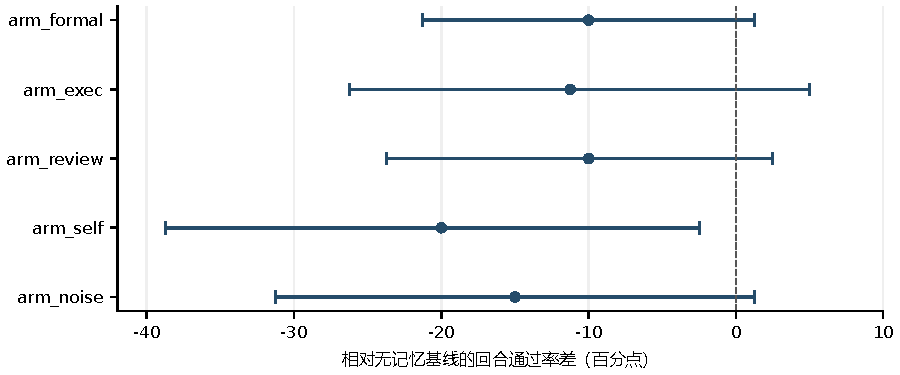
\includegraphics[width=\linewidth]{figures/generated/ch04-e02-effects.pdf}
\end{minipage}

\caption{验证层级与实际操作分开呈现。上方为综述的定性框架\cite{rsi-survey-2607}；
下方点与线段分别表示 E02 各记忆臂相对无记忆基线的通过率差和历史 95\% 题级自助区间。
数值来自表~\ref{tab:ch04-e02}，以百分点呈现；每臂 \measured{16} 题、每题 \measured{5} 个回合。
区间含零不表示等价，臂间差异应直接比较。此图保留旧估计，不替代完整验证层级的检验。}
\label{fig:ch04-ladder}
\end{figure}


\subsection{本轮的边界}
\label{sec:ch04-limits}

当前记录支持对六种已实现方案作描述，并提供反馈管道的故障案例。
它不支持“形式验证一定优于自评”，也不支持反方向的普遍断言。
新实验应重新冻结信息可见范围、反馈原文归档、任务内工具许可和成本口径，使用新运行标识。
旧轨迹不能因代码修复而被重新命名为新设计的观测。
E02b 与候选 P8 尚未执行，作为十个研究问题之外的扩展方向保留。

\section{反馈通道的相关错误：多看一眼为什么未必多一份证据}
\label{sec:ch04-correlated}

把作答者与评审者分成两个组件，是一种有用的结构安排，但组件数量不等于证据来源数量。两个请求若使用相同模型、相同材料、相近的提示，可能共同忽略同一处契约，也可能因为重新组织任务而发现不同问题。哪种情况占主导需要检查，不能由“独立评审”这个名字决定。

Reflexion 将行动、评估和语言反思分成不同角色，再把反思用于后续尝试；Self-Refine 则明确使用同一模型生成、反馈与修订\cite{reflexion-2303,self-refine-2303}。这些工作提供了不同的流程组织方式，不能仅凭角色图推断错误统计上独立，更不能把某项任务上的收益保证移植到任意模型与环境。

\subsection{相同模型、不同提示与独立证据是三个概念}

在 E02 中，评审提示把输入称作提交者的代码，自评提示把输入称作刚完成的代码。两者都通过同一个后端发起一个新请求；按保留实现，传入题目及含测试源码的文件渲染文本。自评请求没有继续原来的对话，也没有读取生成者的隐含状态。因而本次比较最多涉及这两类提示及其完整下游流程，不能声称隔离出了“他人判断”和“亲历者反思”的差异。

若要研究上下文影响，可以固定同一提交，比较只给代码、给完整执行轨迹、给截取的关键观察三种输入。若要研究评审模型差异，则应保持输入构造一致，再改变评审者。两项因素同时改变时，得到的是完整配置差异，仍有工程价值，但归因范围必须随之收窄。

更换模型也不自动消除相关错误。不同模型可能共享训练材料，面对同一缺失规格也都无法判断；同一模型在看到真正新增的测试反例后，反而可能修正先前错误。因此，应追踪新增了什么证据，而不只记录换了哪个名称。对栈案例而言，增加一个同样声称“逻辑正确”的评审不如实际检查一次状态变化；这是一种针对本例的诊断选择，不是所有任务都优先运行测试的定律。

\subsection{多数票需要先查共同盲点}

如果若干评审都读到同一份不完整材料，多数票可能只是在重复材料的偏差。例如题目要求“不修改调用者传入的列表”，评审输入却只保留返回值说明。多数评审都赞成原地修改，不能补回被删除的要求。这里应修复输入，而不是增加投票次数。

检查共同盲点可以从错误集合开始。对同一批候选分别保存各评审的判断，看看它们在哪些样本上同时失误、在哪些样本上互补。总准确率相近的评审，错误重叠可能很不同；总准确率较低的评审，也可能对某个关键风险提供独有证据。但选择评审组合的过程本身会使用数据，最终效果应留给未参与选择的材料检验。

如果只保存合并后的多数标签，后续就无法区分多数一致与少数异议，也不能检查仲裁是否压掉了有效反例。实际归档可保留每份意见、输入版本及合并规则，把合并结论作为派生结果。这样发生争议时，可以回到具体哪项证据被忽略，而不是重新让模型表决一次。

\subsection{理由相同不等于证据充分，理由不同也不等于相互独立}

语言表面上的多样性很容易误导。几位评审分别说“需要处理边界”“容器状态不正确”“可能有副作用”，可能都只是泛泛重述题目；一位评审说“长度没有减少”，另一位说“旧末项仍能再次读到”，却可能是在描述同一个可执行事实。评价互补性应落到观测与覆盖条件，而不是统计用了多少不同词语。

生成反馈时要求给理由，有助于让判断可审查，却不保证理由真实反映判断过程。因此，本书把理由视为一个待检验的文本产物。能核对它是否与代码和观察相容，能检查按它行动的效果；不能因为理由写得详细，就宣称已经测量了模型的真实因果机制。

这也解释了为什么“让模型更认真地反思”通常不是完整的实验操作。认真是一种提示措辞，可能改变长度、生成成本、关注点和回答风格。若预期收益来自更好的错误定位，就应记录定位是否更具体、更准确以及是否改善修复，而不只检查输出是否更长。

\subsection{信息冲突比一个错误标签更复杂}

E02 噪声臂提供了具体例子。实现翻转开头的验收判定后，仍附未改变的测试输出。当标题说失败而输出显示通过时，模型面对的是两条互相冲突的线索；它可以信标题、信日志，也可以编出第三种解释来调和冲突。这三种反应不同于在只有一个标签时被错误告知结果。

归档经验中确实出现了“本地测试全绿仍可能验收失败”和“公开测试全过不代表验收通过”的解释。这些文字来自被翻转标签的记录，并非我们事后杜撰；但它们也没有证据证明另有一个更严格的验收器实际失败。对不一致输入作合理化解释，是本例可见的风险。至于这些解释是否造成后续失分，还需要看检索和实际修改，不能由一句话直接判定。

若下一轮研究纯标签噪声，就只提供预先定义的标签，避免同时泄露原标签；若研究矛盾信息下的处理，则应把标题与日志的冲突作为独立因素，记录系统如何仲裁。若研究日志隐藏，除了删除总结行，还要考虑断言回溯、错误标记、用例名称和期望值。不同目的需要不同的遮蔽规则，不能用同一个“无判定”名称混合。

\subsection{反馈源的可信度需要具体到命题}

编译器可以可靠地告诉我们某种语言规则是否被接受，却不能因此替代产品需求的判断。测试可以指出一个输入上的输出错误，却未必覆盖性能与隐私约束。用户的纠正可以澄清其意图，但若不同用户有不同目标，就需要保留身份与任务上下文，而不是合成一个全局偏好。

因此，更有用的问题是“这个来源支持哪个命题、在什么条件下支持”，而不是给来源贴一个永远有效的可信等级。形式检查同样需要规格与检查器的假设；若证明的是一个写错的规格，证明正确也不会使产品满足真实需求。验证层级提示我们关注信号与外部约束的联系，不能让我们跳过被检查对象本身。

\section{迟到反馈：结果到达时，系统已经换了版本}
\label{sec:ch04-delay}

编程小题通常很快返回测试结果，用户复核、异步任务和业务结果却可能晚得多。反馈到达时，候选代码、记忆或工具版本已经改变。第\ref{ch02}章给出的版本与事件关联，解决的是把结果接回实际执行对象；本节进一步处理时间顺序怎样改变反馈的可用信息与评价分母。以下是设计示例，不是新增实测。

\subsection{按可用时刻释放反馈}

动作发生、反馈生成、系统接收是三个时刻，分别确定谁执行了动作、检查何时完成，以及更新器从什么时候起可以利用结果。离线重放若按任务开始时间排序，并在每题结束后立即写入后来才取得的全部结果，就给系统增加了当时不知道的知识。评价真实延迟下的在线更新，应按反馈可用时刻释放信息；评价标签齐备后的批量学习，则另行定义离线流程。

时间记录还需注明时区与时钟来源。不同服务未必同步，毫秒级字符串不保证毫秒级可比性。若只能确认先后顺序，就保存事件序列与时间范围，不据此推断更精确的因果顺序。

\subsection{旧失败先关联，再检查当前版本}

设候选甲处理任务后，系统已经切换到乙，随后才收到甲的失败结果。先用运行、输入与反馈请求标识找到甲的实际提交，再检查同一条件是否仍存在于乙。甲乙共享故障组件，旧反馈仍可能是有效警报；乙已修复该路径，直接回退反而可能恢复缺陷。对不能及时重现的外部故障，可以增加观察或限制相关动作，同时保留原因未定的状态。

相同题目可能在不同版本与权限下执行多次，不能仅凭题目文本关联。回调重复投递时，去重键应指向检查事件；相同的“验收失败”文字也可能来自两个真实任务。找不到原运行的反馈进入待核对区。检查器后来修错时，旧判定、修正及原因均应保留，才能解释系统当时为何采取某项更新。

接收、关联、诊断与经验发布还需能跨进程重启恢复，避免重复消费或正文与索引只写入一半。具体状态转换沿用第\ref{ch02}章的候选与发布约束；检验它们可在离线副本中于写入前后中断，检查是否丢记录或重复计数。这类故障注入验证反馈管道，不测量Agent能力。

\subsection{等待窗口也是评价条件}

旧版本的迟到失败不应混入新版本通过率；只统计新版本已经返回的快速成功，又可能高估它。报告需固定等待窗口，分别列出已返回的成功、已返回的失败和尚未返回，并说明各项分母及截尾处理。短期检查较易发现格式和接口错误，长期反馈可能揭示状态泄漏、维护负担或用户是否采用结果；较晚的结果也更容易受其他改动影响，不能一律称为更真实。

可以把近端指标用于快速筛查，再用较晚结果检验其代理关系。例如，测试通过是发布门槛，后续错误报告补充覆盖，两者保持各自分母。若将延迟结果回分配为早先动作的奖励，还需说明对应假设。经验的证据状态也保留时间线：先记“暂时通过已知检查”，观察窗口结束后再更新，避免把后来的确认倒填为当时已经确证。

\section{把下一轮反馈实验设计成能够回答的问题}
\label{sec:ch04-design}

发现旧设计的限制以后，最容易做的事是扩大题数，再跑一遍同样的装置。这样可能缩小某些区间，却不会把单元测试变成形式证明，也不会让两种角色提示成为两种独立信息源。下一轮应先决定要回答哪一个问题，再选择保留哪些差异、固定哪些条件。

下面给出一个尚未运行的设计框架。它不修改历史 E02 的协议身份，也不预先宣告能够判决 P2b。目的在于把“反馈有没有帮助”拆成规模与成本都可以说明的具体比较，避免一次试验承载互相冲突的解释。

\subsection{先区分固定提交的修复与连续任务的学习}

固定提交设计以候选代码为实验输入。每份代码在分配反馈之前已经确定，错误类型与初始质量不随反馈臂改变。不同修复者接收同一任务、同一提交、同一资源上限，只在指定反馈部分有差别。主要结果可以是修复后的独立检查通过率，辅助结果包括新增故障、调用量与修改范围。

这种设计的优点是容易追踪反馈作用于哪份代码；限制是它不研究系统怎样形成自己的错误分布。若实际部署中某种反馈会改变后续作答策略，固定提交比较就没有覆盖这种连锁影响。因此，固定提交适合诊断反馈组件，连续任务适合评估完整更新流程，二者可以前后衔接，不能互相替代。

连续任务设计让经验按时间进入记忆，测的是整个任务流中的表现。它需要冻结任务顺序或随机化规则、反馈到达规则、写入器、检索器、预算与起始状态。若某臂提前成功从而少写经验，这也是流程的一部分，不能事后强行补足相同条数而不计成本。分析单位还应覆盖经验共享造成的依赖：同一条任务流内的回合不能轻率地当作完全独立样本。

两种设计可以共享任务来源，但用于选择方案的数据和最终确认数据应保持用途边界。先用小规模固定提交诊断格式、输入与修订分支，再冻结连续任务方案，能够减少把工程故障误当理论负结果的风险。诊断阶段得到的分数仍应完整保存，不能挑出最好看的配置后把它称作未经选择的结果。

\subsection{把反馈操作写成输入差异表}

每一臂至少说明：是否见到测试源码，是否见到执行结果，是否见到明确标签，是否见到模型解释，是否继承原轨迹，以及反馈何时交给执行者。这些字段共同决定实际信息边界。只填“外部反馈”或“内部反思”无法让另一个实现者复现比较。

如果比较标签与诊断文本，可以让两臂都看到相同标签，只增加诊断内容；如果比较执行输出与模型意见，则必须明确模型意见是否已经读过输出，否则“意见”可能只是对同一输出的压缩。若要研究没有外部检查的自评，应核查题目附件、测试源码、缓存记忆和提示模板是否已经传入检查结果。

信息量与成本有时无法同时完全匹配。完整日志比一行标签长，模型读它需要更多输入；压缩日志又引入压缩器的选择。可以明确比较等调用上限、等总成本或实际配置三种不同问题，选择其中一种作为主要口径，再报告其他资源。不能把同样的回合预算说成所有环节资源相等。

\subsection{反馈档案应支持回放，也应支持否认过强结论}

每份反馈保存原始输入与原始输出，并保留经过截断、脱敏或格式修复后的实际展示版本。模型看到的是展示版本，审计需要知道它与原文差在哪。若只保存原文，无法确认被截掉的部分是否正好包含关键断言；若只保存摘要，无法核对摘要是否歪曲了原意。

不同权限下可以保存不同级别的材料，但缺失必须显式记录。敏感内容不宜为复现而无限复制；可在受控位置保留原文，在分析中使用引用与必要摘要。无论选择哪种方案，都不能在报告中声称记录了实际上没有保存的字段。E02 的中间模型评审原文缺失，就使逐字诊断审计受到限制；保留这个限制比事后重跑生成一段相似文字更诚实。

运行标识还需要绑定实际代码，而不仅是仓库当前提交号。E02 配置中的提交号早于其运行器进入版本库，现存代码与稍后首次提交一致，但缺少运行时的未提交差异与完整源码指纹。这不使所有轨迹失效，却限制了“逐字复现原运行实现”的承诺。新设计可以保存必要代码快照与配置散列，使之后的修复不会模糊旧实验身份。

\subsection{门槛、缺失与比较数量要在结果出现前说明}

诊断比较应预先定义主要结果和最小有用变化，并说明失败、超时、格式错误如何入账。格式错误既可能是接口不适配，也可能影响实际部署效用；若工程问题修复后重跑，应使用新版本和新记录，不能只替换旧数据中的失败行。报告可以同时给出完整方案表现与预定条件下的内容分析，前提是分母与选择规则清楚。

多个反馈臂之间可以产生许多两两比较。若看到结果后只挑一个有利差值，单个区间就不再代表整个选择流程的不确定性。主要比较应提前指定，探索性比较另列；需要联合判断完整排序时，还应考虑比较数量和方向约束。相邻两个点估计反序仅是描述，不能单独作为整条层级被推翻的判据。

样本规划还要考虑错误提交的构成。如果样本大多是已经正确的代码，评审者总说通过也可能获得高标签准确率，却没有展示定位失败的能力。可以报告成功与失败候选各自的判定表现，并按预定目标分布汇总。人为平衡样本便于机制检查，但总体指标应注明这种抽样，不能直接当成部署环境中的错误率。

\subsection{用停止规则保护问题本身}

工程试跑可以设置明确的停止条件：归档字段缺失、工具许可与声明不一致、任务材料越过信息边界，或账本不能闭合时，先停止扩大规模并修复。停止是为了保持实验身份，不能只在结果不好时启用。正式试验中的统计停止规则则另行规定，避免反复查看区间后在恰好有利的时刻收工。

最终报告应回答三个层次的问题：实际执行了什么配置，这批数据呈现了什么差异，这个差异支持原问题到哪一步。若第三层仍不能回答，可以保留有效的工程与机制发现，并明确待补设计。第16章的研究问题表将已有观察连到后续对照，每项试验按自己能够回答的问题报告。


\section{条件变化：先定位断点，再选择改动}
\label{sec:ch04-conditions}

如果结果标签本身与独立检查频繁冲突，先检查规格、环境和判定来源。
如果标签一致而诊断偏离证据，改进诊断输入或约束；如果诊断正确但未触发行动，检查执行与预算。
如果当前题修好而后续题受损，则查适用条件、检索和发布门槛。
这些分支可以并存，不能用一个低标签不一致率排除全部上游问题。

族间方向不同，提示应补充按族报告和任务分布分析；总体平均值仍可回答既定目标分布下的平均表现。
测试反复进入更新环节时，应保留独立检查，必要时按冻结方案扩展覆盖；轮换也会改变难度，不能把分数变化直接当进步。
在没有执行反馈的领域，仍可寻求可核对的原文、外部记录或人工纠正，并说明其滞后、主观性与覆盖范围。

\begin{principlebox}
先建立观察与候选版本的对应关系，再判断反馈值不值得写入。
标签一致性、诊断有效性、行动执行和迁移收益各自需要证据。
定性层级帮助提出比较，实际输入与实现决定比较究竟测到了什么。
样本规划不替代操作有效性；一次负结果也不自动提供负结果的原因。
\end{principlebox}

\section{非可验证前沿：方向生成在层级之前}
\label{sec:ch04-framing}

层级索引的是\textbf{方向评估}：给定一个候选方向，判断它是否成立、是否值得投入。
它不索引\textbf{方向生成}：哪些问题值得被评估，
以及何时一个仍被高分评价的问题已经不值得回答\cite{rsi-survey-2607}。
方向生成在逻辑上\textbf{先于}层级，不是层级的一级。

一个闭环可以爬到层级顶端、保持一个诚实的评估器、
检测到自己的代理指标被腐蚀，却仍然在一个早该放弃的问题上做得很好——
\textbf{因为层级把“问题”当作给定的}。
这类失效（原文称为 frame lock-in）的诊断难点在于观察边界：
前三类失效（自证循环、塌缩、多样性塌缩）
可能在内部指标上留下线索，而目标是否值得优化往往还需外部需求来判断\cite{rsi-survey-2607}。

把这条放回本章的实验：
E02 的六个臂都在回答同一批给定的 \measured{16} 道题，
这些比较也答不了“这 \measured{16} 道题值不值得被回答”。
这是第 16 章要处理的问题，本章只把边界划出来。

% ---------- 6. 反例 ----------
\begin{pitfallbox}
\textbf{把后来正确的解释，倒填成当时正确的行动。}
栈案例中的经验正确指出删除操作缺失，但原回合已经结束。复述经验不能改变提交记录。

\textbf{把相同臂名，当作相同信息边界。}
自评提示声称没有测试结果，并不意味着它没有测试源文件；新建上下文也不等于拥有独立判断来源。

\textbf{把接近的调用数，当作完整成本相同。}
六臂调用数依次为 \measured{431}、\measured{403}、\measured{406}、\measured{408}、\measured{409}、\measured{407}。
这些总数已含记忆生成和模型评审的旁路调用，不应再把 \texttt{side\_calls} 加一遍。
账本中每臂约 \measured{332}--\measured{385} 秒是回合计时之和，未完整包含旁路调用等耗时，不能称为各臂端到端墙钟。
\end{pitfallbox}

\section*{习题}
\begin{enumerate}[label=4-\arabic*.,ref=4-\arabic*]
  \item\label{ex:ch04-1} 表~\ref{tab:ch04-six} 的六类信号是代码特有的。
        为你熟悉的一个非编程 Agent 场景（检索问答、数据分析、流程自动化）
        补出对应的六类信号，并标出其中哪几类可重放。
  \item\label{ex:ch04-2} 本章区分“反馈标签一致性”和“迁移收益”。
        请构造一个例子，使得标签不一致率为 0 而收益为负（提示：想检索环节），
        再构造一个使标签不一致率高而收益为正的例子。
  \item\label{ex:ch04-3} 表~\ref{tab:ch04-adj} 按旧臂顺序出现一次点估计反序（执行输出 vs 评审提示，
        点估计 \measured{$-0.0125$}）。
        请列出三种能产生这种反转的\emph{设计}原因（不是“真实就是这样”），
        并说明各自应当如何被排除。
  \item\leavevmode\label{ex:ch04-4}E02 已有 \measured{16} 道配对题，区间精度公式给出约 \calcnum{592} 道独立题的规划示例。
        扩题、增加每题重复次数、改用分层估计，分别处理哪种不确定性？
        为什么后两项不能直接算作增加了独立题数，这个规划数又为什么不是功效保证？
  \item\label{ex:ch04-5} 第 \ref{sec:ch04-framing} 节说方向生成先于层级。
        设计一个可观测量，使得“一个闭环正在优化一个不值得优化的目标”这件事变得可检测。
\end{enumerate}

\section*{常见误解}
\begin{itemize}
\sloppy
  \item \textbf{“反馈越可靠，收益越高”。}
        E02 中有四臂各自的 \measured{8} 条训练标签都与验收一致。其中两臂的标签直接取自验收结果或退出码，另两臂来自模型评审或自评。到了封存题，四臂的通过率点估计均低于无记忆基线，只有自评臂的差值区间完全低于零（表~\ref{tab:ch04-e02}）。
  \item \textbf{“E02 说明验证层级是错的”。}
        本轮的反馈操作并未覆盖完整概念层级，且样本与确认性设计仍有缺口，本轮不能由该排序推出完整反馈层级的规律。
        区间包含 0 与一次反转都只作为读数，不构成判决。
  \item \textbf{“有了测试就有接地，自进化就能跑起来”。}
        固定基准存在过拟合与投机风险\cite{rsi-survey-2607}；
        接地需要维持独立检查及适当覆盖；轮换与留出检验须按协议进行，也不能代替对规格的核对。
  \item \textbf{“第 4 层最便宜，所以从它开始最划算”。}
        原综述将其概括为低成本、易投机的信号\cite{rsi-survey-2607}，并未给出适用于所有任务的费用排序。
        自一致性可能需要多次采样，执行一个简单断言也可能很便宜；成本与失效风险均须按具体流程测量，不能从定性层级直接推出部署策略。
\end{itemize}

\section*{进一步阅读}
\begin{itemize}
\sloppy
  \item \cite{rsi-survey-2607}：验证层级四层（\S 5.2）、包含frame lock-in在内的四类失效模式（\S 5.3）、
        方向生成与方向评估之分（\S 5.4）的出处；
        本章表~\ref{tab:ch04-hier} 与 \S\ref{sec:ch04-framing} 采用其概念讨论。
        读它时务必保留原文那句"not a measured law"。
  \item \cite{coding-survey-2608}：六类代码特有信号 E/D/T/R/Q/H 与 Figure 7 的占比统计，
        本章表~\ref{tab:ch04-six} 的数字来源；\S 4.1 的边界判据（学习信号必须来自自身尝试）
        是第 1 章 1.1 的另一处依据。
  \item \cite{ksi-2607}：带适用条件的知识条目（\texttt{applies\_when} /
        \texttt{does\_not\_apply\_when}），本章 \S\ref{sec:ch04-hypothesis} 的设计规则来源。
  \item 本书第 3 章：配对差、重采样单位与 MDE 的口径；
        第 14 章：评审者本身成为优化目标时（自证循环）会发生什么；
        第 16 章：方向生成与 frame lock-in 的最终处理。
\end{itemize}

% chapters/ch05.tex —— 第 5 章
% 体例：具体失败 → 设计问题 → 机制解释 → 对照实验 → 条件变化 → 选择原则
% 数字身份纪律：A-Mem / Trap of Trajectory / KSI 的数字一律 \cited{}（出处见 source-map 第 5 章各条）；
% E03 / E03c 的本书实测一律 \measured{}；由实测算出的量用 \calcnum{}。
\chapter{记忆如何转化为可复用的经验}
\label{ch05}

\chaptergoal{保存更多历史，为什么不一定更会做事？}
\chapterprops{P3（形式与容量如何共同影响迁移）与
P3b（拟合目标怎样影响迁移）。本章用E03与E03c的观察解释表示、读取者与比较范围之间的关系。}
\chapterfig{图~\ref{fig:ch05-fit}：一条经验可以拟合到求解器，也可以拟合到问题域}
\chapterpitfall{把``存下来了''当成``学会了''；把检索到的相关性当成因果；
把同族新题上的提升当成跨族迁移}

% ---------- 1. 具体失败 ----------
\begin{failurebox}
第 4 章的栈错误，在另一项实验中又成为一条经验来源。
E03 拆分 A 的同一份失败记录，被渲染成三种形式：截取记录、短摘要、结构化经验。
短摘要明确指出需要删除并返回栈顶；结构化条目进一步说明，查看栈顶的场景不应照搬这个操作。
名为 \texttt{form\_raw} 的条目却在 \measured{600} 个字符处硬截断，
代码停在 \texttt{push} 方法的一部分，还没有出现出错的 \texttt{pop} 方法。

“保留原始记录”这个名字，并不表示关键信息完整保留下来。
与此同时，不同渲染改变了检索排名：拆分 A 的 \measured{16} 道留出题中，
结构化与摘要选择的来源条目集合有 \calcnum{12} 道不同；截取记录与摘要有 \calcnum{14} 道不同。
这些差异已与实际系统提示逐项核对。

所以本章不能只问哪一种记忆文字更好。还要问：
什么被写下、什么被截掉、什么被取出，以及读到它的系统最终做了什么。
\end{failurebox}

\designquestion{判据不是``记住了多少''，而是：
\textbf{这条经验在换了一件事之后还成不成立}。
换一道题、换一个族、换一个读到它的模型——
每一种变化都可能改变经验的适用性，这一步必须可检查。}

\section{同一段经历，为什么会写成三种不同的经验}
\label{sec:ch05-same-source}

同源材料是一个重要控制，却只是控制的起点。E03 先让无记忆 Agent 产生来源记录，再从同一条记录渲染不同形式。这样避免了为摘要选一批容易题、为结构化经验另选一批难题。渲染完成以后，内容覆盖、长度、措辞和检索排名仍可能分化。若把“同源”直接解释成“其他都相同”，后面的归因就会跳过这些实际变化。

\subsection{栈记录中保留与丢失的内容}

拆分 A 的栈来源记录包含失败验收和最后代码。归档的短摘要说，应同时返回并移除栈顶，可以使用容器的弹出方法，不能只读末元素。结构化版本则分成事实、适用、不适用三行：事实指出只返回未删除；适用范围是实现需要改变内容的弹出操作；不适用范围是只查看栈顶而不能修改内容的操作。

这两份文本都比原始记录短，却保留了诊断的关键。它们之间的区别也不只是字段名：结构化版本明确写了相反需求，短摘要更直接给出代码操作建议。若后续行为不同，可能来自条件边界，也可能来自具体操作提示、措辞长度或读取者对格式的反应。要分离这些因素，需要设计新的受控版本，旧运行没有同时完成所有消融。

截取记录臂提供了另一种取舍。它按固定顺序拼接源题、工具名称、验收状态、部分验收输出与代码，然后取前 \measured{600} 个字符。在这条失败记录里，错误回溯和临时文件路径占据了前部空间，末尾代码被截到 \texttt{push} 的一部分。恰恰需要检查的 \texttt{pop} 函数没有进入条目。

因此，“原始轨迹”在这里是历史臂名，不是逐步完整档案。条目中没有完整保留每次工具参数、每段模型回答或全部观察，连拼接后的记录也会截断。完整任务轨迹仍可用于审计，但被注入下游上下文的是这个短片段。评价经验形式时，应描述实际展示给读取者的材料，不能用归档材料的完整性替代提示内容的完整性。

这个例子也说明，固定字符上限并不保证各条经验受到相同程度的压缩。成功输出通常短，失败回溯可能长；同样的拼接顺序会使失败记录留下更少代码。如果长期按此规则处理，保留内容可能系统性地随结果类别变化。这里提出的是可检查的设计风险，不是未经统计就断言所有失败记录都会丢失关键内容。

\subsection{长度口径决定了“同容量”究竟是什么意思}

拆分 A 每种形式各有 \measured{8} 条条目，平均长度分别为截取记录 \measured{600}、摘要 \measured{44}、结构化 \measured{102.75} 个字符。这里的字符按 Python 字符串长度计数，包含中文、英文、数字、空白与标点，不是汉字数，也不是计费 token 数。拆分 B 的求解器文本与问题域文本平均长度分别为 \measured{60.75} 和 \measured{104.375} 个字符。

相同条目数控制了存储单元数量，没有控制上下文长度。即使每次都取两条，注入的字数和 token 数仍不同；即使把字符数截成相同，模型分词后的 token 数也可能不同。容量可以指条目数、磁盘字节、索引大小、检索条数或提示预算，必须选定所研究的那一种。

长度还不是内容量的充分代理。重复模板、路径和测试框架文字占字符，却未必提供当前任务需要的信息；一个短条件可能排除大量错误操作。反过来，删掉具体输入只留下抽象口号，也可能使诊断失去依据。因此，应把长度当作资源约束，把信息覆盖作为另一个需要检查的对象，而不是认为压得更短就必然更好。

原提示要求摘要不超过一段较短文字，但实现还有自己的字符截断。提示中的限长是一项请求，实际输出长度才是观测。归档中确有摘要条目超过提示宣称的字符数量，不能把提示目标直接写成严格执行的上限。对可复现实验，存储前后的长度与最终展示长度应分别可查。

\subsection{改写经验也改变了哪些经验被看到}

E03 沿用字符二元组检索。去掉空白后，将查询和条目分别变成相邻字符对的集合，按查询与条目共同字符对的数量除以条目字符对数量排序。这个分母来自候选条目，不是两个集合的并集，所以它不是常见的 Jaccard 系数。长文本若增加了许多不与题目重合的字符对，分数可能下降；较短文本若保留了几个匹配词，分数可能上升。同分时，保存列表中位置较后的条目优先。因此，复算检索结果还需要保留条目顺序。

这不是说长文本总被惩罚，或者短文本总被优待。新增词语也可能提高交集，具体排序由两部分共同决定。但格式字段、代码标识、自然语言同义表达都会改变集合，故“只改存储形式、检索器没改”仍不等于检索结果相同。检索器的函数固定，输入表示变化也会改变输出。

离线复核使用归档经验与实际任务陈述重建排名，并将选中文字与原始系统提示逐项比对。拆分 A 的三种记忆臂共核对 \calcnum{240} 个提示，拆分 B 的两种同模型记忆臂共核对 \calcnum{160} 个提示，选中文字均出现于对应提示。拆分 A 中，结构化与摘要的源条目集合在 \calcnum{12/16} 道题上不同，截取记录与摘要在 \calcnum{14/16} 道题上不同；拆分 B 的两种拟合目标也有 \calcnum{12/16} 道题不同。

例如标准拆分中的 \texttt{classstate-07}，求解器文本选中了异常契约题与栈题的经验，问题域文本选中了计数器题与可变默认参数题的经验。仅这一处就足以说明，读取者看到的不是相同两条事实的不同排版。它还不能证明哪一组更适用，更不能证明哪条经验导致成败；那需要继续看任务契约、实际行动和反事实对照。

\subsection{把检索变化视为机制，还是视为混淆}

答案取决于问题。如果研究的是“把整个经验系统从摘要切换到结构化格式会怎样”，检索变化就是完整方案效果的一部分，应保留并报告。如果研究的是“在相同经验内容已经被选中时，加上条件字段是否改善执行”，那么检索变化就是需要控制的中间路径。

后一种设计可以先固定来源条目标识，再渲染各版本给读取者。这样切断了形式经由检索排名影响成绩的路径，却也偏离了实际自动检索流程。前一种设计更接近部署，后一种更适合拆解机制。两种结果可以并列，但不能用一种设计的区间回答另一种设计的问题。

还可以增加一个中间检查：固定检索器与经验来源，记录每道题选中的来源集合、顺序和展示长度。若整体成绩变化，这些记录有助于定位下一步该做哪项干预。它们仍属于机制观察，不能仅凭“更相关的经验出现得更多”就宣称中介效应已经被识别。

\subsection{先确认信息还在，再检查能否取出}
\label{sec:ch05-construction-retrieval}

同一个错误答案可以来自不同环节。以章首栈记录为例：若条目已丢掉“移除栈顶”的要求，单换检索器不能恢复这个条件；若条件仍在库里，却没有进入提示，应先查候选选择；若正确条件已经展示，执行者仍只读取末元素，就要查它怎样理解并使用经验。这些路径可以并存，需要逐题沿保存内容、检索结果和实际动作核对。

Zhou 等在 LongMemEval-S 与 BEAM-100K 上比较六种显式记忆和原始历史 RAG，固定已构建的记忆，再改变检索器与上下文预算。显式构建没有取得稳定的总体优势，收益集中于部分题型和受限条件\cite{raw-history-memory-2610}。其控制保留了各系统周边的查询规划、链接扩展等流程，不能当作只改变文本表示的纯形式实验。

该研究还按标注的支持语句追溯来源，构造不受实际检索排名约束的参照\cite{raw-history-memory-2610}。这有助于定位检索瓶颈，却不是可部署的读取策略；来源范围重合，也不保证改写后的条目完整保留答案。若直接提供候选支持材料后仍答错，还应检查表达与读取能力，不能仅凭答案错误就断言信息已经被删除。

\section{从一次经历抽象出规则，哪些细节可以删除}
\label{sec:ch05-abstraction}

抽象的目标不是让经验听起来更普遍，而是在保留必要条件的前提下去掉偶然细节。需要删除的可能是临时路径、无关对象名与重复日志；需要保留的可能是异常契约、状态是否共享、输入能否修改，以及失败出现的具体边界。对每项细节都可以问：如果它改变，建议是否还成立？

\subsection{按变量作用区分必要条件与背景}

以下是本书构造的教学例子。某次文件处理任务要求读入数据、按指定键排序并输出新文件，原文件必须保留。失败发生在输出覆盖原文件之后。路径里的日期、用户名和临时目录通常属于背景；“输出与输入不能是同一目标”则直接连接到失败条件。若把经验写成“不要用昨天的路径”，保存的是一次偶然关联；写成“写入前核对目标与受保护输入是否相同”，才指向可检验的机制。

抽象仍不能过宽。某些任务本来就要求原地转换，并有备份和恢复保证；一律禁止同路径写入会改变需求。更合适的条件是“在输入必须保持不变的任务中”，再给出检查动作。反例不是为了把经验写得冗长，而是防止一条正确的局部规则抢占所有场景的决策权。

判断某个细节是否必要，可以构造最小变化：只改目录名、只改输入内容、只改是否允许覆盖，再检查原建议是否仍然合理。这些变化可以先由规格分析完成；需要程序行为支持时，再做受控执行。若同时改变任务目标与运行环境，观察到不同结果也无法知道哪项条件真正重要。

\subsection{从成功中提炼经验，也要保留不确定性}

成功轨迹往往包含很多不必要动作。系统先读了一份无关文档，后来凭已有知识完成任务；若摘要把整个顺序都写成成功步骤，就会把无关读取固化为前置条件。下一题照做这些步骤，可能只是增加成本，也可能引入错误信息。

因此，成功经验可以分成已观察事实与候选策略。事实是这次使用某个版本、完成某个结果；策略是以后遇到某条件可以尝试某动作。后者需要更多证据，尤其要检查省掉这个动作是否仍然成功。没有反事实比较时，可以说“本次有效流程的一部分”，而不应说“成功所必需”。

失败经验同样有这个问题。一次失败后换了多个设置才成功，不能把最后一次改动自动认定为原因。把中间候选及检查结果保留下来，可以更准确地界定目前知道什么；无法分离的联合修改，就先作为联合策略记录。过早概括为单一规律，会让经验更容易检索，却更难正确使用。

\subsection{事实、解释与建议不要互相冒充}

一个条目可以写“该输入下返回空集合”，也可以写“因为默认值共享导致状态丢失”，还可以写“改用独立容器”。第一句是观察，第二句是解释，第三句是干预建议。它们需要不同的支持材料。观察可以由日志核对，解释需要与其他可能原因竞争，建议需要检查修改后的后果。

若把三句压缩成“默认容器错误”，下游既不知道出错的是共享还是清空，也不知道返回空集合究竟违反了什么要求。简短到无法恢复推理对象的经验，可能只剩一个关键词。结构化并非必须使用固定字段名，但应让这些逻辑角色可区分，否则一句推测很容易在反复转述中变成“已证事实”。

KSI 的条目模式把适用条件、不适用条件与证据并列\cite{ksi-2607}，提供了一种实现方式。本书借用的是可检查边界与来源这一思想，不把特定字段名当通用正确性保证。若字段里只是“适用于类似情况”“不适用于不同情况”，形式合格，信息仍然不足。

\subsection{保留一个能推翻规则的测试}

经验条目不必随身携带庞大测试集，但最好指出什么观测会使它失效。例如“输入必须不变”可以由调用前后比较检查；“这个接口返回新对象”可以由对象身份与内容分别检查；“该操作能安全重试”则需要检验重复调用是否产生额外副作用。

这种反驳条件能把经验从口号变成可维护的资产。新版本出现反例时，系统可以判断是条件范围过宽、环境假设过期，还是原规则本来就不成立。若只保存“通常这样更好”，几乎任何失败都能被解释成例外，经验便很难真正被修订。

并非所有知识都能立即形式化。对于写作风格或复杂业务判断，可以保留任务样例、用户选择和争议说明。关键是不要伪装成更强的证据：偏好例子支持特定情境下的选择，不自动成为跨用户的质量定律。抽象要提高可复用性，也要保留我们尚不知道的边界。


\section{四种形态：轨迹、事实、策略与程序}
\label{sec:ch05-forms}

\begin{table}[htbp]
\centering
\caption{经验的四种形态：常见检索线索与典型失效方式}
\label{tab:ch05-forms}
\begin{tabular}{>{\raggedright\arraybackslash}p{2.2cm}>{\raggedright\arraybackslash}p{4.0cm}>{\raggedright\arraybackslash}p{3.6cm}>{\raggedright\arraybackslash}p{3.3cm}}
\toprule
形态 & 一条是什么 & 常见检索线索 & 典型失效 \\
\midrule
轨迹 & 一次完整尝试的原始记录 & 与当前任务的表面相似 & 长、噪声多、含大量与成败无关的步骤 \\
事实 & 关于世界或任务域的一条陈述 & 实体与条件 & 过期；被更晚的事实覆盖 \\
策略 & ``遇到 X 就做 Y''的 conditional & 条件匹配 & 条件写得太宽，于是被套到不该套的地方 \\
程序 & 可执行的一段代码 & 签名与前置条件 & 接口漂移；依赖消失 \\
\bottomrule
\end{tabular}
\end{table}

表~\ref{tab:ch05-forms} 的四行不是并列的优劣排序，而是四种不同的失效方式。
本书第 7 章处理的是``事实与策略''被写进上下文的形态，第 8 章处理``程序''；
本章关心的是它们共同的前置问题：\emph{一条经验凭什么被留下}。

\section{筛选、抽象、合并与冲突处理}
\label{sec:ch05-curate}

A-Mem 把一条记忆写成一个带七个字段的笔记
$m_i=\{c_i,t_i,K_i,G_i,X_i,e_i,L_i\}$：内容、时间戳、关键词、标签、上下文描述、
embedding 与链接集合\cite{amem-2502}。
新笔记写入时按余弦相似度
（假定两个嵌入向量均非零）

\begin{equation}
s_{n,j}=\frac{e_n\cdot e_j}{\lvert e_n\rvert\,\lvert e_j\rvert}
\label{eq:ch05-link}
\end{equation}

取 top-$k$ 近邻，再由模型决定是否建立链接，并对近邻做一次演化\cite{amem-2502}。

\begin{sloppypar}
成本需要连同计量对象一起读。A-Mem 的成本段报告每次记忆操作约 \cited{1{,}200} 个 token，
并汇总相对于约 \cited{16{,}900} token 基线的 \cited{85--93\%} 降幅；
单次低于 \cited{0.0003} 美元是该论文当时的接口成本报告，不是当前报价\cite{amem-2502}。
这两个近似 token 数直接计算只能得到约 \calcnum{92.9\%}，不能独自推出整个降幅区间。

原文表 1 另列回答一道问题的平均 token 长度：GPT-4o-mini 配置为 \cited{2{,}520}，
GPT-4o 配置为 \cited{1{,}216}。这些表格数与成本段的操作口径应分别保留，
不能把约一千二百写成所有模型、所有写入与读取流程的统一费用。
若要比较完整生命周期，还需列出初始化、链接生成、近邻改写、检索和回答各自发生多少次，
以及哪部分已经计入原报告。论文的局部成本优势值得研究，但不自动证明完整方案更省或经验更正确。
\end{sloppypar}

\begin{principlebox}
\textbf{按实际消融读模块贡献。}
A-Mem 的表 3 比较同时去掉链接生成与记忆演化、仅去掉记忆演化、以及完整方案\cite{amem-2502}。
这支持所测试配置下的模块比较，不能说原文完全没有“有内容、无链接”的参照。
但它也不是在其他输入与读取过程逐字不变时，仅开关图边的纯拓扑实验。
若要把收益进一步归因于某种链接结构，需要针对这个问题另设控制。
\end{principlebox}

删除、改写与降权解决不同问题。A-Mem 的方法描述重点是笔记、链接与演化，
不能仅凭没有独立删除模块就推断所有矛盾必然保留。
其他方法即使没有单独的“删错惩罚”，删除也可能通过下游成绩受到间接反馈。
真正需要审查的是：错误条目怎样停止影响行为，误删以后怎样恢复，以及这些结果有没有被测量。

\section{合并经验时，怎样保留证据而不制造共识}
\label{sec:ch05-merge}

同一个问题被多次遇到以后，经验库里会出现许多相似条目。简单追加会增加检索负担，直接合成一句“共同规律”又可能抹掉差异。合并应先辨认重复的是文字、事件还是主张：三条文字相近的经验可能来自三次独立观察，也可能都转述同一次失败；三条措辞不同的经验也可能指向同一个条件。

\subsection{先去重事件，再合并主张}

如果一份失败报告被摘要器、审校器和汇总器分别改写，最后得到三个条目，这仍只有一个来源事件。把条目数当证据数，会使多次转述获得不应有的权重。每条派生经验应指向最初的运行或外部来源，合并时沿来源关系去重，而不只比较最终文本。

反过来，两个独立任务都出现同一种错误，即使最终经验句完全一样，也不应丢掉第二次观察。可以保留一份规范表述，并把不同证据挂在其后，分别记录各自条件。这样减少提示中的重复，又不牺牲证据的覆盖。若两次任务共享同一测试模板或同一环境缺陷，它们的独立性还要进一步限定。

一个实用的记录方式是分开“条目标识”和“主张标识”。条目标识对应某次具体写入，主张标识对应被维护的命题。若某条写入后来被发现是误转述，可以撤销这份支持而不必抹掉其他来源；若主张本身错误，则应沿主张关系检查全部派生建议。这个结构是本书的工程建议，不是现有 E03 归档已经具备的能力。

\subsection{条件不相同，先分支，不急着选边}

考虑两条教学示例：“转换失败时返回默认值”和“转换失败时应抛出错误”。它们看起来冲突，实际上可能来自不同接口契约。一个交互式表单希望继续处理其他字段，另一个底层校验库要求调用方明确处理错误。先补齐调用场景与接口要求，矛盾可能变成两个条件分支。

合并后可以保存共同部分：转换存在失败分支，失败行为必须符合调用契约；两个具体分支分别保留。若直接多数投票，常见场景可能淹没较少见但同样正确的契约。经验数量多，不代表它有权覆盖当前任务的明确要求。

也有真正冲突：两个条目针对同一版本、同一输入范围、同一目标，却分别声称某操作会与不会修改输入。此时需要回到来源或实际检查，而不是加一句“视情况而定”。条件已经相同，继续模糊条件只会回避问题。若证据暂时不足，保留争议状态并限制自动使用，比任意择一更可追溯。

\subsection{合并不能把窄证据扩成宽命题}

两条经验分别说某函数在空列表和单元素列表上正确，合并以后不能写成“适用于任意长度列表”。被观察条件的并集只有这两个范围，不是所有可能输入。类似地，两个模型都能读取某条经验，不代表它对任何模型可移植；两个时间点都有效，也不证明期间每个版本都有效。

经验摘要常会为了简洁删掉限定词，合并比单次摘要更容易发生这种扩大。可以在合并前后比较主张范围：新版允许哪些原来未允许的输入、动作或环境？如果出现新增范围，必须把它标成待验证扩展，而不是默认为已有证据的一部分。

合并也可以缩小范围。若旧条目声称所有可变对象都应该复制，后续发现某个接口明确要求原地修改，就应收窄到需要保持调用方对象不变的情况。这不是“记忆退化”，而是知识边界变得更准确。效果评估仍需检查收窄以后是否影响目标任务，但不能只按条目变短或变长判断好坏。

\subsection{版本关系比覆盖写入更适合解释变化}

用新文字覆盖旧文字很方便，却会使历史行动无法解释。某次任务遵循的是旧条件，审计时只看到已经修正的新条件，便可能误判执行者违背了当时规则。更好的做法是保留版本关系：新版取代哪一版，改变了哪些条件，依据哪份证据，何时对读取者生效。

读取时通常只展示当前有效版本，审计时仍能回到历史版本。这样不必把旧错误持续放进提示，也不必删除形成错误的过程。版本保留与提示可见性是两项不同决定，不能用“需要审计”作为永远启用旧经验的理由。

CALM 提供了一个将两项决定分开的实例。在其预定义的关系规则下，强冲突更新把新记录置为 \texttt{ACTIVE}、旧记录置为 \texttt{SUPERSEDED}，同时保留替换指针与有效时间边界\cite{calm-2610}。明确询问过去的查询，可让后端提供且满足内容、时间条件的查询局部副本进入本次使用筛选；旧记录的持久状态保持不变\cite{calm-2610}。这些规则规定记录何时可被采用；状态转移本身不能替代对争议事实的核查。

若条目被许多其他经验引用，合并还涉及依赖迁移。新主张是否保留了被引用的条件？原引用是支持例子、反例还是实现来源？统一重定向链接可能把反对意见变成支持意见。维护关系时应保留边的含义，而不只是让链接不报错。

\subsection{链接的价值在于可追踪关系，不是边越多越好}

A-Mem 通过近邻检索和模型分析建立关联，再更新相关笔记的描述\cite{amem-2502}。这使新经验能够改变旧经验的组织方式，但也把链接质量交给了具体表示与模型判断。语义接近的两条记录可能是支持、反例、同一来源的重复，或只共享任务名；把这些关系都视作相互强化，会丢失重要区别。

在工程实现里，可以为链接保留简单类型与来源。支持关系需要说明支持的是哪部分主张，冲突关系需要说明条件重合在哪里，派生关系需要说明转换步骤。若类型由模型生成，仍需接受检查和修订。类型越细，维护成本越高，不能把复杂图结构本身当作效果证据。

评价链接作用时，可比较相同内容下不同读取策略，也可比较完整链接维护方案与简单检索。前者帮助定位结构贡献，后者衡量实际系统价值。无论选择哪种，都应记录新增构建与维护成本。一个没有带来可测收益的复杂关系网，仍可能适合人工审计，但不应被直接称为更强的自主学习能力。

\section{经验生命周期：候选、启用、限制与撤销}
\label{sec:ch05-lifecycle}

经验保存以后，并不只有“存在”与“不存在”两种状态。刚从一次失败生成的建议，证据强度与经过多种任务检查的规则不同；某个版本失效的程序，也可能在旧环境里仍然有效。用生命周期状态表达这些差异，可以让读取者知道一条经验获得了多大的使用权限。

以下状态设计用于说明维护逻辑，不是要求所有系统照搬固定枚举。最小系统可以更简单，但要能区分尚待核查的候选、当前允许使用的条目、已知范围收窄的条目，以及不再进入自动检索的撤销条目。状态转移应由明确证据或管理决定触发，不能仅靠文字中的高置信语气。

\subsection{候选经验不应自动继承执行权限}

一次成功可能产生有价值的线索，也可能产生对无关步骤的赞美。候选区的作用是让线索可保存、可检查，同时限制它立即支配后续行动。对于低风险的检查提醒，可以允许以建议形式呈现；对于会执行写入、删除或网络动作的程序，准入需要覆盖前置条件、权限与回退。

把候选与启用分开，并不必然意味着每条经验都要人工审批。规则检查、离线回放、独立测试和预先授权的策略都可以承担不同环节。关键是门槛与后果相称，并且来源能够追溯。一个提醒“检查空输入”的条目，与一个自动修复所有空输入分支的脚本，不应因为共享同一句经验而获得相同权限。

准入失败也有保存价值。例如某条建议在本题修复成功，却损害另一项接口要求，可以作为反例保留。反例应进入合适的读取位置，避免被一般相似度检索误当正向规则。记录“尝试过且不成立”，有时比再生成一条近似建议更节省资源。

\subsection{启用状态应绑定环境与读取方式}

同一条自然语言经验，作为提示中的弱提醒与作为工具执行前的强制规则，作用不同。条目通过哪种读取方式的验证，就应限定在哪种方式下使用。把验证过的提醒直接升级成自动阻断条件，会改变系统行为，而不只是改变界面显示。

环境绑定也不能只写一个软件版本号。经验可能依赖返回格式、权限、数据类型或任务目标，其中一些变化不会触发版本号更新。记录可以优先保留与主张直接相关的条件：接口返回空值还是错误、容器是否可变、调用能否重试。只有需要时才扩展到完整环境快照，避免元数据越来越多却没有帮助判断。

读取者变化以后，启用状态需要重新检查。模型能解析三个字段，不代表它会遵守不适用条件；工具能加载一段程序，也不代表当前依赖满足。兼容性检查回答“能不能读”，行为检查回答“是否按预期用”，迁移评估回答“总体是否有益”，三者不应合并成一次加载成功。

\subsection{限制使用往往比立刻删除更准确}

新反例可能只影响一部分条件。例如经验要求在缺省参数下新建列表，但系统后来加入需要跨调用共享的缓存接口。此时可以排除缓存接口，而不是宣布经验全部错误。范围收窄有助于保留原先有效的部分，也能让后续读者知道为何存在例外。

若错误来自过期事实，则可以把旧条目限定到历史时间范围。例如某个接口曾经支持一项参数，后来移除；历史任务审计仍可能需要旧信息，当前调用则不应使用。时间适用范围与存储保留期不同，不能因为旧事实仍有历史价值就继续让它参与当前决策。

当无法可靠表达边界，或者误用代价太高时，可以先停止自动检索，将条目保留供检查。停止使用不表示我们已经找到全部原因；它是一项受证据不足约束的管理动作。应记录触发事件与恢复要求，避免条目在下一次重建索引时又无意恢复。

\subsection{撤销要覆盖派生物与缓存}

删掉经验正文，只能保证这个文件消失。它可能已经被写进提示模板、摘要、嵌入索引、技能说明或其他条目的合并版本。若这些派生物继续存在，系统仍可能使用同一错误建议。撤销需要沿来源关系定位影响范围，并检查哪些副本应删除、重建或标为失效。

并不是所有派生物都必须一起废弃。一个摘要可能同时引用多份独立证据，撤销其中一份后，其他证据仍然支持较窄主张。此时应重新评估支持关系，而不是机械级联删除。缺乏来源链时，这种精细处理很难完成，只能采用更保守的停用或重建策略。

缓存也需要版本意识。索引重建成功并不保证正在运行的执行上下文已经刷新；执行上下文可能继续携带旧提示。可以在任务边界核对经验版本，必要时中止会受影响的操作或重新构造上下文。处理方式取决于风险与系统能力，但不能把存储层的删除时间直接当作所有执行者停止使用的时间。

LEDGER v1 在其合成编码负载中，分别检查送给回答模型的证据和最终答案是否仍含被删除的值\cite{ledger-2611}。这两个检查回答不同问题：答案里没有出现该值，并不能证明它没有进入模型输入。论文列明，删除操作不覆盖旧快照、响应缓存和运行日志；这些副本需要另行规定保留与清理规则。

\subsection{遗忘策略需要看机会成本}

经验库容量有限时，维护者必须决定留下什么。按最近使用淘汰容易实现，却可能删除少见但关键的失败边界；按引用频率保留，又可能让经常出现的错误建议永久占据空间。使用频率反映流量，不直接等于因果价值或风险价值。

可以把评估问题写得更具体：删除某条经验后，哪些任务的行为可能改变？这种改变的收益、损失与维护成本如何比较？若没有足够数据估计单条贡献，可以按内容类别、风险和证据强度采用明确规则，并记录规则的适用范围。不要给每条经验编造一个看似精确、实际没有依据的价值分。

主动遗忘也有实验成本。为了判断一条经验是否有用而反复调用模型，可能比保留它更贵；为了降低提示长度做大量压缩，可能引入新的错误。维护策略本身需要计费与评估。第 13 章会把这些成本放进完整生命周期，本章先要求它们不被“后台整理”这个名称排除在账外。


\section{来源链：一条经验必须能回答它从哪来}
\label{sec:ch05-provenance}

筛选与抽象常从写入开始，合并与冲突处理也可能在后续维护中发生，
而一条经验被质疑通常发生在很久之后——
换了一个读取者、换了一版依赖、或者它在某道题上第一次变成有害的。
要让那时候的质疑有对象可查，经验条目必须带一条来源链。

\begin{table}[htbp]
\centering
\caption{来源链的四个字段：没有它会失去什么}
\label{tab:ch05-provenance}
\begin{tabular}{>{\raggedright\arraybackslash}p{3.0cm}>{\raggedright\arraybackslash}p{5.2cm}>{\raggedright\arraybackslash}p{4.4cm}}
\toprule
字段 & 缺了它，什么判断做不了 & 本书实验台在哪里记了它 \\
\midrule
写入者（模型名、温度、提示版本） & 缺少生成条件，难以回查错误是在提炼还是使用时引入 & 配置记录模型名与温度；提示版本还须核对源码，旧归档未绑定运行时源码哈希 \\
来源运行（运行号、来源任务、该次验收结果） & 验收结果无法回溯：不知道这条经验是从一次通过还是一次失败里提炼的 & 记忆文件的 \texttt{source\_task} / \texttt{source\_verdict}，结合所属运行目录与配置中的 \texttt{run\_id} \\
时间（时间戳与代码版本） & 过期判定没有基准：不知道这条经验是在环境哪一版上成立的 & \texttt{config.json} 的 \texttt{git\_head}；轨迹的 \texttt{started\_at} \\
是否被真正采用 & 无法区分``检索到了''与``用上了''，检索命中率会被当成效果 & \textbf{本书尚未记录；缺口与影响见本节正文} \\
\bottomrule
\end{tabular}
\end{table}

\begin{principlebox}
\textbf{来源链让撤销有明确对象，但不会自动判断对错。}
可以依据运行、候选版本与条目标识追踪一条经验怎样产生，再查其后续派生项。
时间戳只能提示核查新旧，不能单凭时间长短判定过期；写入模型相同也不保证当前读取者适用。
识别错误仍需检查事实、条件或效果，来源链提供的是回查与撤销的路径。

\end{principlebox}

\begin{sloppypar}
表~\ref{tab:ch05-provenance} 的第四行是本书自己的缺口，不是别人的：
本书的实验台记录了每条经验的来源任务与来源验收结果
（E03 的记忆文件里 \texttt{source\_task} 与 \texttt{source\_verdict} 两个字段），
但\textbf{没有记录这条经验被检索到之后是否被模型真正采用}。
因此本书能说``检索到了几条''，不能说``其中几条起了作用''，
不能对单条经验作确定的效果归因。整体对照收益仍可估计；使用行为与条目归因的缺口已登记进 \texttt{agent/BLOCKERS.md}。
\end{sloppypar}

\section{检索条件、适用范围与虚假相关}
\label{sec:ch05-retrieve}

虚假相关那篇工作把问题分成三类：显式混淆、未测量混淆、对撞偏倚\cite{trap-trajectory-2605}。
三类不是一个难度梯度，而是三种不同的因果结构，
因此``用一个方法压住三类''这件事本身有信息量。

它给出的处置办法（CAMEL）在两处干预\cite{trap-trajectory-2605}：
\begin{itemize}
  \item \textbf{写入时}：在其表示假设下减去同一步内共享的分量，并用不依赖下游结果的新颖性准则决定写入；
  \item \textbf{检索时}：检验一个候选的相关性在沿非因果方向扰动后是否稳定，
        把那些排名依赖于共享虚假结构的候选降权。
\end{itemize}

这两处校准不增加大语言模型的前向调用，也不需要微调\cite{trap-trajectory-2605}。
缺少节点嵌入时仍需编码，在线统计与重排序也有计算开销。原文在给定表示与干预假设下构造可计算的稳定性检查，
并在其基准上评估，不能由该统计量直接判定任意相关性是否具有因果支持。

\begin{sloppypar}
结合上述风险，本书采用一条写作与工程判据：
\textbf{有决策作用的经验应明确适用条件}。
KSI 的知识条目结构列出 \texttt{applies\_when} 与
\texttt{does\_not\_apply\_when}\cite{ksi-2607}。
字段提供一个可检查的边界，但不会自动证明条件正确；虚假相关仍需按具体机制检验。
\end{sloppypar}

\section{过期经验、淘汰与主动遗忘}
\label{sec:ch05-forget}

不同形态依赖不同条件：事实可能随世界变化，程序可能随接口变化，策略也可能因目标改变而不再适用。
章首案例涉及截断与检索，不是一个已经观察到的接口过期事故。

从记忆组织走向淘汰，还需要另一组明确操作：什么信号触发停用、删除哪些对象、怎样处理派生物，以及误删后能否恢复。
A-Mem 的笔记与演化机制提供组织经验的例子\cite{amem-2502}，不能仅凭这些机制推断淘汰策略已经得到验证。
本书E03冻结经验后进行评价，没有独立比较主动遗忘；若要评价淘汰策略，需要把规则和维护成本一并纳入新的比较。

一个不需要删除原语也能部分解决的替代办法，是 KSI 的 \texttt{does\_not\_apply\_when}：
不删，但把``什么时候不该用它''写进条目本身\cite{ksi-2607}。
这能保留已知边界，但是否降低误用取决于读取者是否检查条件。
条目数量、检索噪声与维护成本还受合并和索引策略影响，不能仅从字段形式推断。

\section{从同任务重用到跨任务迁移}
\label{sec:ch05-migrate}

\begin{sloppypar}
任务目录的划分与一次运行实际接触的任务，需要分别核对。
任务集 \texttt{v1} 的四个用途划分（train / select-valid / regression / sealed）
各 \calcnum{16} 道题，每个划分里 8 个族各 2 道；这只说明任务池的覆盖。
E03拆分B实际从前\measured{8}道训练题构建经验，覆盖\measured{4}族；
封存集的\measured{16}题则覆盖\measured{8}族。因而本轮整体读数混合了实际来源已见族与未见族，
既不是纯同族迁移估计，也不是纯跨族迁移估计。若要分别回答两类问题，须按来源暴露界定并分别分析，不能只依据train与sealed这两个目录名。
拆分A实际采集到的来源族与拆分B相同，候选训练池中还有其他族，却没有在本次来源回合配额内被采到。
\end{sloppypar}

\begin{principlebox}
\textbf{这条限制约束 P3 的可判定范围。}
E03 拆分 A 留出族名排序的最后两个族，所有训练候选都不含它们，测试取这两个族的全部任务。
这与标准划分不同，确实形成了相对于本次经验构建的族留出。
不过它只有两个留出族，也没有形式与容量的交叉操作；当前数据不足以回答“形式比容量更重要”。
区间跨零同样不能被解释为形式等价或命题反证。

\end{principlebox}

% ---------- 对照实验：E03 / E03c ----------
\section{两种拟合目标}
\label{sec:ch05-fit}

% figures/ch05-fit.tex —— 第 5 章核心图（全书引用入口）
% 用法：在 book/chapters/ch05.tex 中 % figures/ch05-fit.tex —— 第 5 章核心图（全书引用入口）
% 用法：在 book/chapters/ch05.tex 中 \input{figures/ch05-fit}
% 图主体在 ch05-fit-body.tex，便于单独编译与复用。
\begin{figure}[htbp]
\centering
\input{figures/ch05-fit-body}
\caption{同一条来源记录可向求解器或问题域两种方向渲染，再交给同模型与换模型读取者。
图示为比较结构，不预设哪种形式更好。每个读取者都需要自己的无记忆基线；
还须核对渲染造成的内容、长度与检索变化，不能把同源等同于其他条件完全相同。}
\label{fig:ch05-fit}
\end{figure}

% 图主体在 ch05-fit-body.tex，便于单独编译与复用。
\begin{figure}[htbp]
\centering
% A comparison design, not an ordering of measured outcomes.
\begin{tikzpicture}[
  box/.style={draw,rounded corners=2pt,text width=26mm,minimum height=12mm,align=center,font=\small},
  note/.style={anchor=west,text width=30mm,align=left,font=\footnotesize},
  arrow/.style={-{Stealth[length=1.6mm]},thick}
]
\node[box,fill=gray!10] (s) at (0,0) {同一来源记录\\轨迹与验收};
\node[box,fill=orange!12] (a) at (4,1) {求解器方向\\候选行为补丁};
\node[box,fill=blue!10] (b) at (4,-1) {问题域方向\\带条件的主张};
\node[box,fill=green!10] (r1) at (8,1) {同模型读取};
\node[box,fill=green!10] (r2) at (8,-1) {换模型读取};
\draw[arrow] (s)--(a);
\draw[arrow] (s)--(b);
\draw[arrow] (a)--(r1);
\draw[arrow] (a)--(r2);
\draw[arrow] (b)--(r1);
\draw[arrow] (b)--(r2);
\node[note] at (9.7,1) {分别比较两种形式；\\减同模型无记忆基线};
\node[note] at (9.7,-1) {分别比较两种形式；\\减换模型无记忆基线};
\node[align=left,text width=140mm,font=\footnotesize] at (5.8,-2.2)
{同源固定材料来源，渲染仍可改变内容、长度与检索。图中箭头表示比较路径，不表示已证实的迁移收益。};
\end{tikzpicture}

\caption{同一条来源记录可向求解器或问题域两种方向渲染，再交给同模型与换模型读取者。
图示为比较结构，不预设哪种形式更好。每个读取者都需要自己的无记忆基线；
还须核对渲染造成的内容、长度与检索变化，不能把同源等同于其他条件完全相同。}
\label{fig:ch05-fit}
\end{figure}


一条经验可以往两个方向写：
\begin{itemize}
  \item \textbf{拟合到求解器}：写成``针对当前这个模型/当前这个 harness 的补丁''。
        它可以依赖这个模型的具体习惯、措辞与默认行为。
  \item \textbf{拟合到问题域}：写成``与谁读它无关的事实或不变量''，
        并带上适用与不适用条件。
\end{itemize}

这是一个判断，不是既有结论。
\texttt{spec/glossary.md}将它登记为本书采用的区分；E03c提供当前限定条件下的比较，
尚未裁定更广的迁移主张，不能把这一区分写成既有定律或已经核实的原创性结论。
两侧各有一个单边数据点：
harness 进化在其测试划分上的平均增益 \cited{+0.6} 个百分点（同一报告里 GPT-5.4 为 \cited{+0.0}）\cite{harness-eval-2607}；
冻结知识束在作者选定的未见任务上提供跨模型族收益证据\cite{ksi-2607}。
两个数据点来自不同任务、不同协议，\emph{不能直接相减}，
这不构成``问题域拟合更好''的证据。

\begin{sloppypar}
A-Mem 在局限一节指出，组织质量可能受底层语言模型能力影响，
不同模型可能生成不同描述与链接\cite{amem-2502}。
这里首先说的是\emph{构建者依赖}：换构建模型，产物可能变化。
它还没有证明\emph{读取者依赖}：固定同一产物，换读取模型，收益会怎样变化。
即使一项实现恰好由同一模型承担两种角色，也不能把两种问题合并。
前者说明有必要检查生成过程，后者才直接涉及冻结经验的可移植性；
二者都不能仅从“内容由模型生成”推出经验必然拟合了某个求解器的弱点。
\end{sloppypar}

\begin{principlebox}
本轮 E03 没有独立操纵记忆容量，因此不能检验“形式比容量更重要”的完整 P3。
拆分 A 只有两个留出族，题级区间仅描述当前固定族中的比较，不足以支持任意新族的迁移主张。
E03的十臂（E03四臂 + E03c六臂）均有执行归档，E03c最后一臂于2026-09-28续跑补齐；拆分A基线因记录冲突暂停采用，见下文。
矩阵完整不消除跨日期模型别名、经验选择与统计精度的限制，拟合目标与读取者变化的交互仍需新的对照。
\end{principlebox}

% ==E03_RESULTS_START==
\subsection{本书的实测：E03 与 E03c}
\label{sec:ch05-e03}

\begin{sloppypar}
运行 \texttt{E03-20260925T152453Z-254845}：同模型 \texttt{deepseek-flash}、换模型 \texttt{deepseek-v4-pro}，训练集配额 $E=$\measured{8}，每题重启回合 $R=$\measured{5}，留出族 \texttt{sortkey} 与 \texttt{strindex}，协议所用 MDE 设计值 \calcnum{0.03}，重采样单位为题。两套拆分见 §\ref{sec:ch05-migrate}。
\end{sloppypar}

\subsubsection{拆分 A（族留出）：P3 的相关比较}

\begin{table}[htbp]
\centering
\caption{拆分 A（族留出）：可追溯的记忆臂与暂停使用的基线}
\label{tab:ch05-e03a}
\small\setlength{\tabcolsep}{4pt}
\begin{tabular}{>{\raggedright\arraybackslash}p{3.3cm}cc>{\raggedright\arraybackslash}p{4.7cm}}
\toprule
臂 & 回合通过率 & 通过 / 总运行 & 本次采用范围 \\
\midrule
\texttt{base\_same} & 暂停采用 & 记录冲突 & 汇总与保存轨迹不一致 \\
\texttt{form\_raw} & \measured{0.8875} & \measured{71}/\measured{80} & 描述该臂；相对基线收益暂停 \\
\texttt{form\_summary} & \measured{0.7750} & \measured{62}/\measured{80} & 描述该臂；相对基线收益暂停 \\
\texttt{form\_structured} & \measured{0.7625} & \measured{61}/\measured{80} & 描述该臂；相对基线收益暂停 \\
\bottomrule
\end{tabular}

\vspace{2mm}
\begin{footnotesize}
运行\texttt{E03-20260925T152453Z-254845}，留出族共\measured{16}题、每题\measured{5}次。三个记忆臂的逐次判定及用量与保存轨迹相符。基线的历史汇总和检查点记\measured{72/80}，保存轨迹的最终判定合计为\measured{70/80}；差异集中在\texttt{sortkey-03}的r2、r3。二者不是两份可互换的有效结果。
\end{footnotesize}
\end{table}

\paragraph{审计案例：先确定记录集，再计算效应。}
\label{sec:ch05-record-conflict}
旧 E03 运行器将轨迹判定写入逐题向量，再将向量保存在检查点；续跑按已完成臂恢复该向量。留存的旧检查点没有把每个判定绑定到轨迹哈希，也没有保存可解释这两次差异的替换链。首次Git归档中已经存在同一冲突，不能用后来的复制或舍入解释。修订版不在两种计数之间挑选一个作为真值：暂停该基线、三个相对基线的点差与区间，以及依赖它的成本效率解释。“三种记忆形式均低于基线”的概括随之撤回。

用保存轨迹直接换算得到\calcnum{0.8750}，但这只是冲突一侧的算术；它没有证明该侧就是原分析采用的有效记录。基线用量也不一致：保存轨迹合计比历史臂账少\calcnum{8}次调用、\calcnum{3839}个提示token及\calcnum{351}个生成token。附录~\ref{app:cost}因此将原账标为历史汇总，不据此作已校正成本结论。完整逐次身份和差异保存在交付包的analysis目录：

\begin{itemize}
  \item \nolinkurl{analysis/E03-record-index.csv}：逐次轨迹与哈希。
  \item \nolinkurl{analysis/E03-provenance-audit.json}：判定、用量与汇总链差异。
\end{itemize}

这一案例确定了数据使用边界：来源冲突影响的是该基线及其派生量。三个记忆臂之间的直接比较不使用该基线，可以继续核对；恢复基线后，形式与容量的交叉设计仍须另行建立。后文涉及此基线时统一返回本节。

历史协议为 P3 选取的局部比较是结构化减摘要这一对配对差（表~\ref{tab:ch05-e03a}）：

\begin{itemize}
  \item 点估计 \measured{-0.0125}，95\% 区间 \measured{[-0.1500, +0.1125]}，配对题数 \measured{16}。
  \item 区间包含 0：本轮未能确定结构化与摘要差异的方向，\emph{这不构成等价或证伪}；P3 还缺容量对照。
  \item 参照：原始轨迹减摘要，点估计 \measured{+0.1125}，区间 \measured{[-0.0125, +0.2375]}。
\end{itemize}

\subsubsection{拆分 B（标准划分）：P3b 的相关比较}

\begin{table}[htbp]
\centering
\caption{拆分 B（标准划分）：两种拟合目标 × 两个读取者}
\label{tab:ch05-e03c}
\small\setlength{\tabcolsep}{4pt}
\begin{tabular}{>{\raggedright\arraybackslash}p{3.2cm}ccc}
\toprule
臂 & 回合通过率（题均） & 通过 / 总运行 & 相对同读取者基线的收益（95\% 区间） \\
\midrule
\texttt{base\_same} & \measured{0.6875} & \measured{55}/\measured{80} & （基线） \\
\texttt{base\_cross} & \measured{0.2625} & \measured{21}/\measured{80} & （基线） \\
\texttt{fit\_solver\_same} & \measured{0.7000} & \measured{56}/\measured{80} & \measured{+0.0125}（\measured{[-0.1125, +0.1250]}） \\
\texttt{fit\_solver\_cross} & \measured{0.3625} & \measured{29}/\measured{80} & \measured{+0.1000}（\measured{[-0.0125, +0.2125]}） \\
\texttt{fit\_domain\_same} & \measured{0.7000} & \measured{56}/\measured{80} & \measured{+0.0125}（\measured{[-0.1500, +0.1625]}） \\
\texttt{fit\_domain\_cross} & \measured{0.4250} & \measured{34}/\measured{80} & \measured{+0.1625}（\measured{[+0.0000, +0.3250]}） \\
\bottomrule
\end{tabular}

\vspace{2mm}
\begin{footnotesize}
数字身份：[实测] 本书运行 \texttt{E03-20260925T152453Z-254845}；判决集为 sealed 划分 \measured{16} 道。同模型臂减 \texttt{base\_same}，换模型臂减 \texttt{base\_cross}；直接相减不同读取者的总分不能单独表示记忆收益，本表使用各自基线。
\texttt{fit\_domain\_cross} 一臂于 2026-09-28 用 \texttt{--resume-latest} 续跑补齐（原阻塞于换模型后端余额，HTTP 402）；收益区间的下界显示为 \measured{+0.0000} 是浮点舍入的结果，
实际下界与 0 重合，\textbf{不得读作``下界为正''}。
\end{footnotesize}
\end{table}

历史协议为 P3b 选取的局部比较是换模型后问题域减求解器这一对配对差：

\begin{itemize}
  \item 换模型后：点估计 \measured{+0.0625}，95\% 区间 \measured{[-0.0625, +0.1750]}，配对题数 \measured{16}。
  \item 区间包含 0：\emph{这不构成等价或证伪}——两种拟合目标换模型后的差异方向在本轮样本下仍不确定，拟合目标差异仍需在更广读取者范围中检验。
  \item 同模型参照：点估计 \measured{0.0000}，区间 \measured{[-0.1375, +0.1500]}。
\end{itemize}

逐题收益点估计反号的题数（同读取者下高于各自基线、换读取者后低于各自基线）：

\begin{itemize}
  \item \texttt{fit\_solver}：\measured{1} / \measured{16} 道题反号。
  \item \texttt{fit\_domain}：\measured{2} / \measured{16} 道题反号。
\end{itemize}

\subsubsection{历史精度估算与设计缺口}

\begin{sloppypar}
配对差标准差：P3 \measured{0.2778}、P3b \measured{0.2500}。按 $n\ge(1.96\,s/h)^{2}$ 作历史区间半宽规划，令 $h=$ \calcnum{0.03} 需要 P3 \calcnum{330} 道配对题、P3b \calcnum{267} 道配对题；当前可用为拆分 A \measured{16} 道、拆分 B \measured{16} 道。
所需规模约为当前规模的\calcnum{20.6}倍（P3）与\calcnum{16.7}倍（P3b）。
\textbf{该式是精度近似而非功效设计}，确认性阶段须按具体目标完成样本规划。
\end{sloppypar}

% ==E03_RESULTS_END==

\section{可移植性不是一个分数，而是一组变化条件}
\label{sec:ch05-portability}

经验的可移植性至少涉及任务、读取者、执行工具与环境。保持模型不变、换一道同族题，检验的是题目变化；把经验交给另一模型，检验的是读取者变化；换工具协议或动作预算，检验的是执行约束变化。这些变化可以同时发生，但同时变化越多，越难把效果归到某一个因素。

\subsection{先问经验在为谁解决什么问题}

针对求解器的经验可以提醒某个执行流程容易忽略的步骤，针对问题域的经验可以描述与具体执行者无关的条件。两种方向都可能有价值：前者贴近当前系统的弱点，后者更容易表达为可复查的任务知识。但把文本写成第三人称，不会自动消除模型特定偏差；使用第二人称，也不表示其中没有普遍知识。

E03 拆分 B 的一条求解器经验对计数器任务说：“你容易把简单实现题扩成完整 unittest，连 reload/fresh 样板都带上；只改 main.py 实现 Counter，别写验收测试。”对应的来源轨迹却只记录了一次对源文件的正确实现写入，验收也通过。来源材料包含测试文件内容，但可见动作没有把整套测试写进提交。

因此，这条文字对模型习惯的诊断缺少该轨迹的直接支持。不能因来源材料中出现测试框架，就认定提交者复制了测试框架；也不能从一次任务可靠估计模型的稳定习惯。提示要求必须指出“你容易犯的错”，可能推动渲染器在没有足够失败证据时仍给出人格化的补丁。这是从实际归档文字发现的内容风险，不是对所有求解器经验的否定。

对应的问题域条目描述计数器状态、累加操作及适用条件，更贴近该任务的契约。不过其中关于并发、外部修改或非数值输入的边界，也应区分是已测反例还是基于规格提出的限制。写成“事实、适用、不适用”三行，只让这些主张容易找到，并没有替代核验。

若要改进渲染器，可以允许“没有足够证据识别特定习惯”，也可以将观察到的错误与一般提醒分别输出。这样得到的条目可能不如一句肯定诊断简洁，却避免把一个来源中的偶然现象固化为读取者身份的一部分。渲染过程本身也应接受内容检查，而不是只验字段是否齐全。

\subsection{换读取者时，用各自基线定义增益}

设读取者为 $r$，经验形式为 $m$，相应表现为 $S(m,r)$，无经验基线为 $S(0,r)$。一种可解释的比较是
\begin{equation}
G(m,r)=S(m,r)-S(0,r).
\label{eq:ch05-reader-gain}
\end{equation}
它把经验带来的变化与读取者自身的基础水平分开。若两个模型的原始成绩不同，不能直接把携带经验后的总分差称为经验可移植性的差异。

在同一个读取者下，比较问题域与求解器经验，可以直接用两者得分差，因为相同基线相消。但若问“换读取者以后，两种经验的相对优势是否改变”，需要比较两个读取者下的差异，而不只是看跨模型那一列。这涉及交互关系：
\begin{equation}
I=\bigl[G(\mathrm{domain},r_2)-G(\mathrm{solver},r_2)\bigr]
 -\bigl[G(\mathrm{domain},r_1)-G(\mathrm{solver},r_1)\bigr].
\label{eq:ch05-reader-interaction}
\end{equation}
式中的每个量都应来自对齐的任务、资源与数据条件，并共同估计不确定性；不能把两张表里分别显著与不显著的结果当作交互检验。

E03c 的完整矩阵为这种思考提供了起点，但跨日期续跑与模型别名的限制仍在。只看到某一读取者下的问题域点估计更高，尚不足以证明拟合目标决定所有迁移表现。本批两个模型别名、固定工具协议和小型任务集，限定了能讨论的范围。

\subsection{逐题反号用于定位，不自动建立条件规律}

历史报告把同读取者下高于基线、换读取者后低于基线的题记为反号。这个计数有助于找需要进一步检查的案例；但每题只由少量回合估计通过率，微小波动也可能跨过零线。把某题标成反号，不代表我们已经可靠证明经验在两种读取者下分别有益与有害。

下一步可以查看实际检索条目、提示中的规则冲突、工具格式和最终提交，提出解释，再用新的受控比较检验。若观察到格式失败集中在某读取者，可能首先需要区分接口适配与知识迁移；若两边都执行了相同动作但契约理解不同，再讨论经验表达。定位工作不能由一个计数替代。

还应避免只展示最戏剧化的反号题。完整分布包括改善、退化、持平与尚不确定的部分。挑选案例适合解释机制，整体结论应回到预定统计范围。案例可以告诉读者一种失效如何发生，却不能单独告诉读者它有多普遍。

\subsection{外部迁移证据要连同选择规则一起读}

KSI 将知识资产冻结后交给新的读取者，在未见任务上评估，不再进行新的论坛讨论或接收端蒸馏\cite{ksi-2607}。这比只展示同一运行越来越高的分数更接近持久物的可复用性问题。不过原文的任务选择与适配过程也必须一起保留。

其迁移实验在每个迁移基准中，从未参与自改进的候选题里，先寻找两种接收模型在一次预备无知识运行中都失败的题，再从交集中抽取 \cited{20} 题；测试时还使用面向当前任务的适配器，将冻结知识资产转成短备忘录\cite{ksi-2607}。因此，结果对应这组被筛选的困难题和该适配流程，不是任意新题上的无条件平均收益，也不是原始知识束未经处理的直接粘贴效果。
原文还指出，Polyglot迁移集中有\cited{7/20}道题与供体共享同一练习的不同语言版本\cite{ksi-2607}。任务标识留出与全新练习留出检验的范围不同，报告时需保留这一区别。

这并不使结果无效。它明确回答了“在这些两种读取者都曾失败的题上，携带冻结资产是否有帮助”这一问题。迁移资产、接收端适配器和题目筛选共同构成实验对象。阅读其他工作时，同样应问被冻结的到底是什么，接收端还做了哪些计算，评估题如何进入样本，以及是否有同条件的无资产基线。

本书的 E03c 与这一外部结果也不能直接相减。任务类型、读取者、知识构建过程、预算和选择条件都不同。外部证据可以反对过强的“记忆不能迁移”断言，也可以启发新设计，但不能替代本书矩阵中的未知参数。

\section{形式与容量的比较，怎样避免互相替代}
\label{sec:ch05-form-capacity}

P3关心形式与容量怎样共同影响迁移，而旧 E03 只提供固定条目数下几种完整表示方案的比较。原始截取、摘要与结构化长度不同，检索来源也经常不同。要继续推进，应先把容量和形式各自变成可操作的变量，而不是在现有表里寻找一个足够大的差值。

\subsection{给容量选择一个与问题一致的单位}

若关心存储维护成本，可以用字节、条目数量与索引开销；若关心推理时负担，更直接的是每次注入的 token 预算；若关心经验覆盖，可以用独立来源任务或条件类别的数量。它们回答不同问题。统一使用“容量”而不写单位，会让一个方案在条目数上更大、在提示长度上更小，却被随意解释为支持任意结论。

形式也应定义清楚。若一臂是自然语言摘要，另一臂是在相同文本前加字段名，那么研究的是格式提示；若另一臂增加反例和适用条件，研究的就是内容结构的联合变化。后者可能更符合工程需求，但不能把收益全部归给换行或字段名。

一种设计可以在同一来源集合上生成若干形式，再为每种形式设置多个固定的提示预算。若采用截断，应记录哪些部分被截掉；若采用摘要压缩，应把压缩过程与成本也纳入方案。不同形式不必共享完全相同的最优策略，但比较的目标必须从一开始说明，是固定规则下的公平比较，还是各自优化后的系统比较。

\subsection{比较形式效应与容量效应，需要固定参照范围}

“谁更重要”不是一个脱离范围的量。容量从很少增到适中，可能与从适中增到极大产生不同变化；形式从完整诊断改成关键词，也不同于从短段落改成三行字段。预先规定变化幅度与目标分布，才能比较这两个操作的实际影响。

可以分别估计在某个容量档位切换形式的差异，以及在某个形式下增加容量的差异，再检查两者是否交互。若结构化格式只有在较长预算下才保留完整条件，它的优势可能随容量改变。只报一个总体平均差，会隐藏这个关系；只报最有利的格点，又会夸大可推广范围。

容量还可能改变检索覆盖。多存条目不一定多读条目，多读条目也不一定多读不同来源；重复经验可能占据新增名额。应同时报告存储范围、候选集合、实际选中集合和最终展示长度。这样某个格点效果变化时，至少知道新增资源进入了哪一环。

\begin{table}[htbp]
\centering
\caption{形式与容量的交互：教学构造的得分，不是模型实测}
\label{tab:ch05-form-capacity-example}
\begin{tabular}{lcc}
\toprule
表示 & 低注入预算 & 高注入预算 \\
\midrule
摘要 & \calcnum{0.60} & \calcnum{0.70} \\
结构化 & \calcnum{0.65} & \calcnum{0.85} \\
\bottomrule
\end{tabular}
\end{table}

表~\ref{tab:ch05-form-capacity-example} 给出一个人为设定的例子，得分越高越好。在低预算下，结构化减摘要为\calcnum{0.05}；在高预算下，这个差值为\calcnum{0.15}。两者之差为
\begin{equation}
I_{\rm form,capacity}
=(0.85-0.70)-(0.65-0.60)=\calcnum{0.10}.
\label{eq:ch05-form-capacity-interaction}
\end{equation}
它描述这两个预算档位之间的形式差异怎样变化，不是某种格式在任意容量下的固定收益。反过来，扩容在摘要与结构化下分别增加\calcnum{0.10}与\calcnum{0.20}，也没有一个脱离表示的统一容量效应。若要比较“谁更重要”，还必须先规定变化范围与汇总权重。真实研究应对同一交互对比共同估计不确定性；一个格点显著、另一个不显著，不能代替交互检验。

\subsection{将构建成本与重复使用次数一起报告}

经验生成通常有前期成本，读取与维护也会持续消耗资源。若只报告测试阶段的调用，复杂渲染器看起来可能与直接截取一样便宜；若把构建成本全部压到一次使用，又可能低估长期复用价值。需要明确成本分摊的使用次数与任务分布，并允许某些资产在实际流量下始终不能回本。

E03 的账本提供了一次具体教训。最终汇总中的 \texttt{side\_ledger} 为零，但来源轨迹显示早期确实完成了 \measured{16} 个回合、\measured{79} 次调用，包含 \measured{29443} 个输入 token 与 \measured{4243} 个输出 token。续跑恢复了已完成测试臂，却没有从中断记录恢复来源与渲染总账。

按保留渲染实现与已保存条目，可以重建有 \calcnum{48} 次成功的模型渲染调用。这个总数还包括拆分B已渲染、却没有设相应评价臂的摘要与结构化条目，分摊成本时需要保留这部分构建活动的范围。这些调用的原始 token 用量没有归档，不能从最终经验字数反推。因而报告应区分恢复出的实测来源成本、由保存条目重建的调用数，以及仍然缺失的渲染用量。

这类缺口不会把已经保存的作答成绩变成不存在，却会限制资源效率结论。如果不知道构建成本，就不能可靠声称某种形式更省；如果只知道调用次数，也不能把所有调用当作等价。成本缺失与成绩缺失是不同问题，应分别列出，而不是用一个“运行完成”状态掩盖它们。

\subsection{小规模预检应验证什么}

在扩大规模以前，可以离线检查条目是否包含预定字段、是否超限、是否混入不允许的任务材料、检索是否使用了预定源条目，以及提示是否真正携带这些内容。用固定的虚拟后端还可以检查成本累加与中断恢复，不必先付费生成大量结果。

内容检查则需要抽取有代表性的成功与失败来源，核对摘要是否保留关键条件、是否把测试样板误认作提交代码、是否为成功任务编造模型缺陷。离线规则只能发现一部分问题；人工或模型审查也只能为已审范围提供证据，应保留具体审查对象与结论。

工程预检通过以后，才适合冻结新版本并运行预定比较。预检期间发现问题而改动形式、预算或检索策略，是正常设计过程；一旦结果用于主要结论，就不能再把同一批数据当未经选择的确认样本。把开发、探索与确认分开，能让负结果指出真实边界，也能让正结果获得清楚的解释。


\section{把一条有问题的经验修订成可审查版本}
\label{sec:ch05-revision-card}

回到计数器那条求解器补丁，可以把一次完整维护过程写出来。下面的修订是本书根据现有轨迹提出的教学版本，没有写回旧实验的记忆文件，也没有让模型据此重新作答。原经验与原成绩保持原样，教学修订用于说明怎样处理不受来源支持的主张。

第一步是把原条目拆成两个主张。一个主张是“该模型容易把测试样板带进实现”，另一个是“本任务应修改源文件，不应写验收测试”。后者与当前任务的保护规则相容；前者涉及模型的一贯行为，仅凭这一条成功轨迹没有足够支持。不能因为后一半提醒合理，就连带认可前一半诊断。

第二步是回查动作。来源轨迹记录了写入 \texttt{main.py} 的计数器实现，内容只有初始化状态与累加返回逻辑。验收测试文本属于输入材料的一部分，出现在渲染器阅读的代码集合中。于是更贴近证据的解释是：渲染器可能混淆了“提供给它阅读的文件”和“提交者生成的文件”。这仍是一种根据输入与输出提出的机制假设，不能断言已经读取了渲染模型的内部推理。

第三步是保留可支持的部分，并改写证据状态。教学修订可写为：“本来源只修改了计数器实现并通过已知测试；未观察到生成测试样板的行为。后续同类任务应遵守测试不可写的规则；尚无充分证据为该模型归纳稳定的样板复制倾向。”它不再像一句锋利的补丁，却清楚区分观察、任务约束和未证主张。

第四步是决定放在哪里。这条修订更适合进入来源审计与渲染器回归用例，不一定值得作为每道编程题的经验反复注入。如果提示预算有限，源文件修改规则本来已在系统指令中出现，重复提醒可能没有新增价值。维护的结果可以是撤销原条目的自动使用、保留审计记录，并把新案例用于检查下一版经验生成器。

第五步是提出后续检查，而不是宣布问题已经彻底解决。可以用固定材料比较两种输入构造：一种混合源文件和测试文件，另一种明确标记初始文件、实际改动与受保护文件。检查输出是否仍会把测试内容归到提交者行为上。若误归因减少，说明这项输入设计在所测范围内有帮助；若没有减少，则需要继续检查提示是否强迫生成缺陷诊断。

这个案例说明，经验维护有时不会产出更长、更强的经验，而会产出一个更窄的结论和一个更好的实验。成熟的经验系统应当允许这样的结果。否则每次审计都被要求“提炼一条普遍规律”，错误主张就可能在修订过程中只是换一种更谨慎的措辞继续存活。

对发布者而言，还要留下两条连接：原条目指向为何停用的证据，新渲染器的检查用例指向原故障。这样之后再遇到相似输出，可以判断旧问题是否复发，也能防止有人只看到原经验语句流畅就重新启用。经验的价值不仅在于告诉执行者做什么，也在于让系统知道哪些说法曾被检查、被限制或被撤销。


% ---------- 5. 条件变化 ----------
\section{条件变化：换题、换族、换模型}
\label{sec:ch05-conditions}

\begin{itemize}
  \item \textbf{换题（同族新题）。}测试题所属的族须在本次经验来源中出现过。
        标准任务池覆盖同一组族，但实际训练配额未必覆盖全部族；
        E03拆分B的整体读数包含来源已见与未见族，须分开分析才可定位这一维。
  \item \textbf{换族。}测试族未进入本次经验来源。拆分A是专门设置的族留出比较（§\ref{sec:ch05-migrate}），
        与P3相关；其他划分也须按实际来源核对，不能只凭名称排除或确认换族。
  \item \textbf{换模型。}这一维是 P3b 的相关比较。
        关键设计是必须有一个\emph{换模型后的无记忆基线}，
        否则``换模型后收益下降''无法区分是经验不可移植，还是另一个模型本来就弱。
\end{itemize}

% ---------- 6. 选择原则 ----------
\section{选择原则}
\label{sec:ch05-choice}

\begin{enumerate}
  \item \textbf{决策性经验应写出已知边界。}
        字段为空应视为边界未充分说明；字段齐全也需要证据，不能把条件文字当作正确性证明。
  \item \textbf{报迁移数字时必须先说清换的是什么。}
        换题、换族、换模型是三个不同的量，混着报会让 P3 与 P3b 都无法判。
  \item \textbf{换模型的主张必须带换模型的静态基线。}
        这是 E03c 里 \texttt{base\_cross} 那一臂存在的全部理由。
  \item \textbf{两种不同的拟合目标要分别渲染，且必须同源。}
        同源固定的是材料来源；渲染仍可能改变内容、长度与检索，必须继续核对这些路径。
  \item \textbf{写不出删除原语时，至少把误用记下来。}
        \texttt{does\_not\_apply\_when} 不是删除的替代品，
        还需要来源、版本与实际采用记录来支持审计。
\end{enumerate}

% ---------- 7. 反例 ----------
\begin{pitfallbox}
\textbf{反例一：把``存下来了''当成``学会了''。}
第 3、4 章的部分对照中，带记忆的回合通过率低于相应无记忆臂。
存下来只是写入成功，不是能力变化；
两者之间隔着一整套检索与适用条件的检验。

\textbf{反例二：把检索到的相关性当成因果。}
虚假相关的两个性质（持久性、反馈）会把一个挥发性错误变成自我强化的偏置
\cite{trap-trajectory-2605}。
该论文在所测校准基线中报告了指标之间的残余权衡，不能外推为所有经验系统的必然规律。

\textbf{反例三：把同族新题上的提升当成跨族迁移。}
任务集 v1 的每个划分里 8 个族各 2 道（附录 B §\ref{sec:appb-tasks}），
标准划分名本身不保证跨族留出，还须核对实际来源与暴露；本章的族留出比较来自另设的拆分 A。

\textbf{反例四：把``换模型还能跑''当成``经验可移植''。}
判别方法是补一个换模型的无记忆基线。
A-Mem 自陈组织质量可能受底层模型能力影响\cite{amem-2502}，
这支持检查构建者差异，不能代替固定记忆后的读取者迁移对照。
\end{pitfallbox}

\section*{习题}
\begin{enumerate}[label=5-\arabic*.,ref=5-\arabic*]
  \item\label{ex:ch05-1} 取你正在用的记忆系统，按表~\ref{tab:ch05-forms} 给它的每条经验归类。
        哪一类最多？那一类的典型失效在你的系统里出现过吗？
  \item\label{ex:ch05-2} 式~\eqref{eq:ch05-link} 用余弦相似度取近邻。
        请设计一个反例，使得两条语义相近但因果无关的经验被排到前 $k$。
  \item\label{ex:ch05-3} 本章说``不删，但把不适用条件写进条目''是删除原语的部分替代。
        请列出它无法替代的三件事。
  \item\label{ex:ch05-4} E03c 的换模型臂要求同源渲染。
        若两臂各自由不同的轨迹生成，来源内容、质量与任务覆盖的可能变化会怎样影响比较？
\end{enumerate}

\section*{常见误解}
\begin{itemize}
  \item \textbf{``记忆越多越聪明''。}
        章首展示的是关键内容被截掉、渲染改变检索；它没有独立操纵容量。
        外部工作另展示记忆可能保存并反馈强化虚假线索\cite{trap-trajectory-2605}。
        两者提示不同风险，不能合成“加容量必然有害”的结论。
  \item \textbf{``压缩一下就好了''。}
        Mem-$\alpha$ 把压缩率写成一项奖励\cite{memalpha-2509}，
        其他条件相同时，缩短记忆可以提高该奖励分量；总目标还包括问答正确率、工具格式与内容合法性。
        第7章另讨论选择器偏爱短提示的问题，两种机制应分别检验是否丢失任务条件，不能仅凭文本变短判断压缩有效。
  \item \textbf{``检索到就说明相关''。}
        相关不等于有因果路径。三类虚假结构（显式混淆、未测量混淆、对撞偏倚）
        都会产生``检索得到''而没有因果支持的情况\cite{trap-trajectory-2605}。
  \item \textbf{``跨模型能用就是可移植''。}
        可能是另一个模型本来就强，或任务本身没区分度。
        先补换模型的静态基线。
\end{itemize}

\section*{进一步阅读}
\begin{itemize}
  \item \cite{trap-trajectory-2605}：持久性与反馈两条性质、
        三类虚假结构、以及 CAMEL 的两处干预。
        其中“每个基线”的残余权衡是对所测校准基线的讨论，不能扩大到所有记忆方法。
  \item \cite{amem-2502}：式~\eqref{eq:ch05-link} 与七字段笔记的出处，
        §4.3 是 \cited{1{,}200} token 与 \cited{0.0003} 美元的位置。
        按§4.4表3中实际移除的模块解释消融，避免把模块贡献扩大为纯拓扑贡献。
  \item \cite{ksi-2607}：\texttt{applies\_when} / \texttt{does\_not\_apply\_when} 的出处，
        以及在作者筛选的困难题与接收端适配流程下，冻结知识束的跨模型迁移结果。
  \item \cite{harness-eval-2607}：harness 进化迁移 \cited{+0.6}（GPT-5.4 为 \cited{+0.0}）
        的位置——拟合到求解器那一侧的单边数据点。
  \item \cite{raw-history-memory-2610}：固定已构建内容，改变检索器与预算，并以来源标注辅助区分构建和读取瓶颈；这是对话记忆的预印本研究。
  \item 本书附录 B §\ref{sec:appb-tasks}：任务集划分与``同族''限制的出处。
\end{itemize}

% chapters/ch06.tex —— 第 6 章
% 体例：具体失败 → 设计问题 → 机制解释 → 对照实验 → 条件变化 → 选择原则
% 数字身份纪律：本章外部数字全部来自方法卡所登记的原文位置，一律 \cited{}；
% 两个由引用数字算出的量（延迟降幅、增益相等）用 \calcnum{}。本章无新的模型实测；离线接口检查与教学算例分别标识。
\chapter{记忆操作的学习化：从规则到策略}
\label{ch06}

\chaptergoal{谁来写、留不留、取不取——这三件事能不能学？}
\chapterprops{P3关注形式与容量如何共同影响迁移，本章从操作机制展开这一问题，给出学习对象的可检查判据与统一对照表，供E03b等后续设计使用。}
\chapterfig{图~\ref{fig:ch06-ladder}：操作选择、环境校验与延迟反馈的边界}
\chapterpitfall{动作空间里有“删除”，评测维度里却没有冲突消解}

% ---------- 1. 具体失败 ----------
\begin{failurebox}
一批长期记忆系统里，有一类的召回率恰好是 \cited{1.000}。
在该论文整理的 LoCoMo 候选记忆测试集（\cited{N=225}）上，A-mem 的精确率 \cited{0.371}、召回 \cited{1.000}、
F1 \cited{0.541}、单次延迟 \cited{3831} 毫秒\cite{amac-2603}。

这里评估的是候选记忆的准入分类，精确率与召回率相对于标注的准入标签定义，
不是后续任务真正采用经验的比例。召回为一表示标注应准入的候选没有被漏掉，
并不单独证明所有候选都被保留，更不能由这个数反推出系统的全部写入机制。
低精确率提示过度准入，需要进一步检查额外条目对检索和任务结果的影响。


同一批测试集上，A-MAC 把准入显式做成一个打分与阈值的决策，
F1 提到 \cited{0.583}、延迟降到 \cited{2644} 毫秒（相对 A-mem 降低 \calcnum{31.0\%}）\cite{amac-2603}。
分数的差别有意思，但本章关心的不是谁高：
\textbf{两个系统里“留不留”这个决策的做出者完全不同}——
A-Mem 的主要机制是笔记与关系维护，A-MAC 则显式学习五个特征的权重与准入阈值。
这两个工作关注的环节不同，准入表中的差异不能直接当成完整记忆系统的优劣排名。
\end{failurebox}

\designquestion{“记忆操作的学习化”判据不是“有没有用 RL”，而是：写、留、取、删这四个决策里，
有几个的决策权从设计者手里交给了学习过程。}

第 5 章讨论了“经验写成什么样才可能跨任务”，本章追问它的前半段：
\textbf{这些操作本身由什么决定}。
固定规则与学习策略都受观测、动作接口和评价目标约束。
学习可以适应规则不易逐一覆盖的模式，也可能利用奖励缺口；规则也可以稳定地满足某些已知约束。本章把两头的账都摆出来。

% ---------- 2. 机制解释 ----------
\section{准入：把“留不留”写成可检查的决策}
\label{sec:ch06-rule}

A-MAC 的做法是把准入从生成的副产品变成一次显式判决。
每个候选记忆 $m$ 先被切成语义上不可再分的单元，再做时间表达式与指代的消解，
最后算一个标量分\cite{amac-2603}：

\begin{equation}
S(m)=w_1 U(m)+w_2 C(m)+w_3 N(m)+w_4 R(m)+w_5 T(m),\qquad w_i\ge 0,\ \sum_{i=1}^{5}w_i=1,
\label{eq:ch06-amac}
\end{equation}

其中 $U$ 是未来效用、$C$ 是事实可信度、$N$ 是语义新颖性、$R$ 是时间鲜活性、$T$ 是内容类型先验。
在这五项打分中，$U$使用一次语言模型调用，温度设为0并缓存重复候选（温度零不保证外部服务逐字可复现）；
其余四项全部用可审计的规则算\cite{amac-2603}。候选在 $S(m)\ge\theta$ 时被准入（报告取 $\theta=\cited{0.55}$）。

\begin{table}[htbp]
\centering
\caption{论文整理的 LoCoMo 候选记忆测试集：准入精确率、召回率与延迟}
\label{tab:ch06-locomo}
\begin{tabular}{>{\raggedright\arraybackslash}p{3.0cm}cccc}
\toprule
方法 & 精确率 & 召回 & F1 & 延迟（毫秒） \\
\midrule
Random & \cited{0.278} & \cited{0.278} & \cited{0.278} & \cited{$<$1} \\
MemGPT & \cited{0.316} & \cited{0.333} & \cited{0.324} & \cited{2765} \\
MemoryBank & \cited{0.368} & \cited{0.583} & \cited{0.452} & \cited{2843} \\
等权五因子 & \cited{0.362} & \cited{0.694} & \cited{0.476} & \cited{2916} \\
A-mem & \cited{0.371} & \cited{1.000} & \cited{0.541} & \cited{3831} \\
A-MAC & \cited{0.417} & \cited{0.972} & \cited{0.583} & \cited{2644} \\
\bottomrule
\end{tabular}

\begin{minipage}{0.92\linewidth}
\vspace{2mm}
{\footnotesize 表注：全部数字取自 \cite{amac-2603} Table 1，条件为 LoCoMo 测试集 $N=\cited{225}$；
延迟含语言模型接口调用。等权五因子指式~\eqref{eq:ch06-amac} 取 $w_i=1/5$ 的对照。}
\end{minipage}
\end{table}

这张表里藏着一条容易被读漏的观察。
把 $T$（内容类型先验）这一项去掉，F1 从 \cited{0.583} 掉到 \cited{0.476}，
$\Delta F1=\cited{-0.107}$，是五项里最大的一条；
而等权基线恰好也是 \cited{0.476}\cite{amac-2603}。
也就是说，\textbf{在这份报告的数字上，“学出权重”带来的全部增益
（\calcnum{0.583-0.476=0.107}）与“移除内容类型先验的消融差值”在数值上相等}。

这不构成因果分解——两次消融走的是不同的对照路径。
这两条差值相等，不能证明权重优化的收益全部由类型先验贡献，更不能由消融降幅推断该项权重最大。
可以说，在原报告的消融设置中，移除类型先验带来的 F1 降幅最大。
权重与阈值是在标注数据上通过五折交叉验证和网格搜索选择的，不是强化学习。
换领域后应重新检查特征和阈值是否适用，不能预先断言先验一定失效或一定无需调整。


\subsection{从五项分数回到实际可检查的操作}

先辨清表中的样本是什么。原论文从\cited{30}段对话整理出约\cited{1{,}500}条带准入标签的候选记忆，报告训练、验证和测试比例为\cited{70\%}/\cited{15\%}/\cited{15\%}，表 1 的\cited{225}指测试候选数量\cite{amac-2603}。它不是整套原始问答基准的题数，也不是这些记忆已经改善下游回答的次数。公开参考代码的数据加载器先按对话划分，再展开候选\cite{amac-code-2026}；测试集内部的候选仍可能相关，不能仅凭候选条数就假定独立。原表的具体预测仍需用对应候选清单与运行记录核对。

五个名称还需要展开成可操作定义。原文的事实可信度使用候选与支持话语之间的最大 ROUGE-L 相似度\cite{amac-2603}。这个量衡量文字对齐，不能直接当作真实概率。一个几乎照抄原句但改变否定词的候选，可以保留大量重合；一句正确的改写也可能只保留较少字面重合。本书提出这些反例，是为了检查代理指标的边界，不是在没有实际运行的情况下声称某个具体候选得了多少分。将分数命名为“可信度”，不会额外赋予它事实验证能力。

新颖性需要同时读公式与实现。原文定义为一减去最大余弦相似度，并将五项特征描述为零到一之间\cite{amac-2603}。若余弦允许负值，未截断的公式本身不保证这个范围：本书构造向量$(1,0)$与$(-1,0)$，余弦为\calcnum{-1}，原始差值为\calcnum{2}。

公开参考代码补充了边界约定\cite{amac-code-2026}：空库返回\cited{1.0}；非空时在余弦可计算的前提下，将差值截断到\cited{[0,1]}。上述向量例子在该实现中返回\calcnum{1}，这里的原始差值与实际返回值必须区分。截断满足了范围约定，也使不同的负最大相似度落到同一上界；复现时应保留这项转换，而不是只抄论文中的未截断公式。

最后检查准入之后的冲突路径。原文叙述强调保留分数较高的表述，但算法 1 的分支写法更具体：当存在冲突且新候选分数更高时合并，否则加入新候选\cite{amac-2603}。按该伪代码直读，已通过阈值但不高于旧条目的冲突候选，会落入加入分支。公开参考代码的 \texttt{scorer.py} 在未注入特征提取器时采用占位分数。其 \texttt{admit} 接口返回准入决定、分数和特征，未在该接口中执行冲突合并\cite{amac-code-2026}，因此仍需由实际写入路径与运行轨迹判断如何处置这类候选。准入评分与冲突写入是不同接口，前者的代码不能证明后者采用了哪条分支。


\paragraph{不同表能否合并，需要先核对指标口径。}
同一报告的表 5 将测试候选分成 Personal 的\cited{127}条和 Professional 的\cited{98}条，F1分别为\cited{0.482}与\cited{0.338}，其等权均值列为\cited{0.410}；表 1 的总体 F1 则是\cited{0.583}\cite{amac-2603}。两表不能在缺少进一步说明时直接拼成一次完整的分域分析。

原因可以由计数检查。若各域使用同一套二分类预测与真值，令$D_g=2\mathrm{TP}_g+\mathrm{FP}_g+\mathrm{FN}_g$，其中三项分别为真正例、假正例与假负例数，且$D_g>0$。合并计数后的F1满足
\[
 F_{1,\mathrm{pooled}}=\frac{\sum_gD_gF_{1,g}}{\sum_gD_g}.
\]
它是按这些分母加权的平均，必在分域F1的最小值与最大值之间；权重也不是简单的样本条数。因而在上述共同口径假设下，\cited{0.583}不能由\cited{0.482}与\cited{0.338}合并得到，三位小数的舍入也不足以解释差距。如果两表采用不同预测、不同平均方式或不同运行，须先补齐这些信息。当前未拿到能核对这一步的原始分类计数，本书保留原表数字及该缺口，不替作者选择修正值，也不以此推断整项工作的结果均无效。

若把表间差距归因于两次不同的准入判定，至少要有多少候选改变判定？设两表使用同一批候选、逐条使用相同的二元标签，在总体和各域内分别按正类计数计算指标，再四舍五入到三位小数。满足表~\ref{tab:ch06-locomo}中 A-MAC 的精确率、召回率和F1的整数计数只允许\calcnum{36}或\calcnum{72}个正例。在两域内枚举与原论文表~5相容的计数，两种情形下改变判定的候选分别至少有\calcnum{36}个和\calcnum{24}个。例如，在后者中，总体表可以有\calcnum{70}个真正例和\calcnum{98}个假正例，分域表合起来可以有\calcnum{47}个真正例和\calcnum{99}个假正例。把两次判定尽量对齐，仍要漏掉原先准入的\calcnum{23}个正例，并额外纳入\calcnum{1}个负例。这个\calcnum{24}是给定口径下可以达到的下界。按对话先算后平均时需另行推导。要识别实际发生的判定变化与冲突合并，还需分别核对逐条预测和写入记录。

这些检查不会抹掉准入分类的价值。它们让读者知道，权重学习可以改变五项信号如何组合，却不能自动修正信号的语义、定义域和冲突处理。先把这些条件固定下来，再比较规则、权重优化与端到端策略，才能判断收益来自哪一层。

\section{组织：用模型维护笔记与关系}
\label{sec:ch06-selforg}

A-mem 走的是另一条路：不给准入打分，而是让记忆自己组织起来。
每条笔记是 $m_i=\{c_i,t_i,K_i,G_i,X_i,e_i,L_i\}$，
其中关键词、标签与上下文描述由语言模型按模板生成，向量 $e_i$ 由编码器算出；
新笔记写入时按余弦相似度取近邻，再由语言模型判断哪些笔记应建立链接、哪些近邻需要更新描述、关键词或标签\cite{amem-2502}。

这条路径的代价有两本账。
一本是 token 账：每次记忆操作约 \cited{1,200} 个 token，
对照基线报告约 \cited{16,900} 个 token，原文另汇总了 \cited{85--93\%} 的降幅范围\cite{amem-2502}。
这是成本段的概述；其表 1 的每题平均 token 长度还随模型配置变化，不能视作每一步的固定收费，具体口径见第 5 章。
同时，检索数量并非各模型各类别都为十：原文表 8 的 GPT-4o-mini 使用 \cited{40} 或 \cited{50} 条，
取决于问题类别。方法比较应保留这些实际配置及调参过程，不能用默认值代替报告成绩所用的设置。
另一本是规模账：候选检索、链接生成、近邻改写与索引维护随存储增长怎样变化。
D-MEM 将其对照方案描述为存在二次增长瓶颈，并报告在其带噪对话设置中降低接口token用量约\cited{80\%}\cite{dmem-2603}。
这是一项具体实现与负载下的报告，不能从“每次改写近邻”直接推出所有 A-Mem 实现的单次写入都是 $O(N^2)$。
应分别核对单次操作、累计过程、检索实现和固定近邻数；渐近复杂度也不等于实测延迟。 D-MEM公开归档的缓存条件与摄入费用覆盖，见第\ref{sec:ch13-gate}节。

把两节放在一起看，准入评分与关系维护的分界不在“用没用语言模型”：
A-MAC 也调用了一次语言模型给 $U$ 打分。
分界在于\textbf{决策的触发者与判决形式}——
A-MAC 是每个候选都要过一次阈值，A-mem 在写入时检查近邻，由模型逐项判断是否需要改写。
前者的准入分数可沿特征与阈值追查；后者需要从笔记、链接与演化请求追查。两种审计对象不同。

\section{触发：让记忆演化经过一道门}
\label{sec:ch06-gate}

D-MEM用固定路由规则控制是否进入深度演化，把演化触发变成了一道可观测的门。
一个轻量的评论家路由器结合语义新颖程度与长期效用，
将组合分数命名为智能体版奖励预测误差（RPE）；这里是生物启发的触发门分数，不是标准时序差分误差；
常规路由中，低于低阈值的输入跳过主流程，达到低阈值而未达到高阈值的输入只构建笔记并进入 $O(1)$ 的快速缓冲。达到高阈值的输入，例如事实矛盾或偏好反转，才触发慢速的 $O(N)$ 深度演化\cite{dmem-2603}。
跳过主流程的原始话语还会另存于 FIFO 影子缓冲，在常规记忆检索置信不足时作为回退上下文\cite{dmem-2603}。

这一支在本章的作用是对照。
如果后面那些用强化学习学出来的策略，学到的主要内容其实就是“少演化几次”，
就应加入相近触发率的规则门对照，检查学习策略是否提供额外收益，不能预先假定能省下多少训练。
它同时给出了一个可测的中间量：\textbf{演化触发率}。
任何声称学会了“何时更新”的系统，都应该能报出这个数，
否则无法区分“学会了挑时机”与“整体变懒了”。

\section{操作策略：在给定工具集上学习}
\label{sec:ch06-mdp}

直接训练操作选择的一类方法，做法是把记忆操作写进动作空间，
让策略自己决定调用哪一个。以 AgeMem 的形式化为例：
状态 $s_t=(C_t,M_t,T)$，动作 $a_t$ 同时包含语言生成与记忆操作，
目标是 $\theta^\ast=\arg\max_\theta \mathbb{E}_{\tau\sim\pi_\theta}[R(\tau)]$\cite{agemem-2601}。

\begin{table}[htbp]
\centering
\caption{不同方法的决策权归属：四个决策分别由谁做出}
\label{tab:ch06-who}
\begin{tabular}{>{\raggedright\arraybackslash}p{2.1cm}>{\raggedright\arraybackslash}p{2.3cm}>{\raggedright\arraybackslash}p{2.3cm}>{\raggedright\arraybackslash}p{2.3cm}>{\raggedright\arraybackslash}p{4.4cm}}
\toprule
方法 & 写 & 留 & 取 & 删 / 遗忘 \\
\midrule
A-MAC & 候选预处理流程 & \textbf{学习出的权重}过阈值 & 检索器 & 冲突合并规则 \\
A-mem & 写入事件 & 笔记构建与演化 & 余弦近邻 & 提示含prune；删除对象未明 \\
D-MEM & RPE Gate & 分级存储及缓冲留存 & 检索与缓冲回退 & 未列显式删除工具 \\
AgeMem & \textbf{RL 策略} & \textbf{RL 策略} & 策略发起，工具匹配 & DELETE 在工具集内 \\
Mem-$\alpha$ & \textbf{RL 策略} & \textbf{RL 策略} & 解耦 RAG 管线 & DELETE 在动作集内 \\
MEM1 & 策略生成 $<$\!IS$>$ & 上下文至多 2 个 $<$\!IS$>$ & 读取内部状态 & 框架清理旧轮，策略选择保留内容 \\
JitRL & 存三元组（固定规则） & 跨 episode 累积（固定规则） & 固定相似度检索 & 未定位显式遗忘 \\
\bottomrule
\end{tabular}

\begin{minipage}{0.92\linewidth}
\vspace{2mm}
{\footnotesize 表注：决策权归属依据各方法的原文机制描述\cite{amac-2603,amem-2502,dmem-2603,agemem-2601,memalpha-2509,mem1-2506,jitrl-2601}；
表中分别登记工具与模板已说明的动作，不据此保证记忆不会减少。A-Mem附录B.3的JSON示例含\texttt{prune}，正文说明主要描述连接强化与近邻更新；该模板没有明确删节点、删链接还是其他裁剪，需进一步核对实现。}
\end{minipage}
\end{table}

下面四个例子分别说明操作选择、写入策略、内部状态和潜记忆的学习对象：

\textbf{AgeMem} 把记忆管理做成六个工具——ADD、UPDATE、DELETE、RETRIEVE、SUMMARY、FILTER——
前三个工具改变长时记忆 $M_t$，后三个管理工作上下文 $C_t$。例如，策略决定何时调用 RETRIEVE 以及查询什么，工具按语义相似度从长时记忆取回条目，送入工作上下文。
训练分三阶段：先学长时记忆构建，再在干扰项下学上下文控制，最后联合推理；
由于记忆操作的收益要到任务结束才看得出，它把终端优势广播到同一轨迹的先前步骤\cite{agemem-2601}。
在五个长程基准上（只在 HotpotQA 上训练，其余零样本），
论文采用的跨数据集平均表现为 \cited{41.96\%}（Qwen2.5-7B-Instruct）与 \cited{54.31\%}（Qwen3-4B-Instruct），
相对去掉 RL 的自身版本分别高 \cited{8.53} 与 \cited{8.72} 个百分点\cite{agemem-2601}。
这组数字是本章最重要的一条证据：\textbf{它在相同工具框架下报告了训练版本与未训练版本的差异}，
工具集仍是人工固定的，训练还可能改变推理和其他行为，不能将全部增益只归因于调用时机。

\textbf{Mem-$\alpha$} 把写入动作展开成一个序列 $(a_1,\dots,a_{K_t})$，
动作集是 insert、update、delete，参数含记录号、记忆类型与内容。情景与语义记忆支持这三种操作，核心记忆只允许整体更新。
奖励由四项组成：下游问答正确率 $r_1$、工具格式 $r_2$、压缩率 $r_3$、内容合法性 $r_4$，
原文两处默认权重说明不一致，详见本章的数字核对说明；
策略采用 GRPO；原文将去掉 KL 项作为鼓励探索的设计，公开主训练脚本的配置差异见第~\ref{sec:ch06-config-identity} 节\cite{memalpha-2509,memalpha-code-2025}。
原文 Table 3 的七个任务列里，训练版本均高于同型号未微调基座\cite{memalpha-2509}。验证集均值经作者更正为\cited{0.619}，另一个测试任务集合的均值为\cited{0.592}\cite{memalpha-erratum-2025}。
原文把记忆架构（核心 / 情景 / 语义三组件）与 RL 解耦，
因此它学到的严格说是“\textbf{在固定结构上的写入策略}”，不是结构本身。

\textbf{MEM1} 取消了独立的记忆模块：每一步生成一段内部状态 $<$\!IS$_t>$ 来汇总历史并推理，
下一步把它与查询、环境反馈合并成新的 $<$\!IS$_{t+1}>$，
上下文里至多保留 2 个 $<$\!IS$>$、2 个查询与 1 条环境信息，
内部状态与行动生成由 PPO 训练\cite{mem1-2506}。
模型从上一步的内部状态接续推理，无需单设记忆检索器。遇到检索增强问答任务时，它仍可查询外部资料，查询结果作为环境反馈进入下一步。它学习的是任务内状态管理，不能仅凭窗口滚动就认定存在跨任务自进化。
代价写在训练侧：需要 \cited{4} 张 H100 或 H200 做 PPO，
报告采用训练后模型进行推理，不能把任务内状态变化等同于部署后的持续参数学习\cite{mem1-2506}。

\textbf{MemGen} 把“取”这件事也交了出去。
其形式化描述是在 token 生成过程中，根据当前隐藏状态计算调用概率
$p_j=\sigma(\mathrm{T_{trigger}}(h_{t,1},\dots,h_{t,j-1}))$，
并按伯努利采样决定 invoke 还是 skip。实际实现采用句级激活，只在指定分隔 token 处评估触发，其余位置的调用概率为零\cite{memgen-2509}。
一旦 invoke，编织器按同一状态生成一段定长 $K$ 的潜记忆
$M_t\in\mathbb{R}^{K\times d}$，把它拼回隐藏状态后再继续生成\cite{memgen-2509}。触发器与编织器分别由 LoRA 适配器实现，基础推理模型保持冻结，训练更新的是适配器参数\cite{memgen-2509}。
其原文报告跨多个基准的收益，比较条件各不相同；本章不以这些最大增益排列方法优劣\cite{memgen-2509}。
注意它的记忆不是自然语言条目，因此“这条记忆写了什么”无法直接审计。

\section{一支容易被放错位置的方法}
\label{sec:ch06-jitrl}

JitRL 说明了为什么需要区分任务策略学习与记忆操作学习。按本章的判据，它没有训练记忆操作策略。

它把经验写成三元组 $(s_i,a_i,G_i)$ 存进一个非参经验记忆 $M$，
检索时取 $k$ 近邻估计价值与优势，
再按带 KL 惩罚的策略优化闭式解把优势加到冻结基座的 logit 上：
$z'(s,a)=z(s,a)+\beta\,\hat A(s,a)$\cite{jitrl-2601}。
数学上的logit更新还需对应接口。原文第5.1节区分两种实现：读取候选编号token的对数概率，或将黑箱模型口头报告的置信分数变换为候选分数。后一种并未直接取得基础模型的完整logit向量；复现时应保留所用实现与候选集合。
这里被学习的是\textbf{任务策略的调制}，不是记忆操作：
写入是“存三元组”这条固定规则，检索是固定的相似度计算，
本书在原文中尚未定位到JitRL经验库的显式遗忘机制\cite{jitrl-2601}。该文附录E所述FIFO截断属于Memory基线，不能据此补成JitRL自身的操作。

JitRL利用经验调整任务策略，却没有学习存取操作的选择；A-MAC则确实根据标注数据拟合准入权重与阈值。
两者都可以不使用端到端的记忆操作强化学习，但学习对象不同，不能因此一并归为“操作全由人定”。
区分学习对象以后，换基座模型时需要核对的环节也就清楚了：
MEM1 的已训练状态管理行为依赖策略参数，换基座需要重新验证；
JitRL 的经验、状态表示、动作对应与优势尺度同样可能需要适配，不能保证只移动偏置就能迁移。

% figures/ch06-ladder.tex —— 第 6 章核心图（全书引用入口）
% 用法：在 book/chapters/ch06.tex 中 % figures/ch06-ladder.tex —— 第 6 章核心图（全书引用入口）
% 用法：在 book/chapters/ch06.tex 中 \input{figures/ch06-ladder}
% 图主体在 ch06-ladder-body.tex，便于单独编译与复用。
\begin{figure}[htbp]
\centering
\input{figures/ch06-ladder-body}
\caption{记忆操作的决策边界：策略提出动作，环境检查并提交，后续反馈用于评价或训练。该图是机制示意，不是方法优劣或学习程度的实测排名。}
\label{fig:ch06-ladder}
\end{figure}

% 图主体在 ch06-ladder-body.tex，便于单独编译与复用。
\begin{figure}[htbp]
\centering
% Mechanism map; no empirical ranking is encoded.
\begin{tikzpicture}[
 box/.style={draw,rounded corners=2pt,text width=31mm,minimum height=13mm,align=center,font=\small},
 arrow/.style={-{Stealth[length=1.6mm]},thick}
]
\node[box,fill=gray!10] (o) at (0,0) {可见观测\\候选、状态与范围};
\node[box,fill=blue!8] (p) at (4.3,0) {操作选择\\规则、拟合或训练};
\node[box,fill=orange!10] (g) at (8.6,0) {环境校验\\权限、版本与预算};
\node[box,fill=green!10] (m) at (8.6,-2.1) {状态变更\\提交并返回回执};
\node[box,fill=gray!10] (r) at (4.3,-2.1) {后续任务反馈\\可能延迟或缺失};
\draw[arrow] (o)--(p);
\draw[arrow] (p)--(g);
\draw[arrow] (g)--(m);
\draw[arrow] (m)--(r);
\draw[arrow,dashed] (r)--node[right,font=\footnotesize]{训练时可用}(p);
\node[align=left,text width=132mm,font=\footnotesize] at (4.3,-3.5)
{学习改变的是指定的决策对象；工具语义与权限仍由环境约束。虚线表示可能存在的训练反馈，不表示每次部署都会更新策略。JitRL 调整任务策略，不能据此认定其记忆操作也被学习。};
\end{tikzpicture}

\caption{记忆操作的决策边界：策略提出动作，环境检查并提交，后续反馈用于评价或训练。该图是机制示意，不是方法优劣或学习程度的实测排名。}
\label{fig:ch06-ladder}
\end{figure}


\section{对照实验：E03b 能测什么，测不到什么}
\label{sec:ch06-e03b}

表~\ref{tab:ch06-who} 把决策权排开之后，下一个问题是：\emph{交出决策权这件事到底值多少}。
本书把这个问题交给 E03b。需要先说清它的级别：E03b 是\textbf{B 级受限实验}，
截至本章写作时尚未运行；本节写的是它的对照设计与受限边界，\textbf{不报告任何结果}，
也不允许从本节推出“学习化优于规则化”这类结论。

\subsection*{三臂与两条同源要求}

\begin{itemize}
  \item \texttt{rule}：写、留、取、删全部使用预先给定的规则；如果另行拟合阈值或权重，应单独登记这项学习。
  \item \texttt{self\_organize}：写入时检查近邻，再决定是否改写。两笔开销分别按检查次数和实际改写次数记录。
  \item \texttt{learned\_policy}：把记忆操作放进动作空间，由经过训练的策略选择调用。
\end{itemize}

若要把比较收窄到操作选择，三臂需要满足以下控制条件；
否则仍可比较完整方案，但不能将差异全部归于决策权：

\begin{enumerate}
  \item \textbf{检索后端固定。}三臂共用相同的匹配函数和接口；策略可选择是否调用，
        返回内容也可能因存储变化而不同。若连匹配算法也改变，需将其作为另一项干预，
        不能把整套变化仅称为“学会了取”。
  \item \textbf{任务集与留出族固定。}历史设想是复用 E03 题目作接口对照。
        这些题已经被开发与审计读取，不能在新确认性研究中重新宣称未见或未暴露。
        正式评价须另冻结来源、训练与留出边界；留出族不进入训练。
        各臂从相同存储与可见信息起步，再明确哪些后续差异属于目标干预，
        不能既允许记忆更新，又要求整个闭环始终看到相同文本。
\end{enumerate}

\subsection*{四本账，而不是一个总分}

E03b 的成本账按生命周期分成四本（表~\ref{tab:ch06-ledger}）。
分账的理由很直接：各方案的费用发生在不同位置，只报一个总数会隐藏这些差异，
看不出这笔钱到底花在哪、又从哪儿收回来。

\begin{table}[htbp]
\centering
\caption{E03b 的四本账：每一本回答一个不同的问题}
\label{tab:ch06-ledger}
\begin{tabular}{>{\raggedright\arraybackslash}p{2.2cm}>{\raggedright\arraybackslash}p{4.6cm}>{\raggedright\arraybackslash}p{6.2cm}}
\toprule
账本 & 计入什么 & 它要回答的问题 \\
\midrule
构建 & 写入一条记忆所需的调用、token 与墙钟 & 准入判决本身贵不贵 \\
维护 & 近邻重写、摘要、压缩、删除所触发的连锁调用 & 经验记忆存储变大之后，单次写入的代价怎么涨 \\
读取 & 每次检索的调用与注入上下文的长度 & 检索范围扩大，执行是否受干扰 \\
任务执行 & 完成任务本身的调用数与结果 & 前三本账花掉的钱有没有在这一栏收回来 \\
\bottomrule
\end{tabular}

\begin{minipage}{0.92\linewidth}
\vspace{2mm}
{\footnotesize 表注：四本账是本书的记账口径，不是任何一篇原文的口径；
截至本章写作时 E03b 未运行，四栏均无实测取值。}
\end{minipage}
\end{table}

不同方案可能把成本分配到不同环节，但不能在试验前规定哪一臂必然更便宜或更有效。
规则也可能调用昂贵检查，学习策略也可能在训练后只需一次轻量选择。
分项账帮助定位费用，总账回答整体代价，两者应同时报告。任何构建与训练投入都不能因发生在部署前而自动免费。

\subsection*{受限边界（必须随结果一起报）}

\begin{itemize}
  \item \textbf{动作空间是人工固定的。}AgeMem 的六个工具与 Mem-$\alpha$ 的三种写入动作
        都来自各自原文的设计\cite{agemem-2601,memalpha-2509}，
        所以 E03b 学的是“在给定工具集上何时调用”，不是“工具集本身该有什么”。
  \item \textbf{冲突消解未被独立评估。}本章反例一指出 Mem-$\alpha$ 在 Section 3.4 显式把
        Conflict Resolution 排除在评测之外\cite{memalpha-2509}；
        未设置该维度不等于删除没有奖励后果；问答正确率和操作合法性仍可能间接约束删除。E03b 应单列误删与冲突场景的检查，避免只靠一个总体分数。
  \item \textbf{训练预算与部署预算不同源。}MEM1 用 \cited{4} 张 H100 或 H200 做 PPO，
        报告的训练资源与推理资源分开列出\cite{mem1-2506}；
        E03b 的训练预算尚须在执行前冻结。若只用固定脚本或提示代替训练策略，只能算接口验证，不能标作学得策略的能力比较。
  \item \textbf{广播优势不等于逐动作因果归因。}AgeMem 的做法是把终端优势广播到
        同一轨迹的先前步骤\cite{agemem-2601}；
        它将终端结果传到先前动作，有助于训练，但不能单独证明某一步的边际贡献。分析单位应匹配任务流与持久状态的共享范围。
\end{itemize}

\section{条件变化：换任务族、换模型、换反馈器}
\label{sec:ch06-conditions}

换任务族时，应先核对各方法依赖的特征、观测与奖励。
A-MAC 的内容类型先验由对话域中的规则定义，学习过程选择它在总分中的权重，
换到代码或工具调用场景，需要检验这些定义是否仍适用；
原消融显示移除类型先验时降幅最大，未证明某种跨域失效顺序\cite{amac-2603}。

换模型时，经验文本、状态表示和工具调用方式都可能需要重新验证。
MEM1 的内部状态由被微调的策略自己生成，换基座等于换掉压缩策略本身；
A-mem 的链接与演化描述由底层语言模型生成，
原文承认组织质量受底层模型能力影响\cite{amem-2502}。
反过来，Mem-$\alpha$ 刻意把评测管线解耦成固定的 BM25 加冻结生成器，
因此换记忆策略时奖励口径不变——这是它设计上的优点，也意味着它测到的是“在这个固定口径下”的收益。

换反馈器时，问题变成奖励有没有覆盖到那个动作。
AgeMem 的奖励里含一项由语言模型充当评委的任务完成度\cite{agemem-2601}，
Mem-$\alpha$ 的内容合法性也由一个 \cited{32B} 的模型评判\cite{memalpha-2509}；
这些评分器的可靠性不能仅由任务总分确定，需要检查其输入及评价覆盖范围。

\subsection*{记忆状态非平稳：训练集不是稳定的环境}

上面三条换的都是\textbf{系统的外部条件}。还有一类变化来自系统自己，
它在固定规则与学习策略中都可能出现：\emph{经验记忆存储本身在训练过程中一直在变}。

即使更新规则固定，存储内容变化也会改变后续输入分布；学习策略又增加参数变化与数据采集之间的相互作用：
早期写入的条目决定了后来的检索结果，检索结果又决定了后来的奖励。
这会改变策略遇到的状态分布；是否构成转移规律非平稳，还需检查状态定义和外部条件，后文进一步区分。

行为监测可以检查\textbf{记忆操作的使用频率是否随训练步数变化}。
AgeMem 报了工具使用频率\cite{agemem-2601}，为检查行为提供了一项描述。
但频率表不等于随训练步数的完整曲线，也不单独区分“更会挑时机”与“操作整体减少”。
还应将操作前的状态、存储大小、调用结果和任务收益对齐，后文进一步展开。

\subsection*{任务流中的三种变化：适应、遗忘与干扰}

只看当前一组任务的进步，容易漏掉更新的影响范围。后来的任务使已经学过的任务变差，是遗忘；早先的更新使尚未学习的任务低于原基线，则是对新任务的负向干扰。两者都可能拉低整体表现，却对应不同的检查位置：前者要回访旧任务，后者要与新任务在更新前的基线比较。

Chen 等在固定 Gemini 3.6 Flash 权重的漂移任务流中比较 ReasoningBank、GEPA 与 Meta-Harness，分别检查当前组的适应、旧组的保持和未到来组的表现\cite{continual-self-evolution-2610}。全局提示或工作区改写可能覆盖早期规则；按相似度读取局部经验能收窄影响范围，但相近查询要求不同流程时，检索仍可能发生碰撞。该观察对应其 BIRD、BFCL 与 ScienceWorld 任务流及具体读取实现。

其中的工作流对照很直观：同一工具目录下，一类请求缺少必要参数，应先澄清；另一类参数齐全，应直接执行。只按主题接近来选经验，可能把前者的“先询问”带到后者，或把后者的“直接调用”带回前者\cite{continual-self-evolution-2610}。条件字段的价值就在这里：它要帮助读取者辨明动作何时适用，而不只是提高文字相似度。

据此设计持续记忆比较时，应保存中间检查点，在各自独立的状态分支上同时评估当前、已学与尚未学习的任务组。评估者可以持有未来组作参照，但题目与评分不能回流更新器。E03 冻结经验后的迁移评价没有这条持续更新过程，不能用它替代任务流中的保持与干扰测量。

\subsection*{奖励稀疏与延迟：分析单位跟着后果走}

许多记忆操作的收益晚于动作发生。写一条记忆的代价在当下，
收益要到几十步之后、甚至下一个任务里才可能兑现；
而“删”的代价可能要到被删的那条本该被用到时才暴露。
这就是长时信用分配问题在本章的具体形状。

AgeMem 的处置是把终端优势广播到同一轨迹的先前步骤\cite{agemem-2601}，
它提供了轨迹内终端反馈的训练路径，并不自动识别每次写入的贡献，也不覆盖任意跨任务延迟。
因此报告要同时明确目标和分母：任务结果按任务或任务流汇总，操作成本按操作与累计量记录。
步级平均值可以描述有效定义的步级量，只是不能替代任务级收益；当持久状态跨任务共享时，
还需考虑整条任务流的依赖，而非机械地对每个任务独立配对。

\subsection*{访问权限变化：谁能读、谁能写}

最后还要考虑一类部署条件：
记忆的读写权限不是恒定的。多智能体场景下别的智能体可能读同一份记忆，
隐私与合规约束会限制某些字段的留存，任务切换时可用范围也会变。

这一条对本章判据的冲击是直接的：\textbf{决策权交出去的同时，权限边界必须留在规则层}。
SSGM 提出的设计原则可以作为参照——它把记忆拆成不可变的情景日志 $K_{\text{ledger}}$
与可变的活动图，两层之间加读过滤与写校验两道 Gate，
写操作要先过校验才落进可变层\cite{ssgm-2603}。
策略可以在授权集合内学习写入内容和存储位置，但不能自行扩大权限或改写审计规则。
允许选择哪一层，与允许改变各层的写入权限，是两件不同的事。

\section{先认清学习对象：分数、动作与状态不是一回事}
\label{sec:ch06-object}

“记忆变得更好”可以指几种完全不同的变化。候选句子经过改写，变得更短；检索索引收录了更多条目，覆盖了过去查不到的问题；阈值在标注数据上重新拟合，减少了不合适的写入；策略经过训练，开始主动删除过时条目。这几种变化都可能影响最终回答，却不应共享一个没有宾语的“学习”。设计者首先需要说明，究竟是哪一个可保存、可冻结、可替换的对象改变了。

在 A-MAC 中，可拟合对象是式~\eqref{eq:ch06-amac} 的权重和阈值，内容类型的定义、特征计算方式和冲突处理流程仍由设计给定\cite{amac-2603}。在 A-Mem 中，新的笔记和链接可以不断出现，底层模型却不必因此进行参数更新\cite{amem-2502}。在 AgeMem 中，工具集合由框架提供，训练改变策略如何在状态下选择工具与生成内容\cite{agemem-2601}。如果只保存最终存储而没有保存阈值或策略版本，后来者就很难判断性能变化来自更多资料，还是来自不同的操作选择。

一个有用的检查方法是做一次“冻结后的互换”。设两个版本的系统分别拥有策略 $\pi_A,\pi_B$ 和记忆 $M_A,M_B$。只比较 $\pi_A(M_A)$ 与 $\pi_B(M_B)$，得到的是整体系统的差异。还需考虑在接口兼容时，让两条策略读取同一份起始记忆，或者让同一条策略读取两份记忆。这并不保证彻底分离因果效应，因为新的策略随后还会改写状态，但至少明确了差异从哪里开始。对于不同架构，强行互换可能产生无效输入，此时应承认无法完成该对照，而不是把不兼容运行的失败归因于策略能力。

同样，打分器输出一个数不意味着它经过了学习。人工写出的加权和可以是规则；在训练集上选出权重的加权和可以是拟合模型；把通用语言模型的输出直接当作效用估计，又是另一种来源。三者的公式可能一样，训练与验证的要求却不同。拟合权重需要保留选择数据和选择过程，语言模型评分需要保留提示、输入和评分结果，人工阈值需要说明适用理由。可解释的公式不会自动提供可靠的估计值。

\subsection{准入标签正确，不等于长期收益正确}

A-MAC 的准入评价把“留不留”明确写成了可以检查分类结果的问题。这个优点也带来一个必须守住的边界：标签告诉我们哪些候选按当前标注规则应当留下，却不必等于未来所有任务的价值。某条暂时不被提问的异常处理约定，可以在一次长期任务里救回关键分支；某条被标作重要的偏好，也可能在实际使用范围内从未被检索。准入指标与任务指标之间存在关系，但关系本身需要观察。

为看清两者的差别，考虑一个\textbf{本书构造的决策例子}。假定 $p$ 已经是候选应准入的校准概率，错误保留的损失为 $c_{\rm FP}$，错误丢弃的损失为 $c_{\rm FN}$，两类损失非负且和大于零，正确决策的额外损失暂记为零。那么保留与丢弃的期望损失分别为
\begin{equation}
L_{\rm keep}=(1-p)c_{\rm FP},\qquad
L_{\rm drop}=p c_{\rm FN}.
\end{equation}
在这些假定成立时，保留的条件是
\begin{equation}
p\geq \frac{c_{\rm FP}}{c_{\rm FP}+c_{\rm FN}}.
\label{eq:ch06-loss-threshold}
\end{equation}
若两类损失分别设为一和九，阈值为\calcnum{0.1}；若改为四和六，阈值变为\calcnum{0.4}。这些数是人为指定损失后的算术结果，已在随书离线脚本中核验，不是任何论文拟合出的参数。它说明：即使概率估计完全相同，任务对错误的容忍度改变，也可能合理地改变准入决策。

不能把这个推导直接套到 A-MAC 的加权分数上，宣称其阈值应该是多少。加权分数未必经过概率校准，标注误差也未必对称。式~\eqref{eq:ch06-loss-threshold} 的作用是迫使设计者说出损失假设。若关心的是长期任务收益，还要把存储费用、以后读入的上下文费用、干扰其他条目的机会成本及未来需求分布纳入。一个通用阈值常常把这些异质代价压成同一个数，因此更换任务流后需要重新检查。

更细的做法是保留分数区间上的表现。处于阈值附近的候选有多少，误判集中在哪种内容，哪些高分条目后来没有被使用，哪些低分条目被人工恢复。这些观察可以指导下一轮标注或训练。不过，“没有被使用”也不是无用的充分证据：检索器可能漏掉了它，权限可能禁止本次访问，观察窗口也可能太短。要解释一个未使用的条目，应先检查它是否有过适当的使用机会。

\subsection{把即时修正与后续复用分开测量}

StreamMemBench围绕同一证据锚安排初次任务与后续任务，分别检查证据保留、首次使用、即时反馈吸收和后续复用\cite{streammembench-2026}。其中，即时反馈吸收率FI只在收到纠正反馈的子集计分，后续复用率FUR覆盖后续任务。两列的分母不同，差值不能直接读作遗忘率。

为检验写入交互的作用，该研究从提交前的同一记忆检查点分出两支，向两支提出相同的后续请求。一支保持只读，另一支经原生接口写入完整的前段交互。研究为每个系统选取\cited{20}个证据锚，构成合计\cited{160}组配对比较。系统宏平均复用率增加\cited{13.1}个百分点\cite{streammembench-2026}。这一差值对应整段交互的联合写入，其中包含初次请求、原回答、模拟反馈与反馈后的回答。两次任务围绕同一证据锚展开，成绩由模型评审，报告值的适用范围也随这些条件限定。

\subsection{动作频率只是路径描述}

工具调用统计有助于揭示行为变化，却不能独立评定这种变化的价值。训练后删除次数减少，可能是写入质量提高，也可能是策略学会回避有惩罚的工具；检索次数增加，可能改善证据覆盖，也可能是在重复搜索已经拥有的资料。同样的频率变化需要结合操作前状态、操作结果和最终任务表现才能解释。

因此，操作统计至少需要区分提出、接收、应用和生效。策略提出了 DELETE，接口可能因版本冲突拒绝；接口接受删除后，索引可能尚未刷新；活动条目消失后，旧缓存还可能继续被读取。若只统计模型生成了多少次工具名，就会把这些不同阶段混成一次成功操作。反过来，接口为了重试而记录了两次请求，也不意味着策略作出了两次独立决策。

一个写得好的结果表应当能回答这样的问题：策略提出的更新中，有多少通过权限与版本检查；通过的更新里，有多少改变了可检索状态；这些变化发生在什么任务阶段。它不需要把所有字段塞进正文，但原始记录必须支持这些分母。否则“学会了适时操作”很容易只是一张动作柱状图的过度解释。

\section{触发门的收益要从门前开始计算}
\label{sec:ch06-gate-cost}

D-MEM 的机制值得单独拆开，因为它展示了一种经常被误读的优化：昂贵路径被少走，并不意味着被跳过的候选完全免费。其路由分数含一道效用硬阈值，过阈值后的评分由效用乘以带偏置的语义惊异程度，并设置上界。路由阈值再将输入分为跳过、只构建和深度演化\cite{dmem-2603}。低效用输入即使语义新奇，也会被硬阈值拦下。效用判断在分支选择之前就要发生。把深度演化次数作为成本代理，能够描述某条慢路径的负担，却会遗漏门前已经发生的模型调用和向量运算。

原文将该组合分数称为 RPE。这个名字提示了设计灵感，不能替代数学定义。标准时序差分误差比较即时奖励与相邻状态价值；这里的效用、惊异程度和阈值构成一条启发式路由规则。它可以有用，也可以经过实验验证，但不能仅凭名称声称它已经估计了某个策略的价值函数。阅读其他借用认知科学术语的方法时，也应先找输入、输出与更新方程。

本书再构造一组\textbf{无模型调用的记账数}。设一百个候选原本都走代价为四十单位的慢路径，总计\calcnum{4000}单位。新方案每个候选先付八单位触发门代价，其中二十个仍走慢路径，八十个走一单位的快速路径。总账为
\begin{equation}
C_{\rm gate}=100\times8+20\times40+80\times1
=\calcnum{1680}.
\end{equation}
相对旧方案节省\calcnum{58\%}，而不是由慢路径次数下降直接得出的八成。这里的单位只是教学例子的统一费用单位，不能换成 token 或金额去引用；原论文的节省比例仍应按它实际测量的接口 token 口径阅读。这个例子只证明一个算术事实：门前成本和分支成本必须使用互斥的账目相加。

实际系统还可能出现共享工作。新颖性计算得到的向量同时被后续检索使用，是否将它记为触发门成本还是构建成本，是分项口径的选择；总账不能因此多算一次，也不能两边都不算。缓存命中则涉及另一种区别：应用请求已经发生，但外部服务调用没有发生。把应用层请求次数、实际网络尝试次数和成功的模型响应次数分别记录，才有可能解释缓存和重试带来的费用变化。

触发门还会改变数据分布。被跳过的候选不再进入深度演化，后来就更少产生关于它们的收益反馈。如果训练数据主要来自被接收的候选，打分器可能对被拒绝区域越来越没有把握。可以用离线留存的候选做抽样检查，也可以在合适且获准的环境中设计探索，但不能让在线系统为收集标签任意扩大写入权限。探索机制本身的代价和风险需要属于设计的一部分。

冷启动尤其容易让“同一阈值”变成不同策略。存储为空时，新颖性高不代表内容有价值；存储稀疏时，过严的门可能导致没有任何可用经验。D-MEM在预热期将越过低阈值的输入限制为只构建笔记，不进入深度演化；这不表示所有输入都被强制存储\cite{dmem-2603}。比较触发门方法时，要同时说明从空存储起步还是从成熟存储起步、冷启动覆盖多少候选、何时切回常规规则。只比较稳定运行后的触发率，会遗漏系统形成可用记忆之前的投入。

如果要检验学习策略是否比规则门更会挑选，首先应让两个方案拥有近似的操作预算。可以在训练或开发数据上选择规则阈值，使其触发率接近学习策略，再到未参与选择的数据上比较任务结果。这样能减少“一个方案只是多做了工作”的解释。触发率匹配本身仍不意味着费用完全相同，因为被选中的候选可能长度不同、近邻不同、处理难度不同；所以结果还要回到完整资源账与任务收益。

\section{可运行的操作接口：把策略选择与状态变更分开}
\label{sec:ch06-interface}

为了让本章的决策权有一个可以动手检查的落点，随书材料提供了一个很小的离线示例。它不调用模型，不拟合权重，不计算策略优劣，也不占用 E03b 的实验编号。示例只实现 ADD、UPDATE、DELETE 和按范围读取，用来验证一个前提：当策略说“更新这条记忆”时，环境究竟承诺执行什么。

条目由内容、适用范围和版本组成。写入请求包含请求号、动作、条目标识、调用者范围、期望版本及新内容。这里的范围是测试夹具提供的已认证输入；真实系统必须从身份与权限层取得，不能相信模型自己填写的身份。操作函数依次检查动作类型、范围、存在性、版本和参数，全部通过后才改变存储。在返回回执和保存事件前，函数还会独立按条目范围隐藏前后内容，使动作名无效的越权请求同样得到脱敏回执。

回执中的 \texttt{applied=true} 表示该请求号对应的操作已生效。假设第一次更新成功后响应在途中丢失，调用者用同一请求号和相同载荷重试，仍会收到原来的成功回执，存储里却只有一次更新。统计写入次数时应按请求号去重。若同一请求号携带不同载荷，接口报错，原回执与事件记录都保留。

“版本冲突”表示请求中的期望版本与条目当前版本不符。一个常见原因是条目在读取后又被更新。收到“范围拒绝”，说明请求超出调用者的权限范围，回执与该事件都隐藏了条目的前后内容。被拒的删除应单独计数。本例在单进程内存中保存这些回执；要让进程重启后仍能识别重试，服务还需持久保存请求与状态变更的对应关系。

版本检查解决的是另一类问题。假设策略读到版本一，随后另一个合法操作将条目更新为版本二。原策略再提交“删除版本一”，系统应返回冲突，而不是删除它从未看过的新内容。策略可以重新读取再决定，但不能将冲突自动转成强制覆盖。否则看似平稳的训练回合，会在真实协作环境中变成依赖请求时序的破坏性行为。

示例还检查删除后重建的情形。若条目被删除后重建时版本又从一开始，旧请求可能误以为看到了原来的版本一，从而覆盖新对象。这个问题通常被称为 ABA 问题：标识或表面状态回到了同一个值，中间已经发生的变化却被隐藏。示例根据历史分配更大的版本号，避免这类陈旧请求被误接收；它并未实现分布式版本时钟，因此结论仅限于单个教学对象。

\begin{table}[htbp]
\centering
\caption{离线操作示例的检查范围：接口性质不等于学习效果}
\label{tab:ch06-contract}
\begin{tabular}{>{\raggedright\arraybackslash}p{4.0cm}>{\raggedright\arraybackslash}p{9.0cm}}
\toprule
检查 & 必须观察到的结果 \\
\midrule
新增与版本 & 第一次新增成功并产生版本 \\
重复请求 & 相同请求返回旧回执，不增加事件 \\
请求号被改用 & 不同载荷不能复用原请求号 \\
范围隔离 & 越权读不到内容，越权删除不改变状态 \\
陈旧版本 & 旧版本的删除被拒绝 \\
有效删除 & 活动条目消失，示例历史保留前值 \\
删除后重建 & 新版本递增，旧更新不能覆盖重建对象 \\
\bottomrule
\end{tabular}
\end{table}

七项检查在当前脚本上复算通过，结果与脚本摘要见\path{analysis/memory-operations-reproduction.json}，复算入口为\path{calculations/reproduce_memory_operations.py}。这里的“通过”只覆盖表~\ref{tab:ch06-contract} 的断言。示例没有判断一条知识是真是假，也没有测试哪种删除策略提升了后续回答率。历史保留是为了展示回放，不代表真实部署应当永久保存所有被删除内容；保留规则必须由适用的数据管理要求决定，策略本身无权把这份教学历史当作无限保存的许可。

把接口稳定下来之后，规则、拟合阈值或训练策略才能提出可比较的动作。若一条策略的 DELETE 是隐藏条目，另一条策略的 DELETE 会连同关联内容和索引一起删除，两者即使调用同一个名字，也不处在同一个动作空间。比较操作学习化，必须从这些语义约定开始；否则奖励函数学到的可能只是两个工具实现之间的差别。

HEAMS v1 的能力表注明，Mem0 原生提供按 ID 删除，评测适配器未暴露这个接口。HippoRAG 2 接受精确文本来删除条目，如何从自然语言遗忘请求定位到这段文本，仍是另一项工作\cite{heams-2611}。

谁发起删除，会改变实验的解释。论文附录 A.2 描述的协议由框架在答复前派发已识别的删除请求，更新则经普通写入完成\cite{heams-2611}。作者公开的一份实验配置却把删除工具交给模型，并在提示中要求它遇到遗忘请求时调用\cite{heams-campaign-2026}。仅凭配置无法确定表 23 中每次删除实际走了哪条路径。要判断策略是否学会何时删除，需要在同一次运行中连起三条记录：谁发起删除、接口如何回应、后续还能否读到相应内容。


\section{状态写进公式以后，策略真的看见了吗}
\label{sec:ch06-observation}

把操作写成 MDP 只是建模起点。AgeMem 的状态表达式包含上下文、长期记忆和任务描述\cite{agemem-2601}，实现时却仍需回答：策略读到的是全部长期记忆，还是一次检索返回的片段；它能否知道某条记录已经过期，能否观察一次删除引发的索引更新，能否看见下一个任务会问什么。数学上把信息放进状态，不等于工程上已经将信息交给模型。

为避免这个混淆，可以把环境状态记为 $x_t$，把策略实际收到的观测记为 $o_t$。环境可以知道全部记录及其版本，策略却只接收权限过滤后的检索结果。动作按 $\pi(a_t\mid o_t)$ 产生，环境再依照转移规则更新 $x_t$。如果当前观测不足以决定未来分布，策略就需要利用历史或内部状态；不能因为论文写了一个包含完整存储的状态元组，就默认实际策略拥有完全可观测环境。

这里有一个尤其重要的训练边界。训练阶段可能用标准答案计算任务奖励，也可能在任务对象中保存答案供评估程序调用。标准答案不应因此进入部署策略的可见上下文。审计需要分开检查环境持有字段、模型请求字段和奖励器输入字段。只读一个名为 \texttt{task} 的结构不足以证明泄漏，反过来，只说“答案用于训练奖励”也不足以证明没有泄漏；最终要检查实际发送的请求。

可见性还决定动作是否合理。策略不知道某条记录的版本，却被要求准确提交期望版本，是接口设计错误；策略不知道本次用户的范围，却需要自行猜测可读区域，是权限信息缺失。把这些失败全部计为策略能力差，会推动模型学习猜测隐藏条件。更好的做法是让环境提供完成合法决策所需的最小信息，同时保留策略不能改变的校验边界。

\subsection{存储变化不等于转移规律变化}

设固定规则是“新增候选通过校验后加入存储”。随着候选到来，存储当然不断变化，但从同一个完整状态和同一个动作到下一状态的规律可以始终相同。在这种定义下，状态访问分布发生变化，并不等于环境转移核非平稳。若直接把“存储在长大”称作“环境不再平稳”，会掩盖真正需要诊断的对象。

对策略而言，情况可能更复杂。它只能看局部检索结果，未观察到的存储变化会使相似观测对应不同后果；与此同时，训练又在改变策略参数，采样到的任务和动作分布随之变化。若外部检索服务升级、资料有效期改变或反馈器换了版本，转移或奖励规律本身也可能改变。这些来源应分别登记，才能知道要处理的是部分可观测、策略分布偏移，还是外部环境变化。

这一区分影响实验复位方式。每个任务都从同一快照开始，可以控制起始存储，却牺牲跨任务积累；让所有任务共享存储，可以考察长期更新，却使任务顺序进入处理条件。二者回答不同问题，没有一种天然更真实。报告需要写出快照来自哪里、哪些字段被重置、缓存是否清空、任务顺序是否固定，以及策略参数在整条任务流中是否继续变化。

如果比较两条自更新策略，不应让后跑的方案直接继承先跑方案留下的存储。这样会把前者的探索成果、错误与缓存一起带进后者。应从相同起点建立各自独立的状态分支，再按预先规定的任务流运行。若研究目标恰好是接管已有存储，则应将“接管哪一种来源的存储”写成显式条件，不能靠执行顺序偶然形成。

\subsection{摘要损失了什么，需要另一个观察窗口}

SUMMARY 或 FILTER 作用于工作上下文时，最容易得到的即时收益是输入变短。最难看到的代价是某条未来才有用的信息消失了。只有压缩率而没有后续任务表现的奖励，会偏爱空摘要；只有当前问答正确率，则可能允许丢弃下一问需要的条件。这些并不是某个特定算法独有的问题，而是观察窗口决定了什么能够被计入后果。

MEM1 用学习得到的内部状态压缩历史，但保留窗口与清理时点由框架限定\cite{mem1-2506}。因此，评价其状态管理应当同时看内容保留与框架约束。一个策略在固定窗口里成功处理长任务，并不能说明它已经学会任意选择存储容量；一个摘要显著变短，也不能说明被删除的信息确实无用。要把这种能力转移到新的任务长度或查询分布，需要让那些延迟使用的条件真正有机会进入评价。

\section{删除动作的信用：损失可能晚于奖励窗口}
\label{sec:ch06-delete-credit}

考虑一条存着“空栈应抛出异常”的契约记忆。当前任务只要求实现入栈，不会访问空栈。删除该条目立即减少上下文和存储，当前任务也照样成功。下一项任务才要求实现出栈，删除的代价到此才显现。若每次任务结束就结算全部奖励，并且下一项任务的失败不会回传到前一次删除，那么奖励中即使包含“任务正确率”，也可能无法约束这次错误删除。

这不意味着删除一定要有一个专属奖励项。可以延长任务流的评价窗口，可以在独立检查中测试被删信息对应的查询，可以把待删除条目暂时标为不活跃并保留恢复路径，也可以设计内容保留约束。选择取决于任务需求和可观察性。真正的问题是相关后果有没有进入可用的反馈路径，而不是奖励向量里是否出现了 DELETE 这个单词。

下面仍是\textbf{教学构造}，不属于 E03b 结果。设删除立即节省两单位费用，在观察期内有四分之一的概率需要这条记忆；如果届时缺失，将损失十单位。忽略其他影响时，删除相对保留的期望净收益为
\begin{equation}
\Delta U_{\rm delete}=2-\frac14\times10
=\calcnum{-0.5}.
\end{equation}
若奖励只覆盖当前任务，它看到的是正的两单位；若覆盖了约定的后续需求分布，期望结果却为负。差异来自结算范围，而不是计算误差。需要强调，四分之一是例子的设定，不是从少量真实任务推断出的概率；若需求分布未知，就应对不同合理取值做敏感性分析，而不是选一个让策略显得更优的数。

折扣也不能替代范围说明。将未来收益乘以折扣因子，表示目标本身如何权衡较晚发生的后果；完全不观察那些后果，则意味着估计器没有相应信息。两个方案可能都写着“长期奖励”，一个追踪后续多个任务，另一个只在当前回合终点评分，其学习信号仍可能完全不同。审稿时应沿奖励数据的实际产生路径检查，而不是停在目标函数中的求和符号。

\subsection{广播优势可以训练，但不能替代局部对照}

AgeMem 将同一轨迹的终端优势广播给先前步骤\cite{agemem-2601}。这为长程动作提供统一的结果信号，且与其整体策略训练目标相联系。问题在于，一条成功轨迹可以同时包含有帮助的检索、无必要的更新和一次侥幸无害的删除。共享终端优势并没有单独测量每个动作的净贡献。

如果想解释某次删除的边际作用，可以在允许的离线环境中，从删除之前的同一状态分出两个分支，一支执行删除，一支保留，然后继续同一组后续任务。这样的对照需要控制后续随机性、工具版本与预算，而且只能说明给定状态和后续分布下的局部影响。若删与不删导致策略走向完全不同，差异是这个动作及其后续响应的总效果，不应再拆成未经测量的“纯删除收益”。

也可以只重放已有轨迹，检查删除是否破坏了后来读取的依赖。这种做法便宜，但证据更窄：原轨迹是在旧状态下产生的，换了状态后策略未必还会提出相同查询。重放能够发现确定的接口冲突或已记录需求的缺失，却不能完整代表替代策略的闭环行为。报告应区分轨迹重放与重新执行，尤其不能把前者称为新的在线性能测试。

训练过程中还要警惕把奖励器解释当作额外真值。语言模型判断“这次删除合理”，可能只是认可了候选描述，而没有查验被删条目与未来问题的关系。若策略能看到评分提示，也可能学会写出迎合评分措辞的理由。合理的防线是保存动作前后状态与可复核结果，将理由作为诊断材料，同时用独立的任务后果或确定性约束检查关键判断。

\subsection{冲突消解不是单纯选新或选旧}

两条记忆看似矛盾时，可能存在不同的时间、主体或适用条件。一个项目约定空栈返回空值，另一个项目约定抛出异常；它们不应在共享记忆中被压成“空栈统一返回空值”。同一项目的新版本改变了约定，才可能需要将旧条目标为过时。处理冲突首先需要识别关系，之后才是 UPDATE、DELETE 或增加带条件的新条目。

因此，包含冲突场景的评价集不应只给“新事实替换旧事实”一种答案。至少应让合法更新、不同范围并存、暂时无法判断三类情形都有明确的验收规则。若环境只奖励删除旧条目，策略可能学到无条件偏爱新输入；若只奖励历史保留，又可能不断检索过时信息。评价必须告诉系统，保存原始观察与决定当前可用内容是两件可以分离的事。

SSGM 将不可变观察日志与可变活动图分开，并提出读过滤、写校验与周期性校正的设计原则\cite{ssgm-2603}。这给出了一个有用的架构参照，但该文这一部分是设计原则与研究议程，不能在本章被当作已验证的防错保证。保存日志也不自动提供正确真值：原始输入可能有误，权限可能限制恢复，观察本身也有时间范围。架构提供追查与修复的通道，具体正确性仍依赖检查。

\section{怎样使 E03b 真正比较操作选择}
\label{sec:ch06-e03b-design}

E03b 目前没有可报告的运行结果，因而最有价值的工作是消除一个常见伪对照：把手工脚本命名为 learned\_policy，再用它与另一套手工规则比较。接口可以先离线验证，学习策略必须有真实的拟合或训练过程、训练数据与冻结产物。若预算和后端不支持训练，应缩小主张为操作接口或规则门的比较，不能通过命名补齐学习过程。

首先要确定目标干预。如果研究的是同一操作集合中的调用选择，各臂就应共用工具语义、权限边界与参数校验；如果研究的是记忆的内容改写，操作选择可以固定，再比较生成内容。将内容、检索器、操作次数、预算和模型版本同时改掉，只能评价整套系统。整套系统比较有实际价值，但不应回答“决策权交给学习过程是否产生收益”这一更窄问题。

其次要确定训练与评价的时间顺序。训练数据用于拟合策略，开发数据用于选阈值、奖励权重与检查点，留出任务用于最终报告。若开发过程中多次查看留出表现再选择检查点，最后的留出分数就不再是一次独立验证。对于任务量有限的实验，应把选择次数和可见反馈登记下来，而不是假定只要文件名写着 test 就仍然未被使用。

跨任务记忆又增加了一个隔离维度：不只是题目文本不能泄漏，目标任务的答案、诊断摘要和操作后果也不能以“经验”名义提前进入起始存储。即使任务标识不同，几乎相同的模板、相同的答案片段或从目标轨迹压缩出的规则，都可能缩小真正的泛化距离。起始存储的来源清单应与任务划分一起冻结，检索结果也要保存，以便核对模型实际获得的内容。

\subsection{先做受控回放，再做独立的闭环比较}

受控回放可以给多个操作选择器同一候选、同一存储快照和同一预算状态，观察它们分别提出什么动作。它适合验证阈值边界、参数格式、权限拒绝与触发差异。若没有环境后续反馈，这种比较只证明“选择不同”，并不证明“选择更好”。本章的离线接口例子就停留在这一层。

闭环比较则让每条策略在独立状态分支上运行，当前动作改变后续可见内容，后续任务又产生新的写入机会。它才适合观察累计收益、错误积累和恢复能力。代价是各臂很快进入不同的状态，不能再简单逐步对齐。可以在任务流层面保持共同的外部输入顺序，并报告整条流的结果；不应把两条已经分叉的轨迹中同编号的第十步，当作相同状态下的两个动作。

对于持续记忆，随机化和不确定性分析也应尊重这个依赖。若多项任务共享一份存储，前一任务已经影响后一任务，就不能把所有任务当作彼此独立的样本来人为缩窄区间。可以从独立初始化的多条任务流得到重复，或在设计允许时按任务族及流分组分析。若只有一条流，就如实说明无法可靠估计流间波动，不用成千上万条工具事件冒充独立重复。

\subsection{先冻结停止规则，再观察差异}

失败何时停止，是策略比较的一部分。一个方案遇到拒绝后无限重试，另一个方案立即退回规则路径，两者的实际预算就不同。需要预先规定每个任务的模型调用、工具调用和修复上限，并说明到限后如何记失败、如何处理尚未完成的更新。更新如果跨越多个步骤，停止时应留下可识别的未提交状态，不能既算作新知识又不计其未完成的费用。

同样要冻结缺失值处理。模型调用失败、结果文件缺失与合法的零次操作不是一回事。账本写零可能表示确实没有发生费用，也可能只是恢复运行后忘记读回旧账。第5章 E03 的补充审计已经展示了这一风险。E03b 应保存单个事件的资源使用，再由事件合计出阶段总账；恢复运行时先核对已完成事件，避免重复计费或把既有成本清零。

最后，学习成本和部署成本应在明确的复用范围内合并。训练一次在很多任务上复用，与为每个新任务重新训练，是两种生命周期。若训练耗费为 $C_{\rm train}$，在 $n$ 个约定任务上报告平均总成本，可以写成 $C_{\rm train}/n+\overline C_{\rm deploy}$，但必须说明 $n$ 是实际完成的任务数，还是计划中的复用假设。不能用尚不存在的大量未来任务把当下训练成本摊成接近零。

\section{从实验策略走向可维护系统}
\label{sec:ch06-maintainable}

一条经过训练的记忆策略仍然需要外部控制。谁能调用工具、哪些存储允许修改、版本冲突怎样处理，这些边界属于环境契约。策略可以在合法动作中选择更合适的一项，不能通过生成新的工具参数修改自己的权限。否则性能优化和规则变更发生在同一个闭环里，结果很难解释，也难以回滚。

策略版本与存储版本应该分开保存。回退策略参数不会自动撤销它已经写入的内容；回退存储也不会自动恢复此前的检索缓存或候选评分。一次真实回退至少要说明恢复到哪份策略、哪份活动存储、哪种索引与哪个权限配置。若只将模型切回旧检查点，却继续读取新策略产生的记忆，运行的是一个混合版本，应当按混合版本重新检查。

保守回退可以先限定操作范围。例如，当新策略在测试中出现异常删除时，暂停其删除提案的自动应用，保留只读检索和必要的新增；当评分器失效时，可以使用经过验证的固定规则处理明确场景，将模糊候选留待后续处理。这样的设计并不保证性能不下降，它提供的是可解释的降级行为。任何回退都应记录发生条件及期间累计的待处理内容，以免恢复后把所有积压候选一次性无条件写入。

监测也应围绕具体失败模式。权限拒绝率上升可能意味着调用上下文变化，版本冲突增多可能来自并发更新，摘要长度突然下降可能来自奖励偏好，删除后恢复率上升则可能意味着保留价值被低估。这些信号值得检查，但不应自动当作训练失效的证明。先沿请求、回执和状态变化定位原因，再决定是修接口、调规则还是重新训练。

本章给出的选择顺序由此变得清楚：先明确操作语义和合法边界，再检查策略可见的信息是否足够；用离线回放排除接口错误，在冻结预算与起始状态后比较闭环结果；最后才讨论哪些决策值得持续交给学习过程。读者不必为每个记忆系统训练一个新模型，但应能指出自己正在依赖哪一种学习、哪一种规则，以及哪一类后果还没有进入评价。


\subsection{先核对汇总，再判断比较范围}
\label{sec:ch06-summary-check}

方法综述需要先确认汇总值怎样得到。Mem-$\alpha$ 的作者在官方仓库说明，Avg.\ 应按数据集等权平均，并将验证集 Table 1 的训练版本均值由\cited{0.642}更正为\cited{0.619}；更正后的测试集 Table 2 仍为\cited{0.592}\cite{memalpha-erratum-2025}。这是对已报告表格的更正，没有报告一次新的训练运行。

\begin{table}[htbp]
\centering
\caption{Mem-$\alpha$ 的汇总值：原版、作者更正与显示列复算}
\label{tab:ch06-memalpha-averages}
\begin{tabular}{lccc}
\toprule
对象与位置 & v1 均值 & 作者更正 & 按显示列复算 \\
\midrule
验证集训练版（Table 1） & \cited{0.642} & \cited{0.619} & \calcnum{0.6190} \\
测试集训练版（Table 2） & \cited{0.592} & \cited{0.592} & \calcnum{0.5921} \\
验证集基座（Table 3） & \cited{0.389} & 未单列 & \calcnum{0.3914} \\
\bottomrule
\end{tabular}

\vspace{2mm}
\begin{footnotesize}
原版见\cite{memalpha-2509}；作者更正只重列 Table 1、2，见\cite{memalpha-erratum-2025}。复算对已显示的任务分数等权取平均，使用的是舍入后的列值，不替代未舍入结果。Table 3 的基座均值尚无单列更正，本书不据原显示均值补报精确训练增益。
\end{footnotesize}
\end{table}

验证集与 MemoryAgentBench 测试集由不同任务组成，指标也按任务使用 F1 或准确率；不能把前者的基座均值从后者的训练版本均值中相减，声称得到同一测试集上的训练收益。表~\ref{tab:ch06-memalpha-averages} 将汇总检查与比较范围分开：先问数字能否由对应列恢复，再问两列是否来自同一组实验条件。

这些差异也会改变消融实验的读法。比较原论文表4中内容奖励系数同为 $\gamma=0.1$ 的两行，压缩奖励系数 $\beta$ 分别为零和 $0.05$。均值栏依次给出 \cited{0.630} 和 \cited{0.642}。若按七个数据集等权复算，两行显示成绩的均值依次为 \calcnum{0.61957} 和 \calcnum{0.61900}。它们相差不到千分之一；各列仅显示到小数点后三位，未舍入成绩的排序仍待核。对于 BookSum，两行的记忆长度则从 \cited{4.5} 千词元降至 \cited{2.2} 千词元。读者可以据此比较这项任务上的长度变化，不能从原均值栏认定哪种系数使总体成绩最高\cite{memalpha-2509}。

读取平均值时还要检查各列是否共享量纲。AgeMem 报告的跨数据集平均表现汇集了成功率、进度率与评委分数\cite{agemem-2601}。这种汇总可以忠实复述为论文所用的平均表现，但不宜改名为所有任务的统一“成功概率”。同理，MemGen 摘要中的最大增益只能按其对应基准和比较方法理解，不能与另一篇论文的跨任务均值直接排序。

\subsection{默认值要沿启动配置追到计算位置}
\label{sec:ch06-config-identity}

同一个系数可能同时出现在通用默认项和具体训练参数里。Mem-$\alpha$ v1 的第7页实现说明写主实验 $\gamma=1$，第8页消融说明写默认 $\gamma=0.1$，两处都配合 $\beta=0.05$\cite{memalpha-2509}。在第9页表4，标作 $(\beta,\gamma)=(0.05,0.1)$ 的一组数逐列重现了表1七个验证数据集的成绩和记忆长度。第21页表9用同样的系数标注，逐列重现了表2中4B模型在九个测试数据集上的这两项读数\cite{memalpha-2509}。两张消融表对默认行的标注彼此一致，第7页对主实验的说明仍有分歧。固定公开提交的主训练脚本则明确设置压缩系数\cited{0.05}、内容系数\cited{0.1}；训练入口将它们传给奖励管理器，后者实际乘到对应奖励项上\cite{memalpha-code-2025}。按这份脚本的显式参数，通用配置中的\cited{1.0}回退值不会自动成为此次启动的内容系数。

KL 约束还要沿两条路径检查。原文描述去掉 GRPO 的 KL 项以鼓励探索\cite{memalpha-2509}；这份公开主脚本沿用默认配置关闭奖励中的 KL 项，并显式开启系数为\cited{0.001}的策略 KL 损失，策略更新代码会将它加进损失函数\cite{memalpha-code-2025}。只检查奖励侧开关，会漏掉策略损失侧的约束。

这些代码能够说明固定脚本怎样传递参数，尚未将其绑定到原表使用的训练检查点。复现报告结果需要同时保存训练命令、合并后的有效配置和实际检查点；解释原文目标与解释公开实现时，也应分别标明来源。这样才能区分方法描述、当前可读实现和已经完成的历史运行。


% ---------- 6. 选择原则 ----------
\begin{principlebox}
\textbf{先问决策权，再问算法。}
把“写、留、取、删”四个决策逐个列出，标出每一个的决策者是人、是规则还是学习过程；
只对那些确实值得交出的决策付训练成本。

\textbf{交出决策权必须同时交出账。}
每一种可能有害的操作都应有适当检查或反馈，不必机械地为每个动作新增一个奖励项。
AgeMem 报了工具使用频率\cite{agemem-2601}，
这提供了行为描述；复核成本与后果还需要事件记录、分母和测量条件，不能由频率表直接推定可复现。

\textbf{规则门是强化学习的对照，不是它的下位替代。}
D-MEM在所报告配置下取得约\cited{80\%}的token降幅\cite{dmem-2603}，
对具有相容输入和操作接口的学习策略，可以加入触发率相近的规则门对照，
报告相同预算约束下的收益。D-MEM 的整套流程并非适配所有架构的通用基线。

\textbf{潜记忆要单独定审计规则。}
MemGen 的记忆是定长潜向量\cite{memgen-2509}，
“这条记忆写了什么”无法读出；
它仍可通过外部行为与资源检查，但不能提供自然语言条目式的内容审计；引用收益时应区分这两种可验证性。
\end{principlebox}

% ---------- 7. 反例 ----------
\begin{pitfallbox}
\textbf{反例一：动作空间里有“删除”，评测维度里却没有冲突消解。}
Mem-$\alpha$ 的动作集包含 \texttt{memory delete}，
而原文在 Section 3.4 显式把 Conflict Resolution 排除在评测之外，
理由是缺少可用的真实基准\cite{memalpha-2509}。
于是“删掉一条与未来问题冲突的旧记忆”这个动作，
在训练信号这一侧既可能记正收益，也可能零成本——
下游正确率与语义合法性可能给出间接惩罚，但原评测没有单列冲突消解，不能据此声称这项能力已得到覆盖。
这正是第 14 章要展开的治理问题。
SSGM 的设计建议是把记忆拆成两层：不可变的情景日志 $K_{\text{ledger}}$ 与可变的活动图，
在两层之间加读过滤与写校验两道 Gate，写操作要先过校验才落进可变层\cite{ssgm-2603}。
这条设计的代价是“删除”不再是一个可由策略自由调用的原语——它先要回答“删的是哪一层”。

\textbf{反例二：把“用了 RL”当成“记忆操作被学习了”。}
JitRL 通过优势估计调制 logit，写入与检索采用固定规则；本书未在原文定位到显式遗忘机制，不能把它说成已经实现的固定遗忘规则\cite{jitrl-2601}。
把任务策略的调制直接归为记忆操作学习，会让本章的判据失去区分作用。

\textbf{反例三：把“学出来的权重”当成“通用的权重”。}
A-MAC 学出的权重带来的全部增益，在数值上等于移除内容类型先验的消融差值\cite{amac-2603}。
两条差值相等不等于因果贡献相等；换域后是否需要调整先验与权重，须另行检验。
\end{pitfallbox}

\section*{习题}
\begin{enumerate}[label=6-\arabic*.,ref=6-\arabic*]
  \item\label{ex:ch06-1} 选一个你正在用的记忆系统，按表~\ref{tab:ch06-who} 填出四个决策的决策者。
        如果四栏全是“规则”，估算一下把它换成学习策略后，新增的可观测账目有哪几项。
  \item\label{ex:ch06-2} 式~\eqref{eq:ch06-amac} 里 $U$ 用了语言模型而其余四项用规则。
        分别把 $U$ 换成规则、把 $T$ 换成语言模型打分，比较语义判断、可复核性和费用可能怎样变化。还需哪些观察，才能判断准入效果是否改善？
  \item\label{ex:ch06-3} 本章反例一指出冲突消解未被独立评估。
        请为 Mem-$\alpha$ 的奖励设计一项能覆盖它的分数，并说明这项分数本身可能被怎样利用。
  \item\label{ex:ch06-4} D-MEM 报告了演化触发率这道 Gate 的取法。
        若一个用强化学习学到的策略声称学会了“何时更新”，你会要求它报出哪三个数来与这道 Gate 的基线对比？
\end{enumerate}

\section*{常见误解}
\begin{itemize}
  \item \textbf{“记忆操作学习化了就不用管准入规则了”。}
        权限、接口与外部校验仍需要明确。A-MAC 的特征定义由设计给定、权重由数据选择；
        Mem-$\alpha$ 的奖励设计约束策略训练，两者不能都简写成“规则变成奖励”。
  \item \textbf{“召回高说明记得全，是好事”。}
        召回 \cited{1.000} 配精确率 \cited{0.371}\cite{amac-2603}，
        它表示相对准入标注存在较多假阳性；是否损害后续使用，还需下游检查。
  \item \textbf{“无梯度方法不算学习”。}
        JitRL 不更新任何权重，但它把经验变成了策略偏置\cite{jitrl-2601}；
        本章的分界是决策权归属，不是有没有梯度。
\end{itemize}

\section*{进一步阅读}
\begin{itemize}
  \item \cite{amac-2603}：把准入写成式~\eqref{eq:ch06-amac} 的出处，
        Table 1、Table 2 与 Table 5 分别提供总体、消融与分域数字；本文已指出跨表口径待核。
  \item \cite{amac-code-2026}：固定提交的参考代码；重点对照新颖性截断、空库约定、对话级划分与准入接口，不能将代码发布等同于原表复现。
  \item \cite{continual-self-evolution-2610}：在漂移任务流上分别观察适应、保持与干扰，说明冻结模型权重以后仍需追踪更新的作用范围；结果限于其预印本中的配置。
  \item \cite{amem-2502}：自主组织的机制与 token 账，
        它的消融（Table 3）只去掉了模块，没有隔离“链接结构”与“记忆内容”，读它时注意这个缺口。
  \item \cite{agemem-2601}：六工具动作空间与三阶段训练，
        它的工具使用统计（Table 3）是“交出决策权必须交出账”的具体样子。
  \item \cite{memalpha-2509,memalpha-erratum-2025,memalpha-code-2025}：把记忆架构与 RL 解耦的设计；表格均值还应结合作者更正，训练配置则沿固定脚本核对，
        Section 3.4 关于 Conflict Resolution 的说明是本章反例一的来源。
  \item \cite{mem1-2506}：用内部状态整合记忆与推理，
        Table 4 里 RL 与 SFT 的对照说明“崩溃”在长程任务上是什么形状。
  \item \cite{dmem-2603}：规则门这一支，
        它提出的带噪基准是检验“何时演化”类主张的可复用工具。
\end{itemize}

% chapters/ch07.tex —— 第 7 章
% 体例：具体失败 → 设计问题 → 机制解释 → 对照实验 → 条件变化 → 选择原则
% 数字身份纪律：本章外部数字全部来自方法卡与原文抽取所登记的节号/表号，一律 \cited{}；
% 由引用数字算出的量用 \calcnum{}；本书实测（E02 的自评与环境结果对照）用 \measured{}。
% 本章无本轮新做的实测。E04 属 B 级受限实验，尚未运行，本章不报告它的任何数字。
\chapter{指令与上下文的自动优化}
\label{ch07}

\chaptergoal{怎样把一次失败变成一次有效的策略修改？}
\chapterprops{优化收益怎样推广到未参与选择的任务？本章分别检查搜索对象、诊断依据与预算分配，区分内容丢失、选择偏差与泛化不足；E04保留为后续受限研究设计。}
\chapterfig{图~\ref{fig:ch07-context}：上下文更新的两条路径与内容检查位置}
\chapterpitfall{把提示变短当成收敛；把上下文变长当成信息在增长；
把优化集上的提升当成能力变化}

% ---------- 1. 具体失败 ----------
\begin{failurebox}
在一个交互式 Agent 基准上，有人让语言模型在每一步把积累下来的上下文整体重写一遍。
到第 \cited{60} 步时，这份上下文有 \cited{18{,}282} 个 token，准确率 \cited{66.7\%}；
到第 \cited{61} 步，它被重写成 \cited{122} 个 token，准确率掉到 \cited{57.1\%}——
\emph{低于完全不做适配时的} \cited{63.7\%}\cite{ace-2510}。

一步之间丢掉 \calcnum{99.3\%} 的上下文，不是模型突然变笨，
这是整体重写可能丢失既有内容的一个案例，不能据此断言所有重写必然失败：
模型的输入是整份上下文，它输出的是它认为重要的东西，
若系统没有保存前后版本及差异，被省略的内容就难以追查。

ACE 还讨论了简短泛化指令可能遗漏任务细节的风险；其中测试生成案例转述自另一项研究，本章不将转引视为本书独立核验的实验。后文将用 GEPA 原论文实际展示的第二跳检索提示，分析有价值的修改具体改变了什么。
\end{failurebox}

\designquestion{判据不是``上下文有没有变化''，而是：
\textbf{被删掉的那部分，有没有一个单独的动作对它负责}。
明确的删除事件便于审计；整体重写也可以通过前后版本、条目映射和差异检查获得可追溯性。}

第 6 章处理``记忆操作由什么决定''，本章处理它的近邻：
当被优化的对象从``一条记忆''换成``一整份上下文或一段指令''时，
同样四个动作（写、留、取、删）里，``留''和``删''的账会变得难算得多——
因为一次重写可以同时完成全部四个动作，而账上只显示一行``上下文更新了''。
本章要把这一行拆回四个动作。

% ---------- 2. 机制解释 ----------
\section{搜索空间：指令、示例与上下文选择}
\label{sec:ch07-space}

把``优化''这个词拆开，第一个要回答的问题是\emph{优化的对象是什么}。
三条主线给出了不同答案，搜索规模取决于候选数、模块数和组合方式。

\textbf{指令与字段描述。}DSPy 把一次语言模型调用声明成 signature（用自然语言声明输入、输出字段及其语义），
module 把 signature 与若干 demonstrations 封装在一起，
teleprompter 是那个负责改它们的优化器\cite{dspy-2310}。
原论文将典型优化器概括为三个阶段，并非每种优化器都必须依次执行：先为每个模块生成指令、字段描述与演示的候选，
再用随机搜索或 TPE 在离散候选上选优，最后做 ensemble 与控制流这类高阶程序优化\cite{dspy-2310}。
搜索对象包括模块指令、字段描述与示例等可编译内容。参数槽数可以随模块数增加，但组合候选数可能按各模块候选数的乘积增长，不能笼统称为线性。

\textbf{示例。}DSPy 原论文重点研究 demonstrations：
用高温采样跑出多阶段轨迹，只保留整条轨迹通过指标的那一些\cite{dspy-2310}。
这一步是拒绝采样，它的筛选单位是一条完整的轨迹，
而不是``这条轨迹里的哪一步起了作用''。

\textbf{上下文选择。}ACE 把上下文做成一组条目（bullet），
每条由元数据（唯一标识、被标记为有用/有害的计数）与内容两部分构成\cite{ace-2510}。
因此可以分别讨论条目的生成、修改、合并及读取；它不只是一个固定条目集合上的检索选择问题。
ACE 报告的三个基准上的整体结果见表~\ref{tab:ch07-ace}。

\begin{table}[htbp]
\centering
\caption{ACE 原论文中按适配条件分开的结果摘录}
\label{tab:ch07-ace}
\begin{tabular}{>{\raggedright\arraybackslash}p{3.3cm}>{\raggedright\arraybackslash}p{3.4cm}ccc}
\toprule
基准与条件 & 方法 & 原文平均 & FiNER & Formula \\
\midrule
AppWorld 基础 & ReAct & \cited{42.4} & --- & --- \\
AppWorld 离线有标签 & ICL / GEPA & \cited{46.0 / 46.4} & --- & --- \\
AppWorld 离线有标签 & ACE & \cited{59.4} & --- & --- \\
AppWorld 在线无标签 & DC / ACE & \cited{51.9 / 59.5} & --- & --- \\
金融基础 & Base LLM & \cited{69.1} & \cited{70.7} & \cited{67.5} \\
金融离线有标签 & GEPA & \cited{72.5} & \cited{73.5} & \cited{71.5} \\
金融离线有标签 & ACE & \cited{81.9} & \cited{78.3} & \cited{85.5} \\
金融在线有标签 & ACE & \cited{76.6} & \cited{76.7} & \cited{76.5} \\
金融在线无标签 & ACE & \cited{72.9} & \cited{67.3} & \cited{78.5} \\
\bottomrule
\end{tabular}

\vspace{2mm}
\begin{footnotesize}
数字为原论文 Table 1、Table 2 的百分数读数\cite{ace-2510}。AppWorld 平均汇总 TGC 与 SGC 在两个划分上的值，金融列为准确率，不能混称统一成功率。在线 AppWorld 的 ACE 含离线 warmup，见原文 Table 3。这里只在相同条件内解释比较，不把各行串成方法排名。
\end{footnotesize}
\end{table}

\subsection{同一框架在两个任务上，反馈作用可以不同}

ACE 的金融结果提供了一个比“没有标签也能适应”更具体的观察。在线无标签条件下，FiNER 从基础模型的\cited{70.7}变为\cited{67.3}，Formula 则从\cited{67.5}变为\cited{78.5}\cite{ace-2510}。按原表读数相减，分别是\calcnum{-3.4}和\calcnum{+11.0}个百分点；两任务平均改善\calcnum{3.8}个百分点，并不代表每一个任务都受益。这些差值只是原文点估计的算术转换，本书没有其逐题数据，不能据此补造显著性结论。

无标签不等于无信息：执行返回值、工具状态和环境变化仍可能提供约束。原文将任务差异与可靠反馈的可用性联系起来，表格却没有单独操纵所有因素，因而不能据此估计反馈可靠性的纯因果效应。

\section{诊断与解释：谁有资格说``错在哪''}
\label{sec:ch07-diagnose}

第二个问题是：那句``下次应该这样做''是谁写的。

ACE 把更新流程分成三个角色：Generator 产生推理轨迹，Reflector 从成功与失败里抽具体的洞见，
Curator 把这些洞见合成结构化的增量条目\cite{ace-2510}。
分出来的关键是\emph{评估与洞见抽取}和\emph{策展}不是同一个模型调用：
Reflector 提炼成功与失败的具体经验，Curator 提出条目更新；
最终增量由确定性的合并程序应用。不能把反思者的建议直接当成已经完成的发布\cite{ace-2510}。

第 4 章研究了与此相关的另一个问题：反馈从哪里来。
本书 E02 在任务集 v1 上比较了四个主要反馈配置，另有噪声对照与无记忆基线。其中``内在自评''（同一后端在独立评审请求中按自评措辞判断代码）
的封存题回合通过率是 \measured{0.6125}，``环境结果''（删去验收总结行的执行输出）是 \measured{0.7000}；后者不显式添加总判定，但回溯和断言细节仍可能透露成败。
两臂通过率之差 \measured{-0.0875}，95\% 区间 \measured{[-0.2625,+0.0875]} 含 0。两个反馈臂分别训练并构建经验，比较对象是完整反馈方案，不能把差值单独归给某句反馈措辞或标签强度。
\begin{itemize}
\sloppy
  \item 这句话的边界要说清楚：E02 的自评臂做的是\emph{给出一个通过与否的判定}，
        反馈判定随后还会进入经验构建；反馈判断与最终经验文本仍是不同环节。
  \item E02 的评审与自评请求共享同一后端，载荷包含代码与测试文件，不继承求解历史；差异主要在提示措辞。该比较尚不足以归因到“自己”这个角色。
  \item 两个实验的任务内循环不同。E02 归档提示未列出验收工具，轨迹中该工具调用为零，测试文件可读；保留代码中的分派入口尚未与历史运行作源码绑定。两次实验的绝对数字不可直接相减。
\end{itemize}

ACE 还报告了不使用标注监督、借助自然执行反馈的适配\cite{ace-2510}。
它与第 4 章的层级表共同提示：
Reflector 可以将执行信息整理为具体建议，但不能凭解释的细致程度提高原始反馈的真值可靠性。翻译这一步做没做，是可以检查的——
看产出的条目里有没有指出位置或条件。

\subsection{沿着一次失败修改：第二跳检索的例子}
\label{sec:ch07-twohop}

GEPA 原论文 Figure 2 展示了一次具体的提示变化：被修改的是多跳问答系统的第二跳查询模块，输入为原始问题和第一跳摘要，输出为新的检索查询\cite{gepa-2507}。初始指令只要求根据输入产生查询；优化后的指令则解释了第二跳的职责，要求寻找第一跳尚未覆盖、但回答问题所必需的信息，并提醒模型不要只是重述原问题。这个例子适合用来理解提示优化，因为变化能够定位到一个模块的输入输出，而不只是“请更认真”一类笼统要求。

这里应先区分原文展示与本书解释。论文给出了初始提示和优化提示，但单凭这张图，不能重建每一轮候选修改的全部搜索历史，也不能证明最终提示中的每一句都对测试收益有独立贡献。下面沿信息流分析它为什么可能有用，是机制解释；若要估计每一条规则的边际作用，还需单独消融。

设原问题需要先找出某位作者的出生地，再确定该地点所属的行政区域。第一跳已经返回出生地，如果第二跳仅把原问题换一种说法再搜，可能再次得到同一份人物介绍。这里的失败不是问题太短，也不一定是检索器太弱，而是第二跳没有利用第一跳结果缩小剩余的信息缺口。一个有针对性的修改应让模块先识别“已有事实”和“尚缺事实”，再构造下一条查询。

这是一段\textbf{本书构造的任务解释}，不是论文中额外报告的题目或运行结果。它对应的教学提示可以写成：先从摘要中列出与问题有关且已有依据的实体关系；再识别回答仍缺的一项关系；只为缺失关系生成查询，保留必要的实体限定；若摘要没有可靠实体，不得凭空补造，应返回需要重新获取的输入。读者可以看到，修改既增加了正向动作，也增加了适用前提和回退行为。

“不要重复第一跳”本身还不够。第一跳可能检索错了对象，也可能返回空结果；此时绝对禁止重复查询会阻止合理的修复。优化提示需要说明，避免的是在已有充分信息时无意义重复，不是禁止对失败查询进行改写和重试。这种限定使提示从一句口号变成可检验的行为要求：当第一跳信息不足时允许恢复，当信息充足时应转向缺口。

\subsubsection{诊断要对应可改动的责任范围}

假如最终答案错误，第二跳提示不一定是合适的修改位置。错误可能发生在第一跳摘要，将甲的出生地写成乙的；也可能发生在第二跳检索，搜索词正确但返回资料过时；还可能发生在最终回答阶段，正确证据已经存在却被错误组合。把所有失败都交给第二跳模块，会逼它用更长的提示补偿自己无法控制的上游问题。

因此，诊断材料应沿模块边界展开：第二跳实际收到什么、生成什么、工具返回什么、最终回答用了哪些证据。若输入摘要已经包含错误实体，候选修改应针对摘要或输入校验；若查询遗漏唯一限定条件，才适合改查询提示；若生成结果违反输出格式，则可以先修格式约束。自然语言反思能帮助定位这些问题，但它提出的归因仍需与轨迹对照。

在 DSPy 的抽象下，signature 给出输入输出语义，module 实现相应推理方式，优化器选择指令或示例等参数\cite{dspy-2310}。这种结构使错误定位有了可操作的边界，却没有自动解决语义正确性。字段名是 \texttt{summary} 不保证它忠实，输出能被解析为查询也不保证它找到了缺失事实。格式验收与任务验收应当分别保留。

一个候选修改可以附带简短的“诊断—干预—预期变化”记录。诊断是第一跳内容被重复检索；干预是要求第二跳显式识别未覆盖关系；预期变化是查询转向该关系，而非简单重述问题。评价时先检查预期的行为是否发生，再看任务表现。如果查询确实改变但最终得分未改善，说明干预执行成功而效果未获支持；如果查询没有改变，则不能直接说机制无效，可能是提示没有被执行或被其他内容覆盖。

\subsubsection{正确示例也可能携带错误理由}

DSPy 的自举可以从通过最终指标的多阶段轨迹中收集示例\cite{dspy-2310}。这种做法减少了逐步人工标注需求，但终点通过并不保证中间每一步都适合复用。一个回答可能靠后续检索纠正了错误摘要，也可能偶然命中答案。如果把错误摘要当成标准的模块输出，下一轮优化就可能把“最终侥幸成功”变成局部行为规范。

对多跳问答而言，需要检查的不是所有推理句子是否漂亮，而是被选为示例的中间产物是否符合其接口契约。摘要应包含可由输入支持的事实，查询应指向未解决的信息，引用应对应实际证据。检查可以是确定性的，也可以由独立评价完成；若只能验收最终答案，就应承认中间示例的质量没有被单独确认。

示例顺序也属于候选的一部分。同一组演示改变排列，可能改变模型采用的模式；加入一个很长的示例，还可能挤掉最后的限制条件。只保存示例集合而不保存最终渲染文本，不足以复现提示程序。对于多模块系统，应保存每个模块实际使用的顺序、字段描述、模型标识和解析配置，而不只保存顶层说明。

\section{提示程序的契约：可搜索部分与固定部分}
\label{sec:ch07-contract}

提示优化不应默认允许修改所有输入。任务的输出格式、工具权限、预算和证据要求，可能是产品或实验的固定条件；策略说明、演示和检索提示，才是本轮允许搜索的部分。若优化器能够把“必须提供证据”改成“不需要证据”，它可能提高某个宽松指标，却已经改变了任务。

一个实用的划分是把最终请求分成固定契约、候选内容和任务数据。固定契约由框架加载，候选内容有版本标识，任务数据按明确边界插入。评价时保存三者渲染后的实际请求，因为相同片段在不同位置和角色下可能产生不同效果。这个划分并不提供理论上的绝对隔离，但使“优化了什么”成为可核对的问题。

固定部分也应尽量小。把所有设计偏好都锁进不可改动区域，会使优化器只能在无关措辞上搜索；完全不设边界，则可能让它通过改变验收标准获得高分。应从研究问题出发决定哪些改变算合法干预。例如，若比较候选选择算法，应固定输出解析器；若研究解析器与提示的共同设计，则可以允许它变化，但要将最终程序作为完整产物评价。

提示文本中的指令与引用材料还需要区分。错误日志、网页内容、用户提供的文档或旧经验里可能出现命令式句子，它们首先是待处理的数据，不能因为进入上下文就获得修改系统规则的权力。优化器从失败轨迹提炼经验时，应保留这层来源身份。否则一次外部材料中的伪指令，就可能被概括成下轮长期生效的策略。

这种风险不只发生在明显恶意输入中。测试文件里的建议、工具错误消息中的示例命令、旧版本的运行说明，都可能被误认作当前任务要求。第5章的经验审计已经出现材料与实际动作混淆的迹象。提示优化同样需要区分“轨迹里出现过一句话”与“这句话是合法的行为约束”。生成的候选应能够追溯到具体观察，而不只是引用整条轨迹作为模糊依据。

\subsection{可编辑范围决定搜索规模}

假定一个程序有若干模块，每个模块允许从几个指令候选中选择。即使模块参数的数量随模块数线性增长，全部组合的数量也可能按候选数相乘。再加入示例子集、示例顺序和控制流，搜索空间会进一步扩大。模块化提高了可描述性，不意味着优化问题天然变小。

这解释了为什么不能把所有改动一次性放开。在预算有限时，可以先只允许一个模块变化，用其余固定模块判断候选是否产生预期行为；之后再开放相邻模块，检查组合是否仍有效。这是缩小解释范围的一种工程做法，不是保证获得全局最优的方法。逐模块优化可能错过只有联合改变才有效的组合，因此需要在结果中说明这一搜索限制。

控制流变化尤其要单列。新增一个验证模块，可以提高成功率，但也增加了调用次数；在错误时重试，可以改善任务结果，却改变了执行策略。若这些改变被隐藏在“提示更好了”之下，读者就无法分辨收益来自语义指导、更多计算，还是更好的失败恢复。DSPy 支持更高阶程序优化，本书对提示优化的评价必须保留这一边界，不能将所有系统级收益归给一段字符串。

\subsection{候选差异应能转成一组可检查的问题}

保存文本差异只是第一步。一次修改可能把“只在证据不足时再次检索”改成“再次检索”，字符删除很少，行为范围却发生了显著变化。另一种修改只是替换同义表达，字符差异很大，但预期行为几乎不变。若用编辑距离衡量修改幅度，应明确它只是文本变化量，不是策略变化的通用尺度。

对每个重要候选，可以围绕条件、动作、禁止项和回退行为建立检查问题。条件是否从特定任务扩成全部任务；动作是否增加了工具调用；禁止项是否与正常恢复冲突；回退是否会跳过必要的验收。这些问题能把自然语言修改变成可审读对象，也有助于构造少量有针对性的回归任务。

回归任务不能全部来自触发修改的同一道失败题。否则候选只需补上一句该题的答案，就能看似修复。更有判别力的是保留同一机制、改变表面信息的任务，再加入一个不应触发该规则的反例。它们可以用于开发期筛选；最终泛化报告仍需独立任务，不能把针对候选编写的检查重新包装为未见测试集。


\section{候选生成、选择与预算分配}
\label{sec:ch07-budget}

第三个问题是钱花在哪。这里有一个容易被误读的对照。

GEPA 采样轨迹、用自然语言反思诊断问题、提出并测试提示更新，
再从自己尝试过的 Pareto 前沿上组合互补的经验\cite{gepa-2507}。
按原论文 Table~1 的 Qwen3 8B 结果，GEPA 与 GRPO 的六任务汇总分分别为 \cited{54.85} 与 \cited{48.91}，相差 \calcnum{5.94} 个分数点；HotpotQA 一列相差 \calcnum{19.00} 个分数点。它并非每项都领先：AIME-2025 上为 \cited{32.00} 对 \cited{38.00}\cite{gepa-2507}。同表 GEPA 相对 MIPROv2 的汇总差是 \calcnum{7.01} 个分数点，AIME-2025 差是 \calcnum{12.00} 个百分点。不能把摘要中“超过10\%”直接改写成汇总提升超过十个百分点，也不能把异质任务汇总分一律当成准确率。

原文所谓最多减少约 \cited{35} 倍 rollout，还需要区分找到最佳候选的时点与全部搜索投入。Table~1 的说明以 IFBench 在 \cited{678} 次 rollout 时找到最佳提示，对照 GRPO 的 \cited{24000} 次；但同表标作 GEPA (+Merge) 的预算行给出的 IFBench 总优化预算为 \cited{3593} 次\cite{gepa-2507}。前者可描述观察到的最佳候选出现时点，不能替代整个运行的最终账单。若事后才知道哪一步最好，也不能假设部署者事先知道可以在那一步停止。

\begin{principlebox}
\textbf{这条对照的正确读法。}
它不是``提示优化优于强化学习''。
它报告的是特定任务、模型与优化配置下的样本效率差异；这不单独隔离自然语言反馈相对于标量反馈的因果贡献。
这里比较的资源单位是 rollout，不能直接换算为总 token、墙钟或美元。
约 \cited{1/35} 比较的是最佳提示出现时点的 rollout 数与 GRPO 预算，并非两次完整优化的总预算比。
两边单次 rollout 的资源消耗也不保证相等，因而不能读成``便宜 35 倍''。
\end{principlebox}

代价这一侧 ACE 按场景报告了适配成本（表~\ref{tab:ch07-cost}）。

\begin{table}[htbp]
\centering
\caption{适配成本对照：离线（AppWorld，对 GEPA）与在线（FiNER，对 DC）}
\label{tab:ch07-cost}
\begin{tabular}{>{\raggedright\arraybackslash}p{2.6cm}cc>{\raggedright\arraybackslash}p{4.0cm}}
\toprule
场景 & 方法 & 延迟（秒） & rollout数 / token费用 \\
\midrule
离线 & ReAct + GEPA & \cited{53898} & \cited{1434} 次 \\
离线 & ReAct + ACE & \cited{9517} & \cited{357} 次（\cited{-75.1\%}） \\
在线 & DC (CU) & \cited{65104} & \cited{17.7} \mbox{美元} \\
在线 & ACE & \cited{5503}（\cited{-91.5\%}） & \cited{2.9} \mbox{美元}（\cited{-83.6\%}） \\
\bottomrule
\end{tabular}

\vspace{2mm}
\begin{footnotesize}
数字身份：[引用] 原论文 Table~4(a)(b)\cite{ace-2510}。
这些金额为论文在其服务与计价条件下的历史报告，不能作为本书实验费用或当前服务报价。
\end{footnotesize}
\end{table}

原论文附录 A.3 另有一组细粒度适配统计，明确将 ACE 设为一次 epoch、一次反思改进，GEPA 使用官方实现的 heavy 配置。该组输入 token 与输出 token 相对 GEPA 分别降 \cited{80.8\%} 与 \cited{83.6\%}，
原文归因包括减少提示验证循环及用局部更新替代整体重写\cite{ace-2510}。
该比较没有将这些因素逐一隔离，不能仅凭总下降比例判定哪一项贡献最大。
更要注意，该组 Table~12 的总 rollout 是 ACE \cited{2075} 对 GEPA \cited{1455}，增加 \cited{42.6\%}，与表~\ref{tab:ch07-cost} 的 rollout 下降不是同一组统计。正文表4与附录的汇总不能互换，附录数字也不能解释为较少调用带来的同一笔节省。它说明调用次数、单次请求长度与组件组成必须一起看\cite{ace-2510}。

若要区分更新方式与候选评估预算的作用，可以尝试在固定模型、任务、可见反馈和成本范围下交叉安排两项因素，而不是只比较两个完整方法的端点。组合实现若需要改动原系统，应先检查每个单元确实实现了预定因素，并报告额外适配。两项因素还可能交互：局部更新只有配合特定评估流程才产生节省时，总下降比例就不能唯一拆成两份贡献。这是本书提出的对照设计，不是上述原表已经完成的消融；第\ref{ch15}章的四格交互给出同类比较的计算方式。

\subsection{预算相等，要相等到哪一层}
\label{sec:ch07-budget-scope}

一次 rollout 可以包含多次模型请求、检索和工具调用。GEPA 的问题定义把系统运行及评价作为受预算约束的单位\cite{gepa-2507}；这有利于讨论如何从少量任务试验中获得改进，但它与服务账单上的调用次数不是同一个量。多模块程序、长反思文本和短分类任务，可能拥有相同 rollout 数而消耗完全不同的资源。

比较提示优化方法时，至少要说明生成候选的模型、评估候选的模型和最终执行模型是否相同。使用更强的反思模型指导较弱执行模型，可能是合理的系统设计，但教师的知识和计算不能隐形。若只按执行模型的调用数宣称高样本效率，应同时披露教师调用及其可见的反馈范围。

等预算可以有不同定义。固定评估任务数，关注如何利用同样多的任务反馈；固定总 token，关注语言模型资源；固定费用，关注具体计价条件下的支出；固定延迟，关注用户等待。它们往往无法同时完全相等，因此不应只写“公平比较”而不说明约束。可以选择一个主要预算，再完整报告其他资源结果。

查询预算还需要包括失败与拒绝。解析失败后再请求一次候选，是搜索成本；评估超时后的重跑，也是成本；模型服务重试可能增加请求尝试数而不产生新的有效评价。应用层、网络层与实验层的事件应分开记录，避免将没有成功返回的运行从分母和成本中一起删除。第8章的技能成本账会再次遇到这个问题。

提示长度有两种身份。最大可用长度可以是预设预算，实际生成长度则是方法结果。若研究“在相同长度上限下谁更有效”，就应固定上限；若研究“多长的上下文值得支付”，则应改变长度并报告质量与费用关系。两种问题都成立，关键是不要在看到结果之后，才选择最有利的比较口径。

\subsubsection{缓存改变账单，不改变信息量的定义}

ACE 在其 GPT-5.1 缓存研究中报告了较高的输入缓存比例和相应费用下降\cite{ace-2510}。这说明长上下文的原始 token 数不一定按未缓存价格逐次收费，却不表示这些 token 没有进入模型，也不表示它们不会影响注意与任务行为。成本与信息干扰仍需分别评价。

缓存收益还取决于请求排列与可复用前缀。若每次把新增条目插到最前方，稳定前缀可能缩短；若将固定规则放前面、变化材料放后面，可能更有利于复用，但具体命中仍要由服务记录确认。并发、缓存生命周期与后端策略也会影响结果。书中引用论文的历史缓存测量时，应保留模型与实验条件，不把它推广为任意部署的保证。

还应避免把费用降低写成 token 消失。未缓存 token、缓存 token 和输出 token 可能使用不同单价，实际费用是这些数量按相应价格加总的结果。若论文只报告费用比例，不能逆推出上下文实际缩短了同样比例。资源表最好同时保留数量、单位价格及适用日期；本章不以历史论文报价替代当前服务价格。

\subsubsection{优化成本如何分摊到部署}

一次离线优化可以产生长期复用的提示，因此需要区分开发投入和部署费用。若自动搜索花了较多资源，却在大量后续任务中稳定减少调用，它可能在约定使用量下值得投入；如果提示只用一次，开发投入就难以摊薄。这里与技能固化相似，但复用资产是提示程序，不是可执行代码。

分摊时必须固定资产版本及复用范围。提示每用几次就再次优化，后续搜索不应被藏进第一轮的已付成本；换模型后重新编译，也是一轮新的适配投入。若报告的是预期部署量，可以提供情景分析；若报告已实现费用，应只按实际运行次数计算。把预期百万次使用写成当前已经获得的摊销收益，会夸大方法的经济性。

从这一角度看，固定提示基线并不是“没有投入”。它可能来自已有人工设计或先前优化。实验可以将共同起始提示视为共享前置条件，但应声明其来源；若某一臂独享大量历史试错，就不能同时把它称为零搜索基线。比较范围从哪里开始，决定了哪些费用可以共同排除，哪些必须归到特定方法。


\section{结构化增量更新：膨胀、冲突与信息丢失}
\label{sec:ch07-delta}

% figures/ch07-context.tex —— 第 7 章核心图（全书引用入口）
% 用法：在 book/chapters/ch07.tex 中 % figures/ch07-context.tex —— 第 7 章核心图（全书引用入口）
% 用法：在 book/chapters/ch07.tex 中 \input{figures/ch07-context}
% 图主体在 ch07-context-body.tex，便于单独编译与复用。
\begin{figure}[htbp]
\centering
\input{figures/ch07-context-body}
\caption{上下文更新的两条路径：整体重写与增量提案都需要内容检查、版本记录和外部评价。更新形式改变审计方式，不自动保证正确性。}
\label{fig:ch07-context}
\end{figure}

% 图主体在 ch07-context-body.tex，便于单独编译与复用。
\begin{figure}[htbp]
\centering
\begin{tikzpicture}[
 box/.style={draw,rounded corners=2pt,text width=31mm,minimum height=13mm,align=center,font=\small},
 arrow/.style={-{Stealth[length=1.6mm]},thick}
]
\node[box,fill=gray!10] (old) at (0,0) {原上下文\\保存版本};
\node[box,fill=orange!12] (rewrite) at (4.2,1.15) {整体重写\\生成完整候选};
\node[box,fill=blue!10] (delta) at (4.2,-1.15) {增量提案\\标明目标与修改};
\node[box,fill=orange!8] (diff) at (8.4,1.15) {比较前后差异\\检查遗漏与新增};
\node[box,fill=blue!8] (merge) at (8.4,-1.15) {检查版本与冲突\\合并合法提案};
\draw[arrow] (old)--(rewrite);
\draw[arrow] (old)--(delta);
\draw[arrow] (rewrite)--(diff);
\draw[arrow] (delta)--(merge);
\node[align=left,text width=136mm,font=\footnotesize] at (4.2,-2.5)
{两种路径都应保存候选、检查内容变化并独立评价。增量便于定位修改，仍可能追加错误或造成冲突；整体重写有遗漏风险，也可以通过版本差异审计。图中没有性能排名。};
\end{tikzpicture}

\caption{上下文更新的两条路径：整体重写与增量提案都需要内容检查、版本记录和外部评价。更新形式改变审计方式，不自动保证正确性。}
\label{fig:ch07-context}
\end{figure}


面对本章开头那类塌缩风险，ACE 将三项设计配合使用：
独立的 Reflector 提炼经验，增量 delta 用局部更新替代整体重写，
grow-and-refine 则将持续扩张与基于条目标识、计数和语义去重的整理配对\cite{ace-2510}。

三条里第三条最容易被忽略。
只有净追加超过合并和删除时，上下文才会增长；是否设置准入门槛本身不能决定长度的变化。
ACE 将新增条目的追加与既有条目的更新分开，并用语义去重裁剪冗余；原文允许每次增量后主动整理，也允许到达长度限制时再整理。
而对一条已经被判定为有害的条目，ACE 的做法是给它记上计数\cite{ace-2510}：
计数本身不删除任何东西，但它把``这条可能是坏的''变成了一个可查的量。

\begin{principlebox}
\textbf{增量更新换了什么。}
整体重写把四个动作（写、留、取、删）压缩成一次生成，
如果没有保存前后差异，就难以解释单条内容为何消失。
在 ACE 描述的合并方式中，未涉及的条目得以保留，新标识对应追加，既有标识对应原位更新；语义去重另行处理冗余裁剪。
工程上还可以设计点名移除操作并单独记账，但不能仅凭 delta 这个名称，就推断实现已经支持删除指令或验证了删除安全性。实际审计仍依赖日志、版本与合并规则，延迟和 token 收益则要另行测量。
\end{principlebox}

代价也在同一处。若追加超过去重和淘汰，上下文会增长，读取与维护负担也可能上升；
这与第 8 章技能库增长的账是同一笔账，只是对象从代码换成了文本。
ACE 的处置是 grow-and-refine 里的 refine 那一半，
有用/有害是同一条目的标记，不直接表示两条条目之间的矛盾关系。原文附录 A.4 还说明整理器可按有害标记过滤条目，A.6 讨论过时、低效内容的裁剪；这些维护不能简化为只追加或只增加计数，也没有使任意局部修改自动一致\cite{ace-2510}。

\subsection{增量更新之后，仍然需要判断改变是否合法}
\label{sec:ch07-update-contract}

将上下文拆成条目以后，每次更新可以只提交新增或修改的部分，减少重复生成整份文本的负担。ACE 的结构化条目与非模型合并逻辑提供了这样的实现方向\cite{ace-2510}。但是，增量形式解决的是更新的定位和执行方式，不能自动保证新增内容正确，也不能保证两个局部正确的修改组合后仍然一致。

设已有条目规定“只有证据不足时再次检索”，新条目根据一次失败提出“回答前务必再次检索”。二者单独都能解释某些案例，合在一起却给出不同的触发条件。简单追加会把冲突留给执行模型；基于相似度删除其中一条，又可能删除了更精确的限定。策展需要判断两条规则之间是重复、补充、特例还是矛盾，而不只是比较文本距离。

这也是为什么有用与有害计数不能独自承担维护。某条规则在常见任务上频繁被标记有用，并不排除它在罕见但重要的场景中有害；某条几乎不被调用的例外，也可能是防止严重错误的必要条件。计数需要关联发生的任务与触发条件，才能帮助解释作用范围。将所有任务的标记直接相加，会让高频任务支配低频任务的记忆选择。

\subsubsection{一次 delta 应有可检查的前置条件}

一个增量提案可以指定目标条目、期望版本、操作类型、修改后的内容和证据来源。新增与修改应分开：若提案引用的条目已被其他更新改变，合并器应报告冲突，不能把它当作仍然存在的旧条目直接覆盖。若提案只增加计数，则应明确计数对应的是一次新的评价事件，避免重放同一事件造成虚假热度。

并行提出的两条 delta 只有在不争用相同条目、不改变相互依赖的条件时，才容易直接合并。两个提案都修改同一条规则，或者一个删除另一个所引用的条目，就需要确定顺序或重新审查。ACE 的局部更新支持批量合并，这不等于任意文本修改都可交换。工程实现应识别依赖，而不能由“并行”一词推导没有冲突。

整体重写也可以获得类似的检查。先保存原版本，将新文本中的规则映射回旧条目，列出保留、修改、移除和新增，再检查被移除的条件是否仍由其他内容覆盖。这个过程可能比显式 delta 更贵，也可能在语义对齐时产生不确定性，但它说明可审计性来自记录和验证流程，而不只来自更新形式。

当条目关系无法可靠判断时，可以让候选保持未应用状态，继续使用旧版本完成任务。暂不应用不等于认定候选有害，而是承认当前证据不足。对于必须立即处理的任务，应由预定的回退规则决定使用哪些已验证内容；不宜让策展器为了完成本轮更新，强行把尚未解决的矛盾改写成统一结论。

\subsubsection{条目内容与调用它的指令一起决定作用}

一份正确的规则库，如果提示要求“无条件遵循所有条目”，可能比只读其中相关部分更容易出错。反之，相关条目虽然存在，执行提示若没有要求检查其适用条件，也可能从未用上。上下文优化因此至少涉及资产内容、选取方式和使用指令，不能只比较存储里保存了哪些文字。

评价时可以先固定检索结果，观察使用指令改变后的行为，再固定使用指令比较资产内容。这样有助于定位问题，但每种固定都会限制原系统的自由度。若最终目标是完整部署，应再运行允许检索与执行相互作用的整体流程。局部对照帮助解释机制，整体对照判断实际效果，两者的结果应分别报告。

一个条目的存在也不代表它在当前调用中可见。长度截断、排序、模板拼接错误和权限过滤都可能让它消失。若某个候选没有产生预期行为，先检查实际请求是否包含对应规则，再讨论模型是否理解规则。第5章对系统提示的重建审计正是这一原则的实例：存储文件、检索选择和最终可见文本是三层不同证据。

\subsubsection{删除应同时检查依赖和适用范围}

提示条目往往引用共同定义。删除“本章中的任务完成指通过外部验收”这一条，其他规则里“完成后停止”就可能改变含义。表面上只删除了一段重复说明，实际却改变了多个条目的解释前提。因此，维护不只是记录被删文本，还要检查哪些保留内容依赖它。

可以将少量重要定义放在独立的固定契约中，并让可搜索条目引用这些定义；也可以在版本审查时检查交叉引用。无论采用哪一种，都应避免让条目标识与内容分离后失去一致性。条目编号相同而语义已经反转，会使历史有用计数失去解释基础；重大语义变更应留下新版本，而不是继承旧计数后继续累加。

对于被证实有害的条目，还要检查派生内容。它可能已被概括成另一条规则，进入了示例，或被编译到某个模块提示中。只从原位置删除，不保证影响已经消失。撤销应沿来源关系寻找需要复核的产物；若没有保存关系，就如实记录无法完整追踪的范围，不能仅凭存储中搜不到原句便宣布纠正完成。

\subsection{同一任务中的检查点与上下文重置}
\label{sec:ch07-coral}

局部更新之外，CORAL 提供了另一种管理当前上下文的方式\cite{coral-2610}。它让Agent调用工作记忆管理工具，保存任务进度和解题过程中标为已确认的事实；当上下文变长或杂乱时，再调用上下文优化工具，清除会话历史，让下一段从同一系统提示、同一问题和当前工作记忆继续。原文的多个episode属于同一问题的一次连续运行，不能直接当成本书多个独立任务回合。

这种检查点在同题推理片段之间保留信息，本身不证明记忆已经迁移到新任务。上下文恢复与外部动作恢复也须分别定义：重建模型输入不会自动撤销已经发出的工具动作，后者需要环境快照或补偿机制单独承担。这是对接口范围的区分，不是该论文报告的一项外部副作用回滚实验。论文另有监督微调和强化学习来训练检查点策略；训练造成的参数变化，与推理时主动重置上下文是两个层次\cite{coral-2610}。

重置还改变了后续推理能核对什么。作者在附录E指出，移出会话历史也会失去用原始证据复核记忆的渠道，并将为事实携带证据指针列为后续方向，不能把它写成现有出处校验功能\cite{coral-2610}。本书据此建议分开保存完整审计轨迹和下一段实际输入的工作记忆：前者说明信息怎样形成，后者说明Agent当时能看见什么。存下审计记录并不等于模型仍能访问它。

压缩还要保留事实的核验状态。CompAct-Bench先保留原执行者在\cited{3}次筛选运行中均成功的任务，再固定压缩边界的环境状态与剩余动作预算来续跑。作者报告的一条搜索病例中，原轨迹尚未确认的候选，在部分摘要中被写成已找到答案，随后出现过早提交的错误结果\cite{compact-bench-2611}。核对工作记忆时，候选是什么、哪些线索支持或反驳它，以及它是否仍待确认，因而需要一起检查；仅核对实体名称和数值会漏掉这种状态变化。

任务约束则需要另设检查。Salle等人在固定OpenCode框架的实验之外，还用模型评审SWE-chat的真实用户对话；在这批样本中，工作方式与范围限制被判为从后续摘要中丢失的比例高于功能要求\cite{compaction-friendly-2610}。这项对话分析检查约束是否留在摘要中，没有测定丢失对最终任务结果的影响。终局得分、摘要中的约束保留，以及后续行为是否合规，应当分别记录。

\section{搜索中的高分为何需要独立检验}
\label{sec:ch07-selection}

自动优化会反复询问同一批开发任务：“这个候选是不是更好？”当回答带有噪声时，搜索器不仅在选择有效修改，也在选择偶然较高的读数。最终候选的开发集分数已经参与了选择，不能再当作一个未经选择的性能估计。这个问题不依赖优化器是否使用强化学习，人工反复试提示同样会遇到。

用一个可以精确枚举的\textbf{教学例子}来看这种偏差。假定所有候选在每道题上都有相同的二分之一成功概率，各候选、各题结果彼此独立，开发集只有四道题。对每个候选取四题平均分，再挑分数最高者。没有任何候选具有真实优势，但被挑中的最高开发分会随候选数增加。

令单个候选的成功题数为 $X\sim\mathrm{Binomial}(4,1/2)$，比较 $m$ 个候选时，最高开发平均分的期望为
\begin{equation}
\mathbb E\!\left[\frac{\max_i X_i}{4}\right]
=\frac14\sum_{k=0}^{3}\left[1-\Pr(X\leq k)^m\right].
\label{eq:ch07-selection-bias}
\end{equation}
根据二项分布的有限概率逐项求和，可以得到表~\ref{tab:ch07-selection}。随书脚本使用分数精确运算，没有模型调用，也没有随机模拟误差。

\begin{table}[htbp]
\centering
\caption{等能力候选也会出现越来越高的最佳开发分：构造算例}
\label{tab:ch07-selection}
\begin{tabular}{ccc}
\toprule
候选数 & 最高开发分的期望 & 独立新题上的真实成功概率 \\
\midrule
1 & \calcnum{0.5000} & 设定为 $0.5$ \\
2 & \calcnum{0.6367} & 设定为 $0.5$ \\
4 & \calcnum{0.7486} & 设定为 $0.5$ \\
8 & \calcnum{0.8383} & 设定为 $0.5$ \\
\bottomrule
\end{tabular}
\end{table}

这张表不是实际提示优化的性能预测。真实候选往往高度相关，也可能确有能力差异，任务结果未必独立。但例子证明了一个足够重要的事实：即使没有真实改进，选择本身也能产生漂亮的最佳分数。候选搜索次数越多，就越需要将开发期选择与最终评价分开。

如果每轮搜索都查看所谓封存集，再根据其结果生成下一版提示，这批题就已经成为优化输入。即使优化器只能看到一个总分，也可能逐渐适应该总分代表的任务集合。不能通过不公开逐题标签，便宣称封存集从未参与优化。真正需要记录的是哪些反馈被谁在什么时间用于了哪些决策。

\subsection{重复运行有用，但不是唯一的修复办法}

对有随机性的候选进行重复运行，可以减少特定估计量的波动；在相同任务上配对，也能帮助比较候选差异。它们都不能完全消除反复选择同一开发集的偏差。若重复次数很少、候选很多，最终优胜者仍可能受噪声支配；若任务本身没有代表性，重复同一批题更不会创造跨任务覆盖。

可以将预算分成候选生成、初筛、复核和最终验证几个阶段。初筛用较少资源淘汰明显无效者，复核给少数候选更多重复或更广任务，最终只对冻结候选做独立评价。这样做并不要求所有候选耗费相同资源，但资源分配规则应预先说明，选择过程中消耗的全部费用也应计入。

停止规则同样重要。看见一个高分就停，与预算耗尽后选择最高分，是不同搜索策略；某个候选在小样本上超过基线便提前结束，也可能增加偶然成功的机会。若采用顺序决策，应保留每次查看的结果与停止理由，并使用与该规则匹配的统计解释。最终报告不宜只写“搜索十轮”，而省略中间多次重试、手动回退或额外筛选。

\subsection{Pareto 候选保存了什么}

GEPA 不只沿当前平均分最高的提示继续搜索。原文 Algorithm 2 先找出每道开发题上并列最好的候选，取这些集合的并集，再剔除其中被支配的候选，按保留的胜出次数抽取父候选\cite{gepa-2507}。因此，“进入父候选抽样”与“平均分最高”是两个判据。

\begin{table}[htbp]
\centering
\caption{按题胜出与平均分可以选择不同候选：教学构造}
\label{tab:ch07-pareto-example}
\begin{tabular}{lccc}
\toprule
候选 & 开发题一 & 开发题二 & 平均分 \\
\midrule
甲 & \calcnum{1.0} & \calcnum{0.0} & \calcnum{0.5} \\
乙 & \calcnum{0.0} & \calcnum{1.0} & \calcnum{0.5} \\
丙 & \calcnum{0.6} & \calcnum{0.6} & \calcnum{0.6} \\
\bottomrule
\end{tabular}
\end{table}

在表~\ref{tab:ch07-pareto-example} 中，甲、乙各赢一题，丙的均分最高，却没有在任何一题上并列第一。按上述步骤，父候选抽样集合包含甲、乙，不包含丙。丙也没有被甲或乙支配，说明这里的按题胜出集合并不等于完整的多目标非支配集合。丙仍可留在总候选池中，并由 Algorithm 1 的最终平均分判据返回；本例区分的是“从谁继续修改”和“最后交付谁”，不是实际优化性能的预测。

按题最优也可能来自噪声。某个候选偶然答对难题，不代表稳定掌握了相应机制；保留互补方向后，最终产物仍需在未参与选择的任务上评价。这里的比较向量是各题得分。若要讨论费用与质量的 Pareto 曲线，还需把费用纳入目标并实际测量。

组合还会改变模块之间的约定。父候选甲让摘要模块输出结构化实体列表，父候选乙的查询模块却期待自然语言段落；将甲的摘要和乙的查询直接拼起来，可能让两个单独有效的改动同时失效。候选继承记录应包括模块接口与依赖，一次组合也需要重新评价。

\section{离线优化、在线适应与跨模型迁移}
\label{sec:ch07-offline}

最后一个分界是\emph{什么时候优化}。

\textbf{离线（编译期）。}DSPy 的一次 compile 运行：
在训练集与开发集上跑程序、筛演示、选指令，产出一个编译后的程序\cite{dspy-2310}。
GEPA 同属这一侧，它的 rollout 预算花在优化期\cite{gepa-2507}。
离线的好处是预算清晰、可以并行；代价是部署后遇到的新失败不会自动进来。

\textbf{在线（推理期）。}ACE 明确同时支持两侧：
离线优化系统提示、在线适配 Agent 记忆\cite{ace-2510}。
在线这一侧的钱花在每一次任务上，于是``什么时候更新''变成了第 13 章的问题。

\textbf{跨模型}是三者里最容易被说混的一个。
DSPy 的做法是\emph{针对每个基础模型分别编译}并分别报告：
GSM8K 上 GPT-3.5 与 llama2-13b-chat 的数字是两列，不是一列\cite{dspy-2310}。
ACE 原文 §4.5 在其他模型上保持算法和提示模板并重新进行适配，这支持方法可以用于不同模型，却不等于将已生成的同一份上下文直接交给新读取者。原文还将 AppWorld 排行榜中的生产系统作为历史背景参照，并在脚注声明不作为同设置的方法基线\cite{ace-2510}；这也不能证明固定上下文的跨模型迁移。

因此应分别辨认三件事：重新编译或适配、保持算法而换底座、冻结持久物而换读取者。前两种可以展示方法适用范围，第三种才直接检验某份持久物的可移植性。本书 E03c 已完成换模型臂，结论与限制见第5章，回答P3b还需区分模型变化与执行接口变化；不能将该结果预先归给 DSPy 或 ACE。

\subsection{冻结提示迁移的直接证据：GEPA 的另一张表}

不能因为 DSPy 与 ACE 的上述实验没有直接回答固定资产迁移，就忽略其他论文已经提供的相应对照。GEPA 的 Table~2 单列了在 Qwen3-8B 上优化、再不加修改地交给 GPT-4.1 Mini 运行的提示，标作 GEPA-Qwen-Opt。目标模型的基础汇总分为 \cited{53.03}，迁移提示为 \cited{62.03}，两者相差 \calcnum{9.00} 个分数点\cite{gepa-2507}。这是对六个异质基准的论文汇总，不能写成每题成功概率提高九个百分点，更不能将九个分数点改称百分之九的相对增长。

同表直接在目标模型上优化的 GEPA 汇总分为 \cited{65.22}，比迁移版本高 \calcnum{3.19} 个分数点。这个额外参照帮助区分两个问题：旧提示是否优于新模型的起始提示，以及旧提示是否达到重新优化后的表现。迁移版本高于起始基线，并不意味着无需适配也能取得相同收益；反过来，低于直接优化版本，也不意味着这份提示没有可迁移内容。两种部署选择还需分别计算来源搜索与目标适配费用。

这里的“原样”依据作者对提示的报告，不扩张为所有软件和环境条件逐字节相同。本书没有复现该表或核验全部运行轨迹，也不据此补上迁移差值的统计区间。更重要的是，这组对照没有操纵本书 P3b 的两种拟合目标；它为固定提示可以跨模型发挥作用提供了具体案例，却不能替本书完成领域拟合与求解器拟合的比较。相应研究问题需要同协议的拟合目标比较。

\subsection{在线适应的时间顺序就是实验条件}
\label{sec:ch07-online-order}

离线优化通常先完成搜索，再冻结产物进行测试；在线适应则在任务流中边做边更新。后者最容易出现的报告错误，是把使用过当前任务答案的更新应用回当前任务，再将重答结果当作未适应时的首次能力。两种流程都可以研究，但前者测的是未来任务适应，后者包含任务内反馈与修复，不能使用同一名称而不说明顺序。

若目标是测量面向未来任务的在线学习，可以先用当前冻结上下文回答任务 $t$，保存并评分，再释放允许使用的反馈形成下一版本，供任务 $t+1$ 使用。这样当前得分不受事后更新影响。若允许同题重试，就应把首次结果与修复结果分开，并对额外反馈和调用记账。用户真正看到的是哪次答案，也要明确。

任务顺序会改变在线资产。先遇到大量同类问题，可能形成偏向该类的规则；先遇到异常案例，可能让过度保守的限制占据上下文。评价可以预定多个顺序或多条独立任务流，观察结果是否依赖某个方便的顺序。若只运行一个顺序，应将其作为实验条件记录，不用任意打乱后的离线统计假装获得新的独立在线重复。

离线 warmup 也是时间条件。ACE 的 AppWorld 在线结果中，有使用预先适配上下文的版本\cite{ace-2510}。它与从空上下文开始的在线学习并非相同起点。warmup 可以显著影响前几项任务的表现，相关调用与数据也属于系统投入。比较时应分别报告是否 warmup、它使用什么任务、成本是否计入，以及在线阶段是否仍允许继续更新。

\subsubsection{冻结上下文迁移，与重新生成上下文迁移}

当方法换了基础模型仍然有效，至少有两种可能：同一算法能够为新模型重新生成合适资产，或者旧资产本身能够被新模型直接使用。前者证明适配过程具有一定可用性，后者检验持久物的可移植性。再加上模型原有能力差异，最终分数很难仅靠两列总成绩解释。

一个清楚的迁移设计，应为新读取者保留无资产基线，再区分直接使用旧资产与重新适配后的资产。若旧资产需要格式转换，转换规则和费用也要记录；如果转换过程中允许读取目标任务反馈，就已经包含新的学习。不能把重新生成一份内容称作“无成本搬迁同一份经验”。

迁移失败同样需要分解。新模型可能无法执行某种输出格式，可能不支持原工具，也可能只是对提示措辞敏感。先检查接口兼容和资产可见性，再判断内容是否缺乏通用性。否则，一个解析器错误就可能被错误写成“问题域知识无法跨模型”。E03c 当前结果提供有限范围的观察，不能替代针对各类提示程序的迁移测试。

\subsubsection{适应何时应当暂停}

在线系统不是每次失败都需要更新长期上下文。临时网络故障、一次工具超时或不可重复的服务异常，可能不适合形成永久规则；某个失败若来自过时工具说明，则可能需要更新接口知识。应先区分任务机制错误、资料变化与运行故障，再决定修改哪一种持久物。

暂停更新可以由具体可观察事件触发：反馈器版本发生变化、生成的候选无法通过格式检查、关键回归任务显著退化，或资源预算已经耗尽。暂停期间仍可使用最后通过检查的上下文运行，并保存待分析事件。这样做的目的不是保证旧版本永远正确，而是避免在反馈含义已经变化时继续把不确定解释固化成规则。

恢复更新也需要一个边界。应先确认反馈接口和评价口径，再处理积压候选；旧候选若依赖已经失效的工具或资料，应重新审核。一次暂停不应成为之后无预算批量更新的理由。每轮发布都应对应具体候选、具体检查与具体来源，而不是一句“系统已经自行适应”。

\section{对照实验：E04 的三臂与固定查询预算}
\label{sec:ch07-e04}

现在将搜索对象、诊断依据与预算边界合成一个可判的对照。
本书把它交给 E04。先说级别：E04 是\textbf{B 级受限实验}，
截至本章写作时尚未运行；本节写的是对照设计与受限边界，
\textbf{不报告 E04 的实验结果}，也不允许从本节推出“自动搜索优于人工修改”。

\subsection*{三臂}

\begin{itemize}
\sloppy
  \item \texttt{fixed}：系统提示与示例固定，不做任何优化，作为对照基线。
  \item \texttt{human\_edit}：由人根据失败样例改出一版提示，\textbf{只允许改一次}。
  \item \texttt{auto\_search}：按第~\ref{sec:ch07-budget} 节的循环自动生成候选、评估并选择。
\end{itemize}

人工臂和自动臂的可见信息需要对齐。如果改提示的人能看到比自动臂更多的失败样例、更多轮的反馈，
比较就同时改变了编辑方式与可见信息，不能将差异单独归因于人或搜索器。
因此必须预注册三件事：人工臂可见的失败样例集合、修改次数上限、修改者能看到哪些信号。
缺少这些记录会削弱可复核性。当前尚无真实人工编辑产物。若改用模型根据相同材料作一次编辑，应如实命名并冻结新设计，不能据此支持人机优劣结论。

\subsection*{为什么要固定查询预算}

不固定查询预算，\texttt{auto\_search} 可能同时因搜索策略与更多计算而改善；这样的整体方案比较仍有意义，但不能单独归因于搜索方法。本书用的口径是\textbf{固定查询预算}：
三臂在产出最终候选之前，允许向后端发起的评估次数上限相同。
E02 与 E03 提供了按题配对的历史分析，但共同回合上限并未保证完整搜索与来源成本相等，不能说已经验证了这里的等预算设计。

固定预算正是比较样本效率的一种方式：在相同可用查询数下，观察谁取得更好的留出表现。还可以预定多个预算点，画出质量随查询数变化的曲线。单一预算点不能覆盖所有资源区间，但不应说固定查询预算“压住了”样本效率优势。查询数之外仍须记录反思、候选生成、验证和服务调用的实际费用。

\subsection*{固定候选的外部评测}

自动搜索最大的风险不是搜得差，而是搜到的东西只在本轮优化集上好看。
E04 的处置是把三臂产出的最终候选，放到\textbf{同一批未参与优化的封存题}上评，
并把优化集收益与封存集收益分开报。优化集改善而封存集点估计接近零，是需要检查泛化的信号；若要认定收益小于实际重要阈值，需预定阈值并有足够精度，不能将“不显著”当作相等。

\subsection*{受限边界}

\begin{itemize}
\sloppy
  \item \textbf{在本节等长度预算问题下，三臂使用相同上限。}否则结果同时包含可用上下文资源的差异，
        无法单独解释为选择策略的作用。第~\ref{sec:ch07-delta} 节那次塌缩说明
        长度本身就是一个会自己失控的量，它不能被当成免费资源。
  \item \textbf{成本要分别记录任务运行与模型资源。}rollout 数与 token 数不能互换，
        一次带反思的 rollout 与一次纯生成的 rollout 单次成本不保证相等
        （见第~\ref{sec:ch07-budget} 节的口径更正）。只报前者会把结论锁在样本效率这一维上。
  \item \textbf{反馈层级必须写进臂的定义。}E02 在本书任务集上测到四种反馈来源里
        位置最低的是内在自评（\measured{0.6125}），五个非基线臂全部低于无记忆基线
        \measured{0.8125}（运行 \path{E02-20260924T153511Z-421eac}）。
        E04若采用自评式反馈，应另外设置外部反馈对照；E02读数不是新实验的性能上限。
  \item \textbf{候选差异必须留档。}只报最终候选等于只报搜索结果，
        读者无法判断“这一步改动对应哪一个诊断”。交付物里要有候选差异与搜索账本。
\end{itemize}

% ---------- 5. 条件变化 ----------

\subsection{条件变化与结果记录}
\label{sec:ch07-conditions}
任务族、反馈器、读取模型与提示长度上限，是需要分别登记的条件。第5章的族留出与冻结资产换读取者，回答的是不同迁移问题；E02的反馈来源比较也不能替代对同一反馈器噪声的测量。新设计应检查共享记忆、任务族与序列依赖，再确定重采样单位，不能预设所有实验都按题自助。

提示优化还可能把一次偶然判断写进长期规则。检验这条路径，需要关联反馈事件、候选差异和后续行为；开头的塌缩案例只展示了内容丢失，并未单独验证噪声持久化。重复运行或稳健选择可以减少部分波动，最终仍须用未参与选择的任务评价。

\label{sec:ch07-result-card}
E04的结果卡应能恢复三件事：系统看过哪些失败，允许改变哪些行为，以及为什么选择最后一版。冻结卡先登记模型、工具、数据划分、起始提示、可改模块、预算与长度上限；搜索记录再保存父版本、诊断、差异、开发期读数与累计成本，包括被拒绝的候选。最终选定版本应与封存运行实际加载的版本一致。

优化集、封存集和预定分组分别报告，附任务数、重复数、缺失与不确定性单位。若区间很宽，泛化仍未确定；若区间足够窄且落在预定的实际无意义范围内，才有依据说收益很小。失败分析则检查候选是否重复答案模板、增加无效调用、删掉例外，或只对特定题型有效。评价来自实际请求、响应和状态变化。

\section{选择原则}
\label{sec:ch07-choice}

\begin{enumerate}
  \item \textbf{先问删掉的部分谁负责。}整体重写应保留前后版本与差异。选增量 delta，或给重写加一条``本次删除了什么''的记录。
  \item \textbf{把诊断与策展分开调用。}Reflector 提炼经验，Curator 提出结构化更新，合并程序应用更新。
        分离角色便于定位各阶段；合并调用也可要求结构化记录，但要实际检查记录是否完整。
  \item \textbf{报告预算口径，不要只报 rollout 数。}GEPA 的 \cited{1/35}
        涉及最佳候选出现时点，不能代替完整优化的预算比；还须分别报告延迟、token 与实际费用。
  \item \textbf{把有用/有害计数当机制量，不要当效果量。}
        它说明条目被标记为有用或有害的次数，不说明系统因此变好多少。
  \item \textbf{跨模型主张必须说明是重新编译还是直接换读取者。}
        重新适配与冻结迁移是两种评价操作，不与第 5 章的领域拟合、求解器拟合一一对应；任一种拟合目标都可以接受这两种评价。
\end{enumerate}

% ---------- 7. 反例 ----------
\begin{pitfallbox}
\textbf{反例一：把提示变短当成收敛。}
ACE 讨论了短而通用的提示可能遗漏细节的风险\cite{ace-2510}。短提示也可能足够有效，长度稳定与质量收敛都需检查，不能由变短单独诊断搜索失败。

\textbf{反例二：把上下文变长当成信息在增长。}
AppWorld 上第 60 步的 \cited{18{,}282} token 到第 61 步变成 \cited{122} token，
准确率从 \cited{66.7} 掉到 \cited{57.1}，低于不做适配的 \cited{63.7}\cite{ace-2510}。
长度是双向的：塌缩之前的那份长度里，有多少是真正被用到的，
在那一步之前无法从长度本身判断。

\textbf{反例三：把优化集上的提升当成能力变化。}
优化集收益与封存集收益不一致，需要检查选择偏差、任务分布与估计精度；这一现象本身不能唯一归因于记住题目。
表~\ref{tab:ch07-ace} 里的数字按原论文各自条件报告，
本书未复现、也未在按族留出的划分上看过它们——
\emph{在看到族留出数字之前，这些表格支持的是所报告条件下的表现，不独自证明任意跨族迁移}。

\textbf{反例四：把``少 rollout''当成``更便宜''。}
见 §\ref{sec:ch07-budget} 的原则框：约 \cited{1/35} 涉及事后找到的最佳候选出现时点，
不是完整搜索费用比，单次 rollout 也不是统一成本单位。
\end{pitfallbox}

\section*{习题}
\begin{enumerate}[label=7-\arabic*.,ref=7-\arabic*]
  \item\label{ex:ch07-1} 选一个你正在用的提示优化流程，写出它的一次更新动作：
        是整体重写还是增量 delta？如果是前者，请估计一次更新里平均有多少条旧内容消失，
        并说明你打算怎么测这个数。
  \item\label{ex:ch07-2} 表~\ref{tab:ch07-cost} 里离线场景的延迟从 \cited{53898} 秒降到 \cited{9517} 秒。
        若要区分更新方式与候选评估调用量的作用，你会怎样构造交叉对照，哪些条件必须固定？
        若两因素存在交互，为什么不能把这 \cited{82.3\%} 唯一分成两份贡献？
  \item\label{ex:ch07-3} 本章说``有用/有害计数是机制量不是效果量''。
        请设计带对照的试验估计条目对结果的作用，说明需要额外记录什么，以及为何计数本身仍不是效果量。
  \item\label{ex:ch07-4} ACE 在多个基础模型上运行相同适配方法。
        要判断同一份已生成上下文是否可移植，你会如何冻结资产并设置新读取者基线？
\end{enumerate}

\section*{常见误解}
\begin{sloppypar}
\begin{itemize}
\sloppy
  \item \textbf{``上下文适配就是提示工程换了个名字''。}
        差别在搜索对象。DSPy 优化模块指令、示例等可编译内容并留下编译产物\cite{dspy-2310}，
        ACE 优化的是一组带计数的条目集合\cite{ace-2510}。
        手写提示同样会增删，也应保存版本与评价依据。
  \item \textbf{``反思器看一下就能写出好洞见''。}
        E02 在本书任务集上测到自评配置的封存题回合通过率 \measured{0.6125} 低于环境结果的
        \measured{0.7000}。该差异区间跨零，且评审请求并不继承求解历史，不能由点估计证明角色因果。
  \item \textbf{``长上下文一定贵''。}
        ACE 报了 prompt caching 下 \cited{91.8\%} 的输入 token 来自缓存，
        输入 token 费用相对按原始长度计费降 \cited{82.6\%}\cite{ace-2510}。
        原始 token 数、缓存 token 数与实际费用不是同一个量，成本模型要先分清这几项。
  \item \textbf{``换模型能直接用，说明上下文是通用的''。}
        也可能是任务本身没区分度。判别方法是补一个换模型的无记忆基线——
        这正是 E03c 里 \texttt{base\_cross} 这一臂存在的原因。
\end{itemize}
\end{sloppypar}

\section*{进一步阅读}
\begin{itemize}
\sloppy
  \item \cite{ace-2510}：context collapse 与 brevity bias 的原始案例，
        Figure~2 是本章开头那三个数字的出处，Table~4 是本章成本表的出处。
        读 §2.2 时注意它把塌缩描述为整体重写的普遍风险，而非某个方法的缺陷。
  \item \cite{gepa-2507}：reflective prompt evolution 与 GRPO 的对照，
        摘要增益需结合 Table~1/2 的差值口径；IFBench 最佳候选出现时点与总优化预算须分开读取。
        读它时先对齐预算口径；Table~2 另有冻结提示直接迁移的对照，不能与重新适配合并解释。
  \item \cite{dspy-2310}：signature / module / teleprompter 三抽象与编译三阶段，
        Table~1、Table~2 是各模型分别报告的样本——``换模型就重新编译''这一说的出处。
  \item 本书第 4 章：历史反馈配置的边界与 E02 六臂实测，
        自评臂 \measured{0.6125} 与环境臂 \measured{0.7000} 的对照在那里有完整区间。
  \item 本书第 5 章：两种拟合目标与 E03c 的换模型结果及未决问题，
        本章 §\ref{sec:ch07-offline} 的迁移问题在那里有已完成运行与明确未决范围。
\end{itemize}

% chapters/ch08.tex —— 第 8 章
% 体例：具体失败 → 设计问题 → 机制解释 → 对照实验 → 条件变化 → 选择原则
% 数字身份纪律：Voyager 与 2608.03392 的数字一律 \cited{}；由引用数字算出的量用 \calcnum{}；
% 旧E05部分运行仅作账目审计；v2已完成离线验证及小规模真实试跑，不判P4。
\chapter{工具与技能的生成、验证和复用}
\label{ch08}

\chaptergoal{哪些经验值得固化为可执行的能力？}
\chapterprops{P4关注给定质量与成本条件下，技能复用的回本次数$k^{*}$怎样确定。E05新版完成了小规模流程试跑；本章把回本点写成可算的量，并检查Voyager报告提供了哪些输入。}
\chapterfig{图~\ref{fig:ch08-kstar}：固化的回本点是两条成本线的交点}
\chapterpitfall{把``这次跑通了''当成技能成立；把库变大当成能力变大；
把换模型后还能跑当成技能可移植}

% ---------- 1. 具体失败 ----------
\begin{failurebox}
一个 embodied agent 在开放世界里跑了一百多轮，把成功的做法写成可执行程序存进技能库。
作者在 Sec~4 的风险段里自陈了三件事：
自动课程偶尔会提出根本做不到的任务（比如一把并不存在的``铜剑''）；
负责判定成功与否的 self-verification 偶尔判错；
生成的代码偶尔会用到不存在的 API 或无效燃料\cite{voyager-2305}。

三条风险并不说明Voyager没有入库判定：论文Sec~2.3明确在self-verification确认任务完成后才存储程序\cite{voyager-2305}。
问题在于判定器可能出错，而且来源任务成功不足以覆盖未来复用条件。
本章把来源验收、发布工件一致性和后续适用性分开讨论，避免把这几道检查混称为一次``通过''。

同一份报告里还有一组数字说明这不是吹毛求疵：
去掉 self-verification 之后，发现物品数下降 \cited{73\%}；
把自动课程换成随机任务，下降 \cited{93\%}\cite{voyager-2305}。
这些消融显示两项模块对原设置的重要性，但没有直接证明技能库已经成为负资产。
\end{failurebox}

\designquestion{判据不是``这个技能能不能跑通''，而是：
\textbf{同一件事第 $k$ 次出现时，为它固化一份代码，是否比重新规划一次更省}。
前者是一个二元判断，后者是一个可以算的量。}

第 7 章处理的持久物是文本（指令与上下文条目），本章换成代码。
换的不是形式偏好：代码能被执行、能被单元测试覆盖、能在接口变化时给出明确的报错——
它提供了把部分适用性要求交给执行器检查的机会，但运行一次不能穷尽适用范围。
代码把接口与依赖约束显式化；文本说明也可能引用过时接口，不能认为只有代码会受漂移影响。

% ---------- 2. 机制解释 ----------
\section{从行动轨迹提取重复子过程}
\label{sec:ch08-extract}

Voyager 由三块组成：自动课程、技能库、迭代提示机制\cite{voyager-2305}。
技能库保存的是通过Mineflayer接口执行的JavaScript程序（论文Sec~3.1与附录A.4.2）\cite{voyager-2305}；
程序描述由 GPT-3.5 生成，向量库的键是该描述的 embedding，值是程序本身；原文 Figure~4 将描述生成与向量编码画为不同步骤，不能把描述生成模型直接称作 embedding 模型。
用到时检索最相关的 \cited{5} 条作为上下文示例，复杂技能由更简单的程序组合出来\cite{voyager-2305}。

\begin{principlebox}
\textbf{提取的单位是任务，不是轨迹片段。}
Voyager 里一次成功解决一个任务，就把这一次对应的整段程序入库。
子过程的边界因此由\emph{自动课程给出的任务边界}决定，
而不是由轨迹里的重复结构决定。
这意味着：课程如果切得粗，技能就粗；课程如果切得偏，技能库里会系统性缺某一类。
随机课程让发现物品数下降 \cited{93\%}\cite{voyager-2305}，
原文解释包括任务顺序不当可能使挑战过难，不能把该降幅单独归因于技能粒度。
\end{principlebox}

在 coding agent 的综述里，``skill and tool''被列为六类持久演化目标之一，
下设工具适配器、技能学习、技能维护三小类\cite{coding-survey-2608}。
这三类的划分值得注意：它把``生成''与``维护''并列，
也就是说维护本身被当作一个独立的演化目标，而不是生成之后顺带发生的事。

\subsection{保存什么：操作说明、完整轨迹还是可执行技能}
\label{sec:ch08-forms}

设计问题不是``要不要保存''，而是``保存成哪种形态''。
同一次成功有三种存法，保留的信息范围可能不同，
还应比较\emph{复用那天要付什么}。

\begin{table}[htbp]
\centering
\caption{经验的三种固化形态：复用代价、可验收性与对漂移的敏感度}
\label{tab:ch08-forms}
\begin{tabular}{>{\raggedright\arraybackslash}p{2.6cm}>{\raggedright\arraybackslash}p{3.0cm}>{\raggedright\arraybackslash}p{3.1cm}>{\raggedright\arraybackslash}p{3.0cm}}
\toprule
形态 & 复用时要付什么 & 可验收性 & 对接口漂移的敏感度 \\
\midrule
操作说明（自然语言） & 让读取者重新实现一次 & 需检查理解后的行为，部分约束可程序验收 & 也可能包含过时接口或条件 \\
完整轨迹 & 重放或改写 & 可在满足重放条件的环境中核验 & 依赖调用、状态与环境假设 \\
可执行技能（带契约） & 直接调用 & 可检查执行与契约，覆盖范围仍有限 & 显式依赖签名、语义与环境 \\
\bottomrule
\end{tabular}
\end{table}

\begin{principlebox}
\textbf{可验收性与接口敏感度不是一条普遍单调关系。}
代码可以借助稳定适配层隔离接口变化，文本也可能依赖具体工具名；同一形态里存在不同设计。表~\ref{tab:ch08-forms} 用来列出需要承担的工作，而不是按可靠性给三种形态永久排序。选择应依据复用任务、可用验证器及维护成本。
\end{principlebox}

E05因此区分两种更新策略。静态臂（\texttt{static\_skill}）不更新持久参考，但仍可适配当前任务；动态臂（\texttt{dynamic\_skill}）允许更新参考，并承担额外修复回合的成本，一个回合可以含多次调用。现行设计见：
\begin{quote}\ttfamily
experiments/protocols/E05-v3.md
\end{quote}
\textbf{把两臂分开，是为了让参考更新的动作与费用可见}；
两臂仍需分别报告任务结果、更新事件与资源，才能解释差异。

\section{技能接口、前置条件与后置条件}
\label{sec:ch08-interface}

技能的可调用接口首先包含函数名、参数及返回约定；动态语言中的类型不一定被运行时强制检查，函数签名也不是完整契约。
但函数签名只说明\emph{怎么调用}，不说明\emph{什么时候该调用}。

Voyager 的这条信息放在程序描述里，而程序描述是检索用的自然语言，
不能仅凭描述就确定前置条件已成立\cite{voyager-2305}。
\begin{sloppypar}
第 5 章已经见过这个问题的另一面：KSI 的知识条目结构列出
\texttt{applies\_when} 与 \texttt{does\_not\_apply\_when}\cite{ksi-2607}。
\end{sloppypar}
把这条要求搬到技能上，就是本章的第一个具体建议：
\begin{itemize}
  \item 技能的元数据里要有\emph{前置条件}（调用前环境必须满足什么）与\emph{后置条件}（返回后环境变成什么）；
  \item 还要有\emph{不适用条件}——这一项最容易被省掉，
        它有助于检查误用风险，但是否误用仍需实际记录；
  \item 尽量为可自动检查的条件提供结构化字段与检查器；自然语言条件仍可参与评审，但不能因为有字段名就假定语义可自动判定。
\end{itemize}

\subsection{把技能契约分成可执行检查与语义承诺}
\label{sec:ch08-contract-layers}

一个函数存在、可以解析、参数数量正确，只说明它具备某种调用形状。它是否处理目标问题，还取决于输入类型、数据范围、环境状态和返回语义。契约设计需要将这些要求分层，而不是用一个 \texttt{contract\_ok} 布尔值遮住所有差异。

第一层是结构检查：源文件能否解析，目标入口是否存在，调用参数是否满足约定。第二层是环境检查：依赖版本是否可用，必要资源是否存在，调用者是否有权限。第三层是行为检查：输入输出关系、状态变化和失败处理是否符合需求。结构与环境往往较容易自动核验，行为检查则需要测试、性质约束或其他可信判据。通过前两层不能冒称通过第三层。

对闭区间计数函数来说，结构层可以检查函数名及三个参数，行为层则要覆盖元素等于下界、等于上界、两界相等以及没有命中元素的情况。还需明确反向区间如何处理：返回零、交换端点或抛异常，都可能是合法设计，但必须由当前任务契约决定。技能不能通过偷偷选择最容易通过的语义来定义自己的正确性。

前置条件也需要区分“已检查”和“被假定”。例如，声明输入列表只含整数，但运行时没有检查，意味着调用方承担该约束；并不表示技能自动拒绝了所有非法值。若元数据把一个未经执行的假定写成 \texttt{validated=true}，后来者就可能在错误范围内信任它。更清楚的记录应写出条件、验证方法及验证发生的时点。

\subsubsection{测试覆盖与适用范围不能互相冒名}

来源任务通过几项测试，能证明这些测试在该环境下通过，不能自动证明未测输入都正确。反过来，有限测试也不是毫无价值：它可以拒绝已经暴露的问题，保护关键边界，并作为回归检查。关键是测试的主张范围必须与证据相称，不把“未发现反例”写成完整正确性。

可以用性质描述补充具体例子。对无副作用的计数函数，结果应为非负整数且不大于输入长度；向列表加入一个确定在区间内的元素，计数应增加一；加入区间外元素，计数应不变。这些性质能检查一类行为，但仍需要明确输入域。例如，包含不可比较对象时，比较操作本身可能失败，不能继续套用整数域的性质。

测试也可能带有错误。若测试期望值由同一个错误参考实现生成，候选可以稳定通过却违反真实需求。因此来源验收与验收器来源都应保留。E05 的任务测试可读，文件工具试图限制对它们的写入；但旧执行器仍在宿主进程中运行候选，工具层白名单不能保证候选代码无法读写宿主或验收材料。因此本书撤回“不能修改验收器”的保证。这个执行边界缺口独立于测试覆盖率：即使修好隔离，可见测试上的通过也不等于隐藏测试泛化。

工件摘要用于确认前后是否是同一份内容，不负责证明内容正确。一个错误程序同样可以拥有稳定摘要；一个文件摘要匹配，也不说明外部依赖和运行配置相同。因此应将工件一致性检查与行为验收并列记录，不能把“哈希一致”当作安全性或正确性的替代证据。

当技能由候选代码抽取出来时，还要确保测试对象与发布对象一致。删除一个看似无用的辅助函数、规范化导入或截断代码，都可能改变行为。最稳妥的做法是对将要发布的实际工件进行核验，并记录其摘要；若发布流程会转译或包装代码，则转译后的对象也需要对应检查。仅保存来源轨迹的成功标记不足以覆盖这些变化。

\subsubsection{副作用决定失败后还能做什么}

纯函数失败通常可以丢弃返回值后重新调用，但具有副作用的技能不同。创建文件、发起网络操作或修改环境状态后再报错，可能已经完成了部分动作。简单重试会重复副作用，简单回滚代码也不会撤销外部世界的变化。技能契约应说明哪些操作可能部分完成，以及失败回执如何描述已完成的部分。

对于可以设计幂等语义的动作，可以使用稳定请求标识避免重复应用；对于可以补偿的动作，可以提供独立的补偿步骤；对不能可靠撤销的动作，则应在执行前进行更强的检查。三者都不是通用魔法。幂等标识需要在相关状态范围内持久保存，补偿动作本身也可能失败，执行前检查无法预见所有环境变化。

因此，复用时节省的规划不能抵消缺失的执行控制。一个技能如果绕过了原本逐步检查的路径，速度可能提高，风险也可能集中到单次调用里。评价既要记录完成任务所需资源，也要记录失败后留下的状态和恢复费用。将所有副作用错误都计为普通的零分任务，会遗漏真正决定能否部署的成本。

\section{生成代码、验证行为与依赖管理}
\label{sec:ch08-verify}

迭代提示机制的循环是：生成代码 → 执行 → 把环境反馈、执行错误与 critique 回填 → 重新生成；
self-verification 由另一个同型号模型判定成功与否并给出评论；
判定成功后才入库并请求下一个任务；连续 \cited{4} 轮仍卡住就换任务\cite{voyager-2305}。

把这套循环放到第 4 章的验证层级表里看，它包含三类信号，而不是三个互相独立的可靠性等级：
\begin{itemize}
  \item 环境执行结果（层级 2）：程序跑没跑完、库存变没变；
  \item 解释器错误（层级 2）：异常回溯指名具体的行与类型；
  \item 模型判定（层级 3）：另一个 GPT-4 请求根据当前状态与任务判定是否成功，并在失败时提出建议。
\end{itemize}
该机制没有提供覆盖任意技能的形式正确性证明；原论文主要采用环境反馈、执行错误与模型验收。
这也说明第 4 章所引综述分布的适用背景：
该综述统计的论文里 \cited{75.4\%} 依赖可执行验证，
只有 \cited{3.1\%} 用到质量信号、\cited{4.6\%} 用到人类开发信号\cite{coding-survey-2608}。
\emph{代码域较容易提供执行、编译和测试等可检查信号，但每一种都有覆盖边界}——
这句话反过来就是本章的边界：把技能搬到一个没有执行反馈的域，
需要重新寻找可观测的行为后果，不能照搬代码域的验证强度。

代码技能需要显式处理接口与依赖；文本经验也可能依赖相同外部条件，不能把依赖管理称作技能独有的费用。Voyager 跑在一个高层 API 之上，
作者自陈模型偶尔会调用不存在的 API\cite{voyager-2305}。
这类失效的特点是：\emph{部分错误可在生成后通过静态分析或接口检查发现，另一些需要运行才能暴露}。
因此技能的验收不能只在生成时做一次，而应按接口变更、风险与调用条件安排必要检查；稳定版本可复用已有验证记录——
这也是第 14 章把``可回滚''列为治理要求的原因。

\subsection{从一次通过到可发布：技能需要两道门}
\label{sec:ch08-admission}

本书旧 E05 运行器会把构建任务最后留下的文件打包成技能，即使该任务没有通过验收。
元数据中的失败条件写着``构建未通过不入库''，实际执行却没有据此拒绝发布。
这不是语言上的小差别：读者以为后续任务拿到的是成功经验，模型实际可能拿到一份失败候选。
当静态技能臂表现较差时，既可能是经验不适用，也可能是入口从未保证它正确。
这两种原因对应不同修复，不能用一次消融混在一起回答。

第一道门检查\textbf{候选来自什么过程}。
应保存来源任务、候选源文件、实际执行的验收结果、环境与版本，而不是仅保存一段自称成功的说明。
来源任务未通过时，条目可以进入失败经验库，但不能借用``通过验收的技能''这一类别进入当前技能臂。
如果研究目的就是比较失败经验与成功经验，则应另外设置这两个来源条件，不能在技能字段缺失时悄悄改变类别。

第二道门检查\textbf{发布工件与被验证的工件是否相同}。
先把代码验证通过，再为了节省上下文截掉后半段，会得到一个未经同样验证的新对象。
从轨迹中提取源文件时，也不能把一次被拒绝的写入请求当成已经落盘的内容。
E05 新版只接受来源验收通过、可以解析并找到目标入口的源文件；内容超过预设长度时拒绝准入，不靠截断伪造完整性。
这个选择会降低入库率，因此准入拒绝也要计数，不能在结果汇总时删掉没有技能可用的序列。

测试文件不属于可迁移技能的代码主体。
旧实现从整个任务文件字典恢复代码，连受保护的验收文件也可能进入后续提示；
这样一来，改变的既有经验表示，也有后续模型可见的测试材料。
新版按可写源文件范围提取，同时排除受保护文件与测试模块。
此项修复约束的是本书实验的参考工件边界；它不意味着所有测试在任何开发任务里都必须保密。

通过来源验收的条目仍然只能作\textbf{带来源的候选参考}。
函数在字符串输入上通过，并不说明它能处理任意对象；构造函数签名完整，也不说明类的所有状态转移已经被测试。
因此本书新版注入提示明确说``来源任务通过，当前任务仍需适配和验证''。
若把这段代码直接登记成无需复核的工具，实验对象就从提示参考变成工具执行，调用接口、权限和验收流程都需重新定义。

\section{技能检索、组合与版本升级}
\label{sec:ch08-retrieve}

检索取最相关的 \cited{5} 条\cite{voyager-2305}。
固定 $k$ 限制单次注入条数，却不保证候选相关或上下文干净。
库增大时，候选池变大而注入量不变，
意味着检索面对更多候选，但方差和误用率的变化方向不能仅由条数推出，需要测量。

复杂技能由更简单的程序组合\cite{voyager-2305}，这带来一个隐式的依赖关系：
一条组合技能的正确性依赖于它引用的那些简单技能。
Voyager 原文未提供完整的依赖版本变更实验\cite{voyager-2305}。本书因此将版本升级与受影响技能复核列为工程建议，不能仅由论文没有展开描述就断言实现永远不更新或绝不重新验证。

% ---------- 对照实验 ----------
\subsection{组合技能为何需要依赖图}
\label{sec:ch08-dependencies}

当技能甲调用技能乙，甲的正确性依赖的不只是乙的名字，还包括乙的参数约定、返回语义和状态效果。乙将错误返回从空值改为异常，签名可能完全不变，甲却需要修改处理逻辑。只锁定函数名无法识别这种语义漂移，版本记录应能连接到实际工件和契约。

一个最小依赖清单可以记录被调用技能的版本、外部工具版本、运行环境和关键配置。对于动态加载的依赖，还应记录运行时实际解析到哪一个对象，而不只记录安装时的版本范围。否则同一技能包在不同日期安装，可能悄悄加载不同依赖，形成表面相同、行为不同的资产。

升级一个底层技能后，应识别哪些上层技能直接或间接依赖它。无需因此重新测试整个库，但也不能只验证被修改函数本身。可以从依赖图找出受影响集合，再按变更性质安排结构检查、边界测试和代表性组合任务。若依赖关系来自运行时生成的调用，静态图可能不完整，就应补充实际调用记录并保留这一限制。

组合也会改变资源上限。每个子技能单独都有重试上限，嵌套调用后总尝试数却可能成倍增长。上层技能应持有整个调用树的共享预算，子调用消耗从同一范围扣除；局部重试额度不能在每层重新生成而被当作全局上限。第3章的预算生命周期与第6章的操作回执，在这里共同决定技能组合能否被可靠结算。

版本回退同样要沿依赖传播。回退乙而保留已经针对新乙修改的甲，可能制造另一种不兼容。可发布的单位可以是单技能，也可以是经过联合验证的一组版本；选择哪一种取决于耦合程度。重要的是保存实际采用的组合，而不是只在界面上显示“已回到上一版”。


\subsection{技能库增长时，检索、采用与成功应分开统计}
\label{sec:ch08-library-growth}

技能库可以保存很多代码，单次任务却只读取少量候选。库规模本身既不是收益，也不是失败率。新增条目可能补足原来缺失的能力，也可能与旧条目相似、过时或不适用。需要观察从库存到实际行为的每一层筛选，而不是预先假定增长必然改善或损害检索。

首先是检索：当前查询是否能找到满足契约的候选，排名是否把合适版本放在可见范围内。其次是采用：执行者是否真正调用或改写了候选，还是只读到它却没有使用。最后是结果：被采用的候选是否帮助完成任务，是否引入额外错误。三个比例可以完全不同，任何一个都不应被单独命名为技能收益率。

在代码参考模式下，“采用”可能无法由一个工具调用直接识别。模型可能借用了思路但重写全部代码，也可能复制代码却没有满足新条件。文本相似度只能描述表面复用，不能确定因果作用。可以保存实际提示与最终程序，辅以受控移除或替换参考的实验；在没有这些实验时，就使用较窄的“已检索”“已注入”这样的行为标签。

在直接执行模式下，调用记录更清楚，但适用性判断仍然重要。函数被调用一次并返回成功，不代表最终任务因此完成；它可能执行了无用的动作，或为后续步骤留下错误状态。调用日志需要关联到任务和后置条件，才能把工具层成功与任务层成功连接起来。

\subsubsection{退役不等于抹掉失败历史}

当技能不再适用，可以先将其从活动检索集合中撤下，保留必要的来源和替代关系，避免后续继续选用。是否保存代码本身、保存多久，应由适用的数据管理与审计要求决定。维护流程需要的是可解释的版本状态，不是默认永久保存一切。

退役原因应具体到可检查的条件：接口版本已不支持、行为契约被发现错误、依赖无法满足，或者在目标分布中长期没有复用价值。仅因某条技能最近一次失败就立即删除，可能丢掉仍适用于其他条件的资产；仅因历史成功次数多就拒绝退役，又可能持续使用过时程序。状态变更应与适用范围一起处理。

替代技能上线前，应检查旧调用者是否自动转向新版本。两者签名相同不代表可以直接替换，新的异常处理或副作用也可能需要调用者配合。若存在未迁移的调用者，可以在有限范围内保留旧版本，但应使版本选择显式化，避免检索器随机返回其中之一。

\subsubsection{发布记录应该让下一次维护少猜一点}

一份可维护的技能记录，应能让后来者找到来源任务、发布代码、验证范围、依赖与适用条件；一份可维护的运行记录，应能找到实际读取或调用的版本、参数范围、结果与费用。它们不必集中在一个冗长文件里，但应通过稳定标识连接。

技能生成系统最值得长期保存的，往往不是模型对自己能力的夸张说明，而是这些能够核对的事实。下一次接口变化时，维护者可以据此找出受影响技能；下一次成本异常时，可以分清是检索、生成、执行还是修复；下一次结果退化时，可以恢复当时真实使用的资产组合。

这才使“可复用能力”超出一次漂亮演示。它有明确入口、经过限定范围的验证，知道何时不应调用，也能在环境变化后被检查、替换或退役。是否值得固化，最终仍回到本章的问题：在给定任务流和质量要求下，这份资产的生命周期收益，是否足以支付构建、使用和维护的实际成本。


\section{技能库到底贡献了什么：一次有对照的消融}
\label{sec:ch08-ablation}

Voyager 报告了 w/o Skill Library 的消融，这为所报告设置中的技能库贡献提供了有无对照。
在重置到新世界、清空库存的零样本设定下，提示迭代数（越小越好）见表~\ref{tab:ch08-voyager}。

\begin{table}[htbp]
\centering
\caption{Voyager 完整版与去掉技能库的零样本新世界对照（原论文 Table~2）}
\label{tab:ch08-voyager}
\begin{tabular}{>{\raggedright\arraybackslash}p{3.2cm}cc}
\toprule
任务 & 完整版 & 无技能库 \\
\midrule
Diamond Pickaxe & \cited{19$\pm$3}（\cited{3/3}） & \cited{36}（\cited{2/3}） \\
Golden Sword & \cited{18$\pm$7}（\cited{3/3}） & \cited{30$\pm$9}（\cited{3/3}） \\
Lava Bucket & \cited{21$\pm$5}（\cited{3/3}） & \cited{27$\pm$9}（\cited{3/3}） \\
Compass & \cited{18$\pm$2}（\cited{3/3}） & \cited{26$\pm$3}（\cited{3/3}） \\
\bottomrule
\end{tabular}

\vspace{2mm}
\begin{footnotesize}
括号内为成功次数 / 总次数。数字身份为[引用]，来自原论文 Table~2\cite{voyager-2305}。
每次试验最多 \cited{50} 次提示迭代，表中迭代数按 \cited{3} 次试验取平均。
原文未说明失败试验怎样计入该均值，应将迭代数与成功次数并列读取。复用次数与完整费用仍缺，P4 的成本交点需要另行检验。
\end{footnotesize}
\end{table}

表~\ref{tab:ch08-voyager} 提供了相同最大提示迭代预算下，有无技能库的任务表现证据：在这四个任务上，完整版所报平均迭代数均较低，成功次数见括号。原文还在另一套开放探索设置中报告了钻石级解锁：完整版为\cited{1/3}，无技能库为\cited{0/3}\cite{voyager-2305}。两套结果应分别解释，前者观察新世界中的指定任务，后者观察持续探索中的进展。

要由此求出回本点，还缺各任务的复用次数与完整费用。原文没有按“第几次复用”分组，因而无法从这张表判断收益怎样随次数变化；Sec~4 的成本段只报告当时 GPT-4 API 比 GPT-3.5 贵\cited{15}倍的价格比较\cite{voyager-2305}。本章因此将任务表现对照与成本阈值计算分开：前者读取表中的迭代数和成功次数，后者需要构建、复用和维护各阶段的实际账本。

\section{一条代码参考被读到之后，究竟复用了什么}
\label{sec:ch08-real-reuse}

E05 v2的一次小规模真实试跑，只使用\measured{1}个任务族的\measured{2}个训练题和\measured{2}个复用格点。
原始轨迹记录了 \measured{9} 个主 episode、\measured{48} 次模型调用，首次验收有 \measured{7} 个通过；没有触发额外修复，运行汇总中的当前进程网络重试计数为零。
输入与输出 token 分别为 \measured{19031} 与 \measured{1554}。这些数描述本次执行，不代表总体成功率或货币账单。

失败记录比一个合并成功率更能说明此次试跑的用途。
动态组两个来源任务都因回复格式未被现有解析器接受而终止：一次输出了后端特有的工具标记，一次把字符串中的换行写成真实换行，偏离约定的单行 JSON。
它们均被拒绝准入，后续没有注入失败来源的技能。
静态组则完成了来源准入，并在一个复用任务的提示中注入代码参考；这只确认相应路径走通。

因此不能把动态组较少的调用次数解释成节省成本：其中包含来源任务提前失败，且没有可供复用的技能。
更不能把未触发修订写成修订机制已经通过真实验证。
本次试跑暴露了执行协议兼容性问题，后续修复必须另行冻结版本，保留这批原始结果；它不承担 P4 的命题判决。


E05 v2 试跑中有一个已经完成的静态技能序列，可以把“复用”这个词拆得很具体。来源任务是闭区间求和，发布的函数为 \texttt{sum\_inclusive(a,b)}，主体调用 \texttt{sum(range(a,b+1))}。它通过了来源验收，被保存为带签名、适用说明和来源任务标识的代码参考。下一项任务却不是再次求和，而是修复 \texttt{count\_between(xs,lo,hi)}，统计列表中落在闭区间内的元素数。

在下一任务的实际系统提示里，这段来源代码确实出现了，提示同时说明它只在来源任务上通过，当前任务仍需适配和测试。原始轨迹随后记录了读取源文件、读取验收测试、写回修改、运行测试和结束。模型将原来的严格不等式改成含端点的不等式，没有调用来源函数，也没有把来源函数作为依赖导入。这是已经保存的行为记录，不是根据最终正确答案反推的步骤。

因此，这次“技能复用”在本实验中指\textbf{代码参考进入上下文并参与后续求解条件}，不是已封装工具被原样执行。它有可能提示了闭区间边界这一共性，也有可能没有发挥实际作用，因为当前任务的可读测试本身已经明确要求包含端点。没有针对这一条参考的额外对照，就不能从“已注入参考”推出“它导致了修复”。

同一试跑的从头规划臂，在对应复用任务上也写出了相同的最终函数，调用数同样为\measured{6}。静态技能臂输入 token 为\measured{3077}、输出为\measured{220}；从头规划臂分别为\measured{2465}与\measured{227}。这是一对已观察到的任务记录，不能估计一般平均效果，但能说明调用数相等时，输入成本仍可能不同。静态臂的参考块被放入每轮系统上下文，不能因为只在最初构建一次就当作后续读取免费。

这里也不应把输入差额全部归因于参考代码的裸字符长度。最终请求还包含提示框架、历史消息、工具返回和模型生成的不同内容；服务 tokenizer 与请求组装共同决定计费数量。能够确认的是各自 usage 记录中的资源数和实际可见参考，若要细分增量来自哪里，还需按请求逐段核对。当前结果不具备把全部差额分摊到单个字段的证据。

\subsection{同族任务不等于相同函数}

来源求和与目标计数同属边界错误，但返回值含义不同。把来源函数直接用于目标任务，不仅签名不匹配，运算语义也不匹配。真正可迁移的可能是“核对闭区间端点”这条检查经验，而不是来源函数本体。技能设计应因此区分可调用程序、程序模板与诊断提示：它们可以来自同一轨迹，却需要不同的复用接口。

若希望提取通用模板，必须明确哪些部分是参数，哪些部分是必须重新实现的结构。例如，遍历区间的上下界可以成为参数，但“求和”与“计数满足条件的元素”并不是仅替换端点就能互换。过宽的模板会让调用者填写几乎整个程序，所谓技能只剩一个外壳；过窄的模板则只能复现来源任务。合理粒度取决于真实重复需求，不能只由文件长度决定。

这个例子也解释了为什么一次成功来源不够定义技能的适用范围。求和函数对整数闭区间成立，并不自动回答浮点端点、反向区间或自定义数值对象应如何处理。当前验收覆盖了什么，就记录什么；尚未验证的输入不能用“通用区间技能”这样的名字一笔带过。技能描述可以提出预期范围，但范围主张需要相应检查。

\subsection{失败来源留下的是工程证据}

同次试跑的动态臂没有得到有效来源技能，原因是动作回复格式未被当时的解析器接受。动态复用任务后来仍然成功，实际提示中却没有来源代码。这一成功说明空库回退路径仍可完成该题，不能算作动态技能的迁移成功。类似地，来源阶段早停减少了调用，不能算作动态更新节省成本。

后续 v3 将协议解析器独立出来，保留原始回复并登记解析结果。它兼容本次出现的单工具格式与字符串换行，同时拒绝多个动作、混合结束标记、重复参数和其他歧义输入。修复的目标是让所有实验臂遵循相同的动作协议；它没有改变任务答案，也没有把旧失败重新写成成功。v3 已有离线验证，尚无新的真实运行结果。

解析器变更为何必须版本化？因为同一个模型回复在旧执行器下可能没有发生写入，在新执行器下却可能产生文件修改。策略输出相同，环境转移已经不同。若只修执行器再继续旧目录，合并结果会隐去这项干预。新设计应独立记录源文件和协议摘要，旧轨迹保留其当时真实发生的动作。

这也限制离线重放的解释。拿旧回复交给新解析器，能够测试它现在能否正确提取动作，不能知道真实模型在收到新的错误反馈之后会说什么。新的多轮轨迹取决于新的环境响应，因此解析回放不能替代真实试跑，更不能据此补齐一个缺失的能力结果。离线验证的价值是减少明确的装置错误，让下一次获准运行更有信息量。

\section{回本问题要先给定使用情景}
\label{sec:ch08-economics}

一份技能是否值得生成，并不只由来源任务难度决定。相同技能若会在稳定环境中被反复调用，前期检查可以在多次使用中分摊；若需求只出现一次，或者接口很快改变，再低的调用费用也未必偿还构建投入。讨论临界次数之前，需要先定义任务重复的含义、时间范围和失效条件。

“同一件事”可以是完全相同输入，也可以是同一契约下的不同输入。前者可能只需要结果缓存，后者才更接近参数化技能的复用。若每次任务都要求改变接口或重写大半实现，应把适配费用计入复用阶段，不能把它当作已固化技能的免费调用。E05 的代码参考试验正属于需要模型适配的情形，因此不能沿用直接函数调用近乎零成本的直觉。

\subsection{两条成本曲线必须各自来自自己的账}
\label{sec:ch08-ledger-reconcile}

一份账已经把复用阶段全部调用加在一起，再乘复用次数，便重复计算了同一份费用。
旧 E05 的 \texttt{reuse\_calls} 就是这样的累计字段；旧分析却把它当成单次成本，再乘格点 $k$。
同时，旧交点函数用基线构建账代替技能侧的实际构建账。
这会把测量问题变成公式套用问题：输出仍有精确小数，但已经不再对应实际付出的资源。

对同一个族 $f$、一次重复 $r$ 和复用格点 $k$，本书采用以下直接结算：
\begin{align}
 C_{a,f,r}(k)
 &= B_{a,f,r}^{(k)}+\sum_{j=1}^{k}R_{a,f,r,j}^{(k)}
    +\sum_{\ell=1}^{u_{a,f,r}^{(k)}}U_{a,f,r,\ell}^{(k)},
 \label{eq:ch08-observed-cost}\\
 \Delta C(k)
 &= \sum_{f,r}C_{\mathrm{skill},f,r}(k)
    -\sum_{f,r}C_{\mathrm{replan},f,r}(k).
\end{align}
$B$ 是来源构建的实际费用，$R$ 是每次主复用的实际费用，$U$ 是获准执行的附加修复费用。
上标 $(k)$ 标明各格点独立建立的序列；不同格点的来源构建与复用轨迹不必相同。
没有执行修复时，最后一项为空和；没有观测到费用时，应标缺失，不能利用空和的写法把未知变成零。
两个臂用各自账本，不要求随机调用下构建费用碰巧相同。

式~\ref{eq:ch08-observed-cost} 可以分别以调用数、输入 token 和输出 token 结算。
这些单位不能直接相加成一个没有解释的总分。
检索没有模型调用，不代表检索没有机器时间；文件保存没有生成 token，也不代表存储没有代价。
如果当前实现只记录模型资源，就明确称为模型资源比较，不能把它扩大为部署总成本。

旧运行的派生账目表依赖未纳入本交付的原始累计账，本章不据它报告数值回本点。这里保留的是可从旧实现核对的计费缺陷：累计复用费用不能再次乘复用次数，技能侧构建费用也不能由基线侧代替。历史派生文件供来源追踪，不作为本版独立复算结果。

\subsection{格点上的第一次交叉不等于永久回本}

先考虑一个教学模型：技能侧有固定准备成本 $B_s$，每次复用成本为 $c_s$；
从头规划侧的对应成本是 $B_r$ 与 $c_r$，并暂时忽略维护与环境变化。
在这些明确假设下，成本差为
\begin{equation}
 \Delta C(k)=(B_s-B_r)+k(c_s-c_r).
\end{equation}
若 $B_s>B_r$ 且 $c_s<c_r$，增加复用次数才能逐渐偿还前期额外投入。
当 $c_s\ge c_r$ 时，单靠复用更多次无法抵消正的前期差额。
这是成本模型的代数结论，不是任何 Agent 方法的能力规律。

对额外准备费用为正、单次复用更省的情形，记 $D=B_s-B_r>0$、$d=c_r-c_s>0$，并令 $k$ 为非负整数。首次不贵于基线与首次严格节省的次数分别为
\begin{equation}
 k_{\le}=\left\lceil\frac{D}{d}\right\rceil,\qquad
 k_{<}=\left\lfloor\frac{D}{d}\right\rfloor+1.
 \label{eq:ch08-integer-threshold}
\end{equation}
前者解 $D-kd\le0$，后者解 $D-kd<0$。当 $D/d$ 恰为整数时，两者相差一次；否则两者相同。这一取整公式依赖固定费用与固定边际成本，不能直接代替含维护、失败或独立格点波动的实际账本。

真实账本未必满足固定斜率假设。
检索上下文变长、接口变更或一次昂贵修复，都可能让某个格点的成本差重新转正。
如果只测复用格点 $\{0,1,2,4\}$，观察到第一次交叉在 $4$，只能称它是\textbf{已观测格点中的首次交叉}。
没有测量 $3$，就不能声称最小整数阈值已经确定；也不能把网格以外的曲线按图示直线无限延长。

平价还需要与严格节省区分。
以 $\Delta C(k)\le0$ 选择格点，会把成本相等也纳入，但相等不产生正的节省。
如果希望讨论长期采用，除了平均成本，还应检查失败任务的损失、修复尾部费用和维护间隔。
这些对象没有共同单位时，可以并列报告；先把它们排除，再用``总成本''给策略排序，会让读者误解比较范围。

成本交叉只有放在能力约束下才有选型意义。
一种策略减少调用，却把更困难的题直接放弃，也能形成漂亮的成本曲线。
因此要预先说明最低可接受成功率或允许的性能损失，并使用能回答该问题的实验设计。
收益区间包含零不等于已经证明两者等效；一次探索性运行也不能自行决定可接受损失的大小。
在这些条件未落实前，本书只报告观测与限制，P4 保留未判定。

% figures/ch08-kstar.tex —— 第 8 章核心图（全书引用入口）
% 用法：在 book/chapters/ch08.tex 中 % figures/ch08-kstar.tex —— 第 8 章核心图（全书引用入口）
% 用法：在 book/chapters/ch08.tex 中 \input{figures/ch08-kstar}
% 图主体在 ch08-kstar-body.tex，便于单独编译与复用。
\begin{figure}[htbp]
\centering
\input{figures/ch08-kstar-body}
\caption{构造的费用模型：左侧固定准备与复用费用在 $k=4$ 平价；右侧第六次前支付一次维护费，费用关系暂时反转，到 $k=8$ 再平价。全部为教学假设，非 E05 实测或拟合，原数组与公式可复算。}
\label{fig:ch08-kstar}
\end{figure}

% 图主体在 ch08-kstar-body.tex，便于单独编译与复用。
\begin{figure}[htbp]
\centering
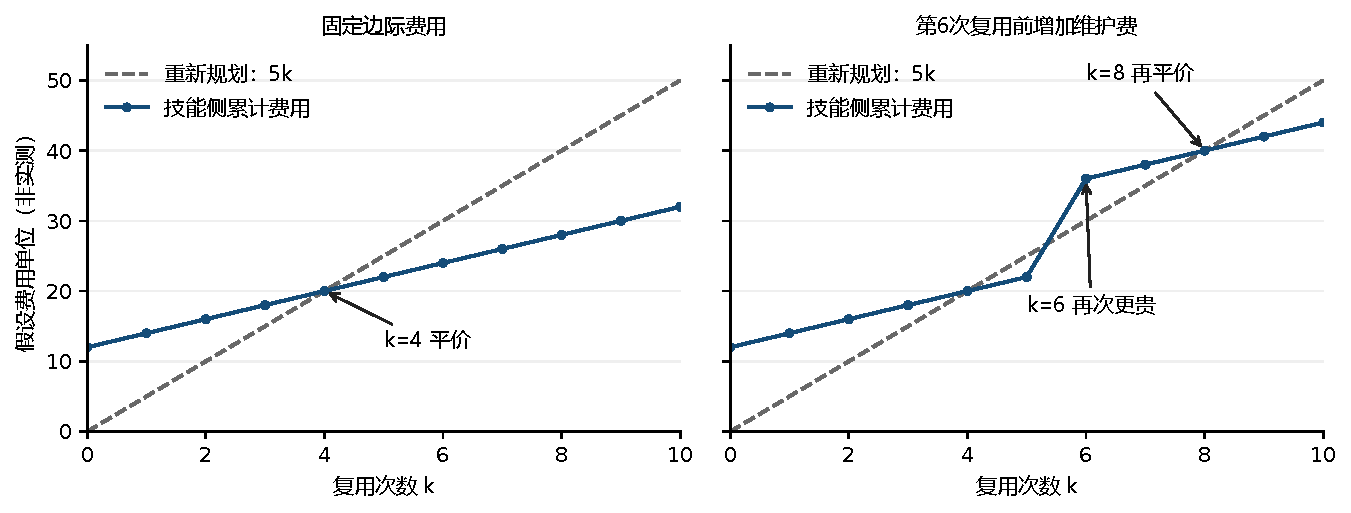
\includegraphics[width=0.98\linewidth]{figures/generated/ch08-cost-teaching.pdf}

\caption{构造的费用模型：左侧固定准备与复用费用在 $k=4$ 平价；右侧第六次前支付一次维护费，费用关系暂时反转，到 $k=8$ 再平价。全部为教学假设，非 E05 实测或拟合，原数组与公式可复算。}
\label{fig:ch08-kstar}
\end{figure}


\subsection{一个能精确复算的教学成本图}

图~\ref{fig:ch08-kstar} 使用明确的\textbf{假设费用单位}。重新规划没有额外准备费用，每次需要五单位；技能准备需要十二单位，每次复用需要两单位。因此两条线为 $5k$ 与 $12+2k$，按式~\ref{eq:ch08-integer-threshold}，最早在\calcnum{$k=4$}时平价，最早在\calcnum{$k=5$}时严格节省。它说明固定成本和边际成本如何共同决定交点，不是对任何真实模型调用价格的拟合。

右图保持同样条件，但假设第六次复用前必须支付十二单位维护费。第五次复用时，技能累计二十二单位，低于重新规划的二十五单位；到第六次，技能累计三十六单位，高于重新规划的三十单位；到第八次又达到四十单位平价。这些都是本书构造条件下的精确计算，原始数组与公式随图保存。

这个例子同时解释了“首次交点”和“以后始终更便宜”的区别。只观察前五次，可能认为技能已经回本；加入后续维护，累计优势却会暂时消失。真实系统的维护时点、费用和失败损失不一定如此规则，因此不能用一条拟合直线替代整个生命周期。若报告一个阈值，应明确它是已观测范围内的首次非正成本差，还是在更强模型假设下推导出的长期阈值。

频率在这里如何进入？如果费用只按调用次数发生，同样十次使用分布在一天或一个月，不改变次数轴上的两条线。若按月需要刷新依赖、资产会过期，或长时间不用后必须重新核验，日历时间才带来额外成本。此时可以写出同时依赖次数和时间的费用，而不能一边沿用纯次数模型，一边声称频率降低必然使次数阈值右移。

\subsection{成功率约束不能从成本线里省掉}

最便宜的策略可能是遇到难题立即停止。若只比较调用费用，它甚至可以击败所有认真实现的技能；对实际任务却没有意义。成本比较应在明确的质量要求下进行，或者并列报告成本与质量，避免把减少有效工作误读成效率。

一种做法是预先规定可以接受的性能损失，再检查技能方案是否满足相应约束；另一种是保留质量与费用两个维度，不把它们合成单一分数。若采用失败惩罚加权总费用，惩罚权重应有任务依据，并做敏感性分析。不能在看到结果后调大某项权重，使偏好的方案刚好成为最优。

E05 v2 的动态组提供了很直接的提醒：来源任务格式失败使其较早停止，调用账可能因此变小，后续又没有有效技能。把这种轨迹压成一个平均费用，会让工程失败看起来像高效策略。完整结果应同时列来源通过、准入、实际读取、首轮成功、额外修复和发布事件，成本线才不会脱离行为过程。

\subsection{平均维护费用可能遮住长尾}

两个技能的平均复用成本相同，失败分布却可能完全不同。一个每次都稍贵，另一个大多数时候很便宜，偶尔需要长时间人工排查或大量模型修复。是否接受后一种模式取决于任务的延迟和恢复要求，不能仅凭均值决定。

实验可以报告费用分布、上分位数或超预算次数，但小样本无法稳定估计很罕见的尾部事件。没有观察到昂贵修复，不等于修复费用为零。对于当前仅少量任务的流程试跑，应直接报告修复路径是否被触发；若没有触发，相关成本和成功率属于未观测，而不是完美表现。

技能退役也有成本。删除一份代码可能很便宜，识别它的所有调用者、迁移依赖、清理旧检索索引和验证替代版本却不一定便宜。生命周期账应允许这些费用出现。若研究只覆盖创建与短期复用，就如实限定范围，不把这一小段累计费用称为长期拥有成本。

\subsection{有缺失费用时，宁可保留区间也不要制造交点}

费用缺失与费用为零是不同状态。一次外部请求超时，应用可能没有收到 usage，但服务端可能已经执行；一次恢复运行只加载任务结果，也可能漏掉之前的构建账。若把这两种情况都填成零，成本较低的一方可能只是记录更不完整。图上的交点越精确，这种误解反而越隐蔽。

若能为缺失费用给出有依据的上下界，可以将总成本写成相应范围，再检查两个方案的范围是否仍然分离。若缺少合理上界，就应明确该格点的完整成本未知，不能通过平均其他任务来伪造一笔已支付费用。估计值可以作为单独的情景分析，必须与记录值分开。

相同问题也出现在时间账里。逐 episode 的耗时相加，不一定等于用户从提交到完成所经历的总时间；并行任务的耗时总和又可能大于墙钟时间。准备环境、构建索引、等待队列和恢复中断，都可能不在模型响应计时内。报告应分别命名累计执行时间与完整流程墙钟，不把现成字段换一个更宽泛的名字。

成本审计应从最小事件向上求和，再与序列、格点和全局汇总核对。同一事件只能计入一次总账，但可以带有多个分析标签，例如属于修复阶段、使用某个模型、服务某个技能。标签用于分组，不应让同一笔费用在总计中重复出现。E05 旧分析将累计复用调用再乘次数，正是没有守住这一层级关系。

记录不完整并不要求丢弃所有数据。已经保存的任务真值、调用次数和错误轨迹仍有价值，只是支持的主张变窄。可以报告部分成本、确定发生的事件和缺失范围，暂缓完整回本判断。这样比覆盖旧记录后补一张完整表更利于后续修复，也更符合本书对历史运行的处理原则。


% ---------- 5. 条件变化 ----------
\section{怎样设计能区分复用与多算力的试验}
\label{sec:ch08-next-design}

技能方案常常同时拥有来源任务、持久代码、额外提示和失败修复，基线却只拿到当前问题。这样的系统比较可以回答“采用整套流程是否值得”，不能单独回答哪一项造成改进。若想归因于代码参考本身，需要为两边对齐起始信息、当前任务预算和其他反馈，或者将额外信息明确作为干预的一部分。

动态技能与静态技能的比较尤其如此。动态臂多一次修复机会，当前任务结果可以因为额外计算改善，后续任务又可能因为新版本改善。E05 新设计将首轮结果和修复结果分开，避免直接改写主结果；但动态修复还可能为未来任务增加有用经验，因此其总预算仍与静态臂不同。描述这一完整策略是合理的，宣称差异只来自“会更新”则需要进一步对照。

可以加入不写持久物、但拥有相同任务内修复预算的对照，帮助区分额外求解与持久更新。也可以让两条策略都完成相同来源构建，再只向其中一条提供代码参考，检查资产可见性的作用。这些设计会改变所回答的问题，不能在一张表里只保留最有利的对照而不说明关系。下一次真实试验需要先冻结设计与预算，再运行。

\subsection{失败修复：当前任务的第二次机会与下次任务的第一份经验}

一个复用任务失败后，可以继续修当前答案，也可以改供下一题使用的持久物。
两个动作发生在同一时刻，却有不同评价对象：前者影响当前任务最终能否完成，后者影响后续任务的起点。
只报最终成功率会把多一次尝试与更好的持久经验混在一起；只报持久写入次数又看不出写入是否经过验证。
实验需要同时保留首次验收、修复验收和版本发布三个事件。

E05 新版把首次验收固定为主结果。
首次失败后，即使修复成功，原来那一格仍然记录失败，另列修复结果和修复成本。
修复通过且满足准入条件时，才用新条目替换旧参考；修复失败则保持原来的有效条目。
如果旧库本来为空，修复失败后仍然为空，不能为了使动态臂``确实发生了更新''而把失败代码硬塞进去。

修订预算必须带着作用范围一起书写。
``每次复用机会允许一次修复''与``整段任务序列允许一次修复''会产生不同的额外调用量。
旧协议采用前一种单位，因此在每次机会重新计数并不自动违反那份文字协议；
本书 v2 主动采用后一种单位，使预算对象成为一个任务族、一个格点、一次重复构成的完整序列。
这是实验设计的改动，不能在旧运行剩余的两块上换上新逻辑，再把全部结果并成同一组。

预算耗尽描述的是\textbf{不再给予修复机会}，不是另一个任务真值。
当前任务仍按实际验收记成功或失败，额外标记``修复被预算拒绝''。
把超预算另立为既非成功也非失败的类别，再从成功率分母中排除，会使失败较多、较早耗尽预算的策略得到不恰当的统计待遇。
完整账本应让读者同时看到：失败多少次、请求修复多少次、准许多少次、修复成功多少次、最终发布多少次。

\subsection{复用格点是否共享同一条前缀}

一种设计从同一份来源技能连续运行后续任务，在第零、第一、第二和第四次复用处读取累计费用。它能直接观察一条生命周期的前缀，但各格点高度相关，后续任务也受前面更新影响。另一种设计为每个格点独立重建技能、独立运行相应长度的序列，格点之间包含来源生成的随机差异。两者都可采用，解释却不同。

E05 新协议采用独立格点：每个任务族、格点和重复构成一条重新建立的序列。因而不同格点的构建费用可能不同，成本曲线不是同一个技能生命周期的连续采样。不能从独立格点的波动直接推出某条技能在第几次发生维护，也不能将较小格点的构建费用替换进较大格点以获得更平滑曲线。

如果目标是估计真实部署的一段连续使用过程，应另外安排共享前缀的任务流，并保留状态演化。若目标是比较不同预期复用长度下的重新部署成本，独立格点更贴近该问题。选择设计时应从使用情景出发，不应因为某种图更好看就混用两者。

\subsection{任务族的重复与独立证据}

同一模板下替换几个常数，确实可以产生不同输入，但不一定提供新的机制覆盖。若所有任务都考察闭区间端点，重复再多也很难说明技能对状态管理或异常契约有效。任务族内重复可以估计当前机制下的随机波动，跨族覆盖则关系到适用范围，两者不能互相替代。

一个小规模试跑更适合回答装置问题：技能是否进入提示、来源失败是否被拒绝、修复预算是否正确扣除、恢复运行是否重复计费。它可以据此发现下一轮值得修复的问题，却不应被迫承担普遍临界次数的证明。把每项运行的用途写清，比让所有运行都输出一个看似完整的命题结论更可靠。

当前v3只有离线验证，沿用的执行路径尚不具备经验证的操作系统隔离；v4仅有受限文件工具草案，没有完整运行器。本版仍缺完整技能依赖图、自动退役和真实接口变更回归数据，也未验证返回语义漂移判据。后续试验需要先完成执行边界与资源记录，再冻结任务独立性、质量约束和比较单位。

\section{条件变化：换环境、换模型、换接口}
\label{sec:ch08-conditions}

\begin{itemize}
  \item \textbf{换环境。}Voyager 在重置的新世界中进行零样本评价（表~\ref{tab:ch08-voyager}）。
        所报迭代数的差距方向一致，证据范围为 \cited{3} 次运行、\cited{4} 个任务。
  \item \textbf{换模型。}原文 GPT-4 版本发现的独特物品数是 GPT-3.5 版本的\cited{5.7}倍（Fig~9），
        而原论文当时报告的 GPT-4 API 价格是 GPT-3.5 的 \cited{15} 倍\cite{voyager-2305}。
        比较带技能库系统的表现与费用时，需要同时报告代码生成模型。
        该对照同时改变技能生成与执行决策，所得差异属于整套系统。固定技能资产的迁移还需要保持资产不变，单独替换读取者。
  \item \textbf{换接口。}高层 API 变化可能造成显式报错或静默的语义失效。
        Voyager 的报告里没有接口版本变更的对照\cite{voyager-2305}；
        2608.03392 把``组件退役''与``回滚成功率与成本''列为应当报告的度量\cite{coding-survey-2608}，
        这是一项评价要求，不能据此概括全部方法都没有相关数值。\textbf{本章尚无接口升级后的真实对照数据。}
  \item \textbf{重复率下降。}复用频率决定需要等待多久，才能累积到某个使用次数。
        在仅按次数计费的固定成本模型中，频率不改变次数轴上的交点；若还存在按时间发生的维护或过期，日历节奏才会进入成本模型。
        若实际使用次数达不到所需阈值，即使技能在每次调用中都有效，也可能无法收回准备费用。
        因此报 $k^{*}$ 时，应同时给出观察时间窗口及实际或预期使用量。
  \item \textbf{技能库增大。}候选池变大而注入条数固定（Voyager 取 \cited{5} 条），
        不能据此预定检索方差必然上升；需要同时观测检索费用、适用候选召回与误调用。相关成本既可能体现为费用，也可能体现为失败。
        因此技能库的规模必须与误用率一起报告，
        单报规模既不能证明收益，也会遗漏检索和维护费用。
  \item \textbf{检索与误调用的代价变化。}        检索要付算力与延迟，误调用一次要付调试与回滚。
        这两笔费用应按实际发生阶段计入，
        若这些费用增加在每次复用上、其他条件固定，就可能提高复用成本，使原交点右移甚至不再出现；一次性费用则改变累计成本的起点，不能都算作斜率。\emph{检索做得更好与技能更划算不是同一件事}——
        检索可能增加计算也可能减少误用，交点变化方向应由两者合计后的实际成本决定。
\end{itemize}

% ---------- 6. 选择原则 ----------
\section{选择原则}
\label{sec:ch08-choice}

\begin{enumerate}
  \item \textbf{把``该不该固化''做成一次带验收的判决，而不是生成的副产品。}
        最小要求是记录：这次固化依据的是哪几次执行，判定者是谁，有没有被反驳过。
  \item \textbf{技能元数据必须含不适用条件。}
        只写适用条件时，库增长可能增加不合适候选；是否提高误用率必须另测，不能预设单调关系。
  \item \textbf{回本点要用成本曲线算，不要用复用次数猜。}
        固化那一次的调用与 token 要计入；$k$ 数的是同一件事的重复次数。
  \item \textbf{被引用者变更时，依赖它的组合技能必须重新验证。}
        版本及依赖记录有助于找出受影响集合，应纳入维护流程。
  \item \textbf{报告技能库收益时，同时报告基础模型与接口版本。}
        少了这两栏，数字无法跨报告比较（见 §\ref{sec:ch08-conditions} 的换模型一项）。
\end{enumerate}

% ---------- 7. 反例 ----------
\begin{pitfallbox}
\textbf{反例一：把``这次跑通了''当成技能成立。}
Voyager 自陈 self-verification 偶尔判错、课程偶尔提出不可达任务、
生成的代码偶尔调用不存在的 API\cite{voyager-2305}。
跑通一次只说明这一次的参数与环境下它能跑，不说明它描述了那件重复发生的事。

\textbf{反例二：把库变大当成能力变大。}
检索固定取 \cited{5} 条\cite{voyager-2305}，库增长后候选集合变化，但仅凭条数不能推出检索方差的方向。
2608.03392 把``组件退役''列为应当报告的度量\cite{coding-survey-2608}，
原论文未给出完整退役对照，本书不据此证明库规模与质量的必然关系。

\textbf{反例三：把换模型后还能跑当成技能可移植。}
GPT-3.5 下发现物品数是 GPT-4 下的 \calcnum{1/5.7}\cite{voyager-2305}。
这是替换代码生成模型后的整套系统对照。评价技能资产的可移植性，还需固定技能版本，并报告两个读取模型各自的无技能库基线。

\textbf{反例四：把复用次数当成回本点。}
回本点是成本线的交点（图~\ref{fig:ch08-kstar}），
Voyager 的成本段没有``回本所需任务数''这一项\cite{voyager-2305}。
用``复用了三次所以值了''来替代成本计算，等于把固定成本那一笔划掉。
\end{pitfallbox}

\section*{习题}
\begin{enumerate}[label=8-\arabic*.,ref=8-\arabic*]
  \item\label{ex:ch08-1} 选一个你正在用的技能库，统计其中有多少条元数据里有``不适用条件''这一项。
        如果没有，估算误用率随库规模的变化需要额外记录什么。
  \item\label{ex:ch08-2} 表~\ref{tab:ch08-voyager} 在相同的最大提示迭代预算下比较有无技能库。
        它已经提供什么证据？若进一步比较包含来源构建费用的总资源效率，还缺哪些记录与对照？
  \item\label{ex:ch08-3} 先用式~\ref{eq:ch08-integer-threshold} 区分平价与严格节省的最早次数，再检查图~\ref{fig:ch08-kstar} 右侧加入的维护费用。
        若维护费用更高或更早发生，请计算哪些格点的成本关系会改变。
  \item\label{ex:ch08-4} 本章说``本章尚无接口升级后的真实对照数据''。
        请设计一个最小实验，使得``接口变化后有多少已入库技能静默失效''这个数可以被测出来。
\end{enumerate}

\section*{常见误解}
\begin{itemize}
  \item \textbf{``代码技能比文本记忆更可靠，因为能跑''。}
        能跑只验收了这一次执行。Voyager 自陈生成的代码偶尔调用不存在的 API\cite{voyager-2305}——
        部分这类错误在执行前可由接口检查发现，不能只依赖最终运行。
  \item \textbf{``技能越多越好''。}
        检索只取 \cited{5} 条\cite{voyager-2305}，多出来的部分不进入上下文，
        它们仍可能影响检索与维护，方向和大小需要测量，不能自动当作成本增加。
  \item \textbf{``消融掉了技能库还更差，说明技能库有用''。}
        在其他条件受控时，这可以提供技能库贡献的证据；但它不足以回答P4：P4 说的是存在临界重复次数，
        需要的是成本曲线，消融给的是有/无的二分对照。
  \item \textbf{``技能库跨任务复用，所以它是通用的''。}
        原文换代码生成模型后发现物品数相差 \cited{5.7} 倍，这不是冻结同一技能库后换读取者的实验\cite{voyager-2305}。
        可复用与可移植是两件事，第 5 章的 E03c 检验的是后者，当前 P3b 仍未判定。
\end{itemize}

\section*{进一步阅读}
\begin{itemize}
  \item \cite{voyager-2305}：本章 Voyager 相关数字的出处，E05数字另有本书原始记录。
        Sec~2.2 与 Fig~4 是技能库结构；Table~2 是表~\ref{tab:ch08-voyager}；
        Sec~3.4 的消融（随机课程 \cited{-93\%}、去 self-verification \cited{-73\%}）与
        Sec~4 的成本段（GPT-4 比 GPT-3.5 贵 \cited{15} 倍）是本章反例一与反例四的来源。
        读它时注意：``回本所需任务数''是未定位项。
  \item \cite{coding-survey-2608}：六类持久演化目标里 skill and tool 的位置（§3，Table~3），
        以及 §5.2 那份把``组件退役''与``回滚成本''列为度量的清单。
        本书使用v3的章节定位；引用时不要把``应当报告''读成``已经报告''。
  \item \cite{ksi-2607}：\texttt{applies\_when} / \texttt{does\_not\_apply\_when} 的出处，
        本章 §\ref{sec:ch08-interface} 把它搬到了技能元数据上。
  \item 本书第 4 章：验证层级四级与六类代码信号的分布，
        \cited{75.4\%} 依赖可执行验证那个数字解释了本章的域边界。
  \item 本书第 5 章：两种拟合目标与 E03c。技能是最容易被写成``拟合到求解器''的一种持久物，
        因为它的正确性常常依赖那个模型会不会写出正确的调用。
\end{itemize}

% chapters/ch09.tex —— 第 9 章
% 体例：具体失败 → 设计问题 → 机制解释 → 对照实验 → 条件变化 → 选择原则
% 数字身份纪律：AFlow 与 ADAS 的数字一律 \cited{}（出处见 source-map 第 9 章各条）；
% 由引用数字算出的量用 \calcnum{}。E06 尚未运行，本章不报告它的任何数字。
\chapter{工作流与多 Agent 结构的演化}
\label{ch09}

\chaptergoal{应该改一个节点，还是改组织这些节点的方式？}
\chapterprops{本章沿信息流解释结构改动，分别计算搜索投入与部署资源，再用相同总预算的多采样对照检查结构增量。E06保留为尚未运行的B级受限设计。}
\chapterfig{图~\ref{fig:ch09-workflow}：三种组织方式及各自的资源账}
\chapterpitfall{把结构变复杂当成找到了更好的结构；把搜索成本排除在比较之外；
把跨模型能用当成跨模型无损}

% ---------- 1. 具体失败 ----------
\begin{failurebox}
AFlow 用 Claude-3.5-sonnet 作为优化器，以 GPT-4o-mini 的执行反馈搜索出的工作流，换用 DeepSeek-V2.5 执行时报告
\cited{0.9390} 的 HumanEval 分数，而 GPT-4o 直接调用是 \cited{0.9389}——
论文报告前者的测试执行费用为后者的 \cited{4.55\%}\cite{aflow-2410}。

两个分数的点估计接近。统计等效需要相应比较证据，费用比也有明确范围。
那个 \cited{4.55\%} 只统计\emph{测试执行 token 按当时模型价格折算的美元费用}。
该实验的 MCTS 最大轮数设为 \cited{20}、每轮把候选工作流在验证集上跑 \cited{5} 次\cite{aflow-2410}，
搜索费用没有进入这张测试执行费用表；未报告部署复用量时，不能说已完成摊销。

同一次比较里还有第二个缺口：
作者列出的基线里已经有多尝试方法（CoT 自一致性 \cited{5} 个答案、
MedPrompt \cited{3} 个答案 \cited{5} 票、Self-Refine、MultiPersona），
但``给一个扁平采样器与结构搜索同等预算、取 best-of-N''这一组对照并未出现\cite{aflow-2410}。
也就是说：\textbf{我们不知道这 \cited{4.55\%} 换来的分数，
是不是同样多的钱用来多采样几次也能拿到。}
\end{failurebox}

\designquestion{判据不是``搜出来的工作流分数更高''，而是：
\textbf{在同等总预算下，把钱花在搜索结构上，是否比花在同一次推理的多采样上更值}。
回答它需要同时保存搜索投入、部署资源和任务结果。}

第7章以指令、示例和上下文为主要对象，第8章讨论可复用的可执行片段。
本章将\emph{节点之间的连接}作为显式搜索对象；程序优化也可能跨越这些边界。
这一层同时允许提示与连接变化，可能增加候选组合和评价负担，
因此也最容易在预算口径上出问题。

% ---------- 2. 机制解释 ----------
\section{工作流的表示：节点、边与算子}
\label{sec:ch09-repr}

AFlow 把一个工作流写成节点序列 $N$ 与用代码表示的边 $E$，
每个节点是一个带提示、温度与格式的模型调用，边决定调用顺序、条件与循环\cite{aflow-2410}。
优化的目标是

\begin{equation}
W^{*}=\arg\max_{W\in\mathcal S} G(W,T),
\label{eq:ch09-aflow}
\end{equation}

其中 $G$ 是工作流 $W$ 在任务 $T$ 上的得分\cite{aflow-2410}。

用代码表示边带来一个直接的后果：顺序、分支、循环、并行与路由
都能被同一个表示装下，不需要为每种结构单独设计一套语法。
ADAS 把这一点推到了头——既然多数编程语言是图灵完备的，
``用代码定义 agent''在理论上能表达任何 agentic system，
包括新的提示、工具用法、工作流及其组合\cite{adas-2408}。

\begin{principlebox}
\textbf{表达能力强不等于搜索得动。}
通用代码表示具有很强的表达能力，但实际工具接口、运行预算与安全限制仍会约束可执行集合，搜索器也仍有先验。
AFlow 因此把搜索交给 MCTS：树的一个节点是\emph{一整个工作流}，
而不是工作流里的一个节点\cite{aflow-2410}。
评估单位随之变成``把整个工作流在验证集上跑一遍''——
提示优化也可能评估整个多模块程序，因此不能预定这里贵一个数量级，费用需要按实际任务和候选结算。
\end{principlebox}

ADAS 给出另一个部件：一个持续增长的 archive。
被发现的 agent 连同它的指标一起入档，元 agent 参考这份档案设计下一个\cite{adas-2408}。
这就是结构搜索里的``经验''——注意它存的是\emph{被评估过的候选}，
是服务于搜索过程的持久状态；它与部署时读取的经验用途不同，是否跨搜索复用取决于设计，不能由名称判定它不持久。

\section{五种结构原语各自承担什么}
\label{sec:ch09-primitives}

用代码表示边的好处是表达能力强，代价是``结构''这个词变得太大。
把它拆开看，本章用五种常见控制原语拆解工作流，不声称穷尽全部结构；它们的功能不同，
也因此带来不同的失败方式。

\begin{table}[htbp]
\centering
\caption{五种结构原语：各自承担的功能、新增的失败方式与必须记录的量}
\label{tab:ch09-primitives}
\begin{tabular}{>{\raggedright\arraybackslash}p{1.6cm}>{\raggedright\arraybackslash}p{3.4cm}>{\raggedright\arraybackslash}p{3.5cm}>{\raggedright\arraybackslash}p{4.0cm}}
\toprule
原语 & 承担的功能 & 新增的失败方式 & 必须记录的量 \\
\midrule
顺序 & 把一个结果喂给下一个节点 & 上游的错误被下游当作事实继续推导 & 每一跳的输入输出对 \\
分支 & 按条件选择不同路径 & 条件错误导致错误路径；无日志时难追查 & 每次判定的条件与选中分支 \\
循环 & 在达到条件前反复修改 & 没有可判定出口时调用数无上界 & 迭代次数与每轮的改动量 \\
并行 & 同一问题取多条可能相关的尝试 & 新增生成与聚合费用；相关错误可能保留 & 路数、每路结果、聚合规则 \\
路由 & 按问题类型分发到不同子流程 & 分发错时错误被归因到被选中的子流程 & 分发判据与命中分布 \\
\bottomrule
\end{tabular}
\end{table}

\begin{sloppypar}
表~\ref{tab:ch09-primitives} 的第二列说明一件容易被说反的事：
\textbf{这些原语改变信息流与计算分配，是否提高任务能力需要对照。}
顺序把不确定性留在下游，分支把它变成一次判定，循环把它换成更多调用，
并行把它摊到多条路上，路由把它交给一次分类。
因此``加了某个结构所以分数上升''这句话缺少一个中间环节：
必须说明是哪一个原语把哪一种不确定性换掉了，以及换来的代价是什么。
\end{sloppypar}

表~\ref{tab:ch09-primitives} 的后两列把失败方式与记录位置对应起来。例如，分支条件选错后，最后答案的零分无法说明问题出在路由还是求解；保存分支判定及下游输入，才能沿调用链定位。质量、执行路径与资源需要一起读。

\subsection{合法结构的约束：搜索空间必须删掉什么}
\label{sec:ch09-legal}

图灵完备的表示能装下任何结构，包括运行不起来的那些。
一个结构搜索器如果不先删掉一部分结构，就会把预算花在证明它们不行上。
下面四条约束分别处理终止、状态、评价与接口，避免无界执行或无法解释的结果：

\begin{enumerate}
  \item \textbf{循环必须有可判定的出口与强制上界。}
        验收结果可触发提前退出，计数器或运行预算还须保证始终未通过时也会停止。
        允许``改到满意为止''等于允许调用数无上界——
        第 \ref{ch02} 章的 episode 预算在这里变成结构层面的预算。
  \item \textbf{并行共享状态必须有明确同步语义。}
        缺少同步时可能出现调度依赖；可以使用隔离副本、事务或明确的合并规则。随机性本身不使配对比较失效，但状态耦合须进入设计与分析。
  \item \textbf{验收器不在结构的可写侧。}
        这是第 \ref{ch01} 章公理一（验证器冻结）在结构层的同一条约束：
        本章固定共同判据；若另行研究评价器更新，旧分差不能直接解释为同尺度改进，应保留共同外部参照。
  \item \textbf{每个节点的输出必须有类型契约。}
        节点可以传文本或结构化对象；解析器能捕获部分形状错误，语义错误仍可能传到下游。
        契约缺失时，失败会被归因到最后一个节点，而真正的起因在上游。
\end{enumerate}

\begin{principlebox}
\textbf{表达能力、合法性检查与搜索效率要分别说明。}
ADAS 与 AFlow 都用代码表示候选。AFlow 提供算子来帮助搜索，但也允许通过 Custom 构造节点，并报告不使用预定义算子的消融；不能把它描述为只允许七种固定结构。预定义接口可以减少部分无效候选，却不保证整个程序一定终止或正确。反过来，通用表示也可以配合运行时预算和校验器。
\end{principlebox}

\subsection{提示优化与结构优化：两个不同的搜索空间}
\label{sec:ch09-space}

\begin{table}[htbp]
\centering
\caption{两类优化的搜索空间与评估代价}
\label{tab:ch09-space}
\begin{tabular}{>{\raggedright\arraybackslash}p{2.8cm}>{\raggedright\arraybackslash}p{5.0cm}>{\raggedright\arraybackslash}p{5.1cm}}
\toprule
 & 提示 / 示例优化（第 7 章） & 结构优化（本章） \\
\midrule
搜索对象 & 模块指令、示例与上下文 & 节点之间的边与算子组合 \\
候选评估 & 可能评估完整多模块程序 & 按完整候选及其路径评估 \\
行为影响 & 可影响本模块及其下游输入 & 可改变可达路径、调用顺序与资源分配 \\
失败形态 & 塌缩、记住题目 & 调用数膨胀、等待时间变长 \\
\bottomrule
\end{tabular}
\end{table}

表~\ref{tab:ch09-space} 最后一行的差别最容易被忽略：
两类优化都可能改变分数、调用数和等待时间。提示可以诱导额外工具调用，结构可以改变答案质量，不能将两种失败形态绝对分开。
开头的费用案例需要按同样的原则分解。

AFlow 的算子集合给出结构搜索的原子：
Generate、Format、Review \& Revise、Ensemble、Test、Programmer、Custom\cite{aflow-2410}。
算子可以封装多个调用或条件执行，增加一个算子不等于固定增加一次模型调用。

\section{候选工作流的生成与局部修改}
\label{sec:ch09-search}

AFlow 的一轮迭代是四步：Select（软混合概率选择）、
Expand（由模型优化器改提示与代码边生成子工作流）、
Evaluate（验证集上测 \cited{5} 次）、
Backpropagate（记录性能与这一改的成败）；
终止条件是最优若干候选连续若干轮无改进，或总轮数到 \cited{20}\cite{aflow-2410}。

\begin{sloppypar}
\textbf{先保留原文中的一个参数歧义。}
正文式(3)说明采用 $\lambda=\cited{0.2}$、$\alpha=\cited{0.4}$，但附录 A.6 详细算法第36行写作 $\lambda=\cited{0.4}$、$\alpha=\cited{0.2}$\cite{aflow-2410}。前者控制均匀探索权重，后者控制分数对选择概率的影响，交换它们不是无关紧要的排版变化。固定公开实现又采用另一组默认值，见下一小节。论文说明、代码默认项和历史运行有效配置需要分别记录，原表参数尚缺检查点或运行配置的直接绑定。

\textbf{Backpropagate 这一步值得单独看。}
它把候选相对父候选的表现及修改记录写回树里，形成关于修改效果的反馈。
它与第 6 章的准入判决、第 8 章的入库判决是同一类东西：
都是``这次更新值不值得''的显式记录。
这份经验主要用于搜索选择；原文没有据此规定搜索结束必须销毁，跨搜索复用需要额外设计和验证。
\end{sloppypar}

\subsection{分数变换也属于选择参数}
\label{sec:ch09-score-scale}

固定公开提交的选择函数默认 $\alpha=\cited{0.2}$、$\lambda=\cited{0.3}$，先将读入的得分乘以\cited{100}，再计算指数权重并与均匀分布混合\cite{aflow-code-2025}。对非空且得分有限的候选集，令 $0\le\lambda\le1$，用原始得分 $s_i$ 表示这条路径，其概率为
\begin{equation}
 p_i=\frac{\lambda}{n}+(1-\lambda)
 \frac{\exp(\alpha\widetilde s_i)}
      {\sum_{j=1}^{n}\exp(\alpha\widetilde s_j)},
 \qquad \widetilde s_i=100s_i.
 \label{eq:ch09-reference-selection}
\end{equation}
实现先减去最大分数再取指数，得到相同概率并改善数值稳定性。均匀项只在已经进入当前父候选集合的工作流之间分配，不表示在整个代码搜索空间中均匀抽样。

以本书构造的两个原始得分\calcnum{0.80}、\calcnum{0.81}为例，代入这份参考实现的默认值，较高分者被抽到的概率约为\calcnum{0.5349}；若遗漏乘以百的步骤，就会算成约\calcnum{0.5003}。这两个数是公式计算，不是一次搜索实测。系数只有连同分数单位和变换一起保存，才能说明选择偏好。

这份仓库说明包含从 MetaGPT 迁移后的实现边界\cite{aflow-code-2025}。上述默认值能够定位公开脚本的行为，尚不能替代原论文两组参数所对应的历史运行配置。复现记录应保留原始得分、变换、候选集合与最终抽样概率。

\subsection{搜索看过哪些题，决定它学到了什么}
\label{sec:ch09-validationselection}

AFlow 的初始化还有一个与预算和泛化同时相关的细节。原文说明，先用固定随机种子\cited{42}把数据划分为\cited{20\%}验证集与\cited{80\%}测试集；随后在验证集上将空白模板运行\cited{5}次，选出得分方差较高的题目作为最终验证子集\cite{aflow-2410}。这一步发生在工作流迭代之前，并且使用模型反馈决定后续搜索主要看哪些题。

高方差题可能更有区分力：对于始终答对或始终答错的题，一次小结构修改可能很难在有限重复中显示差别；处在边界的题则可能更敏感。但这也改变了搜索所见任务的分布。最终验证均值代表的是筛选后的子集，不能不加说明地当成原验证分布的无偏估计。独立测试仍可评价选中结构在预定测试范围内的表现，前提是测试未再被拿来反复挑选结构。

这项筛选不是因为使用了反馈就必然构成泄漏。关键在于反馈属于哪一个分区、在哪个决策中使用，以及最终主张针对哪个范围。训练或验证数据用于选择候选，本来就是搜索的一部分；把测试结果也拿来选赢家后仍称其为未参与选择的最终检验，才混淆了角色。ADAS 按来源测试表现挑选转移候选的例子，正说明同一个名字为“测试”的集合可能在流程中承担了选择作用\cite{adas-2408}。

初始化的五次运行也要计入搜索成本。若最终报告只从第一轮候选生成开始记账，选题本身就被漏掉。类似地，为设定停止轮数、比较提示模板或调节选择概率而做的探索，都可能消耗资源；它们是否进入当前方法的完整成本，应按预先定义的研究与部署范围说明。没有必要把无法恢复的历史探索硬凑成精确数字，但应保留这部分为未计费用，而不是宣称全部搜索成本已知。

自适应选题还会影响候选之间的可比性。若每个候选都在不同的“最有区分力”题集上评价，均值差异同时包含了结构变化和题目变化。可以固定一份共同评价子集，也可以设计有明确估计方法的自适应分配，但不能简单比较不同题集的原始均分后宣布后者更优。评价记录至少需要保留逐题标识，以便事后发现覆盖差异。

近期预印本中的 EvalAlloc 将搜索反馈与候选确认分成两个阶段\cite{evalalloc-2610}。它先在 SEARCH 题集上完整评价预热候选，建立共享的高信息量题目核心与共同评分参照。随后用稀疏观察为进化搜索提供反馈，搜索期间保持题目参数与评分参照固定。搜索结束后，对有效候选逐轮扩大共享的评价题目前缀并淘汰候选，复用已有逐题结果，只补跑缺失项。进入最后一轮的候选补齐全部 SEARCH 观测后，再按实际结果选出最终程序。这套协议中的 SEARCH 同时用于进化与最终候选选择，DEV 仅作审计，TEST 只评价选出的程序。其预算分配结论仍受所用框架、任务与评价单元约束。

重复评价的作用同样有限。同一份验证集上运行五次，可以观察采样波动，却不能凭此创造五份独立任务分布。若某个候选在这份固定集合上具有特有优势，多次重复仍会保留这种优势。报告时应区分任务抽样的不确定性、模型采样的不确定性和搜索选择的不确定性；只对最终候选的五个运行均值求区间，无法自动覆盖整个自适应搜索过程的选择影响。

档案可以帮助保留这些条件。一个可复用的搜索条目不应只有“结构甲得分最高”，还应写明它在哪个验证版本、哪一批题、什么后端和预算下被选中。再次搜索时，档案中的失败可能提示接口风险，也可能只是旧题分布的局部结果。让新搜索者读取带范围的记录，才有机会使用历史信息而不把旧偏差不断放大。

\section{多 Agent 的角色、通信与协作结构}
\label{sec:ch09-multi}

上面的算子换个说法就是角色：Review \& Revise 是一个评审者，
Ensemble 聚合多个候选，候选生成是否并行要看执行代码，Programmer 是一个会写代码的节点。
在本章采用的表示中，可以把多 Agent 协作展开为工作流：
角色对应节点，通信对应边。这是分析信息流的方法，不要求所有多 Agent 系统都采用预先固定的角色图。

\begin{table}[htbp]
\centering
\caption{AFlow 在六个基准上的整体结果（GPT-4o-mini 执行，原论文 Table~1）}
\label{tab:ch09-aflow}
\begin{tabular}{>{\raggedright\arraybackslash}p{2.4cm}cccccc}
\toprule
 & HotpotQA & DROP & HumanEval & MBPP & GSM8K & MATH \\
\midrule
AFlow & \cited{73.5} & \cited{80.6} & \cited{94.7} & \cited{83.4} & \cited{93.5} & \cited{56.2} \\
\bottomrule
\end{tabular}

\vspace{2mm}
\begin{footnotesize}
数字身份为[引用]，来自原论文 Table~1\cite{aflow-2410}。每种方法测试 \cited{3} 次后取均值。
前两项为 F1，中间两项为 pass@1，后两项为解题率，数值沿用原表的显示尺度。六基准等权平均为 \cited{80.3}。
原文报告相对最强手工基线与 ADAS 的相对提升约为 \cited{5.7\%} 与 \cited{19.5\%}，不是百分点；按表中均值相减分别为 \calcnum{4.3} 与 \calcnum{13.1} 个分数点。
这些数值保留原论文的报告身份。比较工作流的资源效率，还需并列报告调用数与等待时间。
\end{footnotesize}
\end{table}

表~\ref{tab:ch09-aflow}提供了整体质量比较。
它能支持的说法是``在这六个基准上，搜出来的工作流分数更高''；
它不能支持``这些分数是用更少的资源拿到的''——
因为那张表没有资源这一栏。

% figures/ch09-workflow.tex —— 第 9 章核心图（全书引用入口）
% 用法：在 book/chapters/ch09.tex 中 % figures/ch09-workflow.tex —— 第 9 章核心图（全书引用入口）
% 用法：在 book/chapters/ch09.tex 中 \input{figures/ch09-workflow}
% 图主体在 ch09-workflow-body.tex，便于单独编译与复用。
\begin{figure}[htbp]
\centering
\input{figures/ch09-workflow-body}
\caption{顺序、带评审与并行集成的控制流示意。图中节点和分支不同，具体调用量、时延与质量需按实现测量；并行不保证等待时间不变，评审也不保证纠错。即使最终分数相同，执行过程与资源账仍可能不同。}
\label{fig:ch09-workflow}
\end{figure}

% 图主体在 ch09-workflow-body.tex，便于单独编译与复用。
\begin{figure}[htbp]
\centering
% Three full-size panels; no transform-shape reduction.
\begin{tikzpicture}[
 nd/.style={draw,rounded corners=2pt,text width=18mm,minimum height=8mm,align=center,font=\small},
 io/.style={nd,fill=gray!10},
 arrow/.style={-{Stealth[length=1.8mm]},thick},
 note/.style={font=\small,align=left,text width=43mm}
]
\node[font=\bfseries\small] at (0,1) {顺序};
\node[io] (s1) at (0,0) {生成};
\node[nd] (s2) at (0,-1.2) {求解};
\node[io] (s3) at (0,-2.4) {输出};
\draw[arrow] (s1)--(s2);\draw[arrow] (s2)--(s3);
\node[note,anchor=north] at (0,-3.2) {按实际调用与\\执行事件记账。\\等待时间沿串行路径累加。};
\node[font=\bfseries\small] at (5,1) {带评审};
\node[io] (r1) at (5,0) {生成与求解};
\node[nd,fill=orange!12] (r2) at (5,-1.2) {评审};
\node[nd] (r3) at (6.1,-2.4) {修正};
\node[io] (r4) at (5,-3.6) {输出};
\draw[arrow] (r1)--(r2);\draw[arrow] (r2)--(r3);
\draw[arrow] (r3)--(r4);\draw[arrow] (r2.west)--++(-1.2,0)|-(r4.west);
\node[note,anchor=north] at (5,-4.4) {评审与修正分别计费。\\时间取决于实际返回分支。};
\node[font=\bfseries\small] at (10,1) {并行集成};
\node[io] (p0) at (10,0) {输入};
\node[nd,fill=blue!9] (p1) at (8.8,-1.5) {求解甲};
\node[nd,fill=blue!9] (p2) at (11.2,-1.5) {求解乙};
\node[io] (p3) at (10,-3) {聚合};
\draw[arrow] (p0)--(p1);\draw[arrow] (p0)--(p2);
\draw[arrow] (p1)--(p3);\draw[arrow] (p2)--(p3);
\node[note,anchor=north] at (10,-3.8) {各路与聚合均计费。\\等待受并发和排队影响。\\质量取决于错误相关性。};
\end{tikzpicture}

\caption{顺序、带评审与并行集成的控制流示意。图中节点和分支不同，具体调用量、时延与质量需按实现测量；并行不保证等待时间不变，评审也不保证纠错。即使最终分数相同，执行过程与资源账仍可能不同。}
\label{fig:ch09-workflow}
\end{figure}


图~\ref{fig:ch09-workflow} 把缺的那一栏画出来：
三种组织方式即使拿到同一个分数，
它们的调用数与等待时间仍可能不同。
只看分数时，三者不可区分。


\subsection{多角色的增量来自信息，而不来自称呼}
\label{sec:ch09-roleinformation}

给同一个模型分别设置“专家”“反对者”“裁判”三个角色，可能改变它生成的内容，但角色名本身不提供新的观测。若所有角色都读到同一份错误检索材料，又不能访问其他来源，它们很可能围绕错误前提进行精致讨论。这里不需要假定它们总是相关，也不需要否定角色提示的作用；只需要把声称的机制说清楚：增加的是表达视角、独立采样、额外工具，还是有来源的外部证据。

一个反对者如果能够运行独立测试，就多了一条与求解者解释不同的检查通道；如果只能要求“再仔细想想”，则主要增加一次模型推理。二者都可能有用，成本与失败方式却不同。前者可能受测试覆盖不足限制，后者可能沿用同样的错误前提。评价时可以固定角色提示只改变信息来源，也可以固定信息来源只改变分工，从而分别考察哪一项带来可重复的增量。

通信内容也不宜只按长度理解。两个节点各收到一千字，信息可能完全不同：一份包含原始测试输出，另一份只有上游的结论摘要。摘要可以降低成本，却可能删除异常条件、冲突证据或版本标识。若使用摘要结构与直接共享原始轨迹的结构比较，应同时保存原文与摘要，说明哪些字段被保留，而非只报告 token 节省。信息损失未必有害，关键是它是否改变了任务需要的判断依据。

对抗式分工还有一个常见误区：让批评者必须找出错误。这样的提示可能提高问题发现率，也可能鼓励它把正确答案改坏。比较应同时观察错误候选被纠正、正确候选被破坏两个方向。在只保存“批评成功案例”的档案中，后一个方向很容易消失。若任务对误改代价很高，结构可能需要把建议与实际修改分开，再要求一个可执行条件支持修改。

协作结构的消融则需要考虑接口重连。删掉一个评审节点后，直接把它的输入传给下游，可能改变格式；如果删掉的节点同时完成格式转换，分数下降未必来自失去评审能力。较清楚的设计是保留必要的确定性格式转换，只移除要研究的判断功能。反过来，若研究的问题就是整个复合节点是否值得保留，那么连同转换一起删除也合理，但应按复合干预解释结果。

有些结构只在少数任务上被触发。比如困难路由仅服务罕见长题，整体均分上的作用可能很小，却能改变那一类任务的完成率。报告全量结果的同时，可以给预先定义的类别结果；不能只在看到收益后挑一个有利子组。实际触发率、路由失败率和后备路径成本一起记录，才能解释某个角色为什么在多数题上看不见，却仍然有部署价值。

还要注意部件之间的相互作用。假设检查者输出一份精确错误日志，修订者才会据此有效修改；单独增加检查者而不使用日志，最终答案可能不变，单独增加修订者而不给日志，也可能无效。两者合用却可能产生增量。这里的四种配置分别是都无、仅检查、仅修订、检查加修订，能够帮助识别“合用效果是否不同于各自效果相加”。这是一种比较设计，不是本书已观测到的模型结果。

若以四种配置的质量均值记为 $Q_{00},Q_{10},Q_{01},Q_{11}$，可考察交互差 $I=Q_{11}-Q_{10}-Q_{01}+Q_{00}$。非零点值本身仍需不确定性分析；即使得到可靠差异，也只描述当前尺度上的交互，不能直接推断内部认知机制。各配置的资源也不同，应同时记录，避免把额外调用带来的收益全部归为部件协同。

反过来，从完整结构里分别删除一个部件，只回答该部件在其他部件仍然存在时的条件贡献。它没有覆盖“两个部件一起删除后是否可以换一种简单策略”的问题。若工作流有强互补或冗余，逐项消融就不足以给每个节点分配一个唯一功劳值。可以依据机制挑选少量联合消融，而不必穷举所有组合；选择依据和未覆盖范围需要写清楚。

失败路径也可能需要联合检查。正常答案不触发后备路由时，删除后备节点看不到质量变化；这不能证明节点无用。可在隔离环境下构造服务超时或格式错误，检查后备行为是否符合协议。这种故障注入测量的是工程恢复，不应与自然任务的成功率混在同一分母，也不能将人为制造的高故障率当成真实服务故障率。

最终，是否增加一个角色可以落实为很具体的问题：它得到什么此前没有的信息，它能作什么此前不能作的检查，它的输出会改变哪个决定，删除它之后哪些条件保持相同。若这些问题答不清，继续增加角色很可能只增加解释上的复杂度。若答得清，即使结构很简单，也已经具备了被验证和被改进的起点。

\section{从 AFlow 示例还原工作流}
\label{sec:ch09-codecase}

AFlow 的 GSM8K 案例适合练习如何读工作流，因为它把候选代码与搜索路径放在了相邻图中。原论文 Figure~5(B) 展示的程序先生成 \cited{5} 个候选答案，再执行集成，最后调用 Programmer 检查集成结果；如果检查返回的输出非空，就采用该输出，否则保留集成结果\cite{aflow-2410}。这段程序包含生成、汇总、检查和后备返回，读者很容易将它脑补成“多路并行求解后由验证器挑出正确答案”。原代码支持的事实比这句话窄。

下面是依据v4 Figure~5(B)独立改写的最小伪代码。它保留调用顺序与返回条件，省略类定义、提示常量及成本对象；不是原实现摘录，也不是可直接复现实验的代码。

\noindent\begin{minipage}{\linewidth}
\begin{lstlisting}[language=Python,caption={AFlow GSM8K示例的控制流教学改写},label={lst:ch09-aflow},firstnumber=1]
async def solve(problem):
    answers = []
    for attempt in range(5):
        answer = await generate(problem)
        answers.append(answer)
    combined = await ensemble(problem, answers)
    checked_output = await programmer(problem, combined)
    if checked_output:
        return checked_output
    return combined
\end{lstlisting}
\end{minipage}

第3--5行逐个等待五次生成，第6行等待集成，第7行才开始Programmer检查。若第8行条件为真，第9行返回检查输出；否则落到第10行。顶层最多显示七次算子入口，底层请求数仍需打开各算子的实现核对。第8行仅测试输出非空，没有读取标准答案，也没有证明正确。

首先，生成循环在每一次迭代中等待当前调用结束，然后才进入下一次。函数采用异步语法，不等于循环里的请求已经同时发出。若外部服务内部另有调度，那是另一个执行层；图中这段调用方代码本身没有把多个生成请求并发派发出去。因此，在分析该代码的关键路径时，候选生成时长应按这段顺序相加，不能直接取最慢候选的一次耗时。把它重写成真正并发的版本可以成为工程优化，但应记录这是本书提出的改写，不应说论文原本已获得相应的时延收益。

其次，集成收到多个回答，并不等于它掌握了正确标签。固定公开实现中的 ScEnsemble 让模型返回候选编号，再返回对应候选的原文；Programmer 则另行生成代码并尝试执行\cite{aflow-code-2025}。选择已有答案与生成新检查是两种不同的责任。若几个候选沿用相同错误前提，聚合步骤可能只是在几种表达里选出最一致的错误。本例的 Programmer 又接收原题和集成分析，提供了一种可执行检查路径；它究竟调用了多少次模型、执行了几次代码、怎样处理错误，取决于算子的内部实现。顶层出现一次算子调用，只能说明有一次入口调用，不能替代底层模型请求清单。

最后，图中返回分支检验的是输出是否非空。原文 Appendix~A.4 展示的 Programmer 在连续执行失败后，返回的输出是字符串 \texttt{error}\cite{aflow-2410}。若按这两段展示代码直接组合，这个非空字符串也会进入采用分支。这个接口例子说明，执行状态与结果值需要分别传递，错误回执不能靠“是否有文字”识别。本书据此指出展示接口的组合风险，没有重建原实验中错误采用的发生次数。轨迹仍需保留检查状态、实际返回分支与最终任务验收。

\begin{principlebox}
\textbf{角色名说明设计意图，控制流说明实际行为。}
“评审者”可能只有一次无标签的模型判断；“并行求解”可能写成逐次等待；“验证通过”可能实际只是非空检查。分析一个工作流时，应从入口逐步列出等待关系、分支条件与算子内部调用，再给它贴机制标签。论文的流程图、示例代码与运行日志分别提供不同层级的证据，三者不能互相代填。
\end{principlebox}

论文 Figure~6 还展示了搜索如何在增加算子和修改提示之间交替前进。正文讨论的失败尝试包括一轮直接改写答案的评审，以及一轮过度强调题目中折扣信息的重述\cite{aflow-2410}。这些记录有助于理解搜索的具体动作，却不能把某一次分数下降全部归因于“评审有害”或“重述有害”。候选改变的是某个接口、某段提示和某条路径，验证集规模、采样波动及选取规则都影响观测差异。可靠的归因应回到保存的父子版本，并在同一组题上比较它们，而不是从搜索树上挑一条漂亮的上升曲线。

这也解释了为什么失败候选仍有保存价值。它可能暴露一个格式契约缺失，可能说明当前求解器不适合某种检查方式，也可能只是估计不够精确。若档案只保留最终赢家，后续搜索者无法分辨这些情况，只能重复尝试。若把失败候选写成“永远禁止此类结构”，又会把局部观测误升格成普遍规则。更可用的档案记录的是候选版本、改动描述、评价题目、逐题反馈和成本范围，随后由新的证据决定是否复用。停止规则同样需要这些记录：只看保留版本的最高分曲线，会把被拒候选隐藏起来。第\ref{sec:ch13-stop-output}节进一步区分停止搜索与选择交付版本；这不是AFlow原实验已经采用的附加规则。

\subsection{先画出值怎样流动，再给节点命名}
\label{sec:ch09-contractcase}

设想一个教学工作流：求解者读取编程题，生成候选程序；检查者运行公开样例；修订者根据错误修改程序；汇总者交付最终文件。这里没有本书新增的模型结果，只讨论这一设计能否被明确执行。若节点之间只传一段自然语言，“运行通过”可能指语法检查通过，也可能指公开样例通过；下游无法知道这一结论针对哪一个文件版本。即便四个角色各自按照提示认真工作，信息的歧义仍可能让整个流程出错。

因此，边上至少要传递三个不同对象：候选工件的版本、检查事件的状态，以及该事件实际支持的结论。程序版本应由内容或不可变标识确定，检查事件应记录命令、退出状态和输出，结论则注明覆盖的题目范围。公开样例全部通过，可以被表述为“该版本通过了这些样例”，不能直接压缩成“代码正确”。若下一节点又修改了文件，旧检查结果仍属于旧版本，不应自动附着到新版本上。

这个例子说明，类型契约不能只停留在“输入为字符串、输出为字符串”。较有用的契约还包含状态。检查者可能返回通过、失败、超时、工具不可用，或输出不能解析。将后三项全部编码为失败，会把运行环境问题混入算法质量；将它们编码为通过，则会放行没有证据的候选。执行层可以依据任务需要选择重试或后备路径，但证据层应保存原来的区别。下一节点收到的既是一个值，也是对这个值能否使用的限定。

错误还可能发生在边的另一端。假设修订者收到的是候选版本甲的失败日志，却在版本乙上继续修改。日志文字本身完全真实，仍然可能把修订方向带偏。只核对“是否有错误信息”不能发现这种问题；必须核对日志与候选之间的绑定关系。工作流图中的一条箭头因而不只是通信通道，也是对应关系：谁产生了这一观察，它描述哪个对象，接收者要用它作哪一个决定。

在设计接口时，可以把证据放在独立字段，把自然语言解释放在另一个字段。后者便于模型理解原因，却不能覆盖前者。若解释说“全部测试通过”，事件字段却记录超时，运行器应暴露冲突，而非取听起来更合理的一项。若解释无法由事件推出，可以保留为待验证假说。这样做并不会使模型推理自动正确，但能避免不同性质的信息在跨节点传递时被悄悄升级。

接口也需要注明允许修改的对象。一个评审节点可能只允许提出建议，另一个修订节点才有权写入文件；流程图中都画成一个方框，并不能说明权限相同。若评审者在检查前改了候选，原本计划测量的对象已经改变。若汇总者为了“润色”又重写最终代码，前面通过检查的工件可能根本没有被交付。最终返回应明确指向已验收的版本；需要另作修改时，就开启新的候选与检查记录。

这些要求使工作流从一张角色图变成可执行协议。角色名称仍然有帮助，它向读者解释分工；但真正决定可复核性的，是每条边携带的信息、版本和使用条件。AFlow 的非空返回条件就是一个小例子：只有读出这个条件，才能知道图中的检查者实际控制了哪一个决定\cite{aflow-2410}。没有这一步，再复杂的角色描述也不足以解释最终答案从哪里来。

\section{迁移表中一个容易漏掉的选择条件}
\label{sec:ch09-transferselection}

ADAS 的跨模型 ARC 实验并非随机抽取发现的全部结构。原文说明，它先根据 GPT-3.5 上的测试准确率选取表现最好的 \cited{3} 个候选，再把这些候选交给其他模型执行\cite{adas-2408}。这使读者能够考察选中结构在新模型上的表现，却也限定了结论的对象：结论针对这批按来源表现筛选的候选，不能直接推广为搜索产物普遍可迁移。来源测试集已经参与选取，因而也不再承担“完全未参与选择的最终来源评估”这一角色。

Table~3 的逐项比较比“迁移后一致超过基线”的概括更有信息。以 Structured Feedback and Ensemble Agent 为例，Claude-Haiku 上的点估计是 \cited{5.0}，同列 Self-Refine 是 \cited{6.3}；Claude-Sonnet 上分别为 \cited{38.7} 与 \cited{39.3}\cite{adas-2408}。这些点估计不能支持该候选在每个接收模型上均优于最强手工基线。其他候选在相应列可能更高，这支持“存在表现更好的候选”这一较窄陈述。这里也不能仅凭两条单独区间重叠与否宣布差异显著，需要与比较设计相符的差异估计。

迁移审计因而至少有两个不同的分母。一个是选中的候选数量，回答选中后有多少在接收方有效；另一个是搜索生成的全部候选数量，回答整个搜索过程发现可迁移资产的效率。只给前者，无法推断后者。若为了寻找迁移最强的结构又反复查看目标测试结果，目标测试集也会进入选择循环。应再保留一个未用于挑选的评价范围，或把结果明确标成探索性比较。

部署决策还要补上重新适配的费用。沿用来源结构、只调整接口、重新搜索，是三个不同的处理。沿用结构可能省去搜索但损失部分质量；重新搜索可能提高质量却耗时更长；调整接口则需要界定哪些改动仍算迁移，哪些已经改变结构。没有统一的定义，就会把一次重写包装成一次无损复用。第~\ref{ch08} 章对技能版本和依赖的要求，在这里同样适用于工作流版本与模型接口。

本书 E06 的原型尚未运行。本节是对公开论文和代码图的核验，不是本书的新实验。下一步若实现 E06，应先保留候选代码、算子实现和请求清单，再讨论结构是否值得搜索；否则即便得到了一个分数，也无法回答本章最初提出的预算问题。

\section{在质量、调用数与等待时间之间选择}
\label{sec:ch09-tradeoff}

三个量要分开报，因为它们不能互相换算：
\begin{itemize}
  \item \textbf{质量}：分数或准确率。单独报告它不能解释资源代价。
  \item \textbf{调用与token}：共同影响费用；单靠调用数不能确定账单，并行也可能增加等待。
  \item \textbf{等待时间}：决定能不能上线。串行评审不增加并行度，但拉长关键路径。
\end{itemize}

AFlow 的该成本图将测试 token 用量按模型价格折算\cite{aflow-2410}，
因此第二项只有一部分进了账，第三项没有进账，
而\emph{搜索本身}的成本没有包含在此测试费用比较中。
这些口径仍不足以独立证明``结构搜索比多采样划算''这一更窄结论——
E06 要补的就是这个对照。

% ---------- 5. 条件变化 ----------
\subsection{一次逻辑调用可能发生多少次实际请求}
\label{sec:ch09-occurrences}

对工作流计费时，计数对象应是发生过的调用事件，而不是图上画出的节点。设一个候选生成节点在循环里被调用多次，每次调用又可能因网络故障重试；图上仍然只有一个节点，服务端却可能收到多次请求。相反，一个节点可能命中本地缓存而不发出新请求。静态节点数只能描述结构规模，不能直接作为资源消耗。

可以为每次事件保存节点标识、所在迭代、父事件、逻辑请求编号和网络尝试编号。父事件帮助重建调用关系，逻辑请求编号把同一次决策的重试归在一起，网络尝试编号则保留实际派发次数。某次尝试没有收到响应，不代表它在服务端没有执行或没有费用。已知 token、请求次数、未知费用要分别保存；不能因为返回字段缺失就给它填零。

教学设计中，设首轮生成消耗一次逻辑模型调用，每轮评审一次，未通过时修订一次，最多允许两次修订。即使把生成、评审、修订各画成一个节点，最坏路径仍然是生成、评审、修订、评审、修订、评审，合计\calcnum{6}次逻辑调用。若每个逻辑调用最多允许\calcnum{3}次网络尝试，派发上界就是\calcnum{18}次。这里的数字来自规定的控制流，不是模型实测；若算子内部还有未计入的模型检查，上界就必须重新计算。

这个上界还有一个容易漏掉的前提：重试的层级已经统一。若外层允许三次尝试，而客户端内部每次也允许三次，最坏会变成每个逻辑调用九次派发。业务代码看见的“调用了一次客户端”并不等于服务端只收到一次请求。本书新版 E11、E12 的做法是关闭所用后端的内部重试，由外层记录每一次尝试；它解决的是当前实验的计账问题，不代表所有部署环境已经具有这一保证。

循环预算应与请求预算共同使用。只限制修订次数，无法限制一个修订节点内部再开一个无界循环；只限制模型调用，无法限制一次工具执行无限等待。实际运行需要分别说明模型请求、工具步骤、等待时间和输出规模的约束。某些约束可以在派发前检查，另一些只能在完成后得知。例如，不知道下一次真实输出长度时，事前的 token 估计不等于已实现的精确费用硬上限。

预算耗尽后的行为也属于结构定义。一个流程可以返回最后一个已检查版本，可以返回明确的未完成状态，也可以保存现场后终止。它不能在最后一刻绕过预算再请一个模型“总结一下”，然后把总结调用从账上删除。若最终答案来自尚未验收的版本，应清楚标记；如果直接把未完成序列按失败纳入成功率，应事先说明这是业务评价口径，而非运行器无意填出来的默认值。

这类规定看上去属于执行细节，却会改变搜索偏好。一个经常触发重试的结构，按成功返回计费时可能显得很便宜；一个擅长用超长上下文减少调用次数的结构，在只看调用数时可能显得最优。搜索器会利用评价口径中的缺口，无须具有欺骗意图。把事件账写完整，才能让“更好的结构”对应到真正要优化的资源条件。

在各支路均须完成、聚合随后开始，且节点耗时按同一种执行资源计量的条件下，不能直接把节点耗时之和当成并行段等待时间。设并行段有 $m$ 条支路，
第 $j$ 支的节点耗时为 $t_{j,i}$，聚合耗时为 $t_{\mathrm{agg}}$，
并发上限为 $c$，则该段的等待时间不可能短于

\begin{equation}
T_{\mathrm{par}} \;\geq\;
\max\Bigl(\;\max_{j}\sum_{i} t_{j,i},\;\; \frac{1}{c}\sum_{j}\sum_{i} t_{j,i}\Bigr)
\;+\; t_{\mathrm{agg}},
\label{eq:ch09-latency}
\end{equation}

这是上述资源与依赖假设下的下界；缓存、提前退出或异构资源改变工作量时，须重新建立模型。
\textbf{并发充分时最长支路提供约束，串行时总工作量提供约束；一般并发条件下，下界不保证可达}。
在单资源串行、无额外等待的理想条件下，工作时间确实退化为各支路节点耗时之和；并发充分时则由最长支路约束。
把并行支路的耗时相加后直接称作用户等待时间，
混淆的是累计执行耗时与端到端墙钟；它们也都不是调用次数。

\subsection{把并行下界与可以达到的时延分开}
\label{sec:ch09-scheduling}

式~\eqref{eq:ch09-latency} 给出的下界有两个来源：一条有依赖的支路必须等前一步结束，总工作量也必须被有限资源执行完。这两个条件都成立，不表示取二者较大值就一定能安排出那样快的调度。任务是否可切分、服务是否同时可用、某些节点是否争用同一个资源，都会使实际时间更长。

考虑三个互不依赖、不可中断的教学调用，每个都占用同类资源\calcnum{2}个时间单位，并发上限为\calcnum{2}。最长支路为\calcnum{2}，总量除以并发为\calcnum{3}，所以公式下界为\calcnum{3}。实际只能先执行两个调用，第三个等其中一个结束后开始，最早在\calcnum{4}结束。聚合若再占用一个时间单位，最终为\calcnum{5}，而不是由下界误算出的\calcnum{4}。这不是公式失效，而是把必要条件当成了可达方案。

若调用时长不同，派发顺序也可能改变结果。设三个不可中断调用耗时依次为\calcnum{3}、\calcnum{2}、\calcnum{2}，资源仍为两份。先派发两个短调用，再派发长调用，全部完成需\calcnum{5}；先派发长调用和一个短调用，再补另一短调用，只需\calcnum{4}。这组数字是确定性排程演示，不预测真实 API 时延。真实服务中时长事前往往未知，因此“先运行最长任务”本身还需要估计，不能把事后最优排程当作在线算法已经做到的事。

提前返回会进一步改变比较对象。若策略是第一个答案返回后立即交付，它测的是最早完成者的质量；若等全部候选再投票，它测的是聚合后质量。两者的等待时间与选择规则同时变化。取消尚未完成的请求是否成功、取消前是否已经产生费用，也需要单独记录。不能把最终只采用一个答案写成只消耗一次生成，更不能把未采用的支路从调用账中抹掉。

并发还会通过环境反过来影响每个节点的耗时。离线单独测得的调用时间，并不必然等于多个调用竞争服务时的耗时。限流、重试、队列和共享带宽都可能改变分布。因此，可以用串行测量建立粗略预测，但最终应同时保存派发时刻、首个响应时刻和完成时刻，以区分排队与生成。只有最终总耗时，通常无法判断慢在结构依赖还是服务拥塞。

部署关心的也未必只是平均时间。一个平均较快但偶尔等待很久的结构，可能违反响应期限；一个稍慢却稳定的结构，可能更适合交互任务。报告平均值、分位数或超时比例时，应使用一致的任务范围和超时处理规则。把超时任务从耗时样本里删除，会使最不稳定的结构看起来很快；全部记为超时上限又是另一种截断口径，应注明而非假装观测到了真实结束时刻。

工作流搜索因此可以有不同的优化目标：固定响应期限下最大化有效完成率，固定费用下最大化质量，或在几个指标之间保留可选方案。没有必要把它们强行压成一个“综合分”。如果确实使用加权目标，就应说明权重由谁决定、适用于何种业务范围。优化器只是在追逐给定的评价函数，不能替读者决定多等一分钟与多答对一道题之间的价值关系。

\section{best-of-N 的上限并不是一个免费的选择器}
\label{sec:ch09-selector}

在讨论扁平采样对照时，必须先问“best”由谁判断。若使用任务的隐藏答案挑出正确候选，就得到一个有真值访问权的上限；部署系统通常没有这种权限。若让另一个模型选择，就引入新的调用、偏差和错误；若使用可执行测试，则选择器只能依据实际可见的测试，而非未公开的最终验收集。三种方法可以分别有研究价值，但不应共用一个名称后直接比较。

设每个候选独立正确的概率为 $p$，共生成 $n$ 个候选。至少有一个正确候选的概率是
\begin{equation}
 P(\text{存在正确候选})=1-(1-p)^n.
 \label{eq:ch09-oracle}
\end{equation}
这是独立假设下的生成覆盖率，不是最终交付的正确率。完美选择器才能在所有存在正确候选的情形下都选对。若选择器在“至少有一个正确候选”的条件下选对的概率为 $q$，且它只能选择而不能另写一个答案，则最终正确率为 $q[1-(1-p)^n]$。这里 $q$ 的定义已经包含不同候选组合的难度，无须另外假定选择错误与生成错误独立。

教学设定 $p=\calcnum{0.6}$、$n=\calcnum{3}$ 时，独立覆盖率为\calcnum{0.936}；若条件选择率为\calcnum{0.7}，交付正确率只有\calcnum{0.6552}。这比单次生成高多少，需要连同三次生成与选择的成本一起判断。若三个候选的正确事件完全相同，覆盖率仍是\calcnum{0.6}，不能使用独立公式。这里比较的是两种明确的概率模型，不是断言所有同模型候选都完全相关。

选择器还可能执行改写。那时它有机会在所有候选都错误时修正答案，也可能把一个原本正确的答案改坏。最终概率需同时计入“有正确候选时成功”和“没有正确候选时成功”两个条件，前述简单乘积不再完整。由此可以看出，Ensemble、投票、选择、综合重写并不是同一个操作；报告“采用集成”而不说明内部规则，很难确定比较的到底是什么。

对于代码任务，公开测试提供了可执行选择信号，却不是万能裁判。多个错误程序可能都通过有限样例；更长的候选可能通过样例却引入新的边界错误。若同一个公开测试集被反复用于修订，它已参与搜索。最终评价应保留一个用途明确的验收范围，或坦率承认比较仅反映公开测试上的表现。选择器读取隐藏验收结果的次数，也需要进入查询预算。

一个可执行的等预算基线可以这样定义：先规定总请求或 token 上限，再在这个上限内分配生成与选择预算。选择器不能在生成用完预算后免费出现。若候选较长导致最后一次选择无法容纳全部文本，应按预定规则截断、分批或终止，并记下实际输入范围。结构方法若有类似聚合开销，也采用相同原则。这种比较未必最强，却比把真实方法与免费真值选择器混为一谈更清楚。

真值上限仍然值得报告。它可以区分“没有生成正确候选”和“生成了但没有选中”两类瓶颈。若上限很高而实际选择很差，增加更多生成未必是优先方向；若上限也低，改进选择器能带来的空间就有限。不过这属于诊断分解，不能把有真值帮助的上限当成可部署对手，然后据此宣布某个结构已被现实基线替代。

\section{同一张费用表可以回答两个不同的问题}
\label{sec:ch09-costcomparison}

回到 AFlow Appendix~D。该表的具体任务是 HumanEval，表中 DeepSeek 执行由 GPT-4o-mini 反馈搜索出的工作流，分数为\cited{0.9390}，执行费用为\cited{0.0291}美元；GPT-4o 直接调用分数为\cited{0.9389}，费用为\cited{0.6371}美元\cite{aflow-2410}。按展示的四位小数重算，费用比约为\calcnum{4.57\%}，与论文正文报告的\cited{4.55\%}存在数值不一致，差异来源尚未确定。不能把重算后的最后一位当成新测量，也不能据两个点值接近就证明统计等效。

如果读者关心“较便宜模型配合结构能否接近较贵模型”，这是一组有关的比较。但它同时改变了模型与结构，不能单独隔离结构的贡献。看同表 DeepSeek 自己的直接调用，分数是\cited{0.8860}，费用是\cited{0.0127}美元\cite{aflow-2410}。与它相比，前述工作流的点估计增加\calcnum{5.30}个百分点，执行费用约为\calcnum{2.29}倍。换一个合理的参照，结论从“较低费用接近强模型”变成“同一模型上更多执行费用换来更高点估计”；两句话可以同时成立。

这也提醒读者不要把展示口径混入公式。原表分数栏虽然带百分号，单元格使用的是零到一的数值。本书在相减后明确乘以百分之百，并用百分点描述差值。费用列属于该表报告的测试执行范围，不应擅自改称每次 API 请求的单价或每题费用。只有知道分母与汇总范围，才能把它换算到另一个使用场景。模型今日价格与论文当时价格也不应混用，本章不将历史价格当作当前报价。

生命周期判断还需要搜索费。设方法甲需要一次搜索投入 $S$，每个可比部署单位花费 $a$；基线乙不需要该搜索投入，每单位花费 $b$。在同等质量要求、相同覆盖范围且 $b>a$ 的教学模型下，甲在 $K$ 次复用后费用更低的条件是
\begin{equation}
 S+Ka<Kb,\qquad K>\frac{S}{b-a}.
 \label{eq:ch09-amortization}
\end{equation}
这里 $S$ 应包括搜索失败候选和用于选择的验证，不只是最终赢家的生成。若有持续维护或重新适配，需再加相应项；若甲每次都更贵，仅靠复用次数增加并不会在这个纯费用模型中反超。

以明确的教学单位举例，若搜索费为\calcnum{120}，每次使用甲花\calcnum{2}、乙花\calcnum{5}，则\calcnum{40}次时总费相等，严格低于要从整数复用量\calcnum{41}起，与式~\ref{eq:ch08-integer-threshold}的取整区别一致。这个例子与 AFlow 的实测无关，因为本章没有它所需的完整搜索费与相同部署单位。若部署只运行十次，是否仍采用甲可能取决于质量提升，但那已是带质量约束的决策，不能继续声称单靠省钱回本。

摊销还受资产寿命限制。模型接口改变、任务分布变化或依赖升级，都可能使旧工作流需要重新验证。若预期复用量很大而实际有效寿命很短，按无限复用作出的经济判断会失效。应记录何时重新验证、何时退役，以及退役前实际服务了多少任务。第~\ref{ch08}章的技能生命周期在结构层继续成立，只是需要保存的资产从函数扩展为代码、提示、路由和执行环境的组合。

由此，费用报告最好允许读者重建不同问题的答案：同一后端的结构增量、不同后端的部署替代，以及包含发现过程的生命周期成本。它们共享部分记录，却不共享全部分母。没有完整数据时，可以保留已经可回答的较窄问题，明确另一项未知；没有必要为了得到一个整齐的胜负结论，把缺失费用默认为零。

\section{把 E06 设计成能够失败的比较}
\label{sec:ch09-e06design}

E06 仍未运行，下面是设计要求，不是新的实验结果。首先应限定主张：要研究的是结构本身相对等预算采样的增量，还是搜索流程相对人工设计的整体价值。前者需要尽量对齐后端、工具权限和实际资源；后者还要记录人工或自动设计所使用的信息与投入。两个问题可以连续研究，但不能用一次不完整对照同时回答。

一个最小比较可以保留直接调用、固定扁平采样和搜索所得结构三种处理。直接调用说明基础能力，扁平采样把额外推理资源投入候选生成与选择，结构处理允许有条件的信息流。三者使用相同的最终任务与验收规则。搜索阶段只使用允许的训练与验证范围，最终结构冻结后再进入评价。若扁平基线也需要调采样数或选择提示，这些调参同样属于发现成本。

“等预算”必须有主约束。固定调用数不保证 token 相同，固定 token 不保证响应时间相同，固定历史美元也不保证当前服务成本相同。可以选择与实际用途最接近的一项作为主要上限，同时把其余指标完整报告。在预算上限相同而实际消耗不同的情况下，应同时报上限与实耗，不能仅凭上限相同就声称每个方法花了完全一样的钱。

运行顺序应尽量避免服务条件与处理绑定。总是先跑基线、最后跑结构，可能把时段限流或后端更新混进差异。可以使用预先固定的交错或随机顺序，并记录后端标识、时间与异常。若预算只允许很小规模，仍可先检查装置是否正确，但应把它标成工程试跑；小试暴露的格式错误可以修复，却不能挑出漂亮题目就直接升级成确认性结果。

分析时先看共同覆盖的任务和未完成原因。某结构在困难任务上经常耗尽预算，如果只报告成功完成的题，会得到过于乐观的质量与时延。业务完成率可以把超预算视为未完成，同时另报已完成题的质量；缺失日志或服务失败则按预定方案处理，并保留敏感性分析空间。所有这些分母都应在看见结果前明确，否则“同等预算”会在筛选数据时失去意义。

若结果显示扁平采样在设定范围内能够达到相近质量与资源表现，这会削弱采用该复杂结构的理由，却不能证明所有结构搜索无效。若搜索结构更好，也需要检查优势是否来自更多验证查询、不同信息输入或未计入的选择器。一个允许自身失败的实验，应当事先写明哪些观察会使当前主张收窄，而不是任何结果都能被解释成方法成功。

最后应交付能够重建比较的工件：冻结结构与算子实现、逐请求账、逐题结果、选择规则、预算终止记录，以及搜索阶段的候选档案。漂亮的流程图帮助理解设计，完整工件让别人判断结论是否成立。对本书而言，在 E06 尚无这些实跑产物时，保持未运行状态比填上一组借来的数字更有价值；公开论文提供机制线索，本书自己的判断仍应由相应的比较承担。


% ---------- 6. 选择原则 ----------
\subsection{条件变化：换域、换模型与换预算}
\label{sec:ch09-conditions}

\begin{itemize}
  \item \textbf{换域。}ADAS 从 MGSM 数学域发现的候选迁移到 GSM8K、GSM-Hard 数学任务时，相对所列手工基线最佳值的差为 \cited{25.9} 与 \cited{13.2} 个百分点；数学迁移到 DROP/MMLU 是另外两列，不能把前两个数字归到阅读理解。原文独立域内搜索的 DROP 与 MGSM 增益又是不同实验\cite{adas-2408}。
  \item \textbf{换模型。}AFlow Table 2 为每个执行模型列出 IO、CoT 等基线，同时比较两种来源执行模型搜出的工作流；换后超过基线与不如目标模型专门搜索的版本可以同时成立。ADAS Table 3 也列有各目标模型的手工基线，不能声称两者都缺基线。原报告支持具体范围内的迁移比较，不构成相互矛盾的普遍规律\cite{aflow-2410,adas-2408}。
  \item \textbf{换预算。}本章仍需单独设计``同等预算下的扁平采样''对照\cite{aflow-2410}。
  \item \textbf{通信截断。}多 Agent 结构应明确每条通信边传递哪些内容。
        一旦通道有长度上限，或被一次摘要压缩过，
        被丢掉的那部分就是\emph{结构自己引入的信息损失}：
        其影响还与节点如何利用信息有关，需要与结构干预一起解释。
        因此应保存每个节点实际接收的内容与长度，
        仅有字符数还不足以区分结构、信息来源与通道容量的作用。
  \item \textbf{评审者相关错误。}加一个评审节点既能拦下真错误，
        也能把正确答案否掉，两种错误的代价并不对称。
        更要紧的是：评审者与求解者共享模型、数据或提示时，错误可能相关，不能仅由角色名称假定独立；
        若使用基于独立正确事件的投票概率模型，就需检验相应假设；考虑相关性的模型并不要求独立。
        若错误正相关却按独立处理，投票稳定性可能被高估——
        这与第 \ref{ch04} 章讨论的``自评不是独立反馈''是同一个问题，
        只是在那里发生在反馈层，在这里发生在结构层。
  \item \textbf{并发受限。}并行的路数受到并发上限约束时，
        等待时间还取决于排队和派发顺序。并发上限降到一时，各支路只能依次执行；
        在调用集合和返回规则相同的条件下，请求数可以不变，等待时间却接近各支路之和。
        \textbf{即使分数、调用数与逻辑结构相同，也不能据此推断执行资源条件相同}——
        这正是``只报分数''最彻底的失效方式。
  \item \textbf{任务变短。}结构搜索是在一批任务上做的，
        而任务的典型长度会变。任务变短之后，
        固定开销（分发、评审、聚合）占的比例上升，
        为长任务搜出的结构在短任务上可能净亏。
        因此结构必须与它针对的任务长度一起报告，
        不能只报``在某个基准上搜出来的''。
\end{itemize}

\begin{principlebox}
\textbf{迁移收益与专门适配收益是两个问题。}
迁移后的工作流可以超过目标模型的直接调用，同时仍落后于为目标模型重新搜索的工作流。这两条事实不矛盾。目标模型基线用于计算迁移增量，目标模型专门搜索用于比较重新适配的价值；不同主张需要不同对照。E03c 已完成本书代码经验的换模型比较，但不能替代 AFlow 或 ADAS 的工作流迁移实验。
\end{principlebox}

\section{选择原则}
\label{sec:ch09-choice}

\begin{enumerate}
  \item \textbf{报分数时必须同时报调用数与等待时间。}
        三者不可换算；只报第一个等于无法判断这个结构值不值。
  \item \textbf{搜索成本要和使用成本进同一张账。}
        “费用为基线的 \cited{4.55\%}”是测试执行费用比，不是“便宜4.55\%”；若讨论生命周期，应另计搜索及复用范围。
  \item \textbf{加角色之前先问它替代了什么。}
        增加评审节点带来纠错机会，也带来调用数与等待时间；
        如果它只是把一次错误变成两次调用，那就是净亏。
  \item \textbf{把迁移增量与重新适配分别比较。}
        换后模型的直接调用基线，以及用它自己搜一遍的基线。
        前者支持迁移增量，后者支持迁移与重新搜索的比较，不应把两者机械地设为所有迁移主张的必要条件。
  \item \textbf{根据主张设置单次调用与等预算采样对照。}
        单次调用可以作为基础参照，但不足以隔离更多计算的影响；结构搜索也没有几乎必胜的保证。
  \item \textbf{用消融解释整体比较，并检查部件交互。}
        在保留必要接口的条件下删除节点或边，观察其条件贡献；有互补机制时还需联合消融，不能由逐项删除分配唯一功劳。
        \emph{若消融差异没有得到支持，应继续检查精度与触发覆盖，不能直接认定该部件毫无价值}——
        它们既可能是冗余路径，也可能只是尚未被这批题触发。
        整体比较可以支持整套流程的增量，部件归因则需要相应消融，二者的证据范围要分别说明。
  \item \textbf{只有当结构带来可复核的增量时才保留复杂度。}
        应预先说明希望改善的质量或资源量、可容忍的其他损失与实际重要阈值，再检查证据是否支持这一取舍；任何方向的显著变化都不能自动算成收益。
        证据不足时可以暂缓采用复杂结构，也应保留不确定性，不将一次未显著消融等同于无效。
\end{enumerate}

% ---------- 7. 反例 ----------
\begin{pitfallbox}
\textbf{反例一：把结构变复杂当成找到了更好的结构。}
图~\ref{fig:ch09-workflow} 里三种组织可以拿到同一个分数。
复杂度上升与分数上升同时发生时，要能说明是哪一个节点起了作用——
否则增加的可能是纯粹的冗余路径。

\textbf{反例二：把搜索成本排除在比较之外。}
\cited{4.55\%} 的成本比只统计测试时推理 token，
最多 \cited{20} 轮搜索、每轮 \cited{5} 次验证所产生的搜索开销不在其中\cite{aflow-2410}。
该费用比不含搜索，加入搜索之后需要实际投入与部署复用量才能计算，不以当前测试费用表代填。

\textbf{反例三：把跨模型能用当成跨模型无损。}
AFlow 与 ADAS 都提供了目标模型上的基线比较。迁移超过基础参照，并不保证优于目标模型专门搜索，也不保证每个候选在每个模型上都有正增量。应逐项读取表格，而不是把两篇论文概括为互相矛盾；本书 E03c 不负责裁决外部工作流实验。

\textbf{反例四：把``比单次调用强''当成``比等预算采样强''。}
基线里已有 \cited{5} 答案自一致性与 \cited{3} 答案 \cited{5} 票这类多尝试方法\cite{aflow-2410}，
但缺``同等预算下 best-of-N''这一组\cite{aflow-2410}。
E06 的证伪条件写的就是这一组——它还没被跑过。
\end{pitfallbox}

\section*{习题}
\begin{enumerate}[label=9-\arabic*.,ref=9-\arabic*]
  \item\label{ex:ch09-1} 取图~\ref{fig:ch09-workflow} 的中间那条（带评审），
        写出它在一次任务上的调用数、等待时间与失败路径。
        若教学假设评审有30\%的误放概率，还需哪些错误率、费用与基线信息才能计算净收益？
  \item\label{ex:ch09-2} AFlow 的算子集合里有 Ensemble。若把并行路数从3路提到9路（教学设定），
        调用数、等待时间与错误相关性分别受哪些条件影响？是否有一个量必然不变？
  \item\label{ex:ch09-3} ADAS 的 archive 服务于搜索，和部署经验用途不同。
        先列出三类必需的来源与评价信息，再说明恢复候选和跨搜索采用还依赖哪些条件。
  \item\label{ex:ch09-4} 设计一个最小实验，使得``同等预算下扁平采样能否复现结构搜索的收益''可判。
        说明你会固定哪个预算量（调用数、token、墙钟还是美元），以及为什么。
\end{enumerate}

\section*{常见误解}
\begin{itemize}
  \item \textbf{``多 Agent 就是多个模型实例''。}
        在工作流表示里，角色是节点、通信是边；
        角色可以由同一个模型的不同提示承担。本章不用实例数定义多 Agent。
  \item \textbf{``搜出来的结构比手设计的强，所以搜索有用''。}
        这句话漏掉的是预算。单次调用是有用基础参照，等预算多采样进一步检查收益能否仅由计算量解释。
  \item \textbf{``并行不增加等待时间，所以并行是免费的''。}
        等待时间取决于支路时长、并发限制、排队与聚合，调用与token也需要单独结算。图~\ref{fig:ch09-workflow} 右栏画的就是这个。
  \item \textbf{``换模型还能跑，说明结构是可移植的''。}
        AFlow Table~2 同时显示部分迁移版本高于目标模型基础参照、低于专门搜索版本\cite{aflow-2410}。
        可运行、有正迁移增量、达到专门适配水平是三个不同要求，后两者不能互相冒充。
\end{itemize}

\section*{进一步阅读}
\begin{itemize}
  \item \cite{aflow-2410,aflow-code-2025}：原文目标函数（本章式~\eqref{eq:ch09-aflow}）与MCTS四步；Table~1对应表~\ref{tab:ch09-aflow}，Appendix~D给出\cited{4.55\%}的测试费用比。固定代码补充选择参数、分数变换与返回行为；该测试费用不含搜索投入。
  \item \cite{adas-2408}：代码定义agent与archive，以及摘要、§4的跨域迁移。来源候选按测试成绩筛选；任务或基线不同，不能直接相减当作纯迁移损失。
  \item 第5章：两种拟合目标与E03c的换模型比较及未决范围。经验迁移不替代工作流迁移的证据。
  \item 第7章：提示与上下文优化，对应表~\ref{tab:ch09-space}左栏。
  \item 附录B：当前实验台尚未实现E06；本章保留设计与外部来源，不将未实现写成永久限制。
\end{itemize}


\part{参数学习与更高层的自我修改}
% chapters/ch10.tex —— 第 10 章
% 体例：具体失败 → 设计问题 → 机制解释 → 对照实验 → 条件变化 → 选择原则
% 数字身份纪律：
%   - 2506.10943（SEAL）、2506.01716、2505.03335、2607.13104 的数字与判断一律 \cited{}；
%   - 本书 E01/E03c 的读数一律 \measured{}；
%   - 由上述数字相减得到的差值一律 \calcnum{}。
% E08（经验留在外部还是写入参数）未运行，本章不给参数方案的任何实测数字。
\chapter{从外部经验到模型参数}
\label{ch10}

\chaptergoal{什么时候值得把经验写进 $\theta$，而不只是写进 $M$、$P$ 或 $L$？}
\chapterprops{本章讨论写入位置如何改变迁移、归因与恢复条件。P3b关心拟合目标与跨读取者迁移，P6关心更新退化与幅度；它们不能简化成参数位置的一条必然规律。
E08尚未运行，以下以来源结果、机制比较与教学计算展开。}
\chapterfig{图~\ref{fig:ch10-where}：经验的四个写入位置、各自的代价与可逆性}
\chapterpitfall{一段接一段地把新知识微调进模型，每一段单独看都涨了，
再问一周前那一段的题目时它答不上来}

% ---------- 1. 具体失败 ----------
\begin{failurebox}
SEAL 在知识注入设置中先根据文档生成自我编辑文本，再用这些文本和原文进行参数适配；在另一项少样本推理设置中，自我编辑还可以指定数据增强与训练配置。两项设置不能拼成同一个已运行流程\cite{seal-2506}。知识注入的单段 LoRA 实验中，Qwen2.5-7B 在无原文问答上的成绩从只训练原文的\cited{33.5\%}提高到 SEAL 的\cited{47.0\%}。

学进了新材料，先前学到的内容还能留下多少？SEAL 在每条序列中依次吸收八段材料，每次编辑后重测已读的段落。Figure~6 把不同序列中排在相同位置的材料放在同一列。首位材料的平均成绩在第一次编辑后为\cited{0.38}，到第八次编辑后降为\cited{0.19}\cite{seal-2506}。要看懂这一变化，既要选对参照，也要知道每个数平均了哪些材料。

作者说明当前训练未专门优化保持能力，同时提出回归奖励、持续学习约束等后续方向。没有在本项实验中证明这些补救有效，不等于没有讨论补救。这个案例给本章的起点是：一次适配的收益与多次适配后的旧任务表现，需要在同一条版本序列上分别观察。
\end{failurebox}

\designquestion{外部条目、提示、技能与参数具有不同的修改和恢复方式。外部对象通常更容易逐项查看，但删除一个源条目未必撤销派生摘要或已经执行的动作；参数也可以通过保留检查点或独立适配器恢复。应比较具体的更新、使用和撤销条件，而非预先规定一种位置永远更好。}

本章先比较写入位置，再以 SEAL 的两层学习过程说明经验怎样成为训练材料，随后讨论反馈、回归与部署成本。E08 尚无可训练模型、硬件和完整冻结协议；当前实验台未实现参数训练。本章不报告本书自己的参数方案实测。

% ---------- 2. 四个写入位置 ----------
\section{经验的四个写入位置}
\label{sec:ch10-where}

\begin{sloppypar}
本节聚焦 $M$（经验记忆）、$P$（指令与策略）、$L$（工具与技能）与 $\theta$（参数）；工作流 $G$ 的修改另见第~\ref{ch09}章。四个位置不是必经阶梯，费用也不保证依次增加。综述将脚手架更新概括为通常较快、更易逆转，将参数巩固视为可能丢失细节的压缩，并强调更新后的重新验证\cite{self-improvements-survey-2607}。本书把这些观点作为设计动机，不将其改写成每次参数更新必然遗忘，或外部更新必然保持安全的定律。\end{sloppypar}

% figures/ch10-where.tex —— 第 10 章核心图（全书引用入口）
% 用法：在 book/chapters/ch10.tex 中 % figures/ch10-where.tex —— 第 10 章核心图（全书引用入口）
% 用法：在 book/chapters/ch10.tex 中 \input{figures/ch10-where}
% 图主体在 ch10-where-body.tex，便于单独编译与复用。
\begin{figure}[htbp]
\centering
\input{figures/ch10-where-body}
\caption{四种写入位置的记录与恢复条件。它们不是费用必然递增的阶梯；版本可恢复也不等于外部影响已撤销。}
\label{fig:ch10-where}
\end{figure}

% 图主体在 ch10-where-body.tex，便于单独编译与复用。
\begin{figure}[htbp]
\centering
% Four update locations; no assumed monotonic cost or safety ranking.
\begin{tikzpicture}[
 box/.style={draw,rounded corners=2pt,text width=28mm,minimum height=14mm,align=center,font=\small},
 note/.style={text width=28mm,align=left,font=\footnotesize}]
 \node[box,fill=blue!8] at (0,0) {$M$\\经验记忆};
 \node[box,fill=blue!8] at (3.4,0) {$P$\\指令策略};
 \node[box,fill=orange!10] at (6.8,0) {$L$\\工具技能};
 \node[box,fill=orange!10] at (10.2,0) {$\theta$\\模型参数};
 \node[note,anchor=north] at (0,-1) {保存条目与来源\\核对派生摘要\\撤销后检查读取};
 \node[note,anchor=north] at (3.4,-1) {保存提示版本\\核对工具权限\\回归实际行为};
 \node[note,anchor=north] at (6.8,-1) {保存源码与依赖\\验收调用契约\\记录维护成本};
 \node[note,anchor=north] at (10.2,-1) {保存基座与更新\\检查点或适配器\\核对训练及回归};
 \draw[gray!50] (-1.4,-3) -- (11.6,-3);
 \node[align=left,font=\footnotesize,text width=128mm,anchor=north] at (5.1,-3.2)
 {共同问题：更新了什么、依据来自哪里、代价覆盖哪些阶段、恢复能撤销什么。\\
 外部对象通常更易定位；参数可保存版本。两者都需要行为与风险检查，费用不按位置预定排序。};
\end{tikzpicture}

\caption{四种写入位置的记录与恢复条件。它们不是费用必然递增的阶梯；版本可恢复也不等于外部影响已撤销。}
\label{fig:ch10-where}
\end{figure}


\begin{sloppypar}
同一篇还给了一对本书采用的术语来源：把一个系统的自我修改分成\textbf{分布层自指}
（自生成的经验经外部优化写回 $\theta$）与\textbf{动作层自指}
（系统直接编辑 $p,m,\mathcal T,g$，即本书的 $P,M,L,G$）（\cite{self-improvements-survey-2607} §3.2 式 (5)(6)）。
前九章主要讨论外部持久对象的更新，本章进一步讨论自生成材料参与参数学习；具体系统可以同时使用两种路径。
\end{sloppypar}

\begin{table}[htbp]
\centering
\caption{四个写入位置：写入代价、能否逐条追责、换读取者后的表现}
\label{tab:ch10-where}
\begin{small}
\setlength{\tabcolsep}{3pt}
\begin{tabular}{>{\raggedright\arraybackslash}p{1.6cm}>{\raggedright\arraybackslash}p{3.6cm}>{\raggedright\arraybackslash}p{2.4cm}>{\raggedright\arraybackslash}p{4.0cm}>{\raggedright\arraybackslash}p{2.6cm}}
\toprule
位置 & 写一次要付出什么 & 能定位修改对象吗 & 换读取者（换模型 / 换 harness）后 & 本书的实测状态 \\
\midrule
$M$ 经验记忆 & 一条条准入、再检索 & 可定位条目；因果需另测 & 需区分拟合目标与读取者；本书 E03c 观察到 \measured{1}/\measured{16}（求解器拟合）与 \measured{2}/\measured{16}（问题域拟合）道题的收益点估计由正转负 & E03与E03c共十臂有记录；拆分A的采用范围见第\ref{ch05}章\S\ref{sec:ch05-e03} \\
\midrule
$P$ 指令策略 & 改动进入下一次推理 & 可定位版本；因果需另测 & 本书未见同协议对照 & 未跑对照（E04 标受限） \\
\midrule
$L$ 工具技能 & 构建、验收与维护 & 可定位技能；因果需另测 & 本书未见同协议对照 & E05仅工程试跑，无判决 \\
\midrule
$\theta$ 参数 & 执行优化与范围明确的回归 & 难逐条对应；可存检查点或适配器 & 需区分训练材料迁移、参数迁移与换任务 & 未跑（E08 待模型与硬件） \\
\bottomrule
\end{tabular}
\end{small}
\end{table}

\begin{sloppypar}
表中反号计数由每题五次运行得到，仅描述估计符号，没有检验逐题真实效应的符号。表中状态说明本书现有证据覆盖哪里，不提供四个位置的效率排名。参数变化依附于指定基座和架构，不能像一段文本那样直接交给任意读取者；但由经验生成的训练材料仍可用于其他模型，适配器也可在兼容条件下研究迁移。换任务、换接口、换基座分别改变不同条件，不存在一个可以替代所有迁移问题的“唯一等价检验”。\end{sloppypar}

\begin{sloppypar}
还有一条实测读数必须放在这里：本书 E03c 把静态基线从同模型换到换模型，
封存集通过率从 \measured{0.6875} 掉到 \measured{0.2625}。
它说明在这个固定任务范围内，两种读取者的静态基线不同；分析经验迁移增量应分别减去相应基线，不能把差异泛化为模型在所有任务上变弱。
这条纪律在 $\theta$ 方案里同样成立，只是把\textbf{读取者}换成了\textbf{那个被反复更新后的模型}。
\end{sloppypar}

% ---------- 3. 轨迹蒸馏与监督微调 ----------
\subsection{事实更新、知识编辑与能力学习的边界}
\label{sec:ch10-boundary}

\begin{sloppypar}
\textbf{写进 $\theta$}这句话容易把两件事混成一件：一是\textbf{事实更新}（知道一件新事），
二是\textbf{能力学习}（会做一类新事）。两者的成功标准不同，失效方式也不同。
\end{sloppypar}

\begin{table}[htbp]
\centering
\caption{两类写入：问什么、指望什么、失败长什么样}
\label{tab:ch10-kind}
\begin{small}
\setlength{\tabcolsep}{3pt}
\begin{tabular}{>{\raggedright\arraybackslash}p{2.2cm}>{\raggedright\arraybackslash}p{3.8cm}>{\raggedright\arraybackslash}p{4.4cm}>{\raggedright\arraybackslash}p{4.2cm}}
\toprule
类别 & 典型目标 & 成功长什么样 & 失败长什么样 \\
\midrule
事实更新 & 问起上周那条新信息 & 不给原文也答得出 & 新旧条件混淆，或旧任务保持下降；仅凭成绩不能断言具体事实被覆盖 \\
\midrule
能力学习 & 给几个示范就会做新任务 & 少样本成功率上升 & 只记住示范的表面形式，换题型就失效 \\
\bottomrule
\end{tabular}
\end{small}
\end{table}

\begin{sloppypar}
前面那组实验正好两侧各占一半：知识注入那一侧收的是事实
（无原文问答），少样本那一侧评价的是筛选范围内新任务的适配；这只是能力的一种操作化，不穷尽所有能力学习。
\textbf{两侧各自都留下了没解决的部分}：事实侧把 7B 模型从 \cited{32.7} 提到 \cited{47.0}，
但那是\textbf{每段一次更新}这一档的成绩；另一个连续更新实验显示旧任务保持风险，不能从两种设置推出每次连续吸收必然退化。
能力侧还需检验未筛任务与其他基座，不能从这一小范围结果推出普遍适配能力。
\end{sloppypar}

\begin{sloppypar}
这条边界对工程的含义很直接：\textbf{连续参数更新需要预先安排版本、回归与恢复条件}。
若事实频繁变化且需要来源追溯，外部存储通常值得优先比较；重复能力是否应固化为技能或参数，则取决于表达、资源与评价条件，不能规定所有系统必须按同一顺序升级。
\end{sloppypar}

% ---------- 6. 三道验证 ----------
\section{轨迹蒸馏与监督微调}
\label{sec:ch10-sft}

\begin{sloppypar}
把经验写进 $\theta$ 最简单的一条路是：先把经验变成一张训练表，再做一次监督微调。
还需确定训练材料的生成与筛选、更新参数范围、损失权重、优化预算和回归评价；其中任何一项都可能改变结果。
\end{sloppypar}

\begin{sloppypar}
SEAL 的外层学习优化自我编辑生成策略，内层根据编辑材料或配置进行适配，再把适配后的任务表现用于外层选择。知识注入内层采用 LoRA 的设置与多文档全参数训练需要分开。作者报告一次自我编辑评价约\cited{30--45}秒，包含适配与评价。本节据此讨论知识注入的预算，硬件与逐轮计算条件见 Appendix~B.5。少样本 TTT 的时长与硬件另见 Appendix~A.4\cite{seal-2506}。它不能与本书一个未对齐的经验生成时长相除，就宣布两种路径差两个数量级。\end{sloppypar}

\begin{table}[htbp]
\centering
\caption{自造训练表在两个场景上的成绩（均为原论文报告值）}
\label{tab:ch10-seal}
\begin{small}
\begin{tabular}{>{\raggedright\arraybackslash}p{3.6cm}>{\raggedright\arraybackslash}p{4.6cm}>{\raggedright\arraybackslash}p{5.6cm}}
\toprule
场景 & 设置 & 结果 \\
\midrule
少样本抽象推理 & Llama-3.2-1B-Instruct；训练期每题采样 \cited{15} 个候选自我编辑，评测期每题 \cited{5} 个；按编辑成功比例评价 & 上下文学习 \cited{0}、测试时训练 + 自我编辑（未经 RL）\cited{20}、SEAL \cited{72.5}、筛选条件下 Oracle TTT \cited{100} \\
\midrule
知识注入（单段） & Qwen2.5-7B；LoRA；无原文对照问答 & 基座 \cited{32.7}、只在原文上微调 \cited{33.5}、加自生成数据（基座产出）\cited{39.7}、加 GPT-4.1 生成数据 \cited{46.3}、SEAL \cited{47.0} \\
\bottomrule
\end{tabular}
\end{small}
\end{table}

\begin{sloppypar}
表中两种场景要连着读。第一行说明\textbf{路子怎么走}本身是可学的：
在预先筛选的可被Oracle TTT解决的题目中，有没有学过\textbf{改哪些数据、用什么超参数}，
编辑评价成功比例是 \cited{20} 与 \cited{72.5} 的差别。第二行说明另一面：
\textbf{这项单段设置中，原文训练增量很小}（\cited{32.7} 到 \cited{33.5}），
增加合成材料后，点估计更高。知识注入问答由固定版本 GPT-4.1 按参考答案作 yes/no 判定，模型标识与判题提示见原文 Appendix~B.4\cite{seal-2506}；
而把\textbf{怎么重组}也交给学习，又能再往上走一档
（\cited{39.7} 到 \cited{47.0}，差 \calcnum{+7.3} 个百分点）。
\end{sloppypar}

\begin{sloppypar}
原文还报告了多文档继续预训练两列，训练方式与单段不同；
它们是决定\textbf{要不要写 $\theta$}时必须看的数字：
\end{sloppypar}

\begin{table}[htbp]
\centering
\caption{不同训练设置下的点估计：单段与多段不能当纯规模消融}
\label{tab:ch10-cpt}
\begin{tabular}{>{\raggedright\arraybackslash}p{5.6cm}cc}
\toprule
方法 & 全参数训练 $n=200$ & 全参数训练 $n=2067$ \\
\midrule
只在原文上训练 & \cited{36.0} & \cited{31.2} \\
加自生成数据（SEAL） & \cited{58.2} & \cited{46.4} \\
加 GPT-4.1 生成数据 & \cited{59.4} & \cited{49.2} \\
两者之差（本书按原表两行相减） & \calcnum{$-1.2$} & \calcnum{$-2.8$} \\
\bottomrule
\end{tabular}
\end{table}

\begin{sloppypar}
单段设置中 SEAL 相对 GPT-4.1 合成材料高\calcnum{0.7}个百分点，多段两档分别低\calcnum{1.2}与\calcnum{2.8}个百分点。原表单段使用 LoRA，多段使用全参数训练，较大档的基座成绩和评价范围也不同\cite{seal-2506}。因此这三个差值不是只改变语料数量的受控剂量曲线，不能据此断言自生成材料的收益必随规模单调下降。自生成也需要采样与筛选，并非免除数据生成成本。\end{sloppypar}

\begin{sloppypar}
Self-Challenging Language Model Agents 将任务构造成指令、验证函数、示例解与失败案例，用可执行检查筛掉部分不可行或含糊任务，再训练执行者。原文 §4.3 在同策略采样、二值结果奖励的一步 REINFORCE 设置下，将正奖励轨迹的对数似然更新与拒绝采样微调相联系\cite{self-challenging-2506}。该联系需要注明样本分布、归一化与更新项；它不是任意 RL 算法都与 SFT 等价，更不能据奖励只有零和一就省去算法比较。\end{sloppypar}

\subsection{SEAL 的两层学习分别更新了什么}
\label{sec:ch10-sealloops}

读 SEAL 时，可以先把一次自我编辑展开成三个对象：产生编辑的模型版本、编辑所指定的训练材料或配置，以及适配后的候选模型。外层希望改善第一个对象的生成策略，内层则把第二个对象用于第三个对象的参数更新。适配后回答某道题成功，既不意味着编辑文本中的每句话都正确，也不意味着外层策略已经能在所有新材料上生成有效编辑。两层分别需要评价。

外层梯度还采用了一项近似。适配评分随编辑内容变化，也直接依赖作为适配起点的当前模型参数。SEAL 求外层梯度时把本轮评分视为固定量，用它加权编辑文本的对数似然梯度，原文式(3)因此给出近似梯度，式(4)再将其展开为逐token的求和\cite{seal-2506}。内层参数适配与外层更新在这里通过评分连接，适配过程的导数没有沿整条路径传回外层。附录~\ref{sec:appc-pg} 给出的固定奖励定义下的策略梯度恒等式提供了辨认这项近似的参照。

在知识注入设置中，模型接收一段文档，生成蕴含、复述等合成文本；内层把这些文本与原文用于训练，问答时不再把原文放入上下文。因而无原文问答上升，支持的是这套生成与适配流程在指定评价中的效果。它没有单独证明生成的每一条蕴含都由原文严格推出，也没有把收益分解成新增事实、重复曝光、措辞变化或训练长度各自的贡献。要作这样的归因，需要额外控制。

少样本抽象推理中的编辑对象不同：它指定允许的数据增强与训练配置，包括学习率、训练轮次和损失计算范围\cite{seal-2506}。这个编辑更接近一个受限的训练方案。方案中出现某个学习率，不代表模型已经掌握了关于最优学习率的普遍知识；外层只观察它在当前任务条件下的表现。迁移到更大模型、不同数据量或其他优化器时，这份配置可能失效。

原文的抽象推理任务也经过了明确筛选。作者从 ARC 训练与评价范围中分别取\cited{11}与\cited{8}个任务，要求这些任务能够被所用基座在 Oracle TTT 配置下解决；评价时每题生成\cited{5}份编辑，分别适配，统计产生正确输出的编辑比例\cite{seal-2506}。所以\cited{72.5\%}的分母是这份筛选范围内的编辑试验，不是原始 ARC 全集的任务解决率，也不是从五份中免费挑出最好一份后的成功率。

按\cited{8}题、每题\cited{5}份编辑计算，共有\calcnum{40}次编辑评价，\cited{72.5\%}对应\calcnum{29}次成功。这一算术帮助读者理解分母，却不能把四十次都视为独立任务族。相同任务上的编辑共享题目结构，区间与迁移推断应考虑这种聚集。Oracle 的\cited{100\%}也包含预先筛选的条件，不是人类配置在所有未筛任务上必然满分。

这种设计可以检验在可适配任务上学会配置的程度。若要进一步回答“它能发现原本不可适配任务的训练方案吗”，则需要保留相应任务范围；若要回答“一个新任务只允许一次编辑时表现如何”，就要对应一次生成的评价。研究问题不同，并不要求否定原实验；清楚的分母反而使已有结果更容易被正确使用。

外层选择还会消耗比最终部署更大的预算。SEAL 的知识注入 ReSTEM 轮次中，作者对\cited{50}段材料各生成\cited{5}份编辑，每份用\cited{3}个随机种子评价并取均值，再为每段材料保留均值最高的一份编辑，合计\calcnum{750}次内层过程，报告一轮约在\cited{2}张 H100 上耗时\cited{6}小时\cite{seal-2506}。这些是原论文的特定实现成本，不是本书硬件上的预测。只统计最终保留的五十份编辑，会漏掉选择它们所付出的主要代价。

外层学会生成编辑后，部署一个新文档时仍需要内层适配。不能因为外层训练已经完成，就把每份新材料的优化过程当成免费推理；也不能反过来把一次外层训练全额加到每次部署上。合理做法是分别记录学习编辑策略的一次性投入、新材料适配费，以及之后的服务和回归费，再在明确复用范围内讨论摊销。

\subsection{一张带数字的热图怎样描述遗忘}
\label{sec:ch10-retentionmatrix}

SEAL Figure~6 的行表示已经完成的编辑数，列表示材料在序列中的位置。作者公布了\cited{8}组运行摘要，每组汇总\cited{8}条序列，每条又从评价材料中抽取\cited{8}段\cite{seal-continual-archive-2025}。第一列汇总的是各条序列中排在首位的材料。沿这一列向下，比较同一批首位材料在不同编辑步的平均成绩。沿同一行向右，材料的位置和距其首次学习的步数都在变。零次编辑时先测全部材料，此后每次只回测已学位置；上三角尚未回测的位置应留空，归档数组在这些位置填入的零不参与成绩比较。

以第一列为例，初始读数为\cited{0.33}，第一次编辑后为\cited{0.38}，第八次编辑后为\cited{0.19}。可以计算两个不同的下降量：相对首次适配后表现，下降\calcnum{0.19}；相对初始基座，下降\calcnum{0.14}。前者描述已经获得的局部收益后来保留了多少，后者描述最终是否低于原起点。这两个参照各有意义，不能在不同方法间悄悄交换。

在作者的八组摘要中，首位材料第 1 步和第 8 步的均值分别为\cited{0.3825}、\cited{0.1894}，相减约为\calcnum{0.1931}。同一列的误差还取决于组间差异怎样进入计算。论文附录 B.6 表 5 在第 1 步列出\cited{0.0273}。归档程序对八个组内样本标准差取算术平均，所得数再除以 $\sqrt{64}$，与表中这一格相符。若把八组看作 \cited{64} 条序列的一个样本，用各组均值和方差合并计算，得到的单格标准误约为\calcnum{0.0287}\cite{seal-continual-archive-2025}。两种算法对组间差异的处理不同。计算同一序列从第 1 步到第 8 步的配对差标准误，还需要跨步协方差；这八份摘要只给出逐格统计量。

同样不能从一条下降列推出每次更新都会伤害所有旧任务。其他列有不同起点和变化，系统还可能在某些旧任务上受益。例如，首位材料的平均成绩从第 7 步的\cited{0.1858}回升至第 8 步的\cited{0.1894}。均值总体下降仍可伴随局部回升，也可能掩盖某条序列上的严重退化。Figure~6 支持讨论所示连续编辑序列中的保持风险；它本身不裁决 P6 中“任何更新”的全称判断，也没有把编辑幅度作为独立受控变量。

对于自己的连续更新实验，保留一个任务乘版本矩阵通常比只画最终均值更有信息。每个格子绑定任务标识、模型版本、更新前可见材料与评价次数。若任务逐步加入，后期总体平均值的任务集合也在变化，均值上升可能部分来自加入更容易的新题。可以另报固定旧任务集上的保持、新加入任务上的获得，以及包含二者的业务总体表现。

恢复检查也应回到矩阵。恢复某个检查点后，不必要求每个随机输出逐字相同，但需核对模型工件、适配器、提示、工具与评价范围是否一致。若恢复后表现与当时不同，应先检查这些条件和采样波动，不能立即归因于参数没有真正恢复。相反，文件哈希相同也不能替行为评价背书，它只核对了指定工件。

保持能力可以进入训练目标，也可以只进入发布决策。前一种方法在训练时使用旧任务反馈，会改变优化方向和成本；后一种在候选产生后决定是否接受，不保证优化过程自己学会保持。两者能够组合，但实验需说明回归数据被使用了多少次。反复用同一回归集挑选最优检查点后，再把它称为完全未参与选择的最终评价，会重现前几章的选择问题。

\section{从成功轨迹到梯度：等价需要哪些条件}
\label{sec:ch10-gradient}

Self-Challenging Language Model Agents 的式(2)可作为一个清楚起点。以下先讨论一个固定任务。设采样时使用固定旧策略 $\pi_{\mathrm{old}}$，得到轨迹 $\tau_i$ 和终局奖励 $R_i\in\{0,1\}$。本次求导把已采轨迹和冻结验证器给出的奖励视为固定数据，不对采样过程或奖励函数取全导数。暂不加入优势基线、KL惩罚或其他项，以增大奖励为目标，策略梯度的样本估计可写成\footnote{原文\S4.3式(2)以负的奖励加权对数似然为损失并最小化。本节将对应的策略梯度写为上升方向；比较两种写法时应同时核对损失符号、采样分布与归一化。}
\begin{equation}
 \widehat g_{\mathrm{PG}}=
 \frac{1}{n}\sum_{i=1}^{n}R_i
 \nabla_\theta\log\pi_\theta(\tau_i)
 \big|_{\theta=\theta_{\mathrm{old}}}.
 \label{eq:ch10-pg}
\end{equation}
轨迹对数似然包含相应动作的条件对数概率。奖励为零的轨迹在这个无基线估计式中不贡献梯度，正奖励轨迹贡献增加其似然的方向。这正是原文联系成功轨迹微调的理由\cite{self-challenging-2506}。多任务时还须固定任务分布或权重；若各任务预先分配的采样数不同，池化平均会按这些数量隐式加权，需要核对它与目标权重是否相符。

但“只留下成功轨迹再求平均”通常使用成功数 $m$ 作为分母。若每条轨迹的损失权重一致，则在同一个参数点上
\begin{equation}
 \widehat g_{\mathrm{PG}}=
 \frac{m}{n}\widehat g_{\mathrm{success}},\qquad m>0.
 \label{eq:ch10-normalization}
\end{equation}
方向相同，尺度可能不同。若要让一次普通梯度更新相同，需要同时处理学习率与归一化；若采用自适应优化、正则项、按长度平均或梯度裁剪，单纯把学习率乘一个数也未必完整匹配。若 $m=0$，成功子集平均没有定义，不能把它当作一次正常的微调批次。

看一个只有成功动作与失败动作的教学模型。设成功概率为\calcnum{0.5}，观察四条固定轨迹，其中一条成功、三条失败。对成功动作的对数似然，关于其 logit 的导数为\calcnum{0.5}。无基线、按全部四条平均的奖励梯度为\calcnum{0.125}，仅对成功条目平均为\calcnum{0.5}。两者相差\calcnum{4}倍，这来自分母而非能力差异。此算例是确定的代数检查，没有训练任何模型。

加上一个非零基线之后，失败轨迹也可能贡献样本梯度。仍在同一教学批次中，若基线为\calcnum{0.25}，成功项的权重为\calcnum{0.75}，失败项的权重为\calcnum{-0.25}；按四条平均得到\calcnum{0.1875}。合法基线可以保持期望策略梯度不变，却会改变有限批次估计，这与“每批只训练成功样本”不同。这里展示的是条件变化，不推荐用这四条轨迹选择最优基线。

数据来源也是条件。由当前策略生成的轨迹，和由更强教师生成的轨迹，分布未必相同。直接模仿教师是一个监督学习目标，不能不加修正就叫作当前策略的同策略梯度。原论文式(3)另行讨论强教师轨迹蒸馏，并指出在其初步实验中，包含错误反思的失败轨迹也可能对较弱学生有用\cite{self-challenging-2506}。这说明“失败一律丢弃”不是所有数据训练任务共同遵守的规则。

多轮更新还会改变采样分布。固定成功轨迹训练多轮，是反复提高这份旧数据的似然；每轮重新采样再求奖励梯度，会产生随策略改变的新数据。即使第一步方向一致，后续过程也可能不同。讨论两种算法时，应分别核对生成策略、采样频率、筛选方式、损失权重、正则项和优化器，而不是仅看它们是否都使用二值奖励。

这一推导也帮助理解验证器的地位。若验证器把某种错误轨迹误判为成功，成功筛选与相应正奖励更新都会强化它。改用另一个算法名字不能消除同一反馈错误。反过来，一个可靠验证器提供的稀疏信号也可能让大多数样本权重为零，此时探索和任务难度分配成为问题。第~\ref{ch11}章讨论的任务生成与课程，正是与这里的数据覆盖相接的另一层设计。

\section{偏好、奖励与它们各自的反馈要求}
\label{sec:ch10-reward}

\begin{sloppypar}
不同参数学习目标需要不同材料：监督微调需要目标序列，策略优化需要奖励或优势估计，偏好学习需要比较信息。外部更新同样依赖可靠反馈，不能仅按写入位置确定谁更挑来源。
结合第 4 章对反馈来源的区分，可以讨论以下信号；它们不是适用强度的固定排序：
\end{sloppypar}

\begin{itemize}
  \item \textbf{形式验证器与执行反馈}。执行器在预定任务中可提供可复查的结果信号，Absolute Zero 使用可执行任务反馈开展自博弈\cite{absolute-zero-2505}。执行通过只覆盖相应检查；任务可行性、测试覆盖和真实目标一致性仍需分别核对，执行反馈也不等于形式证明。
  \item \textbf{学习式评审}。能用，但要当成被治理的基础设施来用：
        生成与接受共享未经核对的判断可能形成自证；该综述建议限制评审器修改并保留审计，但这属于治理建议，不能当成已证明充分的技术条件（\cite{self-improvements-survey-2607} §9.1）。
  \item \textbf{内在信号}。多数投票（自一致性）可以当无标签奖励用，
        第 11 章会用一组数字说明它的代价：它只说明\textbf{模型自己同意自己}，
        不说明环境目标完成了。
  \item \textbf{人类偏好}。偏好对提供相对选择信息，与事实正确标签不同。第~\ref{sec:ch10-preferencepair}节据 DPO 原论文解释其目标；本书没有该路线实测，不给跨方法强度排名。
\end{itemize}

\begin{pitfallbox}
\textbf{反例：以为\textbf{会自我编辑}就等于\textbf{不再需要外部任务}。}
原作者指出，主实验的实际适配奖励要求上下文配有下游任务，例如材料附带参考问答，才能评价编辑后的效果（\cite{seal-2506} §5，Context-dependent evaluation）。这限制了该实现直接用于无标注语料。
但不能将其写成所有自我编辑算法的硬约束：本章已介绍的代理奖励改用文本评分，作者还讨论了自生成评价题的方向；改变反馈方式后仍需核对它与真实目标的关系。
换算到工程上：拿到一段无标注文本就去微调，这一步至少还欠一个问题的答案——
\textbf{凭什么说它学会了}。本书的答案仍是第 3 章那套封存集与回归集，
连系统自己改写出来的题目也不豁免。
\end{pitfallbox}

% ---------- 5. 边界 ----------
\subsection{代理奖励省下的是什么}
\label{sec:ch10-proxyreward}

SEAL 的主要外层奖励要实际适配模型并评价，因此成本较高。Appendix~B.10 还考察了一个更便宜的代理：让 GPT-4.1 按若干评分要求评价生成的编辑文本，再用评分作为外层学习信号。Table~9 报告主方法训练约\cited{6}小时、代理版本约\cited{5}分钟，对应的更新后成绩为\cited{47.0}与\cited{45.6}\cite{seal-2506}。这是该论文的特定补充实验。表9训练时间与B.5逐轮计算说明分别保留，不据此重建整个训练的统一总账，也不推定任意任务都能得到同样加速。

两种奖励测量的对象不同。实际适配奖励直接观察某次编辑在给定内层训练与问答中的效果；文本代理先判断编辑看起来是否满足若干标准，希望这种判断与后续学习价值相关。代理节省的是反复进入内层适配的成本，也引入了奖励与真实目标偏离的可能。它没有取消最终任务评价，不能用代理高分本身证明学会新知识。

这项补充结果还说明本章不应将主要实现的一次评价代价写成所有自我编辑方法不可改变的常数。设计者可以改变奖励层级、选择频率和候选筛选方式，但改变之后需重新比较效果、费用和误选率。更快的代理如果倾向选择更长却不准确的材料，可能把节省的搜索时间换成后续训练与回归问题。

合理的使用方式是给代理一个清楚的角色。例如，让它在大量候选中做初筛，再对保留候选执行实际适配；或者用一部分新材料持续校核代理分数与真实收益的关系。这些是可研究的设计，不是本书已实现的机制。初筛漏掉的好候选和放过的坏候选都要进入评价，而非只展示最终选中的案例。

因此，从外部经验进入参数时，验证也可能形成多层结构：来源核对、生成材料检查、廉价代理筛选、真实适配评价、发布回归。层数增加不自动提升可靠性，每一层都可能有成本与偏差。需要说明哪一层负责排除哪一种错误，以及后续评价是否足以发现前面留下的问题。这样的说明比给整个过程贴上“自我监督”或“自我奖励”的名称更有判定价值。


% ---------- 4. 反馈要求 ----------
\subsection{偏好对告诉模型的是相对选择}
\label{sec:ch10-preferencepair}

DPO 原论文从带 KL 惩罚的奖励最大化与 Bradley--Terry 偏好模型出发，把奖励差改写成策略与参考策略的对数概率比，从而直接用偏好对优化策略，不必另训一个显式奖励模型\cite{dpo-2305}。对输入 $x$、被偏好的回答 $y_w$ 和另一回答 $y_l$，其核心损失可简记为
\begin{align}
 z_\theta&=\beta\left[\log\frac{\pi_\theta(y_w\mid x)}{\pi_{\rm ref}(y_w\mid x)}-\log\frac{\pi_\theta(y_l\mid x)}{\pi_{\rm ref}(y_l\mid x)}\right],\\
 \mathcal L_{\rm DPO}&=-\mathbb E\log\sigma(z_\theta).
\end{align}
其中$\beta>0$为KL惩罚系数，$\sigma$为sigmoid函数，期望取自给定偏好对数据；相应策略在观测回答上的概率须使对数比有定义。参考策略参与相对尺度；该机制不自带事实真实性证明。以上是原文第3、4节及式(7)的机制摘要，本书不复述其成绩排名，也没有运行 DPO。


\subsubsection{同一个字母，先看它乘在哪里}

这里的 $\beta$ 对应 DPO 推导中乘在 KL 惩罚前的系数。对固定输入，若参考分布在所考虑的回答上概率为正，且给定奖励使归一化常数有限，原文的理想最优策略为
\begin{equation}
 \pi^*(y\mid x)\propto\pi_{\rm ref}(y\mid x)
 \exp\!\left(\frac{r(x,y)}{\beta}\right),\qquad\beta>0.
 \label{eq:ch10-kl-scale}
\end{equation}
这是奖励优化问题的解，原文再将它代入偏好模型得到 DPO 损失\cite{dpo-2305}。

设一个教学问题只有两个回答，参考概率各为\calcnum{0.5}，奖励差固定为\calcnum{1}。$\beta=\calcnum{1}$ 时，高奖励回答的最优概率约为\calcnum{0.7311}；$\beta=\calcnum{0.5}$ 时约为\calcnum{0.8808}。减小惩罚系数，在这个给定奖励问题中允许更大偏移。这些是理想目标的计算值，有限数据上的 DPO 训练还受优化器、模型表达与停止点影响。

附录~\ref{sec:appc-jitrl} 的 JitRL 则把惩罚系数写成 $1/\beta$，相应偏置含 $\exp(\beta\widehat A)$\cite{jitrl-2601}。两个方法使用同一字母，增大它对相应理想目标的约束强度却有不同方向。比较超参数时，应先核对目标函数中的定义，再比较数值大小。

把这个目标放回开发助手场景，必须先问“偏好”表示什么。两段修复都通过已有测试时，评审可能更喜欢结构清楚的代码；一段通过、一段失败时，偏好可能主要表达正确性；两段都失败时，仍可偏好更接近要求的那段。这三种数据能长得一样，都是一个输入加一对回答，但它们对能力改善的含义不同。只保留胜者和败者标记，会丢掉解释这一差别所需的信息。

本书因此建议在经验记录中保留比较理由、适用要求和已知检查结果。这是材料设计建议，不是 DPO 算法的额外原始定理。如果一条偏好主要依据简洁性，就不要在后续汇总时把它计入“事实正确标签数”；如果依据执行反馈，也要记录执行覆盖了什么。相对选择可以表达有价值的任务需求，但不能自动补上未做的检查。

偏好来源同样影响解释。人类评审、独立模型评审、执行规则及多数投票都能生成一对顺序，顺序的误差结构却不同。让生成候选的同一个模型再选自己喜欢的答案，不一定毫无用途，但缺少外部校核时，只能说明其自有标准趋于一致。将这种过程称为人类偏好学习，或据此宣布事实错误下降，都超出了数据身份。

还有一个容易被名字掩盖的成本问题：不显式训练奖励模型，不等于不用生成候选、取得比较信息和检查更新后表现。若先采样许多回答再选出成对材料，这部分费用发生在优化之前，仍属于经验加工。若复用现成偏好集，可以把本轮新增标注费记为零，但应说明材料来源及与当前任务的差别；不能将历史投入抹去后宣称这条路线天然无反馈成本。

选择监督轨迹还是偏好对，最终应回到自己拥有的证据。可靠示范可以直接说明应输出什么；可靠比较可以说明在两种候选之间偏好哪一个；执行反馈可以说明某个规定检查是否通过。把这些材料转换成训练目标时，可以研究混合使用，但需记录转换规则和损失权重。第~\ref{sec:ch10-gradient}节的一步等价条件也不能直接搬到成对偏好目标上，它们优化的样本表达与目标形式已经不同。


\section{一次参数更新需要保存哪几个版本}
\label{sec:ch10-artifactchain}

参数文件是最终工件，却不是唯一需要保存的东西。一次可复查的更新还包含基座标识、训练材料与来源、数据处理程序、损失定义、优化配置、候选选择规则和评价结果。只保留一个“更新后模型”，很难分辨成绩变化来自哪些材料；只保留训练脚本，也不能保证将来从同名远程模型取得完全相同的基座。

生成材料本身应有版本。假设外层模型将一段来源改写为多条训练样本，后来发现其中一条推断不成立。若没有保存原文到样本的对应关系，就无法确定哪些训练运行使用过它。参数内的影响未必能够按条目精确删除，但训练来源的可追溯性仍然有价值：它至少能支持隔离受影响版本、重新训练候选与明确限制，不能因为难以定位参数就放弃记录材料。

适配器可以改变恢复粒度。若基座固定，更新保存在独立适配器中，系统可以停用该适配器或切回旧适配器；若已经合并进基座并继续训练，恢复就依赖是否保留合并前工件以及后续关系。这里描述的是版本管理条件，不声称停用适配器就能撤销已经发送的工具请求。模型状态恢复与业务补偿仍是两件事。

恢复后继续训练，还可能需要优化器状态、学习率调度与数据进度。仅恢复权重可以得到同一推理起点，却不一定得到相同的后续训练路径。若研究的问题只涉及发布模型的推理行为，未必需要对外分发所有训练中间状态；若声称能够从某个点完整续训，就需要说明恢复范围。把这两种复现目标分开，可以避免既少存必要证据，又无目的地保存大量中间文件。

候选选择过程同样应进入版本链。训练到不同步数可能得到不同候选，最好的一个不是免费出现的。若根据回归集挑选保持最好的检查点，回归集已参与选择；最终保留能力还需在用途清楚的评价范围核对。选择器使用过的每个候选及相应费用不必都进入正文主表，却应能在工件索引中找到。

发布时要核对部署实际加载了什么。模型文件、适配器与提示版本不一致，可以让一个已通过评价的候选在服务中表现不同。若缓存仍保存旧模型生成的计划，或路由将部分任务送到另一版本，总体指标也不再对应单一候选。发布记录应明确版本边界，特别是更新前已开始、更新后才结束的任务归属。

这些记录不保证参数更新有益，它们保证发生问题时能够提出可以检验的问题：是材料有误、选择过拟合、部署版本错配，还是在一致条件下出现了保持下降。把每次下降都叫作灾难性遗忘，会掩盖装置错误；把所有问题都归给装置，又会逃避真实学习失败。版本链的作用正是让两类解释有机会被区分。

\subsection{参数更新后必须通过的三道验证}
\label{sec:ch10-gate}

\begin{sloppypar}
外部持久物与参数都需要回归、发布和风险检查，差别主要在检查对象与可恢复状态。删除记忆不自动撤销派生影响，恢复参数检查点也不自动恢复外部工具状态。以下三项是本书采用的评价框架，不是只对参数方案有效的绝对关卡。
\end{sloppypar}

\begin{enumerate}
  \item \textbf{范围明确的回归评价。}在使用结果选择更新之前，固定需保留的任务、指标与可容忍变化；它只能支持被覆盖范围，不能证明整个模型没有改变。SEAL Figure~6 沿同一编辑序列回测旧任务，并报告逐格标准误，为检查保持变化提供了具体参照。
  \item \textbf{发布决策。}根据新任务收益、旧任务保持、资源和权限约束选择拒绝、受限试用或发布。一个总体均分上升可能掩盖关键子集下降；外部记忆与技能也适用这一原则。
  \item \textbf{与改动相关的风险重测。}综述强调参数更新可能改变既有保证，同时讨论脚手架修改形成持久漏洞的风险\cite{self-improvements-survey-2607}。应检查原保证依赖哪些条件，不声称不动参数就自动安全。
\end{enumerate}

\begin{sloppypar}
E08 的研究问题是同一来源经验进入外部持久物或监督更新后，新任务收益、旧任务保持和生命周期成本如何不同。当前没有可执行的冻结设计与训练资源，不启动参数试验。旧蓝图把“差异区间含零”写成参数保留能力无劣势，这不成立：区间跨零可能同时容纳明显受损与改善。若研究不劣，应事先定义容忍界及相应置信界或检验判据；若研究更新必然退化的普遍主张，则需要针对该主张的有效反例，而非未显著结果。
\end{sloppypar}

\section{同源材料怎样比较外部记忆与参数巩固}
\label{sec:ch10-samesource}

设想一个开发助手已经积累了一批经过复查的修复记录。每份记录含原始需求、错误现象、修改前后的代码、执行反馈与适用条件。团队想知道：下一批任务到来时，把记录放进检索库更合算，还是用它们训练一个适配器更合算？这个问题看似只差写入位置，实际还差材料加工、访问方式、选择预算和部署条件。本节给出的是 E08 的设计草案，不是已经完成的实验。

第一步应冻结共同的来源包，而不是分别给两条路线找最顺手的数据。来源包要说明哪些内容可用，哪些仍未核实，哪些包含未来评价的答案。假如外部路线只有一句摘要，参数路线却得到完整成功轨迹和额外教师解释，两者比较的是整个处理方案，不是单独比较存储位置。反过来，若检索路线可以随时读取原始库，而训练路线只能看到一次截断摘要，也不能据此宣布外部存储保留信息更好。

共同来源不要求输入字节完全一样。检索器需要索引，训练器需要样本，两种接口本来就不同。可比性的关键是记录从来源包到各自工件的变换：删去了哪些字段，生成了什么新内容，是否调用额外模型，是否使用任务答案筛选。把共同来源称为“信息起点相同”比较准确；把两种最后输入称为“信息完全相同”则需要更强证明。摘要可能丢失条件，训练样本可能复制同一事实多次，这些都应作为设计的一部分报告。

一个实用的比较可以分两层。第一层冻结材料加工规则，研究一种具体检索实现与一种具体参数适配实现的表现。这一层容易解释，但结论受所选实现约束。第二层允许各路线在相同开发资源额度下选择自己的加工与配置，比较达到的效果与总费用。这一层更接近实际决策，却把搜索能力也纳入了处理差异。二者都合理，不能用第二层的结果声称已经隔离了写入位置的纯效应。

还应保留一个不吸收新经验的起点。没有它，外部与参数两路即使一样差，也可能被写成两路同样有效。若希望知道收益来自“能访问材料”还是“加工经验”，可再设置直接提供原文的上下文条件；若希望考察两路互补，可加入适配后仍检索的组合条件。增加条件会增加费用和比较数量，应按核心问题选择，不必把所有想法塞进第一次试验。这些条件仍属于比较设计，尚非已有结果。

同源设计还要约束执行器。工具权限、最大交互步数、任务结束条件与输出检查，应尽量一致。如果参数路线使用了更大的上下文或更多重试，它的提高可能来自额外执行资源。反过来，给检索路线增加检索调用却从执行预算中扣除，和另给独立检索额度，是两种不同政策。应在运行前明确比较“相同总费用下谁更好”，还是“相同执行上限下额外机制带来什么”。把每回合上限相同写成总资源相同，会再次漏掉训练和检索的前置投入。

\subsection{划分的不只是题目，还有材料与选择机会}

对来源材料做随机行切分，未必得到独立评价。一个错误模式的原始记录、改写摘要、生成练习与最终测试题，可能共享同一个根案例。若它们散落在训练和评价两侧，模型未见过测试题字面，并不代表没有见过其关键答案。本书建议先按来源案例或任务家族建立归属，再在这个层级上划分；实际单位应服从研究所声称的迁移范围。

可以区分三个用途。材料区用于构造记忆和训练样本；开发区用于选择检索参数、学习率、训练步数和发布门槛；最终评价区用于报告选择完成后的表现。开发区还可包含旧能力回归任务，但一旦根据其结果选择候选，它就是选择数据。重复对最终区查看结果、修改配置、再报告最好成绩，相当于把最终区变成了新的开发区，不能靠保留原文件名维持封存身份。

比较还要说明任务发生的时间。静态比较问的是一份固定经验包在后续任务上的作用；在线比较问的是任务不断完成后，两路分别怎样更新。在线条件下，较强路线可能先解决更多任务，从而得到更多新经验。后期差异包含这种反馈循环，不能都解释为相同材料的写入效果。如果要隔离写入位置，可以先给两路投喂同一条冻结材料序列；如果要研究闭环整体表现，就应允许轨迹分化并完整记录各路新获得的材料。

同一条序列也不自动产生相同曝光量。训练重复读取样本，检索可能只返回少数条目；两路都见过来源包，与每条经验被使用同样多次不是一回事。可同时记录样本训练次数、每次检索返回标识和进入上下文的内容。曝光量本身可能是机制的一部分，不必机械强行配平，但应让读者知道比较中哪些量被固定，哪些量被允许变化。

\subsection{四种结果把失败定位到不同位置}

评价最好至少保留新任务获得、旧任务保持、材料冲突处理与来源追溯四个视角。新任务成功而旧任务下降，提示净收益需要权衡；两者都不变，则可能是材料无用、更新未生效或评价不敏感。不能只凭一张总均分表把这几种情形合并。

材料冲突可以采用一个明确标为教学设计的更新案例：旧规则允许某个操作，新规则在指定版本后取消它。评价不仅问最新条件下是否遵守新规则，也问历史条件下是否仍能解释旧规则的适用范围。若题目只问当前答案，直接覆盖可能很好；若业务要求回溯历史，保留版本条件才重要。这不是偏袒哪种写入位置，而是先把真实任务说明白。

来源追溯也应按实际输出判断。检索到了原文，不代表答案正确引用了它；模型没有直接读取原文，也不代表系统不能通过独立索引给出对应材料。可以分别检查所引来源是否存在、是否支持当前结论，以及是否属于允许使用的版本。把“存在一个引用字符串”当成追溯成功，会让两路都通过一个过弱的测试。

若参数路线失败，至少需要区分适配未能学入、已经学入但后续遗忘、问题表述变化导致调用失败，以及工具执行环节失败。若外部路线失败，则可检查条目是否入库、是否被召回、是否进入上下文、是否被正确应用。诊断粒度不同不意味着只能粗略比较：最终任务指标保持一致，内部诊断按各自机制记录，才有可能解释下一轮该修哪一环。

\subsection{把比较结果变成一次有条件的选择}

考虑同一个修复助手的两类经验。第一类是经常变化的接口说明，回答时还必须给出版本来源；第二类是反复出现的调试步骤，任务文本不同却共享稳定的操作要求。它们可以来自同一个日志库，但业务要求不同。把二者混在一张平均成绩表里选一个永久写入位置，容易掩盖真正的取舍。

对接口说明，设计者可以先检查变化周期与来源要求：更新一条说明之后，旧版本是否仍需可查，撤销时能否定位所有派生材料，服务是否允许临时检索。如果这些条件使外部路线更容易满足当前需求，可以先采用它；这个选择表达的是当前约束下的工程判断，不是参数不能存事实。若以后材料稳定、调用量增长，仍可重新比较适配方案。

对调试步骤，需要检查经验是否真的是可迁移做法。例如“先复现失败，再检查边界输入”可以跨多个问题使用，但一份成功轨迹里也可能夹带偶然路径。训练前可先用外部形式测试它的适用范围，观察哪些任务受益、哪些被误导。这是降低材料不确定性的一种路径，并不保证外部有效的内容写入参数后仍有效。转换成训练样本会改变表达、频率和调用方式，需要新的评价。

假如参数路线在新任务上点估计更高，旧任务的不劣证据不足，费用又可能在较长周期后下降，结论不应被压缩成“参数胜出”。可以将结果写成三个分开的事实：观察到的新任务差值、尚未排除的旧任务损失范围、依赖材料寿命的费用交点。随后根据任务风险与资源条件决定补充评价、限制使用范围或暂不发布。决策可以明确，证据仍可保持不确定。

反过来，外部路线也可能因检索漏召回、上下文膨胀和旧条目干扰而不满足要求。此时应检查失败集中在哪些材料和任务上，能否通过索引、条目更新或适用条件改善。直接从“当前检索实现失败”跳到“必须改参数”，漏掉了实现质量这个中间解释；无限修补检索而从不比较另一种路线，也不能证明当前投入值得。给每条路线限定开发预算，有助于让探索成为可结束的过程。

组合方案更需要明确分工。例如让适配器承担稳定的输出习惯，让外部库提供有版本的事实，表面上兼顾两边优点；但若两处内容冲突，执行者仍要决定听谁。评价中应加入冲突条件，并检查更新一侧时另一侧是否产生旧偏置。两个单独通过的部件拼在一起，不能省去组合后的回归，这与第9章工作流组合的原则一致。

最终的选择记录可以只保留一页，但至少回答四个问题：本次要改善哪类任务；依据哪些材料和评价；哪些费用与风险尚未核实；出现什么观测就重新比较。这样的记录并不要求设计者等所有未知都消失才行动，而是使受限发布的范围与证据相称。本书 E08 仍处于设计讨论阶段，因此这里提供决策方法，不预写一个尚不存在的胜者。后续运行还须保持同样的记录边界。


% ---------- 7. 条件变化 ----------
\section{训练、检索与恢复怎样进入同一份账}
\label{sec:ch10-lifecyclecost}

本节继续使用假想的同源比较，所有金额单位都只是教学记账单位。对路线 $j$，在一次材料更新至下一次材料失效之间，可写成
\begin{equation}
 C_j(N)=A_j+T_j+S_j+V_j+\sum_{i=1}^{N}c_{j,i}+R_j.
 \label{eq:ch10-lifecyclecost}
\end{equation}
$A_j$ 是材料准备，$T_j$ 是训练或索引构建，$S_j$ 是候选搜索与选择，$V_j$ 是发布前回归，$c_{j,i}$ 是第 $i$ 次服务费用，$R_j$ 是该周期内实际发生的恢复与清理费用。名称不重要，边界不能重叠。例如，一次训练运行已经含验证调用时，应将其拆开记账，或在总项内说明所含内容，不能再把同一验证费加一次。

共同材料准备可以有两种报告方式。项目实际总支出只记一次共同投入；比较每条路线独立部署的预算时，各自成本可能都需要包含这份投入。两张账回答不同问题。若同时展示，应显式说明共享分摊，否则读者会看到两个路线之和比项目总账大，却不知道这是重复计费还是两个决策情境。未获账单的失败请求也不能按零费用处理，应保留未知项和可以核实的请求数量。

设教学例中，外部路线前置费用为\calcnum{20}，单次服务费为\calcnum{3}；参数路线前置费用为\calcnum{140}，单次服务费为\calcnum{1}。暂假设质量满足同一要求，周期内无额外更新或恢复，且单次费用恒定。两路总费相等的次数是
\begin{equation}
 N^*=\frac{140-20}{3-1}=\calcnum{60}.
\end{equation}
这只是所列假设下的代数交点，不是本书测出的参数回本点。服务\calcnum{40}次时，两路分别花\calcnum{140}与\calcnum{180}；服务\calcnum{100}次时，分别为\calcnum{320}与\calcnum{240}。若材料只在四十次调用内有效，预计一年有一百次任务也不能据此宣称本次更新能回本，因为后六十次可能已经需要重新训练。

真实系统的单次费用未必恒定。检索索引增长会改变召回与上下文长度，参数服务可能涉及不同硬件、批处理和适配器切换。应先画出累计费用，再检查线性近似是否合适。若参数路线的每次费用并未更低，且前置投入也更高，就不存在由上述摊销机制产生的正交点；它仍可能因质量或其他约束值得选择，但需要另行论证。

费用比较还不能替代质量要求。一条路线很便宜却频繁失败，按请求平均费可能显得优越；只按成功请求费，又可能藏掉失败代价。可同时报告全部尝试总费、完成任务数和预先规定的质量约束。对于必须完成的任务，失败后转交其他系统的费用也属于服务路径。若没有实测转交过程，应把这项留作未知，不用一个方便的固定比例补齐。

恢复费用尤其容易漏掉。外部路线可能需要重建索引、清除派生摘要并重跑受影响任务；参数路线可能需要重新加载旧检查点、清理旧版本生成的缓存并再次回归。恢复工件、恢复服务可用性、确认旧能力恢复，分别消耗不同资源。把文件复制完成的时刻当成事故结束，会低估后两项。相同道理也适用于正常更新中的候选拒绝：没有发布的候选仍然花过训练与评价成本。

时间应与计算费分开记。多张设备并行可以缩短等待，但设备时长之和不会因此自动减少；多个请求的回合时长相加，也不是端到端墙钟时间。面向交付时限，要记录材料可用至候选可发布的实际时间；面向资源预算，则记录调用、令牌、设备时间和已知账单。二者可以一起改善，也可能互相交换。本章未运行 E08，因而不将任何一种交换写成实测优势。

\section{旧能力不劣需要怎样的判据}
\label{sec:ch10-noninferiority}

“没有看到显著下降”与“下降小于可容忍范围”是两个问题。令 $\Delta$ 为新方案减去参照方案在固定旧任务范围上的成功率差，负值表示下降；令 $\delta>0$ 为事先确定的最大可容忍损失。不劣主张关心 $\Delta>-\delta$。若采用置信界决策，需事先确定统计单位、置信水平与计算方法，再检查相应下界是否高于 $-\delta$。不能先看到区间宽度再放大容忍界。

容忍界应来自任务后果，而不是来自能否容易通过。允许普通建议任务有少量变化，与允许关键操作检查漏过错误，可能是完全不同的要求。若某个能力子集不可接受任何实质退化，可以把它列为单独约束，而非在总均分里被其他任务抵消。样本有限时，严格要求可能无法验证；这应如实表现为证据不足，而不是修改术语让结果显得更确定。

下面三个区间仅为教学输入，不是由本书实验估计。设容忍损失为\calcnum{3}个百分点：区间 $[\calcnum{-8},\calcnum{2}]$ 跨过零，但包含超过容忍界的损失，不能据此说不劣；区间 $[\calcnum{-2},\calcnum{1}]$ 的下端高于\calcnum{$-3$}，在相应预定判据下可以支持该范围的不劣，却仍不能说有益；区间 $[\calcnum{1},\calcnum{4}]$ 同时位于零以上，才支持所定义差值方向为正。三者的任务范围、区间构造及多重比较条件仍需一致。

这里的下端可以来自预先规定的双侧区间，也可以来自单侧界；二者对应的尾部错误概率不同，不能只写一个“百分之九十五”而不说明方式。不劣也不等于等效。等效通常需要同时排除两个方向的实质差异，而本节只关心不损失过多旧能力。若新能力增长是另一个必要条件，还应同时检查它；旧能力不劣并不保证更新值得发布。

统计单位应跟随变化来源。对同一份训练材料重复训练若干种子，可以反映训练随机性，但不能替代更多独立材料家族。对一个模型回答许多相似问题，也不能把问题数全当作独立模型更新次数。若目标是新材料家族上的平均保持，需要在相应层级安排覆盖；若只研究一个固定发布版本在当前业务题集的表现，应把结论收窄到这个版本和题集。

配对可以降低某些任务难度差异的影响，但不能消除所有不确定性。两路使用相同题目、相同检查器并记录逐题结果，便于构造差值；相同随机种子在不同模型或不同控制流中未必产生可比随机路径。不能因为文件名里写了同一个种子，就宣布已实现严格的共同随机数实验。实际配对依据应是能够核对的任务和运行条件。

最后，不劣是有范围的评价，不是关于永远不会遗忘的证明。一次发布通过旧任务回归后，后续材料、依赖版本或工具条件变化仍可能改变结果。P6 若讨论更广的更新退化规律，需要明确自己的量词与范围。本节把参数发布问题写成可检验的局部判据，正是为了避免用一个小试替全书的普遍命题作判决。

\section{条件变化：\texorpdfstring{$\theta$}{参数}方案在什么时候才真的占优}
\label{sec:ch10-conditions}

\begin{itemize}
  \item \textbf{同一类做法重复到足够多次}。少量低频技巧可以先比较外部存储；
        若重复使用能摊薄训练与回归投入，参数方案在费用上可能更有吸引力；任务质量、模型能力和部署约束也会影响选择。
        一般摊销思路见第 8、9、13 章，\textbf{但本书没有参数方案的成本实测，所以算不出这个点}。
  \item \textbf{希望学习适配方案的生成方式}。在上述筛选任务范围内，SEAL 的外层策略学会了生成更有效的数据增强与训练配置。
        这为学习适配方案提供了具体实例，迁移范围仍需另行评价。
  \item \textbf{外部持久物已经明显不够用}。外部记忆可能增加检索和上下文，参数方案可能减少这些支出，但仍有训练、服务、路由或检索费用；
        这个差额要先能测出来，才谈得上讨论。
  \item \textbf{反过来，以下情况应先核对额外条件}：更新频繁且需要说清\textbf{为什么变成这样}；
        验证器本身还没冻结；需要按条目追责（第 14 章的归属要求）。
\end{itemize}

% ---------- 8. 能说与不能说 ----------
\section{选择写入位置}
\label{sec:ch10-claims}

选择写入位置需要同时比较来源追溯、更新频率、推理开销与恢复方式。SEAL提供了两种具体路径：将材料改写为训练文本，以及为少样本适配生成配置；连续编辑的热图则将获得与保持放在同一条版本序列上观察。这些证据为设计提供参照，本书E08仍处于设计阶段。

一次选择可以明确记录三个条件：新任务收益需要达到什么范围，旧能力最多容忍多大损失，预计在材料有效期内复用多少次。根据这些条件，再比较外部存储、独立适配器或组合方案。恢复指定版本有助于处置问题，但不能替代能力回归与外部状态核对；容易看到文字的外部方案也需要验收。

\falsifier{E08尚未运行，也未冻结确认性设计。若研究旧能力损失不超过预定界，应在观察结果前规定损失方向、容忍界、统计单位与置信界判据。区间包含零不等于无劣势，有限范围判断也不自动裁决P6的普遍命题。}

\openquestion{E08需要可训练模型、硬件、同源材料与完整比较协议。后续评价应同时保留训练、候选选择、回归、服务与恢复费用，才能检验写入位置在什么条件下值得改变。}

\section*{习题}
\begin{enumerate}[label=10-\arabic*.,ref=10-\arabic*]
  \item\label{ex:ch10-1} 表~\ref{tab:ch10-seal} 的少样本设置先筛选 Oracle TTT 可解的任务，因此 Oracle 为 \cited{100}，
        而 SEAL 是 \cited{72.5}。这个上界会怎样改变对 \cited{72.5} 的解读？
        请说明它为何不代表未筛任务上的普遍上界；若要区分编辑生成不足与适配过程受限，各需补什么对照？
  \item\label{ex:ch10-2} 比较表~\ref{tab:ch10-seal} 的单段设置与表~\ref{tab:ch10-cpt} 的两档多段设置。SEAL 相对 GPT-4.1 合成数据的差值依次为 \calcnum{+0.7}、\calcnum{$-1.2$} 和 \calcnum{$-2.8$} 个百分点。请先指出训练方式及评价范围的变化。
        若语料规模可以继续加大，你会在什么位置停止使用自生成数据？
        为了在事先就定好这个位置，需要预注册哪几个量？
  \item\label{ex:ch10-3} 第~\ref{sec:ch10-gate}节的三项检查分别怎样用于外部记忆与独立适配器？请区分恢复文件、恢复行为与撤销外部影响。
  \item\label{ex:ch10-4} \cite{self-challenging-2506} §4.3 给出“二值奖励下一步 REINFORCE 等价于拒绝采样微调”。
        请举一个使这个等价不成立的最小改动（改奖励、改步数，还是改数据筛选），
        并说明改动之后你比较的到底是“算法”还是“目标”。
  \item\label{ex:ch10-5} 教学设定在上述知识注入报告条件下串行评估 \calcnum{100} 个候选自我编辑，每个候选进行一次适配与评价，按每次 \cited{30--45} 秒估算要花多久；
        是否可以直接估算同样时间能写多少条外部经验？列出还缺的硬件、任务、并发与成本范围信息。
\end{enumerate}

\section*{常见误解}
\begin{itemize}
  \item \textbf{“写参数是写持久物的加强版，能早就早”。}
        它改变学习与部署条件，效果和费用需要评价。保留检查点或兼容适配器可以恢复指定状态，不能笼统称不可逆；外部更新也需要风险检查。
  \item \textbf{“自生成数据一定比外部数据好”。}
        三个所列设置中，单段点估计较高；到 $n=200$ 与 $n=2067$ 两档，
        它的点估计低于 GPT-4.1 生成数据条件，不能据此作所有任务上的强弱排序。
  \item \textbf{“用了强化学习就不是监督微调了”。}
        该联系只覆盖明确的采样、加权与一步更新条件；优势基线、KL项、离策略数据或多轮重采样都会改变比较。
  \item \textbf{“改掉一个事实就算学会了这个能力”。}
        事实更新与能力学习是两件不同的事，验收方式也不同：
        前者可用有版本条件的问答评价，后者要明确所声称任务范围并检查未参与学习的任务；是否需要分布外评价取决于迁移主张。
\end{itemize}

\section*{进一步阅读}
\begin{itemize}
  \item \cite{seal-2506}：本章两条主线的出处。Table 1 是“路子本身可学”的证据，
        Table 2 比较不同训练设置；§5 的 Limitations 里有连续更新下带数字的热图、
        “一次自我编辑评价 \cited{30--45} 秒”的成本说明。知识注入逐轮计算、少样本 TTT 计算条件与代理奖励时间分别见 Appendix~B.5、A.4与B.10。
  \item \cite{self-challenging-2506}：§4.3 式 (2)(3) 给出蒸馏设置与自改进设置下的等价与不等价，
        提供特定目标关系的一手表达，不能推成强化学习普遍多余。
  \item \cite{absolute-zero-2505}：§6 与 Figure 34 的 "uh-oh moment"，
        作者自陈未解决这类系统的安全治理——它是本章“安全重测不可省”的动机，不是它的证据。
  \item \cite{self-improvements-survey-2607}：§9.1 的从快探索到慢巩固，
        为写入位置与验证边界提供观点来源；其治理建议不等同于本书已测规律。
  \item \cite{dpo-2305}：奖励目标、最优策略与偏好损失的联系；其 KL 系数定义可与附录~\ref{sec:appc-jitrl} 的 JitRL 对照。
  \item 附录~\ref{app:rl}：策略梯度与信用分配的推导，与本章的一步样本更新相衔接。
\end{itemize}

% chapters/ch11.tex —— 第 11 章
% 体例：具体失败 → 设计问题 → 机制解释 → 对照实验 → 条件变化 → 选择原则
% 数字身份纪律：
%   - 2601.22628（TTCS）、2506.01716（自出题）、2505.03335（零数据自博弈）、
%     2508.03680（训练框架）的数字一律 \cited{}；
%   - 本书三次运行的读数一律 \measured{}；
%   - 由上述数字算出的倍数与差值一律 \calcnum{}。
% E07 / E09 未运行；需训练资源与冻结协议，不只依赖黑盒API余额。
\chapter[经验数据、自生成课程与 Agent 强化学习]{经验数据、自生成课程\\与 Agent 强化学习}
\label{ch11}

\chaptergoal{下一轮学什么由谁决定，多步交互里的反馈又怎样训到执行策略上？}
\chapterprops{本章为P2（怎样区分反馈与更新对象的贡献）
补上另一半观测位：当任务与奖励都由系统自己产生时，反馈质量的含义变了。
E07与E09未运行，本章据外部研究和教学推导讨论课程机制。}
\chapterfig{图~\ref{fig:ch11-loop}：自生成课程怎样用求解反馈调整下一轮出题，以及在哪里单列外部评价}
\chapterpitfall{训练分数一路在涨，回头一看题库越来越软——没有一个外部校验点在上面数着}

% ---------- 1. 具体失败 ----------
\begin{failurebox}
TTCS 让合成器出题、求解器解题，两者从同一个预训练模型初始化，交替训练。
以 Qwen2.5-Math-1.5B 为起点，六项数学基准的均值从 \cited{17.30} 提高到 \cited{41.49}。

作者分别去掉合成器训练和重复度惩罚，两种设置在 AMC23 上都从 \cited{62.50} 降到 \cited{55.00}。论文给出两种解释。冻结合成器后，求解器的能力仍在变化，生成的题可能太易或太难。保留合成器训练而去掉重复度惩罚，出题者则倾向于反复改写相似的问题。要辨别这两条机制，可以跟踪各阶段题目对当期求解器的难度分布，以及同批题目中有多少道只是换了说法\cite[§5.4及表3]{ttcs-2601}。

这两组对照引出本章的问题：当系统自己生成训练题时，
若只看不断变化的自生成训练题上的分数，就无法单独分出\textbf{是能力涨了，还是题库变软了}。上面引用的基准评价仍是相应适配条件下的效果证据，不能因训练信号来自模型内部就将它一并否定。
\end{failurebox}

\designquestion{上一章决定了经验写在哪个位置；本章决定\textbf{数据流从哪来}。
这里有两个前后相接的问题，必须分开回答：一是\textbf{学什么}——下一轮练哪一批任务；
二是\textbf{怎么学}——多步交互里的奖励与信用怎么分派。
若同时改变任务与学习方式，最终差异就难以归因；失败也可能表现为分数下降或训练不稳定，并非必然上涨。}

前一半（\S\ref{sec:ch11-data}、\S\ref{sec:ch11-filter}、\S\ref{sec:ch11-synth}）
处理数据：成功与失败轨迹、筛选与去重、任务生成与环境验证。
后一半（\S\ref{sec:ch11-mdp}、\S\ref{sec:ch11-reward}）处理学习：
马尔可夫决策过程的建模、信用分配与奖励投机。
后续处理工程对接与长期运行（\S\ref{sec:ch11-plumbing}、\S\ref{sec:ch11-nonstationary}）。

% ---------- 2. 成功与失败 ----------
\section{成功轨迹与失败轨迹的不同价值}
\label{sec:ch11-data}

\begin{sloppypar}
先给不含糊的那一半。一组自出题工作让同一个 8B 模型只用自己合成的数据训练，
四个环境的均值 pass@1 从零样本的 \cited{12.0} 提到 \cited{23.5}（自改进设置），
约 \calcnum{2.0} 倍；若把更强的模型（70B）在这批合成任务上的示范轨迹拿来当监督信号，
还能再走到 \cited{32.2}（蒸馏设置）（\cite{self-challenging-2506} §5.2，Table 1；
\cited{800} 条合成任务、\cited{12k} 条离线 rollout，pass@1 为四次独立试验均值）。
\end{sloppypar}

\begin{sloppypar}
失败轨迹在这两种设置里的处理不同，涉及生成策略、反馈与训练目标：
\end{sloppypar}

\begin{itemize}
\sloppy
  \item \textbf{师生之间}。蒸馏设置下，原作者的初步结果显示，
        弱模型也可能从强模型的失败轨迹中受益，作者举出的可学信息包括对错误的反思；
        他们因此在该设置下不分成败地用全部轨迹训练（\cite{self-challenging-2506} §4.3 式 (3)）。
  \item \textbf{自我迭代}。自改进设置下奖励是 $0/1$ 的结果信号，
        固定已生成任务与验证函数时，在同策略、无基线的一步奖励梯度中，零奖励项不贡献梯度；与成功轨迹微调的联系还受归一化等条件约束（同前引 §4.3 式 (2)，详见第10章）。
\end{itemize}

\begin{sloppypar}
失败是否值得保留取决于它提供什么信息。错误操作、失败原因与后续修正可以具有诊断价值，但不应把错误动作直接当成正确示范。原论文关于教师失败反思的观察有具体设置，不能推成“只有更强教师才能提供有用失败数据”；执行反馈也可以使自行探索的失败具有可检验含义。
\end{sloppypar}

% ---------- 3. 筛选 ----------
\section{任务生成、环境验证与自博弈}
\label{sec:ch11-synth}

% figures/ch11-loop.tex —— 第 11 章核心图（全书引用入口）
% 用法：在 book/chapters/ch11.tex 中 % figures/ch11-loop.tex —— 第 11 章核心图（全书引用入口）
% 用法：在 book/chapters/ch11.tex 中 \input{figures/ch11-loop}
% 图主体在 ch11-loop-body.tex，便于单独编译与复用。
\begin{figure}[htbp]
\centering
\input{figures/ch11-loop-body}
\caption{自生成课程的反馈循环。沿上方路径，生成的任务经筛选后交给求解器，表现或一致性信号反馈给下一轮出题。向下的箭头单列评价与保持，读图时应区分参与筛选的任务与留作独立评价的任务。}
\label{fig:ch11-loop}
\end{figure}

% 图主体在 ch11-loop-body.tex，便于单独编译与复用。
\begin{figure}[htbp]
\centering
% 分析框架，非所有方法共同实现。
\begin{tikzpicture}[
 b/.style={draw,rounded corners=2pt,text width=3.2cm,minimum height=1.2cm,align=center,font=\small},
 a/.style={-{Stealth[length=2mm]},thick}]
 \node[b,fill=orange!10] (gen) at (0,0) {任务生成\\来源、变体与版本};
 \node[b,fill=yellow!10] (filter) at (4.8,0) {课程筛选\\执行检查、去重\\或内部难度代理};
 \node[b,fill=blue!8] (solve) at (9.6,0) {求解与学习\\轨迹、反馈与策略};
 \draw[a] (gen.east)--node[above,font=\scriptsize]{候选}(filter.west);
 \draw[a] (filter.east)--node[above,font=\scriptsize]{保留}(solve.west);
 \draw[a] (solve.north) -- ++(0,0.65) -| node[pos=.25,above,font=\scriptsize]{表现或一致性代理反馈}(gen.north);
 \node[b,fill=green!8] (eval) at (9.6,-2.3) {评价与保持\\明确范围与独立性};
 \draw[a] (solve.south)--(eval.north);
 \node[align=left,text width=7cm,font=\small] at (2.4,-2.3)
 {筛选通过不保证正确；多数一致不代表真值。\\评价题参与选择后，应登记其开发用途。};
\end{tikzpicture}

\caption{自生成课程的反馈循环。沿上方路径，生成的任务经筛选后交给求解器，表现或一致性信号反馈给下一轮出题。向下的箭头单列评价与保持，读图时应区分参与筛选的任务与留作独立评价的任务。}
\label{fig:ch11-loop}
\end{figure}


\begin{sloppypar}
自出题这条路要成立，先得解决一件事：这到底是不是一道题。
一种可检查的做法是把部分要求写成代码。一组自出题工作把每个生成的任务定义成四件套——
指令、验证函数、示例解、显式失败案例——除指令外全部用代码表达，
交给执行器检查示例能否通过、指定失败案例能否被拒绝；这些检查只能排除部分无效题
（\cite{self-challenging-2506} §1、§4.2）。
\end{sloppypar}

\begin{sloppypar}
零数据自博弈那条路把这一招推到极致：同一个模型既出题又解题，
代码执行器统一负责验证任务是否合法、判定答案是否正确，
执行结果成为其编程任务的可核对反馈（\cite{absolute-zero-2505} §1、§3）。执行器独立于语言生成不等于任务语义被完整证明；测试覆盖、资源限制与题目构造仍需核对。
\end{sloppypar}

\begin{table}[htbp]
\centering
\caption{自生成课程在三个基座上的成绩（六项数学基准的均值；原论文 Table 1）}
\label{tab:ch11-ttcs}
\begin{small}
\begin{tabular}{>{\raggedright\arraybackslash}p{3.6cm}ccc}
\toprule
方法 & Qwen2.5-Math-1.5B & Qwen2.5-Math-7B & Qwen3-4B-Base \\
\midrule
预训练基座 & \cited{17.30} & \cited{26.02} & \cited{34.58} \\
自一致性（多数投票） & \cited{27.62} & \cited{32.15} & \cited{42.07} \\
二分角色共进化 & \cited{31.70} & \cited{42.07} & \cited{39.98} \\
测试时强化学习 & \cited{36.56} & \cited{48.42} & \cited{43.59} \\
共进化加课程合成 & \cited{41.49} & \cited{52.54} & \cited{47.21} \\
\bottomrule
\end{tabular}
\end{small}
\end{table}

\begin{sloppypar}
读这张表要注意两件事。第一，收益的量级不小（1.5B 那一列从 \cited{17.30} 到 \cited{41.49}，
差 \calcnum{+24.19}），但它是\textbf{在同一批测试题上做测试时适配得到的成绩}，
与“模型在开放任务上变强了”不是一回事；本书只把它当参照。
第二，按原表均值计算，三种基座相对各自起点的增量分别为\calcnum{24.19}、\calcnum{26.52}与\calcnum{12.63}个平均分数点；7B 的增量比1.5B多\calcnum{2.33}，不是两者最终成绩差\calcnum{11.05}。这些不同模型的结果不构成只改变模型规模的受控实验。原文 Figure 3 另有跨基准与一般领域评价，不能将主表的测试时适配边界误写成全文完全没有迁移证据。
\end{sloppypar}

\subsection{生成一道题，需要同时检查哪几个对象}
\label{sec:ch11-taskcontract}

一个自然语言要求、一段验证代码和一个示例答案能够互相不一致。示例通过验证，只说明这两段程序在某次执行中相容，不保证它们满足文字要求。Self-Challenging 的 CaT 将指令、验证函数、示例解与失败案例一起生成并执行检查；其任务质量分析恰好展示了这种不一致的具体后果\cite{self-challenging-2506}。

原论文在 Retail 环境分析中报告，只有验证函数的条件经过可执行过滤后保留\cited{47.7\%}任务；再要求示例解通过，保留比例为\cited{9.5\%}；加入失败案例拒绝检查的完整 CaT 为\cited{5.2\%}。作者为每个条件取得\cited{50}条任务求解轨迹，由作者人工分类\cite{self-challenging-2506}。过滤保留比例与人工误判比例是两种不同分母，不能把\cited{5.2\%}读成错误率，也不能把人工复核冒称本书做过的检查。

作者发现一个值得保留的反例：仅要求示例解通过，可能放大过于宽松的验证函数。最宽松的验证器什么也不做就判成功，当然能让示例通过，却没有确认任务完成。加入明确失败案例，可以排除这类漏洞。在报告的人工分析中，完整条件没有出现相应假阳性，但仍有假阴性；其中一个问题是任务指令缺少必要信息\cite{self-challenging-2506}。有限样本中没有观察到一种错误，不能扩成验证器永远不会出现这种错误。

将这个机制写成自己的任务合同，可以分别核对四种关系。指令要给足完成任务所需的条件；示例解应在规定环境中完成指令；验证函数应接受满足要求的结果；失败案例应覆盖几种明确违反要求的结果。这四种关系不能由同一个“运行成功”标记概括。尤其要区分程序没有异常、示例返回成功，以及任务目标真的完成。

考虑一个教学任务：“从列表中返回满足条件的所有元素，并保持输入顺序。”若验证器只检查返回元素均满足条件，它会接受空列表，漏掉“所有”；若只检查集合相等，它可能接受乱序或重复结果。示例代码在一个正常输入上通过，并不能发现这两类问题。加入遗漏元素、乱序、重复和空输入等反例，才会覆盖不同要求。这里的反例来自明确任务语义，是本书教学设计，不是现有实验台的新任务集。

失败案例也可能过于贴合当前示例。若每次只把正确输出的最后一个字符改错，验证器只需识别这个表面变化就能通过检查。可以按违反的要求组织反例，再让具体输入变化：缺少必要动作、范围超出、顺序错误、使用过时状态或错误对象。这样做不会穷尽所有失败，但有助于说明目前覆盖了什么，而不是用一个反例数量充当质量证明。

另一个常被漏掉的对象是环境状态。示例解在带有某条记录的数据库中可行，不代表求解器运行时那条记录仍存在。如果验证器只检查最终状态，还可能把任务开始前已经满足的条件当成智能体完成了目标。应记录初始状态与允许的变更，区分“环境本来正确”与“系统作出了所要求的动作”。这对于有副作用的任务尤其重要。

执行器本身也要有范围。代码能运行不代表可以任意访问机器状态；只读检查、允许写入的对象、超时与输出上限应由执行环境约束。将生成代码交给解释器，只建立了执行通道，没有自动建立隔离。当前本书教学实验的具体保护边界见第14章和附录B，本章不把课程设计建议写成已具备的安全能力。

\section{多数答案一致，不等于多数答案正确}
\label{sec:ch11-consensus}

TTCS 在两个环节使用求解器对同一道题的多次回答。合成器依据回答的一致程度估计题目难度，求解器则以回答中出现最多的答案作为训练用的伪标签\cite{ttcs-2601}。先看这批回答能告诉我们什么。

设同一题采样得到 $K\geq1$ 个答案，频数最高的答案为 $\hat y$（并列时按预定规则处理），一致率为
\begin{equation}
 s(x)=\frac{1}{K}\sum_{k=1}^{K}\mathbf1[y_k=\hat y].
 \label{eq:ch11-consistency}
\end{equation}
这个式子没有调用标准答案。若所有回答都落在同一个错误答案上，$s(x)$ 仍等于一；若回答包含许多不同错误，一致率可能很低，但低一致也不能证明题目有足够信息或确实可解。它测量的是指定采样与答案归一化条件下的集中程度，正确性需要另一条证据。

用一个教学例说明：十个回答中六个给出甲、四个给出乙。多数一致率为\calcnum{0.6}。若甲正确，正确率同为\calcnum{0.6}；若乙正确，正确率是\calcnum{0.4}；若二者都错误，正确率为\calcnum{0}。观察同一份答案频数，存在三种不同正确性情形。因而不能把一致率直接命名为通过率，也不能仅凭一致率接近中间值就断言题目处于真实能力边界。

论文用 $R_{\mathrm{cap}}=[4s(1-s)]^\gamma$ 表示题目对当前求解器的难度是否适中。题目通过格式检查后，从这个分数扣除两项惩罚，一项衡量它与原题的相似程度，另一项衡量同批生成题的重复程度。设两项加权之和为 $R_{\mathrm{sim}}$，最终奖励就是 $\max(0,R_{\mathrm{cap}}-R_{\mathrm{sim}})$。格式检查失败时奖励为零。论文取\cited{$\gamma=1.2$}，求解器在训练时保留满足 $|s-0.5|\leq\delta$ 的样本，取\cited{$\delta=0.25$}\cite{ttcs-2601}。

作者公布的代码给出了另一种扣分次序。若一道变体被判为与原题过于相似，先将 $R_{\mathrm{cap}}$ 乘以 $1-r$（$r$ 为触发判定的相似度），再扣除组内重复惩罚，结果最低为零\cite{ttcs-code-e29e95c}。同样的 $r$ 在这里使高分题损失更多；在论文公式里，相同的参考题惩罚对应相同的扣分量，直至触及零下限。论文两个版本的式~(8)--(9) 都采用后一种写法。主表数字仍按论文给出的条件解读，复算单题奖励则需注明采用哪个版本。

还要区分三组采样数：合成器为一道输入题生成\cited{4}个变体，能力评估对每个变体采样\cited{10}次回答；求解器训练通常为每题采样\cited{8}条轨迹，AIME24、AIME25 与 AMC23 则使用\cited{16}条\cite{ttcs-2601}。出题数、评估回答数与训练轨迹数承担不同用途，不能都用前面的十次回答例子代替。

仍在十次回答的教学条件下，$s=\calcnum{0.6}$ 的未取幂项为\calcnum{0.96}，而 $s=\calcnum{0.9}$ 的对应项为\calcnum{0.36}。这个算式准确反映代理偏好，却没有使用哪一个答案真正正确的信息。若较难题的错误答案也高度集中，它可能被当作过于一致的样本排除；若不完整题目导致回答分散，它可能落入保留区间。二者都属于需要检查的代理失配，不是原论文已测出的发生率。

一致率还依赖答案提取。数学表达可以存在不同但等价的形式，代码可以有多种正确实现；若只按字符串相等分组，语义相同的回答可能被拆散。反过来，过度归一化可能把不同答案合并。应保存原输出、提取结果和归一化规则，才能判断课程变化来自模型行为还是解析器变化。这个要求对外部正确性检查同样成立。

即使额外假定独立采样，也要区分“与预先固定的正确答案一致”和“与这批回答选出的多数答案一致”。考虑只有甲、乙两种答案的教学模型：甲正确，每次独立答甲的概率为 $p$，十次中答甲的数量 $Z\sim\operatorname{Binomial}(10,p)$。样本正确率为 $Z/10$，多数一致率却是 $\max(Z,10-Z)/10$。当 $p=\calcnum{0.6}$ 时，前者的期望为\calcnum{0.6}，后者按二项分布求和得到约\calcnum{0.6470}。多数标签由同一批样本选出，因此一致率并非正确率的无偏估计。这个算例只检验估计量的含义，不是 TTCS 的实测误差。

若标签预先固定且确为正确答案，独立正确性指示变量的均值才有相应的无偏性与集中界。原文附录C.1以正确性伯努利变量解释课程代理\cite{ttcs-2601}，将这种解释用于无标签多数奖励时，需要另查多数标签的可靠性和样本依赖。共享模型、提示与训练来源的回答还可能共享错误，增加次数可以使错误多数更稳定；次数本身不能提供独立真值。

训练时，一致性提供了一种无标签奖励。评价时，研究者用基准答案检查求解器能否解对题。TTCS 的主表与迁移实验回答的是后一个问题；要检验多数答案作为伪标签有多可靠，还需比较每批回答选出的答案与金标。

\subsection{课程的难度应相对于谁、在哪个时点定义}
\label{sec:ch11-difficulty}

一道任务对旧模型很难，对更新后模型可能很容易；对会使用某个工具的执行器容易，对没有该工具的执行器又可能不可解。因此课程表里的“难度”至少要绑定求解器版本、提示和工具条件。脱离这些条件的单一难度标签，只能是材料属性或人的判断，不等于当前系统的成功概率。

在线估计难度会消耗求解机会。用当前模型试做候选，再根据结果决定是否进入训练，这批试做就是课程选择成本。若把这些试做也用于更新，应明确它同时承担两个用途；若丢弃，也不能从资源账中删除。题目被挑选时使用的模型与真正训练时的模型相隔很久，还可能产生难度估计过期的问题。

一种朴素的课程策略是偏好既非全对也非全错的任务。在真值奖励下，这可能提供有差异的组内学习信号；在一致性奖励下，它偏好的是答案分布不完全集中。两种情况不能共用“有一定通过率”的解释。即便使用真值，所有回答失败也不意味着任务永远不可学：示范、工具支持或更细的子任务可能改变条件。课程只是当前训练预算下的选择，不是对任务价值的永久裁决。

还有一种风险是把偶然成功当成跨过能力门槛。少量采样中出现一次正确解，可能源于猜测或特殊路径；少量全败也可能来自波动。可保留每次试做的输出和反馈，而不只保存一个难度均值。选择规则应在运行前说明怎样处理样本不足、缺失反馈和并列候选，不要在看见结果后用有利规则补齐。

课程应当追求什么也需要先定义。最短时间内提高一组目标题，广泛掌握新任务家族，以及维持旧能力同时学习新任务，是不同目标。第一种可以合理地围绕目标题生成变体；第二种需要检查跨来源迁移；第三种还需安排保持评价和回放。把三者都称为自生成课程有效，会让看似冲突的研究结果失去比较基础。

本书建议用一张任务家族乘时间的记录表表达课程：每轮生成了哪些家族、保留多少、训练多少、旧锚点表现如何。表格不是越细越好，而要能回答“下一轮为何选这批题”。如果选择理由只是当轮代理分数最高，应如实记录；不要在事后给每次选择补写一个模型当时并未使用的学习理论解释。


% ---------- 5. MDP 与信用分配 ----------
\section{数据筛选、去重与难度控制}
\label{sec:ch11-filter}

\begin{sloppypar}
不同研究使用不同的筛选信号。Self-Challenging 通过执行生成的验证函数、示例解和失败案例检查部分一致性；TTCS 则用多数答案一致率构造难度代理，并在奖励中加入相似性惩罚。后者不是外部标准答案正确率。
同一组实验把后两个部件逐个拆掉，读数如下：
\end{sloppypar}

\begin{table}[htbp]
\centering
\caption{拆掉三个部件分别掉多少（原论文消融表，本书只转述，不做差值之外的推断）}
\label{tab:ch11-filter}
\begin{small}
\setlength{\tabcolsep}{4pt}
\begin{tabular}{>{\raggedright\arraybackslash}p{4.0cm}ccc}
\toprule
设置 & AMC23 & Olympiad & Minerva \\
\midrule
完整设置 & \cited{62.50} & \cited{36.05} & \cited{40.44} \\
去掉合成器训练 & \cited{55.00}（\cited{$-7.50$}） & \cited{32.79}（\cited{$-3.26$}） & \cited{37.50}（\cited{$-2.94$}） \\
去掉在线数据过滤 & \cited{60.00}（\cited{$-2.50$}） & \cited{33.68}（\cited{$-2.37$}） & \cited{38.60}（\cited{$-1.84$}） \\
去掉多样性惩罚 & \cited{55.00}（\cited{$-7.50$}） & \cited{35.31}（\cited{$-0.74$}） & \cited{39.34}（\cited{$-1.10$}） \\
\bottomrule
\end{tabular}
\end{small}
\end{table}

\begin{sloppypar}
三行是分别移除一个部件后的点估计，支持比较这些具体消融条件，不足以单独识别中间机制。移除合成器训练、移除在线过滤、移除多样性惩罚都可能同时改变保留数据量和训练分布；若要解释损失为何发生，还需记录重复、可行性、曝光与预算。原文把部分下降归因于重复或难度不匹配，本书保留其解释身份，不把表格改写成已经验证的因果图。
\end{sloppypar}

\begin{pitfallbox}
\textbf{反例：静态的强出题者打不过会变的弱出题者。}
同一组实验把一个更强的模型（14B 指令模型）当成固定的合成器，原文称其余框架保持不变，
在Table~2的AIME24、AIME25与Minerva三项汇总中，相对同一参照的提升为\cited{+2.66}；共进化条件的提升为\cited{+5.34}
（\cite{ttcs-2601} §5.3 Q3，Table 2）。这里同时改变了合成器模型身份与是否训练，支持该组合对照下共进化条件的点值更高，不能独立证明可适应性普遍比模型强度重要。Table 3 同一小模型的冻结消融补充了训练因素证据，但仍不等于完整的模型强度乘训练方式析因实验。
\end{pitfallbox}

% ---------- 4. 任务生成 ----------
\subsection{过滤会改变课程，不只是清除坏题}
\label{sec:ch11-selection}

先生成再过滤，看起来只是删去不合格数据，但保留后的分布可能与生成分布很不一样。容易执行的任务、短示例和模板清楚的题目，可能比复杂任务更容易通过同一组检查。因此，过滤质量与保留覆盖需要分别观察；保留率越低并不自动表示课程越好，也不自动表示课程崩溃。

Self-Challenging 还按示例解长度比较过滤前后的难度代理分布，观察到较弱生成器的分布被收窄，并与较强生成器作比较\cite{self-challenging-2506}。这是一种分布诊断，但示例长度不是能力难度的唯一量尺。短程序可以要求关键洞察，长程序也可能重复简单操作。本书不将其结果概括成过滤后所有难度保持不变。

设计自己的课程账时，可以给每个候选保留固定标识、生成来源、预计类别和最终去向。去向至少区分格式不合、执行失败、示例未通过、反例未被拒绝、重复、难度代理不合以及真正进入训练。若多个条件同时失败，要说明只记首个原因还是记全部原因；否则不同筛选顺序会改变每个原因的计数。

例如，一道题先被判重复后就不执行，系统不知道它是否也会执行失败。把未执行题全部当成执行通过会高估质量，把它们全部当成执行失败也不合理。串行过滤适合节省成本，但各项通过率要注明分母。为了估计被早期过滤遮住的问题，可以对少量候选安排完整检查；这是额外审计设计，不能从现有首失败日志里事后恢复不存在的结果。

重复也需要多种观察。完全相同的输入是最容易识别的一类；替换实体名称而保留同一求解结构，是另一类；不同表面结构却要求同一关键技能，又可能是有价值的多样练习。把所有相似性都惩罚掉，会排除巩固同一技能所需的变体；只去掉字面重复，则可能留下大量模板复述。应先说明希望覆盖的技能差异，再选择近似检测方法。

课程质量还受任务家族权重影响。假如某个家族容易合成并通过检查，按自然产量取样会逐步增加它的训练权重。总体训练成功率随之上升，可能只是容易家族占比提高。可以同时报告按实际训练权重的成绩和固定家族权重的成绩，前者描述系统真实经历，后者提供跨轮比较的参照。两者无需相同，但各自的分母要稳定可查。

成本方面，被拒绝的候选仍然付出生成和检查费用。若每个保留任务来自许多被丢弃的尝试，只按训练样本数报告数据效率会漏掉主要支出。应同时记录候选数、保留数、实际训练曝光、模型调用与执行检查量。原文的保留比例可以说明为什么这项成本值得关注，却不能在没有运行条件的情况下直接推算本书生成一个任务要多少钱。

\subsection{一个可手算的课程漂移案例}
\label{sec:ch11-driftexample}

以下数据完全是教学设定，用于检验一种解释，不来自模型运行。设课程只有甲、乙两个家族。旧版本在甲上的成功率为\calcnum{0.90}、在乙上为\calcnum{0.40}；新版本分别变成\calcnum{0.80}和\calcnum{0.30}。两个家族都下降了\calcnum{0.10}，但如果训练题的构成同时改变，总分可以朝相反方向移动。

假定旧课程的甲占\calcnum{10\%}、乙占\calcnum{90\%}，旧版本的加权成功率为\calcnum{0.45}。新课程将甲提高到\calcnum{90\%}、乙降低到\calcnum{10\%}，新版本在新课程上的加权成功率为\calcnum{0.75}。若每轮只报告当轮课程均值，曲线就上升\calcnum{0.30}；但固定任一家族观察，能力都下降了。

这个反例不声称真实自生成系统总会这样变化，它证明“变化题集上的均值上涨”不足以单独推出各家族能力提高。若用固定各占一半的权重评价，旧版本为\calcnum{0.65}、新版本为\calcnum{0.55}，下降就重新可见。实际报告可以同时保留自然权重与固定权重：前者反映正在服务或训练什么，后者帮助追踪可比范围内的变化。

还可以做版本与题集的交叉评价。旧模型在新课程上的成功率为\calcnum{0.85}，新模型在旧课程上为\calcnum{0.35}。同一个新题集上，新模型仍比旧模型低\calcnum{0.10}；同一个旧题集上也是如此。四格比较把“课程变容易”与“模型在相同范围变差”区分开，但在真实实验中，需要保存两份题集和两个可运行版本，不能只靠两次总体均值重建。

若某个家族后期完全消失，仅有自然课程日志就没有它的新版本表现。缺失格不能补成零，也不能沿用旧成绩；应该安排固定评价或承认这部分未观测。生成器可能出于合理业务变化减少该家族，也可能在奖励驱动下避开难题。原因需要进一步记录与对照，单凭分布变化还不能判定动机。

这个例子也说明为什么“课程覆盖率”需要外部分母。若把当轮出现的家族当作全部家族，每轮覆盖都能是百分之百。应预先定义目标范围，或者明确采用开放探索的覆盖描述而不声称穷尽。新发现的家族可以加入索引，但旧版与新版覆盖分数的分母变化必须注明。

\subsection{一道筛选习题：分母怎样从日志中消失}

再看一份教学流水账。生成器产生\calcnum{100}个候选，先删除\calcnum{20}个字面重复；剩下\calcnum{80}个中，\calcnum{16}个格式不合；对余下\calcnum{64}个执行示例检查，其中\calcnum{32}个通过；最后有\calcnum{8}个通过指定失败案例的拒绝检查并进入训练。数字是人为设置的，目的只是训练读账能力。

最终保留率相对全部候选为\calcnum{8\%}，相对进入最后一道检查的候选为\calcnum{25\%}。两者都可以报告，但若只写“通过率百分之二十五”，读者会不知道前面的候选去了哪里。示例检查通过率是\calcnum{50\%}，其分母是实际执行的六十四个，不能把它写成所有候选中有一半可解。

更不能据此说另外九十二个都是无效题。二十个重复候选可能完全可解，只是没有新信息；十六个格式不合候选可能经过修正后可用，但本次没有这样运行；后面的失败可能来自题目、验证器或环境。日志记录的是规则之下的去向，任务语义质量还需要额外证据。把所有拒绝原因合并成“错误”，会损失改进生成器所需的信息。

如果下一轮最终保留率从\calcnum{8\%}升到\calcnum{16\%}，至少存在几种解释：生成质量改善、题目变简单、去重规则放宽、验证器变宽松，或者候选类别变了。只有固定检查版本并核对各阶段分母，才有条件逐步排除解释。即使最终确认保留质量提高，也还需要检验训练这些题目是否带来目标能力收益。

读者可以尝试重新排序过滤步骤。把便宜的格式检查提前，可能减少后续执行；先做去重，则可能避免重复计算。这是资源优化问题，但重排后每项“首失败”计数会变，不能把变化本身当成生成器质量改善。若所有检查确定且彼此无副作用，最终接受集合可以相同；若检查会修改状态、调用随机模型或依赖前一结果，这个条件就需要实际验证。

同一份账还应记录重试。一个候选执行三次才取得有效反馈，仍是一个候选，却发生三次检查尝试。按候选计课程规模，按尝试计资源，二者各有用途。将重试展开成三个新任务会夸大数据多样性；将三次只记成一次费用则低估开销。这个小例子对应附录F的唯一事件账原则，在课程场景中同样适用。

\section{状态、动作、观察与结束条件}
\label{sec:ch11-mdp}

\begin{sloppypar}
前面各章可以把一次执行当成一次函数调用；一旦要做强化学习，就得把话说清楚。
一份训练框架工作给出的表述可以当作本书的模板：
区分完整执行状态与模型可见观察，原文 §3.2 明确用部分可观测马尔可夫决策过程表述；一次模型输出作为动作，环境执行后转移并提供相应奖励（\cite{agent-lightning-2508} §3.1—3.2）。
在这个表述下，一条轨迹就是一串转移，每次模型调用都能被单独拿去训练，
于是多轮交互里最麻烦的两件事有了落脚点：累积上下文让序列越来越长，
以及多智能体场景下“哪一步该为结果负责”。
\end{sloppypar}

\begin{itemize}
\sloppy
  \item \textbf{信用分配}。做法是在层级化的强化学习里加一个信用分配模块，
        把回报分配给模型调用，再接入单轮算法；原文当前实现给同一回合的每个动作相同终局回报，并未学出逐动作因果贡献（同前引 §3.3，Figure 3）。
  \item \textbf{中间奖励}。结果奖励太稀疏时，可以按系统监控信号给中间奖励，
        例如工具调用的返回状态成功与否（该文称之为自动中间奖励，同前引 §3.4）。
        这增加了反馈密度，也要求检查工具返回成功是否对应任务进展，下一节具体讨论。
  \item \textbf{结束条件}。任务最多允许跑多少步，是参与信用分配的超参数，
        不是无关紧要的常数：改变上限可能改变被截断轨迹和反馈机会；原本已提前结束的轨迹则未必变化。
\end{itemize}

% ---------- 6. 奖励投机 ----------
\subsection{一条轨迹进入训练前，还缺什么}
\label{sec:ch11-transition}

执行日志通常为排查故障而写，训练数据却必须说明模型在何种条件下作出何种动作。日志里有最终答案和总奖励，仍可能缺少每次调用的原始输入、实际输出、策略版本及结束原因。把这类日志直接称为完整轨迹，会在后续更新时引入无法追溯的空白。

Agent Lightning 将执行状态组织为语义变量，模型调用只能看到其中一部分；其 §3.2 因而明确采用部分可观测的表述\cite{agent-lightning-2508}。状态是环境和执行器当前的完整描述，观察是实际交给策略的输入。若工具返回被摘要后才进入下一次调用，训练时应保留实际摘要输入，而不能事后用完整返回替换它，否则训练条件与行为产生时不同。

以检索问答为例，一次调用产生查询，工具返回候选文档，下一次调用产生答案。查询动作和答案动作属于同一回合，却面对不同观察。最终答错可能来自查询偏离、检索器未召回、文档过时或回答误读。只保存最后一轮，会把前面造成的约束消失掉；保存了全部调用，也不意味着已经知道每一步的因果贡献。

训练接口还应区分模型生成内容与工具提供内容。工具返回是下一步观察的一部分，不是当前策略选择输出的词序列。若把整段拼接文本都作为策略动作训练，可能错误地奖励或惩罚模型并未生成的内容。具体算法可以使用掩码、按调用拆分或其他表示，但需要验证实际参与损失的范围，而不只检查文本能否重新加载。

结束原因也是学习信号的一部分。任务完成、超出步数、环境异常、服务拒绝和反馈缺失，不能一律折成“策略失败”。某些协议会把超限按失败计入主要任务指标，这是可以预先规定的评价规则；但训练与故障诊断仍应保留原始原因。否则基础设施不稳定可能被学成对某类任务的错误偏好，或者被无意过滤出结果表。

策略版本需要绑定到动作。并行执行中，旧版本开始的回合可能在新版本发布后才结束；若中途路由到新版本，整条轨迹还可能混合多个行为策略。训练算法对旧数据的适用条件应由算法说明，不能把所有刚到达的数据都称为同策略数据。记录时间戳有帮助，但真正需要的是可以核对的模型或适配器版本与采样配置。

将这些字段收齐，是为了让学习问题可定义，不是为了给日志增加装饰。一个最小的可审计样本应能回答：模型看到了什么，输出了什么，哪个环境执行了它，得到了什么反馈，之后为何继续或结束。额外需要的概率、优势或工具状态取决于算法。缺少某个必需字段时，应标记不适用，而不是用默认值伪装成真实观测。

字段齐全之后，成功轨迹还要适合目标学习器。Agentic-Teacher 使用外部编码教师，从视觉—语言—动作模型的失败状态构造修复代码策略；给成功策略的机械臂动作加入时间相关噪声后重新执行，保留成功轨迹，再删除闲置帧、保留夹爪切换，并按冻结基座的流匹配损失剔除损失异常高的轨迹，用于后训练\cite{agentic-teacher-2611}。这里的损失衡量与该基座学习目标的兼容程度，不是真值判据。论文在仿真中研究这条流程；其累计处理对照不能分离每个部件的独立贡献。

\subsection{把终局奖励分给动作，不等于识别动作贡献}
\label{sec:ch11-credit}

Agent Lightning 的当前实现将同一回合中的各次模型动作赋予相同终局回报，再交给单轮学习算法处理词元层更新\cite{agent-lightning-2508}。这提供了一个简洁、可用的训练接口，但其含义不是“已证明每一步同样有用”。相同赋值是算法选择，因果贡献是另一个需要证据的问题。

考虑一条教学轨迹：先作出一个偏离目标的查询，发现无关结果后重新检索，最后正确回答。终局奖励为一时，统一回报会把两个查询和最终回答都与成功相联。这个估计仍可能在大量样本与适当基线下提供学习信号，但单条轨迹不能告诉我们第一个查询是必要探索、可以省掉的错误，还是偶然无害的绕路。

若为了“更精确”而给每个动作人工分数，也需说明分数依据。把工具调用成功作为正反馈，可能奖励语法正确却没有帮助的查询；把错误返回作为负反馈，可能惩罚有价值的探测。所谓过程奖励必须对应任务目标或有明确用途的代理，不能因为发生在中途就默认比终局奖励更真实。

可以用反事实复评研究动作贡献，但它也有条件。将某一步替换为另一动作后重跑下游，改变的不仅是该步输出，还包括后续观察、模型随机性和环境状态。需要从可复现快照开始，控制允许变化的部分，并说明下游是否重新采样。若环境无法重置，就不能把两个不同时间的回合作为严格反事实。反事实方法增加的成本也应计入研究预算。

归一化会进一步改变动作权重。假设两条教学轨迹都成功，一条包含两个模型调用，另一条包含六个。若拆成调用后对全部调用等权，后一条贡献的样本数量为前者的\calcnum{3}倍；若先在回合内平均再对回合平均，两条轨迹的总权重可以相同。两种目标并非同一个实现细节，应按希望优化的单位选择。词元长度平均又会引入第三层权重。

长轨迹拥有更多训练项，不代表它更有价值；短轨迹也不一定更优，因为任务难度可能不同。可以在日志中同时保留回合、调用和词元三个层级，明确损失在哪一级求和、在哪一级平均。第10章成功样本数与全样本数的归一化问题，在这里变成多层版本；任何“算法等价”的主张都需对齐这些层级。

组内相对奖励也需要有差异。若一个组的所有样本得到完全相同奖励，减去组均值后，这一奖励项的优势为零；加入数值稳定项不会凭空产生目标方向，另加的 KL 正则项仍可能产生梯度。课程选择可能因此偏好奖励不全相同的题目。若差异来自解析错误或随机验证噪声，训练仍可能朝错误方向走。

但原始奖励方差较大，并不表示标准化后的优势方差也较大。设一组二元奖励的均值为 $s$，按组内总体标准差归一化，暂略数值稳定项；当 $0<s<1$ 时，
\begin{equation}
 A_i=\frac{r_i-s}{\sqrt{s(1-s)}},\qquad
 \frac1K\sum_i A_i=0,\qquad \frac1K\sum_i A_i^2=1.
 \label{eq:ch11-normalized-advantage}
\end{equation}
十个样本中六个奖励为一、四个为零，原始方差是\calcnum{0.24}；九个为一、一个为零，原始方差是\calcnum{0.09}。两组标准化后的组内方差却都为\calcnum{1}，后一组的唯一零奖励对应优势\calcnum{$-3$}。因此，不能只从 $s(1-s)$ 推出实际策略梯度更大；还要看优势与得分函数梯度的配对、裁剪、稳定项和正则项。原文附录C.1的方差论证\cite{ttcs-2601}在应用时，也须明确讨论的是哪一种量。

可以把信用分配理解为一种有假设的学习规则，而不是审计系统自动给出的责任认定。训练规则要以最终效果评价；调试时的责任分析要结合执行证据与必要的干预。这两个用途可以相互帮助，却不能互相替代。将它们分开，也能避免把一句“采用层级强化学习”写成已经解决多步归因。

\section{可验证奖励与奖励投机}
\label{sec:ch11-reward}

\begin{sloppypar}
把反馈写成可执行规则有助于复查，但规则仍可能不完整或有实现错误。可重复计算与真实目标一致是不同要求。
该框架在检索问答任务上将词级答案F1与格式项组合，奖励写成
$R=\cited{0.9}\times R_{\text{答案F1}}+\cited{0.1}\times R_{\text{格式}}$
（\cite{agent-lightning-2508} §4.2）。格式项可以单独提高：
模型按要求输出标签即可提高格式项，即使正确性未变，总奖励也可能上升。格式本身可以是合法需求；这里展示的是复合奖励的解释风险，不是原论文已经观察到奖励投机的证据。要判定投机，应另查真实目标是否未改善或受损，以及行为如何利用了指标缺口。
\end{sloppypar}

\begin{sloppypar}
还需要结合任务上下文解释训练中出现的输出。Absolute Zero 报告了一段令作者担忧的推理文本：Llama-3.1-8B 在第\cited{132}步构造任务时，讨论怎样设计难解、复杂的程序。其上游任务提议提示本就要求算法难度与复杂度，不能将这段文本转述为模型在没有指令背景时自行设立了目标。
作者将其作为安全关切的例子，并说明安全管理自我改进组件不在本文处理范围内
（\cite{absolute-zero-2505} §6、Figures 34 与 36）。
该记录支持分析生成行为与提示的关系；它没有展示实际执行危害，也不能直接代表所有自博弈系统。
\end{sloppypar}

\begin{sloppypar}
本章应区分执行检查、模型生成的评审和内部一致性信号。执行检查不等于形式证明，在线过滤也未必使用真值。E02 的标签扰动设置及其保留执行线索的限制见第4章；它不能替代本章尚未运行的自生成课程对照。
\end{sloppypar}

% ---------- 7. 执行与训练 ----------
\subsection{复合奖励上升时，先看哪一项在变}
\label{sec:ch11-rewardledger}

原文检索问答实验的奖励包含词级答案F1与格式两项，权重分别为\cited{0.9}和\cited{0.1}\cite{agent-lightning-2508}。奖励拆分不是旁注，而是读训练曲线的必要信息。一个总分只能显示加权和，不能指出模型改善了答案、格式，还是两者之一掩盖了另一项下降。

设教学例中平均答案F1保持\calcnum{0.4}，格式分数从\calcnum{0}升到\calcnum{1}。总奖励从\calcnum{0.36}升到\calcnum{0.46}，增加\calcnum{0.10}。这完全符合给定公式，却没有发生正确性改善。它并不自动构成违规行为：若结构化输出是服务需求，格式提高本身有价值。问题在于不能将这条总奖励曲线命名为回答能力曲线。

再设格式分增加一，而答案F1从\calcnum{0.4}下降到\calcnum{0.3}。总奖励由\calcnum{0.36}变为\calcnum{0.37}，仍增加\calcnum{0.01}。这展示了加权和可能允许的交换。是否接受这种交换，是目标设计问题；如果业务要求正确性不得下降，就需要单独约束，而不能事后指责模型遵从了预先给定的标量目标。

奖励投机的判断需要更具体。可以事先定义任务完成指标及不可接受行为，再检查高奖励是否来自利用验证缺口，而不是完成要求。例如任务要求检索证据后回答，系统却输出形式合法但不受证据支持的内容；此时要有独立的证据支持检查，才能确认它偏离了目标。只观察总分上升和某个案例失败，不能估出整个训练过程的投机率。

监控表可以同时保留奖励各分量、最终任务指标、资源消耗和违规事件。这样，当总分上升时，可以追问究竟哪一项推动了变化。若某些分量只在训练任务上可得，而最终评价使用另一检查器，也应说明差异。这能帮助区分代理过拟合与真实迁移失败，避免把所有不一致都归为模型“作弊”。

修改奖励后，旧曲线与新曲线通常不能直接连起来。权重变了、解析器变了或某项从缺失变成可测，都会改变尺度。可以用新规则离线重算保存完整的旧轨迹，但重算结果应标为重新评分，不是旧训练当时使用的奖励。若旧记录不够重算，应保留断点，而不是拼出一条看似持续提高的曲线。

\section{执行框架与训练框架的连接}
\label{sec:ch11-plumbing}

\begin{sloppypar}
从跑一个智能体到更新一次参数，中间隔着一整套工程：
轨迹要落成训练样本，更新后的模型要回到执行侧继续被用。
一份框架工作给出的答案是\textbf{把两者彻底拆开}：
训练侧保留一个服务端，管理训练过程，并向外暴露一个与 OpenAI 形式兼容的接口；
执行侧跑一个客户端，一边运行智能体，一边把轨迹送回去
（训练与执行解耦，\cite{agent-lightning-2508} §3.4，Figure 4）。
这种接口减少执行框架与训练实现的耦合；具体系统仍需处理轨迹、奖励、版本与工具适配，不能保证接入任何现有系统都无需修改。
\end{sloppypar}

\begin{table}[htbp]
\centering
\caption{三个验证任务：不同框架、不同工具、被优化的执行者也不同}
\label{tab:ch11-plumb}
\begin{small}
\begin{tabular}{>{\raggedright\arraybackslash}p{2.8cm}>{\raggedright\arraybackslash}p{2.8cm}>{\raggedright\arraybackslash}p{2.4cm}>{\raggedright\arraybackslash}p{2.2cm}>{\raggedright\arraybackslash}p{3.4cm}}
\toprule
任务 & 框架 & 数据集 & 工具 & 被优化的部分 \\
\midrule
文本转 SQL & LangChain & Spider & SQL 执行器 & 三个角色用同一模型；选其中两类转移训练 \\
\midrule
开放域问答 & OpenAI Agents SDK & MuSiQue & 维基检索器 & 单模型、单条指令 \\
\midrule
数学问答 & AutoGen & Calc-X & 计算器 & 单模型，含工具调用 \\
\bottomrule
\end{tabular}
\end{small}
\end{table}

\begin{sloppypar}
有一件设计值得单独写下来：\textbf{可以选择性地优化多智能体系统里的某一部分}。
第一个任务选择“写 SQL”与“改写 SQL”角色的转移用于训练，不选择检查角色的转移。这不自动等于检查角色所调用的参数或行为被冻结。
这对第 9 章的角色结构演化是一个直接可用的接口：
结构搜索可以决定有哪些角色，训练侧可以选择哪些转移参与更新，两者不必同步。若角色共用被更新的权重，未入选角色的输出仍可能变化；要声称它被冻结，还需记录独立权重副本、适配器或路由边界。
\end{sloppypar}

% ---------- 8. 非平稳 ----------
\section{非平稳任务、回放与能力遗忘}
\label{sec:ch11-nonstationary}

\begin{sloppypar}
自生成课程让训练任务分布与当前模型相互影响。旧任务遗忘指标并不因此失效：只要保留固定旧任务集和明确的评价版本，仍可计算保持与后向迁移。真正失去参照的是每轮只评价新生成题目、却把不同题集的平均分当作同一能力曲线的做法。
\end{sloppypar}

\begin{itemize}
\sloppy
  \item \textbf{回放与复评}。把早期合成题重新用于训练叫回放，固定旧题定期重考则是复评。前者改变学习分布，后者提供保持参照，不能混用名称。
        本书没有跑过带回放与不带回放的对照，所以给不出它的代价。
  \item \textbf{参数侧同时在忘}。第 10 章那个连续更新后部分早期任务表现受损的结果
        （\cite{seal-2506} §5，Figure 6）说明参数这一侧确实会忘；
        本章的结果说明课程这一侧会变形。二者可能相互作用，不能未经模型与数据支持就写成简单相加；固定锚点与版本交叉评价有助于拆分。
  \item \textbf{三类需分别检查的问题}：固定出题者与求解器的匹配、合成题的复述与重复，
        以及自博弈中令作者担忧的生成行为。E07 为前两类课程问题准备对照：
        比较固定课程、随机任务、自生成课程三者在\textbf{独立迁移集}上的差别，
        需事先定义足够有用的迁移收益；训练上涨而迁移差异不显著并不足以反对该主张，还要检查区间能否排除预定幅度。
\end{itemize}

\begin{sloppypar}
E09 研究交互式强化学习相对离线轨迹蒸馏的增量，但重新采样会改变数据，因此需分别定义固定数据的目标比较与允许重新交互的系统比较。区间包含零不能单独证伪有用性。按当前蓝图，两项均为教学级设计，尚缺冻结协议、可训练模型和计算资源；黑盒API可用不能解除这些条件。
\end{sloppypar}

\subsection{固定锚点、旧题回放与新题探索}
\label{sec:ch11-replaydesign}

自生成训练分布可以不断变化，评价仍可保留固定锚点。锚点是跨版本重复测量的参照，回放则是重新进入训练的旧材料。两者的功能不同：锚点帮助发现变化，回放尝试影响变化。把用于训练的旧题重新考一遍，可以观察拟合保持，却不能再称为完全未参与训练的独立评价。

可以把材料按用途维护为三个集合：允许反复训练的旧经验、用于开发选择的回归题，以及保留给最终评价的旧能力题。它们可以共享能力类别，但不应在文件管理中失去身份。如果根据某道回归题失败而专门生成相似练习，该题所代表的信息已经参与后续设计，应在来源关系中记录，而不是只看原题文本是否被复制。

新题探索与旧题回放会竞争预算。增加回放可以降低新材料曝光；只保留近期任务则可能忽视早期能力。没有一条固定比例适合所有系统。本书建议把比例视为开发条件，记录新旧家族的实际曝光及对应保持指标，再在限定资源内比较。这里没有本书的回放对照实测，因此不推荐一个看似精确的通用比例。

还应区分遗忘与目标变化。如果业务要求已经废弃某条旧规则，继续遵守它未必是需要保留的能力；如果仍需回答历史版本问题，则应把时间或版本条件写入题目。把所有旧回答变化都计为遗忘，会惩罚必要更新；把所有变化都称为适应，又可能掩盖真正损失。锚点集需要记录为什么该能力仍然有效。

评价矩阵可以将模型版本放在行、固定任务家族放在列，并另列各版本实际训练分布。前者显示行为变化，后者帮助提出解释。仅凭两张表的相关变化仍不能确定因果，但至少可以发现“只在新题上测量”造成的参照漂移。第~\ref{sec:ch10-retentionmatrix}~节给出另一种汇总方式。它按材料在序列中的位置对齐多次运行，列内会包含不同任务。要追查某一道题从哪个版本开始退化，仍须保留任务标识。

停止条件应覆盖学习与数据两个层面。若固定锚点持续受损，可以停止发布新候选；若生成题的有效覆盖明显收窄，可以暂停扩大课程；若预算耗尽，应结束当前试验并保存未完成状态。停止不是承认自生成方法无效，而是对当前设计作可复查的资源和质量决策。重新启动时，需说明改变了什么条件，不能把中断前后的轨迹无标记地拼接。


\section{怎样拆开课程收益与学习算法收益}
\label{sec:ch11-factorial}

E07 关注任务如何产生，E09 关注数据怎样用于学习。若一次对照同时更换课程生成器、训练算法、工具和推理预算，最终可以评价整套系统，却难以知道下一次该保留哪个部件。教学设计应先决定主要问题，再选择能够回答它的比较，而不是靠实验编号给所有差异一个统一解释。

固定数据比较可以从同一份带来源的轨迹包开始，让两种更新目标使用相同可用信息，并限定开发与训练预算。这有利于研究目标和优化的差异，但无法完整代表需要在线交互的算法。允许重新采样时，算法会遇到新状态、获得新反馈，比较就包含探索与数据获取效果；应将这部分费用和信息增量一起报告。

课程比较同样有两种方式。冻结候选题池，再比较固定顺序、随机抽取与能力驱动选择，可以较清楚地研究选择规则；让生成器各自在线创造题目，则更接近完整自生成系统，但题目内容与选择规则会一起变化。前者不能证明开放生成有效，后者不能单独归因于难度排序。两个问题都值得研究，名称应与实际操作一致。

若资源允许，可以做一个小型析因设计：一个因素是课程来源，另一个因素是学习方式，同时固定基座和评价范围。它有助于观察某种课程是否只对某种算法有用。但增加条件并不自动带来足够判决力，尤其当每个条件只有极少独立任务家族或训练种子时。当前本书未冻结这种设计，不能把它当作已经安排好的确认性实验。

关于“同预算”，至少要列出数据生成、候选试做、过滤、训练、开发选择与最终评价的边界。固定最终训练步数只能控制其中一项。某种方法训练较快却需要昂贵题目筛选，另一种方法训练较慢却直接使用固定题库，总费用可能与训练时间排名不同。预算不足导致少完成训练时，应按预定规则报告中止和已用资源，不悄悄删去该条件。

最终评价还需匹配主张。若声称适配目标题，应报告适配时允许看到哪些题目和标签；若声称迁移，应在未用于生成与选择的范围评价；若声称长期能力积累，应同时检查固定旧任务与新任务。不能在结果出来后挑一种最有利的评价身份，再将其他未改善的范围移到脚注。

E09 的结果解释尤其要避免“区间跨零即两种学习一样”。需要先规定什么增量有实际价值，再根据差值与不确定范围判断是支持有用优势、排除足够大的优势，还是尚无法区分。小样本的宽区间可能同时容纳很大收益与损失，最诚实的结论就是需要更多证据。改变算法名称或加长说明不能补足判决力。

\subsection{从本章方法到一份最小实验记录}
\label{sec:ch11-minrecord}

准备一次课程试验时，最小记录不应从“用了哪种算法”开始，而应从一次完整数据流开始：候选任务怎样产生，为什么被留下，谁尝试了解答，得到何种反馈，哪些片段进入更新，哪个版本接受了评价。每个环节都应能回到实际工件。只保留最终模型和平均分，无法检查前面讨论的大部分问题。

可以先做不调用模型的流程检查。例如，用确定的教学候选验证重复检测、缺失反馈处理、训练与评价标识隔离、预算扣减和中止保存。这样的离线检查能确认程序按约定处理数据，却不能证明生成器会产生好任务或求解器会进步。将流程检查记成实验成功，是把软件行为与学习效果混为一谈。

真实运行前还需固定哪些修改允许发生。生成器可以改题目，不代表可以改最终评分标准；策略可以学习工具选择，不代表可以提高自己的调用额度；课程可以调整新旧数据比例，不代表可以悄悄删除旧能力评价。这些边界属于研究设计，不因系统具有自修改能力而自动放开。

试验结束时，至少对账候选数量、入选数量、实际完成的回合、成功取得反馈的回合、进入训练的样本和参与最终评价的对象。各项不一定相等，但差额都应有去向。中断运行可以提供故障诊断和部分描述，不应补写未执行对象的结果，也不能把不同设计的半截运行合并成一个完整对照。

当前本书 E07 与 E09 尚未完成这些前置条件。本章的设计与教学计算使后续运行可以更明确地规划，同时保留实测缺口。这比给未运行的路线写一个预期提升值更有用：将来无论结果正、负或不确定，都有一套事先说明的语言记录它。


% ---------- 9. 条件变化 ----------
\subsection{条件变化：自生成课程在什么时候会骗人}
\label{sec:ch11-conditions}

\begin{itemize}
\sloppy
  \item \textbf{验证器与生成器共享假设时}，应检查共同错误。模型审查可以作初筛，但其结论不能自动充当独立正确性证明；外部执行器也只覆盖编码进去的要求。
  \item \textbf{没有独立迁移评价时}，结论应限制在适配或训练范围。训练指标是过程证据，不能单独支持未见任务上的迁移主张；测试时适配可有自己的明确研究目标。
  \item \textbf{出题者与解题者同源时}，要额外监视两类退化：
        一是题库退化（多样性惩罚挡的就是这个），
        二是 Uh-oh Moment 那一类作者也没预料到的行为。
        这两类问题都不能仅由一条总体奖励曲线可靠诊断，需要任务和行为记录。
  \item \textbf{单题噪声大时}，任何“某道题变差了”的判断都要先报多次运行的结果。
        本书在自己的任务集上观察到 \measured{16} 道题里有 \measured{9} 到 \measured{12} 道
        出现多次运行结果不一致（第 3 章）。
\end{itemize}

% ---------- 10. 能说与不能说 ----------
\section{读三组论文结果时，不要混用评价身份}
\label{sec:ch11-resultidentity}

本章引用的三条路线可以相互启发，却不能直接按一个最终百分数排名。TTCS 在无标签测试题及其变体上适配，Self-Challenging 生成可执行任务并训练求解器，Agent Lightning 主要提供执行与训练连接方式。它们改变的数据、计算过程和评价范围不同；先确定这些身份，才能提出有意义的比较。

\begin{sloppypar}
TTCS 在每项基准上分别进行测试时训练。两项 AIME 的\cited{mean@32}是在温度\cited{0.6}下，对每题\cited{32}次回答的正确性取平均，再按题汇总；它不表示“至少答对一次”的 pass@32，也不是多数投票准确率。其他数学基准使用温度\cited{0}的贪心解码，数学答案的格式等价性判断还由 GPT-4o-mini 辅助处理（\cite{ttcs-2601} 附录A.2）。主表六项均值汇总了这些不同评价条件。测试时训练允许利用待评价题目本身及其变体，但不利用其真值来适配，这与参数完全冻结的零样本评价不同。
\end{sloppypar}

原文 Figure 3 另外展示在指定数学基准上适配后，对其他数学基准以及一般领域题集的评价\cite{ttcs-2601}。这为跨范围表现提供了额外证据，不能因主表采用测试时训练就把全文描述成没有迁移分析。反过来，这些已报告范围也不等于所有开放任务上的持续提升。正文应逐项说清适配集、选择过程和评价集，而不是在“泄漏”与“普遍智能”两个极端标签之间选择。

Self-Challenging 主表在四个工具环境报告 pass@1 和 pass@4，并说明生成\cited{800}个合成任务和\cited{12k}条离线轨迹，pass@1 为\cited{4}次试验平均\cite{self-challenging-2506}。多次作答的成功机会与单次成绩不是同一个指标；将 pass@4 与另一方法的单次成功率并排，必须同步交代尝试预算。正文引用的\cited{12.0}、\cited{23.5}和\cited{32.2}来自同表相应 pass@1 汇总，不能从另一列挑更好数字替换。

其中蒸馏与自改进的差别也不只在算法名称。蒸馏条件使用更强模型产生轨迹，自改进条件使用自己的轨迹；若直接相减，差异包含数据生成者。论文另有在线算法比较，仍需看其独立设置，而不能用主表师生差直接估计“强化学习额外收益”。本书 E09 必须重新定义对照，不能借用这三个数替代未运行的实验。

Agent Lightning 的任务包括文本转SQL、开放域问答与工具数学问答，所优化角色及奖励各有差别\cite{agent-lightning-2508}。执行接口能够连接多种工作流，是工程范围证据；它不意味着同一个奖励构造对所有工作流都正确。评价框架支持一个接口，与某个新任务已经获得可靠训练效果，是两种不同层次的完成状态。

读者可以在每张结果表旁写下六个字段：训练材料来源、行为模型、可见反馈、适配时点、评价指标与资源边界。若一个字段未知，就保留未知。这样做比跨论文直接计算一个综合排名更有帮助，因为它会指出下一项受控比较需要补什么，也能防止把来源不同的数字拼成一条未发生过的训练曲线。

\section{让课程、学习规则与评价各有参照}
\label{sec:ch11-claims}

自生成课程把系统的选择扩展到训练材料本身。下一轮题目是否成立、反馈是否对准任务、当前模型能否从中得到有效信号，是三个相接但不同的问题。可执行任务合同、内部一致性代理与独立范围评价分别提供部分证据，应按各自作用解释。

设计E07时，应区分固定候选池上的选择规则与在线创造新题的整体流程；设计E09时，应区分固定数据的更新目标与允许重新交互的系统。两项实验均未运行。已有论文为具体机制提供了观察，本书的教学算例帮助检查分母、权重与参照，并不填补训练结果。

\falsifier{E07、E09均需在观察结果前定义有用增量、独立评价范围与资源边界。差异区间排除所声称幅度的收益，或支持相反方向，才可反对对应范围的主张；仅见训练上涨而迁移差异不显著仍不够。允许重新交互时，也不能假定两路取得相同轨迹。}

\openquestion{第13章的触发讨论与第15章的试跑审计采用外部给定的任务分布。改用自生成课程后，分布相关的结论需要重新检验，预算账还须纳入出题、试做、过滤与材料选择费用。本书尚无这些课程训练的成本实测。}

\section*{习题}
\begin{enumerate}[label=11-\arabic*.,ref=11-\arabic*]
\sloppy
  \item\label{ex:ch11-1} 章首失败案例里，去掉合成器训练与去掉多样性惩罚，AMC23 都从 \cited{62.50} 掉到 \cited{55.00}。
        两行读数相同，原文给出的机制解释却不同。请说明各自的解释，
        并各加一个度量来检验。
  \item\label{ex:ch11-2} \S\ref{sec:ch11-filter} 里，冻结的强合成器带来 \cited{+2.66}，共进化合成器带来 \cited{+5.34}。
        请设计一个能让“出题者绝对强度”与“课程可适应性”分离的对照，
        并说明为什么只在同一个基座上换合成器是不够的。
  \item\label{ex:ch11-3} 分别为任务可行、答案正确、难度合适提出一个可检查指标，指出哪些可由内部代理提供、哪些需要外部依据。
        再用本章二元答案的独立采样设定，计算 $p=0.5$ 时十次回答的多数一致率期望，并与正确率期望比较。若改用模型判断，设计什么对照能发现共同错误？
  \item\label{ex:ch11-4} \S\ref{sec:ch11-reward} 里的格式分可以独立于正确性变化。请把“奖励投机”改写成一句可判定的话
        （出现什么观测就算投机成立），再说明它需要哪个外部量才能被观测到。
  \item\label{ex:ch11-5} 你的自生成课程在训练集上连续十轮上涨。列出三种能产生这条曲线、
        却与“能力提高”无关的解释，并给出各自最便宜的一条检测。
\end{enumerate}

\section*{常见误解}
\begin{itemize}
\sloppy
  \item \textbf{“分数一直在涨就说明课程是对的”。}
        变化课程上的均值可能因题目变容易而上涨；
        固定范围复评或版本与题集的交叉比较有助于辨认方向。不能将这条限制误用于否定论文另行报告的基准评价。
  \item \textbf{“合成器越强越好”。}
        原论文换上更强的冻结合成器只拿到 \cited{+2.66}，
        共进化条件拿到 \cited{+5.34}，但模型身份与训练方式共变，需补充析因对照才能分离。
  \item \textbf{“奖励越密越好，多给中间奖励总没坏处”。}
        奖励本来就应能被策略行为影响；风险在于代理与目标不一致。
        格式项可在正确性不变时提高，应分别观测，不把满足格式要求本身叫作投机。
  \item \textbf{“失败轨迹没有用，扔掉就好”。}
        原文特定蒸馏条件下，保留教师失败轨迹也观察到好处；
        是否分成败取决于设置，不是一条通用规则。
\end{itemize}

\section*{进一步阅读}
\begin{itemize}
\sloppy
  \item \cite{ttcs-2601}：Table 1 的六项均值、Table 2 的合成器冻结对照、
        Table 3 的消融（含本章引用的两行）。读 Table 3 时区分逐部件删除后的效果差与作者提出的机制解释。
  \item \cite{self-challenging-2506}：§1 与 §4.2 的四件套形式，§5.2 Table 1 的
        零样本 \cited{12.0} / 自改进 \cited{23.5} / 蒸馏 \cited{32.2} 三档。
  \item \cite{absolute-zero-2505}：§1、§3 的零数据自博弈与代码执行反馈的构造；
        §6 的 "uh-oh moment" 提醒读者将环境验证与安全治理分别核查。
  \item \cite{agent-lightning-2508}：§2—§3 区分状态与观察，以部分可观测决策过程组织执行、
        把轨迹切成 transition 的具体做法，§3.4 的训练与执行解耦是工程那一节的原形。
  \item 附录~\ref{app:rl}：策略梯度、基线与信用分配的推导，本章只用了结论。
\end{itemize}

% chapters/ch12.tex —— 第 12 章
% 体例：具体失败 → 设计问题 → 机制解释 → 对照实验 → 条件变化 → 选择原则
% 数字身份纪律：
%   - 2504.15228（SICA）、2505.22954（DGM）、2603.19461（HyperAgents）的数字一律 \cited{}；
%   - 本书自己的读数一律 \measured{}；
%   - 由上述数字算出的差值一律 \calcnum{}。
% E10 未运行；当前缺口为设计与实现，不沿用历史后端未就绪状态。P7转为元层迁移的研究问题。
\chapter{代码自修改与元进化}
\label{ch12}

\chaptergoal{Agent 能不能改善那个负责改善它的过程？}
\chapterprops{P7关注元层改进能迁移到哪些新任务，以及怎样识别元层的贡献。本章比较任务实现、执行器与修改器的变化范围，给出可观察量与交叉对照；E10保留为后续设计。}
\chapterfig{图~\ref{fig:ch12-meta}：固定修改器、可改代码、可改修改器三层，以及各自的检验位}
\chapterpitfall{检查函数仍然隐藏，修改器却改变了它依赖的日志，得到了虚假的改善}

% ---------- 1. 具体失败 ----------
\begin{failurebox}
一个自修改代码系统被要求减少虚构工具调用。真实调用原本以特殊标记记录；隐藏的检查函数据此识别模型在普通文本里模仿调用记录的行为。
候选把带标记的文本日志改成结构化记录，旧标记不再出现。作者报告，这一改动绕过了检测，工具幻觉仍未解决。问题在于记录格式改变后检查条件失效，并非候选删除了全部日志。
这是 DGM 原论文附录H明确记录的 objective hacking 案例\cite{dgm-2505}。

这个失败不需要把评分函数本身改成永远通过。
只要候选能改变评分依赖的观测，固定的检查器也可能读到失真的输入。
因此第2章的验证边界不仅要保护验收代码，还要检查观测如何产生、谁能修改、能否从独立记录重建。
\end{failurebox}

\designquestion{本章聚焦修改器的程序实现如何成为可修改对象。前章已有生成策略学习，并非所有修改器都固定；这里进一步检查自修改代码的实际使用、权限与迁移。
打开它要付两笔账——一是改进能不能跨任务族带走（\S\ref{sec:ch12-transfer}），
二是判断好坏的那一侧一旦也被改，报告从哪来（\S\ref{sec:ch12-vex}）。}

代码改动是否进入后续自修改，决定了本章的比较对象（\S\ref{sec:ch12-self}）。
档案使已有候选能够成为后续搜索的起点（\S\ref{sec:ch12-archive}）；
修改器自身也成为候选时，还需要把任务表现与生成后代的能力分开检验（\S\ref{sec:ch12-meta}、\S\ref{sec:ch12-transfer}）。
这些分数能否信赖，则取决于评价规则和观测依赖由谁控制（\S\ref{sec:ch12-vex}）。

% ---------- 2. 改自己 ----------
\section{修改任务代码与修改 Agent 自身的代码}
\label{sec:ch12-self}

\begin{sloppypar}
一个 Agent 改别人给它的仓库，与它改自己的代码库，是两件不同的事。
关键区别在于\textbf{改动会不会进入后续自修改}：若更新后的实现被下一轮采用，这一轮获得的编码能力
就有机会继续用于产生后代（\cite{sica-2504} §1）。
SICA采用的一个结构选择是取消“元 Agent”与“目标 Agent”的区分——
这对应作者强调的自指修改；分工式设计仍可能更新目标系统，但不能仅因此宣称修改器自身得到改进。
\end{sloppypar}

\begin{sloppypar}
系统能修改哪些组件需要明确限定，不能从“可改代码”推断为“可以改动一切”；
评价范围与选择规则需要明确。SICA采用给每一代计算效用分的方式：
\end{sloppypar}

\begin{equation}
U=0.5\,p_{\text{score}}+0.25\Bigl(1-\min\bigl(1,\tfrac{p_{\text{cost}}}{\$10}\bigr)\Bigr)
+0.25\Bigl(1-\min\bigl(1,\tfrac{p_{\text{time}}}{300\text{s}}\bigr)\Bigr)
\label{eq:ch12-utility}
\end{equation}

\begin{sloppypar}
其中费用项在每题 \cited{\$10} 处截断，这不是承诺实际支出不会超过该数；
运行限时为 \cited{300} 秒，到时取消执行，超时效用再乘 \cited{0.5}（\cite{sica-2504} §3 式 (1)(2)）。
由式~\eqref{eq:ch12-utility}可见，正确性更高的候选仍可能因费用或时间而得到较低效用。
这提供了一种显式权衡正确率与资源的方法；也可以另外使用预算约束，不能把单一效用函数说成所有系统的必要条件。
\end{sloppypar}

\begin{table}[htbp]
\centering
\caption{自改进代码 Agent 的逐代读数（原论文v2 Table 1 的 iteration 0 与 15）}
\label{tab:ch12-sica}
\begin{small}
\begin{tabular}{>{\raggedright\arraybackslash}p{3.4cm}cc>{\raggedright\arraybackslash}p{3.2cm}cc}
\toprule
基准 & 第 0 代 & 第 15 代 & 平均每题 & 第 0 代 & 第 15 代 \\
\midrule
文件编辑（系统自带） & \cited{0.82} & \cited{0.91} & 成本（美元） & \cited{1.91} & \cited{1.70} \\
符号定位（系统自带） & \cited{0.35} & \cited{0.40} & 时间（秒） & \cited{130.2} & \cited{114.5} \\
代码基准子集 & \cited{0.17} & \cited{0.51} & token（百万） & \cited{0.24} & \cited{0.30} \\
竞赛编程题子集 & \cited{0.65} & \cited{0.71} & 缓存比例 & \cited{32.5\%} & \cited{36.3\%} \\
\bottomrule
\end{tabular}
\end{small}
\end{table}

\begin{sloppypar}
表中左侧比较四个基准的第0代与第15代，右侧比较跨所有基准题目的平均资源读数；同一行的左右两组不是该基准与其专属费用的配对。原表只标注 token 与缓存比例，本书不将其擅自限定为提示 token 或请求级缓存命中率。SICA摘要报告的代码基准成绩为 \cited{17\%} 到 \cited{53\%}，其中后者对应第\cited{14}代；表中末代为\cited{51\%}。
不能把不同代的读数拼成同一个末代版本。作者还指出符号定位数据存在质量问题，并说明两个合成基准在代码库内定义；这些信息要求审查评价边界，却不单独证明运行中改写了基准或发生作弊。
\end{sloppypar}

\begin{sloppypar}
SICA 在推理任务上的改进较有限。作者报告，独立使用 o3-mini、将推理强度设为 high 时，AIME2024 与 GPQA Diamond 的成绩分别为 \cited{87\%} 与 \cited{79\%}；以 Sonnet 3.5 为主干、调用 o3-mini 推理子 Agent 的复合系统，跨两项基准平均为 \cited{76\%}（\cite{sica-2504} §4.1，Figure 4）。作者提出，额外的推理组织可能干扰已有推理能力。这里比较的是两套模型调用安排，不能用这几个分数单独估计脚手架的净贡献；它提示我们让脚手架评价绑定模型、推理强度与调用协议。
\end{sloppypar}

\begin{sloppypar}
代价也要报：那次 \cited{15} 代的运行，API 花费约 \cited{\$7{,}000}，
主干用 Sonnet 3.5 (v2)，推理子 Agent 用 o3-mini（同前引 §4）。
这个成本提示读者另外检查重复运行规模；保留候选记录有助于复核探索过程，但不能仅由费用推导某种搜索结构必不可少。
\end{sloppypar}

\subsection{三种代码改动，三种不同的收益对象}
\label{sec:ch12-threeobjects}

“模型写了代码”不足以识别自修改。先看代码属于谁，以及修改后被谁在下一轮使用。修复用户仓库中的函数，直接改变的是任务产物；改进智能体自己的编辑工具，改变的是以后处理任务的执行过程；修改生成下一代候选的程序，改变的是改进过程。这三个对象可以位于同一个仓库，也可以分散在不同目录，文件位置不能替代功能判断。

设任务执行器为 $A$，修改过程为 $M$，外部评价为 $V$。一次任务修复产生结果 $y=A(x)$；一次执行器更新产生候选 $A'=M(A,D)$，其中 $D$ 是允许使用的反馈与材料。若下一轮产生候选时仍调用原来的 $M$，那么执行器可能提高了，修改过程尚未改变。若候选包含新的 $M'$，并在后续生成中实际使用，才进入本章关注的元层变化。

这是一种功能划分，不要求三个对象必须是三个独立模型。一个程序可以根据入口或提示扮演不同角色；同一个基础模型也可以同时参与任务执行和修改。判断自修改时，应查清实际入口、加载版本和调用路径，而不是只看角色名称。把变量从“助手”改名为“元助手”，没有改变任何更新关系。

反过来，修改器的改善也不必只以编辑程序出现。第10章 SEAL 的外层学习就研究改善自我编辑生成策略；第11章也涉及生成训练任务的策略变化。本章并不宣称前十一章所有修改器都被冻结，而是聚焦一种具体形式：程序实现本身进入可更新集合，以及由此带来的版本、执行和评价问题。这个限定让不同路线能够对照，而不靠术语划出互斥阵营。

一次代码提交可能同时涉及多个层级。例如改进文件编辑接口，可以让任务求解更精确，也让下一轮自我修改更容易；新增性能记录模块，既可能用于业务监控，也可能被修改器读取以选择下一步。若二者共用实现，就不应将收益强行全归一层。可以分别测任务表现与后续候选产生质量，再说明组件共用造成的归因限制。

还要确认改动确实被加载。文件已经写到磁盘，但运行进程仍使用旧模块，下一轮就没有发生声称的机制变化；候选只在自己的测试进程里生效，也不代表正式修改器采用了它。发布记录应保存入口、依赖、配置和版本，能从实际执行记录证明哪个版本产生了哪个子代。否则所谓连续自修改可能只是连续生成了从未使用的文件。

\subsubsection{一个最小的功能对照}

可以从一个教学修复器出发：它读取失败输出，提出一个补丁，再调用固定测试。第一种改动只修当前题目的函数；第二种改动让修复器先定位具体符号再编辑；第三种改动让修改器在生成补丁前比较此前失败的修改方向。三者分别改变当前答案、执行策略和候选生成策略。这个例子说明比较对象，没有在本书中实际运行。

第一种应检查当前问题与相关回归；第二种应检查新题上的修复能力、资源和工具行为；第三种还应让修改器从相同起点再次生成候选，看它是否在相同预算下更经常产生可用改动。仅展示第三种最终挑中的一个好补丁，无法排除多试几次终于成功，也无法证明其平均生成能力提高。

层级增加不意味着前一层检查可以删除。一个修改器很会产生通过开发测试的候选，但发布后的执行器在封存题上变差，元层优化仍未满足最终目的。一个候选搜索效率提高，但会改写评价日志，得到的效率指标也可能失真。正确的证据关系是增加需要核对的对象，而不是用元层名称替代普通工程质量。

\subsection{局部修补改变了哪个对象}
\label{sec:ch12-memscope}

MemScope 提供了一个更具体的执行器改动案例。它把可复用的记忆读写代码 $p_t$ 与运行时记忆存储 $\mathcal M_t$ 分开：前者决定怎样检索、筛选和写入经验，后者保存实际积累的记录。执行器用当前代码完成任务并产生轨迹；出现性能下降后，Patch Agent 读取成功与失败轨迹、记忆内容和当前代码，再提出局部替换\cite{memscope-2610}。

这里的“局部”有实际约束：修补保留提供者身份、接口与已有记忆的兼容性，只修改选定代码段，再接受相应的语法或接口检查。检查通过后，更新后的代码继续使用保留的记忆；证据不足时也允许不修改。原文附录记录过一种对照：汇总失败信息时，修改器提出在存储提示里增加一般核查要求；读取原始轨迹后，它定位到检索函数的提前返回条件并将其移除。另一个案例发现失败任务已经收到正确指导，于是保留检索实现，而没有重复此前带来退化的阈值修改（\cite{memscope-2610} §3、附录A--B）。

修补是否值得采用，还要同时看恢复与退化。原文 Table 3 在同一组\cited{70}道 xBench 题上比较原始与演化后提供者，DeepSeek V3.2 条件下分别答对\cited{49}与\cited{55}题：其中\cited{47}题保持正确，\cited{8}题由错变对，\cited{2}题由对变错，另有\cited{13}题都错\cite{memscope-2610}。净增的\calcnum{6}题等于恢复的\cited{8}题减去退化的\cited{2}题；只报净增会隐去旧成功的损失。这是作者报告的配对结果，不是本书重新运行所得。

该对照让两种提供者从各自空记忆存储出发，并在任务过程中持续积累记忆，因此比较包含了代码改变后形成的不同记忆轨迹。它能说明完整在线过程的差异，不能直接当作固定 $\mathcal M$ 时替换代码的即时效应。还应分清更新层级：局部修补改变记忆执行机制，并不自动意味着 Patch Agent 自身也被改进。系统在没有合适技能时另可生成完整的新提供者，因而“局部修补”也不是其全部搜索范围（\cite{memscope-2610} §3.2、§4.2）。

\section{候选档案、选择与成本}
\label{sec:ch12-archiveweights}

DGM 通过档案保留可继续编辑代码的候选，并按成绩与已有功能子代数量选择父代。附录C.2给出的实现比“成绩正比、子代数反比”更具体：先排除已获满分的候选，对其余候选用 sigmoid 缩放成绩，再乘以 $1/(1+n_i)$，最后归一化为抽样概率\cite{dgm-2505}。因此并非所有档案节点在每一轮都具有非零选择概率，满分节点不在该合格集合中。

把主要关系写为
\begin{equation}
 w_i=\frac{1}{1+\exp[-\lambda(\alpha_i-\alpha_0)]}\frac{1}{1+n_i},
 \qquad p_i=\frac{w_i}{\sum_{j\in E}w_j},\quad i\in E,
 \label{eq:ch12-parentweight}
\end{equation}
其中 $E$ 是合格集合；该归一化式要求 $E$ 非空且权重和为正。$\alpha_i$ 是成绩，$n_i$ 是仍具代码编辑功能的子代数；原文采用\cited{$\lambda=10$}和\cited{$\alpha_0=0.5$}\cite{dgm-2505}。这个权重在利用高分分支和继续探索较少展开的分支之间作取舍，不是某个分支真正具有未来潜力的概率。

以两个合格候选作教学计算。甲成绩为\calcnum{0.6}，已有\calcnum{3}个功能子代；乙成绩为\calcnum{0.4}，尚无功能子代。代入原文参数，未归一化权重约为\calcnum{0.1828}与\calcnum{0.2689}，只在这两个候选间抽样时，甲的概率约为\calcnum{0.4046}、乙约为\calcnum{0.5954}。低分乙可以更常被选，这来自明示的探索规则，不说明算法认定乙已经更强。

保留分支的动机也不能被写成任何低分节点都值得继续投入。低分可能来自暂时有用的新结构，也可能来自错误、评估波动或无效复杂化。档案使后续探索有机会区分这些情况，却要付出存储、重建、评价与选择成本。若分支数量过大而评估预算固定，每个分支得到的检查可能更少；因此档案大小本身不是系统能力指标。

成绩还可能来自不同评价阶段。DGM 的 SWE-bench 流程先用\cited{10}题检查基本功能，再追加\cited{50}题形成\cited{60}题范围，对符合条件的强候选扩展到\cited{200}题；Polyglot 的扩展规则另有说明\cite{dgm-2505}。不能把一位候选在十题上的成绩和另一位在两百题上的成绩视为同精度、同覆盖的测量。选择策略可以出于成本使用分阶段估计，但报告时应保留评价阶段身份。

早期没有继续评价的候选也不应被描述为在所有未测任务上实际失败。算法可能为了排序采用缺失惩罚或按零记分，这是选择规则；经验结果仍需区分测过与未测。HyperAgents 明确说明其分阶段程序将未评任务按零处理\cite{hyperagents-2603}。复述时既应忠实记录该规则，也要避免把这些零变成从环境取得的失败观察。

\subsection{改进曲线究竟画的是哪个版本}
\label{sec:ch12-bestcurve}

档案系统常同时存在当前候选、当前最好候选、历史最好开发分和最终选定版本。四者可以不同。历史最好分按定义不会低于此前记录的最好分，即使后来产生的大多数候选都失败。因此一条单调上升的最佳值曲线不能单独证明每次修改都改进，也不能测量后代的平均质量。

用一组教学开发分说明：依次产生\calcnum{0.40}、\calcnum{0.55}、\calcnum{0.30}、\calcnum{0.52}，历史最好曲线为\calcnum{0.40}、\calcnum{0.55}、\calcnum{0.55}、\calcnum{0.55}。第三个候选明显低于前一个，但最佳曲线完全不下降。保留最佳值是有用的搜索进展描述，问题只是不能把它命名为所有候选的持续成长。

最终交付还可能按多个要求选择。最高任务分候选可能超预算，最低费用候选可能不满足保持约束。应保存候选集合、各项测量与最终决策规则，说明为什么交付某一版本。若发布候选不是最佳开发分版本，也不应为了展示更高数字，将另一个版本的成绩附在交付物上。

最佳候选还经历了选择。生成越多候选，开发集上出现偶然高分的机会也越多；如果最终评价仍使用同一开发结果，就无法区分一部分选择偏差。独立评价不要求每个候选都接受同样昂贵的封存检查，但至少应对预定选出的候选执行用途清楚的评估，并保留选择预算。

SICA 的逐代表提供了一个具体的版本纪律例子：摘要引用的最高代码基准成绩与末代成绩不是同一代\cite{sica-2504}。本章分别标出它们，避免把最高正确率、最低费用和最短时间从不同代拼成一个实际上不存在的系统。对于自己的实验，同样需要用候选标识连接所有指标，而不是按列挑最好值。

若要讨论修改器是否变好，可以另画候选有效率、固定预算下找到合格候选的比例，以及候选质量分布。它们仍需按起点和任务范围比较，不能只把不同难度阶段的记录合在一起。任务成绩、搜索进展与修改能力三个层次同时存在，分别报告通常比一个总分更清楚。

\subsection{候选档案、探索与经验选择}
\label{sec:ch12-archive}

\begin{sloppypar}
如果每一代只保留最好的那一版，搜索可能失去暂时低分但后来有用的分支。
一份开放演化的做法是把所有能跑通的版本都留下，形成一个档案：
合格父代的选择权重使用成绩的sigmoid变换与功能子代数惩罚，详见第~\ref{sec:ch12-archiveweights}节；已满分节点不在该合格集合内。
\textbf{只有能成功编译、且保留住代码库编辑能力的后代才准进入档案}
（\cite{dgm-2505} §3）。第二条是关键：一个把自己改成不能改自己的版本，
会被直接挡在门外。
\end{sloppypar}

\begin{sloppypar}
DGM 的主结果要区分搜索范围与完整基准：SWE-bench 的选定\cited{200}题从 \cited{20.0\%} 到 \cited{50.0\%}；Polyglot 搜索所用\cited{50}题从 \cited{14.0\%} 到 \cited{38.0\%}，完整 Polyglot 则从 \cited{14.2\%} 到 \cited{30.7\%}。这些读数对应 \cited{80} 次迭代、
各自的主干模型与分阶段评测；SWE-bench先\cited{10}题，再追加\cited{50}题，对符合条件的候选扩展到\cited{200}题；
一次完整的代码基准运行约需两周（同前引 §4.1、§4.4、§6）。
另外它还报了跨模型迁移：换一个更强模型评测时，
基座 \cited{19.0\%} 对改进后的 \cited{59.5\%}；换另一种模型评测时，
基座 \cited{23.0\%} 对改进后的 \cited{33.0\%}（同前引 Figure 4）。
\end{sloppypar}

\begin{pitfallbox}
\textbf{反例：修改器只适应它所在的那一族。}
后续 HyperAgents 工作将原 DGM 中面向代码的修改机制直接搬到非代码领域，成绩是 \cited{0.0}
（区间 \cited{0.0--0.510}，论文评审）与 \cited{0.0}（区间 \cited{0.0--0.090}，机器人奖励设计）；
而按每个新领域手工改造之后，成绩是 \cited{0.590}（\cited{0.570--0.650}）与
\cited{0.348}（\cited{0.305--0.385}）（\cite{hyperagents-2603} §5.1，Figure 2）。
作者将这一差距与面向代码的固定指令生成机制联系起来；这不是对所有固定修改器的普遍结论。
固定修改器的适用范围由此成为新的设计问题，见第~\ref{sec:ch12-meta}节。
\end{pitfallbox}

% ---------- 4. 可修改的修改器 ----------
\subsection{从后代成绩识别垫脚石，还差一步归因}
\label{sec:ch12-descendants}

HyperAgents 附录D.4将一个候选的后代改进按谱系距离折扣，再取平均，作为迁出选择分数。设后代集合为 $D(i)$，源领域成绩为 $\alpha_i$，谱系距离为 $d(i,j)$，其形式为
\begin{equation}
 G_\gamma(i)=\frac{1}{|D(i)|}\sum_{j\in D(i)}(\alpha_j-\alpha_i)\gamma^{d(i,j)}.
 \label{eq:ch12-growth}
\end{equation}
原文采用\cited{$\gamma=0.6$}，只考虑至少有\cited{3}个后代的节点\cite{hyperagents-2603}。正文的概括措辞与附录的精确公式并不完全相同；本书在解释可计算选择规则时以附录这个折扣平均式为准，不将它写成只看单个最佳后代。

设教学节点甲自身成绩为\calcnum{0.4}，两个直接后代分别为\calcnum{0.5}和\calcnum{0.3}，距离两代的一个后代为\calcnum{0.8}。折扣贡献分别为\calcnum{0.06}、\calcnum{$-0.06$}和\calcnum{0.144}，平均为\calcnum{0.048}。负向后代会降低这个分数，较远的高分后代也会被折扣。它表达的是一组历史后代的表现结构，不是修改器下一次成功的概率。

该分数还受搜索机会影响。一个节点获得了很多后续探索，另一个节点较早停止，即使潜在能力相近，后代集合也可能不同。选择规则可以使用这份不均匀历史，但若要据此作机制归因，就需要考虑父代选择、预算分配和后续修改器的变化。用全部后代成绩证明某个祖先“必然造成”最终改善，会越过这些条件。

距离折扣尝试降低远处变化对祖先的归因权重，却不能消除共同来源、环境变化和后续创新。一个直接后代也可能因为多花预算而提高，一个较远后代也可能依赖祖先新增的关键接口。公式是可复查的选择准则，不是完整因果模型。将其作为挑选迁出候选的工具是合理的，将其当成元认知能力的直接测量则需更谨慎。

候选谱系还能揭示另一个问题：版本编号相邻，不代表存在父子关系。档案搜索可能从较早分支生成新候选，新编号只表示产生顺序。分析连续改进时应沿真实父代边读取，不能用文件排序拼出一条不存在的继承链。若候选合并了多个来源，还需分别记录主要父代与引用工件，避免把复用经验误当作单线突变。

\subsection{运行费、搜索费与验证费的两层账}
\label{sec:ch12-searchcost}

一个演化出来的执行器可能每题更便宜，但找到它的过程可能很贵。SICA 的效用函数同时使用题目表现、费用和时间，数值用于选择版本而非更新模型权重\cite{sica-2504}。该效用描述候选在相应评价中的表现，并不自动把整次自修改运行花掉的资源摊入每题费用。

因此需要分别计算运行层与搜索层。运行层记录交付版本处理任务的费用；搜索层记录诊断、生成修改、安装或构建、失败候选、分阶段评价与最终回归。一次候选执行既用于搜索评价又可以提供运行费样本，但项目总账只能记录该请求一次，分析表应说明它承担的用途。第8章的技能构建、第9章的工作流搜索也有同样的边界。

效用函数还表达一种取舍，而不是自然规律。以 SICA 的权重和截断形式作教学例，候选甲正确性\calcnum{0.8}、费用\calcnum{4}、时间\calcnum{120}秒，基础效用为\calcnum{0.70}；候选乙正确性\calcnum{0.9}、费用\calcnum{8}、时间\calcnum{240}秒，基础效用为\calcnum{0.55}。较高正确性的乙得到较低效用，是因为公式同时重视费用和时间。这个结果不能被重新表述成甲回答更准确。

截断还会影响解释。费用项达到所定最差尺度后，更高费用不再进一步降低该项；运行时限与超时惩罚则另行约束过程。设计者可以使用不同权重或硬预算，但不同效用值之间不能直接横比。若业务要求最低正确性，应显式设约束，不能只希望一个加权总分自动满足它。

摊销也需要真实的部署寿命。如果搜索发现的执行器只使用少数任务就被新版本替换，一次很大的搜索投入可能没有足够复用次数收回。相反，若同一工具改进服务于大量任务，搜索费可以在清楚的范围内分摊。当前 E10 未运行，本书不能给出它的回本次数；来源论文的美元与硬件条件也不能直接代入本书后端预算。

迭代数尤其不是通用成本单位。一轮可能生成多个子代，每个子代接受不同规模评价，还可能重试失败构建。两个方法都跑五十轮，未必使用相同模型调用、任务尝试或墙钟时间。讨论 \texttt{imp@50} 时应将其理解为指定生成算法的预算尺度，并同时检查实际资源。把五十轮自动当作五十个等价候选，会低估搜索结构差异。


% ---------- 3. 档案 ----------
\subsection{来源论文的高费用，能支持什么判断}
\label{sec:ch12-reportedcost}

DGM附录E.1估计，SWE-bench一次完整运行约花\cited{22,000}美元，两种主要消融各约\cited{10,000}美元；两者数值之比为\calcnum{2.2}\cite{dgm-2505}。这是特定实现的报告估计，比例不代表相同效果下的成本倍率，也不能据此判断自动化比人工开发更便宜。一次完整运行约两周的墙钟，同样不能换成人员工时。

原作者还报告，发现的较强执行器可能比初始执行器有更高推理费用，且费用与表现并非严格单调对应\cite{dgm-2505}。自修改可以为质量增加运行计算，并不总是先支付搜索费、以后每题都省钱。应分别报告搜索投入与交付版本的质量、费用和有效使用范围。

按token数量与参考价格计算的是估算，服务账单是另一类记录；缺少请求、缓存或失败计费时，不应补造精确分解。本书E10未运行，这些资料用于规划实验规模：检查装置、限制可改范围、保留失败费用，并为最终评价预留资源。它们不提供可照搬的最低预算。

% ---------- 7. 条件变化 ----------
\section{从固定修改器到可修改的修改器}
\label{sec:ch12-meta}

% figures/ch12-meta.tex —— 第 12 章核心图（全书引用入口）
% 用法：在 book/chapters/ch12.tex 中 % figures/ch12-meta.tex —— 第 12 章核心图（全书引用入口）
% 用法：在 book/chapters/ch12.tex 中 \input{figures/ch12-meta}
% 图主体在 ch12-meta-body.tex，便于单独编译与复用。
\begin{figure}[htbp]
\centering
\input{figures/ch12-meta-body}
\caption{按功能区分三种修改对象及其评价问题。它们可以共用实现，不是必经阶梯，也不预设成本单调增加。}
\label{fig:ch12-meta}
\end{figure}

% 图主体在 ch12-meta-body.tex，便于单独编译与复用。
\begin{figure}[htbp]
\centering
% 功能分类，不构成必经阶梯或成本排名。
\begin{tikzpicture}[
 b/.style={draw,rounded corners=2pt,text width=3.1cm,minimum height=1cm,align=center,font=\small},
 t/.style={text width=7cm,align=left,font=\small},
 a/.style={-{Stealth[length=2mm]},thick}]
 \node[b,fill=blue!10] (x) at (0,0) {修改任务产物};
 \node[b,fill=orange!10] (y) at (0,-1.8) {修改任务执行器};
 \node[b,fill=red!8] (z) at (0,-3.6) {修改候选生成过程};
 \node[t] (tx) at (7,0) {当前要求与相关回归；\\结果只覆盖实际检查范围。};
 \node[t] (ty) at (7,-1.8) {新任务表现、运行资源与权限；\\档案不是所有系统的必要条件。};
 \node[t] (tz) at (7,-3.6) {相同起点与预算下产出候选的能力；\\迁移时核对携带对象与目标反馈。};
 \draw[a] (x.east)--(tx.west);
 \draw[a] (y.east)--(ty.west);
 \draw[a] (z.east)--(tz.west);
 \draw[dashed,gray] (-1.8,-4.65)--(10.6,-4.65);
 \node[align=center,text width=12.4cm,font=\small] at (4.4,-5.4)
 {共同评价边界：任务划分、评分版本、观测记录与预算。\\验证器需更新时，单列验收并记录跨版本可比性。};
\end{tikzpicture}

\caption{按功能区分三种修改对象及其评价问题。它们可以共用实现，不是必经阶梯，也不预设成本单调增加。}
\label{fig:ch12-meta}
\end{figure}


\begin{sloppypar}
DGM对照提供了一个固定修改器的具体例子：指令生成机制面向代码设计，在该流程中不能自行修改。
有人会问：那就再加一层改它的机制。
作者指出，继续增加固定元层会把边界继续上移，并据此采用自指设计：
允许系统分析、修改并评价自身。这是该工作选择的结构动机，不是本书证明的唯一可行路线（\cite{hyperagents-2603} §1）。
\end{sloppypar}

\begin{sloppypar}
具体做法是把任务 Agent 与元 Agent 合并进同一个可编辑程序，
称为超智能体：它既能改“怎么做题”，也能改“怎么产生下一代改动”。
作者给这种改动起的名字是\textbf{元认知自我修改}——
被改的不只是解题的那部分，还有决定下一代怎么生成的那部分（同前引 §2、Figure 1）。
\end{sloppypar}

这两个领域的分数也有具体含义。论文评审任务根据论文文本预测已有会议接收或拒绝结果，测量与这些决定的一致程度；机器人任务生成奖励函数，再训练四足机器人策略并在模拟器中评价行为。前者不等于论文客观质量的真值，后者也不是只评价奖励代码是否能运行。初始 Agent 的论文评审分数为零，原文说明原因是输出格式无法解析；不能据此推断其全部评审内容都错误（\cite{hyperagents-2603} §4、§5.1）。

\begin{table}[htbp]
\centering
\caption{不同自修改设计在两个领域上的成绩（原论文 Figure 2；\cited{5}次运行的中位数与\cited{95\%} bootstrap 置信区间）}
\label{tab:ch12-hyper}
\begin{small}
\begin{tabular}{>{\raggedright\arraybackslash}p{4.4cm}>{\raggedright\arraybackslash}p{5.0cm}>{\raggedright\arraybackslash}p{5.2cm}}
\toprule
方法 & 论文评审 & 机器人奖励设计 \\
\midrule
初始 Agent & \cited{0.0} & \cited{0.060} \\
原自修改（为代码设计，直接搬用） & \cited{0.0}（\cited{0.0--0.510}） & \cited{0.0}（\cited{0.0--0.090}） \\
按领域手工改造 & \cited{0.590}（\cited{0.570--0.650}） & \cited{0.348}（\cited{0.305--0.385}） \\
可修改的修改器 & \cited{0.710}（\cited{0.590--0.750}） & \cited{0.372}（\cited{0.355--0.436}） \\
去掉自修改 & \cited{0.0}（\cited{0.0--0.130}） & \cited{0.213}（\cited{0.180--0.348}） \\
去掉开放探索 & \cited{0.0}（\cited{0.0--0.560}） & \cited{0.116}（\cited{0.0--0.348}） \\
\bottomrule
\end{tabular}
\end{small}
\end{table}

\begin{sloppypar}
消融行显示相关部件在该实验配置下有贡献；不能据此排除其他固定修改器或其他搜索设计。档案保留低分分支可能有助于后续探索，效果仍取决于选择策略与任务。
\textbf{按领域手工改造}与\textbf{可修改的修改器}两行相比，前者的报告中位数较低，
原作者报告两者差异不显著（$p>0.05$）——本书保留该统计判断，
不能据此断言机器更强，也不能把不显著当作等效性已经成立。
\end{sloppypar}

\begin{sloppypar}
原文还记录了\textbf{性能跟踪与持久记忆}等定性变化：系统保存历代成绩，并据此组织后续修改（同前引 §5.2 与附录）。这里的记忆服务于修改决策，使历代结果能够进入下一轮改进。
\end{sloppypar}

% ---------- 5. 迁移检验 ----------
\subsection{主实验仍固定了哪些元层环节}
\label{sec:ch12-fixedboundary}

允许任务程序和修改程序共同变化，并不意味着搜索循环的每个部件都变化。HyperAgents 主实验保持手工设计的父代选择机制固定，另在附录E.5研究修改选择机制的初步可能性\cite{hyperagents-2603}。这一区分很重要：主结果可以支持其可修改范围，却不能被转述成整个评价与资源分配体系已经自主改写。

其附录A.2的父代选择也与 DGM 的具体实现不同。DGM-H让档案内全部节点参与，sigmoid中点依据当前最高若干节点的平均成绩动态设置，实验采用最高\cited{3}个；子代惩罚统计成功编译的子代\cite{hyperagents-2603}。DGM 使用的固定中点、非满分合格集合和保留编辑功能的子代计数，不能直接拿来描述 DGM-H。

这些差别提醒读者，方法名相近不意味着所有控制条件相同。比较是否自修改时，也要核对父代选择、入档、评价阶段与异常处理。若多个环节一起改变，整套系统可能确实更有效，但不能把所有差异都归到一个名为“元层”的部件上。做机制消融的目的正是检查这种归因，而不是给完整方法寻找一个简短胜因。

同样，DGM 当前实现使用额外基础模型诊断改进方向，再将建议交给代码 Agent 实施\cite{dgm-2505}。这与完全由同一个可修改程序自主生成所有诊断不同。它不否定自修改执行能力，而是限定当前流程中哪些环节仍由固定机制组织。准确列出这些固定部分，才能提出下一项合理扩展。

对于自己的系统，可以维护一份可修改对象表：任务代码、工具接口、提示、修改程序、父代选择、资源分配、评价规则与日志通道分别列项。每项标记可读、可提议修改、可直接修改或只能经外部接受。这样的表比“全自动”更能说明实际能力，也帮助设计消融时只改变预定的一项。

可修改权限与实际修改还需分开。一项理论上可改，但实验中从未改变，不能作为已演化机制展示；一项按设计不该改，却因共享依赖被间接改变，则是边界问题。版本差异与执行追踪共同核对，才能知道权限设计是否真的落实。

\subsection{同一份实现兼任两种角色，会怎样干扰消融}
\label{sec:ch12-sharedimplementation}

自指设计的优点之一是让执行与修改能力共享改进，但这种共享也使消融更难解释。假设同一个编辑工具既负责修复任务仓库，也负责修改智能体自身。关闭新编辑功能，会同时影响任务完成和产生后代；若成绩下降，不能立即断言某一个层级单独贡献了全部差值。

一种可研究的办法是在接口层建立角色开关：任务执行入口能使用新版工具，修改入口仍使用旧版，或反过来。这样可以更接近功能分离，但开关本身必须保持其他条件一致，不能给其中一条路线额外的上下文或重试额度。如果代码结构根本不支持这种分离，便应承认消融改变了联合机制，不要用不真实的独立组件名称掩盖它。

共享提示也有相似问题。修改器新增一段“先检查失败原因”的规则，同时被任务求解入口读取，结果可能来自更谨慎的执行，而不是更高质量的候选生成。可以通过调用时实际注入的提示、工具列表和读取文件核对作用位置。只看源代码中规则定义在哪个类里，未必能判断运行时谁使用了它。

持久记忆的共享更隐蔽。元层记录中可能保存任务答案，任务层也可能把工具故障诊断留给下一轮修改器。若消融“移除元层记忆”同时删除了任务知识，结果会混合信息缺失与搜索能力变化。比较前应先对记忆内容与访问路径做用途分类，并记录无法干净拆开的部分。

这种归因困难不意味着自指系统不可研究。可以先把联合实现作为整体处理，报告它在明确条件下的效果，再用较小干预检查机制。一个范围清楚的整体结论，通常比一个无法落实到执行路径的精细因果结论更可靠。第9章工作流组合与本章元层组合在这里遇到同一个要求：结构名称必须对应实际可检查的干预。

还应防止功能消融悄悄改变预算。旧工具需要多次调用，新工具一次就完成；如果每条路线限制相同调用数，新工具可能拥有更多余量解决其他环节。这个差异可以是工具的真实价值，但不应被隐去。报告同时给出资源使用与任务效果，读者才能知道提高来自精度、效率还是二者共同作用。

\section{元层改进的迁移检验}
\label{sec:ch12-transfer}

\begin{sloppypar}
前一个表比较整套自修改设计在来源领域的任务表现，尚不能将全部差异独立归给元层，也没有回答它\textbf{能不能带走}。
要测的是后者：把一个在某领域里长出来的元层，搬到另一个领域，
看它还能不能产出改进。为此需要一个把“产出改进的能力”单列出来的度量。
在该实验中，迁入后的元层保持固定，在\cited{50}轮预算内继续生成任务 Agent；按验证分选择候选，再报告其测试分相对起点的提升，记作 \texttt{imp@50}。附录D.3用给定生成预算下相对起点的最佳改进定义该类指标；复述具体实验时，还需保留验证选择与测试评价的分工
（\cite{hyperagents-2603} §5.2、附录D.3）。这里的数学任务是依据题目、候选证明、参考解与评分指南预测专家给出的离散分数，不是独立求解数学证明。
\end{sloppypar}

\begin{table}[htbp]
\centering
\caption{元层改进的迁移：换到新领域（奥林匹克级数学证明评分）后还能产出多少改进}
\label{tab:ch12-imp}
\begin{small}
\begin{tabular}{>{\raggedright\arraybackslash}p{6.6cm}>{\raggedright\arraybackslash}p{5.8cm}}
\toprule
起点与生成算法 & \texttt{imp@50}（五次重复运行的中位，区间为原论文给出） \\
\midrule
初始元层 + DGM（固定元层） & \cited{0.0}（\cited{0.0--0.0}） \\
初始元层 + DGM-H（固定元层） & \cited{0.0}（\cited{0.0--0.130}） \\
DGM-custom迁出（固定元层） & \cited{0.0}（\cited{0.0--0.010}） \\
DGM-H迁出（固定元层） & \cited{0.630}（\cited{0.540--0.630}） \\
\bottomrule
\end{tabular}
\end{small}
\end{table}

\begin{sloppypar}
迁移后的正向结果构成P7需要解释的外部证据，不能因为不是本书运行就忽略。
但单组提升区间不等于两种迁移方案的差异区间；若问题是迁出的元层是否优于初始元层，还应阅读相应对照。
原论文v1同时报告了与初始元层的显著差异，但迁移携带任务与元层的完整实现，整包结果本身不能分辨二者贡献。v2进一步加入组件交叉对照，见第~\ref{sec:ch12-transferobjects}节。新增证据让迁出对象的作用更清楚，结论范围仍需与目标任务和搜索条件一致。
P7据此转向具体问题：哪些对象和机制可以迁移，目标任务上的增量来自任务实现还是元实现？“难以迁移”的历史假设保存在附录\ref{sec:appg-history}。
\end{sloppypar}

\begin{sloppypar}
E10 是本书为此准备的实验：静态参照、执行器更新、元层更新三臂对照，
观测候选质量与跨任务族的改进能力，证伪条件与 P7 同一条。
按当前大纲，它属 C 级教学实现；仍须落实设计与评价口径，本章不给它的任何实测数值。
\end{sloppypar}

% ---------- 6. V 进入可更新集合 ----------
\subsection{元层迁移究竟带走了什么}
\label{sec:ch12-transferobjects}

评价元层迁移之前，应列出被迁出的对象。可能只是生成修改的提示，也可能包含工具、任务执行代码、性能记录、持久记忆和候选选择规则。如果携带的是整个系统，目标领域出现收益支持的是整套迁移安排；若要将收益归给某个组件，需要进一步拆分。不能一边把所有辅助状态带过去，一边在结论中只保留“修改器”三个字。

HyperAgents 的迁移实验明确携带来源领域的完整实现，包含任务 Agent 与元 Agent。迁移后保持元 Agent 固定，让它继续生成新的任务 Agent，并以验证分选择候选，再评价其测试增量\cite{hyperagents-2603}。这个过程有意把目标阶段的元层继续变化停住，以观察已经获得的生成改进能力；它不是完全不允许目标领域适配的零样本任务迁移。

源领域的迁出候选也经过选择。原文附录按后代所获得的改进作谱系深度折扣平均后选择，使较短谱系内产生较大改进的候选更有机会被迁出\cite{hyperagents-2603}。这是一种明确的元能力代理。它不同于选择源领域当前任务分最高的版本，也不是任意抽一个版本就都能得到相同迁移效果。解释结果时应保留这一步选择，而非把它从流程中省略。

HyperAgents v2沿选定候选的谱系重建代码改动，再按目标文件筛选补丁，形成表~\ref{tab:ch12-components}的四种配置。只迁移任务Agent时，将元Agent恢复到初始实现；只迁移元Agent时，将任务Agent恢复到初始实现。四组都在奥林匹克级数学证明评分上运行\cited{50}轮DGM-H w/o self-improve，每轮将元Agent重置为该条件的起始版本，因此目标阶段继续改变的是任务Agent。每组有\cited{5}次运行，每次对应一个来源运行选出的迁出候选（\cite{hyperagents-2603-v2} §5.2、附录D.5）。

\begin{table}[htbp]
\centering
\caption{迁出组件的交叉对照（HyperAgents v2 Table 4，作者报告值）}
\label{tab:ch12-components}
\begin{tabular}{lcc}
\toprule
迁移内容 & 测试\texttt{imp@50}中位数 & \cited{95\%} bootstrap区间 \\
\midrule
均不迁移 & \cited{0.000} & \cited{0.000--0.130} \\
只迁移任务Agent & \cited{0.100} & \cited{0.000--0.560} \\
只迁移元Agent & \cited{0.620} & \cited{0.550--0.660} \\
二者同时迁移 & \cited{0.630} & \cited{0.540--0.630} \\
\bottomrule
\end{tabular}
\end{table}

在这组迁出实现和目标任务上，只保留元Agent得到的中位增益接近整包迁移，只保留任务Agent则较小。组件对照比整包结果更直接地支持了元层的作用；它仍将性能记录、持久记忆等内部机制作为联合实现，没有分别辨认各自贡献。两个中位数接近也不构成效果等价检验。对自己的系统采用交叉对照时，还应检查组件接口是否兼容；为适配某一条件而另加的能力，也属于干预的一部分。

迁出的持久记忆也要说明内容边界。通用失败分类、预算使用经验与工具约定，可能适用于新领域；源任务答案或评价细节则可能无关甚至有害。清理记忆会改变迁移对象，不清理又可能让源领域信息参与比较。可以将保留与清理设为明确条件，但不能在看完目标测试结果后选择哪一版更有利。

目标领域反馈的可见范围同样关键。修改器可以看开发失败日志而看不到最终答案，可以利用验证分选择候选，也可能多次调用目标评价。它获得多少信息，会影响最终改进。因此元层迁移应报告目标阶段的交互和选择预算，而不只报告源领域训练投入。所谓迁移能力，不等于完全免除新领域的验证。

\subsubsection{正增量与相对优势是两个统计问题}

\begin{sloppypar}
设一个迁出系统在固定预算内，从初始任务分\calcnum{0.20}提高到\calcnum{0.35}，则教学增量为\calcnum{0.15}。另一初始修改器从同样起点提高到\calcnum{0.40}，增量为\calcnum{0.20}。第一个系统确实产生了改善，却没有在此例中优于对照。这说明单组增量大于零不能代替方法间比较。
\end{sloppypar}

反过来，若迁出执行器起点很高，剩余改善空间可能较小；起点很低的系统得到更大增量，也未必最终更强。应同时报告起点、终点和增量，并检查各条件可用预算。对于有上界的评分，天花板效应尤其需要留意，但不能据此在事后任意换一个有利的归一化指标。

HyperAgents 报告了五次重复运行的中位数和自举区间，并提供与初始元层的对照\cite{hyperagents-2603}。本书保留这些结果作为 P7 必须面对的正向外部证据。限制其适用范围，不等于降低它的证据身份；同样，原文存在正向结果，也不能替本书尚未明确的跨任务族范围自动完成判决。

\section{经验验证与形式保证；当验证器被纳入可更新集合时}
\label{sec:ch12-vex}

\begin{sloppypar}
元层可修改并不要求评判权也交给它。是否允许修改验证器，是需要单独说明的设计选择。
第 2 章把它写成公理 1：$\mathcal V$ 默认冻结，不进可更新集合；
要把它纳入，必须单列实验组，并且必须回答最终报告从哪来。
本章开头的失败发生在观测通道：检查函数虽然隐藏，候选仍能修改它依赖的工具日志。
\end{sloppypar}

\begin{sloppypar}
另一个需要区分的问题，是把基准同时用于选择候选与报告进展。
DGM第5节讨论只优化有限基准可能遗漏安全与稳健性质的风险，不能据此写成“基准没有冻结”的事实结论\cite{dgm-2505}。
自修改能力、评价目标覆盖范围和观测可操纵性是不同轴，应分别检查。
\end{sloppypar}

\begin{sloppypar}
这里要区分两种保证，它们常被混为一谈：
\end{sloppypar}

\begin{itemize}
  \item \textbf{经验验证}：在明确任务与条件下观察改动的表现。它可以发现覆盖范围内的失败；
        只复用同一题集和同一评分，不能独立确认题集是否测到了目标。评价效度还可借助外部任务、已知反例与独立判断检验。
  \item \textbf{形式保证}：证明某类性质对改动后的系统仍成立。
        它在假设与形式模型范围内保证所证明的性质，性质未必是某个数值上界。DGM采用经验检验，
        用基准上的经验表现替代“可证明有益”的自我修改（同前引 §3）。
\end{itemize}

\begin{sloppypar}
本书当前采用经验评价，并要求单列评价版本、数据用途与观测依赖。这样的记录有助于解释分数，但单列名称本身不建立隔离；实现仍需核对权限与实际执行路径。
\end{sloppypar}

\subsection{固定验证代码，仍然可能读到被改写的世界}
\label{sec:ch12-observationchain}

章首 DGM 案例最重要的启示，是验证不只存在于一个评分函数文件里。评分函数依赖输入，输入来自工具执行、日志记录、解析和汇总。候选若能改动这些上游环节，即使看不到评分函数，也可能改变评分得到的事实。评价边界需要沿着数据产生路径检查，而不是只给一个目录加上“隐藏”标签。

可以把观测链写成四步：环境发生事件，执行层记录事件，解析器提取字段，评分器计算指标。每一步都应说明拥有者、允许修改的对象与失败处理。事件未发生、事件发生但日志缺失、日志存在但解析失败，是三种不同状态；若后两者被默认当作正常，就可能形成虚假的改善。

例如，一个教学检查器把回答中的调用声称与真实调用记录比较。若日志格式改变而解析器未更新，便可能无法提取真实事件；这与环境中没有发生调用不是一回事。合理处理是将缺失或无法解析的证据标为无法评价，再核对观测链，而不是把“没有提取到错误”计为成功。这个教学检查器说明的是一般设计要求，其算法不同于章首 DGM 案例中的特殊标记检测。

独立记录可以降低这种风险，但独立性要落实到权限和路径。把同一候选控制的日志复制到另一个文件，并没有独立观察事件；在候选不能修改的执行包装层记录实际工具调用，才改变了控制关系。仍需检查包装层是否覆盖全部调用路径、异常退出是否完整保存，以及日志与任务标识能否对应。

评分程序的版本也要绑定到记录。若解析规则更新后旧日志解释不同，应重新评分并标明版本；若旧日志不包含新规则需要的信息，不能补出答案。报告可以保留“无法重算”的对象，这比让新规则自动给缺失值填零更可信。第11章复合奖励的重评分问题，在自修改场景中多了一层：候选可能正好改变了产生记录的代码。

这并不意味着任何共享目录或日志修改都等于作弊。候选可能合法改进诊断信息，评分器也可能支持多种记录格式。关键是修改是否经过明确协议、评价语义是否保持、能否验证必要事件。先检查控制关系和实际差异，再判断结果身份，避免只凭“代码同库”就推断污染已经发生。

\subsection{验证器更新，也要有外部参照}
\label{sec:ch12-verifierchange}

业务规则会变化，验证器也可能有缺陷，因此冻结不必意味着永久不可修改。本书采用的默认边界是：候选生成过程不能自行改变最终判分依据；若需要研究验证器更新，将其单列为具有独立验收的对象。这样既允许修复错误，也防止系统通过降低要求获得自证。

Verify by Doing 给出一种将评审流程与执行流程分别验收的做法：新旧 Evaluator 在共同候选上取证，由固定评审器交换呈现顺序比较两份报告，两个顺序均支持提案才采用；Actor 更新还须由其自身新执行产生且该轮入选的候选得到严格比较支持，不能因重新选中了旧输出就保留新 Actor\cite{verify-by-doing-2611}。任务要求与流程替换的采用门槛保持固定，基准评分留作离线评价。这是同题内、固定权重的流程适配，任务间重置；论文尚未检验跨任务迁移，评审者共同误读证据的风险也仍然存在。

可以设想一个教学场景：旧验证器错误地拒绝一种合法的空输入输出。修复验证器前，应依据任务规范确认预期行为，保存能复现误拒绝的案例，并补充容易误接受的反例。候选提出修复建议是允许的，但接受依据应来自固定规范与独立检查，而不是“修复后候选分数提高”。否则真实修复与放松标准无法区分。

更新验证器后，所有受影响结果都应标记评价版本。若保留了足够原始轨迹，可以用新旧两版同时重算，展示变化来自规则修复还是候选行为；若不能重算，应限制跨版本比较。不应把旧规则下较低的起点与新规则下较高的终点直接相减，称作智能体能力提升。

评价标准也可能存在真实的价值或业务取舍。例如一种输出格式过去必须满足，后来变为可选。此时不是验证器程序出错，而是任务要求改变。新旧分数分别对各自要求有效，不能宣布某一时期的系统被事后证明更聪明。记录规则改变的原因和生效范围，有助于将能力变化与目标变化分开。

形式方法可以帮助验证特定性质，但仍依赖形式化规范与环境假设。如果性质只是“输出字段齐全”，证明它不等于证明答案正确；如果模型外部工具行为不在形式模型内，也不能把结论外推到整个服务。经验评价和形式检查可以组合，各自覆盖什么应清楚标注。本书目前没有为 E10 建立形式证明，不用自修改方法的名称暗示这项能力存在。

\subsection{恢复一个执行器，还是恢复整个演化过程}
\label{sec:ch12-restore}

第~\ref{ch14}章讨论运行系统的恢复；自修改还要恢复搜索状态。任务执行实现、修改程序、档案、父代关系、参与生成的持久记忆与实际剩余预算共同决定下一代从哪里开始。仅回退执行器、仍沿用新版搜索记录，是一个新的组合起点，应另记身份。

可以分两步核对：先检查任务入口、修改入口与依赖能否按快照加载，再确认下一次候选生成实际读取的档案与资源账。恢复不能退还已经消耗的请求；快照保存的是当时额度，实际可用额度还要扣除后续尝试。坏候选可以留在只读档案，但是否还能成为父代，应由明确的准入规则决定。外部副作用的处置沿用第~\ref{ch14}章的恢复边界。

\section{把元层问题变成可执行比较}
\label{sec:ch12-e10design}

目前 E10 只有教学级研究方向，本节将其拆成准备事项，不宣称协议已经冻结。核心问题可以先收窄为：在相同任务起点、开发反馈和资源范围内，允许修改候选生成程序，是否提高随后在留出任务家族上产生合格执行器的能力？这个问题比“系统是否学会无限持续改进”小得多，却具有可核对的对象。

静态参照冻结任务执行器和修改器，提供原系统的任务表现；执行器更新条件由固定修改器生成并采用新执行器；元层更新条件在相同执行器可改范围之外，再允许明确列出的修改程序进入候选，并在后续阶段实际使用。静态参照用于比较完整更新过程相对原系统的收益，后两个条件用于比较新增元层修改权限的作用。三者的任务起点、反馈范围和费用记录仍需明确，不能把静态参照没有发生的搜索费用补成与更新条件相同。

应先完成一个确定性的装置检查：用手写的合法候选确认发布后确实加载新版本，用不合法候选确认拒绝与恢复，用空改动确认不会被误计为机制创新。这能检查版本流转、评价隔离和预算，但不能进入模型效果表。若装置无法区分“文件写了”和“运行用了”，启动付费搜索只会放大记录问题。

随后冻结源领域和目标领域的用途。源领域提供允许的开发反馈，用来形成可迁出候选；目标开发范围允许修改器继续生成任务执行器；目标最终范围只用于已定选择后的评价。任务家族划分应防止模板变体跨界，并记录各领域是否共享工具、接口或基础知识。迁移有多远不能只由领域名称决定。

要评价修改器，就要保存失败候选。代码无法导入、权限越界、超时、预算中断、基本编辑能力丧失和最终任务表现不足，是不同失败原因。可报告有效候选比例与找到合格版本所用资源，但不应只对成功编译候选计算效果，然后忘记分母中所有未成功候选。发布门槛也需在看到结果前确定。

资源比较至少需要两个上限：产生候选的总模型与工具预算，以及评价这些候选的总预算。某个条件生成较复杂候选可能增加评价开销；若所有条件只限制候选数量，复杂路线就可能得到更多实际计算。可以选择成本配平或候选数配平，但应说明剩余差异，不把两者混为一谈。

本书现有小规模编程试跑不等于 E10。它们没有包含可变修改器的完整循环，也没有这里要求的源目标设计，因此不能拼接旧轨迹生成元层结果。E10若进入真实运行，需要独立的新协议、工件标识与相应资源授权；在这些条件未完成时，正文保留设计，不给预期收益或置信区间。

\subsection{一个候选从提出到采用的具体过程}
\label{sec:ch12-candidatewalk}

设想修改器发现执行器经常整文件覆盖，因而建议增加按唯一文本片段替换的编辑接口。这是教学案例，与来源论文中细粒度编辑的方向相近，但下面的验收步骤是本书提出的实现分析，不是对原作者某次运行日志的复述。

首先固定候选起点与修改范围。候选可以改编辑接口和调用文档，不能改评价题或日志采集包装层。修改器读取允许的失败案例后产生补丁；补丁保存来源、父代与生成费用。若它顺便修改预算常量，应视为范围外变化处理，而不能因为核心功能有用就忽略。

静态检查可以确认接口签名、路径处理和依赖能否加载，但它不能证明编辑语义正确。功能检查应包含唯一命中、没有命中、多次命中、空片段与换行差异等情况。是否允许多次命中必须由接口约定决定，不能让实现默默选择一个便利行为，再把所有调用者都当成同意了它。

下一步检查执行器是否真的使用新接口。工具定义可以已经更新，但提示仍只描述整文件写入；此时调用轨迹能揭示新功能未被采用。若采用后任务分未提高，也可能因为评价题不需要细粒度编辑，或额外选择开销抵消了节省。应把接口正确、实际使用与最终收益三个结论分开。

如果新接口参与自我修改，还要让候选执行器在受控副本中修改一个后续版本。任务修复通过不保证自修改路径正常：目录不同、模块加载方式不同或候选发布顺序，都可能触发额外问题。这个功能检查只是确认它还能参与下一代生成，不证明下一代一定更好。

通过开发检查后，仍需按预定规则选择是否发布。若旧任务出现回归，应回到具体失败而不是只看总均分；若新增工具节省调用但增加权限面，应按实际边界核对。发布记录最终绑定代码、文档、依赖、预算和评价结果，使后续能够复查这次接受的理由。

若候选被拒绝，它的生成和检查费用仍入账，失败原因进入只读档案。后续修改器可以在允许范围内学习这份失败记录，但不能把开发失败题当作新的最终封存题反复宣传。一次清楚的拒绝也是实验结果的一部分，它说明某个具体改动在当前条件下未达到接受要求。

\subsection{何时继续搜索，何时先修评价}
\label{sec:ch12-stopping}

发现候选开发分上升时，可以继续搜索；但若上升伴随日志缺失、评价版本不一致或数据划分失效，应先处理测量问题。继续运行会产生更多无法解释的分数，不能通过增加样本量修复系统性观测错误。保存当前工件和错误范围，比立即追求下一代更有价值。

连续多轮没有新最佳值，也不自动说明修改器失效。可能是预算太少、可改范围有限、评价噪声大、任务已接近上界，或搜索确实停滞。可以查看有效候选比例、费用与改动类型，决定是否继续既定预算、缩小问题或另立设计。若改变了搜索规则，应开启新阶段标记，不把干预前后当作同一个固定条件。

停止规则可以先以资源与质量约束表达：剩余预算不足以完成最小评价时停止生成；观测链不能核对时停止发布；候选失去基本功能时拒绝该候选；需要改变研究问题时记录新版本协议。它们不要求事先知道搜索的最佳终点，却能防止系统靠无限追加尝试来维持“最终总会提高”的叙述。

最后应交付一个具体版本，而不是一条抽象上升曲线。版本要有对应的可复查任务表现、资源记录、修改权限与已知失败范围；档案用于解释它如何产生。若没有候选达到预定要求，可以交付研究记录并保留原执行器。这样的结束同样完成了一次设计明确的试验，而不是把负结果隐藏在“继续演化中”。


\section{条件变化：元进化在什么时候退化}
\label{sec:ch12-conditions}

\begin{itemize}
  \item \textbf{基座模型已经很强时}，仍要实测额外脚手架的作用。
        SICA 的推理任务提升有限；独立 o3-mini 在 high 推理强度下达到 \cited{87\%} 与 \cited{79\%}，复合系统采用另一套调用安排，差值不能单独归给脚手架。
  \item \textbf{迁移到设计领域之外时}，应检查指令与工具假设。所引固定代码修改器在两个新领域的中位为\cited{0.0}，这是该实现的结果；手工适配与自动修改均可比较，不排除其他固定修改器。
  \item \textbf{去掉档案并改变父代选择时}，所引消融两个领域成绩分别为\cited{0.0}与\cited{0.116}。该结果支持具体组合的比较，不保证任何档案都能改善探索。
  \item \textbf{改动会碰到评测脚手架时}，应检查最终评价与候选写入的隔离，并保护观测链。若评价规则也要更新，需保留版本与共同外部参照，分开规则变化和候选行为变化。
\end{itemize}

% ---------- 8. 能说与不能说 ----------
\section{让自修改对应可检验的收益}
\label{sec:ch12-claims}

代码自修改把工具、执行过程与候选生成程序纳入持续改进的对象。SICA、DGM和HyperAgents分别提供具体的实现、搜索与迁移证据；它们的共同价值，是让“系统怎样改变自己”能够落实到版本、加载路径和后续行为。任务成绩、找到候选的效率与迁出后继续产生改进的能力，仍需分别测量。

HyperAgents的元层迁移结果为P7提供了正向外部证据，v2的组件对照进一步表明，在所研究的数学评分迁移配置中，主要增益随元Agent转移。这个结论对应具体实现、目标任务与搜索预算；本书E10尚未运行，仍需明确自身的任务族、迁移对象和资源范围。

\begin{principlebox}
元层可改范围扩大时，版本链和评价参照也要随之明确。用固定预算的候选生成与独立评价检验修改能力；默认将最终判据和观测记录置于候选写入之外。若另行研究评价器更新，应绑定规则版本、独立接受依据和可比较范围，而非把分数变化全部计为能力改善。
\end{principlebox}

\falsifier{P7需要先定义目标任务族、迁移对象、对照与资源范围。有效正向迁移可以反对对应范围的否定性主张；比较两种方法时，需要方法间差异及其不确定性，单组\texttt{imp@50}区间不能代替。E10未运行，相应条件仍是后续研究设计。}

\openquestion{当前没有本书自修改循环的实测。第13、14章的时机与恢复框架可作起点；候选包含修改器程序时，还需核对其依赖，恢复修改器、档案、谱系、持久状态与实际剩余预算，而非只退回任务执行代码。}

\section*{习题}
\begin{enumerate}[label=12-\arabic*.,ref=12-\arabic*]
  \item\label{ex:ch12-1} 表~\ref{tab:ch12-sica} 的两个自带基准完全定义在同一个可编辑代码库内。
        请列出还需核对的评价版本、读写权限与开发使用记录，再分别讨论：仅代码共处、实际修改了评价逻辑、测试题反复用于选择候选。这三种情况各支持什么结论？
  \item\label{ex:ch12-2} \S\ref{sec:ch12-archive} 的入档条件里有一条“必须保留代码库编辑能力”。
        若去掉这一条，请提出两种可能的档案变化，说明各自还依赖哪些选择规则，并设计一个能区分它们的观测量。
  \item\label{ex:ch12-3} 表~\ref{tab:ch12-imp}的\texttt{imp@50}由固定预算下选定后代的任务分数减去起点分数得到。
        请构造两组起点与后代分数，使任务分数整体提高而\texttt{imp@50}不变。
        这一观察能否识别修改器的贡献？还需哪种组件对照？
  \item\label{ex:ch12-4} \S\ref{sec:ch12-vex} 默认将最终判据与候选写入隔离。
        若某个系统必须让验证器也可更新（例如验证器随业务规则变化），
        请设计一种仍然能报告分数的安排，并说清它的代价。
  \item\label{ex:ch12-5} 为什么一个方法的 \texttt{imp@50} 大于零，不自动等于它比另一种方法更能迁移？请分别写出两种问题的比较对象。
\end{enumerate}

\section*{常见误解}
\begin{itemize}
  \item \textbf{“能改自己的系统一定比固定修改器的系统强”。}
        外部结果里 DGM-H 与人工按领域改造的差异并不显著（$p>0.05$）；
        多出来的一层提供了调整修改过程的可能性，是否改善任务表现与资源使用仍需对照。
  \item \textbf{“档案越大越好”。}
        入档条件与父代选择都在控制档案的形状；
        不检查基本功能，可能保留大量无法继续修改的节点；实际后果取决于选择规则，不能预言档案必然退化成某一种形状。
  \item \textbf{“自带基准的涨幅足以证明独立新任务能力”。}
        共处代码库提示权限风险，但修改执行代码不等于实际修改基准。应核对评价版本、读写权限和数据是否参与选择，再限定证据范围。
  \item \textbf{“元层再往上加一层就能解决固定修改器的问题”。}
        若新增的上层仍被固定，原问题会转移到新的边界；自指是原作者的一种应对设计，不据此断言所有分层方案均无效。
\end{itemize}

\section*{进一步阅读}
\begin{itemize}[itemsep=2pt,topsep=4pt,parsep=0pt]
  \item \cite{sica-2504}：Table 1 的逐迭代成绩、§3 的效用式与超时惩罚、
        §4 关于两个自带基准的说明（含作者自陈的基线数据质量问题），
        以及 §4.1 Figure 4 中独立推理模型与复合系统的不同调用条件。
  \item \cite{dgm-2505}：§3 的父代选择与入档条件，§4.1 与 §4.4 的成绩，
        §6 的单次运行约两周——这是“元进化的成本长什么样”最好的一处具体材料。
  \item \cite{hyperagents-2603}：Figure 1 的 DGM 与 DGM-H 对照（原论文图注为 DGM 与 DGM-H 的双栏对照，并非三层框架；本书三层框架见~图~\ref{fig:ch12-meta}）、Figure 2 的成绩与置信区间、
        Figure 3 与Appendix D.3—D.4的 \texttt{imp@50}及迁出选择规则；Appendix E.1展示任务侧改动。另读\cite{hyperagents-2603-v2} §5.2、附录D.5的Table 4，它在v1整包迁移基础上加入任务与元组件的交叉对照。
  \item \cite{memscope-2610}：§3 与附录A--B的局部提供者修补、无补丁决策，以及 Table 3 中旧成功、恢复与退化的配对计数。
  \item 附录~\ref{app:lab}：任务集划分与隔离边界在实现上落在哪些字段。
  \item 附录~\ref{app:cost}：区分整次搜索、单次迭代与最后版本的执行成本；原文约两周对应完整运行。
\end{itemize}


\part{长期运行与系统工程}
% chapters/ch13.tex —— 第 13 章
% 体例：具体失败 → 设计问题 → 机制解释 → 对照实验 → 条件变化 → 选择原则
% 数字身份纪律：外部数字一律 \cited{}；本书实验台的实测用 \measured{}
% （来源 experiments/results/triggers-E01-20260923T152230Z-90acda.json，
%   原始记录 experiments/runs/E01-20260923T152230Z-90acda/）。
% E11 尚未运行，本章不给出任何关于 P5 的判决。
\chapter{何时进化：触发条件与资源预算}
\label{ch13}

\chaptergoal{每次遇到新经验，都值得更新系统吗？}
\chapterprops{P5关注不同任务流中怎样选择更新时机。本章给出每任务、周期与事件触发三种时机的成本形状和可计算信号；E11尚无真实模型比较。}
\chapterfig{图~\ref{fig:ch13-trigger}：三种更新时机在时间轴上的落点，以及触发判决要回答的两个问题}
\chapterpitfall{八次写入里没有一次被新颖性门拦下，于是“每条都该写”看起来是对的}

% ---------- 1. 具体失败 ----------
\begin{failurebox}
每条新记忆都立即触发旧记忆改写，可能使写入成本随记忆存储增长。D-MEM 用 $O(N^2)$ 描述同步持续演化的规模瓶颈，同时把一次深演化写为 $O(N)$；本书将二者分别放在累计增长与单次操作的层次理解，不能合成“每次写入都需要平方时间”的结论。其分层路由方案在指定带噪配置下报告约 \cited{80\%}的接口 token 降幅\cite{dmem-2603}。实际增长率仍取决于每次链接、检索和改写的范围；首次写入也有构建与调用费用。

还需要核对筛选规则实际区分了什么。
本书对一次真实运行的训练轨迹作了事后回算：
E01 运行 \texttt{E01-20260923T152230Z-90acda} 的格 4 在实际执行的八道训练题上保存了 \measured{8} 条经验记录，
按字符二元组重叠算，这 \measured{8} 条的新颖性最小 \measured{0.8209}、均值 \measured{0.9546}。
用这个信号做 Gate（低于 0.5 就不写），\textbf{一条都不会被拦下}。

这不证明这些经验在语义上都新颖，也不证明该信号在任何阈值下均无用；它只说明这批文本在所选阈值下全部被放行。\textbf{原运行没有部署这个门，回算不能称为实际节省了多少调用或改善了多少任务。}
\end{failurebox}

\designquestion{更新时机需要由可执行规则定义，规则中可以包含周期、阈值等超参数。它同时决定成本账的形状与收益账的形状，
因此需要明确可执行的调度规则；采用事件触发时，尤其要说明\textbf{运行期能得到哪些信号}以及它们何时可用。}

\section{三种时机：每任务、周期与事件触发}
\label{sec:ch13-timing}

\begin{table}[htbp]
\centering
\caption{三种更新时机：成本长什么样、什么时候失效}
\label{tab:ch13-timing}
\small\setlength{\tabcolsep}{3pt}
\begin{tabular}{>{\raggedright\arraybackslash}p{1.7cm}>{\raggedright\arraybackslash}p{3.0cm}>{\raggedright\arraybackslash}p{3.1cm}>{\raggedright\arraybackslash}p{3.1cm}>{\raggedright\arraybackslash}p{3.2cm}}
\toprule
时机 & 本章操作化 & 成本形状 & 失效条件 & 需要的账 \\
\midrule
每任务 & E11 每个任务后请求构建 & 请求数随任务数增长；实际费用依准入与额度 & 若无去重，重复任务可能产生重复条目 & 写入次数 / 去重后条数 \\
周期 & E11 每隔固定题数请求构建 & 请求数随周期数增长；每次成本可变 & 周期过长时可能延迟响应 & 周期内累计失败数 \\
事件触发 & E11 当前信号达到或超过阈值才请求 & 深更新费随触发次数增长，监测费仍随任务数增长 & 信号无分辨率时退化成每任务 & 触发率 / 漏触发数 \\
\bottomrule
\end{tabular}
\end{table}

三种时机不是三档优劣，而是三种把成本挂在哪个量上的选择。
本章每任务与周期分别按任务序号和固定题数提出请求；周期也可以按墙钟定义，但那是另一种调度。事件策略按信号越界提出请求。请求频率不等于实际发布频率或总费用。

相关论文提供了不同的时间边界，不能直接装进这三行。Reflexion在任务试次间产生反思，并不等于每个跨任务episode后都发布新经验\cite{reflexion-2303}。AgeMem在第一、二阶段之间重置上下文、保留长时记忆，阶段内允许工具操作；这种训练轨迹结构不能单独证明固定周期更新\cite{agemem-2601}。A-MAC研究候选准入，D-MEM研究分层路由，均需与本章完整调度策略区分。
触发次数减少只是可能节省深更新费用；若信号计算、失败重试或后续推理更贵，总账仍可能增加。触发率必须进账，并与实际资源和任务质量一起阅读。

事件触发有一种需要单独诊断的失效方式：\textbf{信号没有响应本应处理的变化}。每任务调度在无预算与执行故障时会提出更新请求，但请求仍可能被拒绝、失败或产生无用候选；周期调度也可能在下一周期到来前错过短暂机会。因此不能把其他策略视为绝不会遗漏。阈值过高的事件触发器则可能整段不提出请求，外部日志只看到“没有更新”，需要进一步区分稳定与失明。

\begin{sloppypar}
漏触发还有一个对称的兄弟：\textbf{误触发}——信号越过了阈值，但并没有新东西值得写。
它比漏触发更难发现，因为它的账看起来是正常的：
一次写入发生了、验证也跑了、持久物也更新了，
如果没有显式的重复与有效性检查，“这次写入是否带来新信息”就可能被漏记；文字去重也只能检查表面重复。
因此事件触发这一栏要同时报两个率：触发率与\emph{触发后的去重率}。
只报第一个时，“学会了挑时机”与“整体变懒了”仍然无法区分，
但“挑对了时机”与“触发了但没新东西”同样无法区分。
\end{sloppypar}

\subsection{E11 协议：这三种时机要怎么比}
\label{sec:ch13-e11}

\begin{sloppypar}
\emph{信号能算}不等于\emph{三种时机比过}。
本书第 \ref{ch04} 章之前的触发信号分析（\path{experiments/lab/trigger_signals.py}）
是在\textbf{已跑完的轨迹}上算出来的描述统计量；
E11 的旧协议（\path{experiments/protocols/E11.md}，2026-09-28 写成独立协议）
要求的四件事在此前都不具备：
\end{sloppypar}

\begin{itemize}
  \item \textbf{配对任务流}：比较单元是一条固定顺序的\emph{任务序列}，不是单个 episode；
        重采样单元必须是序列，下钻到 episode 会把相关样本当成独立样本。
  \item \textbf{资源约束}：旧协议规定共同写入次数上限 $W$，但相同写入上限不等于相同总调用、token 或时间预算。修订版须将做题、经验构建和监测的资源范围分开列明，并对所选择的总资源量施加可执行上限。
  \item \textbf{监测开销入账}：已有字符运算不调用模型，但仍有本地耗时；若计算新颖性以前必须先生成候选经验，该生成调用也须入账；
        若改用模型或向量检索算新颖性，必须按实际调用数入账。
  \item \textbf{漂移前后交互}：序列中点之后整体换族，判决输入是两段\emph{差值之差}，
        不是“漂移后谁赢”。
\end{itemize}

\begin{sloppypar}
协议把 P5 拆成两个可分别被推翻的子判决：
指定范围内的单位资源收益差，以及该差值在漂移前后是否扩大；完整排序还需要事件与周期、周期与每任务的相邻比较。
\textbf{E11 本身尚未运行}，因此本章不给出任何一种时机的实测优劣；
第 \ref{ch08} 章已报告 E05 v2 工程试跑，但仍没有足够证据给出技能固化的实测回本点——
协议就位不等于结果就位。
\end{sloppypar}


\subsection{让信号对应当前时点：一次运行器审计}

E11 的旧实现提供了一个具体的工程反例。运行器在每题结束后，把截至当前的判定列表与已经写入的经验列表交给同一个信号函数。前者一题一项，后者只有写入时才增长。函数逐项配对取最大值时，输出长度跟着较短的经验列表结束。如果已经完成多道题却只存过一条经验，返回的末项仍是最早那一项，而不是当前题的信号。程序没有报错，数组也不为空，事件臂却在读取错误时点。

这不是模型性能问题，也不能靠扩大样本弥补。一次不含模型调用的构造检查即可复现：完成\calcnum{4}题、只存\calcnum{1}条经验时，旧函数只返回\calcnum{1}个信号。第一条经验的新颖性按初始化规则为\calcnum{1.0}，于是取末项的调用者会反复读到这个旧值。这样的“事件触发”可能很快耗尽写入额度，却不能解释为系统发现了连续的新事件。

修复时首先要定义每个信号的观察对象。连续失败以已经结束的任务为索引；漂移窗口以判定时间序列为索引；经验新颖性以一个已经存在的候选经验为输入。若候选尚未生成，就不存在可免费读取的候选新颖性。可以先生成候选再决定发布，但必须给所有实际生成记费用；也可以用当前任务描述与历史任务描述计算输入新颖性，但它检验的是另一种信号，需要改名、预定阈值并记录设计变化。用已存经验的末项填补尚未生成的候选，会混淆时间与对象。

第二个错误发生在统计阶段。设每次运行前半段两臂都通过，后半段基线全失败而事件臂全通过。按本章失败率差的定义，每次运行的优势扩大为\calcnum{1}。若把这段序列重复两次后直接串接，再从整条列表中点切开，“前半段”变成完整第一次运行，“后半段”变成完整第二次运行，两边表现相同，结果被算成\calcnum{0}。正确方法是在每次运行内部识别切换点，先算前后差，再在预定配对单位内汇总重复运行。增加重复次数不能改变漂移点的含义。

第三个边界是更新时间对后续任务的作用。任务结束后形成的经验，最早影响下一道任务；序列最后一题之后的更新不可能改善已经完成的成绩。如果把末尾写入计作“有用更新”，或者用整段结束时才满足的漂移窗口解释前面的收益，就颠倒了时间顺序。末尾是否仍为未来部署保留更新，应由成本范围决定：只评价这段序列时可预先关闭；若要保存，则照常计费但不能给当前分数加收益。

离线审计还发现重复运行使用了相同的轨迹输出目录。原始轨迹必须包含序列、臂与重复编号，否则后一次可能覆盖前一次，汇总分数即使保留，也失去逐次核查入口。这些问题及输入示例保存在\nolinkurl{calculations/e11-readiness-audit-2026-09-30.json}。旧实现和协议保留为历史版本；修订控制器、分析与运行器必须完整验证并冻结之后，才可开始新的真实试跑。本节没有产生 P5 的能力证据。

\section{三个可计算的触发信号}
\label{sec:ch13-signals}

本章把三个触发信号落到脚本
\path{experiments/lab/trigger_signals.py} 上，跑在已有运行的真实轨迹里。
按任务顺序重建这些描述量时，不需要未来题目的判定；但候选新颖性要等经验已经生成才能计算，判定也必须已对相应角色可见。它们不是在任意时刻都可免费获取：

\begin{enumerate}
  \item \textbf{错误集中}：写入时往前数，末尾连续失败的次数。它回答“这次失败是不是孤立的”。
  \item \textbf{分布漂移}：最近 4 个 episode 的失败率与前 4 个的差的绝对值。它回答“失败率是否发生变化”；绝对值同时响应改善和恶化，不能单凭它判定失败变多。
  \item \textbf{经验新颖性}：1 减去本次经验与此前已有经验的最大字符二元组相似度。它回答文本与既有文本有多相似，不直接判断语义重复或有用性。
\end{enumerate}

\begin{table}[htbp]
\centering
\caption{三个信号在 E01 一次真实训练上的取值（格 4，\measured{8} 条已存记录）}
\label{tab:ch13-signals}
\begin{tabular}{>{\raggedright\arraybackslash}p{3.6cm}cccc}
\toprule
信号 & 最小 & 均值 & 最大 & 回算未放行比例 \\
\midrule
错误集中（连续失败数） & \measured{0} & \measured{0.3750} & \measured{2} & \multirow{3}{*}{\measured{0.0000}} \\
漂移（含暖机零值） & \measured{0.0000} & \measured{0.0625} & \measured{0.5000} & \\
经验新颖性 & \measured{0.8209} & \measured{0.9546} & \measured{1.0000} & \\
\bottomrule
\end{tabular}

\begin{minipage}{0.92\linewidth}
\vspace{2mm}
{\footnotesize 表注：原始记录 \path{experiments/runs/E01-20260923T152230Z-90acda/}，
渲染结果 \path{experiments/results/triggers-E01-20260923T152230Z-90acda.md}。
Gate 规则为事后示例（错误集中 $\ge 2$ 或新颖性 $\ge 0.5$ 才放行），不是实际部署协议；最后一列为对已存文本的回算。漂移行包含七个暖机零占位；只有第八题形成有效窗口比较，其绝对差为0.5，方向为失败减少。
样本只有 \measured{8} 次写入，只够说明信号的量级，不够支持任何判决。}
\end{minipage}
\end{table}

这张表最后一列表示：按该阈值回算，\calcnum{8}条记录全部放行，未放行比例为\calcnum{0}。数值集中在较高区间，因而\calcnum{0.5}阈值没有筛选作用；这同时涉及信号分布与阈值，不能说与阈值无关。用词改变可以降低表面重叠，但没有逐条语义标签，不能仅据这张表认定八条都是同义经验或信号完全失效。

由此得到一条可以写进协议的要求：
\textbf{任何声称用“新颖性”做触发的系统，必须同时报出新颖性的分布}。
只报“我们用了新颖性门”等于什么都没说——
本书这次只是固定历史输入上的回算，未评价Gate改变未来记忆后会产生的任务轨迹。

\subsection{暖机零值不是七次稳定观察}

旧脚本需要最近四题与此前四题两个完整窗口。当前记录只有\measured{8}题，因此前\calcnum{7}个位置没有满足比较条件；程序返回零作为暖机占位，只有最后一个位置产生实际窗口差。将八个数组元素相加再除以八得到\measured{0.0625}，这个数忠实复现了旧程序，却不能解释成八次可用漂移测量的均值。

原始判定依次为“通过、失败、失败、通过、通过、通过、通过、通过”。前窗失败率为\calcnum{2/4}，后窗为\calcnum{0/4}。有效绝对差是\calcnum{0.5}，带方向的后窗减前窗为\calcnum{$-0.5$}：这一次变化对应失败减少，不能称为失败突然增多。窗口不足、观测到零变化和反馈缺失应分别标记；新版报告可以同时保留历史算法读数与按有效窗口计算的量，不能覆盖旧输出冒充原来的分析。

八条经验的来源任务、序号与八条训练轨迹一一对应，没有触发旧脚本的任务号补位路径。若别的记录缺少经验文本，该脚本会用任务号补齐；这种输出不应继续命名为经验新颖性。公开预览与完整档案都收录了这次 E01 运行：由\path{analysis/inputs.json}找到对应的\path{summary.json}，其所在目录下的\path{traces/grid4/train/}保留八条训练轨迹。从仓库根目录运行以下命令，脚本会对齐经验与轨迹，并将复算结果写入\path{analysis/timing-audit-reproduction.json}。
\begin{verbatim}
python calculations/reproduce_timing_audit.py
\end{verbatim}
完整档案还保留早期复核报告\path{calculations/ch13-trigger-replay-audit-2026-09-30-1815.json}。

\subsection{信号会越过阈值，不等于环境真的变化}
\label{sec:ch13-signal-noise}

第\ref{sec:ch13-signals}节给出可计算的量，本节讨论这些量的解释边界。这里的概率均来自本书明确设定的独立伯努利教学模型，计算文件为\nolinkurl{calculations/ch13-calculations-2026-09-30.json}，不是 E11 的实测错误率。

\subsubsection{短窗口为什么容易产生大幅变化}

考虑一个完全稳定的任务流，每道题独立失败的概率都为 $p$。用最近两题失败比例减去此前两题失败比例，再取绝对值。每个窗口的比例只能是 $0$、$1/2$、$1$。本节规定差值 $D\ge1/2$ 时触发，等号也算达到阈值。只要两个窗口失败题数不同，就会触发；“比例相差二分之一”在这里仅意味着某个窗口多错了一题，而不是积累了很多证据。

当 $p=1/2$ 时，每个窗口的失败题数 $K$ 服从两次伯努利之和，$K=0,1,2$ 的概率分别是 $1/4,1/2,1/4$。两个互不重叠窗口相同的概率为
\[
 \Pr(K_1=K_2)=(1/4)^2+(1/2)^2+(1/4)^2=3/8.
\]
因此稳定环境中一次窗口比较达到阈值的概率为 $1-3/8=\calcnum{5/8}$，即\calcnum{62.5\%}。这是教学设定下的精确概率，说明大幅的短窗比例变化本身未必稀有；它不是对 E11 后端误报率的估计，也不是要求所有实际系统放弃这个信号。若将比较符改成严格的 $D>1/2$，只有一窗全失败、另一窗全通过才会触发，概率变为\calcnum{1/8}。所以窗口长度、阈值数值与是否包含等号，必须一起写进规则。

把稳定失败率改成 $p=1/4$，按同样的含等号规则有限枚举得到触发概率\calcnum{69/128}，约\calcnum{53.91\%}。基准失败率变低并不会在这个阈值和窗口长度下自动消除频繁触发。实际任务可能有相关性，滑动窗口也彼此重叠，这些条件会进一步改变连续报警的结构；不能把每次比较当作独立试验，用简单次数相乘推算整段误报。

“连续两次失败”也需要区分单个位置与整个运行期。在同一独立教学模型、$p=1/4$ 下，指定相邻两题都失败的概率是 $1/16$。但在\calcnum{8}题里至少出现一对相邻失败的概率，经枚举所有判定序列为\calcnum{20905/65536}，约\calcnum{31.90\%}。两个量的事件范围不同，把前者当作整段报警概率，会低估多次观察带来的触发机会。

这些计算不要求上线时照搬一个统计检验。它们要求阈值设计回答一个朴素问题：在我愿意称作“没有变化”的情形里，这条规则本来会响多少次？若答案不清楚，就无法区分触发器敏感与触发器过于频繁。可以在不用于最终评价的稳定任务序列上先画分布，也可以用明确的生成模型做压力测试；两者都要标明来源，不能把构造世界的概率当部署保证。

\subsubsection{输入变化、错误变化与经验变化}

本书旧轨迹上的“经验新颖性”比较候选经验文本，新版 E11 的“输入新颖性”比较当前公开任务描述。名字相近不意味着证据等价。任务描述换了表述，输入新颖性可能很高，而正确解法完全相同；两个任务描述几乎一样，边界条件却可能改变，需要不同做法。候选经验的文字差异也不能证明语义差异，更不能证明有用性。

把输入新颖性放在构建之前的优点，是不必为了决定是否构建而先支付构建费；代价是它远离最终要保留的经验内容。把候选新颖性放在构建之后，则可以比较实际候选，但节省的主要是后续验证、发布或存储费用，已经发生的生成费不会消失。实验若更换这两种做法，需要修改成本边界与信号定义，而不能仍称“同一个新颖性门”。

三个信号采用逻辑或时，还会出现主导信号。如果输入新颖性几乎每题都超过阈值，连续错误与窗口变化即使记录得很准确，也很少改变最终决策。此时发现“所有信号都启用了”不足以证明三者都有效。应逐题保留触发理由，计算仅由某信号触发的次数、多个信号同时成立的次数，以及去掉某信号后决策是否变化。这些是机制诊断，真正的收益归因仍需要在固定条件下比较调度策略。

冷启动是一个特殊情形。空历史下没有可比对象，输入新颖性可以按协议设为最大值，也可以设为缺失并另走启动规则；二者都不是数据自然告诉我们的答案。E11 v2 选择首题新颖性为一，所以事件臂可能在没有任何变化证据时就请求构建。这一请求来自初始化约定，应在记录里可辨认，不能称为成功发现了分布漂移。

\subsubsection{把报警、诊断与干预分开}

一个失败比例跳变可以要求检查，却不一定要求立即发布新记忆。跳变可能来自任务难度、服务暂态、验收器升级、工具故障，也可能来自已有记忆污染。对这些原因采取相同的“再写一条经验”，不但未必有效，还可能把暂态故障固化成长期规则。

一种工程设计是将响应分级：第一层记录异常并补齐观察；第二层构建候选但暂不发布；第三层在适用条件与回归检查通过后发布。另一个选择是先回退到已知版本，保留候选供离线分析。本书不声称这些分级一定提升质量，因为它们也增加等待和检查成本；它们的价值是让动作与证据强度相称，并使失败位置可以复查。

为减少在阈值附近反复触发，还可以研究冷却间隔、开启与关闭阈值分离、或要求持续越界等策略。这些都改变了可响应时间和遗漏风险，不能作为“纯实现优化”悄悄加入实验。尤其在短序列里，一个冷却期可能吞掉所有后续机会。应先把调度写成状态机，再列出边界输入逐项检查，最后决定是否值得付费评价。

\section{Gate 自己也是一次决策：阈值两侧的代价}
\label{sec:ch13-gate}

\begin{sloppypar}
触发 Gate 常被画成一条旁路：不值得写就绕过去，省下的就是写入那一次调用。
两篇一手工作把这条旁路的账报了出来，结论比“绕过去就省了”复杂：
\textbf{Gate 本身要算一次信号、要定一个阈值，还要承担漏触发}——
下面分别核对其token、准入延迟与召回等指标；这些不是两篇论文都完整报告的同一份生命周期账。
\end{sloppypar}

\begin{table}[htbp]
\centering
\caption{同步进化与 Gate 进化在同一批带噪对话上的对照（D-MEM Table 1，$\rho=0.75$，GPT-4o-mini）}
\label{tab:ch13-dmem}
\begin{small}
\begin{tabular}{>{\raggedright\arraybackslash}p{3.4cm}ccccc}
\toprule
做法 & 整体 F1 & 单跳 & 多跳 & 开放域 & 总 token \\
\midrule
A-MEM（同步演化） & \cited{0.336} & \cited{0.208} & \cited{0.365} & \cited{0.111} & \cited{1,648K} \\
RPE Gate（跳过 / 缓存 / 深演化） & \cited{0.369} & \cited{0.246} & \cited{0.412} & \cited{0.085} & \cited{319K}（\cited{$-80\%$}） \\
\bottomrule
\end{tabular}
\end{small}
\end{table}

\begin{sloppypar}
第一行是 D-MEM 论文采用的同步 A-MEM 比较条件。表中的 $\rho=0.75$ 保留原文设置标记：其 §2.2 先将新增噪声数与原始对话长度相比，紧接着又称最终序列中\cited{75\%}为噪声，两处的分母不一致\cite{dmem-2603}。若按前一种定义，最终噪声占比应为 $0.75/(1+0.75)=\calcnum{3/7}$，约\calcnum{42.86\%}。因此本表转述的是作者标记的配置，不能据此认定实际序列的噪声占比；复现时须另核对构造数据。
第二行采用分层路由：评判器将\textbf{惊讶程度}与\textbf{长期效用}组合成原文所称的 Agentic RPE；该指标不是通常的时序差分预测误差。
较低分数对应跳过或构建，较高分数触发深演化；冷启动另有强制构建规则，见第\ref{ch06}章。
结果不是一边倒：整体、单跳、多跳、对抗四项都涨了，
\textbf{但开放域那一项从 \cited{0.111} 掉到 \cited{0.085}}
。这组总体与分项变化说明存在取舍；它比较的是整个方法，不能把改善全部归因于触发时间。
总量上，token 从 \cited{1,648K} 降到 \cited{319K}，
本书按原表相除得到同步方案约为最终方案的\calcnum{5.17}倍，按差额除以原值计算下降约\calcnum{80.64\%}。倍率与降幅的分母不同。
公开归档的两份结果对记忆摄入费用的覆盖并不相同。同步 A-MEM 记录了摄入 token，最终 D-MEM 的各轮摄入计量均为零。两份结果的元数据均记录启用缓存。所指提交的代码在缓存命中时直接返回旧响应，跳过原始生成的 token 计量\footnote{公开结果取自作者仓库\url{https://github.com/london-and-tequila/dmem}的提交\texttt{68410d05}，计量路径按结果元数据所指的提交\texttt{e6f4043d}核对。}。因此，表中降幅适用于这两份运行记录。比较从空缓存完整建库的费用，还需要匹配初始化与缓存条件，并交代复用响应的原始生成费用。
\end{sloppypar}

\begin{sloppypar}
D-MEM 的 Table 3 比较了四个逐步修改的版本，不能当作只改变一个阈值的四档扫描。v1 使用线性 RPE，跳过率为\cited{9.6\%}，总量为\cited{489K} token；相对于前表同步方案，仍已减少约\calcnum{70.33\%}，不能称为“几乎没省”。v2 加强生命周期分类与乘性门，跳过率为\cited{68.5\%}，总体 F1 为\cited{0.291}。v3 放宽效用保护、取消实体提取开销；v4 在此基础上增加 BM25 混合检索和影子缓冲。v3 与 v4 的跳过率同为\cited{41.1\%}，token 却分别为\cited{531K}与\cited{319K}，比例约\calcnum{1.66}。这说明相同跳过率不能代表相同流程，也不能把二者差额全部算到触发规则上。原文称检索增强为“零成本”，其具体范围是没有额外大模型 token；本地索引、检索和存储仍需资源\cite{dmem-2603}。
\end{sloppypar}

\begin{sloppypar}
把准入写成显式判决的那一侧给出了阈值的形状。
一项把记忆准入拆成五个可解释因子（未来效用、事实置信度、语义新颖性、时效、内容类型先验）
并学出权重的工作报告（LoCoMo记忆准入测试候选 $N=\cited{225}$）：
F1 \cited{0.583} 对最强的对照 \cited{0.541}，相对 \cited{+7.8\%}，
延迟 \cited{2,644} 毫秒对 \cited{3,831} 毫秒\cite{amac-2603}。
这里的F1衡量记忆准入标签，延迟按候选计算；它们不是问答F1与整任务时延。更有用的是它的两张副表：
去掉\textbf{内容类型先验}这一项，$\Delta\mathrm{F1}$ 是 \cited{$-0.107$}
（\cited{0.583} 掉到 \cited{0.476}，正好退回到等权基线），
分别移除其余四个因子时，F1 各下降\cited{0.013}至\cited{0.028}，这些是单项消融，不能相加成为四项的联合贡献；
阈值敏感度表使用权重优化中的交叉验证折，给出 $\theta^{*}=\cited{0.55}$，不是另一次独立测试集搜索；
$\theta\le\cited{0.45}$ 时召回接近 \cited{1.000} 而精确率掉到 \cited{0.36--0.37}，
$\theta\ge\cited{0.65}$ 时漏掉 \cited{40\%} 以上的相关记忆，
而 \cited{0.50--0.60} 之间是一段平坦区。
\end{sloppypar}

\begin{pitfallbox}
\textbf{反例：把跳过率当成收益。}
跳过 \cited{68.5\%} 的输入听起来是省了三分之二，
原论文最终版与v2的整体F1分别为\cited{0.369}与\cited{0.291}，但二者还改变了其他组件。原作者把部分退化联系到基础上下文被过度过滤；这不是只改变跳过率所得到的独立因果效应。
\textbf{反例：把漏触发读成稳定。}
阈值定高之后，系统整段时间什么都不写；
从外面看，这与“系统已经很稳”完全同形。
\end{pitfallbox}

\begin{principlebox}
Gate可能节省生成、演化或后续检索费用，也可能因遗漏有用信息增加失败。节省发生在哪一步，应按实际路由和费用记录判断。
所以报告一个触发 Gate 时，要同时给出三件东西：
\textbf{（一）}Gate 前后的\textbf{成本}（token 与延迟各报一项，不能只报跳过率）；
\textbf{（二）}被跳过材料的覆盖、后续质量变化与不确定性；
\textbf{（三）}阈值选择过程与敏感性——如果不存在平坦区，也应如实报告，不能把平坦区视为方法成立的必要条件。
\end{principlebox}

\section{把一次更新拆成可检查的状态转换}
\label{sec:ch13-state-machine}

讨论“何时更新”时，最容易忽略的是更新并非一个不可分的按钮。任务完成、结果到达、信号计算、构建许可、候选产生、验证结束与正式发布，是不同的事件。把它们压成一个时间戳，就无法解释“已经触发却没有改变后续任务”到底发生在哪一层。本节给出本书的工程分解，用于理解 E11 v2 的记录方式，不将它当作所有系统唯一可行的架构。

\subsection{请求、尝试与发布是三个分母}

设第 $t$ 道任务完成后，调度器提出请求 $g_t\in\{0,1\}$。资源控制器可能因配额用尽而拒绝，所以实际构建尝试 $a_t$ 不必等于 $g_t$。构建返回后，候选又可能不满足准入要求，于是发布状态 $p_t$ 还可能为零。在这个简单设计里，三者满足
\[
  p_t\le a_t\le g_t.
\]
这只是事件之间的包含关系，不表示越靠左越接近“学会了”。发布只说明状态发生改变，还需要后续检验才能谈收益。若协议允许不经新构建直接恢复旧版本，则恢复应另设事件类型，不能硬塞进这条包含关系。

报告触发率时，分子必须说清。请求次数除以可观察任务数衡量信号有多频繁地要求动作；尝试次数除以请求次数表示请求转为实际构建的比例；发布次数除以尝试次数衡量候选通过了多少。末题抑制、配额拒绝与发送前的资源停止应分别记因，这个比例不能单独归因于预算。把三者都叫“更新成功率”，会把预算紧张解释为候选质量差，也会把格式准入解释为能力改善。分母为零时应报告不适用，不能为了图表整齐填成零成功率。

还要说明“可观察任务数”是否包括末题。E11 v2 仍计算末题信号，但明确不为这条已结束序列构建新经验。若把末题计入调度覆盖率，须保留“没有未来任务”的状态；若统计可行动机会，则可以排除末题，但分母需要同步缩小。两种口径都可描述同一过程，混用却会人为制造触发率差异。

以本章第~\ref{sec:ch13-trace-example}节的八题教学序列为例，周期臂在第\calcnum{2、4、6、8}题后提出请求，只有前三次获准构建。计入末题时，请求率为\calcnum{4/8}，获准数除以请求数为\calcnum{3/4}；若只统计可行动请求，后一个比例为\calcnum{3/3}。本例没有请求因构建配额被拒，差额来自末题规则。因此这些比例必须同时附上观察窗口和拒绝原因。控制器给出的构建许可也不证明调用已经发起，更不能代替发布数。

这套拆分也能解释预算应何时扣除。候选生成可能已经消耗模型资源，即使返回空文本或在发布前失败，也不能把尝试配额退回，再反复生成直到成功。否则上限约束的是成功次数，而失败成本可以无限增长。相反，若请求在任何调用之前就因资源不足被拒绝，则请求计数增加、调用计数不增加，两本记录不矛盾。E11 v2 在准许构建时占用尝试配额，在发送前再检查共同调用上限，并把任何进一步停止记录为不完整序列。

\subsection{有了候选，不代表持久状态已经改变}

候选可以先写入暂存区，经过格式、事实或回归检查后再发布。暂存区与正式记忆必须有明确边界：后续任务只能检索已发布版本，否则“尚未准入”的内容已经通过上下文影响行为，准入制度只剩表面形式。若研究问题就是让模型读取未验证候选，则应把它定义为另一种方法，不能在文中说只有验证过的经验进入任务。

E11 v2 的流程实现采用很窄的准入：单段、长度合规、非空且非完全重复。它没有独立判断经验是否正确，所以日志写“发布”，不写“验证为真”。构建输入包括来源任务描述、按初始文件和成功写入记录重建的可写源码，以及验收结果。通过只能说明源码满足该题验收；失败只说明存在不满足项。模型写出的原因解释，无论语气多确定，都不能由这个布尔判定直接推出。

例如某题修复后通过，候选说“所有循环上界都应加一”。这句话可以很短、没有重复、格式完全合法，也可能在下一题造成错误。来源通过与经验泛化正确，是两个不同层次的判断。因此 E11 首先考察这种固定更新器在不同调度下的表现；即使某种时机占优，结论仍依赖这个更新器。换成经过更严格事实核验的更新器，构建费与发布率都会改变，不能直接沿用原排序。

候选状态还应保留前后版本。只记“写了一条经验”，无法判断是新增、覆盖还是重复；只保存最终记忆，会抹掉中间任务实际看到的内容。本书在每题开始时记录记忆状态，在发布记录中保存新旧摘要值，并保留原始文本。摘要值有助于检查一致性，原始文本用于理解语义，两者不能互相替代。摘要值用于核对所编码的版本，适用条件仍须另查。

\subsection{更新发生在结果之后，收益发生在未来}

设任务 $t$ 使用状态 $M_t$，得到结果 $Y_t$，随后构建候选并发布为 $M_{t+1}$。这一顺序意味着当前更新不可能解释当前任务的成功：$Y_t$ 已经在发布之前形成。若图里把发布时刻与任务成绩放在同一列，必须注明作用方向。把当前题成功率回填给新经验，会让任何从成功题产生的经验都显得有效，这是时间标记造成的伪收益。

同样，一条经验是否来得及发挥作用，取决于发布延迟与后续机会。假设任务连续到达，而一次验证跨越了后面数题，那么这些题仍在使用旧状态；不能只按“构建请求已经发生”把它们划为更新后。最直接的记录是每个任务实际读取的版本号，而不是根据墙钟大致推断。版本号也有助于排查缓存：正式状态已更新但执行节点仍拿旧缓存时，时间戳显示更新发生了，输入记录却证明它没有进入决策。

对于有限实验，末题之后构建的经验只有成本，没有当前序列内的潜在收益。对于长期服务，末题只不过是人为截断，下一批任务仍可能使用它。因此成本截点不是技术细枝末节，而是估计对象的一部分。E11 小试选择只评价当前固定序列，所以关闭末尾构建；这不意味着部署系统永远应该这样做。若改成连续服务评估，应增加观察窗口和存量资产价值的范围说明，不能把窗口外收益凭空补到结果里。

\section{四笔账：更新、验证、存储与推理}
\label{sec:ch13-costs}

更新时机的选择之所以必须实测，是因为一次更新的代价分散在四本账上，
只算部分费用可能改变比较结论，是否反转仍需核算。

\begin{itemize}
  \item \textbf{更新账}：生成候选、改写关联条目与维护索引的实际工作。它可能只涉及一条经验，也可能扫描多条旧记忆；不能预设它一定最小。
  \item \textbf{验证账}：检查候选格式、事实、兼容性与回归表现。验证对象与测试范围决定代价，不能把论文讨论的整个记忆演化复杂度统称为验证复杂度。
  \item \textbf{存储与检索账}：持久保存、索引更新、查询与读取。库变大不意味着每次查询必定线性变贵；索引结构、缓存和检索上限都影响实际增长。
  \item \textbf{推理账}：取回材料注入上下文后带来的输入、输出与后续调用。相同检索条数可以有不同总长度，也可能改变解决任务需要的轮数。
\end{itemize}

这四笔账是过程归属，不是天然互斥的仪表。一次模型调用若同时判断候选并生成改写，可以在功能说明中涉及两项，但合计只能记一次。模块内的耗时也可能包含子模块耗时，不能把包含关系直接相加。对性能瓶颈的诊断可以采用多种视角，对总费用的核算却需要一份唯一的原始调用账。

JitRL 提供了另一个成本范围的例子。其 Table 9 报告 JitRL 约\cited{290}美元、WebRL 约\cited{9,900}美元；§5.7 与附录 R 说明，后者按训练硬件费用估算，前者主要是 API 使用\cite{jitrl-2601}。这支持特定设置下成本结构不同，不能把差额直接解释为“记忆不演化”这一个因素的因果效果。JitRL 仍通过累积经验影响后续策略，只是没有梯度更新。其附录 J.1、Table 13 的同基座、分离训练测试设置另报 JitRL 成本\cited{200}美元、平均成功率\cited{40.88}，WebRL 为\cited{9,900}美元、\cited{46.06}；这组数字也不能与 Table 9 的\cited{290}美元拼成同一条件。比较省钱时，必须让任务范围、基座、适应阶段和质量约束一同出现。

\subsection{预算分配与停止条件}
\label{sec:ch13-budget}

触发之后还有两个决策：这一次给多少预算，以及什么时候停。

给多少预算的问题在第 3 章已经用 episode 配额的形式解决过一次，这里的形式不同但结构相同：
\textbf{触发决定了“要不要花”，预算决定了“最多花多少”，停止条件决定了“什么时候不再花”}。
三者缺一，账就不闭合——只有触发没有停止条件的系统，在信号持续为真时会一直写下去。

资源停止条件应包含\textbf{可立即核对的账目上限}；质量下降、验证失败与安全条件也可以独立要求停止。它们不必互相替代。
质量的提升往往要等很久才看得出来（延迟反馈，见第\ref{sec:ch13-feedback-clock}节），
而“最近 $k$ 次更新里，有几次已经发布了可供下一题读取的新版本”可在发布时核对；下一题是否实际读取，仍需任务输入记录。
后者不直接等于收益，但它是一个诚实的中间量：
如果连续多次更新都没有改变下一次的起点，那么继续更新的理由需要从别处来。

\subsection{停止搜索与交付版本要分开决定}
\label{sec:ch13-stop-output}

一次候选是否准入、是否继续提出新候选、停止后交付哪个已保留版本，是三个不同决定。候选可能带来很小的验证增益，足以通过当前准入规则，却未必值得再付一轮搜索费用；拒绝当前候选，也不表示后续候选都没有价值。Yin等将停止演化与停止后的输出选择分别建模：前者累积候选增益不足的证据，后者估计这种变化从何时开始，再选择变化前的保留版本\cite{enough-enough-2610}。这使“花到哪一轮才决定停”与“最终交付哪一轮工件”不必相同。

这项方法还说明为什么被拒候选也值得保存。在原文的贪心准入设定中，当前保留版本只有在候选验证均分更高时才改变。如果只画保留版本的得分曲线，连续拒绝会形成平台，却看不见候选逐题改善、退化或持平的结构。作者使用同一验证题上候选与当前版本的配对结果积累停止证据，无论候选是否获准，都保留这些差异\cite{enough-enough-2610}。因此，“最近没有发布”可以是流程诊断，不能独自证明搜索机会已经耗尽。重复查看同一验证集也没有增加独立任务覆盖，最终质量仍需用途清楚的评价范围。

原文的“值得继续”由最低期望验证增益定义，其统计结论依赖相应的条件均值与独立性等假设；它没有将美元、等待时间和任务收益共同求解为最优调度。本书据此采用的是决策拆分：保留逐题候选对照，另设停止规则与输出选择规则，并保存可能被返回的版本。若还需要额外评价，费用仍进入总账；硬资源上限也始终有效。停止时返回较早版本，不会撤销之后已经发生的调用、写入或外部副作用。

\subsection{共同上限、实际费用与单位资源收益}
\label{sec:ch13-resource-estimand}

E11 v2 给每个臂的整段序列相同的调用上限，同时保留每题的调用上限。这样能防止某臂无约束地多做工作，但不等于三臂实际消耗相同。一个策略提前结束任务，另一个策略多读几轮错误输出，输入长度和调用数都会变化。让所有臂在最后补空调用以“花满预算”，只会破坏资源效率问题的含义。

\subsubsection{先定义要比较哪一种效率}

至少有三种不同问题。第一是在共同资源上限下，哪个策略达到更高质量；第二是在达到预定质量要求时，哪个策略实际资源更少；第三是质量变化与资源变化的某个标量折衷。第一种可以报告受限成绩和实际账，第二种需要明确质量门槛及其不确定性，第三种必须在看结果前说明折衷系数。只写“单位资源收益更高”，不能替代这些定义。

一个教学反例足以说明比值的局限：方案甲答对\calcnum{8}题、消耗\calcnum{10}个资源单位，方案乙答对\calcnum{6}题、消耗\calcnum{5}个单位。乙的成功数除以费用更高，但若应用要求至少答对七题，乙仍不合格。若资源单位是调用次数，相同次数也未必同费用；若单位是美元，还要给出对应时间的价格和输入输出分项。比值可以描述结果，却不能自行决定接受条件。

为了减少这类歧义，可以先展示质量与资源的二维位置。一个策略在质量不差且资源更少时，至少在这两个观测维度上更有吸引力；一个策略质量更高、资源也更高时，需要读者的约束来判断。带噪估计还不能只比较点的位置，尤其不能把“不显著变差”当作满足质量不劣要求。第\ref{ch03}章的非劣边界与缺失结果范围在这里同样适用。

E11 v2 的三策略真实模型比较尚未运行。当前分析器按独立序列单元计算三对质量差与前后优势变化，并保留资源账；只有离线构造数据时，这些输出用于检查计算流程，不能估计真实策略的效率排序。

\subsubsection{一条显式的节约条件}

在一个简化教学模型里，设有 $N>0$ 次可更新机会，每次深更新成本固定为 $c_u>0$，事件信号每次成本为 $c_s\ge0$，事件策略还承担一次固定设置费 $F\ge0$，实际触发比例为 $r\in[0,1]$。忽略策略对后续推理的影响时，两种成本为
\[
 C_{\mathrm{each}}=Nc_u,\qquad
 C_{\mathrm{event}}=Nc_s+rNc_u+F.
\]
事件策略严格省资源需要
\[
 r<1-\frac{c_s}{c_u}-\frac{F}{Nc_u}.
\]
右边可能为负，此时在这些假设下，即使一次深更新也不做，监测与设置费仍已超过每任务更新。右边也会随运行长度变化，所以短期试跑与长期部署未必出现同一个回本位置。这是代数条件，不是已经测出的阈值。

例如教学设定 $N=\calcnum{100}$、$c_u=\calcnum{10}$、$c_s=\calcnum{1}$、$F=\calcnum{50}$ 时，需有 $r<\calcnum{0.85}$ 才严格省资源。这里没有货币单位，也没有声称真实模型符合固定成本假设。若经验令后续每题多读一段长文本，就应额外加入推理增量；若减少了反复排错调用，该增量也可能为负。这个简式的用途，是帮助识别还缺哪几笔账，而不是替代实测。

当一次触发有不同深度时，单个 $r$ 更不够。跳过、只构建、全演化可以分别有不同概率和条件成本；总体费用应按各路径实际次数与实际消耗相加。D-MEM 的分层路由正提示了这个区别\cite{dmem-2603}。不能把所有非跳过事件都按同一个“写一次”收费，也不能因为最便宜路径频繁出现就认定最贵路径不会主导总账。

\subsubsection{调用、请求尝试与费用为什么不能互换}

一次逻辑上的模型调用可能经历多次网络尝试。超时并不总能说明服务端没有执行；重试成功后返回的 usage 通常只说明这次可见响应的使用量。把最终成功响应的费用当作全部费用，会漏掉未知部分；把每次超时都按一次完整成功收费，又会加入未经证实的数字。最诚实的账是已知用量与未知尝试同时保留。

新版 E11 关闭后端内部隐式重试，由外层记录每一次传输调用。发送前写入待完成条目，结束后填入响应或错误类别。若进程在等待时退出，磁盘上仍有待完成项；它不是免费调用，也不是可确认为一次服务端执行的证据。通过这种状态记录，后续可以与提供方账单核对，而不必从完整任务数反推所有费用。

调用上限可以在发送前严格检查，因为下一次发送会不会增加一，是执行器能够控制的。输出 token 上限若只是收到回复后累计，就只能阻止下一次调用，不能追回已经生成的内容；墙钟同理，正在等待的请求或正在执行的本地验证可能跨过阈值。协议应写明这一差别。E11 小试给出的请求次数上限不构成金额硬封顶，也没有把观察到的已知 token 合计称为完整账单。

完整原始记录还防止另一种错误：把 episode 的汇总费用、调用层的费用和序列的费用各加一次。它们很可能是同一笔消耗的三个视图。新版以调用层为唯一合计来源，episode 汇总用于诊断和核对，不再累加到总量。本地监测耗时单列，整段墙钟已经包含其中一部分；描述分项时必须指出包含关系，不能把嵌套时间相加成一个更大的“真实总耗时”。

\section{同一条判定序列上的三种调度}
\label{sec:ch13-trace-example}

用一个有限的教学序列，可以看清时机与配额的相互作用。设\calcnum{8}题的判定依次为“通过、通过、通过、通过、失败、失败、失败、通过”，任务描述完全相同，三臂都允许最多\calcnum{4}次经验构建。这里把判定作为外部输入固定下来，只演示调度器；真实运行中，记忆会影响判定，三臂未必得到同一序列。

每任务臂在第\calcnum{1、2、3、4}题后获准构建并用完配额；此后仍逐题提出请求，但后续非末题请求被配额拒绝。周期臂在第\calcnum{2、4、6}题后获准构建。事件臂获准构建的位置为第\calcnum{1、5、6、7}题后：第一题是冷启动新颖性，第五题的短窗失败率差恰好达到阈值，第六、七题又满足连续失败或窗口变化。第八题虽同时满足周期与事件臂的请求条件，两臂都由末题规则阻止构建；请求仍保留在日志中。这些位置描述的是构建许可，不是全部请求或成功发布。决策由离线控制器逐项算出，未调用模型。

这个例子揭示了两种容易误读的现象。第一，事件臂并没有节省构建次数，它与每任务臂都用了四次，只是把更多机会留到后半段。第二，第五题只有一次失败，事件臂已经请求更新，所以不能把它的这次动作解释为“等到连续两次失败才出手”。逻辑或中的窗口信号先越界了。若只保存最终触发位而不保存每路信号，事后的文字解释很容易把设计说错。

配额也改变了“每任务”的实际含义。在无配额的教科书描述中，它每题都更新；在共同配额下，它更准确地说是“每题都请求，按先到先用消费”。这种先用完策略可能吃亏，但不能在看到结果后偷偷给它重置配额来修正。若研究者希望比较的是均匀分配的每任务策略，就需要为每次构建分配更小预算、改变准入或调整实验问题，形成另一份协议。

同理，周期的相位也重要。每两题之后更新与从第一题开始每隔两题更新，并非同一个策略；漂移位置若恰好落在某一相位附近，短序列结果会受其影响。确认性设计可以预先安排多种切换位置与相位，或者把它们作为设计因素；单次工程试跑只能把采用的相位准确报出，不能泛化为所有周期策略。

即便事件臂在后半段分数更高，也仍要检查更新内容与额外调用。它可能从失败中得到更有诊断力的材料，也可能只是多花了做题轮数；它在第一题构建的经验还可能一路影响后面的触发输入。时机、内容与状态是闭环关系，不能把一张触发位置图直接翻译成“发现漂移所以提高成功率”的因果链。

\section{条件变化：换任务族、换模型、换反馈器}
\label{sec:ch13-conditions}

触发阈值是在具体观察范围内选择的。换任务后需要重新检验校准与资源表现，但不能先在新的测试结果上任意调好，再把它叫作原策略的迁移。

换任务族时应重新检查\textbf{失败率基准}。
分布漂移这一路信号比的是“最近窗口的失败率与此前的差”，
它的数值分布依赖该族的基准失败率和错误相关性，虽然量纲始终是比例差：
在一个基线失败率为 \measured{0.25} 的训练过程里（E01 格 4，\measured{8} 个 episode），
旧脚本将七个暖机位置填零后得到均值\measured{0.0625}，真正形成两窗口的比较仅有一次；
换到一个基线失败率接近 0.5 或接近 0 的族，同一个阈值的触发概率和决策代价可能不同。
因此应报告任务族组成并设置稳定分布对照，或在可比族内检查变化。按族归一化需要足够样本与预定方法，并非自动消除混淆。

换模型时还应检查\textbf{错误集中}这一路。
连续失败不要求每次错误原因相同；它只记录一串失败。换模型会改变边际失败率、错误相关性及反馈可见性，这几种变化都可能影响触发频率。一个总体更强的模型仍可能在某个新子域集中失败；“更不稳定”也不必然意味着连续失败更多，须检查错误出现的时间结构。

换反馈器时，还要检查反馈何时到达。旧的真实结果仍可用于延迟观察，只是其时间含义改变；不必把所有信号都改成代理量。若要使用置信度、评委评分等提前触发，应与尚未到达的真实验收分别记录。

\begin{sloppypar}
还有一维是\emph{监测本身的费用}，它最常被漏记：
三个信号都要在每次 episode 之后算一遍，虽然本书的三个信号都不调用模型
（\texttt{error\_run} 与 \texttt{drift} 只用已发生的验收结果，\texttt{novelty} 只做字符二元组重叠），
但换成需要一次模型调用的新颖性度量之后，
“每次都监测”就从本地计算扩展到模型调用，其量级是否接近每任务更新取决于提示、输出和执行频率。
\textbf{监测费上升会压缩事件触发的净收益，但是否逆转比较仍取决于节省量与任务表现}——
这也正是 E11 把监测开销写进账本的原因（§\ref{sec:ch13-e11}）。
\end{sloppypar}

\begin{sloppypar}
最后一维是\emph{误触发与漏触发的代价不对称}。漏触发可能让错误状态持续，也可能只错过一条价值很小的经验；误触发除了多花一次构建费，还可能把错误内容发布到后续任务，产生持续污染。因此不能把前者统一当作随时间增长的损失、后者统一当作固定常数。阈值取向需要结合更新可逆性、验证能力、未来复用次数与两类错误的估计损失。若这些量尚未测清，保留候选而推迟发布，往往比一律放宽阈值更便于诊断。
\end{sloppypar}

\section{迟到的反馈如何进入更新循环}
\label{sec:ch13-feedback-clock}
\label{sec:ch13-delayed}

快速在线反馈只是本章小型编程实验的条件，部署系统可能几小时后才得到验收，也可能只收到部分用户的反馈。此时可以使用已经到达的真实结果，也可以提前使用代理信号，两者回答的问题不同。已经到达的结果描述过去执行状态；代理信号描述当前可见线索，都不能自动还原尚未观察到的实际收益。

E02 已完成有限任务上的反馈策略比较，见第\ref{ch04}章；它不是这里所有代理信号的校准实验，也没有证明部署延迟可以忽略。需要为当前信号单列校准记录：当时可见的输入、使用的代理分数、最终到达的真实判定、等待时长与是否触发。不能用后来才知道的结果回写当时的输入，再声称触发器能提前发现问题。

在线服务至少有两只时钟：任务发生的时钟与结果到达的时钟。一个昨天执行的任务可能今天才被判失败；今天刚结束的任务可能尚无结果。如果直接按收到反馈的顺序计算“连续失败”，得到的是反馈到达流上的连续性，不一定是执行任务流上的连续性。两者都可以定义，但不能在解释时互换。

一种做法是按执行序号保存待定位置，等相应结果到达后更新已有记录。这可以保留原任务顺序，却会让最近窗口包含缺失项，必须预先规定是否等待完整窗口、使用已到达子集，或只运行不依赖真实判定的信号。另一种做法是按反馈到达顺序运行检测器，但把它明确称为到达流检测。不能把未到达的结果填成成功，也不能填成失败；前者压低报警，后者让延迟本身制造报警。

反馈缺失还可能是选择性的。用户更愿意投诉严重错误，而普通成功常常没有明确确认；某类复杂任务的验收又可能更慢。只在有反馈的样本上计算成功率，会混合任务质量与反馈机制。记录反馈覆盖率、等待分布与任务类型，至少能让这种混合可见。用代理分数补齐时，应保留哪些是真实判定、哪些是预测，不能合成一列无标识的“结果”。

对于触发决策，应保留决策时刻的可见信息快照。真实判定后来到达，可以用于分析该触发是否合理，却不能反过来改写当时的信号。离线回放若直接读取一份已经补齐的完整表，也可能无意使用未来信息。最简单的检查是为每个反馈附到达时间，回放到某时刻时只释放已经到达的记录；否则所谓提前检测，只是离线观察者知道了在线系统尚不知道的答案。

延迟还会影响在途更新。假设同一个旧版本产生的多条失败反馈陆续到达，第一条已经触发候选构建，后几条是否再次触发？若重复构建同一修复，资源会浪费；若一律忽略后续反馈，又可能错过不同原因。可以把触发事件关联到来源版本与故障假设，合并同一问题的证据，同时保留新增原因。合并规则是待验证的工程策略，必须记录被合并的请求数量，而不是让日志看起来这些请求从未出现。

在反馈较慢时，暂存与发布的分离更有用。系统可以提前构建候选，等待回归结果后再发布；也可以先在隔离任务上评估，避免把未完成验证的内容暴露给主要任务流。这会增加等待和评估费用，适不适合取决于错误传播代价。对于可以快速撤销、影响很小的改动，较短等待可能合理；对于跨任务传播广的资产，应把恢复范围和回滚成本纳入时机选择。第\ref{ch14}章将继续讨论这种持久改变的负面影响。

\section{从工程试跑到可以裁判的时机实验}
\label{sec:ch13-evidence-ladder}

E11 v2以共享调用账约束做题与经验构建，序列目录拒绝覆盖。装置检查覆盖时序、路径、发布与费用累计，详见附录~\ref{app:lab}；三策略的能力与资源比较尚未运行。

后续流程小试可先固定有限任务流、三种时机和构建机会，检查一次完整序列；相应草案与资源上限保存在\texttt{experiments/protocols/}。通过装置预检后，仍要冻结代码、任务、信息可见时间与实际后端身份，再取得单独的真实运行记录。

工程小试首先回答流程能否完整结束、预算是否如定义生效、候选是否真正进入下一题、失败和中断是否留下可复核记录。它还可暴露响应格式、服务稳定性或单题预算不足等现实问题。如果出现这些问题，应保留本次结果与费用，修订为新版本后再运行。把修前部分与修后部分拼成一次实验，会让三臂不再共享同一实现。

工程检查通过之后，才适合安排更有判决力的设计。P5 包含至少两个不同主张：某种时机在指定质量与资源条件下优于另一种，以及优势在漂移条件下扩大。前者需要足够的独立配对任务流与资源定义；后者还需要把漂移影响与任务难度、相位及切换方向区分。只有一个族切换、一个固定服务时段和一次重复，即使点差很大，也无法自动提供这些证据。

确认性设计可以预先安排稳定序列与变化序列，让三种策略分别面对同一个序列单元；还应考虑切换方向和切换时刻。若两种方向来自同一组题目，它们也未必是完全独立单位，重采样结构要反映共享来源。增加同一条固定序列上的模型重复，可以观察服务与生成波动，却不会自动增加任务族的覆盖范围。每种重复到底代表什么，需在分析之前写明。

三策略排序还要求直接检查相邻对比。事件优于每任务并不推出事件优于周期，也不推出周期优于每任务。若先看结果再只留下最好看的两臂，就把一个三策略问题变成了选择后的二策略展示。新版分析器同时输出三个预定对比，并把单簇的区间留空；后续若进行多重主张的正式检验，应另行定义控制方法与足够样本，不能把探索性区间自动当作联合结论。

最后，成绩差值的前后变化也有解释范围。换族后事件臂相对优势扩大，可能与新族更适合生成经验有关，也可能与基线在该族更弱有关；这并不单凭一个差值之差就证明事件检测器识别了“漂移本身”。需要结合信号何时越界、什么候选被构建、哪些任务实际读取了它，以及稳定对照中的对应行为。统计摘要和过程证据相互补充，任何一方都不能替另一方完成论证。


\subsection{阈值怎样选择，才能保留测试的判别力}

一个调度器通常包含不止一个可调量：失败连续长度、窗口宽度、差值阈值、新颖性阈值、冷启动规则与写入配额。即使每项只有少量候选，组合起来也可能形成很多策略。如果在同一批最终任务上不断试，直到某个组合看起来优于周期策略，报告的差异就混入了选择过程。固定随机标签或给每个组合相同调用上限，都不会消除这种选择偏差。

一种可审查的流程是把阈值开发与最终比较分开。开发阶段使用明确的训练或选择序列，记录考察过的组合、选择指标与总费用；选定后冻结策略，再在未参与选择的任务流上比较。若序列来自同一批模板的轻微变体，拆分也不能只看文件名不同，应说明任务族和生成来源是否共享。冻结后遇到缺陷可以修，但修改将形成新的版本与新的评价范围，不能继续把已经看过的测试流称为首次检验。

选择指标本身也要匹配主张。若用成功率选阈值，最后主张的是单位资源收益，则开发过程可能偏向更多调用；若只用触发次数选阈值，又可能选出几乎不更新的策略。可以预先设置质量门槛并在合格候选里比较费用，也可以列出质量与资源的候选集合，再用明确的应用偏好选择。无论采用哪种形式，所有被试过而未被选中的候选仍属于开发账，不能只留下赢家那次运行费。

A-MAC 的阈值敏感度表提供了一个具体的阅读提醒：其最优阈值是在用于权重优化的交叉验证折上选择，表中的验证 F1 与独立测试结果并非同一列\cite{amac-2603}。这使我们可以看见选择范围，却不意味着把该阈值搬到另一种任务或另一种记忆构造器后仍最优。所谓平坦区也应绑定对应数据与指标；它不是一个对所有应用都有效的安全区间。

运行期自动调阈值则又多了一层状态。阈值本身开始随反馈变化，比较对象已经从固定触发器变成自适应调度策略。此时应记录每个时点使用的阈值、更新依据和可用预算，并说明调整是否读取了当前评价任务的反馈。把这种调整称为系统功能完全可以，但不能一面让它在线挑参数，一面把对照限制为固定参数，却把差异仅归于触发信号更好。

\subsection{回放检查能回答什么，不能回答什么}

把已保存的判定轨迹喂给几个调度器，是低成本的开发手段。它能够检查冷启动、窗口暖机、周期相位、配额用尽和末题处理，比较在同一观察序列上会提出多少请求。第\ref{sec:ch13-trace-example}节采用的正是这种方式。对于控制器实现，它非常有用；对于新策略的未来成功率，它却存在一个根本限制：日志中的结果来自原来的状态与动作，未必是替代调度策略会产生的结果。

例如原策略在第三题后写入了错误经验，后面出现连续失败。离线回放显示另一策略不会在第三题触发，但仍把原日志里的后续失败喂给它，就把本来可能不发生的错误当成了它的观察。反过来，原策略早期构建的有效经验可能让后续任务成功，替代策略若没有构建这条经验，也不应免费继承这些成功。闭环中动作会改变未来观察，静态回放无法自动给出反事实轨迹。

因此本书把回放结果命名为调度诊断，并明确固定了观察输入。要评价完整策略，需要让各臂各自执行后续任务，保留实际读到的记忆与新反馈，同时确保初始任务流可比较。更复杂的离线策略评价需要额外的行为记录与识别假设，不能从一列成功失败结果直接推出。没有这些条件时，诚实地说“能比较请求位置，不能估计替代策略的成绩”比画一条虚假的收益曲线更有用。

在部署前，还可以准备一组不涉及模型能力的反例输入：重复反馈、反馈乱序、长时间没有结果、窗口尚未形成、预算恰好耗尽、请求返回空内容、进程在发送后中断。每一种输入都要求一个可解释的状态，而不是笼统返回失败。新的 E11 流程检查覆盖其中一部分，但没有覆盖全部生产并发情形。实验台的单写入者和串行任务假设需要保留在说明中，不能把离线通过升级为分布式运行可靠性保证。

上线后的审计入口也应尽量直接。读者或维护者应能从某题成绩找到它实际使用的版本，从该版本找到来源候选和发布记录，再从候选找到原始请求与可见反馈。沿着这条链，才可能区分“选错时机”“学到错误内容”“正确内容没有被检索”和“验收器改变”几类原因。把所有问题都归咎于模型不稳定，会让下一轮调参缺乏方向；把每一次成功都归功于触发器，也同样超出了记录能够支持的范围。

% figures/ch13-trigger.tex —— 第 13 章核心图（全书引用入口）
% 用法：在 book/chapters/ch13.tex 中 % figures/ch13-trigger.tex —— 第 13 章核心图（全书引用入口）
% 用法：在 book/chapters/ch13.tex 中 \input{figures/ch13-trigger}
% 图主体在 ch13-trigger-body.tex，便于单独编译与复用。
\begin{figure}[htbp]
\centering
\input{figures/ch13-trigger-body}
\caption{固定判定输入下的调度教学例：配额为\calcnum{4}次、周期为\calcnum{2}题、末题不构建。事件臂在第\calcnum{1、5、6、7}题后获准构建；首题来自冷启动，第五题的短窗变化恰好达到阈值。末题虽有请求，仍不构建。构建标记表示获准尝试，不代表发布成功或能力收益。实际模型运行的三臂判定可能不同。}
\label{fig:ch13-trigger}
\end{figure}

% 图主体在 ch13-trigger-body.tex，便于单独编译与复用。
\begin{figure}[htbp]
\centering
% Teaching schedule computed in calculations/ch13_calculations.py; no model outcomes.
\begin{tikzpicture}[x=1cm,y=1cm,font=\scriptsize,
  cell/.style={draw,rounded corners=1pt,minimum width=0.96cm,minimum height=0.5cm,inner sep=1pt},
  build/.style={cell,fill=blue!12},
  stop/.style={cell,fill=gray!12},
  note/.style={align=left,text width=13cm,font=\footnotesize}]
  \foreach \i in {1,...,8} {
    \node at (2.1+1.35*\i,0) {题\i};
  }
  \node[anchor=east] at (2.8,-0.65) {固定判定};
  \foreach \i/\v in {1/通,2/通,3/通,4/通,5/败,6/败,7/败,8/通} {
    \node[cell] at (2.1+1.35*\i,-0.65) {\v};
  }
  \node[anchor=east] at (2.8,-1.45) {每任务};
  \node[anchor=east] at (2.8,-2.2) {周期};
  \node[anchor=east] at (2.8,-2.95) {事件};
  \foreach \i in {1,2,3,4} {\node[build] at (2.1+1.35*\i,-1.45) {构建};}
  \foreach \i in {5,6,7} {\node[stop] at (2.1+1.35*\i,-1.45) {额满};}
  \foreach \i in {2,4,6} {\node[build] at (2.1+1.35*\i,-2.2) {构建};}
  \foreach \i in {1,3,5,7} {\node[cell] at (2.1+1.35*\i,-2.2) {等待};}
  \foreach \i in {1,5,6,7} {\node[build] at (2.1+1.35*\i,-2.95) {构建};}
  \foreach \i in {2,3,4} {\node[cell] at (2.1+1.35*\i,-2.95) {等待};}
  \foreach \y in {-1.45,-2.2,-2.95} {\node[stop] at (12.9,\y) {末题};}
  \node[note,anchor=north west] at (0.5,-3.55) {三层事件分别记录：提出请求 $\rightarrow$ 配额准许构建 $\rightarrow$ 候选准入与发布。\\共同上限约束机会；实际调用、重试、已知用量与未知费用另行记账。};
\end{tikzpicture}

\caption{固定判定输入下的调度教学例：配额为\calcnum{4}次、周期为\calcnum{2}题、末题不构建。事件臂在第\calcnum{1、5、6、7}题后获准构建；首题来自冷启动，第五题的短窗变化恰好达到阈值。末题虽有请求，仍不构建。构建标记表示获准尝试，不代表发布成功或能力收益。实际模型运行的三臂判定可能不同。}
\label{fig:ch13-trigger}
\end{figure}


% ---------- 6. 选择原则 ----------
\begin{principlebox}
\textbf{先报触发率，再谈时机好坏。}
周期调度、配额限制和末题不更新也会减少次数；
不报触发率，“事件触发更省”就只是个说法。

\textbf{信号要有分辨率，不只是要有定义。}
本书历史文本的新颖性均值为\measured{0.9546}，按\calcnum{0.5}阈值回算全部放行。这个观察说明该数据与阈值组合没有筛选作用，不能证明信号处处无用。应同时报告分布、阈值及是否实际部署。

\textbf{把四笔账分开记。}
更新、验证、存储、推理各自的量级不同，随规模增长的速度也不同；
只报总量会掩盖分项，只有分项又无法判断净成本；应保留不重复计数的总账与分项视图。

\textbf{资源上限和质量停止条件分别写明。}
发送前可以检查执行器能控制的调用次数上限；token与墙钟采用软停止阈值时，还需说明一次回复或执行跨过阈值的范围。未知费用和迟到的质量反馈仍需保留，并可能要求停止发布或回滚。

\textbf{把不请求、被拒绝、执行失败和发布失败分开。}
触发率为零不能证明稳定，触发率很高也不能证明有效更新。还要检查反馈覆盖率、候选状态和后续任务质量。
\end{principlebox}

% ---------- 7. 反例 ----------
\begin{pitfallbox}
\textbf{反例一：把离线回算写成已部署策略。}
旧运行的\measured{8}条经验按\calcnum{0.5}阈值回算全部放行；原运行没有执行这个新颖性门。应报告回算身份与固定输入，不声称实际节约或闭环收益。

\textbf{反例二：把“少更新”当成“会挑时机”。}
触发率下降可能来自阈值、输入分布、配额或检测能力变化，单个频率无法区分原因。
JitRL 的无梯度方案与训练方案费用结构不同\cite{jitrl-2601}；它依然积累经验，不能把其成本表解释成一个已经学会更新时机的消融。

\textbf{反例三：只记更新账。}
只记录经验生成会漏掉事实核验、关联改写、索引维护与后续推理。D-MEM 对特定演化路径的复杂度讨论\cite{dmem-2603}不能跨论文充当所有系统验证账的统一增长率；应在同一设计里逐项测量。
\end{pitfallbox}

\section*{习题}
\begin{enumerate}[label=13-\arabic*.,ref=13-\arabic*]
  \item\label{ex:ch13-1} 取你熟悉的一个系统，指出它属于表~\ref{tab:ch13-timing} 的哪一行；
        估算它的更新次数与任务数之比。请分别定义请求率、尝试率与发布率，说明哪些分母在该系统中相同。
  \item\label{ex:ch13-2} 本书\measured{8}条已存记录的新颖性都达到\calcnum{0.5}阈值，但分数并不相同。
        换一个相似度（例如先抽关键词再比），你会怎样区分“分数有变化”“能识别语义新信息”与“值得发布”？说明需要哪些标注、怎样选择阈值，以及如何保留独立评价。
  \item\label{ex:ch13-3} 四笔账各在什么实现条件下可能超线性增长？在你的系统里怎样测量，并避免把累计费用当单次费用？
  \item\label{ex:ch13-4} 一个事件触发系统近三天的触发率是 0，同期任务成功率也稳定。
        列出三种可能的解释，并说明你会加记哪个量来区分它们。
\end{enumerate}

\section*{常见误解}
\begin{itemize}
  \item \textbf{“事件触发一定比每任务更省”。}
        总费用还取决于监测、候选长度、失败重试和后续任务行为。即使更新次数相同，更新落点与内容也可能不同，不能直接称两者等价。
  \item \textbf{“新颖性低就说明这条经验没用”。}
        新颖性衡量的是与已有经验的重复程度，不是有用程度；
        一条高度重复的经验可能恰恰是最该被写进去的。
  \item \textbf{“延迟反馈下的代理信号可以先用了再说”。}
        代理信号与真实收益的相关性本身需要被测；
        未校准就长期使用，等于把触发权交给一个未经验证的量。
\end{itemize}

\section*{进一步阅读}
\begin{itemize}
  \item \cite{enough-enough-2610}：将何时停止搜索与停止后返回哪个保留版本分开，使用含被拒候选的逐题配对结果；其验证增益门槛不是费用最优解。
  \item \cite{dmem-2603}，讨论同步演化的规模成本与 RPE 分层路由。
        其带噪对话设置可为触发比较提供设计参照，实际噪声比例与构造流程须先核对。
  \item \cite{amac-2603}：把准入做成显式判决，
        Table 2中移除类型先验造成最大点值下降，支持该配置下的条件贡献，不能推广为普遍重要性排序。
  \item \cite{jitrl-2601}：无梯度经验积累与参数训练采用不同费用口径（\cited{290} 对 \cited{9,900} 美元），
        可用于辨析省下的资源来自哪些过程。
  \item \cite{agemem-2601}：阶段边界如何切分上下文与记忆，
        这一阶段安排与固定周期发布不是同一个机制。
\end{itemize}

% chapters/ch14.tex —— 第 14 章
% 体例：具体失败 → 设计问题 → 机制解释 → 对照实验 → 条件变化 → 选择原则
% 数字身份纪律：
%   - E02 运行 E02-20260924T153511Z-421eac 的噪声臂与 E01 的数字一律 \measured{}；
%   - 2607.07663（RSI survey §5.3）、2603.11768（SSGM）的数字与定义一律 \cited{}；
%   - 由上述数字算出的倍数与差值用 \calcnum{}。
% P6 依赖 E12（未跑），本章一律写"待补"，不编造退化量。
\chapter[可靠性、隔离与可恢复的更新]{可靠性、隔离与\\可恢复的更新}
\label{ch14}

\chaptergoal{一次有害的持久修改，怎样被及时发现，又怎样被撤回？}
\chapterprops{P6关注哪些更新引起旧能力退化，以及怎样保持和恢复。退化量统一为$D=\text{旧版本得分}-\text{新版本得分}$，$D>0$表示退化；E12尚无真实模型结果。P8作为反馈接地频率的扩展问题，依赖尚未执行的E02b。}
\chapterfig{图~\ref{fig:ch14-rail}：可变轨道 / 不可变轨道与隔离边界}
\chapterpitfall{同一个 Agent 修改了实现、测试与评分逻辑，然后得到一个漂亮的提升——
每一步单独看都合法}

% ---------- 1. 具体失败 ----------
\begin{failurebox}
E02在训练阶段设置了一个噪声臂，用来观察错误反馈下的表现：写记忆时所见的外部判定，
有 \measured{2} 条被我们人为翻转（\measured{8} 条反馈里翻了 \measured{2} 条，
翻转率 \measured{0.2500}）。提示未显式标明翻转位置；这不证明系统没有察觉标签与执行输出的矛盾。

这一臂的封存题回合通过率是 \measured{0.6625}，相对无记忆基线 \measured{0.8125}，
收益 \measured{$-0.1500$}，95\% 区间 \measured{$[-0.3125, +0.0125]$}。
在 \measured{16} 道配对题里，它比基线差的题有 \measured{8} 道、好的只有 \measured{3} 道。

\textbf{标签格式本身不能识别真假。}旧流程将判定前缀翻转后仍保留执行输出，见第\ref{ch04}章的轨迹核查；错误标签与其他证据可能不一致。是否察觉、写成什么经验以及后来是否取回，需要逐层核对，不能从“翻转了两条”直接推断“成功植入了两条错误记忆”。该流程没有提供一个经独立校准的污染报警率。
\end{failurebox}

\designquestion{前面各章处理的是“怎么让系统变好”，本章处理的是另一半：
\textbf{当一次更新是有害的，靠什么发现它、靠什么把它退回去、以及怎样降低同类问题再次发生的风险}。
这三个问题各自需要不同的机制：发现要可观测，退回要可恢复，不再犯要可归属。}

第 2 章把 $\mathcal V$ 写成公理时留了一个工程后果没有展开：
候选若能任意修改验收规则，前后分数可能不再可比；候选若能读取最终测试内容，则涉及评价信息泄漏。可改与可读是两种不同边界，公开的开发测试可以合理用于排错，却不能因此被称为隐藏评价。
本章从污染来源与权限边界出发，说明双轨记录、回归评价与恢复流程，再讨论长期漂移、闭环退化及其检验设计。来源链用于定位问题，恢复记录用于确认撤回了什么，独立行为评价用于判断旧能力是否改变。

% ---------- 2. 污染入口 ----------
\section{不可信反馈如何进入持久状态}
\label{sec:ch14-poison}

\begin{sloppypar}
本节先讨论三个入口：反馈本身错误、反馈被篡改、正确反馈在写入时失真。它们不是穷尽分类，过期信息、适用范围丢失和检索串用也可能带来错误。三种入口都可能留下格式正常的记录，具体症状仍需沿来源链识别。
\end{sloppypar}

\begin{table}[htbp]
\centering
\caption{三种污染入口：症状、自查可能受限的原因、本书的防线}
\label{tab:ch14-poison}
\begin{tabular}{>{\raggedright\arraybackslash}p{2.6cm}>{\raggedright\arraybackslash}p{3.8cm}>{\raggedright\arraybackslash}p{4.0cm}>{\raggedright\arraybackslash}p{3.0cm}}
\toprule
入口 & 症状 & 自查可能受限的原因 & 本书的防线 \\
\midrule
反馈本身错 & 置信度高的错误被反复强化 & 共享模型可能有相同盲点，相关性需检验 & 反馈源分级；接地优先 \\
\midrule
反馈被篡改 & 翻转后的判定与正常判定同形 & 仅看标签格式无法区分；执行线索仍可比对 & 原始记录受保护；保留来源 \\
\midrule
写入时失真 & 摘要把事实改写掉了 & 若未保存原文，事后难以核对压缩失真 & 双轨：原文只追加，摘要可重算 \\
\bottomrule
\end{tabular}
\end{table}

\begin{sloppypar}
RSI 综述将共享生成与评估机制可能形成的错误强化归入“自证循环”，并回顾自奖励强化学习等具体研究\cite{rsi-survey-2607}。这是综述的归纳，不是本书直接复现的因果效应。共享权重提供了共同盲点的一种可能来源，但不能据此断言任意同模型评审都必然相关、都会优先奖励高置信度错误。检查评委与生成器的错误重合、独立依据和校准，比仅把提示词改得更严厉更有诊断价值。换模型也不自动带来独立证据，因为任务材料、训练来源和评价目标仍可能相同。
\end{sloppypar}

\begin{sloppypar}
E02为第二类入口保留了一次真实运行记录：噪声臂把 \measured{2}/\measured{8} 条外部判定翻转，
得到的收益点估计 \measured{$-0.1500$}、区间 \measured{$[-0.3125, +0.0125]$}；
把噪声臂与未翻转判定的测试反馈臂相比，点估计 \measured{$-0.0500$}、
区间 \measured{$[-0.2000, +0.1125]$}。
两个区间都跨 0（可用配对题 \measured{16} 道），
所以\textbf{点估计偏负，但现有区间尚未确定所测方案差异的方向}。
各臂分别完成训练与经验构建，来源验收结果及最终记忆并不相同。这组比较包含反馈、候选与记忆路径的共同变化，不能把两臂点差单独归因于两条标签翻转。若要估计更窄的标签效应，应固定同一组来源输出，再按预定规则改变反馈；这也仍需区分错误标签被呈现、被写入和被后续任务采用。
\end{sloppypar}

% ---------- 3. 隔离 ----------
\subsection{从一条错误记录追到受影响的任务}
\label{sec:ch14-provenance-chain}

持久污染的难点在于它跨越多个时点。错误出现时未必影响当前任务，后来被取回时又可能已经看不出原来依据。因此一次可靠性调查不能只问“这条记忆对不对”，还应问它从哪里来、经过哪些改写、在哪些版本中发布、被哪些任务实际读取。本节给出本书用于组织调查的来源链，不宣称它已经消除了错误。

\subsubsection{原始证据、解释与建议分别保存}

一份反馈至少可能包含三类内容：工具执行的原始输出、对输出原因的解释、建议未来采取的动作。执行返回非零状态是一个观察；“失败因为边界少算一次”是解释；“以后都在上界加一”是建议。三类内容的可靠性不同，不能因为它们一起出现在一段文本里，就继承同一个可信标签。

E02 的标签扰动说明这种拆分的重要性。判定前缀被翻转，执行输出仍可能提供相反线索。模型可能信前缀，也可能信输出，或者写出对两者都不敏感的通用建议。只检查提示里存在错误标签，可以确认输入受到扰动；检查最终经验，才知道错误内容是否发布；检查后续任务的检索载荷与行为，才知道它是否进入决策。这三项证据各自需要入口，不能在汇总表中用一个“污染成功”覆盖。

来源记录可以保存任务标识、执行器版本、反馈产生时刻、原始输出摘要值与完整原文位置。派生条目另外保存构建提示、候选文本、来源引用和准入状态。若为了保护敏感内容而不保留全文，也要明确哪些重建能力因此丢失，不能在缺原文的情况下承诺逐字追溯。本书当前实验使用合成任务，不据此推定任意真实用户数据都应无限期保存。

解释经过多轮压缩后，最容易丢失的是限定条件。例如来源只观察到“空列表时返回默认值”，第一次摘要变成“缺值时用默认值”，第二次又变成“任何错误都返回默认值”。每一步看起来都在概括，合起来却改变了异常契约。检查最终句子是否流畅没有帮助，应比较关键条件、对象、否定词与例外是否仍能在来源中找到支持。

如果一个条目引用多个来源，也不宜把它们压成一个无方向的列表。哪些来源支持事实、哪些只是类似任务、哪些提供反例，可以分别标记。发现某个来源错误时，系统才能定位受影响的派生条目。来源依赖图可以帮助扩大检查范围，但“依赖受污染来源”只说明需要复查，不自动证明所有下游结论都错；有些结论可能还有独立证据支持。

\subsubsection{有来源的内容仍可能不适用}

追溯解决的是内容从何而来，不是它在当前情形是否适用。某条经验忠实复述了过去版本的接口，却可能在接口升级后失效；某个用户的偏好记录真实，也可能不属于当前用户；某次环境故障确实发生过，却不适合作为所有后续任务的永久规则。这些都不需要源材料被篡改就会造成错误。

因此读取时需要核对作用域。任务族、工具版本、用户或项目身份、有效时间与依赖条件，可以作为候选检索之后的约束。语义相似度高只表示表述相关，不表示访问被允许、条件相同或信息仍有效。SSGM 的读取公式将语义候选、访问规则与时效约束分开\cite{ssgm-2603}；这种分工有助于审查，但访问规则与时效函数本身仍需实现和测试。

时效也不等于简单的“越新越可信”。一条新的误报可能不如一条旧的、经过多次独立验证的规则可靠。可以区分事实何时发生、何时被观察、何时被写入与何时失效；系统在重写时不应仅更新存储时间，就把一个旧事实伪装成新证据。发生冲突时，先保留版本关系和适用条件，通常比自动用最新句子覆盖旧句子更便于诊断。

E12 v2 的快照组件把文本和来源元数据分别比较，也是为了避免混淆。“文字未变但来源换了”可能改变可信解释；“文字改了但字节数没变”仍可能改变行为。组件能报告这些事实，却不根据变更大小自动判好坏。最终影响还需回到固定评价任务与实际读取记录。

\section{修改空间与评测环境的隔离}
\label{sec:ch14-iso}

\begin{sloppypar}
公理 1 说 $\mathcal V$ 默认冻结。它的工程表达是一条\textbf{单向的读写边界}（图~\ref{fig:ch14-rail}）：
\end{sloppypar}

% figures/ch14-rail.tex —— 第 14 章核心图（全书引用入口）
% 用法：在 book/chapters/ch14.tex 中 % figures/ch14-rail.tex —— 第 14 章核心图（全书引用入口）
% 用法：在 book/chapters/ch14.tex 中 \input{figures/ch14-rail}
% 图主体在 ch14-rail-body.tex，便于单独编译与复用。
\begin{figure}[htbp]
\centering
\input{figures/ch14-rail-body}
\caption{来源、可变状态、开发反馈与独立评价的职责分工。保留原始记录支持追溯，历史快照支持指定状态恢复；测试可读与规则可改是两种不同权限。图示是本书的工程设计建议，不声称旧实验已实现全部隔离。}
\label{fig:ch14-rail}
\end{figure}

% 图主体在 ch14-rail-body.tex，便于单独编译与复用。
\begin{figure}[htbp]
\centering
% Proposed responsibility boundaries; not a claim of deployed OS isolation.
\begin{tikzpicture}[x=1cm,y=1cm,
  block/.style={draw,rounded corners=2pt,text width=3cm,minimum height=1cm,align=center,font=\small},
  arrow/.style={-{Stealth[length=1.7mm]},thick},
  note/.style={text width=13cm,align=left,font=\footnotesize}]
  \node[block,fill=blue!8] (raw) at (0,2) {只追加原始记录\\来源、反馈、历史版本};
  \node[block,fill=orange!10] (memory) at (0,-0.2) {可变状态与快照\\摘要、技能、检索索引};
  \node[block,fill=orange!10] (candidate) at (5,2) {候选版本\\绑定来源与依赖清单};
  \node[block,fill=gray!8] (dev) at (5,-0.2) {开发测试与反馈\\允许排错的具体范围};
  \node[block,fill=green!9] (judge) at (10,2) {独立评价流程\\固定规则与版本记录};
  \node[block,fill=green!9] (result) at (10,-0.2) {结果与发布决定\\报告实际信息边界};
  \draw[arrow] (raw) -- (candidate);
  \draw[arrow] (memory.east) -- (candidate.south west);
  \draw[<->,>=Stealth,thick] (candidate.south) -- (dev.north);
  \draw[arrow] (candidate) -- node[above,font=\scriptsize] {提交工件} (judge);
  \draw[arrow] (judge) -- (result);
  \draw[dashed,thick] (7.5,-1.1) -- (7.5,3.1);
  \node[font=\scriptsize] at (10,3.05) {评价规则不由候选直接改写};
  \draw[arrow] (raw.south) -- node[right,font=\scriptsize] {追溯、重建} (memory.north);
  \node[note,anchor=north west] at (-1.5,-1.6) {图示为设计分工：开发反馈可以可读；最终评价若声明隐藏，须另有实际访问隔离。\\本书旧实验的测试写入限制与查询账不构成完整隐藏测试，也不构成操作系统级沙箱。};
\end{tikzpicture}

\caption{来源、可变状态、开发反馈与独立评价的职责分工。保留原始记录支持追溯，历史快照支持指定状态恢复；测试可读与规则可改是两种不同权限。图示是本书的工程设计建议，不声称旧实验已实现全部隔离。}
\label{fig:ch14-rail}
\end{figure}


\begin{itemize}
  \item \textbf{候选不能改}。任务划分、验收器、最终测试集三者都不在 Updatable 内。
        把 $\mathcal V$ 纳入可更新集合需要单列实验组，并且必须回答“最终报告从哪来”。
  \item \textbf{读取边界须单独实现}。最终评价材料应与开发反馈区分。本书旧实验台的 protected 规则主要限制工具写入，原始 E02 轨迹中确有读取测试文件的操作。\texttt{QueryBudget} 记录 sealed 查询并提供事后检查，不是文件访问拦截器；调用者也必须实际执行检查。不能把这些组件合称为已经实现隐藏测试。
  \item \textbf{执行器的权限要与声明匹配}。任务目录和工具白名单能减少误操作，但执行生成的 Python 代码仍不等于操作系统级隔离。静态 Agent 的 \texttt{persistent\_writes} 断言只检查被该字段登记的持久写入，不证明文件系统与网络没有其他副作用。
\end{itemize}

\begin{pitfallbox}
\textbf{反例：把验收器一起改掉之后报告提升。}
一个 Agent 若被授予实现、测试与评分逻辑的写权限，它有三条能改变分数的路径
（改实现 / 改测试 / 改评分）都能让数字变好。
本书要求把最终验收规则放在候选的可修改范围之外，并把实际改动写入记录；现有实验台的工具级限制不能替代更强的权限隔离。
区分不了这三者的提升，一律不算收益。
\end{pitfallbox}

% ---------- 4. 双轨 ----------
\subsection{隔离需要覆盖哪些具体权限}
\label{sec:ch14-permission-boundary}

“在沙箱里运行”是范围很宽的说法。它可能只表示给任务一个临时目录，也可能表示进程无法读取其他目录、不能访问网络、只能执行受限命令。不同实现的约束强度差别很大。书中应描述已经实施的边界，而不能用同一个词暗示完整安全保证。

\subsubsection{工具接口限制与进程限制}

本书旧文件工具会检查部分写入路径和测试文件名，这是通过指定工具修改文件时的限制。如果候选代码之后作为普通 Python 程序执行，代码可能调用标准库读写文件或启动子进程；先前工具函数上的检查未必覆盖这些路径。因此“工具拒绝写测试”与“所有执行都不可能影响测试”是两个不同主张。前者可由工具检查验证，后者需要更强的进程权限与资源隔离。

新版 E11 为自身工具路径增加了任务目录归属检查，并把可写文件限于初始可变源码，保留旧实现不改。这降低了该工具接口的误写范围，但正文仍明确它不是操作系统级安全隔离。实验使用受控的合成编程任务，并不能把这一实现推广成处理任意不可信程序的生产安全方案。

进一步的本地检查给出了具体反例：旧通用文件组件把“字符串以前缀开头”误当成“路径是根目录后代”，相邻同名前缀目录因而可能通过检查。受控子进程也能在绕开该文件工具后修改一个虚构的受保护测试标记。复现只使用新建临时文件，没有触碰历史实验或真实隐藏材料；其价值在于证伪全范围保护的说法。E01独立新版文件边界已经修正清单与路径检查，但候选代码的进程权限仍须另行实现，不能将这次局部修复写成安全隔离全部完成。

读取限制同样需要落实到实际入口。最终测试文件若已经复制到候选可读目录，外层的查询计数对象无法阻止候选读它；即使没有显式读取，测试错误输出也可能逐步暴露断言。使用开发测试排错并非错误，关键是如实定义评价条件，并把真正留出的测试与开发反馈分开。隐藏测试的声明需要同时检查文件暴露、工具返回、日志访问和测试服务接口。

评价器自身也有依赖。测试命令、运行时版本、依赖包和评分逻辑的变化，都可能改变结果。候选文件未动而分数变高，可能来自环境升级；测试文件未动而行为变了，也可能来自导入路径或依赖替换。将这些对象写入运行清单，比只保存候选源码更接近可复查的比较。本书新版实验的源与任务摘要值冻结，主要服务于这种一致性核对，并不证明全部环境都可复现。

\subsubsection{评估反馈与最终判断的权限}

一个智能体完全可以执行开发测试、读取报错、提出测试补充，也可以参与生成候选验收用例。问题在于谁批准评分规则进入最终比较，以及规则变化后如何保持参照。若智能体为了某个候选修改测试，应把这视为验证器共同演化的一部分，另留独立检查；不能把同一次测试修改隐藏在“实现优化”里。

更细的权限划分可以允许提出修改而禁止直接生效。候选将新测试写入待审工件，独立流程检查后形成新的验证器版本，再决定是否用于下一轮实验。旧版结果仍按旧版规则解释，不能用新版评分覆盖旧报告而不保留映射。这里的独立可以指职责、输入或执行权限上的分离；同一模型换一个角色提示，并不自动等于独立证据。

还要区分查询预算与访问授权。预算回答某个允许的评价最多调用多少次；授权回答它是否可以被当前主体调用。把次数设为零但仍允许读取本地测试文件，无法实现隐藏；把访问隔离做好却无限重复看同一测试反馈，也可能导致选择过拟合。两种控制需要同时检查，任何一个单独存在都不支持全部评价纪律已经落实。

\section{双轨设计：可变轨道与不可变轨道}
\label{sec:ch14-rail}

\begin{sloppypar}
让基于来源的重建成为可能的先决条件是：\textbf{原始记录还在}。恢复指定旧版本则还可依靠完整历史快照。
一份被反复摘要重写过的记忆，即使知道它错了，也无法恢复出它当初依据的是什么。
双轨设计因此把持久物分成两条轨道\cite{ssgm-2603}：
\end{sloppypar}

\begin{itemize}
  \item \textbf{不可变轨道}：只追加的原始情景记录（原文记作 $K_{\text{ledger}}$）。
        在该设计的常规读取公式中，推理从可变状态取上下文，原始账用于校正与追溯；也可另行设计受控的原文检索。
  \item \textbf{可变轨道}：结构化记忆、摘要、技能库。它服务于推理，可以被改写、被淘汰。
  \item \textbf{两道门}：写前的\emph{写校验门}（先与既有核心事实做矛盾检查再提交），
        读时的\emph{读过滤门}（按作用域与时效放行）。
  \item \textbf{异步对账}：可变轨道定期与不可变轨道重算对齐，
        因此摘要被写坏之后可以重算而不是修补。
\end{itemize}

\begin{sloppypar}
这是一份治理框架与研究议程，本书采用其中的分工来组织工程建议，不能称全书实验已经部署双轨系统。可变记忆应能追溯到来源，来源记录的保存与访问应由外部策略约束；回滚需要具体的历史快照或可验证的重建过程。只保留原始记录并不保证可以精确重现某次随机摘要，也不保证原始内容全都正确。SSGM 区分受保护核心事实 $M_{\mathrm{core}}$、操作用原始账 $K_{\mathrm{ledger}}$ 与理想语义目标 $K_{\mathrm{true}}$，三者不能混成一个自动可信的“真值库”\cite{ssgm-2603}。
\end{sloppypar}

% ---------- 5. 回退与放量 ----------
\section{回归、分阶段放量与回退}
\label{sec:ch14-rollback}

\begin{sloppypar}
本书用三个环节组织发布检查，具体采用哪些环节仍依场景与风险而定；它们提供不同的观察机会：
\end{sloppypar}

\begin{table}[htbp]
\centering
\caption{三道发布关：挡什么、判据、落点}
\label{tab:ch14-gate}
\begin{tabular}{>{\raggedright\arraybackslash}p{2.4cm}>{\raggedright\arraybackslash}p{3.8cm}>{\raggedright\arraybackslash}p{4.4cm}>{\raggedright\arraybackslash}p{2.8cm}}
\toprule
关口 & 挡什么 & 判据 & 落点 \\
\midrule
回归集 & 旧能力被换走 & 下降量区间与预定损失容忍线 & \texttt{regression} 划分 \\
\midrule
影子运行 & 新版本在真实分布上出事 & 输出不对外生效，资源仍计账 & \texttt{shadow} \\
\midrule
灰度放量 & 故障影响扩至全量 & $r$ 从小到大，逐级观察 & \texttt{accept($r$)} \\
\bottomrule
\end{tabular}
\end{table}

\begin{sloppypar}
回退这件事本身也有度量。
一份代码 Agent 方向的综述\cite{coding-survey-2608}把\emph{组件退役}与\emph{回滚成功率与成本}列为此领域应当报告的度量，
这些属于它建议补充的评价维度，不能由这段建议推出所有已有方法都未报告相关数值。
本书引用时只取“应当报告”这一层，不补数字；
第 8 章的生命周期成本需要计入维护与恢复，本章 P6 需要对应退化比较；E05 与 E12 各自提供不同证据，不能互相替代（见 \S\ref{sec:ch14-claims}）。
\end{sloppypar}

\subsection{四种``撤回''：程序、状态、效果与补偿}
\label{sec:ch14-undo-kinds}

``回滚''这个词在自进化系统里至少指四件不同的事，
本章章首是反馈标签扰动，并没有执行回退。下面用工程分解说明，为什么恢复文件不等于撤销外部效果，不把它写成已经发生的本书实验事故。

\begin{table}[htbp]
\centering
\caption{四种撤回动作：撤什么、能不能自动、撤完之后剩什么}
\label{tab:ch14-undo}
\begin{tabular}{>{\raggedright\arraybackslash}p{2.4cm}>{\raggedright\arraybackslash}p{3.6cm}>{\raggedright\arraybackslash}p{2.2cm}>{\raggedright\arraybackslash}p{4.8cm}}
\toprule
撤回 & 撤的是什么 & 能否自动 & 撤完之后还剩什么 \\
\midrule
程序回滚 & 持久物本身回到上一个快照 & 依赖完整快照与加载条件 & 被这次更新影响过的\emph{后续决策}不会自动重来 \\
状态回滚 & 进程内上下文回到更新前 & 有检查点时可尝试 & 已经写进持久物的部分不受影响 \\
效果撤销 & 已经作用到外部环境的结果 & 依赖外部接口 & 有些可逆，有些只能补偿；须单列权限和范围 \\
补偿动作 & 用一次新的相反动作抵消 & 部分能 & 留下两笔记录：原动作与补偿动作 \\
\bottomrule
\end{tabular}
\end{table}

\begin{principlebox}
\textbf{程序回滚需要恢复目标工件及其加载条件，字节比对只能确认所检查的文件内容一致。}
版本指针、依赖与运行中状态仍可能需要处理；
但这次更新在它生效期间已经产生的结果——改过的文件、写过的记录、发给外部的动作——
\textbf{不会因为持久物回退而回退}。
表~\ref{tab:ch14-undo} 的最后一列列出了恢复后仍需处理的对象：
判据不是“能不能撤回”，而是“撤回之后还剩什么”。
\end{principlebox}

\begin{sloppypar}
当前 E12 v2 协议第4—5节分别规定工程回退线与恢复评价（\path{experiments/protocols/E12-v2.md}）。文件层检查目标快照的字节与哈希是否一致；行为层另报固定题复评分数及其相对基线、同期对照的差。四个更新臂都安排恢复，分母不只取触发臂。
本计划只测持久物恢复与固定题复评，不测效果撤销，也未验证任意生成代码不存在外部副作用，因此本章不给出效果撤销成本的实测。
\end{sloppypar}


\subsection{抑制可疑记忆与恢复旧版本}
\label{sec:ch14-functional-forgetting}

恢复历史状态是一种选择，调整当前记忆的选用规则是另一种选择。DREAM预印本提供了后者的具体实例\cite{dream-2610}：给每个外部记忆条目设置可变权重 $w_i$，检索得分由它与查询相似度共同决定。用简化记号写为
\[
 s_i(q)=w_i\,\cos\big(E(q),v_i\big),\qquad 0\le w_i\le1,
\]
其中 $v_i$ 是记忆键的向量。方法对记忆向量施加扰动，以稳定性和相对检索信号形成异常评分，再反复调整权重，目标是抑制可疑记录的影响。在线任务成功信号则按检索得分分配给取回的条目，形成巩固信号；这是一种效用分配规则，并非逐条验证其因果贡献。

该方法不要求物理删除记录，也不更新基础模型参数。它改变的是检索如何选用现有内容，不把状态恢复到某个旧快照。因而评价时应同时检查攻击是否仍能触发、正常任务所需的信息是否保留，以及探查和后续执行的资源消耗。一个较低的攻击成功率不能直接充当文件恢复率、数据擦除率或业务补偿成功率。

作者的威胁模型假设大多数记忆正常，诊断还依赖所用扰动信号能区分可疑记录；其限制讨论承认了解探针的攻击者可能规避诊断\cite{dream-2610}。这个实例的教学价值在于把“修复了记忆”落到明确操作：究竟恢复了内容、改变了访问，还是降低了某种触发机会。采用哪种操作，要由故障位置和相应对照决定。

MemSecBench预印本在其遗忘任务中，把选择性修复定义为两个条件同时成立：目标恶意语义被移除或中和，不再作为有效指导存在，且全部指定正常记忆的语义仍保留（\cite{memsecbench-2607}，原PDF第5页的评价定义及附录E.4）。清空记忆存储即使去掉了恶意内容，也会丢掉这些应保留的信息；仅降低权重，也不保证恶意指导已经失效。原文还指出，最终快照中保留了正常语义，不保证它随后被正确检索或用于任务。对应到本章的恢复设计，目标版本是否还原、应留与应删的内容是否满足要求、恢复后的任务表现如何，需要分别验收。

\subsection{回归题是怎样选出来的}
\label{sec:ch14-selection}

“过去做对的题，现在还会不会做”是合理的工程问题；“更新对原有任务分布的平均影响”则是另一个问题。前者先按过去结果筛选题，后者需要保留事先规定的题目范围。把两者混在一起，容易把随机波动解释成遗忘。尤其当旧版本只运行一次、只有成功题进入回归集时，筛选时的旧分数必然处在顶部，复测却仍可能失败。

考虑一个明确的教学假设：每次无更新运行都以\calcnum{0.5}的概率独立通过同一道题。只保留首次通过的题以后，筛选记录里的旧分数是\calcnum{1}，无更新复测的期望分数仍是\calcnum{0.5}，所以表面下降量的期望也是\calcnum{0.5}。这里没有任何持久更新，却已经出现了正的 $D$。这个算式不描述本书模型的实际成功概率，只说明按成功筛选如何产生向均值回归。

因此，无更新对照不能只是报告表里的一行装饰。应让它在同一批入选题上、与更新臂相同的复测条件下运行，并区分两个量：从筛选记录到无更新复测的下降，以及更新臂相对无更新复测的额外变化。设筛选时旧分数为 $S_b$、无更新复测为 $S_c$、更新后为 $S_u$，则原始下降量为 $S_b-S_u$，相对同期对照的下降量为 $S_c-S_u$。后者减掉的是一个明确定义的对照差，并不自动消除所有时间漂移或题目选择问题。两项都应报告，不能把修正后的量悄悄改名成原始 $D$。

如果研究目标还包括可能的改善，最好另留事先固定、未经成功筛选的能力评价集。否则，单次筛选记录上的满分没有向上空间，更新再好也无法在这个基准上表现为负的 $D$。这不说明改善不可能，而是评价装置限制了可见方向。历史成功题可以继续服务于发布回归检查，固定评价集则承担更广泛的能力变化估计；它们的题目来源、分母与用途应分别保存。

E12 旧草案中“区间包含零即可反对普遍退化”的说法也需要纠正。区间跨零兼容小幅退化、无变化与改善，是证据未定。若要支持损失不超过某个可容忍界，应先确定界值并使用相应的单侧或等效性设计。若要反对严格的普遍退化命题，需要有效证据支持适用范围中的反例。不能在看过结果后把容忍界、更新幅度档位或入选条件改到有利的位置。

\subsection{至少一次成功与多次全部成功}
\label{sec:ch14-repeat-consistency}

回归集确定了检查哪些题，重复运行的指标还要说明怎样算成功。允许尝试多次、找到一次正确答案，与要求多次都可靠完成，是不同目标。$\tau$-bench把后者记作 $\mathrm{pass}^{k}$，把至少一次成功记作 $\mathrm{pass}@k$；其定义针对同一任务的独立同分布重复，再对任务求平均\cite{tau-bench-2406}。原基准固定任务意图与初始数据库，用户模拟器和Agent的消息采样仍会产生不同对话。

设题 $i$ 重复 $n_i$ 次，有 $c_i$ 次通过，且 $1\le k\le n_i$。按原文的组合估计，在 $m$ 道题上可写为
\begin{equation}
 \widehat{\mathrm{pass}^{k}}=\frac1m\sum_{i=1}^{m}\frac{\binom{c_i}{k}}{\binom{n_i}{k}},\qquad
 \widehat{\mathrm{pass}@k}=1-\frac1m\sum_{i=1}^{m}\frac{\binom{n_i-c_i}{k}}{\binom{n_i}{k}}.
 \label{eq:ch14-consistency}
\end{equation}
不足 $k$ 次成功或失败时，对应组合数取零。组合分式是在已有记录中枚举 $k$ 次子集的估计量，不是给每次执行额外增加重试后再挑最好结果。

用一题\calcnum{5}次运行、\calcnum{3}次成功作教学算例。取 $k=\calcnum{2}$，全部成功的两次子集占 $\binom{3}{2}/\binom{5}{2}=\calcnum{0.30}$；至少一次成功则为 $1-\binom{2}{2}/\binom{5}{2}=\calcnum{0.90}$。同一组记录可以同时支持这两个读数，差别在于验收要求。任务间也须先分别计算再聚合，不能把总体平均通过率直接取 $k$ 次幂，代替不同难度任务的平均一致性。

同一个“三次全过”还可能是入选条件。第~\ref{ch07}章的 CompAct-Bench 先取三次运行均成功的题，再从满足长度要求的轨迹中设定续跑边界\cite{compact-bench-2611}。假设题库中两类题各半，每题各次结果独立，两类题的单次通过率分别为 \calcnum{$4/5$} 和 \calcnum{$2/5$}。若只按三次全过筛选，两类题的入选概率之比为 $(4/5)^3:(2/5)^3=8:1$。抽一道入选题，在同一条件下再做一次，通过概率为 \calcnum{$(8\times4/5+2/5)/9=34/45$}。筛选记录里的通过率为一，原题库的平均通过率则是 \calcnum{$3/5$}。这三个数各有自己的题目范围与观察时点。

这些定义还要求复测条件清楚。若一次运行的经验被下一次继承、初始环境没有复位，或模型与服务条件持续变化，就不能直接沿用独立同分布解释。对于自进化系统，可以冻结一个发布版本检查其重复表现，再用明确的更新对照研究能力变化；重复一致性、旧能力退化与更新归因分别回答不同问题。

\subsection{噪声不是一个随手相减的常数}

旧辅助实现把无更新重复间下降量的标准差叫作“噪声底线”。标准差描述散布，不能代表偏移本身。若每一次无更新复测都出现同样的下降，标准差可以为零，而平均下降并不为零。离线构造检查中，两次旧题全通过、两次复测全失败，平均下降为\calcnum{1}，这个所谓底线却为\calcnum{0}。显然不能因为底线为零，就认为所有正下降都来自更新。

也不能用“下降大于一个标准差”代替置信区间或预定发布规则。标准差的样本单位是题、运行还是整批序列，影响其解释；只有一次重复时，把标准差返回零也不能证明随机性为零。工程触发线可以按可接受损失设置，而科学归因需要匹配设计及不确定性估计，两者有不同用途。系统可以因观测到风险而先回退，同时保留“是否由更新造成尚未确定”的结论。

旧 E12 在下一臂读取噪声字段时会报错：该字段要等全部臂结束才写入。附录\ref{app:repro}的入口核对记账摘录的来源，读取当时保存的缺字段观察。修正读写顺序可以让实验继续；“噪声底线”的统计解释仍需独立检验。

\subsection{更新幅度、故障注入与恢复的三个边界}

追加一条、追加多条、再整体重写，可以作为三种操作方案，却不天然构成同一数轴上的纯幅度变化。重写同时可能改变内容、顺序和适用条件；更多条目也可能来自不同来源任务。要将差异主要归到更新幅度，至少应共享同一份已冻结的候选池，让小档是大档的预定子集，并把内容重写作为另一因素。若仍比较三种复合方案，结论就应限定为方案差异，不将相关趋势解释成幅度的普遍因果规律。

文件字节净增量同样不等于修改量。等长替换可能完全改变意义而净增零；增加换行可能增加字节却不改变行为。应同时保存前后工件、条目级增删改以及实际可复核的差异。程序说“重写了全部条目”只说明调用了某个路径，仍须核对输出是否真的变化、是否丢失条目、是否引入新内容。

故障注入还需要验证故障确实发生。把来源任务的通过标签翻转后交给模型，模型可能忽略它、质疑它，或生成一条与真假标签无关的泛化建议。因此“翻了标签”不能自动登记为“已写入一条与事实相反的经验”。注入记录应包含预定错误命题、实际候选、发布工件和受影响接口；未成功植入错误与成功植入但未被检测，是不同结果。本书 E02 的反馈标签扰动也应按这个边界解释。

恢复同时涉及状态与行为。哈希相同确认指定工件恢复；行为复评还依赖外部服务、缓存与实际加载条件。恢复率的分母应明确为更新、恢复操作或复测题；未执行恢复的项，不能仅因没有触发回退线就算恢复成功。E12 v2据此固定共同候选、同期对照及全部更新臂的恢复分母，装置边界见附录~\ref{app:lab}，尚无真实模型恢复率。


\subsection{快照恢复为何需要一套完整事务}
\label{sec:ch14-recovery-transaction}

恢复一份列表在离线测试里可以很简单：读取旧内容，写到新文件，再比较字节。但正在服务的系统还可能有缓存、索引、并发任务、发布指针和外部依赖。若只恢复列表而其他对象继续引用新版本，接下来的任务仍未回到旧状态。因此“可恢复”首先要定义恢复对象与一致性边界。

\subsubsection{把发布对象列成清单}

对于纯文本经验库，最小发布包可能包含条目文件、检索索引、渲染模板与活动版本指针。对于技能库，还可能包括依赖声明和接口契约；对于工作流，还包括执行图与节点实现。哪些对象一起生效，就应考虑哪些对象需要一起恢复。不能只选容易备份的对象，随后把整个系统称为已回滚。

快照还需要描述生成条件。只保存内容摘要值可以检查某个文件是否一致，却不能恢复缺失文件；只保存文件又没有版本与依赖关系，可能无法确定它属于哪次发布。可复查的快照应包含实际内容或可访问的持久对象，以及将它们关联起来的清单。清单本身也应有标识，并在恢复前检查对象是否齐全。

恢复过程可以分成准备、校验与切换。先把目标版本写入新的位置，检查内容、依赖与基本加载是否符合预期，再切换活动版本引用。这样至少避免一半旧文件、一半新文件被读到的明显混合状态。具体原子性取决于存储与运行环境，本书没有验证某个分布式实现，因此这里只说明工程要求，不声称一个文件替换足以覆盖所有服务。

如果正在执行的任务已经加载了新版本，应预先定义是允许它完成、终止后重试，还是把后续步骤切到旧版本。中途切换可能让同一个任务前后使用不同契约；直接重试又可能重复外部动作。最容易审计的记录是每个任务绑定的实际版本，以及恢复时对在途任务采取的动作。没有这两项信息，就难以解释恢复后的第一批成绩。

\subsubsection{恢复失败也必须是一个可见状态}

恢复操作可能在读快照、写目标文件、校验依赖或切换引用时失败。若日志只有“开始恢复”与“恢复成功”，中间崩溃会留下无法解释的空白。应保存每一步已经完成的事实，以及当前对外可见的版本，不能根据一个启动事件就计入成功分子。

每次重试应另存记录，以便判断第一次在哪一步中断。E12 v2 的运行器保留着进程内的基线记忆 $M_0$。恢复时，它把这份记忆写入新文件，核对字节后重新加载，再用加载到的记忆做题。离线检查覆盖了这个过程。若进程已经退出，只能依靠先前留在磁盘上的快照重启，或需要把在线请求切回旧版本，还须检验相应的启动与切换路径。

恢复目标也不能总是“上一个版本”。上一个版本可能已经受污染，只是尚未被发现；更新之间还可能存在依赖，撤掉某条经验却留下依赖它的工作流，仍会出错。可以依据已知通过范围选择一个检查点，再核对之后的派生对象。选择检查点的依据应记录为证据与决策，而不是在事后把得到最好复测分数的版本倒称为原定恢复目标。

恢复后的验证有两层。状态层核对预定工件的内容，行为层逐题核对复评结果。若写好了恢复文件，复评却因预算耗尽而中断，文件字节仍可核对，未完成的题只能记为缺失。附录~\ref{app:lab} 的“先保存派发记录，再允许执行”一节给出了离线示例。第二道测试只写入了派发预留，重开日志时没有判决。后来按演示设定完成清理对账，这道题仍记为缺失。

\subsection{恢复率的分母决定了它的含义}
\label{sec:ch14-recovery-denominator}

一个“恢复率”至少可能指文件操作成功率、受损更新的恢复覆盖率、复测任务通过率或达到某个质量界的版本比例。这些量没有共同分母。若报告者只挑选执行过恢复的成功案例，会遗漏没有发现的有害更新、被预算挡住的恢复，以及恢复过程中的基础设施缺失。

可以先为每次更新保存一条生命周期记录：是否发布、是否触发工程回退线、是否尝试恢复、状态层是否恢复、行为复评是否完整。每个阶段都有自己的分母。没有触发的更新不属于“触发后恢复成功率”的分子；未执行恢复也不能因为任务暂时正常就算恢复成功。缺失复评应单列，而不是随意并入成功或失败。

E12 v2 冻结设计对所有更新臂都安排一次恢复与复评，正是为了不只观察跌得最重的臂。这样增加的成本属于恢复评价，必须预先计入预算。实际部署可以只对达到业务线的更新恢复，但那时报告的结果是一个被触发规则筛选过的子集，不能代表所有更新。实验设计与生产策略可以不同，报告需要分别说明。

E12 v2 把整批固定题作为判断单位。冻结的小试用四道题，每题判一次通过或失败。基线通过率减去更新后通过率，是原始下降量 $D_{\mathrm{raw}}$。工程回退线定为 $D_{\mathrm{raw}}\geq 0.10$。四题中净少通过一题就是下降 $1/4$，已经触线。运行器在整批评价结束后才判断是否触线，更新臂的完整记录还要等恢复后复评结束才写入。凭逐题结果可指出哪道题转为失败，却无法据此给出逐题报警时刻。工程上的容忍度与统计不确定性须分别说明。

用一个算例看总分会掩盖什么。假设基线只通过甲、乙，更新后只通过乙，恢复后通过乙、丙。复评总分回到原来的 $2/4$，更新时失去的甲依旧失败，恰好由新通过的丙补足。若问题是“原先失去的题找回了多少”，分母应取基线通过、更新后失败的题，分子取其中复评又通过的题。本例为 $0/1$。若复评通过甲、乙，则同样的总分对应 $1/1$。若更新时一道旧题都没丢，这一比例没有分母。每题一次的判决只能描述这一次变化。

对于已经发生的外部效果，还应另列补偿范围。撤回错误记忆可以阻止它继续影响新任务，却不会自动取消已经发送的请求或修复已经写入的外部记录。补偿是一个新的动作，可能有自己的权限、费用和失败风险；原动作与补偿记录都应保留。E12 的文本工件实验没有评价这部分，不能从文件恢复率推导实际业务恢复率。

\subsection{影子运行与分阶段发布的不同证据}
\label{sec:ch14-shadow-evidence}

回归题固定了可重复检查的范围，真实服务却不断出现新输入。影子运行可以让候选处理一份输入副本，同时继续由当前版本提供正式输出；分阶段发布则让候选实际承担一部分工作。两者都能补充回归题，但暴露的信息与风险不同，不能只在图中画成发布前后的两个勾选框。

\subsubsection{影子输出不生效，成本仍然发生}

在理想的影子模式中，候选可以生成答案或动作计划，但这些动作不会对正式环境产生效果。若候选调用了会写数据库、发送消息或修改远程资源的工具，它就不再只是旁观执行。需要为影子任务提供只读接口、可控的替代服务或隔离副本，并记录哪些动作被模拟、哪些真实执行。本书没有部署这样的生产系统，所以这是一组实现要求，不是已完成的可靠性结果。

影子运行的模型调用、检索、测试和存储照常产生资源消耗。它的输出不进入用户服务，不表示其费用可以从更新成本中删去。若同时运行多个候选，资源争用还可能拖慢正式路径；这种影响应与候选自身时延分开观察。仅报告最终被选中候选的推理费用，会漏掉影子筛选阶段的整体代价。

影子比较也不总能复制正式环境的反馈。正式版本的某个动作可能改变后续输入，而影子候选由于没有实施自己的动作，只能继续看到由正式版本造成的环境轨迹。这类似第\ref{ch13}章的静态回放限制：能够比较当下输出，并不等于观察了候选独立运行后会面对的全部未来。对于多步交互，应明确哪些后续状态是共享的、哪些是候选专有的。

把正式答案与影子答案交给评委，也会引入评委误差。若评委看到版本名、解释长度或展示次序，评分可能受这些因素影响；若输出涉及可执行任务，应尽量使用与目标一致的外部检查。无法获得这样的检查时，可以保留盲化和配对记录，但仍须承认判断误差，不能因为流程叫“影子评测”就自动提升证据等级。

\subsubsection{少量放行不自动代表风险小}

分阶段发布通常从一部分工作开始，再根据质量与资源表现增加范围。但抽到哪些任务，比单纯放行比例同样重要。如果初期只处理简单、短小或低价值任务，表现良好并不证明复杂任务也安全；若按用户群或项目分配，组间差异也可能影响结果。需要说明分配规则、覆盖范围与未覆盖部分，而不是只报一个流量比例。

对于有持久记忆的系统，版本之间还可能互相污染。当前版本与候选若写入同一个经验库，候选生成的内容可能被当前版本取走，当前版本就不再是未更新对照。共享索引、缓存与后台整理也可能造成类似混合。实验可以允许某些共享对象，但必须明确定义哪些状态属于每个版本，哪些是公共环境；否则“候选与当前版本的差异”缺少清楚对象。

退出条件应在放行之前确定。它可以包含明显的接口错误、预定损失容忍线、资源异常或缺失率，但不能在看到不利结果时临时延长观察直到回升。若需要重复查看流式结果，应为这种查看规则设计相应评价，而不把每个时点的普通区间都当成一次独立终检。当前书中小型实验没有实现在线持续检验，正文不借用实时监测的名字宣称已解决这一问题。

候选退回后，已收集的事件仍应保存。那些事件可能暴露了过去回归集没有覆盖的条件，可用于未来开发，但不能立即并入当前最终测试后重新宣布候选通过。把事故题加入开发回归集是合理维护；是否还保留一个未用于调试的评价范围，是另一个需要安排的步骤。两者混在一起，会让测试集逐渐变成已经记住的事故目录。

\section{长期退化的三种漂移}
\label{sec:ch14-drift}

\begin{sloppypar}
双轨只有在持久保存、访问保护和备份实际成立时，才有助于防止原始记录丢失。它仍留下另一类问题：
记录都在，系统的行为却慢慢偏离了。一份记忆治理的工作把这类偏离分成三种\cite{ssgm-2603}，
这些变化可以逐步累积，也可能由一次重要的改写突然显现：
\end{sloppypar}

\begin{itemize}
  \item \textbf{语义漂移}。反复的有损压缩（原文 $\rightarrow$ 摘要 $\rightarrow$ 更高层反思）
        逐步剥掉细节。该文给的例子是一条原本温和的偏好被逐次重写成强偏好，
        最终导致一次明确的偏好违背。
  \item \textbf{过程漂移}。次优的执行路径被强化并固化进过程记忆，
        之后即使有更好的做法也进不来。第 5 章讨论的求解器特化可能与它发生联系，但特化本身不等于过程退化。
  \item \textbf{目标漂移}。记忆中累积的偏差让行为慢慢偏离原始指令。
\end{itemize}

\begin{sloppypar}
该文把语义漂移写成可测量的形式：以当前记忆与理想语义目标在嵌入空间中的余弦相似度定义漂移
$\delta(M_T, K_{\text{true}})=1-\mathrm{sim}\big(E(M_T), E(K_{\text{true}})\big)$，
原文进一步区分理想目标与可获得的原始账。情景账提供校正材料，不能自动充当无误真值；嵌入相似度也只是一个表征层的代理指标，须与具体事实、范围和行为检查配合。
\end{sloppypar}

% ---------- 7. 闭环退化 ----------
\subsection{SSGM 的漂移界能支持哪一种结论}
\label{sec:ch14-drift-bound}

SSGM 给出了一个有条件的漂移界：每次合法摘要或整合引入的语义误差不超过某个步长界，并且对账算子能够把剩余误差压回一个不随总时长增长的范围；若每隔固定步数执行对账，误差累积的主要项就与对账间隔有关，而不是一直随总运行长度增长\cite{ssgm-2603}。理解这个结论，关键在于保留它的假设。

用本书的简化记号，设一次对账后相对固定语义目标的期望误差不超过 $C$，之后每步使这一误差的期望增长至多 $\epsilon$。若两次对账相隔至多 $N$ 步，对增量逐项求和才得到
\[
 \mathbb E[\delta_t]\le C+N\epsilon.
\]
这是对原文 Theorem 1 的条件性解释：原文讨论期望漂移，并在证明中采用可加误差上界。若另有逐路径的同类增量界，才能给出相应的逐路径结论。这里没有证明任何具体摘要器、对账器满足这些前提；对账漏掉事实或引入新错误时，残余界也需要重新验证。

\subsubsection{相邻摘要都接近，首尾能相差多少}

原文式 (4) 使用 $d(u,v)=1-\cos(u,v)$。这个量有一个容易忽视的性质：对非零向量，它不是满足三角不等式的距离。取二维单位向量，方向依次为\calcnum{$0^\circ$}、\calcnum{$60^\circ$}、\calcnum{$120^\circ$}，记为 $u,v,w$，则
\[
 d(u,v)=d(v,w)=\calcnum{\tfrac12},\qquad
 d(u,w)=\calcnum{\tfrac32}>d(u,v)+d(v,w).
\]
若每次只量相邻摘要，仍然可以给出一个几何上界。设 $u_0,\ldots,u_k$ 都是同一实内积空间中的非零嵌入向量，且每一步 $d(u_{i-1},u_i)\leq\epsilon$，其中 $0\leq\epsilon\leq 2$。将向量归一化后，相邻方向的夹角至多为 $\theta=\arccos(1-\epsilon)$。单位球面上，两点之间的最短弧长等于它们的夹角，夹角满足三角不等式\cite{schubert-cosine-2021}。把这条不等式逐步相加，首尾夹角至多为 $k\theta$；任意两个方向的夹角又至多为 $\pi$。余弦在这段区间上单调递减，因而
\[
 d(u_0,u_k)\leq 1-\cos\!\left(\min\{\pi,k\theta\}\right).
\]
上例每步最多转 \calcnum{$60^\circ$}。连续两步朝同一方向转动，首尾的余弦差就能达到 $\calcnum{\tfrac32}$；允许三步时，终点已经可以指向反方向，余弦差可达 $\calcnum{2}$。这个界描述首尾嵌入相隔多远。要将它解释为相对理想语义目标的误差，还需知道起点与该目标之间的关系。零向量没有可供比较的方向。

原始账与真实目标之间也可能有差距。账本可以忠实记录用户当时说了某件事，却不说明事情本身为真；不同来源还可能互相矛盾。只追加机制保证旧记录不被静默覆盖，不能保证记载内容正确。因此对账中的“回到来源”可以修复摘要失真，却不能自动修复来源误报。这是来源完整性与事实正确性的区别。

误差度量同样重要。嵌入相似度可能对整体主题很敏感，却对否定词、日期、数量或权限范围不敏感。一份摘要把“可以”改成“不可以”，主题向量仍可能很接近，而行为后果已经反转。一个表征距离保持较小，不等于所有关键事实与决策风险都有相同界。工程上应在总体相似度之外加入关键字段与行为测试，并说明每项检查覆盖什么。

对账频率还有成本约束。更短的间隔可以缩短上述假设下的累计窗口，但会增加扫描、重建和验证工作。若对账速度赶不上更新速度，待处理队列还可能增长。不能只在证明里让 $N$ 尽量小，就宣称同时获得稳定与低成本；实际系统要测完成延迟、队列长度及任务阻塞情况。SSGM §6.3 将延迟与一致性的取舍列为后续研究假设，而不是给出了普遍免费治理的实测证明。

这也解释了为何本书把双轨设计作为待检验机制。它提供可追溯与可重建的条件，有助于提出清楚的实验；其效果仍取决于来源、校验器、对账算子及恢复实现。E12 的小型文本快照检查覆盖的是其中一个很窄的切面，不能替整套治理框架背书。

\section{闭环退化的三类机制}
\label{sec:ch14-collapse}

\begin{sloppypar}
闭环还可能引入另一组风险。一份 RSI 综述列出四类失效模式，下面先讨论其中前三类\cite{rsi-survey-2607}，各自留有不同的签名：
\end{sloppypar}

\begin{table}[htbp]
\centering
\caption{三类闭环退化：机制、可测签名、本书的干预点}
\label{tab:ch14-collapse}
\begin{small}
\begin{tabular}{>{\raggedright\arraybackslash}p{2.4cm}>{\raggedright\arraybackslash}p{4.4cm}>{\raggedright\arraybackslash}p{3.4cm}>{\raggedright\arraybackslash}p{3.2cm}}
\toprule
类型 & 机制 & 可测签名 & 本书的干预点 \\
\midrule
自证循环 & 共享机制可能造成错误相关 & 错误重合与置信度校准；独立证据覆盖 & 反馈源分级；接地优先 \\
\midrule
塌缩 & 部分递归自训练设置中分布尾部丢失 & 输出分布熵；与真实数据混合的比例 & 接地频率 \\
\midrule
多样性塌缩 & 共进化中\textbf{任务分布}收窄 & 任务来源与类别覆盖；固定题分数另报 & 任务族轮换；新颖性预算 \\
\bottomrule
\end{tabular}
\end{small}
\end{table}

\begin{sloppypar}
任务分布收窄与固定任务上的分数先升后降，是不同现象。所引综述在同一讨论中列举了这两类研究，但前者不能仅由后者推断；固定任务上的下降也可能有其他机制\cite{rsi-survey-2607}。因此应结合任务来源、类别覆盖、生成模板与长期表现，而不是只画总成功率。本书尚未为 E11 的有限固定序列建立一个可裁判的任务分布熵指标，不把“要求报告”冒充已测结果。一个高熵标签直方图也不能证明问题语义多样。
\end{sloppypar}

\begin{sloppypar}
还有第四类更难：\textbf{框架锁定}。
前三类可为循环内部诊断提供线索——置信度耦合的奖励、正在塌缩的输出分布、
正在收窄的课程，都在循环已经追踪的量上留下签名；
框架锁定可能不被原有指标覆盖。综述提出，一个循环可以在现有指标上表现为接地、诚实、多样与稳定，
却仍在优化一个\textbf{早就不值得优化的目标}（原文称之为"well-posed wrong question"）。
检出它需要一个位于循环自身判据之外的视角，而这正是闭环所缺少的东西。
本书不声称解决了它\cite{rsi-survey-2607}，只在第 16 章把它列为开放性边界。
\end{sloppypar}

% ---------- 8. 最小接地 ----------
\subsection{最小接地兑换率}
\label{sec:ch14-grounding}

\begin{sloppypar}
塌缩那一类留下的是本学科目前最实际的一个开放问题。
该综述综合所引研究讨论了纯闭环退化的风险，并指出实用系统可以引入外部信息\cite{rsi-survey-2607}。这不是本书证明了任意闭环必然退化。相应的开放问题是
“最少需要多少外部接地就够”，而\textbf{本书已核对材料尚未确立一个跨任务通用的兑换率}。
\end{sloppypar}

\begin{sloppypar}
本书为它准备了候选实验 E02b（候选命题 P8）：
在接地频率的若干档位上测收益曲线，看是否存在远低于“每轮全接地”的最小接地量。
它属于主线之外的扩展研究，当前尚未启用。可在协议中先检验该曲线是否具有可区分的形状，正文不提供未发生的兑换率实测。
\end{sloppypar}

% ---------- 9. 条件变化 ----------
\section{让 E12 的新比较可以被复查}
\label{sec:ch14-e12-v2}

E12 v2将固定评价、共同候选池与恢复安排实现为独立组件，离线反例和旧代码身份单独保存。下文说明这些条件如何形成可复查的新比较；对应真实模型试验尚未运行。

新的固定评价在模型运行前规定题集，不按旧版本是否通过筛题，从设计上保留观察损失与改善的空间。各臂必须具有完全相同的任务标识集合；缺题、重复题或非布尔的基础设施状态会被拒绝进入完整比较。旧版共同基线分数为 $B$，同期无更新对照为 $C$，更新臂为 $A$，则分别报告
\[
 D_{\mathrm{raw}}=B-A,\quad D_{\mathrm{control}}=B-C,\quad
 D_{\mathrm{adjusted}}=C-A.
\]
最后一项是前两项之差，表示相对同期无更新对照的描述性变化。它不是从标准差中扣出来的“去噪分数”，也不能自动消除执行顺序或服务漂移。

更新内容从一份固定候选池取预定前缀：追加一条与追加三条共享第一条；重写比较则在追加三条的基础上替换指定旧条目，单独作为因素。这样避免每臂独立生成完全不同来源经验后仍称只改变幅度，但也没有消除内容本身的影响。结论最多限定于该候选池与该追加路径，不能从三条经验推出全部记忆系统的单调退化规律。

构造性污染采用明确固定的错误断言，并在运行前保存可执行反例。例如本书组件使用“Python 的 range(a,b) 包含右端点 b”作为错误事实，用具体整数输入检查右端点实际未出现。该检查能证明预定语句在所指接口下为假，不能证明模型自然会产生它，也不能证明写入后模型一定采纳。后续仍需核查发布工件与实际上下文。

幅度检查分开保存新增、删除、文本修改、来源元数据修改与顺序变化。字节对齐给出另一组可重复计算的差异量，但它不是最小编辑距离，更不是语义距离。格式变化可能产生很多字节差，极短的否定词修改也可能造成重要行为变化。因此幅度报告服务于解释操作，不替代旧能力评价。

E12 v2 把共享准备费用记一次，共同基线评价另列。每个更新臂的专属小计合并了更新后做题和恢复后复评的用量。要回答“复评又花了多少”，需按调用日志中的回合编号挑出该臂的复评请求，核对已知用量，并单列失败传输中用量未知的部分。各臂小计已经包含复评，合计全程用量时不可再加一次。

预检记录保存了来源题、评价题、执行顺序与请求上限。冻结的小试计划只安排一次重复，并规定无更新对照先执行；这限制了时段控制与统计精度。清单约束的是保存时的源码版本，共享执行器更新后，应在执行前重新核对文件身份与依赖绑定，不能继承旧预检的通过状态。对应真实模型试验尚未运行。P6分别研究哪些更新引起退化、幅度怎样相关，以及怎样恢复；这三项需要不同的估计量与对照。


\section{一次事故怎样改变后续更新规则}
\label{sec:ch14-incident-learning}

“恢复以后不要再犯”需要比增加一句警告更具体的工作。事故可能来自错误来源、错误概括、错误检索、权限越界或验收遗漏，不同原因对应不同修复位置。若每次都只往记忆里追加“下次更小心”，规则会越来越长，真正的缺陷却仍留在执行路径上。

\subsection{先定位最早偏离，再选择修改对象}

可以沿事件链依次检查：原始输入是否符合预期；候选是否忠实保留条件；准入是否按规则执行；发布对象是否完整；后续任务是否读取正确版本；验收结果是否反映目标。找到最早有充分证据支持的偏离点，有助于避免把后果当成原因。没有完整记录时，应把原因写成待验证假设，不能凭模型给出的流畅解释直接定案。

Liu审计HAL评测平台公开的TAU-bench Airline轨迹时发现，通用代理Generalist的对话结束方式常未触发评分，未评分回合被归档为零分。评分器为构建参照状态而回放的标准动作又混入轨迹日志。作者区分动作来源，并用固定基准版本对Agent自身的动作离线复评。修正后的汇总保留已评分回合的原结果，为未评分回合补入复评结果\cite{silent-instrument-2611}。

这次漏评把多少成功算成了失败？在标准答案含至少一个非终止动作的题目上，Generalist 共留下 \cited{613} 个回合。一道题可以对应多个回合。按作者的勘误逐回合表复算，原有 \calcnum{429} 个零分，其中 \calcnum{130} 个是评分器判定失败，另有 \calcnum{299} 个根本没有评分。后者补判出 \calcnum{77} 个成功。若问漏评组有多少通过，分母是 \calcnum{299}；若问总体成功率改变多少，分母仍是全部 \calcnum{613} 个回合。保留原先判定成功的 \calcnum{184} 个回合，总体成功率便从 \calcnum{$184/613$} 升至 \calcnum{$261/613$}，增加约 \calcnum{12.56} 个百分点。改变的是计分记录，代理完成的动作仍然是原来那些。

例如一条正确经验被错误地分配给另一任务族，修改经验措辞未必能解决问题，检索过滤与适用条件才是优先检查对象；若候选没有满足事实要求却通过格式门，则需要补充准入机制或缩小发布范围；若工具反馈被解析错，先修解析器通常比训练模型忽略某个固定字符串更直接。这里的优先级是工程诊断，不是未经对照就证明哪种修改最有效。

修复以后，应保留一个能够复现原缺陷的局部检查，以及一个与目标行为相关的完整任务检查。前者证明已知路径受到约束，后者检查修复是否破坏正常工作。单纯为新实现写一个返回相同字符串的测试，没有验证原来的失败条件；只在原事故题上通过，也不能证明其他条件下没有回归。局部与端到端证据应互相补充。

E11 的共享预算修复就是这种思路：不仅检查计数器会增加，还让脚本后端在真实本地任务中用尽配额，确认未完成序列不会被填成失败结果、候选构建也不能绕过总账。E12 的等长替换检查则验证净字节差为零时仍记录文本修改。这些离线检查针对测量装置的实际风险，而非模型能力；它们进入来源索引，避免后来把“测试通过”误写为命题得到支持。

\subsection{保留失败证据，不把修复写成成功历史}

一次实现修订可能改变模型提示、候选准入、预算寿命或统计单位。只要这些变化影响比较对象，就需要明确的新版本，而不能悄悄替换旧代码后继续使用旧 run ID。旧轨迹仍有价值，可以用于发现缺陷、重算可识别的账目或展示工程反例；但它不能被自动升级为满足新协议的结果。

当错误只在报告层，例如把同一项费用重复累加，原始调用记录可能足以重建新的分析结果。此时可以保留原始数据、另出分析版本，并说明改了什么。若错误发生在执行层，例如某臂实际多拿到信息、某次失败后预算被重置，事后重算并不能让当时的实验满足新的边界。需要区分“可修复的分析”和“必须另做的行为比较”。

共享组件的修订也会影响后续实验的可比性。如果一个新的解析器改善了多行动回复的处理，它可能同时改变成功率与消耗轮数；将旧基线与新方法直接比较，差异就包含了解析器变化。为避免这一点，应把执行器版本作为设计条件冻结，或者在新版本下重新安排明确获准的配对比较。不能把这些差异全部归入持久学习方法。

事故后的规则还需要生命周期。某个绕过措施可能只针对旧工具版本，若永久保留，会阻碍以后正常行为。可以为这类规则记录起因、适用条件、验证范围与何时重新检查。退役也需要证据：删除前确认相关故障条件是否仍存在，删除后观察必要的回归范围。这样既不把每次事故都变成永久补丁，也不因规则显得陈旧就随意丢弃。

最后，应把证据状态传递到书面结论。已经定位的实现缺陷可以明确写出；尚未复现的风险仍是可能性；缺失的成本记未知；未运行的能力比较保持未定。可靠性写作不能以更强的语气补偿证据不足。对一个自进化系统而言，能够准确说出哪一层已经恢复、哪一层尚未验证，本身就是继续改进所需的基础信息。

% ---------- 6. 漂移 ----------
\section{条件变化：哪些防线在什么时候失效}
\label{sec:ch14-conditions}

\begin{itemize}
  \item \textbf{持久物不便直接解释时}（例如第 6 章讨论的潜记忆），
        文本摘要式审计难以直接使用，但仍可保存状态快照、输入来源和版本记录；若存在可比较的状态表示，也可设计距离指标。
        这些检查需要与端到端行为评价结合，不能仅因状态不可读就断言全部监测失效。
  \item \textbf{反馈只有一个来源时}，自证循环无法用“换一个反馈源”来破，
        可考虑引入独立依据、延迟发布或缩小更新范围；E02b 是探索接地频率的一个候选方向，并非已经验证的唯一办法。
  \item \textbf{任务分布由系统自己产生时}，可能出现多样性塌缩或框架锁定，
        而任务分布熵这个签名本身也被系统控制——需要检查类别与生成过程，并可用独立题源或固定锚点作对照，不能仅凭自报的熵认定覆盖充分。
\end{itemize}

% ---------- 10. 能说与不能说 ----------
\label{sec:ch14-claims}

这套检查分别回答三个问题：输入是否受到扰动、发布的状态是否改变，以及改变是否影响后续能力。E02的两条标签翻转只直接确认第一项；负向点估计与跨零区间描述各自训练、构建后的方案比较，尚未隔离标签翻转的净效应。回归评价与恢复试验则需要预定题目、同期对照和明确的恢复对象，不能让文件恢复成功代替旧能力复评。

若沿用本章两项噪声比较的任务级差值标准差，按三个百分点半宽作近似精度规划，两者均需\calcnum{490}道配对题，而当前各只有\measured{16}道。这个数来自噪声臂分别减无记忆基线、未翻转测试反馈臂的差值；它不使用第\ref{ch04}章另外两项反馈比较的方差，也不构成完整功效设计。E12和E02b尚无真实结果，双轨、恢复与接地频率的价值仍需在各自明确的条件下检验。

\begin{principlebox}
可靠性机制既应降低错误发生和传播的机会，也应\textbf{让事故可被定位与恢复}。日志与断言只能覆盖它们实际观察和约束的路径。
一条记不清来源的记忆、一次无法定位的回退、一个无法判断是哪一侧被改动的提升——
这三者是同一类失败：观测被切断了。
所以本章的每一条机制都配一个落点：查询账与执行权限分别检查，
双轨落在受保护的原始记录与可核对的快照上，漂移同时检查语义参照、关键事实与后续行为。
\end{principlebox}

\falsifier{P6 的普遍退化主张可被适用范围内可靠的反向证据挑战：若有效配对设计支持某次更新使旧能力改善，即下降量 $D$ 的不确定性范围支持负值，则与“任何更新均退化”不相容。区间含零只表示未定，不能自动证伪；区间下界为正反而支持该范围内的退化。单调性必须另作检验。E12 尚未运行，本章不判决。}

\openquestion{本书尚无 E12 的真实回滚成功率与更新退化实测。事故处理属于完整生命周期成本，不能因为未测就从定义中删除；应保留该项为未知，并报告已有账目的覆盖范围。新版方案规定了可恢复状态、回归题、故障注入及复测条件；执行前还须把当前源码与依赖重新绑定到清单。随后在明确授权的规模内取得真实记录，再判断是否需要修订设计。}

\section*{习题}
\begin{enumerate}[label=14-\arabic*.,ref=14-\arabic*]
  \item\label{ex:ch14-1} 章首的错误标签没有特殊格式。请区分“标签被翻转”“模型察觉矛盾”“错误内容进入记忆”和“后续任务采纳错误”四个主张，为每个主张指定需要检查的记录，并给出一条利用原始执行输出的检测。
  \item\label{ex:ch14-2} 双轨设计若允许受控读取原始记录，需要保存哪些访问与来源信息？请比较“原始内容真实”和“原始内容未被改写”两个主张，并说明摘要重算如何依赖它们。
  \item\label{ex:ch14-3} 表~\ref{tab:ch14-collapse} 的第三类（多样性塌缩）里，
        区分任务分布收窄与固定任务分数下降。请设计两种不同对照，说明为什么单个总分或类别熵未必足以识别原因。
  \item\label{ex:ch14-4} 框架锁定可能不被现有评分规则捕捉。请说明仅提高同一评分规则的执行精度为何未必能发现目标本身不合适，
        以及你会把哪一类外部视角加进系统。
  \item\label{ex:ch14-5} E02 噪声臂的两个区间都跨 0，因此本章不说“污染一定有害”。
        请提出一个范围明确、可被反向证据挑战的命题，分别列出精度设计与功效设计所需的假设。说明为何仅凭现有方差无法得出适用于所有目标效应的样本量，并比较式~\ref{eq:ch14-consistency}的两种成功要求。
\end{enumerate}

\section*{常见误解}
\begin{itemize}
  \item \textbf{“加了隔离就安全了”。}
        权限隔离能限制部分改动路径，仍不能证明所有可写内容都正确；还需验证实际访问范围和候选行为。
  \item \textbf{“污染一定会让分数掉下来，所以看分数就够了”。}
        E02两项噪声比较的区间都跨零；分数未下降不能排除污染，区间跨零也不能确认错误内容已写入或被采用。
        本次比较尚未确定总体差异方向，也未单独隔离各种污染路径的作用。
  \item \textbf{“原始记录留着就行，摘要写坏可以以后再说”。}
        没有原文会限制来源重建；若有完整历史快照，仍可能恢复旧状态。
        回滚的直接对象是可变状态；原始账用于追溯或重建，历史快照用于核对目标版本。
  \item \textbf{“接地越多越好”。}
        外部反馈也可能错误、过期或昂贵；增加频率并不自动保证质量单调提高。本书尚无足够证据确定跨任务通用的最低频率或收益曲线。
\end{itemize}

\section*{进一步阅读}
\begin{itemize}
  \item \cite{rsi-survey-2607}：§5.3 的四类失效模式是本章 §\ref{sec:ch14-collapse}
        整节的骨架，包括“奖励破解只是自证循环的显式特例”与外部接地需求的开放问题；这些是综述归纳，不能代替本书对所有机制的直接复现。
  \item \cite{silent-instrument-2611}，§3.2—3.3分析评分触发与动作来源，公开勘误补足中途插入的标准动作识别。§3.4另讨论评价器版本变化。
  \item \cite{tau-bench-2406}：§3中$\mathrm{pass}^{k}$与$\mathrm{pass}@k$的定义、组合估计及独立同分布前提；第\ref{ch15}章再比较结果状态与过程约束。
  \item \cite{dream-2610}：§3—4的检索权重调节、附录A的适应性攻击边界与附录G的在线巩固信号；读时区分功能抑制、快照恢复与物理删除。
  \item \cite{memsecbench-2607}：原PDF第5页及附录E.4的恶意语义移除与正常记忆保留，区分选择性修复、快照恢复和后续任务使用。
  \item \cite{ssgm-2603}：§6.2 的双基底与 Figure 4，§6.1 的写前校验门；
        “漂移不是一件事”那一节与式 (4) 是本章漂移定义的出处。
  \item \cite{coding-survey-2608}：§5.2 把组件退役与回滚成功率列为应当报告的度量，
        本书把这种建议落实为待执行的记录规范，不能据此宣布全部文献均无恢复证据。
  \item 附录~\ref{app:lab}：隔离边界在实验台上落在哪些字段，
        \texttt{persistent\_writes} 与 \texttt{QueryBudget} 两处断言的实现位置。
  \item 附录~\ref{app:stats}：区间精度、检验功效、抽样范围与证据状态的区别。
\end{itemize}


\part{贯穿案例与研究边界}
% chapters/ch15.tex —— 第 15 章
% 体例：具体失败 → 设计问题 → 机制解释 → 对照实验 → 条件变化 → 选择原则
% 数字身份纪律：
%   - E01 / E02 / E03 / E03c 的运行读数一律 \measured{}；
%   - 外部论文报告值一律 \cited{}；
%   - 由上述数字算出的倍数、差值与比例用 \calcnum{}。
% E03c 第 10 臂 fit_domain_cross 已于 2026-09-28 用 --resume-latest 续跑补齐（原阻塞于换模型后端余额 HTTP 402），
% 本章不再写"待补"；跨模型读数已出但仍区间跨 0，P3b关注拟合目标与读取者条件。
\chapter{试验审计与迁移设计}
\label{ch15}

\chaptergoal{沿既有工件重走试验审计，区分可复核的观察、尚未隔离的组件作用与下一轮迁移设计。}
\chapterprops{P3b（拟合目标怎样影响跨读取者迁移）。
同读取者的方案差为\measured{$0.0000$}、区间跨零；替代读取者的方案差为\measured{$+0.0625$}、
区间\measured{$[-0.0625, +0.1750]$}同样跨零。该观察用于提出拟合目标与读取者的交互问题。}
\chapterfig{图~\ref{fig:ch15-reader}：两种写法 × 两个读取者的四格}
\chapterpitfall{两个无记忆静态基线换读取者后，通过率从 \measured{0.6875} 掉到 \measured{0.2625}——
有人把它写成“经验失效”，有人写成“模型更弱”，两个数都是真的}

% ---------- 1. 具体失败 ----------
\begin{failurebox}
E03c 的拆分 B 里有一行最容易读错的数字：同一个持久物 \texttt{fit\_solver}，
在同模型读取者手上 回合通过率 是 \measured{0.7000}，换一个读取者之后是 \measured{0.3625}。
只看这两个数，容易把总表现下降误读成经验增量失效。

但同一张表里还有一行必须一起看的：\texttt{base\_same} \measured{0.6875} 对
\texttt{base\_cross} \measured{0.2625}——\textbf{不新增跨任务记忆的静态基线，
换一次读取者也掉了 \calcnum{42.5} 个百分点}。
换模型后，经验臂减去对应静态基线，\texttt{fit\_solver} 的局部收益是
\measured{+0.1000}（区间 \measured{$[-0.0125, +0.2125]$}），点估计为正，区间仍跨零。

同一个 \measured{0.3625}，减去源读取者基线得到负差，减去目标读取者基线则得到正差；两次相减回答不同问题。
这说明读数必须结合相应基线：\textbf{有没有同时报告换读取者之后的静态基线}。
\end{failurebox}

\designquestion{同一份归档材料究竟能回答哪个问题？本章沿配置、经验、逐次轨迹、汇总和解释走查E01、E03与E05v2，练习发现基线错误、记录冲突和提前失败。组件叠加、跨仓库、跨环境及真实恢复是后续设计，尚无本书实测。}

读者可依次完成四步离线审计：先按附录D核对运行身份与哈希，再按第5章核对E03逐次判定，随后运行本章案例索引复核E05v2的六个序列，最后写出缺少哪项干预才能回答组件归因问题。这里交付的是可跟随的审计流程；完整集成实验仍需新协议和另行授权。

% ---------- 2. 静态基线与错误谱 ----------
\section{从已有基线与错误谱开始}
\label{sec:ch15-baseline}

\begin{sloppypar}
任何“收益”的说法都要先有一个不动的参照物。本书的参照物不是“没有 Agent”，
而是\textbf{一个保留任务工具、但不发布跨任务经验的系统}——它有工具、能重跑、能看反馈，
只是不携带本试验中新形成的跨任务经验。
\end{sloppypar}

\begin{sloppypar}
在这条基线上，E01 的四格给出了全套读数：同一批封存题、同样的 episode 配额、
相同请求模型与回合上限，但起始经验来源、旁路生成及实际用量仍需分别核对，不能称为只改变一个组件。
\end{sloppypar}

\begin{table}[htbp]
\centering
\caption{E01四种方案：回合通过率、通过次数与主回合计时和}
\label{tab:ch15-baseline}
\begin{small}
\begin{tabular}{>{\raggedright\arraybackslash}p{1.2cm}>{\raggedright\arraybackslash}p{4.0cm}ccc}
\toprule
格 & 改动留在哪一层 & 回合通过率 & 通过 / 总运行 & 回合计时和（秒） \\
\midrule
格 1 & 只留在回合内，重复取均值 & \measured{0.7375} & \measured{59}/\measured{80} & \measured{369.6} \\
格 2 & 持久物外部构建，全程只读 & \measured{0.7250} & \measured{58}/\measured{80} & \measured{417.7} \\
格 3 & 每道题单独适配，用完即弃 & \measured{0.7625} & \measured{61}/\measured{80} & \measured{411.3} \\
格 4 & 跨任务持久更新 & \measured{0.7875} & \measured{63}/\measured{80} & \measured{407.1} \\
\bottomrule
\end{tabular}
\end{small}
\end{table}

{\footnotesize 通过次数的分母只含\measured{80}个封存评价回合；计时列汇总每臂\measured{88}个主回合，包含\measured{8}个训练回合，不含旁路生成等待。两列对应不同范围，不能将计时列当成80个评价回合的总耗时。}


\begin{sloppypar}
错误谱可以同时按题和按族检查。八个族每族 \measured{2} 道配对题（格 4 减格 1），
点估计从 \measured{$-0.3000$}（\texttt{recursionbase}）到 \measured{+0.4000}（\texttt{mutabledefault}）都有：
\texttt{classstate} \measured{$-0.1000$}、\texttt{dictmiss} \measured{+0.1000}、
\texttt{errorcontract} \measured{$0.0000$}、\texttt{sortkey} \measured{+0.3000}、
\texttt{offbyone} \measured{$-0.1000$}、\texttt{strindex} \measured{+0.1000}。
每族两道题只能提供这个有限样本的描述，不能可靠代表整个族；这张谱用于提出后续问题，不能直接当作已知的总体方差。
它真正的用处是提醒一件事：总体为正完全可能由一两个族撑起来。
\end{sloppypar}

\begin{pitfallbox}
把“静态基线”设成“没有记忆的同一个 Agent”而不是“没有 Agent”，是本书一直坚持的做法。
前者为评价新增经验提供参照；是否识别写入本身的作用，还取决于其他条件是否匹配。后者则改变了是否使用Agent这一条件。
两种参照回答不同问题；本书没有用对应对照测出二者固定相差多少，不能填入一个通用百分点差。
\end{pitfallbox}

% ---------- 3. 逐步叠加 ----------
\subsection{正负点估计与恢复证据缺口}
\label{sec:ch15-cases}

\begin{sloppypar}
下面区分观测到的点估计、尚未判定的效应与缺失的恢复证据。分类用于阅读已有记录，不把点值的正负自动转成成功或有害的科学判决。
\end{sloppypar}

\begin{itemize}
  \item \begin{sloppypar}\textbf{正向点估计}：E03拆分B中，同模型两种拟合方案均为\measured{0.7000}，相对静态基线\measured{0.6875}均为\measured{+0.0125}；对应区间\measured{$[-0.1125,+0.1250]$}与\measured{$[-0.1500,+0.1625]$}跨零。它们是探索性读数，不能仅因符号为正就记为已经证明有效的更新。\end{sloppypar}
  \item \textbf{负向点估计}：E02五个有记忆臂的成绩均低于无记忆基线\measured{0.8125}，自评臂为\measured{0.6125}，差\measured{$-0.2000$}。各臂不确定性与操作定义不同，不能把五个点值统一当作“记忆无效”的结论。
  \item \textbf{矛盾反馈案例}：噪声臂在\measured{8}条反馈中翻转\measured{2}条判定标签，但原执行输出仍保留。相对基线点估计\measured{$-0.1500$}，区间\measured{$[-0.3125,+0.0125]$}；题级均值有\measured{8}题下降、\measured{3}题上升。这没有隔离纯标签噪声，也不保证最终发布了错误经验；噪声臂与测试判定臂还分别训练并生成不同经验，这一方案比较未隔离两条标签翻转的净效应；未部署报警器的记录也不能估计报警漏检率。
  \item \textbf{恢复证据缺口}：本书尚无E12真实模型恢复率。相关综述建议报告恢复成功率与成本\cite{coding-survey-2608}，并不意味着所有已有方法都没有数值。新版E12的文件恢复离线检查已经通过，仍不替代真实模型复评。
\end{itemize}

\begin{sloppypar}
E03c求解器拟合方案有\measured{1}/\measured{16}题出现相对各自静态基线的点估计由正转负，问题域拟合为\measured{2}/\measured{16}。这些现象提示适用条件值得保存，不能从少量重复直接判定每道题的真实效应反号。第5章的双字段设计是一种表达范围的方式，实际能否改善迁移还需要自己的对照，不能由案例直接推出。
\end{sloppypar}

% ---------- 8. 换读取者 ----------
\section{组件归因需要怎样的共同起点}
\label{sec:ch15-stack}

\begin{sloppypar}
第 2 章把系统写成 $A_k=(\theta,P,M,L,G;\mathcal V)$。
完整集成比较可以逐步开放这五类可变组件，检查每一步的资源与质量变化；本书尚未运行这条完整版本链。表中的记忆操作是记忆组件的控制方式，单列说明，并非第六类持久对象。
下表按本书已有的实测状态逐行登记——其中的空项标明证据缺口，不表示相应机制无效。
\end{sloppypar}

\begin{table}[htbp]
\centering
\caption{五类持久组件的叠加顺序与本书的实测状态}
\label{tab:ch15-stack}
\begin{footnotesize}
\begin{tabular}{>{\raggedright\arraybackslash}p{1.6cm}>{\raggedright\arraybackslash}p{1.0cm}>{\raggedright\arraybackslash}p{4.4cm}>{\raggedright\arraybackslash}p{3.0cm}>{\raggedright\arraybackslash}p{2.2cm}}
\toprule
组件 & 章 & 打开它意味着什么 & 本书的落点 & 实测状态 \\
\midrule
$M$ 经验记忆 & 5 & 经验被写下来并被下次检索到 & E01 格 4、E03 拆分 A/B & 有实测；A基线暂停 \\
\midrule
记忆操作 & 6 & 写 / 留 / 取 / 删本身可学习 & 准入、组织、触发与操作策略（第 6 章） & 未跑对照 \\
\midrule
$P$ 指令与策略 & 7 & 提示与持久策略被改写 & 第 7 章机制章 & 未跑对照 \\
\midrule
$L$ 工具与技能 & 8 & 新技能被固化进库并复用 & 第 8 章机制章 & E05 仅工程试跑，无判决 \\
\midrule
$G$ 工作流与结构 & 9 & 角色与流程本身被重排 & 第 9 章机制章 & 未跑对照 \\
\midrule
$\theta$ 参数 & 10、11 & 经验进入权重 & 第 10、11 章 & 未跑对照 \\
\bottomrule
\end{tabular}
\end{footnotesize}
\end{table}

\begin{sloppypar}
记忆相关实验已有多臂记录，技能已有E05 v2工程小试；其余组件缺相应实测。已有运行尚未完成组件归因，本章因此提供机制走查和下一步设计，不声称整套系统已验证。
\end{sloppypar}

% ---------- 4. 等预算比较 ----------
\subsection{审计回合配额与组件归因}
\label{sec:ch15-ablation}

\begin{sloppypar}
四格的评价回合配额相同，均为\measured{16}题乘\measured{5}次；相同上限不等于相同实际总资源。历史主回合计时和从\measured{369.6}秒到\measured{417.7}秒，较大值高约\calcnum{13.0\%}，但这不是包含全部准备与旁路的端到端墙钟，也不是美元费用排序。完整成本范围和重试策略的比较见第~\ref{ch03}章与附录~\ref{app:cost}。\end{sloppypar}

\begin{sloppypar}
在这个预算下，格 4 相对格 1 的点估计是 \measured{+0.0500}，
区间 \measured{$[-0.1000, +0.1750]$}；
相对格 2 是 \measured{+0.0625}，区间 \measured{$[-0.1375, +0.2750]$}。
\textbf{两个区间都跨 0}，这既不证明差异为零，也不解除完整预算与来源差异的设计限制；当前保留探索性读数。
\end{sloppypar}

\begin{sloppypar}
更有信息量的是格 2 与格 4 的对照，它在读写设置上接近 P1b 的问题：
格 2 是“有持久物但全程只读”（\measured{0.7250}），格 4 是“有持久物且允许写”（\measured{0.7875}）。
两者的差\measured{+0.0625}描述两个完整方案；起始经验来源不同，不能只归因于是否允许写入。
它提醒我们分别检查初始材料和写入规则；格2与格4的现有差异尚未隔离持续写入的增量。
\textbf{格 1 与格 4 的差里混着“有东西可读”和“允许写”两件事}。
\end{sloppypar}

\begin{sloppypar}
本书还保存一个用于实现核对的字段：\texttt{persistent\_writes} 字段。
静态基线的轨迹里这个字段一旦非空，运行器直接抛异常。
这是对被记录的持久写入字段所作的运行后断言，不是阻止任意文件或外部副作用的文件系统安全机制；缺失的写入记录也不能由空字段排除。
\end{sloppypar}

% ---------- 5. 跨族与跨仓库 ----------
\subsection{把组件连起来，先固定一条版本链}
\label{sec:ch15-versionchain}

假设下一阶段要在同一开发助手中同时加入经验记忆、策略提示和代码参考。最直接的办法是一次全部打开，看总成功率是否提高；这能回答整套配置是否值得使用，却难以说明各组件的作用。为了让集成案例具有解释力，应先保存共同起点，并为每一次变化生成一个可识别版本。

初始版本可以包含固定模型、工具、回合预算和任务接口，但不跨任务写入经验。第一个候选只允许把来源记录存入记忆，第二个在同一记忆条件上允许调整策略，第三个再加入代码参考。每个版本都要绑定持久物快照、提示和工具定义。这里是未来组合试验的设计，本书现有 E01、E03、E05 来自不同运行，不能直接代替这条受控版本链。

逐步加入只得到条件性增量。记忆在没有技能时的作用，与已有技能后的作用可能不同；策略也可能改变记忆检索次数。如果只按一种顺序增加组件，最后加入的组件得到的是此前配置之上的边际效果，而非独立于其他组件的固定贡献。逐步叠加仍可回答工程问题，其解释应限定为所选顺序和共同起点下的增量。

可以在集成后再做移除比较：在同一个完整版本上关闭一项机制，观察任务、成本和失效类型的变化。但关闭方式要保持接口可运行。例如删除技能模块后仍让提示要求调用它，会制造一个接口损坏条件；这种下降不能代表技能本身的正常贡献。消融应定义一个有效替代路径，而不是故意让系统缺少必需入口。

组件之间还可能存在协同。以教学记号 $Y(M,L)$ 表示记忆和技能开关下的表现，交互差可以写成
\begin{equation}
 I=Y(1,1)-Y(1,0)-Y(0,1)+Y(0,0).
 \label{eq:ch15-interaction}
\end{equation}
它需要四个实际条件，不能只用基线与完整系统两格估计。若 $I$ 为正，表示在所定义尺度上组合增量超过两个单独增量之和；这仍是特定指标、任务和预算下的关系，不是组件普遍互补的定律。

用人为输入作一次读数练习：基线\calcnum{0.50}，单独记忆\calcnum{0.55}，单独技能\calcnum{0.60}，组合\calcnum{0.62}。组合表现最高，但交互差为\calcnum{$-0.03$}。这不是矛盾：组合仍有收益，只是两个组件的增量部分重叠。若只展示最高的一格，就会错过决定下一步投入的重要信息。

\subsection{共同起点需要包括环境，不只是模型名}
\label{sec:ch15-commonstart}

模型请求名相同，只固定了比较条件中的一部分。代码仓库、依赖、缓存、工作目录、工具返回格式、当前时间和初始持久物都可能影响行为。若一条路线继承了前一条路线留下的文件，另一条从干净状态开始，比较就已经改变。集成试验应从可核对的环境快照启动每个需要独立的条件。

本书短程序任务可以通过任务源文件与测试文件重建局部环境；更复杂仓库则还涉及依赖安装、测试数据和外部服务。任务准备失败不应被默默转换成求解失败，也不能从分母里无记录删除。可以预先定义环境不可用的处理规则，并将基础设施结果与算法任务指标分别保存。

执行顺序也可能产生影响。同一服务在不同时间的延迟或返回行为可能变化；多个条件共用缓存，会改变费用和速度。随机化或交错运行可以减轻某些时序混淆，但仍需与资源和服务约束匹配。如果只能固定顺序，应保留这一限制，不把顺序差当成组件效应。

共同起点不要求所有后续状态永远相同。更新机制本来就会让持久物和策略分化；需要固定的是产生分化之前的条件，以及允许分化的规则。一个方法成功更多，因此积累了更多经过验收的经验，可以是闭环系统的真实效果；若研究只想比较同一经验的表示方式，就应改用冻结经验包。两类实验的起点要求相似，信息流要求不同。

可以在每次运行开始时输出一份简洁指纹：任务清单、输入文件哈希、配置、模型请求名与可得响应身份、持久物标识、工具版本和时间范围。指纹中缺少服务端固定版本时应写明，而不能用客户端包版本冒充模型身份。第3章和附录D讨论的记录纪律在集成阶段更重要，因为影响结果的组件更多了。

\subsection{组合系统的发布记录应该长什么样}
\label{sec:ch15-release}

一次集成候选准备发布时，最有用的摘要不是“所有测试绿色”，而是说明它改变了什么、在哪些任务上怎样测过、目前覆盖到哪里。可以从共同起点版本出发，列出新增持久物、策略与工具，随后报告相应任务结果、资源范围、失败类型和恢复条件。细节留在可定位工件中，正文保留决定接受与否的依据。

若候选只在开发范围表现更好，可以继续受限测试，却不应把开发结果当作独立迁移证明。若最终范围出现负向点值但精度不足，可以报告不确定并根据业务约束选择暂不发布。科学结论和工程决策并不需要同一个词：证据不足可以对应保守保持旧版本，也可以对应清楚限制的小范围试用，前提是任务允许。

发布后需要确保使用的持久物与评价时相同。索引异步更新、缓存未刷新、技能包入口变化或模型路由混合，都可能让服务配置偏离候选。可以在任务记录中保存实际载入的版本，而不是只在发布页面显示一个版本号。出现故障时，这些记录帮助定位是已评价设计本身失败，还是部署条件不一致。

恢复记录也应与发布记录成对。回退到哪个版本、哪些状态恢复、哪些副作用未撤销、哪些任务已经重新评价，都应明确。恢复后的一次成功检查不能代替所有能力保持，但没有功能检查又无法确认回退实际可用。检查范围要由改变的对象和风险决定，不必给每次小改动都套同样庞大的清单。

现有工件把提示、动作、持久物与费用连接起来，读者可以沿真实事件复核协议失败、来源差异和重复计费。下一项组合比较应在这个可检查起点上增加明确干预，再用相应任务与资源记录判断它带来的变化。

\section{读取者比较与记忆输入路径}
\label{sec:ch15-reader}

\begin{sloppypar}
本节汇总第5章同一批拟合目标比较，用于说明系统级迁移读数的边界。
判决规则在第 5 章就写死了：\textbf{判决前必须同时报告换模型后的静态基线}，
否则“经验失效”与“模型更弱”不可区分。拆分 B 的完整读数如下。
\end{sloppypar}

% figures/ch15-reader.tex —— 第 15 章核心图（全书引用入口）
% 用法：在 book/chapters/ch15.tex 中 % figures/ch15-reader.tex —— 第 15 章核心图（全书引用入口）
% 用法：在 book/chapters/ch15.tex 中 \input{figures/ch15-reader}
% 图主体在 ch15-reader-body.tex，便于单独编译与复用。
\begin{figure}[htbp]
\centering
\input{figures/ch15-reader-body}
\caption{E03c拆分B的两种拟合写法与两个读取者。每格评价\measured{16}题、每题\measured{5}次；格内给出回合通过率和相对该读取者静态基线的差。同读基线为\measured{0.6875}，换读基线为\measured{0.2625}。四个条件用于构造写法与读取者的交互差；区间及来源、检索与跨日期限制见正文。}
\label{fig:ch15-reader}
\end{figure}

% 图主体在 ch15-reader-body.tex，便于单独编译与复用。
\begin{figure}[htbp]
\centering
\begin{tikzpicture}[
 cell/.style={draw,rounded corners=2pt,minimum height=18mm,text width=50mm,align=center,font=\small},
 head/.style={font=\small\bfseries,align=center},
 arrow/.style={draw,dashed,gray!60,thick}
]
\node[head] at (0,2) {同读取者};\node[head] at (6.5,2) {换读取者};
\node[font=\small,rotate=90] at (-3.3,0.7) {拟合到求解器};
\node[font=\small,rotate=90] at (-3.3,-1.7) {拟合到问题域};
\node[cell,fill=blue!8] (a) at (0,0.7) {通过率 \measured{0.7000}\\相对同读基线 \measured{+0.0125}};
\node[cell,fill=orange!10] (b) at (6.5,0.7) {通过率 \measured{0.3625}\\相对换读基线 \measured{+0.1000}};
\node[cell,fill=gray!8] (c) at (0,-1.7) {通过率 \measured{0.7000}\\相对同读基线 \measured{+0.0125}};
\node[cell,fill=green!8] (d) at (6.5,-1.7) {通过率 \measured{0.4250}\\相对换读基线 \measured{+0.1625}};
\draw[arrow] (a.east)--(b.west);\draw[arrow] (c.east)--(d.west);
\end{tikzpicture}

\caption{E03c拆分B的两种拟合写法与两个读取者。每格评价\measured{16}题、每题\measured{5}次；格内给出回合通过率和相对该读取者静态基线的差。同读基线为\measured{0.6875}，换读基线为\measured{0.2625}。四个条件用于构造写法与读取者的交互差；区间及来源、检索与跨日期限制见正文。}
\label{fig:ch15-reader}
\end{figure}


\begin{table}[htbp]
\centering
\caption{E03c 拆分 B（标准划分）：同读取者与换读取者的两套读数。
拆分B六臂已有归档；\texttt{fit\_domain\_cross} 于 2026-09-28 续跑补齐}
\label{tab:ch15-reader}
\begin{footnotesize}
\begin{tabular}{>{\raggedright\arraybackslash}p{2.8cm}cc>{\raggedright\arraybackslash}p{4.6cm}}
\toprule
臂 & 回合通过率 & 通过 / 总运行 & 相对各自基线的收益 \\
\midrule
\texttt{base\_same}（同读基线） & \measured{0.6875} & \measured{55}/\measured{80} & （基线） \\
\texttt{base\_cross}（换读基线） & \measured{0.2625} & \measured{21}/\measured{80} & （基线） \\
\midrule
\texttt{fit\_solver\_same} & \measured{0.7000} & \measured{56}/\measured{80} & \measured{+0.0125}（\measured{$[-0.1125, +0.1250]$}） \\
\texttt{fit\_solver\_cross} & \measured{0.3625} & \measured{29}/\measured{80} & \measured{+0.1000}（\measured{$[-0.0125, +0.2125]$}） \\
\texttt{fit\_domain\_same} & \measured{0.7000} & \measured{56}/\measured{80} & \measured{+0.0125}（\measured{$[-0.1500, +0.1625]$}） \\
\texttt{fit\_domain\_cross} & \measured{0.4250} & \measured{34}/\measured{80} & \measured{+0.1625}（\measured{$[+0.0000, +0.3250]$}） \\
\bottomrule
\end{tabular}
\end{footnotesize}
\end{table}

\begin{sloppypar}
两条基线之间差 \calcnum{42.5} 个百分点；
\texttt{fit\_solver} 两侧差 \calcnum{33.8} 个百分点（\measured{0.7000} vs \measured{0.3625}），
\texttt{fit\_domain} 两侧差 \calcnum{27.5} 个百分点（\measured{0.7000} vs \measured{0.4250}）。
这些数说明静态基线与经验方案在本批任务上都有明显点值变化；它们不是对“模型”与“经验”贡献的因果份额分解。换读取者一侧两种经验方案相差\measured{0.0625}，即\calcnum{6.25}个百分点；跨日期、模型别名与任务范围的限制仍然存在。\end{sloppypar}

\begin{sloppypar}
同一模型下，P3b 比较领域拟合与求解器拟合。两者差值的点估计为 \measured{$0.0000$}，
区间 \measured{$[-0.1375, +0.1500]$}，含 0。
P3b 的跨模型读数（2026-09-28 补齐）：点估计 \measured{$+0.0625$}、
区间 \measured{$[-0.0625, +0.1750]$}，同样含 0——
点估计超过原设计参考的\calcnum{0.03}，不代表不确定性已经支持相应幅度。这里只有\measured{16}道配对题，且一次换模型不能代表跨所有读取者或跨harness。该区间未确定差异方向，也不表示两者等价。

跨模型领域拟合臂相对静态基线的区间下界显示\measured{$+0.0000$}，不能根据这个格式宣称严格为正。该臂相对静态基线的增量，与领域拟合减求解器拟合的比较，是两个不同问题；应分别使用对应差值与不确定性。\end{sloppypar}

\begin{sloppypar}
换读取者还有一笔必须记的账：它不只是准确率变了，成本也变了。
\texttt{base\_cross} 的回合计时和是 \texttt{base\_same} 的 \calcnum{2.1} 倍；
\texttt{fit\_solver\_cross} 的生成 token 是同模型那一臂的 \calcnum{5.3} 倍、
回合计时和是 \calcnum{5.6} 倍。
本次替代读取者在这些任务上通过率更低，所列方案的生成用量和回合计时和更高；这不代表所有替代模型都有相同变化。
任何只看通过率的迁移结论都漏掉了这一半。
\end{sloppypar}

若要问两种拟合写法的差是否随读取者改变，还需直接构造交互差。令 $Y_{D,C}$ 与 $Y_{S,C}$ 分别表示替代读取者下的领域拟合、求解器拟合得分，$O$ 表示源读取者，则
\begin{equation}
 I_R=(Y_{D,C}-Y_{S,C})-(Y_{D,O}-Y_{S,O}).
 \label{eq:ch15-reader-interaction}
\end{equation}
现有点值给出 $\calcnum{0.0625}-\calcnum{0.0000}=\calcnum{0.0625}$。同一读取者内，两种写法若减去共同静态基线，基线项会在相减时消去；保留目标基线仍有助于解释各方案的经验增量。计算出差的差，并没有同时得到它的不确定性。应在共同题目单位上联合构造四臂差值，保留各臂之间的配对；分别查看两侧区间、比较点值或相减两个区间端点，不能代替该交互量的估计。跨日期、模型别名和检索路径的限制也继续适用。

\subsection{从记忆文本走到真正的模型输入}
\label{sec:ch15-inputpath}

E03的离线重建提供了另一种端到端走查。审计读取归档记忆与任务陈述，重建检索结果，再到原始系统提示中检查所选文本是否确实存在。它核对的是材料进入输入的路径，不重新运行模型，也不修改历史答案。这个方法使“记忆文件里有什么”与“本题实际看到了什么”能够分开。

在拆分B中，两种拟合写法对\measured{16}道评价题的检索结果，有\measured{12}题选择的来源任务集合不同。例如对\texttt{classstate-07}，求解器拟合条件选择的是错误合同与栈状态的来源，问题域拟合条件选择的是另一个类状态来源与可变默认参数来源。归档提示核对确认相应文本确实出现，但不同条件收到的内容已不只是同一条经验换一种措辞。

这会改变 P3b 的解释。最终差值比较的是两种材料加工与检索组合；它可以描述完整方案，却没有纯粹隔离“针对读取者说话”与“描述问题域事实”这一个因素。若要更接近表达目标的作用，可以固定来源条目集合后比较写法；若要评价完整检索系统，则可以允许集合变化，但要明确将检索影响纳入效果。

同一个来源标识在不同拆分中也不一定代表同一条执行轨迹。归档的栈任务在拆分A中对应一次失败来源，在拆分B中对应一次成功来源。任务名字相同，运行、反馈和材料形成过程仍需各自绑定。若按任务名把两条来源合并，就会造成看似自相矛盾的标签；真正需要的主键应包含运行与来源事件。

原始轨迹、摘要与结构化形式还改变长度。拆分A的栈来源原始条目被截到\measured{600}字符，而摘要和结构化条目分别为\measured{51}与\measured{87}字符。较短不自动更好，较长也不自动保留完整信息；原始条目的代码可能在截断处结束，摘要则可能省去异常条件。字数、内容和检索一起变化，使简单的形式排名难以归因。

提示中出现了条目，也还差应用证据。模型可能忽略它、误解它，或者原本就会解决任务。当前记录没有可靠的逐条因果采用标记；模型自述“使用了这条经验”也不能单独证明采用。可以研究带来源标识的决策记录、受控替换或删除对照，但这些是后续设计，不能从已有提示文本中补出没有观测的内部过程。

\section{E05v2：沿真实序列审计构建与复用}
\label{sec:ch15-e05case}

本节选用已经保存的 E05 v2 工程小试作为贯穿案例。它只涉及边界错误任务族、两个训练题和复用格点零与一，没有封存评价，也没有跑完整技能系统。选择它是因为原始事件能够连成一条可核对的路径，不是因为它证明了技能收益。第8章解释机制，本节把配置、轨迹、持久物和成本接起来看。

运行标识为\texttt{E05v2-20260929T143245Z-d7a8db}。配置保存了运行代码、协议和任务的哈希；其中的\texttt{git\_head}未完整包含当时新增的执行器，仅检出该提交不足以重建运行。逐文件哈希还需与实际保留的源码分别核对。对应来源任务是\texttt{offbyone-01}，后续题为\texttt{offbyone-02}。前者修复含端点的求和，后者修复闭区间内元素计数。它们共享边界概念，但接口和输出语义不同，不能直接把一个函数当成另一个任务的答案。

在静态技能臂、一次复用格点中，来源任务通过后，系统从实际候选源文件提取代码，形成带入口签名、适用说明、来源验收题和失败条件的参考。持久物中的实现为含右端点的求和函数。准入记录为通过，来源代码进入后续提示；这个发布动作发生在来源验收之后。该验收来自旧执行路径，不能据此声称已具备操作系统隔离或不可篡改的最终评价。

参考的限制也很明确：它只在来源题上验证过，不同输入合同或接口尚未验证。下一题要求统计列表中处于闭区间的元素，系统提示把前一函数作为参考，并要求对当前题重新适配和检查。这里所谓技能复用是\textbf{提示中提供代码参考}，不是执行器直接调用一个已封装工具。把两种实现混写，会夸大这次小试已经验证的能力。

后续轨迹显示，模型依次读取当前源文件和测试文件，将严格不等号改为含端点的不等号，写入成功后调用测试，再结束回合。最终检查通过。序列记录的 \texttt{retrieved} 为真，实际系统提示中可见代码参考，当前题也通过验收。该字段在这条路径上标记参考注入，没有单独执行候选查询或排序。

但这两项记录还不能证明参考造成了通过。当前测试可读，模型也可能根据题意与测试独立发现边界错误；无参考的重规划臂在本次相应题目上同样通过。轨迹中没有一个能够隔离参考因果作用的反事实。完整走查的价值是确认机制通路，而不是把通路存在当成收益已经成立。

来源验收也没有穷尽代码语义。通过当前有限测试，不能保证求和函数处理任意类型或异常合同都正确。契约字段写明限制是良好的记录，但字段存在不代表约束已经被自动执行。第8章所要求的适用性检查和回归仍需要具体实现与评价，不能从一份格式完整的参考对象中推导出来。

\subsection{同一条路径上的调用与令牌}

\begin{sloppypar}
这条静态序列含\measured{2}个主回合，构建使用\measured{6}次模型调用，后续题使用\measured{6}次，总计\measured{12}次。提示令牌为\measured{5365}，生成令牌为\measured{358}，两者合计\calcnum{5723}。回合计时和约\measured{11.386}秒，但它不是整次试跑的完整墙钟，更不是货币费用。
\end{sloppypar}

\begin{sloppypar}
同格点重规划臂也是\measured{12}次调用，提示和生成令牌分别为\measured{4753}与\measured{375}，合计\calcnum{5128}。静态技能臂在这条序列上多\calcnum{595}个令牌；调用数相同，并未显示调用节省。只有一次短序列，不能据此拟合长期斜率或给出稳定回本点。
\end{sloppypar}

比较时不能把构建费在每道后续题上再加一次，也不能将已经累计的复用调用乘以复用次数。这里的序列总账已经包含构建和后续实际调用，角色拆分用于解释总量，不是另收一遍费用。每个格点又独立重建状态，较小格点的回合不是较大格点免费继承的前缀。

\subsection{失败的构建为什么仍然是重要结果}
\label{sec:ch15-rejectedbuild}

动态技能臂在同一格点走出了另一条路径。来源回合先列出文件，随后读取源代码与测试；模型写出了修复方向，却在工具调用文本中使用了不符合当时单行协议的结构。记录中出现“没有可解析的调用或结束标记”的错误，之后来源验收未通过。这里最先暴露的是协议兼容性，而不是算法已经证明边界修复不可能。

有两个细节不能忽略。其一，某一轮回复包含多个调用意图，但旧解析器只执行匹配到的一个调用；不能按模型文字中出现几次工具名，就计几次实际工具执行。其二，失败的写入意图没有对应成功写入事件，因此不能把意图中的代码当成最终文件版本。成本、状态与最终判定必须依据实际执行事件，而不是依据模型叙述。

该来源回合花了\measured{4}次模型调用，序列将准入原因记为来源失败，技能没有发布。下一道计数题仍继续执行并通过，使用\measured{6}次调用；但它的检索标记为否，序列最终技能为空。因此可以说这条后续任务通过了，不能说动态技能迁移成功了，因为该序列根本没有可供迁移的技能。

这也是为什么本章不把臂名称当成事件事实。一个名为动态技能的条件可以经历空库、构建失败和普通执行；只有记录显示候选被准入、被取出并进入实际使用路径时，才能讨论对应机制是否发生。若只汇总臂名称和成功率，会把不同状态混在同一解释里。

动态序列合计\measured{10}次调用，比相应静态与重规划序列少\calcnum{2}次。少花调用来自构建提前失败，不能命名为效率提升。把费用最少的条件直接选成胜者，会奖励没有完成目标的系统；因此费用比较必须同时呈现完成质量和中止原因。

本次没有发生修订回合，修订次数为\measured{0}。它表示这次记录中没有走到相应修订路径，不表示修订器成功率为零，也不表示修订预算机制已经在真实失败复用中得到充分检验。动态臂的名称不提供分母，修订效果需要实际修订尝试。

另一零复用格点的动态来源回合也因格式问题失败，使用\measured{2}次调用。整个工程小试共有\measured{9}个主回合、\measured{7}次通过、\measured{48}次模型调用，汇总记录的本进程后端重试为\measured{0}；这不是独立的服务端计费核验。所有这些数描述一次有限工程运行；它们不能形成 P4 所要求的质量保持、充分复用与成本判据。

\subsubsection{一次验收动作与最终判定也要分开}

来源失败轨迹中的\texttt{test\_runs}为零，表示模型没有成功调用回合内的测试工具；轨迹末尾仍有运行器执行的最终验收判定。两者属于不同记录位置，不能把工具计数为零写成没有进行任何验收。反过来，回合内一次测试通过，也不应代替结束时对实际最终文件的核对，因为之后可能继续发生修改。

因此复核时应同时看模型动作、工具结果与终局判定来源。模型提出写文件请求，工具确认写入成功，最终验证器检查当前文件，是三个连续但不同的事件。缺少中间确认时，不能仅凭请求中的正确代码宣布环境已经改变；缺少最终判定时，也不能把工具没有报错当成任务通过。

这条细节解释了为什么原始轨迹值得保存：汇总表只留下一个失败标记，看不见失败发生在动作协议、环境执行还是任务语义。逐事件记录允许后续修复对应环节，同时保留旧运行实际完成范围。修复后再验证，是新的观察，不会追溯改变这次来源失败的身份。

\subsection{同一份案例中，三种分母各回答什么}
\label{sec:ch15-denominators}

E05工程小试的九个主回合并不对应九道独立任务。三个条件分别在零复用格点运行一题、在一次复用格点运行两题，因此有 $\calcnum{3}\times(\calcnum{1}+\calcnum{2})=\calcnum{9}$ 个主回合；独特题目只有\measured{2}道，任务家族只有\measured{1}个。回合数、题目数和家族数都是真实计数，但对外推范围的含义不同。

按主回合汇总，七次通过可以描述这次装置运行完成了哪些检查；按题目比较，可以查看同一个求和或计数问题在不同条件下发生了什么；按家族推断，则只能承认没有多个家族支持广泛迁移。把九个回合当作九种不同问题，会让样本覆盖显得比实际更大。

两个格点也不是一条越来越长的连续运行。每个格点重建独立状态，来源题会重新执行。零格点的一次来源成功，不会自动成为一次复用格点的免费技能来源。这样可以避免不透明地共享状态，但相应构建费用会真实发生多次，必须按项目总账保留。讨论某一部署序列的费用时，则只取该序列内的构建与使用。

第三种分母是机制机会。一次复用格点提供了一个后续任务位置，却不保证存在已准入技能。动态臂来源失败后，该位置仍发生任务执行，但没有注入代码参考。可以同时报告计划复用机会和实际注入次数，分别回答装置安排了多少机会、参考实际进入提示多少次。不能用计划机会代替实际注入，也不能把注入次数当作采用次数。

在本例中计算“注入参考后通过率”，应限定到实际注入参考的回合，但这会选择一个受来源成功影响的子集。它适合诊断已进入机制的路径，却不能替代完整方案的总体表现，因为构建失败被排除了。总体方案比较与条件子集诊断可以并列，不能挑更好的一项作为唯一结果。

修订也有同样的问题。修订机会需要先发生相应失败，再检查预算和准入条件。本次修订尝试数为零，因而没有修订成功率的可用分母。把零除以零填成零或百分之百都不正确。报告“未发生修订尝试”可以准确表达事实，也提醒下一项测试应该覆盖哪条路径。

\subsection{把调用差、质量差与回本点放在同一页}
\label{sec:ch15-costqualitypage}

本次静态技能与重规划在两个格点的调用数都相等：零格点各\measured{6}次，一次复用格点各\measured{12}次。程序可以据此报告观察格点上的调用差为零，但“平价”不等于“节省”，更不等于已经找到持续复用后的长期回本规律。费用曲线需要更多使用机会，质量约束还要单独验证。

令 $\Delta C(k)$ 表示技能方案减去相同格点重规划方案的总费用。观察到某个格点 $\Delta C(k)\leq0$，只能说明这项费用口径在这个格点不更高。如果提示令牌的差仍为正，调用平价也不代表所有资源平价；如果后续格点再次变正，第一次交点也不是永久收益边界。第8章的成本模型因此必须与实际格点和质量范围绑定。

对于动态序列，调用差虽然为负，却伴随构建失败，无法作为满足质量条件的省费点。可以将这类记录画在成本与质量的二维图上，显示它为什么不满足预定接受要求，而不是把失败记录删掉。删除会掩盖机制故障，只按成本排名又会奖励故障；同时呈现两项才保留完整解释。

质量差也要选择对应指标。若主张是后续任务首轮完成，来源题通过率不是同一指标；若主张是整个工作流程完成，来源构建失败就必须进入结果。相同数据可以支持不同定义的描述，但不同定义不能在方法之间切换。否则一条路线按最好看的后续表现计分，另一条按完整流程计分，比较会失去共同基础。

现有记录覆盖短序列的构建与一次复用，长期复用、漂移后修订、多家族外推和货币费用仍为空项。下一份比较应从其中选择会改变决策的问题，补上相应的任务与资源记录。

当后续新版本运行到来时，应新增一页对应结果，保留旧页作为工程历史。版本变化可能改善协议稳定性，也可能改变成本与行为；只有实际运行才知道。将旧失败留在正确身份下，可以让改进过程本身成为可复核案例，而不是只留下最终一次最顺利的故事。


% ---------- 9. 条件变化 ----------
\subsection{修复实现之后，为什么不能改写旧轨迹}
\label{sec:ch15-versionseparation}

发现格式兼容问题后，可以修复协议处理并做离线检查。但修复后的执行器面对相同提示，可能执行不同动作，后续观察与模型回复也可能变化。旧轨迹只是旧实现实际走过的路径，不能把其中失败判定替换为新解析器“本来会成功”的判定，再称为新版真实运行。

可以离线重放文本以研究解析器行为，但其结果身份应写成程序检查：给定同一段历史回复，新旧解析器分别输出什么。它没有重新取得模型回复，也没有执行整个下游环境，更不能估计新版本整体通过率。若要评价新设计，需要独立运行标识与对应的实际轨迹。

本书因此保留 v2 的原始失败记录，将 v3 的改动和离线验证另行冻结。v3尚未获得本轮真实结果，不能用修复完成来替它填写效果。历史运行版本、代码哈希和设计身份一起保存，便于将来比较，但不会把不同版本的半截序列合并。

费用也遵守同一边界。旧版已经发出的请求是实际支出，修复不能让它们消失；新版若再运行，会产生另一笔费用。某个请求失败且服务端未返回用量时，应保留未知费用，而不是按未成功取得结果就记为零。本次已保存的 v2 审计记录了已知调用与令牌，美元费用仍未知。

这一纪律也适用于跨日期续跑。E03c补齐时必须保留原配置与续跑事实；最终十臂齐全解决的是缺失臂问题，不会消除模型服务随时间变化的可能。将不同时间的数据视为同一研究，可以有明确协议，但不能为了表格整齐而抹掉时间标识或别名限制。

\subsection{把案例包组织成读者能复核的顺序}
\label{sec:ch15-casebundle}

一个可读案例包可以按五个入口组织。先看设计与任务清单，确定被比较的条件；再看逐回合轨迹，确认实际动作；随后看序列事件，确认准入和复用；接着看唯一费用账；最后才看汇总和解释。这个顺序让读者可以发现哪一层出现缺失，而不是先接受一个结论再寻找支持。

本节案例的原始配置、六条序列完成记录及九条轨迹均位于上述运行目录。新增离线案例索引只记录路径、哈希和从原字段重算的数字，不改原文件。哈希用于确认文件身份；它不能证明任务足够独立、检查器语义正确或分析无偏。工件完整性和研究有效性是两项不同验收。

汇总中的每个数字都应能够回到分母。例如通过次数来自哪些主回合，修订是否另算，构建失败是否仍保留，重试如何计数。若正文写的是后续复用效果，就不能悄悄把来源构建成功也放入分子；若写的是整个序列成本，则不能只取后续阶段。选择分母是研究问题的一部分。

案例包还应收录未发生的关键路径。本次没有修订、没有真实恢复、没有封存评价，这些是覆盖缺口；不能把它们记成零失败或百分之百安全。可以在下一项设计中针对这些路径增加检查，但结果到来之前，缺口依然存在。将缺口写在案例旁边，比在全书末尾统一加一句“尚有局限”更方便复核。


\section{从既有迁移范围设计新的检验}
\label{sec:ch15-family}

\begin{sloppypar}
跨族评价改变了任务覆盖范围。E03拆分A将两个任务族全部留出。三个记忆臂保存的判定计数为原始轨迹\measured{71/80}、摘要\measured{62/80}和结构化\measured{61/80}；这允许描述所测完整方案，却不能归因为加工深度。
\end{sloppypar}

\begin{sloppypar}
第~\ref{ch05}章\S\ref{sec:ch05-record-conflict}集中说明了该拆分的基线记录差异及采用边界。本节保留三个记忆臂的观察和不涉及该基线的直接比较。拆分B的任务子集不同，其基线不能移作拆分A的参照。
\end{sloppypar}

\begin{sloppypar}
结构化减摘要的点估计为\measured{$-0.0125$}，历史题级区间\measured{$[-0.1500,+0.1125]$}跨零，方向未定，不等于二者等效。P3进一步问形式与容量怎样共同影响迁移；这需要交叉操纵两个因素，并按目标范围安排独立留出族，不能从现有形式比较直接推断。\end{sloppypar}

\begin{sloppypar}
跨代码仓库这一步本书没有做。任务集 v1 的 \measured{64} 道题全部是同一类形态：
短小 Python 源码与单元测试验收器。换一个仓库可能改变验收器形态、依赖或失败模式，
那是外部效度问题，见下一节。
\end{sloppypar}

% ---------- 6. 跨域迁移：本书为什么没做 ----------
\subsection{从代码任务到环境操作：设计新的检验}
\label{sec:ch15-domain}

\begin{sloppypar}
本书的全部实测来自一个环境：可执行的编程任务，验收器是单元测试。
这个选择的好处是验收便宜、可重复、可封存；
代价是它主要覆盖由代码断言检查的结果，包括返回值与局部状态，不能代表所有真实环境目标。
\end{sloppypar}

\begin{sloppypar}
另一类任务长得很不一样：工具操作类任务要在环境里留下一串副作用，
判断对错靠\textbf{环境的最终状态}，而不是一次返回值。
提纲里登记的迁移环境是这一类（AppWorld，2407.18901），
本书首版\textbf{没有运行它}；现已核验原论文的状态评价机制\cite{appworld-2407}——
本节说明扩展到这类环境需要检验什么，不给任何数字。
\end{sloppypar}

\begin{table}[htbp]
\centering
\caption{内部效度与外部效度：本书做到了哪一步}
\label{tab:ch15-validity}
\begin{footnotesize}
\begin{tabular}{>{\raggedright\arraybackslash}p{2.6cm}>{\raggedright\arraybackslash}p{4.4cm}>{\raggedright\arraybackslash}p{4.4cm}}
\toprule
效度 & 要回答的问题 & 本书的状态 \\
\midrule
内部效度（同域） & 收益确实来自被改动的那个组件吗 & 已有四格、族留出与换读取者记录；仍有预算与来源混淆 \\
\midrule
外部效度（跨域） & 换一类答案形态后还在吗 & \textbf{未做}：迁移环境未运行，无数字 \\
\midrule
外部效度（公开基准） & 在别人造的题上还在吗 & \textbf{未做}；且存在污染风险（见下） \\
\bottomrule
\end{tabular}
\end{footnotesize}
\end{table}

\begin{sloppypar}
公开基准这一侧还有一个不能绕开的风险：\textbf{无法排除基础模型在预训练时已经见过公开数据}。
自建新题减少直接复用既有题面的一部分风险，却不能排除常见模板、解法或生成来源与模型知识重叠。公开基准也不能一概被称为分数虚假；应分别审查污染、覆盖与评价边界。本书自建集的主要已知限制是范围窄，不能据此声称已经排除全部训练数据重叠。
\end{sloppypar}

\begin{pitfallbox}
本书的负向点估计不能直接替公开基准作结论。
“结构化记忆减摘要的点估计为负、区间跨零”这条记录的适用范围是：
任务集 v1、\measured{16} 道封存题、\measured{5} 次运行、\texttt{deepseek-flash}、单元测试验收器。
改变这些条件后是否仍有同样读数，需要新证据。
\end{pitfallbox}

% ---------- 7. 三类更新案例 ----------
\subsection{迁移是一组轴，不是一次换环境}
\label{sec:ch15-transferaxes}

本书已经包含同族新题、有限族留出和替代读取者的观察。它们改变的是不同轴：题目实例、失败模式范围和执行模型。跨仓库会进一步改变代码结构与依赖；换执行框架会改变工具协议和上下文组织；转向操作型环境则改变状态与副作用。将这些统称为迁移，便于概括，却不足以设计或解释比较。

例如，一段记忆写着“先运行这个测试命令，再检查这个文件”。它在同仓库新题中可能适用，跨仓库时文件与命令不存在；若重写为更一般的失败诊断规则，表示更抽象，但也可能失去执行细节。哪种形式更有用取决于目标范围，不能预先规定抽象越高迁移越好。E03 的形式比较只覆盖自己的处理和任务条件。

换模型也不只是换阅读理解能力。相同文本可能被不同分词器计成不同长度，工具调用格式稳定性、上下文利用和结束习惯也可能不同。如果后端适配层跟着改变，观察到的是模型与适配条件的联合变化。可以尽量统一接口并保存实际输入输出，但不能仅凭请求字段不同就知道具体机制。

换框架则可能在基础模型不变时改变结果。检索到的经验放在系统提示还是工具返回中，失败后是否自动重试，工具异常是否转成文字反馈，都会改变策略所见观察。一个经验条目在框架甲有效，在框架乙失效，未必是条目内容错误；也可能是没有送到执行者、被截断或失去了适用标识。迁移检查需要追踪材料进入实际调用的路径。

外部环境的评价应按轴逐步扩大。可以先固定任务家族更换仓库，再固定仓库更换读取者，最后研究二者同时变化。这样做不是保证没有交互，而是降低最初解释的难度。如果实际部署必须同时换多项，也可评价整个迁移方案，只需避免把总变化归给单一轴。

每项迁移还应保留目标环境自己的静态基线。源环境基线说明出发点，目标环境基线说明不携带新增经验时系统能做到什么。两者都能帮助理解结果，但不能互相替代。第15章开头的读取者例子之所以容易误读，正是因为绝对表现与经验增量使用了不同参照。

\subsection{从返回值检查走向环境状态检查}
\label{sec:ch15-stateevaluation}

AppWorld原论文提供了一个可操作的状态评价机制：比较初始与最终数据库的差分 $\Delta D$，检查必须发生的变化是否齐全，同时排除允许范围之外的附带修改\cite{appworld-2407}。沿用其集合记号，可将这两项要求合写为
\[
 C_{\mathrm{expected}}\subseteq\Delta D\subseteq C_{\mathrm{expected}}\cup C_{\mathrm{allow}}.
\]
这并不要求所有路径复制参考操作；具体测试还可以查询最终数据库中的关联属性，不能只检查差分里出现的字符串。

该文的TGC按通过全部验收的任务聚合，SGC则按同一场景下全部任务变体都通过的场景聚合。一个变体失败时，其他变体通过也不能让该场景进入SGC成功分子；这是对变化要求与初始状态的检查，与第\ref{ch14}章同一任务随机复测的 $\mathrm{pass}^{k}$ 不同。本书没有运行该基准，这里采用的是评价机制，不把原文模型成绩计入本书迁移结果。

下面另设一个本书教学任务：在模拟日程中，把指定会议改到用户要求的时间，同时保留参与者与其他会议。目标不只是输出一句“已修改”，而是环境中的指定记录满足要求。若系统改错另一场会议，即使最后回答语气肯定，也没有完成任务；若正确改了目标却删除了其他会议，也不能只按目标字段成功判定。

可以把要求拆成必须变化、允许变化和必须保持三部分。必须变化是目标会议的时间；允许变化可能是与操作一致的更新时间戳；必须保持包括会议身份、参与者及未指定记录。具体字段由任务规范决定，不能让智能体自行决定哪些副作用可以忽略。这个分类是评价设计，不是对 AppWorld 任一具体任务的复刻。

多条操作路径都可能达到同一个有效状态。系统可以先查列表再定位会议，也可以使用明确标识直接读取；只要权限与任务要求允许，评价不必要求逐步复制参考轨迹。另一方面，仅检查最终状态可能漏掉曾经发生又被撤销的违规操作。若过程约束重要，应另有不可由候选改写的动作记录，最终状态与过程证据各自负责一部分要求。$\tau$-bench原文给出一个具体边界：即使最终退货状态和必要答复都正确，未经用户明确确认就执行退货仍可能违反策略；它因而把所用结果奖励视为成功的必要而非充分条件\cite{tau-bench-2406}。

环境初始状态必须恢复到同一条件，尤其当多个方法处理同一任务时。如果第二个方法开始时目标已经被第一个改好，就可能无需正确行动也得到成功。恢复不仅是数据库文件，还可能包括时间、交互状态和缓存。可重建的模拟环境有利于比较，但恢复是否完整仍应通过实际检查确认。

结果反馈的可见范围也会改变学习问题。若每一步都告诉智能体哪个验收条件失败，它获得了丰富的开发信息；若只在结束后判定成功，它面对的是稀疏反馈。两种条件都可以研究，但不能将前一种的更新效果推广为没有反馈时也能达到。测试时使用了最终评价信息，就应明确报告，而不是继续称评价完全隐藏。

\subsection{在操作型环境里，什么才算撤销}
\label{sec:ch15-sideeffects}

第~\ref{ch14}章区分工件恢复、行为恢复和外部补偿。操作型环境还需逐字段核对：日程案例应恢复会议时间、参与者和其他受影响记录；随后确认错误经验已被撤下，执行器加载了预期版本。模拟环境可以复位，并不意味着真实操作从未发生。

迁移评价因此至少保存初始状态、实际动作、最终状态、补偿记录和恢复后的读取检查。E12新版的受限记忆设计不覆盖这些操作型环境条件，也尚无本书真实恢复率；这里保留的是下一项设计的检查对象。

\section{用审计结果选择下一项干预}
\label{sec:ch15-errorrouting}

完整案例的错误谱最好与处理动作相连。若模型没有找到相关记忆，应先检查索引和查询；若找到了却把适用条件读反，应检查表达与上下文；若推理正确但工具调用不能解析，应检查协议；若工具执行成功但目标未完成，应检查任务语义与评价覆盖。它们都表现为最终失败，却不需要同一种修复。

E05动态构建就是协议路径的例子。模型文本已经指出右端点问题，但写入动作没有执行。继续给它补充更多边界知识，未必能解决单行调用协议与实际输出不兼容的问题。此时更有信息量的工作是离线复现解析行为、完善共同协议处理，再用新的受控运行检验变化；不是把失败直接归类为技能能力不足。

E03检索来源集合不同则属于材料路径。若一条路线没有收到目标相关条目，不能只通过润色生成器来修复；需要检查检索分数、条目选择与注入限制。相反，固定检索集合后仍出现稳定差异，才更有机会研究表达与读取方式。错误谱帮助决定下一次干预放在哪一层，而不是替代那次干预的证据。

对多组件系统，可以保留主要故障分类和不确定原因。一个回合可能同时有错误检索与工具异常，不必强行选出唯一根因；但也不应把所有可能性都勾选。记录直接观测到的失败、支持该判断的事件，以及需要额外检查的假设，能让后续修复更有针对性。

故障分类规则应有版本。若新发现一种解析失败类型，旧数据可以在保留原始记录的前提下重新标注，但应说明这是分析修订。分类改进可能改变各类比例，不代表系统本身的行为发生了变化。把分析版本与运行版本分别保存，可以避免用新版分类结果制造一条假的能力改善曲线。

还需防止只挑容易解释的失败。可先按预定抽样或完整范围检查，再展示有代表性的案例；若案例是在看完结果后挑选，应如实标为说明性案例。本章的E05序列属于后一种用途：它展示可复核机制，不估计这种失败在其他任务族中的发生率。

\subsection{把已有案例转换成下一份比较方案}
\label{sec:ch15-nextcomparison}

若下一次资源只够解决一个问题，应先选择会改变解释的缺口。对E05，可以先确认新协议是否让来源构建与复用路径按设计发生；这仍是工程验证。对E03的写法比较，可以固定来源集合与材料预算，降低检索变化带来的混淆。对跨域主张，则需要新的环境与评价范围，不能仅增加现有短程序的重复次数。

新方案应在运行前写清主结果。若关心技能复用后的首轮表现，来源构建成功和修订后成功应分别报告；若关心完成任务的总资源，则构建、失败与修订都进入费用。一个序列可以支持多个描述，但主判据需预先明确，不能根据哪张表好看才决定主要结论。

样本规划也要跟随目标单位。增加同一任务的重复，可以更好观察调用随机性；增加同一模板变体，可以扩大实例覆盖；增加独立任务家族，才更接近跨机制范围。三者不可用一个总回合数替换。任务家族数量有限时，可以收窄主张或报告探索性结果，但不能把相关回合当成完全独立样本来制造精确区间。

如果后端或模型身份在运行中改变，应先保存已完成部分和时间边界，判断原对照是否仍然成立。必要时将其标为不同批次，分析时解释变化。保持所有数据不丢失，与强行把所有数据合成同一个主结果，是不同要求。前者有助于复核，后者需要设计依据。

对于预算已耗尽但结果未定的试验，正确的交付是实际完成范围、已用资源、缺失部分和下一步设计。没有必要为了让案例看起来闭环而补写一个成功或失败判决。第16章将这些设计、覆盖和精度问题组织为研究议程，区分已有观察与下一项对照。


\section{条件变化：这套案例什么时候不适用}
\label{sec:ch15-conditions}

\begin{itemize}
  \item \textbf{持久物不可逐条解释时}：仍可在接口兼容的读取者间做受控比较，但需要记录表示与解码接口，不能要求它具有自然语言条目的相同审计字段。
  \item \textbf{读取者比写入者强时}：本节的方向可能反过来。
        本书只测了一个方向（换到另一个模型），没有测“换到更强的模型”。
  \item \textbf{验收器形态改变时}：从单元测试换成环境最终状态检验之后，
        “通过 / 未通过”的含义变了，可以并列描述，但不能不说明指标和任务变化就直接合并或作因果比较。
  \item \textbf{任务族之间高度相关时}：名义留出不保证机制新颖，应说明共享模板、解法与来源；共享部分技能也可能正是希望测量的迁移，不能一概宣布留出无效。
  \item \textbf{读取者与写入者共享权重时}：提示、工具与harness仍可能不同；需按实际改变条件解释比较，不能仅凭共享权重推断错误完全相同。
\end{itemize}

% ---------- 10. 能说与不能说 ----------
\label{sec:ch15-claims}

已有记录支持三种后续干预。对读取者迁移，应保留目标读取者自己的静态基线，并固定来源与信息范围；对表达目标，应在共同来源集合上改变写法；对技能成本，应先验证构建、准入与复用路径，再增加独立任务族和复用机会。一次绝对分数下降、一个正向点估计或一条成功轨迹，都不能替代这三类比较。

拆分A按第5章说明的采用边界阅读，拆分B的区间尚未确定拟合目标差异；E05的提前失败则优先指向协议兼容性检查。将它们分别送回对应的设计环节，比把全部不确定结果统一归为模型能力不足更有操作意义。

\begin{principlebox}
本章的经验收益都需要说明处理结果与对应基线的差。
换读取者或任务范围之后，差值可能变化；预算重分配也可能改变比较结果。
这些都需要实际对照，不能把“可能变化”写成每次必然反号。
所以“收益”这个词在本书里从来不是单个数字，而是\textbf{数字 + 它减去的那个基线 + 减的时候用的预算}。
三者缺一，剩下的那个数就可以被读成任何结论——
本章开头的 \measured{0.3625} 就是这么被读成两种相反结论的。
\end{principlebox}

\falsifier{P3b需要针对原拟合目标主张的有效比较。差异区间跨零只表示未定，不是证伪条件。应保留对应静态基线、来源一致性、目标读取者和harness范围，并预定效应方向及判断规则；当前同模型与跨模型比较均不作判决。}

\openquestion{本书只观察了一个替代读取者。下一项迁移比较应在冻结来源、任务和执行接口之后，明确增加哪些读取者或任务族，按相应独立单位规划精度，并同时保留目标基线与完整资源范围。跨日期续跑补齐了历史记录，但不会自动增加独立读取者数量或消除服务时段差异。}

案例索引还保留了原始文件哈希，便于区分后续解释修订与原始数据变化。解释可以更正，历史轨迹的身份应保持可追踪。

\section*{习题}
\begin{enumerate}[label=15-\arabic*.,ref=15-\arabic*]
  \item\label{ex:ch15-1} 表~\ref{tab:ch15-reader} 里 \texttt{fit\_solver\_cross} 的 \measured{0.3625}
        分别减去 \measured{0.6875} 与 \measured{0.2625} 得到不同符号。
        请说明为什么“同时报告换读取者后的静态基线”这一条纪律
        不能替换成“同时报告换读取者前的基线与经验臂”。若要比较两种写法的读取者交互，应如何构造式~\ref{eq:ch15-reader-interaction}中的四格差值？
  \item\label{ex:ch15-2} 拆分A的汇总与保存轨迹给出不同基线计数。请说明为什么不能直接选一个数纠正正文，
        并列出需要暂停的基线依赖量和可以继续复核的直接比较。
  \item\label{ex:ch15-3} 表~\ref{tab:ch15-validity} 有两行标“未做”。
        请为其中跨域那一行的迁移环境写出一份预注册清单：
        要报哪几个量、样本量按什么定、以及什么结果算“结论不变”；另请区分任务完成、场景完成与过程合规。
  \item\label{ex:ch15-4} 换读取者使生成 token 涨到 \calcnum{5.3} 倍、回合计时和 \calcnum{5.6} 倍。
        若同一方案再次遇到这样的资源增量，而总预算固定，可以有几种分配办法？
        每种付法会改变哪一个可比性条件？
  \item\label{ex:ch15-5} 相对各自静态基线的题级收益点估计，在同读时为正、换读后为负的题数为：\texttt{fit\_solver} \measured{1}/\measured{16}道，
        \texttt{fit\_domain} \measured{2}/\measured{16}道；每题在每个条件下运行\measured{5}次。
        请说明这些描述案例怎样为第5章的双字段设计提供动机，为什么还不能证明真实效应反号或该设计唯一必要，
        以及要把它升级为可判决的命题还需要什么。
\end{enumerate}

\section*{常见误解}
\begin{itemize}
  \item \textbf{“静态基线就是没有 Agent”。}
        本书的基线保留任务工具，但不发布跨任务经验；
        用不同性质的基线会改变问题，不能在没有对应实验时声称一定夸大某个固定幅度。
  \item \textbf{“拆分 A 与拆分 B 的差就是记忆效应”。}
        两套拆分的任务子集不同；拆分A基线另有记录冲突，暂停采用。
        有效基线内的差才回答对应记忆增量，不能借拆分B绕过这一缺口。
  \item \textbf{“换模型后分数掉了就是经验失效”。}
        绝对表现差与相对基线的经验增量不同；
        不报换读基线，这句话不可判。
  \item \textbf{“迁移检验只要报通过率”。}
        换读取者同时抬高成本（生成 token \calcnum{5.3} 倍、回合计时和 \calcnum{5.6} 倍）；
        只看通过率的迁移结论漏掉一半。
\end{itemize}

\section*{进一步阅读}
\begin{itemize}
  \item \cite{coding-survey-2608}：§5.2 把组件退役与回滚成功率列为应当报告的度量，
        这是该综述建议的评价方向，不能改写为所有已有工作都没有报告；本书自身尚无真实恢复率。
  \item \cite{harness-eval-2607}：核对外部任务上的rollout预算、选择方式与留出测试，
        是本章等预算四格的参照物；读它时对照第~\ref{ch03} 章四格的划法。
  \item \cite{anatomy-memory-2602}：表4同时列出答题分与记忆操作中的可恢复格式偏差。
        其中主干参与答题和记忆维护，读写条件一起变化。对照本章可检查为何迁移设计要分别固定写入与读取条件，并保留目标读取者的静态基线。
  \item 附录~\ref{app:lab}~\S\ref{sec:appb-tasks}：任务集 v1 的族划分与两套拆分的落点。
  \item 附录~\ref{app:cost}：换读取者那笔成本账的实物量口径与记账字段。
\end{itemize}

% chapters/ch16.tex —— 第 16 章
% 体例：具体失败 → 设计问题 → 机制解释 → 对照实验 → 条件变化 → 选择原则
% 数字身份纪律：
%   - 本书实测（E01 / E02 / E03 三次运行）一律 \measured{}；
%   - 外部论文报告值（2607.07663 / 2607.12227 / 2602.19320）一律 \cited{}；
%   - 由上述数字算出的倍数、比例与合计用 \calcnum{}。
% 判决纪律：分别核对设计、范围、精度与方向；不以跨零或单个样本数门槛自动判决。
\chapter{理论边界与研究议程}
\label{ch16}

\chaptergoal{已有试验与实现审计能支持怎样的持续改进主张？}
\chapterprops{本章把机制与案例归纳为P1、P1b、P2、P2b、P3、P3b、P4、P5、P6、P7十个研究问题，分别连接已有观察、适用范围与后续设计；P8作为扩展方向另列。}
\chapterfig{图~\ref{fig:ch16-scope}：从有限比较到更强主张，需要扩展哪些评价}
\chapterpitfall{一个点估计 \measured{+0.0500}、区间 \measured{$[-0.1000, +0.1750]$} 的结果，
被写成“持久更新有效”}

% ---------- 1. 具体失败 ----------
\begin{failurebox}
本书的 E01、E02 留存了运行轨迹与汇总，E03 的十臂已于 2026-09-28 全部跑完
（最后一臂 \texttt{fit\_domain\_cross} 由跨日期的 \texttt{--resume-latest} 续跑补齐）。
这些运行提供了读数，也暴露了尚未满足的比较条件。
自进化研究需要把不同强度的问题写成不同的比较：预算分配、经验迁移与长期保持，各有自己的对象和范围。

E01 在 \measured{16} 道封存题、每题 \measured{5} 次运行上，
格 4 相对格 1 的差为 \measured{+0.0500}，
95\% 自助区间为 \measured{$[-0.1000,+0.1750]$}。
区间兼容两种方向；实现审计还确认格1并非重试后选择，完整成本也未对齐；
这组读数描述了已实现的四种方案，并把研究问题P1引向匹配重试策略和完整预算的比较。

E02五个更新臂的点估计低于其无记忆基线。E03拆分A按第5章的记录采用边界阅读，其中记忆臂的直接比较仍可复核。负向点估计与记录冲突需要分别处理。
本章将读数、设计有效性、估计精度和命题范围逐项对应，明确下一条证据应补在哪里。
\end{failurebox}

\designquestion{前面十五章分别处理了机制、检验、成本与防线。
本章只回答一个问题：\textbf{把这些结果放在一起，哪些主张是可以往外说的，哪些不是}。
本章将已测边界对应到具体运行，将未测问题标为理论条件或研究设计，不用数字装饰尚无观察的部分。}

第 1 章定下的三条公理里，公理 1 说验证器 $\mathcal V$ 默认冻结。
这条公理在第 3 章至第 14 章一直是默认前提，本章要说明它的代价：
\textbf{冻结 $\mathcal V$ 提供了共同参照，但参照是否可靠、是否独立、是否覆盖所问问题仍须另行检查}。
本章先核对泛化范围、学习条件与反馈，再区分长期稳定性、闭环风险与目标演化。十个研究问题把这些机制认识连接到具体比较；后续设计分别改善识别、精度与覆盖。

% ---------- 2. 有限评测与未知任务 ----------
\section{有限评测与未知任务上的泛化}
\label{sec:ch16-eval}

\begin{sloppypar}
自进化的迁移主张最终要回答：\textbf{这一次学到的东西，下一次在别处还有用吗？}
本节先区分三种“别处”。它们改变的条件不同，失效机制可能重叠，需要分别报告。
\end{sloppypar}

\begin{table}[htbp]
\centering
\caption{三种“别处”：各自的失败方式与本书已有的实测状态}
\label{tab:ch16-eval}
\begin{footnotesize}
\begin{tabular}{>{\raggedright\arraybackslash}p{2.4cm}>{\raggedright\arraybackslash}p{3.6cm}>{\raggedright\arraybackslash}p{4.0cm}>{\raggedright\arraybackslash}p{3.4cm}}
\toprule
泛化到 & 具体含义 & 本书实测 & 状态 \\
\midrule
同族新题 & 同一任务族内没做过的题 & E01整体格4减格1为\measured{+0.0500}（\measured{$[-0.1000, +0.1750]$}），但封存集混合实际训练已见与未见族 & 整体读数不能单独代表本行 \\
\midrule
新任务族 & 换一类失败模式 & E03拆分A：记忆臂直接比较可查，采用边界见第5章 & 已测方案与有限任务覆盖 \\
\midrule
新读取者 & 换基础模型或换运行脚手架 & E03 拆分 B：\texttt{base\_same} \measured{0.6875} 对 \texttt{base\_cross} \measured{0.2625} & 替代读取者的无记忆基线较低 \\
\bottomrule
\end{tabular}
\end{footnotesize}
\end{table}

\begin{sloppypar}
第一行须按实际训练暴露界定“同族”。E01任务划分为八族，但历史训练只执行了八道题、覆盖四族，封存集则含八族。表中的整体差值没有把这两类封存题分开，因此既不是纯同族迁移估计，也不是纯跨族迁移估计；目录中存在某族的训练题不等于该次运行见过它。
\end{sloppypar}

\begin{sloppypar}
第三种比较需要把基线差与记忆增量拆开。表中的 \texttt{base\_same} 和 \texttt{base\_cross} 都是不带新增记忆的基线，其差本身不是经验迁移损失。这里能说的是：替代模型在本轮特定任务、接口与预算下的基础表现较低；不能据此把它概括为所有任务上更弱。要估计经验迁移，须在每个读取者内部先比较记忆臂与对应基线，再比较这些增量。跨日期续跑和模型别名变化仍会限制解释。
\end{sloppypar}

\begin{sloppypar}
外部文献也报告过主干替换比较：两种记忆架构分别在所报任务范围内更换主干，答题分从 \cited{0.289} 掉到 \cited{0.102}（\texttt{SimpleMem}）、
从 \cited{0.781} 掉到 \cited{0.447}（\texttt{Nemori}），
可恢复格式偏差比例在这两种系统的比较中从 \cited{1.20\%} 升到 \cited{4.82\%}、
从 \cited{17.91\%} 升到 \cited{30.38\%}（2602.19320 表 4；该比例不是不可恢复记忆损坏率）\cite{anatomy-memory-2602}。
\textbf{这些数字全部是原论文报告值，不是本书实测}；它们说明的事情是清楚的：
更换主干可以同时改变任务表现与接口错误。这里的主干同时参与答题和记忆更新、整合，读写条件一起变化。这个联合变化不能分解出某个固定的“主干份额”，也不能排除主干与记忆机制的交互；本书据此要求配套静态基线。
\end{sloppypar}

\begin{pitfallbox}
把“在封存集上提升了”直接读成“泛化了”，是本章要挡住的第一个错误。
恰当的封存可以限制研究过程中使用评价题，却不能自动排除基础模型预训练暴露、模板相似或领域熟悉。历史实验的读取边界还存在已记录的缺口。三种“别处”必须分开报告，
否则 P1 与 P3b 会共用同一个数字而指向相反的结论。
\end{pitfallbox}

% ---------- 3. 探索、学习与系统选择 ----------
\section{探索、学习与系统选择}
\label{sec:ch16-select}

\begin{sloppypar}
第 2 章把“改什么”写成搜索空间 $\mathcal S$、把“怎么选”写成优化算法 $H$。
这个分解在本书里一直是工程性的：它描述一次更新长什么样。
要问它能不能一直做下去，需要的是条件，不是结构。
\end{sloppypar}

\begin{sloppypar}
综述\cite{rsi-survey-2607}在§7.1转述苏格拉底学习立场文章，提出反馈、覆盖与容量三个条件。本书借用它们组织工程问题，不把转述当作已经核验原始证明的定理，也不称为全领域共识。反馈是否有信息、经验覆盖是否充分、更新对象是否具有表示能力，需要分别操作化。“有信息”不等于信号来自另一个模型；“覆盖广”不等于题目数量多；“容量够”也不能只用参数个数回答。下表给出可检查的风险对应，而非一一对应的诊断法。

\end{sloppypar}

\begin{table}[htbp]
\centering
\caption{三个条件对应的风险与候选观测量}
\label{tab:ch16-cond}
\begin{footnotesize}
\begin{tabular}{>{\raggedright\arraybackslash}p{1.6cm}>{\raggedright\arraybackslash}p{4.0cm}>{\raggedright\arraybackslash}p{3.6cm}>{\raggedright\arraybackslash}p{4.2cm}}
\toprule
条件 & 可能出现的现象 & 讨论位置 & 本书的观测量 \\
\midrule
（a）反馈对齐 & 置信度高的错误被反复强化 & 第 4 章；E02 的噪声臂 & 反馈源分级；\texttt{mismatch\_rate}；接地频率 \\
\midrule
（b）经验覆盖 & 任务分布在共进化中收窄 & 第 13 章；第\ref{ch14}章\S\ref{sec:ch14-collapse} & 任务分布与族覆盖；按族、题分别报告 \\
\midrule
（c）容量 & 有限表示空间造成覆盖与干扰权衡 & 第 8 章 P4；第 8 章成本模型 & 覆盖、干扰与存储规模；成本另见E05 \\
\bottomrule
\end{tabular}
\end{footnotesize}
\end{table}

\begin{sloppypar}
内部修订、经验收益和无界增长是三个不同层面的主张。一次程序修改可以改善有限任务成绩，却没有因此证明持续迭代会永远获得正增量。反过来，某个形式模型对计算能力层级的限制，也不能直接推成现实系统无法改善速度、可靠性或有限预算内成绩。综述§7.1汇集了多种理论与经济论证；在没有逐一重建其对象、假设和结论前，本书不把它们合并成“自修改不可能提高能力”的通用定理。本章的研究问题关注的都是具有限定任务、资源和处理方式的比较。

\end{sloppypar}

\begin{sloppypar}
P7问修改器的改进能否迁移到不同任务族。HyperAgents v1迁出整套任务与元实现，目标阶段固定元实现并评价搜索结果\cite{hyperagents-2603}；v2又加入只迁任务、只迁元层及二者交叉的对照。在其数学证明评分配置中，只迁元Agent获得了接近整包迁移的中位增益\cite{hyperagents-2603-v2}。这把证据从整体迁移推进到组件作用，仍未逐一隔离元Agent内部的记忆、记录和生成机制。它为P7提供正向外部证据；本书E10的任务族、对照与资源范围仍须独立落实。

\end{sloppypar}

% ---------- 4. 非平稳环境 ----------
\subsection{反馈质量与验证能力的瓶颈}
\label{sec:ch16-feedback}

\begin{sloppypar}
E02 的结果在本章里是最重要的一个负结果：五个记忆臂的回合通过率点估计 \textbf{全部低于}无记忆基线 \measured{0.8125}。
自评臂最低 \measured{0.6125}（收益 \measured{$-0.2000$}），噪声臂 \measured{0.6625}（\measured{$-0.1500$}）。
历史题级区间中，自评减基线不跨零，但这不是完整层级的检验。
对第4章“自评减执行”与“测试反馈减自评”两项比较，以各自差值标准差反推三个百分点的区间半宽，分别得到\calcnum{592}与\calcnum{433}题的规划参考；它们不是上句自评、噪声各自减基线的规划值，
不是预注册样本量，也不是检验功效保证。
\end{sloppypar}

\begin{sloppypar}
但即使样本够，E02 也不足以判 P2b。原因在第 4 章已经说明：任务集 v1 的验收器是单元测试，
不是定理证明器；评审与自评又是同一后端、新上下文下的两种提示。测试文件可读，噪声臂只翻转标题而保留原始输出。
因此限制同时涉及操作定义、信息边界与归因，不只是样本量。
\textbf{这不是一个可以用更多样本修补的缺陷，它也影响当前处理究竟比较了什么，而不只限制外推范围。}
\end{sloppypar}

\begin{sloppypar}
如果系统连评审器也通过自己的输出更新，评审训练数据、验收数据和生成器输出之间的依赖关系就成了新增对象。改进评审器可以有用，但它的自评分上升不能单独说明误判减少。一个可检查的比较是冻结一组独立标注或可执行的任务，分别测量新旧评审器的误接纳与误拒绝，再检查这些变化怎样影响后续选择。这是本书提出的评价设计，不是已经执行的验证器训练实验。

\end{sloppypar}

\begin{sloppypar}
模型评审器可能错误，也可能在工具、分解或多次核查的帮助下评价超过一次直接回答能力的产物。因此，不宜把某个单模型的做题成绩直接当成所有评审方案的数值上限。操作上应报告评审校准样本、错误类型、外部核查覆盖和未核查部分；没有独立核查就明确缺口。封存题目主要约束信息使用，不能自动保证评审可靠，也不能证明基础模型预训练时从未见过相似材料。

\end{sloppypar}

\begin{principlebox}
综述\cite{rsi-survey-2607}所选的\cited{1,250}篇论文中，基础、限制与安全家族有\cited{60}篇，按该语料分母计算为\calcnum{4.8\%}。这是该检索与分类方案中的比例，不是所有研究的完整普查，也不能换算为已经投入的工时或资金。本书借它提出测量问题：对于一次持续更新，是否有足够记录判断改善了什么、牺牲了什么、哪些部分未被检验？统一预算和证据索引服务于这个问题，它们本身不增加算法成绩。

\end{principlebox}

% ---------- 6. 元进化与开放式 ----------
\section{非平稳环境中的稳定性、遗忘与适应}
\label{sec:ch16-nonstationary}

\begin{sloppypar}
第11章引用的Self-Challenging报告过GRPO训练不充分调参时的突然崩溃，并讨论了所用训练方法的稳定性\cite{self-challenging-2506}。这类观察提醒我们，任务能够执行检查不等于训练过程必然稳定。但从曲线先升后降，还不能独自定位到优化器、数据构成、奖励实现或更新步长中的某一项。需要保存训练配置、中间检查点和固定评价，才能进一步分辨原因。本书没有独立复现实验，不把外部报告扩大成“所有约束都无效”的结论。

\end{sloppypar}

\begin{sloppypar}
应把环境变化、更新后的能力变化和评价口径变化分开。对同一旧版本在新环境中重新评价，有助于观察环境因素；把新旧版本放回共同环境，有助于观察版本因素。回滚可以恢复某个已知版本，但不保证环境、外部副作用和优化状态一并恢复。发生在更新算子内部的故障同样可以用检查点阻止继续发布；“能够止损”和“已经解释原因”是两件事。

\end{sloppypar}

\begin{sloppypar}
本书对遗忘的观测沿用两条现成定义：遗忘量 $FGT_t$ 与后向迁移 $BWT_t$（2507.21046 §7.1.2 的定义式\cite{self-evolving-survey-2507}；原论文给的是定义，不是任何方法的数值）。
应用这些定义需要说明各版本在哪些共同任务上被评价，并保存可比较的检查点。回归集可以预先封存，也可以后来独立采集；关键是不能按已见的处理结果挑选有利题目，再将选择后的成绩当作预先约定的保证。新采集集回答的是对应新范围的问题，不能追溯冒充原来的评价。P6的E12尚未实跑，当前没有来自该受控实验的退化与恢复估计。
\end{sloppypar}

\subsection{遗忘与后向迁移的参照不同}

令 $J_{i,t}$ 表示完成第$t$项学习后在旧任务$i$上的得分，数值越大表示表现越好，并要求各检查点沿用可比评价。若使用误差或费用，可先在声明的尺度上取其相反数，再按同一方向解释。跨任务平均还需保持指标与尺度可比。对整数$t\ge2$，所引综述定义
\begin{equation}
 FGT_t=\frac1{t-1}\sum_{i=1}^{t-1}\left(\max_{j\in\{i,\ldots,t\}}J_{i,j}-J_{i,t}\right),\qquad
 BWT_t=\frac1{t-1}\sum_{i=1}^{t-1}(J_{i,t}-J_{i,i}).
 \label{eq:ch16-retention}
\end{equation}
前者比较历史最佳与当前，后者比较初学该任务时与当前，因此二者通常不是同一个量换符号。$BWT_t>0$表示在这些旧任务上的平均后向增益；$FGT_t=0$只表示当前没有低于所记录的历史最佳，不保证所有未测能力不变。该定义来自原文第7.1.2节\cite{self-evolving-survey-2507}，不是本书已有的长期运行估计。

用一个共同评价下的教学例子区分参照。完成第三项学习后，任务一的三个记录依次为\calcnum{0.6}、\calcnum{0.9}、\calcnum{0.8}，任务二从初学时的\calcnum{0.6}变为当前的\calcnum{0.7}。按式~\eqref{eq:ch16-retention}，两项旧任务的遗忘量平均为$[\calcnum{0.1}+\calcnum{0}]/2=\calcnum{0.05}$，后向迁移平均为$[\calcnum{0.2}+\calcnum{0.1}]/2=\calcnum{0.15}$。后向迁移为正与遗忘量为正可以同时出现：当前仍优于初学时，却已低于某次中间检查的最好表现。这些数值均为构造，不是新的持续学习实测。

% ---------- 5. 反馈瓶颈 ----------
\subsection{长期运行：从成绩曲线到状态过程}
\label{sec:ch16-longrun}

\subsubsection{有界、单调和收敛不是同一个条件}

通过率天然位于零与一之间，这只说明数值有界。构造序列
\[
 q_t=0.5+0.1(-1)^t
\]
会在两个值之间往返，虽然每一步都处在合法区间内，却没有单一极限。这是数学教学反例，不是某个Agent的实测曲线。它说明“评价器固定，所以系统收敛”缺少条件。评价器固定只能使数值指向相同测量方式；更新算子仍可能振荡、忘记、随机探索或者反复切换策略。

若记录的是历史最佳
\[
 m_t=\max_{0\leq j\leq t} q_j,
\]
则这个序列按定义不下降。单调不减且有上界的实数序列必有有限极限，但这里的结论只涉及所记录的最佳分数。它没有说明当前部署版本不下降，没有说明最佳候选在独立复测时仍保持同样分数，更没有说明每一步都产生了新能力。第12章展示的最佳曲线与逐候选曲线需要同时解释，原因就在这里。

公开轨迹也可能同时包含初末净收益与中途退化。SEAGym预印本在DeepSeek-V4-Flash上的五轮AHE设置中，对同一组\cited{80}道训练任务进行回放：初态通过\cited{34}题，第四轮后降至\cited{6}题，末态恢复至\cited{43}题（\cite{seagym-2606} §4.1、§4.3）。只看初末差值，就会遗漏这段退化与恢复。这里回放的是已见训练任务，不能把这条轨迹当作封存迁移成绩，也不能据此估计多次整环运行的稳定性或长期故障率。它说明为什么当前版本、历史最佳和中间检查点值得分别保存。

有限前缀也不能唯一决定未来。一段已经观测到的上升曲线，可以与之后的平台期相接，也可以与之后的下降相接；若评价没有变化，这些延续仍可能对应不同的学习过程。要主张某种未来趋势，需要额外模型假设、跨时间的验证或对更新机制的约束。把前几轮的斜率外推到任意长时间，只是在作预测，不是从有限记录直接读取事实。

因此，“到这一轮停止”应是一条明确规则。可以因为预算用完而停，可以因为连续若干轮没有可接受候选而停，也可以因为恢复风险超出发布阈值而停。三者表达不同的终止原因。第一种不能自动写成方法已经饱和，第二种取决于候选生成与筛选能力，第三种说明当前系统不宜继续发布而不一定说明搜索完全没有价值。

\subsubsection{平均收益之外，还要关心暴露时间}

长期系统反复执行更新，风险也会沿时间累积。为说明这一点，构造一个极简教学模型：每次发布在此前未出故障的条件下，发生指定故障的概率恒为\calcnum{0.001}。假设这个条件概率在所讨论序列中不变，则连续$N$次都未出现该故障的概率为
\[
 P(\text{无故障至}N)=\prod_{t=1}^{N}(1-h_t),\qquad h_t=0.001.
\]
这来自条件概率的乘法规则；真实系统的$h_t$可以随状态和历史改变，不能直接套用常数。对上述人为设定，\calcnum{100}次后的无故障概率约为\calcnum{0.9048}，\calcnum{500}次后约为\calcnum{0.6064}。它不是本书测得的可靠性，也不表示所有更新都有相同风险。

这个例子说明，单次风险看似很小，仍须与暴露次数一起解释。更频繁的更新可能更快适应，也可能增加触及失效路径的机会。第13章的触发器因此不能只优化即时成功率；需要同时记录更新次数、候选淘汰、恢复动作和停止原因。如果某个策略只因更早耗尽预算而少发布，其故障次数较少不一定意味着每次发布更可靠。

零次观察到故障也不是零风险。若另构造独立同分布的伯努利检查，观察正整数$n$次均未失败，对固定故障概率$p$的单侧\calcnum{95\%}上限可以通过
\[
 (1-p)^n=0.05
\]
得到$p_{\mathrm{upper}}=1-0.05^{1/n}$。在\calcnum{30}次检查时约为\calcnum{9.50\%}，在\calcnum{300}次时约为\calcnum{0.994\%}。这些数字只用于说明零故障记录的精度，不是本书的发布门槛；相关任务、选择性保留和变化中的系统都可能违反该模型前提。

对于Agent，更实际的记录是条件化的风险描述：在什么版本、什么权限、什么任务和什么恢复能力下，没有观察到哪类故障。一个无外部写入权限的离线执行器，与一个能修改共享状态的部署执行器，即使通过率相同，也不能共享完整的风险结论。新权限应成为新评价条件，而不是隐藏在版本说明里。

\subsubsection{恢复不是把分数改回去}

需要恢复的系统状态至少包含当前执行器、持久经验、搜索档案、未完成任务、资源账和外部环境。恢复执行器代码只回到了其中一部分。若某条坏经验已经被压缩进新摘要，删除原始条目未必移除了它的后续影响；若一次操作已经改变外部记录，恢复本地文件也未必撤销该操作。恢复声明应列明覆盖哪些状态，以及哪些效果只能补偿、不能直接撤销。

发布与恢复之间还可能存在时间差。假设旧版本已做完一批任务，新版本正在处理另一批，发现回归时不仅要选择以后使用谁，还要处理新版本已产生的中间产物。若评价只在最终汇总时进行，那么发现问题的延迟就可能影响需要复核的工作量。低频评价节省成本，但它的代价包括更长的故障暴露时间；这也是第14章把触发、隔离和回滚分开讨论的原因。

一个可审查的停止记录，应同时写明触发信号、被隔离的版本、恢复对象、未恢复部分和后续核验。记录“已回滚”不足以支持“系统已恢复正常”。后者需要回到共同任务或明确的新环境中重新检查。在目前没有真实恢复试验的地方，本书保留设计要求而不填入成功率。

\section{元进化、开放式学习与可证伪的研究问题}
\label{sec:ch16-meta}

\begin{sloppypar}
第12章的DGM与HyperAgents说明，可以允许系统修改部分自身实现，同时保留外部任务和评价参照\cite{dgm-2505,hyperagents-2603}。修改器可变不意味着所有评价都必须由它自行定义；有归档也不等于所有后代都好于父代。要研究更开放的设置，可以扩大允许修改的对象，但每扩大一步，都应说明哪些比较仍沿用共同尺度、哪些问题需另设测量，而非笼统宣称“自指无法评估”。

\end{sloppypar}

\begin{sloppypar}
错误的持续时间由实际写入与传播路径决定。一次推理也可能触发持久的文件写入或外部操作，不会必然随上下文结束而消失；参数可以回滚的前提是保存了可用检查点；共享技能可能扩散的前提是存在传播与加载路径。应记录状态在哪一层被改变、哪些消费者已经读取、能否撤销、撤销要花多大代价。仅按“推理、参数、技能”三个名字排列严重程度，会遗漏真正需要恢复的对象。

\end{sloppypar}

\begin{sloppypar}
权限问题也应落实到具体路径。系统能读一段护栏文字，不等于能改宿主进程的权限；可以修改任务代码，不等于可以覆写独立保存的评价记录。反过来，如果分数解析、日志生成和执行脚本都属于可修改面，冻结题目仍不足以保护测量链。第12章据DGM的完整性案例讨论了这一点\cite{dgm-2505}。本书把代码边界、执行凭据、外部日志和结果复核分别列为检查项，不把所有运行时内控制一概宣判为无效。

\end{sloppypar}

\begin{sloppypar}
最后一件必须说清的是可证伪性。上面引用的综述在 §8 列了六个编号开放问题（按杠杆粗排），
这些是研究议程，不是本书已经执行的检验。本书的分工是把其中的一部分写成带 falsifier 的命题：
接地兑换率写成了候选命题 P8 与实验 E02b（\S\ref{sec:ch14-grounding}），
稳定性工程拆成了 P6 与 E12，可信累积拆成了 P3 / P3b 与 E03 / E03c。
剩下的部分——尤其是“系统能否察觉目标本身已经陈旧”——本书明写为开放问题，不假装有答案。
\end{sloppypar}

% ---------- 7. 四类闭环退化 ----------
\subsection{本书结论的有效范围：bounded 与 open-ended 的边界}
\label{sec:ch16-bounded}

\begin{sloppypar}
这里集中登记本书的整体适用范围，与各章的局部限制一起阅读。
\end{sloppypar}

\begin{itemize}
  \item \textbf{有界自改进（bounded self-improvement）}：本书操作上指在声明的任务、更新对象、资源与评价范围内考察改进。固定外部评价有助于比较，但不意味着序列必然收敛，也不证明所有相关能力已被覆盖。
  \item \textbf{开放式自我改进（open-ended RSI）}：涉及长期扩大任务、能力或研究目标的更强主张。是否修改评审器是一个设计轴，是否保留外部锚点是另一个轴；两者不能被压成互斥的定义。

\end{itemize}

\begin{sloppypar}
本书与上述综述使用这些词时，需要区分文献分类与实际检验。综述将其语料的主要工作归为有界改进，这是作者在该分类下的判断。本书自己的限制更具体：当前模型试验使用有限的程序任务、限定调用预算和指定验收规则，没有测试长期目标演化，也没有估计无限时间下的能力趋势。开放式系统仍可接受有限阶段评价，但有限阶段结果不能自动支撑无界增长主张。

\end{sloppypar}

\begin{figure}[htbp]
\centering
% Operational evaluation scopes; not a convergence theorem.
\begin{tikzpicture}[
 box/.style={draw,rounded corners=2pt,text width=3.6cm,minimum height=1.25cm,align=center,font=\small},
 arr/.style={-{Stealth[length=1.8mm]},thick}]
 \node[box,fill=blue!8] (a) at (0,0) {本书已观测范围\\有限任务、预算与更新对象};
 \node[box,fill=green!8] (b) at (4.7,0) {扩大可修改范围\\保留或重建共同评价};
 \node[box,fill=orange!10] (c) at (9.4,0) {长期与目标演化\\另定义范围、状态与资源};
 \draw[arr] (a) -- (b);
 \draw[arr] (b) -- (c);
 \node[align=center,text width=3.8cm,font=\footnotesize] at (0,-1.65)
 {固定规则有助比较\\仍须审查实现与覆盖};
 \node[align=center,text width=3.8cm,font=\footnotesize] at (4.7,-1.65)
 {修改器或评审器可变\\不等于无法外部评价};
 \node[align=center,text width=3.8cm,font=\footnotesize] at (9.4,-1.65)
 {有限阶段可以测量\\不能由此证明无界增长};
 \draw[dashed,gray] (-1.9,-2.55) -- (11.3,-2.55);
 \node[align=center,text width=13cm,font=\footnotesize] at (4.7,-3.15)
 {每次扩展都需要新证据。固定评价、数值有界、历史最佳单调与系统收敛是不同条件。};
\end{tikzpicture}

\caption{从本书有限比较到更强主张所需的评价扩展。这是证据范围图，不是系统必然经历的升级阶梯，也不以是否修改验证器独自定义开放性。右侧范围尚无本书实测。}
\label{fig:ch16-scope}
\end{figure}


\begin{sloppypar}
对于长期主张，至少要交代三个问题：后续有效信息从何而来，已有经验如何避免被错误替代，以及资源如何响应任务难度增长。它们是本书的审查问题，不是一条已经证明每个系统都受同一数值约束的定理。理论结果应保留各自假设，经济估计应保留样本和模型设定，有限实验应保留任务范围。把三类证据拼接起来，可以形成研究计划，不能因此得出它们共同证明了某个未来轨迹。

\end{sloppypar}

\begin{principlebox}
\textbf{边界声明}：本书的实测主张限于已声明的有界设置。
具体地：本书模型试验以指定的 $\mathcal V$ 为比较参照，设计上不将任务划分与验收规则列为更新对象；但实现审计发现历史 E01/E02/E03 允许读取受保护测试文件，部分经验生成载荷也包含测试材料。因此，禁止修改与禁止读取必须分开检查，不能把设计意图当成已实现的封存边界。
若允许系统修改自己的验收器，旧运行数字只能作为原设置的记录，不能直接外推。仍可另外设置独立外部评价，但必须重新规定收益的参照和数据边界。
第14章的污染注入实验位于这条线的内侧：噪声臂实际翻转了\measured{2}条反馈标签前缀，原始测试输出仍然保留。它相对无记忆基线的通过率差为\measured{$-0.1500$}；相对保留原标签的测试反馈臂，差为\measured{$-0.0500$}，95\%题级自助区间为\measured{$[-0.2000,+0.1125]$}。两个反馈臂分别完成训练与经验构建，因此后一差值比较的是本轮两套流程的结果，尚未单独识别标签翻转的作用。这次处理也没有改写验收器；区间同时兼容正负方向，不能据此断言污染普遍有害或无害。
\end{principlebox}

\begin{sloppypar}
这条声明对阅读本书的方式有一个直接后果：\textbf{不得把本书的负结果读成“自进化无用”}。
本书用已有案例说明局部机制通路，并以问题表明确后续可以研究的条件。同理，本书的边界声明也不是在说开放式一侧不可能，
而是在说它超出了本书的测量范围。
\end{sloppypar}

% ---------- 9. 方向生成 ----------
\section{闭环退化的四种形式}
\label{sec:ch16-collapse}

\begin{sloppypar}
第\ref{ch14}章\S\ref{sec:ch14-collapse} 讨论了前三类退化，并另述框架锁定，本章补的是它们的分界线：
不同退化需要不同的观测量，任何单个签名都不保证充分检测。即使监测器发现变化，也未必已经区分原因；看不到变化则可能因为没有记录相关维度。
\end{sloppypar}

\begin{table}[htbp]
\centering
\caption{四类闭环风险：候选信号与检测局限}
\label{tab:ch16-collapse}
\begin{footnotesize}
\begin{tabular}{>{\raggedright\arraybackslash}p{2.2cm}>{\raggedright\arraybackslash}p{3.4cm}>{\raggedright\arraybackslash}p{3.0cm}>{\raggedright\arraybackslash}p{2.6cm}>{\raggedright\arraybackslash}p{2.2cm}}
\toprule
退化形式 & 机制 & 环内签名 & 干预点 & 检测局限 \\
\midrule
自证循环 & 输出与评审的相关偏差被选择反复保留 & 信心上升而独立正确率不升 & 校准评审；引入异源核查 & 共享权重不是必要条件 \\
\midrule
输出分布退化 & 部分模式或尾部信息在更新中丢失 & 覆盖变化与分组误差 & 保存参考数据；检查采样与训练 & 熵不足以唯一诊断 \\
\midrule
课程收窄 & 候选选择集中到少数题族 & 族占比、覆盖与固定集成绩 & 外部题源；固定覆盖检查 & 先升后降不是收窄的专属信号 \\
\midrule
框架锁定 & 原目标与当前需求逐渐脱节 & 需求、结果与原分数之间的差异 & 引入需求证据；复核目标 & 只记录旧分数可能看不见 \\
\bottomrule
\end{tabular}
\end{footnotesize}
\end{table}

\begin{sloppypar}
框架锁定（frame lock-in）值得单独说一句，因为它最能说明“验证器冻结”这条公理的两面性。
一个可以接地、诚实、多样且稳定的闭环，仍然可能在优化一个已经过期的目标（2607.07663 §5.3 失效模式 4）\cite{rsi-survey-2607}。
这个风险与前三类并不互斥。若系统只跟踪旧目标的分数，就不能从该分数单独推断目标仍合适；若另外记录需求、用户后续结果或业务损失，便可能观察到脱节。能否检测取决于可用信息和设计，不能作环内永远无信号的绝对断言。
本书第 13 章讨论“何时更新”，框架锁定问的是“更新所服务的目标是否已经过期”——
\textbf{两件事不能合并}，前者的答案再好也回答不了后者。
\end{sloppypar}

% ---------- 8. bounded vs open-ended ----------
\section{方向生成：验证层级索引不到的那一半}
\label{sec:ch16-direction}

\begin{sloppypar}
第4章区分形式验证、执行反馈、学习式评审和内在信号。所引综述的层级是定性观察，不是任何任务上的可靠性全排序。\textbf{方向评估}可以借助这些信号检查候选的某些性质；是否值得投入还涉及目标与资源，不能仅凭信号类型决定。综述举出了针对研究提案部分质量的基准尝试，而非宣称所有方向价值都已有完备测量。
\end{sloppypar}

\begin{sloppypar}
另一半是\textbf{方向生成}：哪些问题值得被评估，以及一个仍然被高分评价的问题什么时候已经不值得回答。
它在层级\textbf{之前}，不是层级的一级（2607.07663 §5.4）\cite{rsi-survey-2607}。
一个闭环可以爬到层级顶端、保持诚实的评估器、检测出自己的代理指标被腐蚀，
却仍然在一个早该放弃的问题上做得很好——\textbf{因为层级把“问题”当作给定的}。
\end{sloppypar}

\begin{sloppypar}
这件事对“人在环上”的长期含义是具体的，不是一句“人类仍需参与”。
人在这一侧的工作不是给更细的分数，而是提供一个不位于闭环判据之内的视角；
新的视角也可以通过新增观测、工具、交互或候选目标进入系统；它不是人类独有的形式保证。关键是新证据有没有改变问题设定，而不是参与者被叫作人还是模型。
\end{sloppypar}

\begin{sloppypar}
综述没有给出统一的测量标准，而是提出了候选可观测量（2607.07663 §8-(6)）\cite{rsi-survey-2607}：
\textbf{（一）}productive abandonment——放弃一条局部指标仍在改善的路线，以后来的验证打分；
\textbf{（二）}invariant transfer——系统在重构自身任务时，把哪些约束带过了重构；
\textbf{（三）}absence-sensitivity——一个缺失的结果是否被当作证据；
\textbf{（四）}reframing latency——环境漂移之后，一个闭环需要多少证据才放弃一个陈旧目标。
这些是该综述提出的候选测量方向。本书未对截至交付日的所有基准作穷尽检索，因此不沿用“当前不存在任何这种基准”的全称断言。
\end{sloppypar}

\openquestion{本书对方向生成没有任何实验，也不打算在首版里补。
原因不是它不重要，而是它需要先有一个“目标已经陈旧”的可判定定义，
而本书尚未冻结这种任务设计和评分规则。第 13 章的触发信号、第 14 章的漂移检测都只在给定目标内部工作；
把它们当成“系统会察觉目标过期”的证据，是本章要挡住的最后一个错误。}

% ---------- 10. 判决 ----------
\subsection{改变目标时，怎样保留可比较的历史}
\label{sec:ch16-goalchange}

\subsubsection{一个教学案例：关闭工单的速度越来越快}

设想一个服务Agent，最初的目标是在规定时间内完成工单，验收器统计关闭比例。系统学会模板回答后，关闭速度持续提高。但需求后来变化，越来越多工单需要跨系统核对，用户又会在被关闭后重新提交。同一个关闭指标仍然上升，实际问题却没有得到同样程度的解决。这个场景是本书构造的教学例，不是所引用论文中的真实产品测量。

诊断应先排除几个不同问题。若系统在没有完成必要操作时标记完成，这是执行与验收脱节；若原本有重开记录但汇总器漏算，这是测量实现错误；若规则从一开始就只要求关闭，而业务现在更在意问题最终解决，则涉及目标变化。三个问题可能同时存在，却需要不同修复。只给出“奖励被破解”这个标签，会掩盖应该改规则、改代码还是改需求定义。

若增加“后续重开率”，系统就多获得一个观察窗口，但不自动得到新的总目标。把关闭率与重开率加权，需要选择时间跨度和权重；较晚重开的工单还存在观察不足。更进一步，减少重开也可能被错误地优化为阻止用户重新提交。因此新指标应对应可追踪的结果，而不仅是容易计数的新动作。目标设计本身也需要反例，不是旧指标失败后随手增加一列即可完成。

这说明框架锁定未必完全没有环内信号。只要系统原来就能观察用户后续行为，它可能发现关闭率与解决结果脱节；若信息从未进入系统，仅靠旧分数则难以识别。真正的问题是哪些信息可见、系统是否会把冲突保留为问题，以及谁有权限修订发布规则。把人加入流程也不保证发现问题，若人同样只看到关闭率仪表盘，信息缺口仍然存在。

\subsubsection{目标版本和系统版本要分开编号}

将旧目标的评分规则记作$\mathcal O_0$，新目标的评分规则记作$\mathcal O_1$，旧执行器记作$A_0$，新执行器记作$A_1$。这里用$\mathcal O$区别于表示工作流结构的$G$。若直接比较$\mathcal O_0(A_0)$和$\mathcal O_1(A_1)$，差异同时包含系统变化与尺度变化。更有解释力的做法是在能够重放的共同任务上保留四格：两个执行器分别按两个目标评价。这样可以看见，新版本是否仅适应了新口径，以及旧版本在新口径下原来是什么状态。

四格并不总能补齐。例如，新目标需要记录过去从未保存的长期结果，就无法从旧日志重建。此时应把历史不可比的部分留下，而不是凭旧输出猜测新目标得分。可以从共同起点重新运行新旧版本，或者从新目标启用日起建立新的时间序列；无论选哪种，都要说明代价和解释范围。不能用一条连续折线把不可比的前后阶段连接起来，再称其为持续进步。

目标修改也不意味着所有约束都需要修改。工单场景中，解决目标可以变化，但访问权限、不可删除的记录、用户明确表达的限制可能仍需保留。应该分别登记“优化什么”和“不能破坏什么”。若新目标只有通过放松约束才能取得高分，应将这种变化作为处理的一部分报告。否则看似能力上升，实际可能只是验收变宽。

评价器更新后，原有记忆和技能也需要重新解释。一条“先关闭再补信息”的旧经验可能在旧规则下获准，却与新目标冲突。仅替换评分脚本而不检查持久物，系统仍会沿旧经验行动。迁移检查因此应覆盖旧经验的适用条件，而不只是模型版本。能够删除不再适用的经验，也可能是目标转移中的有效行为，不应把记忆条数减少一律视为能力退化。

\subsubsection{提出方向与批准方向之间需要留出检查}

系统可以生成候选目标，可以给出需求变化的证据，也可以模拟某项规则修改的后果。这些能力都值得研究，但“提出建议”与“直接替换正式目标”应分开记录。前者允许探索多个解释，后者会改变所有后续成绩的意义。如果一项候选规则因提高本系统排名而被自动采纳，目标选择与结果选择就重新耦合了。

本书对方向生成的可测问题，可以从一个窄范围开始：给定明确的环境变化记录，系统能否识别旧目标漏掉的结果，提出有证据支持的修改，并保留指定的不变约束。这里并不声称覆盖科学品味或所有价值判断；它只是把一个宽泛愿望缩成可检查任务。需要分别评价察觉、解释、提案与后果，不能只凭它说出“目标需要调整”就认定方向能力成立。

在这种设计中，拒绝修改也可能是正确结果。环境出现短期噪声，不一定意味着目标陈旧；为了追求新颖而频繁改变目标，会让历史证据失去作用。应设置无需修改的对照情形，记录误报与漏报，避免只考察那些必然需要改写的问题。只让系统处理“旧目标一定错”的任务，会奖励一种不加分辨的改写倾向。

\section{十个研究问题：已有观察与下一步设计}
\label{sec:ch16-verdicts}

研究议程从可以观察的机制出发。表\ref{tab:ch16-verdicts}列出十个问题：现有材料在哪些条件下提供了什么信息，下一项对照又能回答什么。P编号沿用历史研究索引，便于读者回到协议与分析文件；方向性的原假设及旧状态保存在附录\ref{sec:appg-history}。本表不把新问题追溯声称为旧试验的预注册目标。

\begin{small}
\setlength{\tabcolsep}{4pt}
\begin{longtable}{>{\raggedright\arraybackslash}p{0.65cm}>{\raggedright\arraybackslash}p{3.0cm}>{\raggedright\arraybackslash}p{5.0cm}>{\raggedright\arraybackslash}p{3.4cm}}
\caption{研究问题、已有观察及下一项可识别的比较}\label{tab:ch16-verdicts}\\
\toprule
ID & 研究问题 & 已有观察及适用范围 & 下一步设计 \\
\midrule
\endfirsthead
\multicolumn{4}{l}{表\thetable（续）}\\
\toprule
ID & 研究问题 & 已有观察及适用范围 & 下一步设计 \\
\midrule
\endhead
\midrule\multicolumn{4}{r}{续下页}\\\endfoot
\bottomrule\endlastfoot
P1 & 在什么任务与预算条件下，持久更新优于任务内重试？ & E01：格4减格1为 \measured{+0.0500}，区间 \measured{$[-0.1000,+0.1750]$}；格1未实现重试后选择，完整总成本未对齐 & 匹配重试、选择与完整预算 \\
P1b & 共享同一起始记忆后，继续更新比只读复用多带来什么？ & E01：格4减格2为 \measured{+0.0625}，区间 \measured{$[-0.1375,+0.2750]$}；两臂经验来源不同 & 同源记忆与只读/更新对照 \\
P2 & 怎样区分反馈质量与更新对象各自的贡献？ & 统一交叉设计：旧E01/E02循环不同，标准化不能排除混淆；需直接操纵反馈和更新对象 & 共同循环内交叉操纵两因素 \\
P2b & 不同反馈机制在什么条件下提供有效改进信号？ & E02：自评减执行为 \measured{$-0.0875$}，区间 \measured{$[-0.2625,+0.0875]$}；单元测试臂不能代表形式证明 & 真实对应的反馈操作与联合比较 \\
P3 & 记忆形式与容量如何共同影响跨任务迁移？ & E03：不含冲突基线的直接比较，结构化减摘要为 \measured{$-0.0125$}，区间 \measured{$[-0.1500,+0.1125]$}；缺容量对照且仅两个留出族 & 同源材料上的形式与容量交叉设计 \\
P3b & 拟合目标怎样影响经验跨模型与跨执行接口的迁移？ & E03c领域拟合减求解器拟合：同模型差约\measured{0.0000}，区间\measured{$[-0.1375,+0.1500]$}；跨模型差\measured{$+0.0625$}，区间\measured{$[-0.0625,+0.1750]$}；两侧均跨0，且只换过一个替代模型 & 读取者各自基线、同期版本与接口变化 \\
P4 & 在给定质量和成本条件下，技能复用何时回本？ & E05：v2完成单族流程试跑，发现格式失败；未获得有效技能收益与成本交点证据 & 有效技能、复用次数与完整成本 \\
P5 & 不同任务流中，怎样选择更新时机？ & E11：未实跑；已复现信号时点与重复切段错误，v2时机、分析与总预算运行器已有实现和离线检查记录，尚无新模型轨迹 & 共同任务流与总资源下比较三策略 \\
P6 & 哪些更新会引起旧能力退化，哪些条件有助于保持与恢复？ & E12：未实跑；v2已修订固定评价、候选池与恢复分母，装置检查已有记录，尚无能力与恢复实测 & 固定评价下区分内容、幅度与恢复 \\
P7 & 元层改进能迁移到哪些新任务，其贡献如何识别？ & E10：本书E10未跑；HyperAgents v2已有任务/元组件交叉对照，在其数学评分配置中主要增益随元Agent迁移 & 扩展目标任务族，继续分离元层内部机制与资源作用 \\
\end{longtable}
\end{small}

表中读数来自E01的\texttt{20260923T152230Z-90acda}、E02的\texttt{20260924T153511Z-421eac}和E03的\texttt{20260925T152453Z-254845}运行，沿用历史题级自助区间。它们描述所测任务与实现，不自动推广到任意新任务族。P2b关联的反馈层级在原综述中属于定性观察，因而这里按反馈机制与条件提出问题。

E11、E12的离线装置与协议为研究更新时机和恢复提供执行基础；策略收益与行为恢复仍须在真实任务上比较。工程检查、模型观察和因果解释各有用途，分别进入相应证据链，实验边界见附录\ref{app:lab}。

\subsection{更多题不能修复比较对象不匹配}

P3问形式与容量如何共同影响迁移，当前E03只改变形式，没有交叉操纵容量。
因此即使把每个现有臂跑得更精确，也只能更精确地回答已实现的形式比较。
要比较两种因素的影响，必须先规定它们的可比较变化范围，再安排相应对照。
交叉设计改变能识别的作用；增加原有题目则主要改变已测比较的精度。

P2 的问题也不能通过两个标准化效应量相除解决。
不同执行循环、反馈权限和对照对象共同变化时，标准化只改变数值单位，不产生因果可比性。
下一轮应在共同任务、执行器和预算下安排反馈与更新对象的交叉设计。
如果分母接近零，效应量之比还会不稳定，故主分析量本身也须在运行前确定。

历史P6使用“任何更新”的普遍量词，原句见附录\ref{sec:appg-history}。新的问题先把更新范围、保持指标和恢复对象规定清楚。
对特定更新范围，可以报告退化分布、回归维度和恢复成功率；
若要提供反例，则要有可信地排除相应退化的比较，而不能将“不显著下降”当作“没有下降”。
本书统一下降量为旧版本得分减新版本得分，正值才表示退化，避免旧表中的方向混淆。

\subsection{历史样本量表实际上规划了区间精度}

旧稿把表~\ref{tab:ch16-power} 称为判决力表，使用的公式却没有目标功效。
现保留计算值，将它们正确标注为独立题假设下、目标半宽为 $0.03$ 的精度近似。
这些值描述后续规模的一个参考，不能直接成为确认性检验的充分条件。

\begin{table}[htbp]
\centering
\caption{试验方差对应的历史精度估算，不是正式功效设计}
\label{tab:ch16-power}
\begin{footnotesize}
\begin{tabular}{p{4.2cm}p{2.1cm}p{2.2cm}p{2.3cm}}
\toprule
比较 & 配对差标准差 & 精度估算题数 & 现有题数 \\
\midrule
E01 格4减格1 & \measured{0.2875} & \calcnum{353} & \measured{16} \\
E01 格4减格2 & \measured{0.4425} & \calcnum{836} & \measured{16} \\
E02 自评减执行 & \measured{0.3722} & \calcnum{592} & \measured{16} \\
E02 测试验证减自评 & \measured{0.3183} & \calcnum{433} & \measured{16} \\
E03 结构化减摘要 & \measured{0.2778} & \calcnum{330} & \measured{16} \\
\bottomrule
\end{tabular}
\end{footnotesize}
\end{table}

\texttt{calculations/audit\_sample\_size.py} 用未舍入标准差复算全部历史值，
并另外给出双侧显著性水平 $0.05$、功效 $0.80$、检出差异 $0.03$ 的规划示例。
在其独立题与正态近似假设下，E01 两个比较分别约需 \calcnum{721} 与 \calcnum{1708} 道题。
这些数不含族相关、多重比较和方差估计不确定性的调整，也未被追溯宣称为原运行的预注册规模。
方法解释见第 3 章和附录~\ref{app:stats}。

\subsection{补齐一条实验臂之后还要检查什么}

E03c 的缺失臂已于 2026-09-28 补齐，两条拟合目标在新读取者上的试验比较现在都有了。
补齐带来的三样东西是：跨模型的配对差（点估计 \measured{$+0.0625$}、区间 \measured{$[-0.0625,+0.1750]$}）、
领域拟合一侧逐题点估计反号的题数（\measured{2}/\measured{16}）、以及换读取者的成本对照。
回答P3b还需要读取者范围与同期比较：
区间跨0，且本书只换过\emph{一个}替代模型。历史\calcnum{16.7}倍是区间半宽近似规划的比例，不是已经知道的确认性样本缺口。
跨日期续跑需要保存父运行、记忆哈希、配置和时间信息；相同服务别名也不保证模型修订未变。
如果本轮仍只覆盖少量固定任务，就应保留小样本试验的定位，并为确认性比较设置同期基线。

研究问题表用于选择下一条有信息价值的证据：补臂消除矩阵缺项，
新对照改善归属识别，更多独立族扩大覆盖，合适的规模和分析提高精度。
把这些工作分开，读者才能判断一笔新增实验预算究竟买到了什么信息。

扩展问题P8依赖尚未执行的E02b，单独作为反馈接地频率的研究方向保留。
第 14 章保留其研究问题，本章只登记它尚未成为本书已执行的检验。


\subsection{研究预算应该先消除哪一种不确定性}
\label{sec:ch16-information}

\subsubsection{识别、精度与覆盖有不同的购买方式}

识别缺口意味着观察差异还不能归到所问处理上。此时扩大同一种混合比较，通常只会得到更稳定的混合结果。P2需要共同循环内的反馈与更新对象操纵，P3需要形式与容量的交叉变化，不能用更多原有题目替代这些对照。新增对照的价值是改变可以回答的问题，而非仅使误差条更短。

精度缺口则是在比较对象已经明确后，数据还不能把重要效应范围区分开。新增重复可以减少一部分随机性，但如果所有重复都集中在同一题族，它不必然增加对新族的精度。应把族、题与运行层级分开，说明预算增加在哪一层。本书历史题级区间不能被重新命名为跨任意任务族的区间；要回答后一种问题，需要相应抽样和分析。

覆盖缺口关心结论适用于哪些条件。多增加一种读取者、一次环境变化或一类失败模式，可能比同一条件下重复更多次提供不同的信息。但少量新增条件也不构成全面覆盖。选择哪种条件，应跟随主张最可能失效的边界：技能是否依赖特定接口，记忆是否依赖特定读取者，修改器是否依赖源任务的评价结构。选择困难反例有助于探索边界，但不能把这种有目的的样本当作总体随机样本。

装置缺口又不同。若成本重复计数、候选未真正准入或统计切段错误，继续付费运行可能只会增加不可解释的数据。离线检查先修复这些问题，是减少浪费；它也应有停止点。装置通过既定检查后，不应无限增加镜像测试来替代真实验证。接下来应该运行适当规模的流程试验，观察真实后端是否触及离线脚本没有覆盖的路径。

\subsubsection{确认性分析与发现性分析可以共存}

一次研究可以有预先指定的主要比较，也可以在轨迹中发现新的失败类型。前者按原规则报告，后者清楚标为事后探索。它们不必互相排斥。例如，E05工程试跑暴露格式解析失败，即使原目标是检查成本生命周期，这个新发现仍值得记录。问题在于不能发现一种有利切分后，把它追溯写成从一开始就指定的主要问题。

筛选候选本身会改变看到的结果。构造一个纯教学情形：若有\calcnum{20}个相互独立、实际上均无效的比较，每个都以\calcnum{0.05}概率错误报出阳性，那么至少出现一个阳性的概率为
\[
 1-(1-0.05)^{20}\approx\calcnum{0.6415}.
\]
这个数依赖独立性和所设错误概率，不能套给本书十个相关研究问题所涉及的比较，更不是它们的实际误判概率。它只说明从许多读数中选择最好的一个，再按单次比较的口径解释，会遗漏选择过程。

因此，报告最佳候选时应说明候选数、选择依据和独立复测。对探索中形成的新假设，可以在后续新数据上检验；若只能使用旧数据，则明确它是探索性证据。预注册不是禁止学习，而是保留“哪些问题在看结果之前确定”的时间信息。研究者根据新故障修订协议可以是正确行为，前提是新旧版本不被拼成一个从未实际执行的设计。

\subsubsection{命题中的量词决定怎样的反例才够用}

“某些更新能够改善表现”“平均更新能够改善表现”与“每次更新都改善表现”有不同的逻辑结构。一个可信的成功案例可以为存在性提供局部证据，却不足以支持平均主张；一个可信的失败案例可以反对相应范围内的全称保证，却不意味着平均效应为负。命题的措辞应在看到结果之前就确定，不能成功时使用存在量词、失败时又悄悄改成平均量词。

若把P6的“旧能力退化”进一步拆成多个维度，就需要预先说明维度集合。如果把未观测、未来才提出的任意维度都包括进来，有限实验很难形成有用反例；若把范围限定为预先列出的任务质量、费用和恢复指标，就可以研究这组指标上的变化。但这种可操作化缩小了命题，必须公开登记，不能声称新实验已经回答无限范围的原句。

严格相等也不适合用普通不显著性来代替。某维度的新旧差值区间跨零，只说明当前数据与零差兼容；区间仍可能同时包含有实际意义的下降。若工程问题是排除超过阈值的退化，应事先声明允许幅度，并用相应区间比较。阈值应来自应用要求或明确的研究目标，不能在看到区间端点之后调整到刚好通过。

这里还存在成本维度的选择问题。若把任何额外计算都定义为退化，那么一次需要运行更新器的处理几乎按定义就付出成本，原命题容易变成没有判别力的陈述。若研究真正关注质量与总资源的权衡，就应在共同资源约束下比较质量，或把质量约束下的总成本单独列为问题。把定义性代价与经验性副作用分开，才能让实验可能改变我们的判断。

一个实用的命题卡应保留原句、操作化版本、允许反例和未覆盖范围。后续研究若发现原句过宽，可以提出修订，但必须保留旧版本和修订原因。修订命题不是篡改数据；把新命题假装成旧实验最初要检验的命题，才会破坏证据关系。本书将原假设单独归档，并在问题表列出下一项对照；原数据、原目标与新设计因此各有明确身份。

最后，应避免把开放状态当作永远免于反驳的保护层。新证据若在合适范围内形成反例，就应更新判定；若支持了预定效应，也应明确承认支持。公开条件的目的在于让正反两种结论都可能出现，而不是不断移动门槛以保留最初的叙事。

\subsubsection{按信息价值安排下一项比较}

研究问题需要的信息并不处在同一层。一个只有局部点估计的比较、一个尚未隔离因素的比较、一个尚未运行的实验，不能按“看起来接近支持”的程度排成统一排行榜。这种排序会把尚未测量伪装成效果较差，也会把宽区间中的正点估计误当作更有希望。下一步优先级应根据具体可以消除的缺口与成本决定，而非按预期结果给研究问题排主观胜率。

对当前工程链，先修复账目、候选和恢复边界具有明确价值，因为这些缺陷影响随后每次运行的解释。修复完成后，小规模流程试验可以检查真实载荷和失败分母，再决定是否值得扩大。若目标是判定宽泛命题，就不能把流程试验得到的少量回合直接升级为确认性研究；应重新规定任务覆盖、预算配对、统计对象和停止规则。

负向证据同样有优先价值。一个可靠的反例可以推翻相应范围内的全称命题，但不能任意扩大到所有更新机制；一个非劣性比较可以排除超过指定幅度的下降，却不意味着各维度完全不变。结论的力度取决于问题的量词与比较设计，不取决于作者更希望看到成功还是失败。把这条纪律保持到最后一章，才使前面所有机制分析保留可修订性。


% ---------- 11. 条件变化 ----------
\section{把有限结果写成有限主张}
\label{sec:ch16-finiteclaims}

\subsection{四种强度的句子，需要四种不同的证据}

“系统会改进自己”至少可以指四件不同的事。第一件是实现能力：程序确实能把一个候选变化写入持久状态，而且后续执行实际加载了它。第二件是局部效果：在指定任务、预算和评价规则下，采用更新的条件优于一个明确基线。第三件是范围迁移：把版本移到未参与选择的任务族、读取者或环境后，仍保留某种预先定义的收益。第四件是持续性：在更长序列里，更新收益、资源增长和恢复风险形成可接受的关系。它们可以依次成为研究目标，但并不是同一句话的四种修辞。

第15章的静态技能轨迹能支持第一种句子的部分内容：候选技能通过准入，来源代码随后被注入提示。它还不能独自支持第二种，因为后续做对的题也可能在不使用技能时做对；更不能直接支持第三种，因为题族没有改变。动态技能的来源失败则说明，连接“生成候选”和“获得可用持久物”的链条会中断。把成功回合与失败回合一同保存，才能知道目前实现到了哪一层。只展示一段成功的最终代码，会把装置存在、实际采用和效果成立压成一个无法拆开的故事。

局部效果进一步要求回答“相对谁”。相对一次直接回答、相对同样预算内的重试、相对同样信息量的上下文、相对另一种持久表示，是四个不同基线。某个更新方式可以胜过第一种而不胜过第二种，这不构成逻辑矛盾。它可能更有效地利用了额外计算，但还没有证明持久性本身具有额外价值。比较对象应跟随问题确定，不能在结果出来后挑一个最容易超过的基线，再用同一个标题对外宣称普遍有效。

范围迁移还需要说明迁移前保留了什么。如果带走的是整个系统，结果描述整个系统的迁移；如果只带走一条技能，就要固定或重建其余依赖；如果在新环境先重新训练，再报告成绩，就应把适应数据和计算也算进迁移过程。完全禁止适应与允许少量适应都有合理用途，但它们衡量的能力不同。第12章提出的共享元实现对照，就是为了将“整个实现携带了有用知识”与“修改器本身可迁移”分开。

持续性也不是把同一道题多做几次。一个系统可以在稳定任务上逐渐熟练，同时面对新需求时越来越脆弱；也可能短期总分下降，却因探索新任务而积累后续可用的覆盖。必须先规定关注的是固定集合的质量、不断到来的任务流收益、知识覆盖，还是单位资源的改进速度。本书的有限试验没有观察到所有这些量，因此不使用“持续变强”作为它们的共同替代语。

\subsection{用一个结果句保留证据的身份}

一条可以核查的结果句应包含处理、参照、对象、资源、指标与不确定性。它不必写成冗长模板，但缺少其中任何一项，都可能改变读者理解。例如，“这次运行中，带经验条件在指定留出题上的平均通过率高于不带经验条件”只给出了方向。继续补上差值、对应区间和对照限制，读者才知道它是描述性的正向点估计，还是已经得到适当支持的平均收益。

还应区分“存在过一个好版本”和“指定方法通常产生好版本”。前一句的统计单位可以是一个被完整记录的候选，后一句则需要覆盖方法的重复运行、候选选择过程与失败次数。自动搜索保留历史最佳时，最终候选可能表现很好，但挑选它的总预算、未被选中的分支和重新运行的变异性仍是方法的一部分。只把最终版本的推理费用与初始版本比较，会遗漏获得该版本所支付的研究费用。

进一步区分时，还要问重复了哪一个过程。对同一末版反复评价，测到的是该版本在评价条件下的变异；从共同初态重新运行完整更新循环，才开始观察方法生成结果的变异。若主张后期修改器比早期修改器更有效，可以让两者从同一产物、按相同预算生成后继，再用共同规则评价。起始分数相同并不保证起始状态相同。《Auditing the Product, Not the Recursion》预印本的表2、§4.3和表9对这些区别作了系统说明\cite{auditing-product-2610}。整环复跑是否足以支持可靠收益，还取决于重复次数、估计对象与精度；一条上升曲线不能代替这些比较。

“在当前评价器下获得高分”与“满足实际需求”也不能互换。前者可以由运行记录直接核对；后者还取决于指标的含义和覆盖。例如，一段代码通过现有测试说明它满足这些测试的要求，不能由此断言它满足所有未写明的边界情况。这个限制不使测试失去价值，而是要求结果句保留测试范围。把有限检查说清楚，比把它包装成无条件保证更有助于后续复用。

日期和版本是结果句的索引，而非行政附件。模型服务、任务生成器、依赖库、提示模板和记忆内容都可能在两次运行之间变化。只保留一个实验简称，后来就无法判断两个读数属于同一处理。第3章的运行卡与第15章的案例包分别解决汇总和追踪问题：前者说明本次比较是什么，后者让读者能从结论返回具体载荷、产物与验收记录。

\subsection{没有看见的维度，要留为空白}

本书某些表格保留“未运行”“未核查”“费用未知”。这些字段不应被填成零。未记录美元费用不意味着免费，没有保存恢复轨迹不意味着无需恢复，没有遇到某种故障也不意味着故障概率为零。汇总器若把缺失值默认为零，会在成本图上制造一种虚假的优势；若把所有未完成回合删除，又会将装置可靠性从成功率分母中消失。

空白也有不同来源。计划本来没有测量某个维度，属于范围限制；预定要记录却丢失了记录，属于数据完整性问题；由于早期失败而无法进入后续步骤，属于实际过程结果。三者的补救不同。第一种可以设计新实验，第二种可能只能缩小旧结论，第三种应保留失败并分析其后果。不能一律用“后续补跑”把它们混成可以无损续接的空格。

对尚未运行的E10、E11、E12，协议与离线检查可以回答装置是否具有某些预定行为，却不能回答模型处理的真实效果。脚本后端能够精确安排响应，从而检验调用上限、候选准入、切段和恢复分母；它不会提供真实模型的错误分布。证据表应把“装置检查通过”和“效果待测”同时留下。后一格空白不会抹掉前一格工作的价值，前一格完成也不能代替后一格。

\section{条件变化：这些边界什么时候移动}
\label{sec:ch16-conditions}

\begin{itemize}
  \item \textbf{修复对照并扩大独立样本时}：P1/P1b 才能获得与原问题匹配的新证据。
        规模须按新设计计算，达到旧精度公式给出的整数不保证可以判定。
  \item \textbf{补入真正形式证明等处理并重建同源对照时}：P2b才可能获得覆盖原文层级的新证据。
        更换验收器还会改变任务与成本，须同时核对其他层的操作和判据；仅改工具名称或增加样本量都不足以补齐比较。
  \item \textbf{放宽公理 1、允许系统修改 $\mathcal V$ 时}：旧数字不能直接支撑新的更新范围，
        应重建共同评价与版本对应，不能直接复用旧比较（\S\ref{sec:ch16-bounded}）。
  \item \textbf{任务分布由系统自己产生时}：需要分别检查多样性塌缩与框架锁定，
        任务分布熵要从实际接纳记录重算，不能只相信生成器给自己的多样性标签；它仍是可用的局部统计量。
  \item \textbf{经验开始跨模型、跨 harness 复用时}：P3b 必须先报告换读取者后的静态基线，
        否则“经验失效”与“模型更弱”不可分（\S\ref{sec:ch16-eval}）。
\end{itemize}

% ---------- 12. 能说与不能说 ----------
\label{sec:ch16-claims}

本书建立了一套分析自进化Agent的框架：识别被更新的持久组件，追踪反馈与经验的来源，在共同任务和完整资源范围内比较结果，并检查更新后的迁移与恢复。既有试验展示了这套框架如何用于解释局部收益、发现比较失配，以及追查汇总与执行记录之间的冲突。

这些案例形成了明确的机制认识和可执行的研究设计。持久更新何时优于重试、记忆形式与容量如何交互、技能何时回本，以及更新如何影响旧能力，需要在各自明确的条件下继续检验。研究问题表把这些条件连接到下一项比较，使机制分析能够转化为具体的实验选择。

\begin{principlebox}
先定义要比较的量，再据此规定任务、资源与分析单位。
三个百分点是历史设计参考，后续确认性研究还需按具体问题声明目标效应、精度或功效与停止规则。
试验后的规划可以指导新研究，新设计、新封存数据与历史读数各自保留清楚的证据身份。
\end{principlebox}

\falsifier{研究问题允许不同方向的答案。有效比较若支持更新有益、无实用增量或存在损害，都应按其范围报告；原假设保留在附录中供核对，新的问题表不改变历史数据和分析目标。}

\openquestion{选择下一项研究时，先指出需要识别的作用，再安排共同起点、资源范围、独立任务与分析单位。补齐运行记录、增加对照和扩大覆盖分别提供不同的信息，读者可以据此为自己的系统设计最有价值的一步。}

\section*{习题}
\begin{enumerate}[label=16-\arabic*.,ref=16-\arabic*]
 \item\label{ex:ch16-1} 为什么表~\ref{tab:ch16-power}中的区间精度规划不是检验功效设计？若要规划检验功效，还需声明哪些参数？说明为什么题数达到历史估算仍不保证可以判定。
 \item\label{ex:ch16-2} 比较研究问题P1、P3与P5：已有观察各能回答什么，下一步分别需要哪些对照或运行，哪些不能靠重复调用替代？
 \item\label{ex:ch16-3} 为 P3 设计形式与容量的交叉对照，说明任务族、检索预算和条目来源如何固定。
 \item\label{ex:ch16-4} 为 P6 定义下降量的正负号，并区分“没有检测到退化”与“有证据反对必然退化”。
 \item\label{ex:ch16-5} E03c 跨日期补跑一臂后，哪些数据变完整，哪些关于模型版本和迁移范围的问题仍未解决？
\end{enumerate}

\section*{常见误解}
\begin{itemize}
 \item \textbf{“区间跨零就是没有效果”。} 跨零不证明等价，也不自动解释为样本不足；应检查设计、精度和效应范围。
 \item \textbf{“补齐实验臂就能判命题”。} 补齐解决缺失；若对照没有隔离原主张，仍需新的设计。
 \item \textbf{“研究问题已经写成方向性结论”。} 问题用于组织比较，答案须来自对应条件下的证据；历史假设也不因改为问题而获得支持。
\end{itemize}

\section*{进一步阅读}
\begin{itemize}
  \item \cite{rsi-survey-2607}：§2的分类、§5的反馈与四类风险、§7的条件与限制，
        本章 \S\ref{sec:ch16-bounded} 与表~\ref{tab:ch16-collapse} 的骨架都在这里。
  \item \cite{self-evolving-survey-2507}：§7.1 的 $FGT_t$ / $BWT_t$ / $CPG_t$ 定义式，
        以及 §7.3.2 那句“真正的对等比较目前仍不可行”——它是本书第 3 章协议的存在理由。
  \item \cite{anatomy-memory-2602}：表 4 与表 5 给出的换主干失效与维护成本缺口，
        提示需要报告主干与实现范围，不支持所有结论只能在单一主干成立的全称断言。
  \item 附录~\ref{app:stats}：MDE、样本量反推与区间判据的推导，
        其中区分描述、支持与反证的条件。
  \item 表~\ref{tab:ch16-verdicts}：十个研究问题及下一步设计；历史假设与历次判据见附录\ref{sec:appg-history}及随书规格目录。
\end{itemize}


% ================= 附录 =================
\appendix
% 2026-09-28：统计口径修订；历史实验结果不重写。
\chapter{概率、统计与配对实验}
\label{app:stats}

E01 的结果允许读者复算一个正向点估计，却不允许直接宣布持久更新更好。
本附录解释差值、区间、样本规模与研究结论之间的关系。
所有能力读数仍来自原始实验；样本量是根据试验方差计算的规划量。

\section{效应量与检验回答不同问题}

在指定零假设和统计模型下，p 值衡量观察到当前或更极端检验统计量的概率。
它不是零假设成立的概率，也不度量效应的工程重要性；
ASA 的声明明确区分了这些含义\cite{asa-p-values}。
样本量增加可能使很小的差异更容易被检测，但某一次样本序列的 p 值没有随题数严格单调的保证。

本书报告效应量和区间，并另列工程上值得关注的差异。
点估计小于工程门槛，只说明当前估计没有达到该门槛，不能当作精确零效应。
最小可检测效应描述检验设计中的目标差异；最小有意义效应描述工程决策。
二者数值可以相同，定义不能混用。

\section{配对设计与配对差}

两个方案在同一批题上运行，第 $i$ 题各自的重复运行均值为 $q_A(x_i)$ 与 $q_B(x_i)$，定义
\begin{equation}
 d_i=q_A(x_i)-q_B(x_i),\qquad
 \widehat\Delta=\frac1n\sum_{i=1}^{n}d_i.
 \label{eq:paired}
\end{equation}
NIST 的配对观察分析同样以对应测量之差为基本对象\cite{nist-paired}。
本书把对应关系落实到任务标识，避免比较来自不同题目的两个成绩。当前配对入口还检查每臂标识唯一、同题的族与划分一致，以及两侧判定非空且为二值；空记录须先说明缺失原因，无法直接计算通过率。

配对能否降方差取决于两臂结果的协方差。
同题难度使两臂正相关时，差值可以抵消部分共同波动；难度不会在任何情况下都被完全消去。
若某题缺一臂，可以计算完整配对上的描述结果，但须另报排除的题和原因。
困难题更易缺失时，完整配对结果可能偏向较易完成的题，不能无条件代表原计划题集。

\section{重复运行与重采样单位}

同一题的重复调用估计题内随机性，不能按调用次数增加独立任务数。
现有 E01 每题运行 \measured{5} 次，封存题数仍是 \measured{16}。
种子记录帮助追踪配置；只有后端实际接收并执行确定的采样规则时，才能进一步声称种子可复现。

题级和族级重采样对应不同的推广范围。
固定族内的新题推断可以以题为对象，但要检查题内和族内依赖；
对新任务族的主张需要足够多独立留出族，并让权重和区间对应族级设计。
族数不足时应限制结论，而不是退回题级区间后继续保留广泛跨族主张。

E01 的格 4 减格 1 在题级重采样下区间宽度为 \measured{0.275}，
族级为 \measured{0.300}；格 4 减格 2 的次序相反，分别为 \measured{0.413} 与 \measured{0.363}。
这些数来自该轮结果记录，仅描述当前样本。
两种区间宽度的次序还受族内协方差和加权方式影响，不能仅凭反序就诊断某一种估计失效。

\section{百分位自助区间}

现有实现位于 \texttt{experiments/lab/eval.py} 的 \texttt{paired\_diff}。
它按指定单位有放回重采样，每次计算配对均值，再用自助分布的端点分位数形成区间。
固定自助随机种子可以复算同一份数据的端点，不能让原始模型调用变为确定性运行。

历史实现的族级分支先抽族，再把抽中族的全部题合并求均值；族内题数不同时，这不等于后文教学例的等族平均。历史端点按排序数组中从零计数的$\lfloor0.025B\rfloor$与$\lfloor0.975B\rfloor$位置取值（$B$为正整数自助次数），与后文逆经验分布分位数的约定不同。复算时须同时保留统计量、权重与端点规则，不能仅凭“族级自助”这个名称替换实现。

这种方法不要求逐题通过率本身服从正态分布，但依然依赖样本代表性和合适的重采样单位。
少量族、离散边界、相关观测或自适应选择可能使覆盖率不理想。
增加自助抽样次数只能减少区间计算中的模拟误差，不能补充真实任务信息。
本书保留历史区间，同时将超出设计范围的推断列为未解决问题。

\section{区间精度与检验功效}

假设每道题给出一个配对差。希望均值的双侧区间足够窄，可以从目标半宽反推题数：
\begin{equation}
 n_{\mathrm{precision}}\approx
 \left\lceil\left(\frac{z_{1-\alpha/2}s}{h}\right)^2\right\rceil.
 \label{eq:samplesize}
\end{equation}
其中 $h$ 是目标半宽，$s$ 来自试验配对差，$\alpha$ 是双侧区间的错误概率。
在独立近似正态和方差估计可用的条件下，令 $h=0.03$ 并取 $z=1.96$，
E01 的历史计算得到 \calcnum{353} 与 \calcnum{836} 道配对题。
这里的 $0.03$ 限定均值估计的精度。

指定检验功效后，样本量还取决于漏检概率 $\beta$。
围绕零差异的双侧均值检验可先用
\begin{equation}
 n_{\mathrm{power}}\approx
 \left\lceil\left(
 \frac{(z_{1-\alpha/2}+z_{1-\beta})s}{\delta_{\mathrm{detect}}}
 \right)^2\right\rceil
\end{equation}
估算所需题数。NIST 在总体标准差已知时给出正态近似，标准差未知时还给出按自由度迭代的 $t$ 近似\cite{nist-sample-size}。这里用先导试验的 $s$ 代入正态公式，把它当作未来配对差波动大小的估计。

仍取双侧 $\alpha=0.05$。如果真实均值相差 $0.03$，希望有 $80\%$ 的机会检出它，E01 的两个比较分别需要约 \calcnum{721} 和 \calcnum{1708} 道配对题。以格 4 与格 1 为例，从 353 道增加到 721 道，原因在于功效公式还要为漏检留出余量。两个 $0.03$ 虽然数值相同，一个指定区间半宽，另一个指定要检出的真实差异。未舍入的先导标准差与两套计算均保存在 \path{analysis/sample-size-reproduction.json}。若按任务族抽样、同时比较多种策略或分批查看结果，则要按相应设计重新规划。

\section{从试验运行到确认性运行}

试验运行给出成本、方差与实现缺陷，用于规划后续采样。
下一轮在启动前冻结目标分布、主要比较、工程阈值、功效、分析单位、缺失处理与停止规则。
已经用于查看结果、修改方法或选择设计的数据保留为试验资料；新的确认性结果使用另行封存的数据。

原协议中的三个百分点目标保持不变。
本次修订纠正的是统计解释，不根据现有点估计调节目标以换取有利状态。
若工程需求后来改变，应记录新问题和新协议，并对新数据执行，不能把旧试验改称为已完成的新检验。

\section{怎样从统计结果形成结论}

统计结果需要按比较设计解释。完整运行、干预识别、任务覆盖和精度分别约束结论。表\ref{tab:verdicts}给出四种阅读情形；它们帮助判断证据的用途，不为研究问题分配统一状态。

\begin{table}[htbp]
\centering
\caption{统计结果的用途与形成结论所需的条件}
\label{tab:verdicts}
\begin{tabular}{p{2.0cm}p{10.5cm}}
\toprule
阅读情形 & 含义与必要条件 \\
\midrule
证据待分辨 & 设计、运行、样本、精度或判据尚不足以作所声称的判断；写明具体缺口。 \\
范围内支持 & 在预先规定的范围内得到符合该命题判据的支持；有限实验不证明无条件普遍命题。 \\
条件边界 & 有证据支持明确的条件边界；不能仅因一组区间跨零而进入。 \\
有效反证 & 有适合该命题的反证，且设计、方向和分析有效；不能由“没有检出”直接进入。 \\
\bottomrule
\end{tabular}
\end{table}

\begin{sloppypar}
区间跨零不证明精确相等，即使总题数达到某个规划值也一样。
条件性结论需要直接检验边界，等价结论需要预先定义可接受差异范围。
十个研究问题及比较设计见第16章；原假设、旧判据与状态记录见附录\ref{sec:appg-history}和\nolinkurl{spec/propositions.md}。
\end{sloppypar}

\section*{本附录用到的代码}
\begin{sloppypar}
\begin{itemize}
 \item \texttt{experiments/lab/eval.py}：配对与自助实现；当前入口增加输入检查，保留历史统计量、重采样和端点规则。返回的降级字段不直接决定命题状态。
 \item \texttt{calculations/audit\_sample\_size.py}：离线复算精度与功效示例，不调用模型、不生成能力收益。
 \item \nolinkurl{analysis/inputs.json}：按运行编号给出实际读取的汇总路径与 SHA-256。公开预览的 E03 条目另列原件的路径和摘要，可据此区分公开副本与维护档案原件。
\end{itemize}
\end{sloppypar}

\section{反馈一致性表应该怎样读}

第 4 章 E02 的历史字段 \texttt{mismatch\_rate} 比较成功指示与验收标签，不能解释为有害更新比例。
对可解析反馈，记不一致数为 $m$、条数为 $n$，比例为 $m/n$；还应另报无法解析的条数。
若用实验台验收结果直接构造成功指示，二者一致是实现关系，不是评审模型准确率。

归档中自评臂的 \measured{8} 条反馈对应 \measured{6} 次成功与 \measured{2} 次失败，
评审臂对应 \measured{5} 次成功与 \measured{3} 次失败。各自标签全对不等于所有输入上全对，
也不说明诊断文字、建议修复和未来收益正确。
若要估计错误类别上的能力，应分别报告成功与失败样本的判定，并说明候选样本的抽取方式。

标签、诊断、修复与迁移还可能有不同的观察单位。一个提交可以产生多份评审，
一条经验可以影响多个后续回合，一条任务流内又可能共享记忆。
增加同一提交的评审次数不等于增加独立提交；增加同题回合不等于增加任务族。
分析与规划要围绕所要推广的单位，而不是选择最容易得到大样本数的那一层。

历史 E02 中，中间模型反馈原文没有单独归档；标签与经验可以分析，诊断全文无法逐字复核。
后续再调用一次模型得到的是新观察，不能补作旧记录。缺失项应影响结论范围，而不应被推测填满。

\section{一份小表为什么会给出两个平均收益}
\label{sec:appa-weighted-example}

以下例题全部由本书构造，不来自E01或任何模型运行。目的是把“按题平均”和“按族平均”的区别算到底，而不是用新例题补充实验证据。设一个计划包含四个任务族，各族里新旧策略的平均得分差已经算好，差的正号表示新策略较好。为了突出权重，暂时把每个族的平均差当作已给定的数，不讨论它本身的估计误差。

\begin{table}[htbp]
\centering
\caption{权重教学例：输入为人为设定的题数和族内平均差}
\label{tab:appa-weight-example}
\begin{tabular}{lrrr}
\toprule
族 & 题数 & 族内平均差 & 题数乘平均差 \\
\midrule
A & \calcnum{8} & \calcnum{0.10} & \calcnum{0.80} \\
B & \calcnum{2} & \calcnum{-0.20} & \calcnum{-0.40} \\
C & \calcnum{2} & \calcnum{0.30} & \calcnum{0.60} \\
D & \calcnum{2} & \calcnum{-0.10} & \calcnum{-0.20} \\
\bottomrule
\end{tabular}
\end{table}

若每一道题获得相同权重，平均差为
\begin{equation}
 \widehat\Delta_{\mathrm{task}}
 =\frac{8(0.10)+2(-0.20)+2(0.30)+2(-0.10)}{14}
 =\frac{2}{35}\approx 0.05714.
\end{equation}
若每个任务族获得相同权重，则为
\begin{equation}
 \widehat\Delta_{\mathrm{family}}
 =\frac{0.10-0.20+0.30-0.10}{4}=0.025.
\end{equation}
两种计算都没有算术错误；前者对应从这份题表均匀抽题，后者对应先均匀抽族、再取该族的平均表现。A族在前一种计算里占\calcnum{8/14}，在后一种里占\calcnum{1/4}。由于A族的平均差高于等族平均，它获得较大权重时，总收益随之提高。由此得到的\calcnum{5.714}个百分点与\calcnum{2.5}个百分点回答不同的问题，不能只保留其中越过工程门槛的那个。

在实际研究中，题数可能取决于哪个任务生成器更容易产出可用样本，而不取决于真实部署频率。若直接把生成方便的族放大，研究者就把数据获取难度变成了目标人群权重。另一方面，业务系统确实可能经常遇到某一类问题，此时等族平均也未必是唯一合理目标。正确顺序是先写出要推广到的任务分布，再决定权重；不能看完两列结果才选择更好的一列。

这种差异还影响对命题的判断。P1若限定为某个业务流上的资源分配优势，可以使用事先确定的业务频率；若声称对一批平等关注的独立任务族都有普遍收益，就还需要族级结果及异质性说明。一个加权正平均不会抹去B、D两族的负差，更不能自行改写为“在所有族上有效”。应同时保留总体目标、各族表现和权重来源，让读者知道总体收益由谁贡献。

\subsection{先聚合哪一层，也是在定义观察对象}

一般地，记第$f$族第$i$题第$r$次重复的配对差为$d_{fir}$。一种等族、族内等题、题内等重复的统计量是
\begin{equation}
 \widehat\Delta
 =\frac{1}{F}\sum_{f=1}^{F}\frac{1}{n_f}
  \sum_{i=1}^{n_f}\frac{1}{R_{fi}}\sum_{r=1}^{R_{fi}}d_{fir}.
 \label{eq:appa-nested-mean}
\end{equation}
每个分母都有对象：$F$是族数，$n_f$是该族题数，$R_{fi}$是该题重复数，均要求为正整数。若某题因为故障而多重跑几次，把所有回合直接摊平成一列，会使它获得更大权重。式~\eqref{eq:appa-nested-mean}可以维持题权重，但不能消除“为什么这题被多跑”的选择问题；若重跑次数取决于已见成绩，还要处理停止规则带来的偏差。

还要区分“同一题的两臂配对”与“同一个随机数的两臂配对”。两臂做了相同题目，已经可以构成题目层面的对应；这不要求服务商保证同一个种子产生相同内部随机过程。没有共同随机数保证时，不要把采样序号相同描述为控制住全部随机性。保留题目、日期、后端标识、采样参数和重复标识，才有条件判断哪些变化得到控制，哪些只能进入误差和限制。

在线更新还增加了一层依赖。同一条任务流后面的题会读取前面形成的记忆，不能把它们任意打散后当作相互独立的新系统运行。若目标是比较完整任务流策略，统计记录应保留整条序列的起点、顺序和终点；若要比较固定版本，应先冻结版本，再执行新的评价。两种设计可以共享代码，但不能共享一个含义模糊的“样本数”。

\section{把四个族的自助分布完整列出来}

继续使用表~\ref{tab:appa-weight-example}的四个族平均差。这里只演示一种条件于已观察族均值的计算：每次有放回地抽四个族，每个位置等概率选择A、B、C、D，再计算等族平均。因为例子很小，全部有序抽样组合只有$4^4=\calcnum{256}$个，可以完整枚举，不必用随机数近似。

抽到$(A,A,A,A)$时，平均差为\calcnum{0.10}；抽到$(B,B,B,B)$时为\calcnum{-0.20}；抽到$(A,B,C,D)$时为\calcnum{0.025}。不同的有序组合可能得到同一个平均数，分布应保留这种重复次数。不能先去重再给每个不同平均值相同权重，否则改变了重采样概率。本例共有\calcnum{19}个不同平均值，但分位数仍按\calcnum{256}个等概率组合计算。

为使读者能够逐项复算，本书采用经验分布的逆分位数定义：将正整数$N$个值从小到大排列，对概率$0<p\le1$取一开始计数的第$\lceil pN\rceil$项，不作插值。由此，\calcnum{0.025}和\calcnum{0.975}分位数分别为\calcnum{-0.15}与\calcnum{0.20}。改变分位数插值约定可能改变某些小样本端点，因此代码、版本和分位数规则都是结果身份的一部分。

这里算出了一个自助百分位范围，却没有证明它对未知任务族总体有\calcnum{95\%}覆盖率。完整枚举只是消除了这一步的蒙特卡洛误差：给定这四个族均值和抽样规则，端点已无随机计算误差。它没有增加真实族数，没有估计族内重复的不确定性，也没有证明这四族具有代表性。尤其不能把\calcnum{256}种重组当作\calcnum{256}个独立任务族。

置信水平描述的是在相应假设下重复抽样并构造区间这一方法的覆盖性质，而不是在频率学派解释中为当前固定参数赋予“落进已得区间的概率”。NIST的均值置信区间说明明确作了这一区分\cite{nist-confidence-mean}。本例的用途是展示计算对象，不能借用该说明对均值区间的定义，为任意小样本自助规则自动提供覆盖保证。

若一个分析确实需要同时反映族、题和模型采样层面的变化，可以考虑与数据生成机制相匹配的多层重采样或模型。但“每一层都再抽一次”不是无需论证的通用配方。比如各族已经汇总成带有抽样误差的估计，再在不同层重复计入同一误差，可能改变所估计的方差；在线序列还必须保持时间上的共享状态。应先画出独立生成单位、条件依赖和目标量，再决定重采样哪些对象。

一个容易执行的审查办法，是给每个输入行加上族、题、重复、序列、版本五个标识，然后写一句话解释每次抽样会复制哪几列、保留哪几列。若抽中某个题，却把新旧策略的结果分别抽走，配对关系已经被破坏；若抽中某一序列中的末题，却不带它形成时的记忆来源，实际系统状态也被改了。自助法重组的是统计记录，不应悄悄造出实验中从未存在过的执行过程。

\section{为什么增加重复不能替代增加独立任务族}

下面用一个明确的教学模型展示方差来自哪里。假设配对差可写成
\begin{equation}
 d_{fir}=\Delta+u_f+v_{fi}+\epsilon_{fir},
\end{equation}
其中族偏移$u_f$、族内题偏移$v_{fi}$、重复噪声$\epsilon_{fir}$均为零均值，各层之间以及同层独立单位之间互不相关；方差分别为$\tau_F^2$、$\tau_T^2$和$\sigma^2$。每族都有$T$题、每题都有$R$次重复时，等权总平均的方差由方差加法直接得到
\begin{equation}
 \operatorname{Var}(\widehat\Delta)
 =\frac{\tau_F^2}{F}+\frac{\tau_T^2}{FT}
   +\frac{\sigma^2}{FTR}.
 \label{eq:appa-variance-levels}
\end{equation}
这是本例在所列独立性与平衡设计假设下的代数关系，不是对E01二元结果拟合出的模型。真实更新策略可能存在更复杂的协方差、不同题的重复方差和时间漂移，不能直接套用本例参数规划付费试验。

为便于看量级，人为指定$\tau_F^2=\calcnum{0.04}$、$\tau_T^2=\calcnum{0.09}$、$\sigma^2=\calcnum{0.16}$。当$F=\calcnum{4}$、$T=\calcnum{5}$、$R=\calcnum{2}$时，总平均方差为\calcnum{0.0185}，标准误约\calcnum{0.1360}。只把每题重复数提高到\calcnum{20}，方差变为\calcnum{0.0149}，标准误约\calcnum{0.1221}；重复增加很多，族偏移与题偏移两项仍在。

若保持每族\calcnum{5}题、每题\calcnum{2}次重复，而把独立族数从\calcnum{4}提高到\calcnum{40}，则在这一教学模型下方差变为\calcnum{0.00185}，标准误约\calcnum{0.0430}。这不是建议任何项目直接采集四十族，也没有比较获取新族与重复调用的费用；它只说明，在族间差异主导时，继续压低题内噪声存在结构上的收益上限。

实验规划因而至少要分开两种成本：开发一个具有独立语义和失效机制的新族的成本，以及在已有题上再调用一次模型的成本。新族往往更难构造和验证，不能仅按API单价评价；廉价重跑则未必增加研究最缺的那类信息。小试可以帮助了解这些量，却不能把小试方差当作稳定已知的自然常数。规划时应报告多个合理参数下的敏感性，而不是只挑一个能够使预算最小的点估计。

式~\eqref{eq:appa-variance-levels}还给出一个读表顺序：先确认目标是新回合、新题还是新族，再找相应的不可被重复抵消的项。若只关心当前固定题集在未来模型采样中的平均表现，可以条件于这批题讨论重复噪声；若论文标题声称跨域能力，便不能在分析中把族差异条件掉，再继续使用同样宽泛的标题。统计单位和结论范围必须一起变化。

\section{缺失配对的保守范围怎样计算}

另设一个独立教学场景：计划比较\calcnum{14}道题，只取得\calcnum{10}道完整配对，它们的差值总和为\calcnum{1}。完整配对均值因此是\calcnum{0.10}。对于成功率差，每个尚未观察的配对差只能确定在$[-1,1]$内。若不额外假设缺失机制，全部计划题平均差的逻辑范围是
\begin{equation}
 \frac{1-4}{14}\le\Delta_{\mathrm{planned}}
 \le\frac{1+4}{14},
\end{equation}
即约$[\calcnum{-0.2143},\calcnum{0.3571}]$。这个范围不是置信区间，没有覆盖水平；它描述在所给取值边界内，未观察差值可能把完整计划的平均推到哪里。它与完整配对上的正均值可以同时成立，因此“已完成题的平均提高”并不自动代表计划题集的平均提高。

这个粗界只用了完整对数与总和。若缺失题的一臂结果已知，界可以更窄：已知旧策略成功而新策略缺失时，差在$[-1,0]$；已知旧策略失败而新策略缺失时，差在$[0,1]$。若一题有部分重复，也可按事先规定的题内分母分解已知和未知部分。信息越细，边界可以越具体，但每一步都要说明使用了什么观察，不能把未知结果按倾向填成成功。

失败与缺失还要按产生机制区分。若策略在既定预算内未提交任何合法候选，这是完整策略表现的一部分，可以按预定规则记失败；若服务中断导致本应执行的比较完全没有响应，它是外部观察缺失，需另记范围与敏感性。若只对更新臂的网络错误重跑，而对重试臂按失败计分，两臂执行条件就不再相同。处理规则应在看见方向之前确定，并保留中断记录与全部已发生费用。

不要用“我们做了敏感性分析”代替具体假设。至少应列出基准分母、缺失行、保守边界以及一种有业务理由的替代情形。若替代情形依赖“缺失题与完成题难度相同”，就写出这一假设的依据与不可验证部分。敏感性结果的作用是显示结论依赖什么，不是从多个设定中再选一个支持原主张的结果。

\section{单位资源收益的两种平均也不一样}

再考虑两条人为构造的序列：收益分别为\calcnum{0.10}与\calcnum{0.20}，成本分别为\calcnum{2}与\calcnum{10}个同种资源单位。先对每条序列求收益成本比，再等权平均，得到
\begin{equation}
 \frac12\left(\frac{0.10}{2}+\frac{0.20}{10}\right)=0.035.
\end{equation}
把收益相加后除以总成本，则为
\begin{equation}
 \frac{0.10+0.20}{2+10}=0.025.
\end{equation}
前者把两条序列的效率各看作一个观察，后者按消耗资源加权。若研究问题是固定预算可以获得多少累计收益，后者通常更贴近所写的资源分配目标；若研究对象是随机抽到一条序列的效率，则需要明确该序列分布以及成本接近零时如何处理。两者不应共享一个没有分母说明的“平均效率”标签。

收益成本比还有一个基础前提：分子必须能够按所用方式相加。本例只作代数展示；真实准确率是比例，跨序列相加时要先明确题数和权重。如果序列长度不同，直接把两个准确率增益相加并不等于增加的正确任务总数。可分别报告预定平均增益、总成功任务增量和总资源，避免一个比值同时隐藏分子、分母和权重三种选择。

成本中若含未知费用，不能让缺失自然变成零。已知token和未知计费用量应并列展示；若美元价格没有可靠版本，只报告实物资源。共享准备费在研究实际开销中计一次，在假设分别部署每个方案时则要为各方案说明取得该准备物的费用。把后一个反事实成本表再次求和，会重复计算实际支出；把前一个共享账当作每个独立方案都免费得到记忆，又会低估部署成本。

\section{五对观测的单侧检验与双侧检验}
\label{sec:appa-signed-rank}

小样本的显著性判断还取决于检验方向。下面完全采用构造数据，说明为什么“只有五次运行，所以$p<0.05$必然有误”并不成立。设预先定义的五个独立配对差为$\calcnum{(1,2,3,4,5)}$，绝对值没有并列，也没有零差。Wilcoxon符号秩检验先按绝对值排序，再计算正差的秩和$T_+$。这里五个差都为正，故$T_+=\calcnum{15}$。

在差值来自以零为中心的对称分布这一零假设下，给定这些绝对值，五个符号的$2^5=\calcnum{32}$种组合等概率。只有全正这一种组合使$T_+$达到最大值；若事先选择正向单侧备择，则精确尾部概率为
\[
 p_{\mathrm{one}}=\frac{1}{32}=\calcnum{0.03125}.
\]
若事先选择双侧检验，另一端全负同样极端，本例按两倍较小尾部的定义得到
\[
 p_{\mathrm{two}}=\frac{2}{32}=\calcnum{0.0625}.
\]
同一组配对差因此可以在单侧规则下低于\calcnum{0.05}，在双侧规则下高于该值。不能看完方向再把双侧改成有利的单侧，也不能从一句“小于阈值”反推出作者采用了哪个规则。

SciPy的版本化文档分别列出备择方向、零差处理和尾部计算方法，并提示并列秩、零差和浮点减法可能影响结果\cite{scipy-wilcoxon-116}。本例完整枚举的是没有零差或并列绝对值时的条件符号分布；有零差、并列或依赖时，不能只把运行数代入$2^n$照搬上面的结论。配对关系本身也要有依据：同一行号不自动表示相同任务起点或匹配的随机条件。

这正是阅读第12章迁移统计时需要补齐的信息。论文报告五次运行和Wilcoxon检验，可以与单侧显著性相容；只有绑定实际比较的逐运行记录、配对、方向、零差处理及软件版本，才有条件复核原报告值。这个教学枚举解释了可能的统计机制，没有重建来源论文的实验，也没有为缺失设置代填默认值。

\section{从统计例题回到研究问题}

以上六组例题分别改变权重、重采样对象、采样层级、观察完整性、资源比值的聚合方式和检验方向，没有一组产生本书命题的新结果。它们要求实验报告在效应量之前先交代目标量的组成：哪些任务属于目标，如何加权，哪一层独立，哪一部分费用已知，以及哪些输出未被观察。缺少其中任何一项，都可能使一个精确到小数点后四位的数字回答了另一个问题。

对于E01新版，这意味着同源记忆、重试选择和调用总账修好以后，仍要另外完成目标族、样本规模和分析层级。软件检查能证明选择器没有读取其接口之外的字段，不能证明族样本具有代表性；保存了所有调用，也不能证明预算对业务目标合理。实现修复、设计有效性和统计精度是连续但不可互换的验收步骤。

本附录的确定性复算位于\texttt{calculations/reproduce\_appendix\_a.py}，输出包含输入表、分位数定义、完整重组分布以及所有公式的参考结果。可从仓库根目录运行
\begin{lstlisting}[language=bash]
python calculations/reproduce_appendix_a.py -o reader-work/appendix-a.json
\end{lstlisting}
将当前完整结果另存到新路径；目标已存在时拒绝覆盖。省略\texttt{-o}选项时沿用\path{analysis/appendix-a-reproduction.json}默认位置并更新该派生报告。脚本不导入模型后端、不生成实验样本。读者可以改变教学输入观察量的变化，但改变后的数值仍属于新教学设定；除非真的执行了符合新协议的实验，它们不会变成新的模型证据。

% backmatter/appendixB.tex —— 附录 B 可复现的自进化实验平台
% 本附录描述的是本书自己的实验台（`experiments/`），不是任何外部方法的介绍。
% 数字身份纪律：平台参数（预算上限、任务集规模、划分）是仓内配置，一律 \calcnum{}；
% 运行数与轨迹数是目录实测，一律 \measured{}；本附录不参与任何命题判决。
\chapter{可复现的自进化实验平台}
\label{app:lab}

本书的自有试验结论需要可追溯的运行，外部文献报告另列来源。实验台为此保存配置、轨迹、持久物和资源账。
本附录先说明历史运行的模块与记录口径，再介绍独立的离线组件。设计要求、已实现的接口约束与实际运行记录应分别核对；后加的检查不能追记成旧运行当时已经具备的保护。

\section{它要解决的三个问题}

\begin{itemize}
  \item \textbf{持久物必须真的持久。}一个 episode 结束后，除了被显式写入持久组件的东西，
        临时工作状态应按协议复位，轨迹可以归档。它对应第1章的状态边界要求：
        默认执行路径为每个 episode 新建临时目录并重新 materialize，正常返回前尝试清理；调用者传入沙箱或异常退出时，还须核对清理是否完成。临时目录重建也不等于进程与外部状态都已复位。
  \item \textbf{验收不能由做题者给出。}判定来自沙箱里的验收命令，不是模型自评。
        第 4 章的全部层级都建立在这条分界上，
        平台通过写工具保护指定文件；这不是完备的进程或操作系统隔离。
  \item \textbf{资源账要能分开记。}任务内花的钱与任务外（写记忆、渲染经验、评审）花的钱
        要分账，否则``同样的预算''这句话没有定义（§\ref{sec:appb-budget}）。
\end{itemize}

\section{一次运行的生命周期}
\label{sec:appb-lifecycle}

一次运行由 \texttt{run\_id} 标识，格式与落盘位置见附录 D。
平台内部把它分成五步：

\begin{enumerate}
  \item \textbf{载入配置。}任务集、划分、模型、温度、episode 配额 $E$、
        封存集重复次数 $R$、随机种子全部写进 \texttt{config.json}，
        并附上本仓库的 \texttt{git\_head}。
  \item \textbf{采集与写入（训练期）。}训练配额与写入规则按各实验的臂定义核对。以历史E01为例，四格各在训练集上花 $E$ 个 episode，完成后执行验收；只有格4在题后生成并写入持久经验，格1不写入，格2使用预置只读记忆，格3的适配笔记随当前任务结束丢弃。
  \item \textbf{判决期。}在预先划定的评价集上每题重复运行 $R$ 次，
        主指标 pass@1 由真实验收器给出。
  \item \textbf{聚合与判决。}按题配对求效应量与 95\% 自助区间，
        历史汇总另以已见方差估计区间半宽所需规模，不将其追溯称为预注册功效设计。
  \item \textbf{落盘。}每个 episode 一条 \texttt{trace.json}，
        运行级一份 \texttt{summary.json} 与 \texttt{config.json}。
\end{enumerate}

\section{模块职责}
\label{sec:appb-modules}

\begin{table}[htbp]
\centering
\caption{平台模块：每个部件只负责一件事，越界即违反平台纪律}
\label{tab:appb-modules}
\begin{tabular}{>{\raggedright\arraybackslash}p{3.9cm}>{\raggedright\arraybackslash}p{9.0cm}}
\toprule
模块 & 职责（以及它不负责什么） \\
\midrule
\texttt{backends.py} & 模型调用。只做真实调用与脚本回放两种后端，
        并记录瞬时失败重试次数。\textbf{不含任何价格}，美元一律留空 \\
\texttt{budget.py} & episode 级资源阈值与用量账。检查点发现超限时抛异常；
        \textbf{不控制进行中的请求，不内置价格表} \\
\texttt{tasks.py} / \texttt{taskset\_spec.py} & 任务定义与任务集规格。
        任务自带\texttt{protected}清单与族标签；规格独立保存正确与含缺陷实现，\textbf{生成的任务目录不带参考实现} \\
\texttt{build\_taskset.py} & 由规格生成 \texttt{experiments/tasks/v1/} 的目录与元数据 \\
\texttt{sandbox.py} & 临时目录、部分工具写保护、验收命令；旧路径检查有前缀漏洞，不是操作系统沙箱 \\
\texttt{static\_agent.py} & 本包保留实现含列目录、读写和调用测试；历史分派须按版本核对，不能只看提示清单。
        \textbf{它不学习}，持久更新由外层实验机制负责 \\
\texttt{trace.py} & episode 轨迹与运行标识。每条轨迹含判定来源与持久写入记录 \\
\texttt{eval.py} & 配对比较、自助区间、$Q$ 预算、封存集纪律、分族报告。
        \textbf{只出区间与原因，解释另行核对} \\
\texttt{e01\_arms.py} / \texttt{e02\_arms.py} / \texttt{e03\_arms.py} & 各实验的臂定义与经验渲染。
        \textbf{统计与判决须按运行身份回查原始档案} \\
\texttt{run\_e01.py},\newline\texttt{run\_e02.py},\newline\texttt{run\_e03.py} & 按臂安排回合、记账、汇总判定。公开源码收录 E01 入口；E02、E03 的运行器保存在完整维护档案。各次历史汇总均可由附录~\ref{app:repro} 的输入清单定位。 \\
\texttt{trigger\_signals.py} & 三个更新时机的触发信号计算（第 13 章） \\
\texttt{check\_backend.py} & 后端就绪探测；\textbf{不打印密钥} \\
\bottomrule
\end{tabular}
\end{table}

\section{文件工具的保护范围与实际缺口}
\label{sec:appb-sandbox}

旧平台为每个 episode 建立临时工作目录，验收子进程仍使用当前用户的权限。若要执行来源不受信任的候选程序，应在独立的隔离环境中运行，并限制它能读取的文件、使用的网络和服务凭证。任务声明的\texttt{protected}集合由指定写工具检查，直接修改匹配测试文件名的请求会抛出\texttt{SandboxViolation}。执行器把拒绝写入\texttt{tool\_result}，所以不能仅凭步骤类型将其当成成功动作。这个集合没有改变操作系统文件权限，也不控制任意子进程的标准库读写。

\begin{sloppypar}
\textbf{工具规则与进程权限是两层不同的边界。}2026年9月30日的临时文件检查记录了旧工具对目录归属的误判，也记录了普通子进程能够修改受保护标记。历史报告保留了这些观察及对应源码的校验值。当前文件工具按目录层级检查访问，候选程序还需要独立的受限执行环境；本版在缺少该环境时停止调度。
\end{sloppypar}

新版E01文件工具采用公开文件清单和可写子集，按解析后的父子路径关系检查归属，并拒绝歧义路径、设备名、硬链接和已识别的链接路径。配套离线检查覆盖相邻目录、未列明文件、公开测试写入和输入分区。这些修复位于独立文件，不追溯修改已冻结实验依赖。它们仍不是对恶意并发文件替换的保证，也没有把普通Python执行变成操作系统隔离；E01的真实候选运行因此仍有明确阻断项。

历史数据的处理也要有边界。发现实现存在可绕过路径，不等于证明每条旧轨迹都实际利用了它；反过来，旧工具日志中没有越界记录，也不能证明绕过工具的写入从未发生。当前保留历史成绩和已观察行为，将完整性证据不足列为限制，不删除失败或重算出一套看起来更干净的旧数据。若新版本改变执行权限，应用新运行编号和清楚的版本说明。

验收命令默认用标准库 \texttt{unittest}。
这是当前任务集采用的执行入口；历史环境中曾记录 pytest 安装受限，不能据此断言今天仍不可安装。
更换验收框架需要核对发现规则、退出码与隔离方式，验证行为一致后再比较结果。

\section{预算、副账与成本纪律}
\label{sec:appb-budget}

\begin{table}[htbp]
\centering
\caption{episode 级预算的默认值（\texttt{budget.Budget} 的字段）}
\label{tab:appb-budget}
\begin{tabular}{>{\raggedright\arraybackslash}p{5.2cm}c>{\raggedright\arraybackslash}p{5.4cm}}
\toprule
字段 & 默认 & 当前实现的限制 \\
\midrule
\texttt{max\_calls} & \calcnum{8} & 成功返回的模型调用；网络重试另计 \\
\texttt{max\_steps} & \calcnum{12} & 执行循环次数；格式错误也消耗一步 \\
\texttt{max\_prompt\_tokens} & \calcnum{200000} & 输入 token；收到回复后才可观察 \\
\texttt{max\_completion\_tokens} & \calcnum{20000} & 输出 token；不能在流式生成中强制中止 \\
\texttt{max\_wall\_seconds} & \calcnum{600} & 循环入口检查墙钟；不是进行中请求的硬截止 \\
\bottomrule
\end{tabular}
\end{table}

预算检查发生在执行循环入口。下一次检查发现超限时，\texttt{BudgetExceeded} 抛出，循环停止，随后仍进行最终验收并记账。进行中的调用可能使 token 或墙钟越过阈值；若该回复直接给出\texttt{FINISH}，程序不会再回到循环入口，因此也可能没有预算异常标记。没有异常不等于没有超额，用量应按实际记录核对。

一个离线教学夹具把输入 token 阈值设为\calcnum{100}，再让预写回复报告\calcnum{110}的用量。回复直接结束时，原循环保存\calcnum{110}而不产生预算异常；若同样回复要求继续使用工具，下一轮入口才拒绝继续。夹具使用构造用量、固定时钟和固定验收对象，没有模型请求或候选程序执行。它检查控制流，不提供模型成本或能力证据。

旧 E01 运行器的\texttt{--trial}曾以较少的题目和重复次数调用真实后端。本版同名选项仅打印离线计划。要核对当时的用量，可运行\path{experiments/lab/cost_report.py}读取归档汇总。旧轨迹记录成功回复数与token用量；其中episode墙钟在最终验收前取值，后续验收、落盘与清理的耗时应另计。

\begin{sloppypar}
任务外的模型调用（写记忆、渲染经验条目、学习式评审）计入\textbf{副账}
（\texttt{side\_calls} / \texttt{side\_prompt\_tokens} / \texttt{side\_completion\_tokens}），
历史E01/E02不占episode配额，但包含在各臂总调用与token里；E03来源、渲染与测试账覆盖不同，不能套用这一合计约定。新E11/E12按各自协议实施共同预算。
分账的理由来自公共协议第 6 条：重试、候选筛选、模型评审与失败运行都要进资源账。
不分开记的话，``两臂预算相同''这句话无法验证。
\end{sloppypar}

\begin{sloppypar}
\textbf{美元一律不填。}当前运行器未接入可靠计价表，\texttt{Usage.usd} 恒为 \texttt{None} 并置
\texttt{unpriced=True}。本书所有成本比较因此只报实物量（调用数、token、墙钟），
折美元要等 P-1 的 \texttt{calculations/pricing.yaml} 拿到有出处的定价表。
正文里出现的美元数字全部是\emph{引用}自他人论文，不是本书实测。
\end{sloppypar}

\section{评测口径}
\label{sec:appb-eval}

\begin{itemize}
  \item \textbf{配对比较}：当前\texttt{pair\_up}先检查两臂的\texttt{task\_id}各自唯一、运行判定非空且为二值，并核对同一任务的族与划分。单侧缺项双向列出，配对取共同任务。历史E01使用的旧helper只有单向缺项提醒，调用者还须检查重复标识与空运行。完整配对分析须明确筛选范围与偏倚风险，缺失如何计分由预定估计目标决定。
  \item \textbf{不确定性}：95\% 百分位自助区间，重采样单位可选``题''或``任务族''。
        两种单位对应不同的推广范围，区间宽度的次序也未必固定；不能把相关题目或重复调用直接当作更多独立任务族。
  \item \textbf{只报效应量与区间}，不报裸 p 值。
  \item \textbf{$Q$ 预算}：辅助检查器可以约束查询预算，但调用者仍须正确接入；封存数据不得参与本轮候选产生与选择。终评查询与后续改动须留痕。
  \item \textbf{分族报告}：避免一个总分遮蔽局部退化。
  \item \textbf{精度与功效分开}：历史工具中的 $n\ge(1.96\,s/h)^{2}$ 近似控制区间半宽 $h$，不是包含检验功效的确认性样本量。正式规划见第\ref{ch03}章与附录A。
  \item \textbf{判定遵循对应协议}：规模、停止规则、比较对象和信息边界应共同满足要求。历史精度规划不冒充预注册门槛，也不能只凭达到某个整数就自动改判。
\end{itemize}

\section{任务集与划分}
\label{sec:appb-tasks}

\begin{sloppypar}
任务集 \texttt{v1} 为 \calcnum{8} 个任务族 × \calcnum{8} 道题，共 \calcnum{64} 道；
四个用途划分（train / select-valid / regression / sealed）各 \calcnum{16} 道，
\emph{每个划分里 8 个族各 2 道}。
八个族是：边界与差一、可变默认参数、字符串索引、字典缺键、
类状态、错误契约、递归基、排序键——每一族对应一类具体的、可命名的编程错误。
\end{sloppypar}

\begin{principlebox}
\textbf{迁移范围按实际来源界定。}
train 与 sealed 目录覆盖同一组族，不表示某次经验构建实际用到了全部族。
评价题属于来源已见族还是未见族，应逐次运行核对；若两类同时存在，整体读数便混合两种范围，
不能只凭目录名解释为纯同族或纯跨族迁移。
E03另设\emph{族留出}拆分，整两个族不参与经验构建，测试取这两族的题。
该比较范围限于所留族，也未交叉操纵形式与容量。历史做法见 \texttt{experiments/protocols/E03.md} §3；
拆分A基线冲突的采用范围见表~\ref{tab:ch05-e03a}。
\end{principlebox}

E01 类文本经验检索刻意\emph{不用}任务族标签：族是任务集的元数据，真实 Agent 拿不到，
用它检索等于把标签泄漏进记忆索引。这一检索器用字符二元组重叠，取前 \calcnum{2} 条，
重叠全为 0 时退化为取最近的两条。E05 按任务族组织技能序列，是已知族条件下的受限原型，不能把前述无族标签声明套到 E05。

\clearpage
\section{已完成的运行}
\label{sec:appb-runs}

\begin{table}[!ht]
\centering
\caption{已归档的模型运行与早期演示（离线组件另见后文）}
\label{tab:appb-runs}
\begin{tabular}{>{\raggedright\arraybackslash}p{5.0cm}>{\raggedright\arraybackslash}p{1.6cm}>{\raggedright\arraybackslash}p{6.4cm}}
\toprule
运行 & 实验 & 说明 \\
\midrule
\texttt{E01-20260923T152230Z}\newline\texttt{-90acda} & E01 & 预算分配四格；\measured{352} 个 episode，四格结果出齐，仍须保留历史设计局限 \\
\texttt{E02-20260924T153511Z}\newline\texttt{-421eac} & E02 & 反馈方式六臂试跑；每臂 \measured{88} 个 episode \\
\texttt{E03-20260925T152453Z}\newline\texttt{-254845} & E03 /\newline E03c & 两个拆分共\measured{10}臂；\measured{800}个测试episode，最后一臂跨日期补齐 \\
\texttt{E05v2-20260929T143245Z}\newline\texttt{-d7a8db} & E05 v2 & 单族\measured{6}序列、\measured{9}主episode；工程流程试跑 \\
\texttt{CH02DEMO-20260923T}\newline\texttt{153152Z-56208b} & 演示 & 第 2 章章首的状态残留演示（不是实验） \\
\bottomrule
\end{tabular}

\vspace{2mm}
\begin{footnotesize}
运行标识格式见附录 D。每次运行的原始记录在 \texttt{experiments/runs/<run\_id>/}，
已有渲染副本位于\texttt{experiments/results/}，但该目录不完整；本版离线入口按\nolinkurl{analysis/inputs.json}读取。汇总与轨迹冲突时先溯源有效记录集，不能仅凭目录位置裁定。
重新执行与续接旧运行是不同操作。新版E05/E11/E12拒绝覆写既有运行目录；不能将书稿构建的清理开关当成实验续跑规则。
\end{footnotesize}
\end{table}

\section{把一条汇总结果追溯到原始轨迹}
\label{sec:appb-reconcile}

运行目录存在，并不意味着里面的数字已经可以用于正文。
本书建议按配置、序列、轨迹、汇总的顺序核对，先确认这些对象是否描述同一次执行，再讨论结果是否支持命题。
这个顺序能够发现一种常见错误：汇总文件来自后一次重跑，轨迹目录却混有前一次失败留下的文件。
文件都真实存在，拼在一起仍可能产生不存在的一次实验。

配置检查先核对任务标识、划分、模型身份、温度、预算和实现版本。
只保存 Git 提交号还不够：运行时可能有未提交修改，任务文件或协议也可能没有被版本控制覆盖。
E05 v2 开始另外保存实际源文件、协议和任务的校验信息；它们帮助确认内容是否相同，不承诺外部模型服务在未来仍然相同。
固定模型别名与固定模型权重不是一回事，记录一个随机种子也不等于后端实际接收了它。

序列检查回答哪些任务共享持久状态。
同一族、同一复用格点、同一次重复中的构建与后续任务构成一条序列；另一格点重新建立独立状态。
因此不能为了省事把较小格点的轨迹复制到较大格点，再称为一次新的独立运行。
如果另一个实验选择共享前缀，那是可以单独定义的设计，但必须同时处理结果相关性与预算复用。

轨迹检查把模型调用、工具动作和验收分开。
模型回复包含一段看起来正确的代码，不代表代码已经写入；写工具返回拒绝，也不能被当作成功写入重放。
只有工具成功执行后的内容才是候选工件的一部分，最终结果则来自实际验收。
来源代码提取如果忽略这层区别，就可能把模型想写的程序和真正被测试的程序混在一起。

成本合账随后逐项进行。
先在每个 episode 内检查调用与 token，再按构建、复用和额外修复归入各自阶段，最后按序列和实验臂相加。
一个已经合计了全部复用任务的字段，不能在绘制成本曲线时再次乘以复用次数。
这类错误不会产生明显的程序异常，却会系统性改变交点的位置；因此核算应从最细的可得账目向上进行。

同一份账里还可能存在不同时间范围。
进程启动到结束的墙钟包含准备、模型等待与检查，episode 计时可能只覆盖其中一段，后端请求计时又更窄。
这些量应以各自名称报告。将 episode 秒数相加后称为整次实验墙钟，或将续跑进程的重试计数称为全程重试数，都会改变读者对资源的理解。
没有保存完整时间信息时，应报告范围缺口，不能用已有局部数填补全程。

最后检查汇总是否保留失败与缺失。
任务失败通常仍有成本；网络中断可能有成本却没有可观测 token；某个序列从未开始则没有任务结果。
三者不能都填成零。只保留完整配对的分析也要报告排除了哪些对象，以及缺失是否可能与任务难度或实验臂有关。
配对筛选是一项分析决定，不是把不完整数据从研究记录中删除的理由。

\section{E05 小规模试跑提供了什么平台证据}
\label{sec:appb-e05-smoke}

2026年9月29日，E05 v2 在一个任务族、两个训练题上完成了一次授权工程试跑。
三个臂、两个复用格点形成 \measured{6} 个序列，共 \measured{9} 个主 episode、\measured{48} 次模型调用。
逐轨迹核算与运行汇总相符；没有额外修复 episode，当前进程后端重试计数为零。
这里登记的是平台执行范围，能力解释见第\ref{ch08}章的限制。

静态技能组完成来源准入，并在一个后续任务中读取参考。
动态组两个来源任务则在格式解析处停止：一个回复使用另一种工具标记，一个回复在单行 JSON 约定内包含实际换行。
这两条来源均未通过验收，准入层因此没有发布技能。
可确认的是拒绝链路与成本记录工作了；不能确认动态修订在真实模型下有效，因为此次运行没有走到那条分支。

这种结果说明，工程试跑的完成条件应包括暴露错误，而不只是让一个汇总文件成功落盘。
若把两次提前失败造成的少调用写成效率优势，就会将装置兼容性问题转写为方法优势。
若删掉失败任务再计算成功率，又会改变原先授权并执行的样本范围。
本书保留全部轨迹，并把它们作为后续离线修复的输入。

新增的 v3 执行器保留原始回复，同时单独记录解析后的动作。
对于已观察到的格式，可以在不更改候选代码内容的前提下解析；对于多动作、重复字段或未知工具，则拒绝执行并请求格式纠正。
纠正使用同一 episode 剩余调用预算，不能每次报错重新获得额度。
原始回复、拒绝原因与实际执行的动作各自留痕，才可以检查兼容处理有没有悄悄替模型补做任务。

离线检查包括两条真实失败回复的解析回放、格式错误连续出现时的调用上限、受保护测试的写入拒绝，以及动态修订的完整状态转换。
在脚本后端驱动的例子中，来源成功、后续首轮失败、修复成功、再一次失败被拒绝额外修复的过程可以被逐项核对。
该过程说明软件按给定回复运行，不是模型通过了这些任务。
v3 尚无真实运行结果，不能把离线过程的通过率列进模型实验表。

\section{中断之后怎样决定能否续跑}
\label{sec:appb-resume}

续跑首先要回答的是已有记录是否完整，而不是目录是否存在。
一个序列有完整结束标记、所有轨迹都可读、来源哈希一致，才有条件作为已完成单位复用。
只有开始记录却没有结束标记的序列，可能已经发送请求，也可能已经执行工具；没有足够信息时，不应直接从同一路径重写。
否则原有消耗与外部效果会被隐藏在一次看似干净的新尝试之后。

E05 新版对未完成序列采取保守处理：保留当前工件，停止自动覆盖，要求先核对已发生的动作和费用。
这不是完整的断点恢复系统。它没有承诺能够自动恢复任意工具中断，只保证不把已知不完整的序列悄悄当作全新序列重跑。
未来若加入细粒度恢复，需要进一步记录动作是否已执行、执行是否可重复、持久状态是否已提交。

已经完成的序列也可能因条件变化而不适合继续拼接。
后端模型变更、提示修改、预算定义改变、任务划分修订，都可能改变被估计的问题。
这时应使用新编号，明确新旧版本的关系；保留旧记录能够支持对照审计，却不授权把它们自动合并为同一批数据。
即使只修复了一个看似小的解析问题，也可能改变任务成功率与调用分布，因此应说明修改发生在看到哪些结果之后。


\section{新版时机与恢复实验的离线入口}
\label{sec:appb-v2entry}

E11 v2 与 E12 v2 使用独立文件和新运行目录，保留旧实现与旧记录。两者的默认入口计算并打印预检清单，不构造真实模型后端；需要保存时，另用\texttt{--save-preflight}指定尚不存在的输出路径。清单包括当前协议、实现依赖、选中任务及后端身份，目的是检查实际运行内容是否与此前核对的版本一致。保存清单不会发生模型请求，也不代表已经得到付费运行授权。

完整维护库包含\path{experiments/tasks/v1/}任务目录。若已有任务，先核对其版本，再从仓库根目录运行以下只读预检。公开预览初版只提供生成规格，首次预检前须先按下段生成任务。
\begin{verbatim}
python -m experiments.lab.run_e11_v2
python -m experiments.lab.run_e12_v2
\end{verbatim}

若某个源码包确实不含任务目录，应在独立副本中按该版本规格生成，再核对输入身份：
\begin{verbatim}
python -m experiments.lab.build_taskset --no-lab-run
\end{verbatim}
这个命令仍会计算规格中的参考与缺陷样例，并覆写目标目录的题面、代码、测试和元数据；该开关只跳过后续实验台实跑，不表示只读。不要用它刷新历史任务输入。E11/E12默认读取仓库内的固定任务路径，生成到另一个\texttt{--out}目录也不会自动改变预检输入。

真实执行入口还要求显式执行开关，以及与当前预检逐项一致的批准清单路径。这个文件检查只能发现版本变化，不能判断用户是否真的同意付费；操作者仍需核对已有授权覆盖的任务、调用规模和数据范围。把文件命名为“已批准”不会自动赋予授权，旧版的一次试跑额度也不会因复制清单而变成新版额度。

E11 v2 将每题做题和经验构建纳入同一序列调用账，时机策略仅能在共同配额内决定是否尝试构建。它保存当前题验收、监测信号、构建请求、候选文本和最终发布状态。末题之后不再构建，失败或格式拒绝消耗已申请的构建机会。脚本后端的完整序列检查可以确认这些规则是否执行，却不能证明事件触发策略的收益优于其他策略。

E12 v2 从固定来源题构建共同初始记忆与候选池，评价题在任何来源运行之前固定。每个臂都从同一个初始版本克隆，不能继承上一臂的状态。四个更新臂均安排恢复与复评，使未触发业务回退线的臂也有恢复记录。共享准备、初始评价、各臂评价与恢复分别保存费用范围，再核对总和，不把同一份准备费复制成多个真实支出。

两者都在发送请求前写入原始消息与待返回条目，返回后补记原始回复、用量与状态。若进程在发送后中断，待返回记录说明请求可能已经派发；它不是零费用证明。新目录拒绝覆盖，也没有自动从中断位置续跑的承诺。恢复工作必须先区分请求是否发生、工具是否执行、结果是否保存，不能仅凭汇总文件缺失便从头再付费。

E11/E12的装置检查覆盖本地执行、预算中断、未知用量、候选拒绝、目录不覆盖与整段合账。检查索引和历史数量保存在版本化补充材料中；本附录按实际控制边界说明功能，真实模型兼容性、策略收益和恢复后行为仍未取得对应数据。

冻结清单也有覆盖边界。它可以核对本地文件内容，没有固定远程模型权重，也没有消除服务时段变化。当前实验的种子是记录标签，不能据此声称提供方生成过程完全可重现。做题工具可以读取测试文件，路径写入保护也不是操作系统级隔离；这些限制必须随结果一起传播，不能在复现实验时省略。

\section{平台不做什么}
\label{sec:appb-limits}

这一部分与功能同样重要——读者要能判断本书的哪些结论\emph{不可能}由这个平台得出。

\begin{itemize}
  \item \textbf{不训练任何参数。}平台里没有任何梯度更新，
        $\theta$ 从头到尾是黑盒 API。第 10、11 章涉及的 RL 与参数更新
        在这个平台上没有对应物。
  \item \textbf{不做真实工具生态。}本包保留的静态执行器含列目录、读文件、写文件、回合内验收与结束动作；历史运行是否使用某个动作，须核对当时实现与轨迹，不能仅按“旧版／新版”归类；
        没有专门的包管理、网络访问或多 Agent 通信工具；这不表示宿主上的候选进程已被禁止联网。第 9 章的多 Agent 结构
        在这里无法实测。
  \item \textbf{不做长程任务。}episode 上限是 \calcnum{8} 次调用、\calcnum{12} 步，
        更长的软件工程任务可能超出这一范围。本书的实测结论不能据此外推到长程。
  \item \textbf{不产生货币账单。}见 §\ref{sec:appb-budget}，美元一律留空。
  \item \textbf{统计输出与结论解释分开。}运行器提供区间与原因，结论还需结合问题、比较设计与适用范围。
\end{itemize}

\begin{sloppypar}
这五条合起来划出一条清楚的边界：
\textbf{本书的实测结论只覆盖``短程、单 Agent、以文本或轻量代码为持久物、
判定来自可执行验收器''这一象限}。
本书在这一范围提供自己的任务与轨迹，不能因此声称既有研究在该范围完全空白；
这些轨迹仍带有本附录列出的执行与信息边界，不能据此覆盖长期训练和真实工具生态。
\end{sloppypar}

\section{走查一条不会产生能力结论的离线流程}
\label{sec:appb-e01-offline}

E01新版目前有一套独立的离线组件，用于验证正式实验之前的控制与记录行为。它没有付费后端入口，也不运行模型生成代码。流程中的候选文本、公开分数和最终结果均为人为构造，不能把文件里的成功标记统计成Agent正确率。这里把它列为平台案例，是为了说明怎样检查测量装置，而不是补上P1的缺失结果。

\subsection{把同源起点保存为实际字节}

离线流程先创建一份手写的初始记忆$M_0$，再分别建立R、F、U三个臂的独立目录。R表示无记忆的重试，F表示只读冻结记忆，U表示持续更新。F与U拿到相同的不可变记忆对象和相同字节哈希；R的实际输入记忆为空，但运行清单仍记录准备物的身份，以便解释方案之间的信息差异。

每个臂执行\calcnum{2}次从头开始的重复，每次包含\calcnum{2}个合成任务机会，所以共有\calcnum{6}条序列、\calcnum{12}个任务机会。这些数量是离线程序的配置与事件计数，不是独立统计样本。第二次重复重新从$M_0$开始，不读取第一次U臂末尾的记忆；否则它就不是重复，而是延长了一条学习轨迹。

U臂完成首题后，才允许对来自该题的候选经验作发布决定。还没完成的当前题、尚未到达的未来题和更早但已错过发布窗口的题，都会被状态机拒绝。拒绝准入的经验不改变记忆哈希，发布成功才生成新记忆。末题后没有预定消费者，因此不再写入；若协议明确安排冻结后的迁移评价，才可以在相应配置中开放这次更新。

这一检查解决的是“什么时候、从哪一条记录写入”的工程问题。它不证明经验内容为真。当前\texttt{validated}是调用者传入的准入决定，未来真实实验必须定义谁作这个决定、看哪些材料以及验证消耗多少资源。不能把一个布尔字段命名为“验证通过”，就当成已建立语义正确性证明。

\subsection{一次失败怎样留下两本都能核对的账}

每个合成任务有\calcnum{3}次逻辑生成机会、最多\calcnum{4}次请求尝试、\calcnum{3}次公开测试机会。F和R把逻辑生成机会都用于求解候选；U在首题用其中\calcnum{2}次求解，另\calcnum{1}次形成更新。这样比较的是同调用上限下的资源分配策略，不是“额外免费写一次记忆”。U的末题则把\calcnum{3}次都用于求解。

脚本故意让U首题的更新请求先发生一次模拟传输失败，再返回预设文本。一次逻辑生成因此对应两次请求尝试。账本在调度前先写入请求事件，失败后记录结果未知的费用；成功返回的token计数只作为脚本给定值保存。它没有理由推断那次失败在真实服务里一定免费，更不能把失败从请求次数里删除。

完整流程因此形成\calcnum{36}个逻辑生成事件、\calcnum{38}个调度事件和\calcnum{34}个公开测试事件，两次模拟失败的用量保持未知。这组数可以从每题日志逐项相加：U少生成了两个求解候选，却多出了两个更新生成；两次更新各多一次模拟重试。没有任何一个事件向外部模型发出请求，实际API调用数为零。

逻辑调用、网络尝试和模型成功回复是三个计数器。把它们压成一个“调用数”字段会丢失故障信息：预算可能按逻辑生成配额分配，服务限额或重试风险却与调度次数有关；成功回复只覆盖可见的返回，不能说明其他请求没有到达服务端。结果报告必须同时给定义和合账关系，不能在不同图表里悄悄换用分母。

\subsection{提交必须早于最终评价的读取}

脚本候选中，第二个候选的公开得分最高，但预设最终结果是失败；其他候选中存在预设最终成功者。选择器只收到公开候选对象，仍然选第二个，并先保存提交文件。这个反例是故意构造的：如果系统最后报告它选择了隐藏结果成功的那个，就暴露了使用不可用评价信息的路径。

选择规则还有两个容易漏掉的边界。公开测试未运行的候选排在已运行候选之后，即使已运行候选得零分；相同公开分数按产生顺序取最早者，不按列表当前排序挑选。候选的公开测试总数必须一致，否则“通过项数更多”可能只是测了更多项。所有候选都不可提交时，选择结果应为空，而不是凭空生成一个默认成功答案。

这里得到的是接口和调用顺序证据：选择函数不接收最终结果字段，提交先落盘，更新使用已完成任务的公开材料。它不意味着任意恶意Python代码无法读取宿主上的评价文件。后者需要进程权限、环境与存储边界；用同一个解释器里的不同字典表示公开和隐藏，只能防止一部分意外混用。

\subsection{日志能重放，不代表请求能自动重发}

资源日志给每个事件一个身份。相同事件再次被读取，不再加一次费用；若身份相同但内容不同，则拒绝合并。这可以阻止恢复程序把已经记过的准备费用重复累计。读取完整日志后，恢复出的计数应与先前汇总一致；尾行截断、字段冲突或预算配置改变时，程序停止并保留原字节，交给后续核对。

更难的是发送后、返回前进程中断。日志只能知道曾为这次派发留出事件，不一定知道服务端是否已经执行和计费。当前实现遇到这种在途状态就阻止盲目重发，既不把费用清零，也不自动补一个失败结果。它没有声称外部请求“恰好执行一次”。只有服务端支持相应的请求身份与查询语义，或人工/独立流程取得了足够证据，才可能进一步恢复确定状态。

这种拒绝恢复可能牺牲便利，但保留了实验的解释边界。若直接删除在途事件再跑，新的成功结果会遮住第一次执行的不确定费用；若直接把在途算失败，又可能把系统观察故障当成模型失败。原始记录、派生分析和新的真实运行应分别编号，不能让一个“继续”按钮悄悄改变证据来源。

\subsection{共享准备物只生产一次，独立部署却各有取得成本}

离线账本支持两种明确分开的汇总。研究实际总账按准备账本身份去重，因此同一份准备物被多个臂引用时只计一次。若同一身份对应不同日志内容，即便数字总额相同也拒绝合并，以免相同金额掩盖不同执行事件。独立部署表则为每个需要$M_0$的方案附上取得准备物的成本，说明该方案离开研究共享环境后要承担什么。

本次$M_0$是手工写好的测试夹具，没有模型准备请求；这只意味着API事件为零，不意味着人的编写、检查和设计时间为零。当前没有测量这部分工时，就保留未测量说明。将来若$M_0$来自真实模型生成，应接入单独准备账本，再复用相同的共享身份；不能把手工夹具的零API记录复制成真实准备成本。

\subsection{平台通过了哪一层检查}

E01新版的装置检查围绕四条数据关系组织：起始记忆同源且不可变，候选与选择记录相连，在线和迁移身份互斥，调用与费用只能结算一次。对应反例覆盖越界文件、预算耗尽、中断重放与缺失判定；历史检查计数留在补充材料。数量本身不表示覆盖率或模型成功概率。

清单把准备、在线、冻结迁移分为互斥的题目身份，并要求声明的迁移族不与准备及在线族重合。初始记忆中的来源必须属于准备分区，分析行从同一清单展开，避免运行使用一套分区、分析再凭结果选另一套。内容摘要不包含题号和族名，因此只换题号不能使同一内容变成新题；与调用者提供的历史内容摘要相同的题也被拒绝。当前仅用构造材料检查这些条件，尚未提交一套新的确认性任务。

这套检查仍有明确盲区。语义相近的两道题、同一模板改写、未申报的历史暴露，不一定得到相同摘要；把一个族改名，也不会让它在统计上独立。因此清单哈希用于固定可审查的对象，不能替代任务设计、来源核查或语义去重。公开负载会排除声明为最终测试的文件，但如果作者误把答案写进公开提示，文件分区本身也无法替作者识别这项泄漏。

真实候选执行、公开与最终测试的技术隔离、新任务族与封存数据、语义准入规则、真实后端费用适配以及层级样本规划仍待完成或接通。这些缺口分别影响工程、信息边界和推断范围。即使全部离线检查持续通过，研究问题所需的模型能力证据也不会由此产生；只有符合新协议的真实观察，才能进入相应的能力证据链。


\section{把候选输出与验收权力分开}
\label{sec:appb-separate-oracle}

一个候选程序可以打印“全部通过”，也可以把正确答案混进报错文本；验收器不能把这些文字当成自己的判定。E01新版新增的离线组件先固定一个更窄的接口：每次调用只传一个JSON输入，候选返回含\texttt{result}的JSON对象，正确答案由外部比较器保管。这里定义的是JSON函数任务接口，尚未把旧的\texttt{unittest}题库转换成这种任务，更没有悄悄替换旧实验的分数。

候选包从任务的公开文件构造，替换只能发生在声明的可写文件中。最终测试文件不进入包；当前输入进入候选，其他测试输入、期望输出、验收代码与既往判定不进入这次调用。最终输入仍会被待测程序看到，这是函数求值所必需的；要阻止它把这些输入写回学习过程，还需要固定候选、关闭最终反馈回流，并在测试之间重建执行环境。

基础评测实例记录候选、套件和发布状态的摘要。一个测试只能发放一次，返回结果必须对应同一调用身份和同一候选；重复返回或替换候选被拒绝。调用尚未完成时报告缺失，不能让它从分母消失。这个基础对象只有内存状态；本节后面的持久日志进一步记录派发和恢复，但记录发布快照仍不等于在真实 Agent 中完成部署。

\subsection{先分清谁失败，再计算分数}

程序输出不符合约定，是候选失败；容器服务没有启动成功，是测量没有发生。这个区分直接影响分母。新版构造检查将启动失败、传输失败及清理状态未确认记为缺失；候选异常、已执行后的超时、内存或输出限额记为观测失败。状态必须由可信执行适配器记录，不能由候选自己宣称“我是服务故障”来免除失败。

外部比较器拒绝重复JSON键、非有限数字、额外的通过标记，以及合法对象后附带的其他输出。当前比较规则是规范JSON字节相等：\texttt{true}不等于\texttt{1}，\texttt{1}与\texttt{1.0}也不同。这是明确而狭窄的任务合同，适合要求确切结构与类型的题；若题目需要数值容差，必须预先定义容差和比较器，不能在看到错误答案后放宽。

公开测试的反馈只返回计划项数、已观察数、通过数、缺失数，以及由这些计数确定的“是否全部通过”状态。最终测试评测实例则拒绝生成供模型使用的反馈，原始标准输出和错误输出也不进入更新材料。候选仍可能猜中部分答案，测试本身也可能覆盖不足；这些是评价效度问题，不会因协议字段清晰而自然消失。

\subsection{配置限制必须落实为进程限制}

离线组件声明了输入、输出、源码大小以及墙钟、内存、进程数上限，但尚无运行时来执行后面三类限制。收到完整字节后检查长度，也不等于在读取过程中限制内存。Python官方文档说明，\texttt{communicate}会把读取数据缓存在内存；其超时处理与\texttt{run}的行为也须区分，不能把某个接口会终止直接子进程推广成整棵进程树必然被清理\cite{python-subprocess-docs}。

容器配置提供了实现隔离的一部分手段，例如网络设置、只读文件系统、资源限制及权限约束；这些选项的具体含义可查Docker官方文档\cite{docker-run-security-docs}。本书当前环境尚未验证一套可用配置，也没有把“写出参数清单”当成已经完成的保护。真实入口仍明确拒绝执行候选，没有退回普通宿主进程的选项。

下一层验收必须实际尝试读取虚构的宿主标记、写入只读候选、建立网络连接、超出资源上限并留下子进程，再检查每一项是否按预定规则被阻止和清理。探针必须使用新建虚构材料，不能拿真实凭据作测试。即使探针通过，也只说明已覆盖的配置与故障路径得到验证；未知漏洞、系统更新和未覆盖接口仍需要独立维护。当前\calcnum{29}项输入输出检查只运行构造字节和状态对象，没有启动候选进程，不能记为能力样本或系统隔离验收。

\subsection{先保存派发记录，再允许执行}

内存中的“已运行”标志无法跨越进程退出。假设一个测试已经发给执行器，控制程序却在收到结果前中断；重启后若只看结果文件是否存在，就可能再次发出同一测试。即便候选固定，多一次执行也会改变随机环境下的观察机会；若允许据此换候选，最终评价还会进入选择过程。没有结果文件，只能说明没有可读取的结果，不能证明执行从未发生。

本书新增的离线日志把顺序收紧为三个步骤。首先在同一份记录中固定候选文件束、待发布记忆快照、已结束的公开阶段资源账，以及最终测试套件的摘要。其次，把某个测试的派发预留写入事务并提交。只有提交成功，调用者才拿得到测试请求。最后，可信执行器的观察到达以后，再记录结果与清理状态。这里的“预留”指允许派发的机会，不等于确认候选已经开始执行；它宁可留下一个未用机会，也不从不确定状态中自动赚回一次尝试。

实现使用 SQLite 的显式事务组织这些记录。SQLite 的原子提交仍依赖文件系统锁、写入和刷新等条件，不能把启用事务理解为对任何硬件故障的绝对保证\cite{sqlite-atomic-commit}。本书实际检查的是新建本地文件上的重开、错误提交和受控进程退出，没有做断电或损坏磁盘实验。调用前先保存记录也不使外部服务与本地数据库成为一个共同事务；它解决的是恢复后不要盲目重发，而不是证明外部动作恰好执行一次。

\paragraph{恢复先处理未知，不能挑一个方便的结果。}
重新打开日志时，候选、记忆、限额、套件或公开资源摘要不一致，就拒绝继续。仍有未决派发或未确认清理时，后续测试同样暂缓，避免前一次残留执行污染下一次环境。如果原观察可以被可信地取回，就只结算原调用；如果无法取回，只有在确认清理后才能把该项结束为缺失，不能改记失败、补造成功或重新派发来填空。已经因清理不明记为缺失的测量，后来清理完成也不会升级成成功。

以下是实际运行过的\emph{离线构造例子}，数字不是模型能力成绩。计划有\calcnum{3}个最终测试：第一个收到匹配答案；第二个仅留下派发记录，重开后阻止第三个继续；显式完成虚构清理对账后，第二个保留缺失，第三个收到不匹配答案。报告因此是计划\calcnum{3}、观察\calcnum{2}、通过\calcnum{1}、缺失\calcnum{1}。因为已有一个明确失败，“全部通过”可以判为否；但记录仍不完整，缺失数继续保留。若已观察项全部通过而仍有缺失，“全部通过”才保持未知。不能把一比二当作完整计划的成绩，也不能把未决项补成零。公开测试账与最终测试预留分别列出，不能把同一项目重复记入两种费用。

\paragraph{可恢复日志的权限边界。}
新日志只允许追加事件，并在重开时检查事件顺序与摘要；这有助于发现意外更改，却不是防止宿主所有者重写历史的密码学保证。删除日志尾部、复制旧数据库或同时更改内容与摘要，仍需要外部封存与访问控制来防范。公开资源账和最终日志目前也是两个文件：读取前复核摘要能发现变化，不能替代跨文件原子冻结。正式运行器必须停止公开阶段写入，再进入最终评价。

每次使用相同编号创建另一份日志，也不能自动被这一局部组件发现。因此，全局运行登记、实际进程清理证明、干净实例和真实资源适配仍需接通。当前新增\calcnum{27}项检查只说明这些受控恢复路径符合合同；其中一个受控控制程序确实在预留后退出，但没有候选程序或模型后端参与。最终日志继续拒绝向模型提供反馈，记录中的候选输出也不能被当作下一轮学习材料。

\subsection{提炼请求只由已结束的公开事件构造}

“更新只看公开材料”不能仅写在提示中。若程序先把完整回合对象序列化，再删几个名字叫作隐藏结果的字段，另一个嵌套字段仍可能带出最终评分。新的离线组件改用明确的公开投影：请求只组合当前来源任务的公开题面、文件、可写清单，以及按标识取回的公开请求、回复和测试观察。宿主验收套件与迁移阶段不能作为事件来源；不存在、其他任务和关闭时点之后的事件也不能混进同一提炼窗口。

一个任务的公开事件先按发生顺序登记，再关闭窗口，最后才构造提炼请求。重复标识、改变事件顺序和伪造窗口均被拒绝。保存材料包含实际请求字节、来源事件、窗口摘要和构造器版本，便于追查某条建议当时看到了什么。摘要不是内容审查：可信调用者若把隐藏答案误写进一条标为公开的字符串，类型检查仍不能理解并排除它。因此这条接口约束用于减少意外混用，不等于候选进程隔离，也不证明文本在语义上没有泄漏。

\paragraph{存储完整笔记，读取最近四条。}
读取适配器按发布顺序选择最近四条完整笔记，再按原顺序交给当前任务。它不使用查询或相关性打分，因此应称近期读取规则，不能叫作已经验证有效的语义检索器。准备记忆要求有一至四条合格笔记；每条正文上限为四百个 Unicode 码点。过长笔记在准入处被拒绝，不在读取时截掉句尾或否定条件。码点数量也不能直接充当 token 数或费用。

一题开始时固定全量存储摘要与选中笔记，同题多个候选共用这一快照。题后更新只能影响后续任务；一次拒绝同样耗尽该题的发布决定，不提供免费重试，也不插入空笔记挤走旧经验。若尚未记录更新决定，适配器拒绝开始下一题，避免恢复时把未完成步骤悄悄略过。完成在线序列后，迁移读取器只保留冻结记忆与任务游标，没有发布笔记的接口。

构造演示从四条手写夹具笔记开始，四道在线题各追加一条，最终存储八条、迁移读取四条；这些是教学配置及程序观察，不是八条真实模型经验。新增\calcnum{18}项边界检查与相关既有检查合计\calcnum{82}项通过，没有模型请求或候选执行。这一阶段只验证了所列接口路径，当时还没有把来源凭据与笔记发布绑定。下述独立组件补充记录关联；后续离线编排已连接局部预算与持久游标，真实后端仍未接入。原有整条序列演示仍使用其原来的全量读取设置，不能将新组件的行为追记到旧运行。

提炼、语义审核与发布分别记录来源和决定。方案中的外部 Codex 语义自审属于额外审核环节，需要登记审核者、所见材料与资源用量。当前离线检查用手写审核决定和手写初始记忆核对记录关联、发布顺序与接口约束。真实实验还需按冻结的准备流程构建$M_0$，保存材料、构建轨迹、筛选规则和最终字节身份。

\subsection{准入记录绑定的是哪一段真实回复}

保存了来源请求，不代表后来发布的笔记来自这次请求。程序可能拿错回复，也可能在审核之后重新改写候选，最后留下一个看似完整、实际对应不同文本的通过记录。新的离线准入组件把这条链拆开保存：先从已关闭的公开事件窗口取得提炼请求，再登记一次回复，从回复中按明确的起止位置选取候选，然后记录针对这一候选的审核决定，最后请求发布。

这里的起止位置按 Unicode 码点计数，并保存完整回复及其摘要。候选必须是该回复中实际存在的连续片段，不能把调用者另写的一段话悄悄附上同一个回复编号。若确实需要再次改写，就属于另一次生成和审核流程，不能沿用已有决定。来源事件标识还必须属于本次请求选择的集合；来源在集合中只证明它被提供过，不证明候选忠实概括了它，更不证明后续使用一定合适。

审核记录保存请求、回复与候选摘要，以及决定、理由、审核者类别与声明身份。类别可以是脚本夹具、AI编辑或人类，但字段不认证能力。当前装置检查只使用脚本夹具。接受决定仍受长度上限约束，拒绝保留原记忆并消耗当前题的发布决定；同一回复、候选或决定不得静默替换。

发布时保存之前与之后的记忆摘要，并将决定连接到已结束的来源任务。准备阶段的记录不能直接冒充在线更新；准备记忆的汇集与合并仍需单独实现。演示从一条手写准备夹具开始，增加一条脚本回复的摘录，最终存储\calcnum{2}条；该数字只是演示的状态变化。新增\calcnum{15}项关联检查与相关既有检查共\calcnum{97}项通过，没有后端调用或候选程序执行。

上述内存组件依赖可信宿主；哈希不替代内容审核、身份认证和执行隔离。单次准入日志把提取回复、用量、审核与快照纳入同一事务（附录\ref{app:repro}），后续离线编排又将它接到运行身份、跨单元预算、序列游标与记忆合并。

\paragraph{接通序列之后，仍要说明预算覆盖什么。}
\texttt{e01\_v2\_assembly.py}用构造材料演示上述连接：已提交单元在重开后被跳过，逻辑调用与请求尝试额度、游标从本地记录恢复，已合并笔记不再次加入。模拟墙钟计数每次调用装配函数时重新建立，跳过的已完成单元不会把前次模拟耗时带回。这里的共享预算只供U臂的提取步骤支取；准备、求解、测试与传输重试尚未纳入这份演示总账。M0也来自显式合成准备材料，不是真实模型生成的初始记忆。

完成单元的重开检查不等于任意中途崩溃都能恢复。准入日志保存的发布快照也不在每一步都等于累计经验记忆，现有检查另核对条目是否进入绑定存储。要形成真实实验，还需把完整资源阶段、实际后端、候选执行与恢复边界一起接通。低层接口仍可直接调用，组件存在和局部演示通过都不能自动变成实验就绪。

% backmatter/appendixC.tex —— 附录 C 强化学习必要基础
% 数字身份纪律：公式是标准定义，不需要身份标签；
% JitRL / Mem-α / MEM1 / GEPA 的具体数字一律 \cited{}（出处见 source-map 附录 C 各条）。
% 本附录只给读第 10、11 章与第 6 章谱系所必需的 RL 部分，不写成 RL 教材。
\chapter{强化学习的必要基础}
\label{app:rl}

第6章的记忆操作、第10章的参数学习与第11章的交互训练，共同涉及策略、回报与更新目标。
本附录从这三个对象出发，用可手算的模型解释梯度、基线与概率约束。

奖励的定义决定哪些行为获得反馈。阅读一种训练方法时，需要同时辨认奖励来源、更新对象与求解方式。

\section{三个对象：策略、回报、价值}
\label{sec:appc-objects}

\begin{itemize}
  \item \textbf{策略} $\pi(a\mid s)$：在状态 $s$ 下选动作 $a$ 的分布。
        在LLM Agent中，动作可以按token、整段输出或工具调用定义；不同粒度对应不同轨迹和归因问题。
  \item \textbf{回报} $G_t=\sum_{u\ge t}\gamma^{\,u-t} r_u$：从时刻 $t$ 起、
        按折扣因子 $\gamma\in[0,1]$ 折现的累计奖励；有限回合在终止处截断；无限时域若奖励有界且$\gamma<1$，回报收敛，取$\gamma=1$时还需另外的收敛条件\cite{jitrl-2601}。
        $\gamma$ 越小，越只关心眼前。
  \item \textbf{价值} $V^{\pi}(s)=\mathbb E_{\pi}[G_t\mid s_t=s]$：
        从状态 $s$ 出发、按策略 $\pi$ 走下去能拿到的期望回报。
        \emph{优势} $A^{\pi}(s,a)=Q^{\pi}(s,a)-V^{\pi}(s)$ 回答的是另一个问题：
        \textbf{在这个状态下选这个动作，比按惯例选好多少}。
\end{itemize}

策略梯度可以使用实际回报、动作价值或减去适当基线后的优势估计。基线主要用于调整估计方差，不是“得分本身完全不能学习”的理由。相关条件见策略梯度原始分析\cite{policy-gradient-1999}。在Agent任务中，还要区分环境状态$s$与模型实际看到的观察或历史；记忆压缩可能改变观察信息，却没有改变真实环境的全部状态。

\section{策略梯度与优势}
\label{sec:appc-pg}

以有限回合、无折扣总回报目标为例。设初始状态分布、环境转移与奖励函数的定义及其外部参数在本次求导中固定，策略可微，并满足交换微分与期望的条件。奖励样本仍可随所采轨迹变化。若回合在预定时域结束，状态还应包含剩余步数等决策所需的时间信息。以下期望按当前策略取，$A_t$先取该策略的真实优势。若改用折扣目标或其他状态抽样约定，还需保留相应权重。

\begin{equation}
\nabla_\theta J(\theta)=\mathbb E\Big[\,\sum_t \nabla_\theta \log \pi_\theta(a_t\mid s_t)\,A_t\,\Big].
\label{eq:appc-pg}
\end{equation}

每个采样项以优势作权重，为所选动作的对数概率提供上升或下降方向。同一个参数还会影响其他动作，各项梯度也可能冲突，因此一次完整更新不保证每个正优势动作的概率都上升。

用估计值代替真实优势时，一种充分条件是给定状态与动作后的条件均值等于该策略的真实优势。构造采样代理目标时，把这份估计作为本轮固定权重，求导路径不再穿过优势估计的计算。其他合法基线的抵消条件见本附录后面的两动作算例。
式~\eqref{eq:appc-pg} 为理解第10、11章的参数更新提供起点。SEAL 把参数相关适配评分视为固定量的近似，见第~\ref{sec:ch10-sealloops}节。

\begin{principlebox}
训练数据决定了直接观察到的反馈，但参数共享会影响未采样动作与其他输入上的输出。因此，“奖励没有单列某个行为”不等于该行为不会变化。Mem-$\alpha$没有独立评估冲突消解，不能由此断言删除动作在梯度中不受约束；下游正确率和内容合法性仍可能提供间接信号\cite{memalpha-2509}。缺少单独检查意味着难以确认这部分行为，而不是获得了无影响保证。
\end{principlebox}

\section{KL 约束与信任域}
\label{sec:appc-kl}

步长过大或反复使用旧策略采样的数据，可能使局部代理目标不能可靠描述新策略；并非每次直接梯度更新都会发生这种问题。
一种局部策略改进模型是在固定状态、给定优势估计的条件下，对动作分布加上相对参考策略 $\pi_{\theta}$ 的 KL 约束：

\begin{equation}
\max_{\pi}\ \mathbb E_{\pi}[A]\quad \text{s.t.}\quad \mathrm{KL}(\pi\,\|\,\pi_{\theta})\le \varepsilon .
\label{eq:appc-kl}
\end{equation}

这里取$\varepsilon\ge0$，期望和KL均针对该状态的动作分布；扩展到多个状态时须声明状态权重，不能悄悄把局部代理替换成新策略下的完整环境目标。

PPO的裁剪版本使用概率比的分段代理目标，原论文也讨论自适应KL惩罚版本\cite{ppo-1707}。裁剪不是所有状态上KL距离的硬保证。GRPO使用组内相对信号，具体归一化与KL项按各实现核对；不能仅凭算法名称推断每一步更新必然安全。

\begin{sloppypar}
Mem-$\alpha$ 的原文将去掉 GRPO 的 KL 项作为鼓励探索的设计\cite{memalpha-2509}；固定公开主训练脚本却仍配置策略 KL 损失\cite{memalpha-code-2025}。两层 KL 开关及其版本边界见第~\ref{sec:ch06-config-identity} 节。
从目标函数看，去掉某项显式惩罚会移除这一项直接约束；其他裁剪、步长和训练数据因素仍存在。判断实际更新采用了哪些约束，需要读有效配置与损失计算。
\end{sloppypar}

\section{无梯度的那一支：JitRL 的闭式解}
\label{sec:appc-jitrl}

若基础模型参数$\theta$保持冻结，就不能用式~\eqref{eq:appc-pg}直接更新这组参数。
JitRL 的做法是把策略改进写成对 logit 的一次加法，并给出
给定优势估计时KL惩罚目标的\emph{闭式最优解}\cite{jitrl-2601}
（原论文式8—12及Theorem~4.1，此处取$\beta>0$，KL惩罚系数为$1/\beta$）。

\begin{equation}
\pi^{*}(a\mid s)\ \propto\ \pi_{\theta}(a\mid s)\,
\exp\!\big(\beta\widehat A(s,a)\big).
\label{eq:appc-jitrl}
\end{equation}

式~\eqref{eq:appc-jitrl} 说明：\textbf{不需要梯度也能做一次策略改进}，
在给定动作集合与优势估计的数学问题中成立；实际收益还取决于估计质量和偏置实现，不能由闭式解单独保证。
奖励由LLM评估器从完整轨迹生成逐步奖励 $r_t$，再折成 $G_t$\cite{jitrl-2601}。

\begin{principlebox}
\textbf{这条支线在本书谱系里的位置。}
JitRL 用 RL 学的是\emph{任务策略}（选哪个动作），
写入与检索规则固定，原文未见显式遗忘机制\cite{jitrl-2601}。
因此它不属于第 6 章的``记忆操作学习化''谱系——
判据是决策权归谁，不是有没有用到 RL。
这一点在第 6 章被写成了反例二。
\end{principlebox}

\section{三处用法的对照}
\label{sec:appc-table}

\begin{table}[htbp]
\centering
\caption{本书涉及的三处RL用法：更新对象与奖励来源}
\label{tab:appc-rl}
\begin{tabular}{>{\raggedright\arraybackslash}p{2.3cm}>{\raggedright\arraybackslash}p{3.2cm}>{\raggedright\arraybackslash}p{4.1cm}>{\raggedright\arraybackslash}p{3.3cm}}
\toprule
方法 & 算法 & 改什么 & 奖励来源 \\
\midrule
MEM1 & PPO（端到端） & $\theta$；记忆管理成为策略的一部分\cite{mem1-2506} & 任务回报（QA用EM，WebShop用环境奖励）\cite{mem1-2506} \\
Mem-$\alpha$ & GRPO（原文去 KL） & 记忆构建策略\cite{memalpha-2509} & 四项加权：正确率、工具格式、压缩率、内容合法性\cite{memalpha-2509} \\
JitRL & KL 惩罚闭式解（无梯度） & 只对 logit 加偏置\cite{jitrl-2601} & LLM评估器从轨迹生成逐步奖励\cite{jitrl-2601} \\
\bottomrule
\end{tabular}

\vspace{2mm}
\begin{footnotesize}
前两行都更新策略参数，只是策略承担的功能不同；第三行冻结基础模型参数，通过记忆检索与输出偏置改变动作分布。
本书第6章区分准入、组织、触发和操作策略等决策对象；是否使用梯度只是实现方式之一。
\end{footnotesize}
\end{table}

表~\ref{tab:appc-rl} 三行的奖励来源各不相同，而这正是本书要读者盯住的地方：
算法、更新对象和奖励设计都不同，不能用其中一栏替代其余两栏。
更换奖励定义，可能改变同一算法所强化的行为。

\section{奖励是设计决定}
\label{sec:appc-reward}

第10—12章讨论的不同更新对象都需要区分训练机制与实测收益。

\begin{itemize}
  \item MEM1按任务回报训练，问答任务用答案EM，WebShop用环境内置奖励\cite{mem1-2506}。
        记忆的可读性与保留要求没有单列奖励项。有效的状态管理可以通过任务回报受到间接优化，要确认这些具体要求还需分别检查。
  \item Mem-$\alpha$ 把压缩率写成一项奖励 $r_3=1-l_m/l_c$\cite{memalpha-2509}。
        这一项立刻使``写得更短''变成可获利的行为，
        与第 7 章的 brevity bias 是同一个方向上的两种压力。
  \item JitRL的逐步奖励由LLM评估器生成\cite{jitrl-2601}，
        原论文自陈信用分配错误会污染优势估计。
        这与第 4 章的验证层级是同一件事：
        奖励误差会影响更新方向，需要检查反馈来源和误差结构；不能把二者简化成没有操作定义的数值上限等式。
\end{itemize}

因此本书在讨论任何``用 RL 学记忆操作''的主张时，
先问的不是算法，而是三件事：
奖励有几项、每一项由谁判定、以及哪一项为``做错了''负责。
第 6 章的反例一与第 14 章的治理问题都是这三问的具体形态。


\section{用两个动作把梯度和基线算一遍}
\label{sec:appc-two-action}

本节把一般公式压缩到一个可以手算的教学环境。环境只有一个状态、两个动作，选动作$a_1$固定得到奖励\calcnum{1}，选$a_0$固定得到\calcnum{0}，回合立即结束。令$p=\pi_z(a_1)=1/(1+\exp(-z))$，则$\pi_z(a_0)=1-p$。这里$z$是一个标量参数，没有语言模型、工具或跨任务记忆；下面所有数字都是本书计算，不是训练结果。

期望回报为$J(z)=p$，直接求导得到
\begin{equation}
 \frac{\mathrm dJ}{\mathrm dz}=p(1-p).
\end{equation}
从采样角度看，两种动作的对数概率导数分别为
\begin{equation}
 \frac{\mathrm d\log\pi_z(a_1)}{\mathrm dz}=1-p,
 \qquad
 \frac{\mathrm d\log\pi_z(a_0)}{\mathrm dz}=-p.
\end{equation}
用实际奖励乘对应导数，抽到$a_1$时得到$1-p$，抽到$a_0$时得到零；按动作概率取期望，仍是$p(1-p)$。这个最小例子直接说明：不减基线的回报也可以给出正确的期望梯度。优势估计的价值不能用“原始得分没有学习信号”来解释。

若在这一状态减去一个不依赖所选动作的固定基线$b$，则两种采样梯度变为$(1-p)(1-b)$和$pb$。它们的加权平均是
\begin{equation}
 p(1-p)(1-b)+(1-p)pb=p(1-p).
\end{equation}
基线项抵消，源于概率分布对参数求导后总和为零，而不是因为基线“非常接近真值”。一般策略梯度分析对基线与函数近似的条件有更完整的说明\cite{policy-gradient-1999}。如果所谓基线依赖当前动作，或实现把不该反向传播的估计器一起当成目标求导，就不能直接使用上面的抵消论证。

令$p=\calcnum{0.25}$。不减基线时，抽到$a_1$的梯度为\calcnum{0.75}，抽到$a_0$为零；平均梯度为\calcnum{0.1875}，采样方差为\calcnum{0.10546875}。若取状态价值$b=\calcnum{0.25}$，两个采样梯度分别为\calcnum{0.5625}与\calcnum{0.0625}，平均不变，方差降为\calcnum{0.046875}。在这个例子中，减去状态价值确实降低了采样噪声。

但“任何基线都会降低方差”依然不成立。若随意取$b=\calcnum{2}$，两个采样梯度变为\calcnum{-0.75}与\calcnum{0.50}，平均仍为\calcnum{0.1875}，方差却升到\calcnum{0.29296875}。期望正确与方差小是两件事。反过来，本例取$b=\calcnum{0.75}$时，两种采样梯度恰好都为\calcnum{0.1875}，方差为零；这个特殊环境中的最优降方差基线也不等于状态价值\calcnum{0.25}。

这里的零方差由单状态、单参数、两动作和确定奖励这一特殊结构得到，不能据此推广成语言模型训练的现成解法。它的用途是拆开三个常被混用的条件：估计是否无偏、噪声有多大、实际参数更新后任务是否改善。复杂网络的不同参数对应不同梯度方向，同一个基线可能无法同时实现各方向最小方差；工具任务还会有轨迹长度、环境转移和奖励估计误差。

\subsection{优势的符号不是每个输入上的行为保证}

在上述单参数环境中，若采样到$a_1$且优势为正，小幅梯度上升会提高$z$，进而提高$p$，这与“鼓励好动作”的直观一致。到了共享参数的模型，一个参数同时影响许多状态和动作，某条样本的更新会改变未采样输入的输出。多个样本梯度也可能相互抵消，有限步长下代理目标的局部方向还不一定描述真实回报变化。

因此，阅读记忆管理训练时，不能把“奖励没有单列删除”解释为删除概率不变，也不能把“压缩奖励为正”解释为全部任务只会缩短不会丢信息。需要分别检查动作定义、采样到的行为、各奖励项、策略变化和任务后果。梯度公式说明反馈怎样进入参数，不替代更新后的能力测量。

\section{PPO裁剪到底裁掉哪一项}

PPO裁剪代理目标对一个已采样动作使用概率比$\rho=\pi_{\mathrm{new}}(a\mid s)/\pi_{\mathrm{old}}(a\mid s)$，并取两项中的较小者\cite{ppo-1707}：
\begin{equation}
 \ell(\rho,\widehat A)
 =\min\!\left(\rho\widehat A,
  \operatorname{clip}(\rho,1-\epsilon,1+\epsilon)\widehat A\right).
 \label{eq:appc-ppo-piecewise}
\end{equation}
这里取$0<\epsilon<1$，并要求所采动作在旧策略下的概率为正，使概率比有定义。裁剪是代理目标中的运算，不能直接读成新旧策略的全部概率比都被系统强制限制在该区间。原论文式7给出这一形式；以下四个数值格点是本书教学输入，不是原论文实验成绩。

\begin{table}[htbp]
\centering
\caption{PPO教学格点，令$\epsilon=\calcnum{0.2}$，观察取最小值后的单样本目标}
\label{tab:appc-ppo-example}
\begin{tabular}{rrrrr}
\toprule
$\rho$ & $\widehat A$ & 未裁剪项 & 裁剪项 & 最终目标 \\
\midrule
\calcnum{1.5} & \calcnum{1} & \calcnum{1.5} & \calcnum{1.2} & \calcnum{1.2} \\
\calcnum{1.5} & \calcnum{-1} & \calcnum{-1.5} & \calcnum{-1.2} & \calcnum{-1.5} \\
\calcnum{0.5} & \calcnum{1} & \calcnum{0.5} & \calcnum{0.8} & \calcnum{0.5} \\
\calcnum{0.5} & \calcnum{-1} & \calcnum{-0.5} & \calcnum{-0.8} & \calcnum{-0.8} \\
\bottomrule
\end{tabular}
\end{table}

第一行中，优势为正，概率比已经大于上界，继续提高该比值不会从这一单样本项获得额外奖励；第二行优势为负，提高同一个比值反而扩大不利项，目标保留未裁剪的\calcnum{-1.5}。所以，“超出范围一律截为常数”连单样本目标都没有准确描述，优势符号决定哪一边的改善被抑制。

第三、四行对应另一端：正优势动作的概率过度下降仍受惩罚，负优势动作降低到一定程度后不再通过该项获得额外改善。这个设计约束的是从旧策略样本构成的代理收益。

用两个动作可以看清裁剪与距离约束的差别。设旧策略为$q=(1/2,1/2)$，两个动作的优势分别为$(c,-c)$，其中$c>0$；新策略为$p=(x,1-x)$。当$(1+\epsilon)/2<x<1$时，两个动作的裁剪项分别进入$(1+\epsilon)c$和$-(1-\epsilon)c$的平台，按旧策略加权后的代理目标恒为$\epsilon c$。但两个方向的KL距离仍会变化：
\begin{align*}
 \mathrm{KL}(q\|p)&=-\tfrac12\log\!\bigl(4x(1-x)\bigr)
       \longrightarrow\infty,\\
 \mathrm{KL}(p\|q)&=x\log(2x)+(1-x)\log\!\bigl(2(1-x)\bigr)
       \longrightarrow\log2,
 \qquad x\longrightarrow1.
\end{align*}
裁剪宽度决定了平台从哪里开始，却没有把策略限制在预先指定的小KL半径内。这个反例并不预测优化器必然走到极端，而是说明：即使代理目标相同，策略距离仍可相差很大；还须区分KL的方向。

实际复现还需明确动作粒度。若动作按整个回答定义，概率比涉及序列概率；若按token定义，每个位置都有条件分布和掩码。MEM1重建训练轨迹时，用二维注意力掩码限制每个位置能看到的历史，再用一维信息掩码把外部返回的token排除出策略损失；前者约束条件输入，后者约束哪些位置接受更新\cite{mem1-2506}。原文附录A.7还说明，位置编号为训练效率作了近似。因此，恢复了注意力可见范围，不等于逐token恢复了原推理时的全部条件。动作粒度、条件输入与损失位置须分别核对，才能解释一次记忆写入或工具调用如何获得信用。

\section{KL惩罚的闭式解与系数方向}

考虑一个固定状态和有限动作集合，给定参考分布$q_a>0$与优势估计$\widehat A_a$。在$\beta>0$下最大化
\begin{equation}
 \sum_a p_a\widehat A_a
 -\frac{1}{\beta}\sum_a p_a\log\frac{p_a}{q_a},
 \qquad \sum_a p_a=1.
 \label{eq:appc-kl-objective}
\end{equation}
对归一化条件引入乘子，内点的一阶条件给出
\begin{equation}
 \widehat A_a-\frac{1}{\beta}
  \left(\log\frac{p_a}{q_a}+1\right)+\lambda=0.
\end{equation}
与动作无关的常数可以合入归一化因子，因此
\begin{equation}
 p_a^*=\frac{q_a\exp(\beta\widehat A_a)}
 {\sum_b q_b\exp(\beta\widehat A_b)}.
\end{equation}
有限动作集合上，负KL项是严格凹的，参考分布为正且$\beta>0$时得到相应的唯一最优分布。这里最优的对象是式~\eqref{eq:appc-kl-objective}这个给定估计的数学问题。优势有误、奖励与目标不一致或后续环境不同，都可能使真实任务收益不随之提高。

这个写法采用$1/\beta$作为惩罚系数，与本书引用的JitRL公式一致\cite{jitrl-2601}。若另一篇论文把惩罚直接写成$\lambda\mathrm{KL}$，对应指数就是$\widehat A/\lambda$。因而不能只比较两个算法中的“beta更大”，便断言它们都更保守或都更激进；应先找到系数实际乘在哪一项。本例中$\beta$增大意味着惩罚减弱，优势权重变强。

用一个构造值验证方向：参考分布为$(\calcnum{0.75},\calcnum{0.25})$，两动作优势分别为$(\calcnum{0},\calcnum{1})$，取$\beta=\log 3$。未归一化权重变成$(\calcnum{0.75},\calcnum{0.75})$，新分布为$(\calcnum{0.50},\calcnum{0.50})$。新分布相对参考的KL约为\calcnum{0.143841}，惩罚后的目标约为\calcnum{0.369070}，高于参考分布的\calcnum{0.25}。这些数可以手算或由附带脚本复核。

若参考分布对某动作严格为零，有限正向KL约束下不能直接给该动作正质量；闭式解中的支持集条件不能忽略。给零概率加平滑项是一种新的参考分布选择，应说明改动，而不称原公式自动创造了从未支持的动作。实际语言模型的token概率、数值截断和候选过滤还可能使理论分布与实现支持集合不同，需核对具体推理接口。

\section{把数学最优和Agent收益分开检查}

一个奖励模型把某条轨迹评得更好，只提供了关于该评价规则的反馈。将它转换为优势，再正确实现梯度或闭式偏置，依旧可能优化一个偏离目标的信号。错误可以发生在奖励定义、轨迹归因、优势估计、更新求解或部署环境任一层，不能把所有失败都归结为学习率。

复核时可以从最便宜的数学例题开始：检查概率归一化、系数方向、梯度符号、掩码和单位；再检查有限脚本环境中的事件流、预算、失败处理及状态保留；最后才在独立数据上测量真实收益。前一层通过是后一层可解释的条件之一，却不是后者的替代品。E01新版的离线选择器测试同样遵循这一区分：选中哪个合成候选可以精确验证，但这个候选的工程通过标记不会变成真实模型的能力成绩。

\begin{sloppypar}
本节复算脚本为\texttt{calculations/reproduce\_rl\_arithmetic.py}，包括四种基线的均值与方差、PPO四格和KL两动作例。它只对人为指定的输入求值，没有参数训练、模型采样或任务收益推断。读者若修改奖励值或参考分布，应同时更新目标式与限制说明，而不只改最后的数字。
\end{sloppypar}

\section{本附录不覆盖什么}
\label{sec:appc-limits}

\begin{itemize}
  \item \textbf{不覆盖价值学习方法}（Q 学习、DQN 系）。
        本书涉及的三种用法都是策略类方法。
  \item \textbf{不覆盖 RLHF 与偏好优化}（DPO 及其变体）。
        第10章已解释DPO的偏好目标，本附录不扩写完整RLHF流程。
  \item \textbf{不给出任何训练配置的推荐值}。
        超参（学习率、批大小、KL 系数）高度依赖具体任务与算力，
        本书不抄任何一个具体配置来冒充通用建议。
  \item \textbf{不把 RL 当成更强的替代品}。
        GEPA与GRPO在具体任务与预算下的比较见第7章；异质任务分数、最佳候选出现时点和总搜索预算应分开。该案例支持有条件的方法选择，不能推出参数更新普遍较差，也不能把算法名称当成能力层级。
\end{itemize}

% backmatter/appendixD.tex —— 附录 D 可复现环境、版本与运行格式
% 数字身份纪律：E01单回合读数绑定E01-20260923T152230Z-90acda，
% E05v2索引读数绑定E05v2-20260929T143245Z-d7a8db；其余按所述归档与构造示例分记。
% 本附录描述的是本书实验台自身的落盘格式，不参与任何命题判决。
\chapter{可复现环境、版本与运行格式}
\label{app:repro}

本书的任何一条实测数字都要能被追回到一次具体运行。
本附录给出这条链路上每一环的格式：运行叫什么、落在哪里、每个字段是什么意思、
以及怎样先核对归档，再区分离线复算与新的模型运行。

\section{运行标识与目录}

\begin{sloppypar}
历史E01/E02/E03运行的标识由实验名、UTC时间戳和6位十六进制随机串拼成，
例如 \texttt{E01-20260923T152230Z-90acda}。
时间戳取自协调世界时，随机后缀用于降低同秒内运行重名的概率，不表示实验条件，也不保证绝不重名。
新运行还应在创建目录时拒绝已有路径；当前E11 v2与E12 v2入口使用\texttt{exist\_ok=False}，而历史工具并非全部如此。运行号生成与拒绝覆盖是两道不同的检查。
\end{sloppypar}

\begin{sloppypar}
历史E01/E02/E03运行在 \texttt{experiments/runs/<run\_id>/} 下主要保存三类工件：
\texttt{config.json}（这次运行的主要入参）、
E01/E02的训练轨迹位于\path{traces/<arm>/train/<task_id>-e<episode>/trace.json}，评价轨迹位于\path{traces/<arm>/sealed/<task_id>-r<repeat>/trace.json}。
E03的评价轨迹位于\path{traces/<split>/<arm>/<task_id>-r<repeat>/trace.json}，来源轨迹位于\path{traces/source/<split>/<task_id>-e<episode>/trace.json}（每回合一条轨迹）。另有
\texttt{summary.json}（聚合结果与判决）。
路径中的\texttt{arm}、\texttt{split}与\texttt{task\_id}分别表示实验臂、拆分与题号，\texttt{episode}和\texttt{repeat}分别表示训练回合序号与评价重复序号。
\texttt{experiments/results/}保留部分汇总及渲染副本，不能当作完整输入目录。从本版的\nolinkurl{analysis/inputs.json}查所用汇总的路径和哈希。公开预览的E03汇总副本替换了两处回溯中的临时目录，原件与副本分别登记哈希；核对数值可读副本，复核原始记忆的字符长度须读原件。拆分A的计数冲突见第~\ref{ch05}章。
\end{sloppypar}

\clearpage
\section{config.json：这次运行的入参}

\begin{longtable}{>{\raggedright\arraybackslash}p{3.6cm}>{\raggedright\arraybackslash}p{3.0cm}>{\raggedright\arraybackslash}p{6.6cm}}
\caption{运行入参：哪些字段决定了结果能不能复现}\label{tab:appd-config}\\
\toprule
字段 & 例 & 为什么必须记 \\
\midrule\endfirsthead
\multicolumn{3}{l}{表\thetable（续）}\\
\toprule
字段 & 例 & 为什么必须记 \\
\midrule\endhead
\midrule\multicolumn{3}{r}{续下页}\\\endfoot
\bottomrule\endlastfoot
\texttt{git\_head} & \texttt{89cec63...} & 代码版本入口；还需工作区差异与实际文件哈希 \\
\texttt{model} / \texttt{base\_url} & \texttt{deepseek-flash} & 模型与后端身份；别名相同不保证服务或权重版本相同 \\
\texttt{temperature} & \texttt{0.7} & 采样参数；未作为干预因素时应按协议保持一致 \\
\texttt{episode\_budget} & 调用 8 / 步数 12 & 任务内配额；等总预算还需加入任务外费用 \\
\texttt{E\_train\_episodes} / \texttt{R\_repeats} & \texttt{8} / \texttt{5} & 训练配额与每题重复次数；独立性须核对重置和依赖 \\
\texttt{base\_seed} & \texttt{20260924} & 记录标签的起点；不保证服务方使用同一种子 \\
\texttt{mde} / \texttt{unit} & \texttt{0.03} / \texttt{task} & 历史目标字段与重采样单位；须核对实际分析 \\
\end{longtable}

\section{trace.json：一个 episode 的回合记录}

下表说明历史静态执行器保留的轨迹字段。它记录模型文本、部分工具事件和最终判定，不是供应商完整响应或宿主全部副作用的逐项记录。

\begin{longtable}{>{\raggedright\arraybackslash}p{4.2cm}>{\raggedright\arraybackslash}p{9.4cm}}
\caption{单条轨迹的字段：谁跑的、跑了什么、花了多少、判定从哪来}\label{tab:appd-trace}\\
\toprule
字段 & 含义 \\
\midrule\endfirsthead
\multicolumn{2}{l}{表\thetable（续）}\\
\toprule
字段 & 含义 \\
\midrule\endhead
\midrule\multicolumn{2}{r}{续下页}\\\endfoot
\bottomrule\endlastfoot
\texttt{run\_id} / \texttt{agent} / \texttt{task\_id} & 回合标识、调用者名称与题号；父实验、臂与阶段仍须按目录和配置连接 \\
\texttt{seed} & 调用者传入的回合标签；生成规则随运行器与阶段而异，不能一律由\texttt{base\_seed}推回 \\
\texttt{started\_at} & 开始时间（UTC） \\
\texttt{steps} & 事件序列，以\texttt{kind}区分system / model / tool\_result / error / verdict \\
\texttt{usage} & 调用数、步数、提示与生成 token、墙钟秒数；\texttt{usd} 一律为 \texttt{null} \\
\texttt{budget} & 五项预算上限；停止须联查事件和终局判定，没有统一停止原因字段；token和墙钟阈值不是请求硬截断 \\
\texttt{verdict} / \texttt{verdict\_source} & 判定结果与来源；此处历史静态执行器调用 \texttt{task.verify}，新版合同须另核对 \\
\texttt{persistent\_writes} & 申报的版本层写入；旧静态执行器对非空列表抛异常，空列表不能证明不存在未登记写入 \\
\end{longtable}

\begin{sloppypar}
举一个真实的例子。E01 运行 \path{E01-20260923T152230Z-90acda} 中
\path{traces/grid4/sealed/classstate-07-r0/trace.json} 记录的那次 episode：
模型调用 \measured{3} 次、提示 token \measured{958}、生成 token \measured{84}、
墙钟\measured{2.14}秒，保存\measured{8}条事件记录；\texttt{usage.steps}为\measured{3}，对应执行循环次数，不等于事件条数。该回合判定为未通过，
判定来源写作 \texttt{task.verify（真实执行验收命令）}。
这几个数来自该回合归档。其\texttt{run\_id}为\path{static-20260923T154931Z-26925f}，不同于父实验的E01编号；\texttt{agent}为\texttt{grid4-sealed}。先由目录确定父实验、臂与阶段，再用配置和事件核对，不能只将两层\texttt{run\_id}作等值连接。\texttt{wall\_seconds}在最终\texttt{task.verify}之前取值，因此这段计时不包含最后一次验收的完整耗时。
\end{sloppypar}

\texttt{usage} 里的 \texttt{usd} 恒为 \texttt{null} 且 \texttt{unpriced} 为真：
后端不返回价格，本书的成本账只报实物量（调用数、token 数、墙钟时间），
折算美元还需能对应调用日期、模型和计价单位的价格记录。

旧后端在响应缺少用量字段时会将对应token默认记为零；没有保留原始响应时，不能据一个零字段认定真实用量已知为零。该静态轨迹也没有逐项保存外部任务题面、供应商完整响应或不可变模型修订身份。复核时应连接任务文件与配置，并把无法恢复的服务和用量信息保留为未知。

\section{复现步骤}

\begin{sloppypar}
复现首先分清目标：重算已有记录、使用脚本后端检查装置、还是重新发送付费模型请求。前两类不需要重新生成真实模型轨迹，后一类要检查数据范围、后端身份、额度和授权。先核对目标协议与实际文件，保留原运行；新版入口使用独立目录。不要在原始记录所在目录尝试“清理后重跑”，也不要把任务集重新生成当成读取旧记录的必要步骤。

\texttt{check\_backend.py}默认检查本地配置。只有显式指定\texttt{--probe}才会尝试一次真实请求，这次请求也应计入调用与费用。事后探测只能说明探测时的服务状态，核查历史运行须回到当时记录的模型与请求。

记录Git提交号有助于定位实现，但未提交改动、任务内容与协议也需单独保存。两个提交产生不同结果不自动排除复现失败；反过来，相同提交也不能保证远程模型、依赖或数据完全相同。应逐项解释差异，不用提交号单独判定可复现性。
\end{sloppypar}

\section{先离线复核，再决定是否重新运行}
\label{sec:appd-offline}

公开源码预览的离线入口列在\path{analysis/README.md}。下文以“完整档案”标出仅随维护仓库保存的命令；其余命令可在本次修订的公开预览中运行。复算E05案例和统计例题可以直接读取包内材料。若要查看E11或E12的默认预检报告，先在一份新解压的预览副本根目录运行：
\begin{verbatim}
python -m experiments.lab.build_taskset --no-lab-run
\end{verbatim}
这一步在\path{experiments/tasks/v1/}写入题库；已有同名文件可能被覆盖。本版默认只构建题库，显式使用\texttt{--no-lab-run}得到相同结果。只查历史汇总时无需生成题库。

\subsection{第一层：检查文件是否属于所述运行}

复核一个表格时，最小输入不是那张表格，而是运行标识、配置、原始记录与生成表格的规则。先确认引用路径确实存在，再确认文件内容与证据索引中的哈希一致。哈希一致只能说明字节未变，不证明这些字节真实、充分或没有遗漏；但没有这一层，后来发现的差异可能只是两个分析者读取了不同版本。

同一运行可以同时有原始轨迹、人工可读摘要与后续审计报告。它们的职责不同。原始轨迹保存当时观察到的事件，摘要按某套规则压缩事件，审计报告解释摘要可能遗漏或混淆的部分。当三者不一致时，应沿着字段定义寻找原因，不能简单选择数值最符合预期的一份。原始记录也可能缺失，遇到这种情形应登记缺口，而不是凭摘要重造一条看似完整的轨迹。

文件路径与语义标识也应分开。目录中一个序列可能按实验臂、复用格点和重复编号分层；单个任务标识只说明题目，不说明它在实验中的角色。第15章的两条相同题号轨迹可能分别处在来源阶段与评价阶段，输入记忆和预算也不同。使用题号连接表格前，至少还要核对运行、臂、阶段和重复标识，避免将不同回合错误配对。

对跨日期续跑，新增文件属于原运行的哪个部分，应有明确的父运行和配置对应。若后续解释指出某项模型版本信息不可恢复，就保留“不确定”，不从相同别名推导权重相同。能够成功加载配置，只证明配置语法可读；它不证明旧运行的服务条件已经重建。

\subsection{第二层：重算已记录的事件与数量}

本版提供一个只读取E05 v2归档的案例索引脚本。它检查六个完整序列，将每个事件连接到保存的轨迹，按序列核对调用数，再汇总主回合、独特题目与通过数。它不发送模型请求，不修改归档轨迹，也不把新版协议应用到旧记录上。运行后更新的是派生案例索引。

\begin{verbatim}
python calculations/reproduce_ch15_case.py -o reader-work/ch15.json
\end{verbatim}

\begin{sloppypar}
示例将索引另存为\path{reader-work/ch15.json}，目标已存在时拒绝覆盖；省略\texttt{-o}选项时沿用\path{analysis/ch15-case-index-reproduction.json}默认位置并更新该派生索引。归档复算应得到\measured{6}个序列、\measured{9}个主回合、\measured{48}次调用和\measured{7}次通过，并区分\measured{2}道独特题与\measured{1}个任务族。这些分母没有互相替代关系：九条轨迹不是九道独立题，七次通过也不是七次有效技能更新。
\end{sloppypar}

若脚本发现调用数与序列账不一致，应保存差异，并进一步查看哪些事件被纳入了两边。不要直接将一侧改成另一侧以让检查变绿。可能的原因包括字段原本是累计量、重试单列、附加修复被另记，或者记录确实不完整。查清字段语义后，才决定修订哪一份派生报告。错误消息是调查入口，不能只被当作需要消除的障碍。

通过数也要追溯到实际验收字段。回复中声称成功、工具动作没有报错、回合内一次测试成功与最终判定通过，分别指向不同事件。读者可以利用索引定位原始轨迹，再按事件顺序检查。索引本身没有推断模型为何行动，也没有证明某条被检索经验对最终答案具有因果作用。

\subsection{第三层：复算教学算术，不冒充模型重复实验}

附录B、D、F的平台记录、事件分母与历史成本算术，以及附录C的两动作数学例，可分别复算：
\begin{verbatim}
python calculations/reproduce_platform_appendices.py
python calculations/reproduce_rl_arithmetic.py
\end{verbatim}
两者另存本版分析文件。平台入口中的接口演示使用显式合成夹具，没有执行候选或请求模型；数学入口只导入旧脚本的纯计算函数，不覆盖旧的有日期报告。

完整档案保留了第4章反馈审计所需的逐回合轨迹与复算脚本：
\begin{verbatim}
python calculations/reproduce_feedback_audit.py
\end{verbatim}
它核对E02轨迹与汇总、正文配对差和栈案例，并比较错误方法与局部候选的容器状态。输出位于\path{analysis/feedback-audit-reproduction.json}。局部候选执行正确不代表Agent曾经执行该修改；未归档的中间评审原文仍然缺失。

完整档案中的以下脚本复核第5章的检索与来源成本：
\begin{verbatim}
python calculations/reproduce_memory_audit.py
\end{verbatim}
该入口读取SHA绑定的经验文件和任务规格，重建选中条目，再与归档提示逐项比较；它不调用模型，也不补造缺失的渲染用量。

第6章的操作接口与局部算术可单独复核：
\begin{verbatim}
python calculations/reproduce_memory_operations.py
\end{verbatim}
此入口只重放教学对象，结果另存\path{analysis/memory-operations-reproduction.json}，不覆盖旧检查日志。

第7章的四题选择偏差算例与来源表格算术可用以下入口核对：
\begin{verbatim}
python calculations/reproduce_context_audit.py
\end{verbatim}
它以精确分数计算等能力候选的最高开发分期望，另列ACE正文表4与附录表12的不同成本范围，以及GEPA最佳候选出现时点与总预算的比值。结果另存以下文件，不构成E04或外部论文实验复现：
\begin{quote}\ttfamily
analysis/\allowbreak context-audit-reproduction.json
\end{quote}

第8章的代码参考注入、来源拒绝与费用图使用以下入口：
\begin{verbatim}
python calculations/reproduce_skill_audit.py
\end{verbatim}
它只读随书E05 v2轨迹，输出\path{analysis/skill-audit-reproduction.json}，并复核教学成本数组。报告按原运行配置逐项校验14份纯文本快照的字节，包括当时的源码和协议。任一摘要不符，复算即停止。旧E05累计账未纳入冻结包，历史分析脚本不属于本版可直接复算入口，依赖它的数值表已撤下。

\begin{samepage}
第9章的来源表格差值、独立候选覆盖率、排程反例与摊销算例可复算：
\begin{verbatim}
python calculations/reproduce_workflow_arithmetic.py
\end{verbatim}
\end{samepage}
输出位于\path{analysis/}\allowbreak\path{workflow-arithmetic-reproduction.json}。这些计算不产生E06结果，也不代替来源论文的实际运行。

完整档案中，第10章的SEAL表格差值、教学梯度、成本交点及区间判据可用以下脚本复算：
\begin{verbatim}
python calculations/reproduce_parameter_arithmetic.py
\end{verbatim}
结果位于\path{analysis/}\allowbreak\path{parameter-arithmetic-reproduction.json}。它只做确定性计算，没有训练参数模型，也不产生E08能力证据。

完整档案中，第11章的课程漂移、过滤分母、F1与格式奖励合账及来源表格差值可复算：
\begin{verbatim}
python calculations/reproduce_curriculum_arithmetic.py
\end{verbatim}
输出位于\path{analysis/}\allowbreak\path{curriculum-arithmetic-reproduction.json}，保持教学设定与论文报告的身份，不产生E07或E09训练结果。

第13章的历史触发信号、暖机占位、精确概率、三策略落点与成本算例可复算：
\begin{verbatim}
python calculations/reproduce_timing_audit.py
\end{verbatim}
结果另存于\path{analysis/}\allowbreak\path{timing-audit-reproduction.json}。它核对固定历史输入和教学模型，不执行E11，也不能估计替代调度策略的闭环成绩。

第14章的噪声比较、精度规划、余弦例题与单文件恢复可从归档数据复核。该命令也核对历史权限观察的来源身份。
\begin{verbatim}
python calculations/reproduce_reliability_audit.py
\end{verbatim}
输出位于\path{analysis/}\allowbreak\path{reliability-audit-reproduction.json}。旧E12的记账观察附有源码节选和校验值，入口按数据读取这些材料。重新评价候选执行权限需要单独的隔离环境。

完整档案另有脚本复算第15章的E01范围、任务族差值、读取者成本比例、题级点估计反号和E05令牌差值：
\begin{verbatim}
python calculations/reproduce_case_arithmetic.py
\end{verbatim}
结果位于\path{analysis/}\allowbreak\path{case-arithmetic-reproduction.json}。它区分80个封存评价回合与88个计时主回合，不把既有不同运行拼成一次集成实验。

完整档案另存了第16章语料比例、振荡、条件风险、零故障上限与独立选择的复算脚本：
\begin{verbatim}
python calculations/reproduce_scope_arithmetic.py
\end{verbatim}
结果保存为：
\begin{quote}\ttfamily
analysis/\allowbreak scope-arithmetic-reproduction.json
\end{quote}
它还以构造输入检查FGT与BWT使用不同参照，不产生本书的长期保持率或实测故障概率。

第10—16章同时包含来源论文报告值、真实运行记录和人为教学例。教学例用于说明比较口径，必须可以计算，也必须保持其人为设定的身份。完整档案的下列脚本复算成本直线交点、难度代理、混合分布均值、父代权重、效用、折扣后代增长、交互差和长期概率例。

\begin{verbatim}
python calculations/reproduce_teaching_arithmetic.py
\end{verbatim}

输出中的“通过”表示公式结果与保存的教学数值相符。它不表示E07、E08、E10或长期运行已经成功。脚本中的成本单位、条件故障概率与独立性都来自各例明确给定的条件；更改条件会改变答案，不能拿计算结果为条件本身作证。例如，独立比较的错误概率例只能解释选择风险，不能用来估计本书各项实际比较的误判概率。

复算也不代替公式来源核对。父代选择权重即使计算无误，若使用了不属于该算法版本的资格条件，仍然是在精确计算错误问题。第12章因此分别登记DGM与HyperAgents的合格集合、缩放中点和子代计数。公式身份、输入身份和算术结果需要同时正确，任何一项缺失都不能靠另外两项补齐。

对于有舍入的报告，应优先使用保存的未舍入量计算，最后再按表格精度显示。若手工用已经四舍五入的标准差反推样本数，结果可能与原计算相差一个整数。应该解释差异来自哪一层舍入，而不把它当成实验结果变化。附录A的样本量核算与本附录的教学核算，正是两类不同来源的派生量。

\subsection{第四层：检查展示文件来自当前源稿}

正文正确而PDF过期，是交付链中另一类可复现性问题。本版构建入口把当前书稿与依赖复制到临时构建目录，生成结果后留下诊断文件。检查时应读取诊断指定的实际日志，而不是仅凭主目录中某个旧日志的时间。编译退出成功也要同时核对交叉引用、缺字和图表资源是否来自当前源文件。过高浮动表格可能被裁掉而没有编译错误；除\texttt{Overfull}以外，还应检查过高浮动体警告。完整档案附有以下构建审计脚本。

\begin{verbatim}
python calculations/audit_book_build.py
\end{verbatim}

这个脚本需要用于PDF检查的依赖，核对当前PDF、实际构建快照与书稿源文件的对应关系，并检查构建状态。它与归档复算、教学算术入口使用不同的工具链。若正文刚改而新构建尚未结束，快照比较失败是合理的提醒：当前展示物仍对应旧稿。应等待真实构建完成再核对，而不是关闭该比较。

版面阅读仍不可省略。没有文字溢出，不意味着图中箭头指向正确；引用编号存在，不意味着来源真的支持那句话；数学符号能够排版，也不意味着单位一致。自动检查负责发现一部分可形式化问题，页面抽检负责发现视觉问题，来源与推理核对负责判断内容。三者的通过范围应分别报告。

\subsection{什么结果需要新运行编号}

若只是用相同规则重新汇总原始记录，新产物是旧运行的派生分析。若更换分析口径，例如重采样层级或缺失处理，应登记新的分析版本，而不制造新的模型运行编号。若重新向模型发出请求，即使题目和提示相同，也产生新的执行事件，需要保存新轨迹及其与旧设计的关系。这三种版本变化不应混用。

修复运行器后更需要新旧分离。E05 v3修改了格式处理、预算生命周期和技能准入行为；它的未来运行将回答新版装置的问题，不能倒替旧版中失败的几个回合。将成功旧回合与修复后的新回合拼成一套“完整新版”，会同时隐藏修复前看到过哪些结果，以及重新采样付出了多少资源。

若目的是复现外部方法，读者还需准备相应模型、环境、数据与预算。本书的短程代码实验台不能仅通过更改方法名称就变成参数训练、长期研究或完整软件工程基准。可以先做一个受限原型，但应将其标成原型并列出删去的机制。教学实现便于理解，不自动继承原论文全部结论。


\section{运行E01新版的离线检查}

以下一组命令需要完整档案。从仓库根目录启动，可以复查附录B的控制流与文件边界，不需要模型密钥。当前版本使用标准库构造输入；默认入口只打印就绪报告，显式选择离线演示后才创建新的本地记录目录。它没有付费执行选项，也不能用一个参数把构造结果切换成真实能力实验。

\begin{verbatim}
python -m unittest experiments.lab.test_e01_v2_contracts
python -m unittest experiments.lab.test_e01_v2_offline
python -m unittest experiments.lab.test_e01_v2_file_boundary
python -m unittest experiments.lab.test_e01_v2_analysis
python -m unittest experiments.lab.test_e01_v2_manifest
python -m unittest experiments.lab.test_e01_v2_execution
python -m unittest experiments.lab.test_e01_v2_evaluation_journal
python -m unittest experiments.lab.test_e05_v4_tools
python -m experiments.lab.run_e01_v2
python -m experiments.lab.run_e01_v2 --offline-demo
python calculations/demo_e01_final_journal.py
\end{verbatim}

前七组分别检查E01设计合同、调度与整条流程、公开文件边界、描述分析、任务清单、外部验收输入输出及持久评测日志；第八组检查E05 v4草案的独立文件工具。它们都不证明候选进程隔离已经完成；失败时应先保留报错与版本，不把旧输出复制过来充当本次通过。演示每次使用新的编号，默认落在本仓库的\nolinkurl{experiments/offline/}下，目录已存在时拒绝覆盖。读者可以通过入口的帮助查看输出目录选项，将教学记录保存在自己指定的位置。

最后一条命令单独演示持久日志的预留、重开、清理对账与缺失保留，每次另建目录；它与前一条序列记忆演示的记录布局不同。两种演示都不执行候选代码。结果顶层明确写有合成工程记录身份、真实API调用为零以及尚未实现的边界。序列记忆演示的各任务目录分别保存提交、构造评价、资源事件和汇总，便于检查提交是否先于评价、一次逻辑生成是否包含多次请求尝试。不要把演示目录放进真实实验结果汇总脚本，也不要把预设失败改成成功后仍声称复现了同一份流程。

\begin{sloppypar}
\begin{samepage}
两版均收录以下命令，可核对旧文件组件的历史观察及其来源。
\begin{quote}\ttfamily\small
calculations/\allowbreak reproduce\_reliability\_audit.py
\end{quote}
\end{samepage}
权限观察来自当时保存的临时标记检查报告。入口核对其字节身份；当前文件工具的回归测试另行验证目录访问规则。进程能够读取哪些文件，还取决于运行它的账户和隔离环境。
\end{sloppypar}

\subsection{公开提炼与近期读取的独立演示}

第一条是完整档案的单元测试，第二条是两版都收录的演示：
\begin{verbatim}
python -m unittest experiments.lab.test_e01_v2_public_memory
python calculations/demo_e01_public_memory.py
\end{verbatim}

本版的公开记忆、准入凭据与持久准入演示均使用下列文件中的新接口夹具：
\begin{quote}\ttfamily\small
calculations/\allowbreak platform\_demo\_fixtures.py
\end{quote}
这些接口夹具与仓库保留的历史JSON任务目录是不同输入；不能将夹具冒充旧任务或其验收答案。演示检查的是事件顺序与记录关联，不应为运行演示而覆写历史任务目录。

第二条只向标准输出打印构造请求、来源记录及读取快照，不保存正式实验结果，不发送模型请求，也不执行候选。任务标签、公开请求、回复与笔记均为手写的接口夹具。应检查公开提炼载荷不含宿主文件，在线读取逐次替换，迁移快照保持固定；不能把这些结构观察当作模型解决任务或生成了合格经验。旧演示与本演示采用不同读取配置，分别保留身份。

\subsection{复核来源、回复与准入记录的关联}

第二条演示和第四条数学复核可在公开预览运行；第一条单元测试和第三条历史触发审计需要完整档案。
\begin{verbatim}
python -m unittest experiments.lab.test_e01_v2_admission_receipts
python calculations/demo_e01_admission_receipts.py
python calculations/audit_ch13_trigger_replay.py
python calculations/audit_ch14_cosine_bound.py
\end{verbatim}

前两条不发送请求或执行候选。读者可以检查候选是否等于保存回复中指定的片段、审核引用的摘要是否一致、发布后快照是否包含同一条目。示例的审核类别是脚本夹具，不是实际语义审核；不能将其改标为模型结果或人类批准。该组件尚无磁盘重开协议，也没有接入真实运行器。

第三条只读旧轨迹并复算第\ref{ch13}章的触发信号，区分暖机占位值与有效窗口；它不会重跑任务或覆盖旧结果。第四条以精确分数复核第\ref{ch14}章的余弦差反例，检验的是一个数学推论所需的条件，不是模型性能或原文系统的复现。两条审计均只向标准输出返回结果，正式复核时应另存带时间的记录，并保留旧文件身份。


\begin{samepage}
\subsection{复核一次经验准入在中断后怎样恢复}

前节的内存组件保持原样；新增持久日志将一次提取的派发机会、回复、用量、候选片段、审核和结果快照联系起来。以下两条命令需要完整档案，均使用构造数据，不发送模型请求：
\begin{verbatim}
python -m unittest experiments.lab.test_e01_v2_admission_journal
python calculations/demo_e01_admission_journal.py
\end{verbatim}
\end{samepage}

演示先保存调用与派发预留，关闭数据库后重新打开，确认未完成请求阻止重发。随后填入明确标作脚本夹具的回复与用量，再经一次重开形成候选和审核，最后保存记忆快照。这里的关闭和重开是恢复测试，不是声称服务商恰好执行一次；真实请求可能在本地未拿到回复时已经完成。遇到这种不确定状态，程序保留未知并等待协调，不能用一次新成功响应覆盖它。

输出中的token数是人为检查值，不能计入本书实测成本。数据库事务保证的是本组件所保存的关联一致性：成功回复与该次用量一同提交，旧句柄不能重复结算，重复发布不能增加条目。审核仍是宿主提供的声明，既不证明经验正确，也不认证审核者身份。返回Memory快照也不等于已恢复部署进程、工具缓存和外部效果。

这一单元只限制一次online提取的资源，不负责跨任务的总预算。为下一任务新建数据库，不能被当作取得一份免费配额。独立的离线编排组件已连接运行身份、共享预算权威、持久序列游标与合成准备记忆；它只将U臂提取纳入共享池，没有覆盖准备、求解、测试与重试的完整费用。真实准备记忆、实际候选执行和服务适配仍需接通。

\subsection{序列编排的离线检查}

完整档案保留了三组检查，分别覆盖跨单元身份与预算游标、M0及记忆合并、组件编排：
\begin{verbatim}
python -m unittest experiments.lab.test_e01_v2_orchestration
python -m unittest experiments.lab.test_e01_v2_m0_memory
python -m unittest experiments.lab.test_e01_v2_assembly
\end{verbatim}
检查使用构造材料和本地临时记录，不发送模型请求。完成单元在重开后不再支取预算、不重复合并记忆，是局部恢复不变量；它不保证任意中途退出后能够自动续跑，也不证明整个实验的真实token与墙钟已被硬封顶。单次准入的发布快照与多次累计后的存储须按各自定义核对，不能仅因某条笔记进入存储就称整个快照相等。

\section{历史运行环境与本版构建条件}

\begin{itemize}
  \item 历史环境日志记载Python\texttt{3.13}（见完整档案\path{agent/nightly/2026-09-24.md}）；这不是每条轨迹各自记录的解释器身份。实验运行、论文抽取和书稿审查的依赖不同，应分别记录。
  \item 历史验收命令使用标准库\texttt{unittest}。更换测试框架前应核对发现规则、失败处理与退出码，再判断新旧结果是否可合并。
  \item 模型后端经OpenAI兼容接口调用，本书运行入口从环境变量或\texttt{experiments/lab/.env}读取凭据；凭据不作为配置和轨迹的主动记录字段。
  \item \begin{sloppypar}
        后端对指定网络异常及HTTP状态重试，例如读超时、429、500、502、503和504。本包保留的运行器可以把\texttt{backend\_retries\_total}写入配置，但归档E01/E02配置及其汇总配置没有该字段，不能从当前源码补称当时已记录。E03续跑配置中的计数也只反映对应后端实例，不能覆盖早期进程。历史\texttt{usage.calls}在逻辑生成成功返回后增加一次，内部HTTP尝试不逐次进入该字段；没有完整请求账时，重试总数和失败用量应保持缺失。
        \end{sloppypar}
  \item 本版经 \texttt{book/build.ps1} 调用TeX Live 2023的XeLaTeX；该入口采用临时构建目录绕开已遇到的中文路径问题，并保存实际构建诊断。
\end{itemize}

% backmatter/appendixE.tex —— 附录 E 术语、符号与方法对照
% 纪律：本附录不引入新术语。术语以 spec/glossary.md 为唯一真源，符号以 frontmatter/notation.tex 为准，
% 方法的六问定位逐条来自 research/cards/*.md（每张卡的「六问定位」段）。
% 本附录不参与命题判决，也不产生任何新数字。
\chapter{术语、符号与方法对照}
\label{app:crossref}

% ---------------- E.1 ----------------
\section{为什么需要一张对照表}

\begin{failurebox}
同一个词在不同论文里可能指不同对象，直接比较容易误读。
举一个具体的：Reflexion 说它“有记忆”\cite{reflexion-2303}，
MEM1 说它“有记忆”\cite{mem1-2506}，Mem-$\alpha$ 也说它“有记忆”\cite{memalpha-2509}。
三者的对象并不相同：Reflexion 的记忆是供后续 trial 读取的自然语言反思，实践中保留近期条目；是否跨新任务须核对复位边界；
MEM1 区分 PPO 训练的策略参数与任务内生成的文本内部状态；
Mem-$\alpha$ 用 RL 训练记忆构建策略，运行时该策略操作记忆内容，架构与参数是不同对象。
把三者合并成一句“加了记忆就能跨任务变好”，会掩盖反思文本、任务内状态与记忆构建策略的差别。
比较前须先确定更新对象和复位边界，再讨论第 5 章 §\ref{sec:ch05-forms} 所列的记忆形式。
\end{failurebox}

\begin{sloppypar}
因此本附录做三件事：把本书用到的术语压成一句话定义并点出它最容易混的对象（§\ref{sec:appE-terms}）；
把全书符号集中列出并标明主要讨论章节（§\ref{sec:appE-symbols}）；
把六问记录中的更新对象、反馈与时间尺度压缩成方法索引，使“改什么 / 根据什么改 / 落在哪一层”三栏可以横向比较（§\ref{sec:appE-methods}）。
\end{sloppypar}

\begin{principlebox}
对照表帮助核对比较对象。把两篇论文的数字放在一起前，先确认两处术语所指的对象、时间尺度与结果单位。若不同，先说明比较的是完整方案还是某个机制；共同任务与资源下可以比较整体效果，但不能由此直接归因于某一组件。
\end{principlebox}

% ---------------- E.2 ----------------
\section{术语对照}
\label{sec:appE-terms}

下表是 \texttt{spec/glossary.md} 主表的压缩版，只留三项：本书定义、最容易混的对象、主要讨论章节。
完整定义与不许使用的别名一律以术语表为准。

\begingroup
\begin{longtable}{>{\raggedright\arraybackslash}p{2.4cm}>{\raggedright\arraybackslash}p{6.0cm}>{\raggedright\arraybackslash}p{3.6cm}>{\raggedright\arraybackslash}p{1.4cm}}
\caption{核心术语：定义、常见混淆与主要讨论章节}\label{tab:appE-terms}\\
\toprule
术语 & 本书定义（一句话） & 最容易混的对象 & 章节 \\
\midrule
\endfirsthead
\multicolumn{4}{l}{\tablename\ \thetable（续）}\\
\toprule
术语 & 本书定义（一句话） & 最容易混的对象 & 章节 \\
\midrule
\endhead
\midrule
\multicolumn{4}{r}{续下页}\\
\endfoot
\bottomrule
\endlastfoot
步 / 回合 / 版本 & $t$ 编号回合内的步，$e$ 编号一次任务尝试，$k$ 标识所用系统版本。该次轨迹记为 $\tau_{k,e}$ &
把上下文增长直接当作跨任务学习；须检查保存与读取边界 & 1 \\
\midrule
自进化 & 依据经验与反馈修改持久组件，且该变化可被独立检验 &
自精炼（只改善当前输出，系统无持久变化） & 1 \\
\midrule
持久组件 & $\theta$ 参数、$P$ 指令与持久策略、$M$ 经验记忆、$L$ 工具与技能库、$G$ 工作流与角色结构 &
不限定分量、只说“长期存在的状态”的说法 & 1 \\
\midrule
系统版本 & $A_k=(\theta,P,M,L,G;\mathcal V)$，一个可发布的系统状态 &
把“配置”一词当作同义词；本书的$A_k$包含评价设置，$\mathcal V$默认冻结 & 1 \\
\midrule
验证器 & 任务划分、验收器与最终测试集的合称，\textbf{默认冻结} &
只指“打分模型”；改动任一项都须登记评价版本与可比范围 & 1 \\
\midrule
可更新集合 & 允许被修改的组件集合，每扩大一档都要重答“凭什么认为有用” &
把授权更新范围当成实际权限；接口约束仍需执行隔离 & 2 \\
\midrule
修改器 & $(\mathcal S,H)$：$\mathcal S$ 是改哪个组件，$H$ 是怎么选 &
把“优化器”当作全部；本书要求两者分开写 & 2 \\
\midrule
配对比较 & 同一道题上比较两个版本，以题为单位取差 &
均值差可指向同一目标量，但配对与独立设计的方差口径不同 & 3 \\
\midrule
封存集 & 不参与本轮候选产生与选择的最终测试集，终评前冻结候选 &
终评结果若用于再选版本，就须登记适应性使用 & 3 \\
\midrule
任务族 & 共享一类失败模式与解法的分组；跨新族推断须匹配族级设计 &
把族名当独立性证明，或断言族级区间一定更宽 & 3 \\
\midrule
接地 & 具有独立环境、执行器或外部规则依据的验证信号 &
模型自我赞同；执行检查的有效性仍须核验 & 4、14 \\
\midrule
拟合目标 & 持久物被拟合到求解器（当前模型的失败分布）还是拟合到问题域（与谁读它无关的事实） &
把拟合目标当成迁移保证；两者都须在新读取者上检验 & 5 \\
\midrule
反号失效 & 给定任务与各自对照下，持久物收益在换模型或换 harness 后由正变负 &
E03c计数为逐题点估计，不是单条经验的因果归因 & 5、15 \\
\midrule
记忆操作 & 对 $M$ 的四类动作：写入、检索、淘汰、重写 &
“记忆管理”这种不区分动作的泛指 & 6 \\
\midrule
演化成本 & 产生并验证一次更新消耗的全部资源 &
只算训练算力的账；构建、验证、回归三部分都要进 & 3、8、13 \\
\midrule
回本点 & 演化成本被后续任务的推理节省抵消所需的任务次数 &
“总成本除以单次节省”；不给 $\Delta$cost 就算不出 & 8、13 \\
\end{longtable}
\endgroup

\begin{sloppypar}
这批术语用于提出\textbf{可检查的对象问题}。
给定一个系统，你可以逐条回答“它改了 $A_k$ 的哪个分量”“反馈来自哪一层”“用哪个集检验”。
缺少必要定义或运行信息时，应保留未核查状态，不能根据方法名补出答案。
\end{sloppypar}

% ---------------- E.3 ----------------
\section{符号对照}
\label{sec:appE-symbols}

\begin{sloppypar}
全书符号见表 \ref{tab:appE-sym}。使用规则有三条：
主线符号按前置符号表使用；外部公式与局部例题另有定义时必须明示，不能直接混接；
带帽量（如 $\widehat\Delta$）报告点估计及其不确定性。若设计不足以支持有效区间，应说明原因，不强行补一个看似精确的区间。
\end{sloppypar}

\begin{longtable}{>{\raggedright\arraybackslash}p{3.0cm}>{\raggedright\arraybackslash}p{5.4cm}>{\raggedright\arraybackslash}p{1.2cm}>{\raggedright\arraybackslash}p{3.8cm}}
\caption{符号：含义、主要章节与常见混淆}\label{tab:appE-sym}\\
\toprule
符号 & 含义 & 章节 & 常犯的错误 \\
\midrule
\endfirsthead
\multicolumn{4}{l}{\tablename\ \thetable（续）}\\
\toprule
符号 & 含义 & 章节 & 常犯的错误 \\
\midrule
\endhead
\midrule
\multicolumn{4}{r}{续下页}\\
\endfoot
\bottomrule
\endlastfoot
$t$ / $e$ / $k$ & 步 / 回合 / 版本 & 1 & 用“轮次”指 $t$，用“轨迹”指 $e$ \\
$H_{k,e,t}$ / $\tau_{k,e}$ & 工作上下文 / 单次任务记录 & 1 & 把上下文长度当作记忆容量 \\
$A_k$ / $\widetilde A_{k+1}$ & 系统版本 / 候选版本（未过 Gate） & 1、2 & 把候选当结论报告 \\
$\theta,P,M,L,G$ & 五类持久组件 & 1 & 漏掉 $G$，于是结构变化无处登记 \\
$\mathcal V$ & 验证器（默认冻结） & 1 & 把它写进 Updatable 而不再回答检验问题 \\
Updatable & 可更新集合 & 2 & 扩大集合却沿用旧结论 \\
$\mathcal S,H$ & 修改器的搜索空间与优化算法 & 2 & 只报算法不报搜索空间 \\
$Q$ & 选择验证集的查询预算 & 3 & 把选择验证集当封存集用 \\
$\widehat\Delta_k(b)$ & 预算 $b$ 下的收益估计 & 3 & 只报点估计不报区间 \\
 $FGT_t$ / $BWT_t$ & 遗忘量 / 后向迁移 & 16 & 把两者当成同一个量的正负号 \\
$CPG_t$ / $TP$ & 单位增益成本 / 吞吐 & 3 & 不写单位就做跨论文比较 \\
$\Delta_{\text{migrate}}$ & 换模型或换 harness 后的迁移收益 & 5 & 不跑换读取者的静态基线就下结论 \\
 $C_{\text{evolve}}$ / $N_{\text{break-even}}$ & 演化成本 / 回本点 & 8、13 & 只算训练算力 \\
$k^*$ & 技能固化的临界重复次数 & 8 & 把“越练越好”当默认 \\
\end{longtable}

% ---------------- E.4 ----------------
\section{方法对照}
\label{sec:appE-methods}

\begin{sloppypar}
下表按更新对象组织定位；它是完整六问记录的压缩索引，不是效果或自主性排名。
读者可从 \path{references/sources.csv} 按方法定位文献版次，再查书末对应引文。\path{research/cards/} 收录了部分方法的六问记录，例如 Voyager。完整维护档案另有 \path{agent/source-map.md}，记录本书主张与来源的位置对应。
\end{sloppypar}

\begingroup
\footnotesize
\begin{longtable}{>{\raggedright\arraybackslash}p{2.9cm}>{\raggedright\arraybackslash}p{2.4cm}>{\raggedright\arraybackslash}p{1.9cm}>{\raggedright\arraybackslash}p{1.5cm}>{\raggedright\arraybackslash}p{3.9cm}}
\caption{方法定位：更新对象、反馈与时间尺度}\label{tab:appE-methods}\\
\toprule
方法 & 改什么 & 主反馈 & 层 & 本书中的角色 \\
\midrule
\endfirsthead
\multicolumn{5}{l}{\tablename\ \thetable（续）}\\
\toprule
方法 & 改什么 & 主反馈 & 层 & 本书中的角色 \\
\midrule
\endhead
\midrule
\multicolumn{5}{r}{续下页}\\
\endfoot
\bottomrule
\endlastfoot
ReAct\cite{react-2210} & 此处提示式设置只更新任务内上下文；原文另有微调实验 & 环境观测 & $t$ & 执行基线；方法名不能代替状态边界检查 \\
Self-Refine\cite{self-refine-2303} & 不改 $A_k$，只在 $e$ 层内改输出 & 模型自评（无外部接地） & $e$ & 第 4 章“内在信号”一端的对照 \\
Reflexion\cite{reflexion-2303} & 反思条目；跨 trial 保留 & 外部或内部反馈 + 反思 & 按任务边界判定 & 同题重试保留不自动构成跨新任务更新 \\
A-Mem\cite{amem-2502} & $M$ 的内容与链接集合 & 模型生成的属性与关系判断 & $k$（$M$） & 模型参与组织链接；第6章 \\
VOYAGER\cite{voyager-2305} & $L$（技能库，可执行代码） & 环境、执行错误与模型自评 & $k$（$L$） & 技能复用实例；未测定本书的成本临界值 \\
DSPy\cite{dspy-2310} & 模块指令、示例等参数；程序结构另辨 & 用户指定评价指标 & $k$、离线 & 编译期优化的原型；第 7 章 \\
AFLOW\cite{aflow-2410} & $G$（节点与边）为主 & 任务得分与搜索经验 & $k$、离线 & 工作流搜索；第 9 章 \\
DGM\cite{dgm-2505} & 可编辑代码及其编码能力；外层探索固定 & 基准分数 & $k$；元层另辨 & 自修改实例；不代表整个修改机制均可变 \\
JitRL\cite{jitrl-2601} & 运行时 logit 偏置（非持久组件），$M$ 为非参库 & LLM轨迹评分 & $e$ + $k$（$M$） & 不更新基座参数的对照；仍有经验与推理费 \\
AgeMem\cite{agemem-2601} & 训练更新$\theta$，任务内操作$M$与工作上下文 & 任务、上下文与记忆复合奖励 & 训练与任务内分开 & 记忆操作学习化的实例；第 6 章 \\
MEM1\cite{mem1-2506} & $\theta$（PPO）；任务内内部状态 & 环境结果（可验证奖励） & $k$（$\theta$） & 学习状态管理；不是部署期持续训练 \\
Mem-$\alpha$\cite{memalpha-2509} & $\theta$中的写入策略；结构固定 & QA、格式、压缩与合法性加权奖励 & $k$（写入策略） & 记忆构建策略学习；第6章 \\
MemGen\cite{memgen-2509} & 触发器与编织器；任务内潜记忆 & 依任务而定 & 训练与任务内分开 & 不直接读出语义；仍可做行为和消融检验 \\
ACE\cite{ace-2510} & $P$（上下文条目） & 执行及可得的任务反馈 & $k$（$P$） & 第7章；需区分有标签与无标签设置 \\
GEPA\cite{gepa-2507} & $P$（提示） & 评价指标与轨迹反馈 & $k$（$P$） & 第 7 章；rollout 数之比不是成本之比 \\
\end{longtable}
\endgroup

\begin{sloppypar}
看这张表时要抓住的只有一条：\textbf{“改什么”这一栏决定了它需要什么样的检验}。
改 $\theta$ 的方法必须回答训练数据与检验数据的关系；改 $M$ 的方法必须回答条目何时被读、何时被淘汰；
改 $G$ 的方法必须回答搜索用的验证集与最终报告集是否分开；改修改器的方法还必须单独检验元层本身。
把这一栏空着，后面所有数字都只能读作“某个整体变好了”，读不出是哪一部分在起作用。
\end{sloppypar}

% ---------------- E.5 ----------------
\section{易错处}

\begin{pitfallbox}
\textbf{反例：把层数不同的两个“记忆”并列比较。}
ReAct 的任务内推理与动作，和 Reflexion 的跨 trial 反思保留，具有不同的信息路径。后者是否跨新任务仍取决于具体复位协议。
若把两者的成功率直接相减，差异可能同时包含推理方式、反馈、重试次数与记忆保留规则，不能仅归因于持久化。
本书的做法是给每个方法先填“落在哪一层”（表 \ref{tab:appE-methods} 第四列），
层级不同的方法也可以在共同任务和预算下比较；需要说明该差代表整体方案，不能未经消融便归因于持久性。
\end{pitfallbox}

\begin{pitfallbox}
\textbf{反例：把“验证器”当成“验收器”的同义词。}
本书的 $\mathcal V$ 含任务划分、验收器、最终测试集三部分。
只冻结验收器而让系统参与划分测试集，等于把最终测试集交给了被评对象——
自生成题的成绩仍有描述意义，但不能直接代表独立目标分布上的收益。第 3 章的封存集纪律正是为这一处设的。
\end{pitfallbox}

\begin{pitfallbox}
\textbf{反例：用“演化成本”只算训练算力。}
$C_{\text{evolve}}$ 包含构建、验证、回归三部分的全部资源。
完整方案还需另列部署与推理费用。E03 拆分 B 把同一份拟合求解器的记忆交给原读取者和更换后的读取者。两臂都在同一组 \measured{16} 道题上各运行 \measured{5} 次，回合计时和分别为 \measured{374.2} 秒与 \measured{2084.9} 秒（§\ref{sec:appF-cross}）。
整次 E03 续跑跨日，这两臂的留存轨迹都始于 9 月 26 日（UTC），先用原读取者，再换模型。模型与运行时段一起变化，计时也只覆盖所记录的回合。这组数值描述两种读取条件下的耗时，无法单独识别更换模型的作用或给出完整演化费用。
\end{pitfallbox}

\openquestion{对照表只提供定位入口，不是效果排行榜。第10—12章的参数学习、课程与自修改方法，应结合各章的具体实现边界与来源索引阅读；缺失训练成本、对照或原始日志的字段仍需保留。}

% backmatter/appendixF.tex —— 附录 F 实验成本核算
% 历史汇总表由 experiments/lab/cost_report.py 聚合，来源与渲染恢复另有保存工件支持。
% 原始记录保留在 experiments/runs/<run_id>/。金额换算需要用量与对应价目。
\chapter{实验成本核算}
\label{app:cost}

\begin{failurebox}
token 数量需要连同输入、输出的构成与对应单价，才能换算为费用。
本书已经跑完的三次运行里，历史汇总中的提示 token 占 \calcnum{79.8}\%、生成 token 占 \calcnum{20.2}\%（表 \ref{tab:appF-total}），
两类 token 若采用不同单价，费用占比就不等于数量占比。
本书实验的账目先按实物量报告，金额估算还需补齐有来源的价目。
\end{failurebox}

一个教学算例可以说明数量与费用的区别。假设每个输入 token 的单价为 \calcnum{1} 个费用单位，输出为 \calcnum{4} 个费用单位。方案 A 使用 \calcnum{900} 个输入和 \calcnum{100} 个输出 token，共 \calcnum{1000} 个 token，费用为 \calcnum{1300} 个单位。方案 B 使用 \calcnum{100} 个输入和 \calcnum{800} 个输出 token，共 \calcnum{900} 个 token，费用为 \calcnum{3300} 个单位。B 的总量较少，但输出占比更高，在这组假设单价下费用更高。算例中的单价仅用于教学。

\section{成本账的三条口径}

\begin{enumerate}
  \item \textbf{先查总账是否已含旁路。}E01/E02 的调用与 token 总数已包含旁路分项；
        E03 的臂账主要覆盖测试回合，来源与渲染另记。不能仅凭相同字段名将各账重复相加。
        把副账藏起来，跨任务更新看起来就没有构建成本——这正是第 1 章公理 2 要求重新回答的那个问题。
  \item \textbf{分别报告实物量及其覆盖范围。}调用次数、提示 token、生成 token 与回合计时分别列示。
        当前实验台的费用记录尚未接入有来源的价目，\texttt{Usage} 默认将 \texttt{usd} 置为 \texttt{null}、\texttt{unpriced} 置为真（附录 \ref{app:repro}）。
  \item \textbf{墙钟不是机器成本。}它含网络等待，与本机当时的出口质量相关，
        跨运行比较需要控制或说明机器、网络与计时边界；同一运行内也要保证覆盖环节一致。
\end{enumerate}

\section{三次运行的账目}
\label{sec:appF-ledger}

\begin{sloppypar}
下表由 \texttt{python experiments/lab/cost\_report.py} 从
\texttt{analysis/inputs.json}列明并绑定SHA的\texttt{experiments/runs/<run-id>/summary.json}中读取\texttt{ledger}，可离线复算历史汇总。缺任一必需运行、输入哈希不符或必需账字段缺失时，脚本失败，不输出不完整合计。
配置记录的同模型别名为 \texttt{deepseek-flash}，E03 的换读取者别名为 \texttt{deepseek-v4-pro}，温度为 \measured{0.7}。E01/E02 每臂训练配额 $E=$\measured{8}，E03 将该配额用于每个拆分的来源采集；评价阶段每题重复运行 $R=$\measured{5} 次。
\end{sloppypar}

\begin{small}
\begin{longtable}{>{\raggedright\arraybackslash}p{2.2cm}rrrrr}
\caption{E01/E02/E03 三次运行历史汇总中的已记录成本（覆盖范围见表注）}\label{tab:appF-ledger}\\
\toprule
运行 & episode 数 & 调用次数 & 提示 token & 生成 token & 回合计时和（秒） \\
\midrule
\endfirsthead
\caption[]{三次运行历史汇总中的已记录成本（续）}\\
\toprule
运行 & episode 数 & 调用次数 & 提示 token & 生成 token & 回合计时和（秒） \\
\midrule
\endhead
E01 四格（\measured{4} 臂） & \measured{352} & \measured{1970} & \measured{932284} & \measured{187008} & \measured{1605.7} \\
E02 六臂 & \measured{528} & \measured{2464} & \measured{1038298} & \measured{210359} & \measured{2113.1} \\
E03 十臂 & \measured{800} & \measured{3488} & \measured{1825406} & \measured{561032} & \measured{7504.6} \\
\midrule
合计 & \calcnum{1680} & \calcnum{7922} & \calcnum{3795988} & \calcnum{958399} & \calcnum{11223.4} \\
\bottomrule
\end{longtable}
\end{small}

\vspace{2mm}
\begin{footnotesize}
数字身份：[实测] 本书运行 \texttt{E01-20260923T152230Z-90acda}、\texttt{E02-20260924T153511Z-421eac}、\\
\texttt{E03-20260925T152453Z-254845}，聚合脚本 \texttt{experiments/lab/cost\_report.py}。
E03 已含全部 \measured{10} 个臂，其中第 \measured{10} 臂 \texttt{fit\_domain\_cross}
于 2026-09-28 由跨日期的 \texttt{--resume-latest} 续跑补齐（此前阻塞于换模型后端余额，HTTP 402）；
合计行为上方三行相加，身份为[计算]，不是完整生命周期总量。A/base\_same的保存轨迹比该历史臂账少8次调用、3839个提示token、351个生成token，计时和少约24.7083秒；判定亦冲突（第~\ref{ch05}章）。原账仅作历史记录，不将其改成所谓已校正总量，也不据此判断基线成本效率。
E03 的来源与渲染成本在续跑汇总中缺失，恢复范围见本附录\S\ref{sec:appf-e03-recovered}；E01/E02 的调用总数已含各自旁路分项。历史\texttt{calls}按已返回的逻辑生成计数，不是HTTP请求尝试总数；早期失败与内部重试没有完整逐次用量账，不能用某个续跑进程的计数补齐全程。\par
\end{footnotesize}

\section{单位量：把账换成可比的形式}

\begin{sloppypar}
除以回合数只消除一种规模差异；任务、模型和计费范围不同仍不可直接归因。E01、E02的分母分别按\calcnum{$4(8+80)=352$}与\calcnum{$6(8+80)=528$}合计训练和封存评价；E03的\mbox{\calcnum{$10\times80=800$}}只含十臂封存评价，来源采集另列于后文。表~\ref{tab:appF-unit}因此是各自账目范围内的描述性均值，不是共同阶段的单位任务成本。
\end{sloppypar}

\begin{table}[htbp]
\centering
\caption{历史汇总除以episode数：描述性实物量，非已校正成本}
\label{tab:appF-unit}
\begin{tabular}{>{\raggedright\arraybackslash}p{2.4cm}rrrr}
\toprule
运行 & 调用次数 & 提示 token & 生成 token & 回合计时和（秒） \\
\midrule
E01 & \calcnum{5.60} & \calcnum{2649} & \calcnum{531} & \calcnum{4.56} \\
E02 & \calcnum{4.67} & \calcnum{1966} & \calcnum{398} & \calcnum{4.00} \\
E03 & \calcnum{4.36} & \calcnum{2282} & \calcnum{701} & \calcnum{9.38} \\
\bottomrule
\end{tabular}
\end{table}

\begin{sloppypar}
按历史汇总除以各自的回合数，E03 的每 episode 调用次数为 \calcnum{4.36}，低于 E01 的 \calcnum{5.60}，
每 episode 平均回合计时却是后者的约 \calcnum{2.1} 倍。E03 的换读取者臂耗时更长，模型、输出长度与运行时段均可能影响计时（详见下节）。
\textbf{调用次数相近不等于耗时相近}——这也是"只报调用数"的成本表会误导的地方。
\end{sloppypar}

\section{换读取者的成本：E03 的换模型臂}
\label{sec:appF-cross}

\begin{sloppypar}
E03比较同模型（\texttt{deepseek-flash}）与换模型（\texttt{deepseek-v4-pro}）读取者。
设计上配对记忆与题目，但续跑跨日期、后端别名可变，尚不能隔离模型效应（表 \ref{tab:appF-cross}）。
\end{sloppypar}

\begin{table}[htbp]
\centering
\caption{换读取者后的成本变化：同模型臂与换模型臂逐项对照}
\label{tab:appF-cross}
\begin{small}
\begin{tabular}{>{\raggedright\arraybackslash}p{3.0cm}rrrr}
\toprule
臂 & 调用次数 & 提示 token & 生成 token & 回合计时和（秒） \\
\midrule
\texttt{base\_same} & \measured{365} & \measured{138358} & \measured{27698} & \measured{427.8} \\
\texttt{base\_cross} & \measured{276} & \measured{121395} & \measured{61652} & \measured{903.2} \\
\texttt{fit\_solver\_same} & \measured{358} & \measured{153464} & \measured{32774} & \measured{374.2} \\
\texttt{fit\_solver\_cross} & \measured{301} & \measured{249265} & \measured{172180} & \measured{2084.9} \\
\bottomrule
\end{tabular}
\end{small}

\vspace{2mm}
\begin{footnotesize}
数字身份：[实测] 本书运行 \texttt{E03-20260925T152453Z-254845}（拆分 B，每臂 \measured{80} 个 episode）。
\end{footnotesize}
\end{table}

\begin{sloppypar}
换读取者之后，调用次数反而下降（\measured{365} → \measured{276}、\measured{358} → \measured{301}），
提示 token 在基线上也下降，但\textbf{生成 token 与回合计时和大幅上升}：
拟合到求解器这一对从 \measured{32774} 生成 token / \measured{374.2} 秒
变成 \measured{172180} 生成 token / \measured{2084.9} 秒。
如果只统计调用次数，会得出"换模型更省"的相反结论。
这也是第 15 章讨论迁移时必须同时给四张账的原因。
\end{sloppypar}

\section{为什么本书实验账暂不折算金额}

\begin{itemize}
  \item 当前 \texttt{Usage} 的默认金额为 \texttt{null}（附录 \ref{app:repro}）。
        本书实验的金额估算需要完整用量与对应价目，论文自报金额则按原文注明来源。
  \item 定价随供应商、时段、批量折扣变化，且提示与生成两类 token 定价不同，
        把本书的实物量折算成金额需要一张有出处的定价表（\texttt{calculations/pricing.yaml}，待办）。
  \item 跨论文金额比较需要统一价格假设：各家用的是不同时点的不同价目，
        把"花了多少钱"放在一起比，会同时混入价目和方法差异。
\end{itemize}

\begin{sloppypar}
本书的做法是：本书实验的已知成本用实物量表述，尽量并列报告调用、输入、输出和对应时间范围；引用论文金额另标出处。
如需金额估算，先补齐缺失用量，再区分输入、输出、缓存及相应价目；
账目本身不依赖任何具体价格。
\end{sloppypar}

读外部费用表时也要逐项展开。本书所引JitRL版本的表9虽以训练成本为题，正文与成本附录实际将WebRL的GPU训练周期费用估算，同JitRL等方法按API使用量计算的运行费用并列\cite{jitrl-2601}。将这样的金额用于部署比较，还需明确训练费摊销给多少任务，以及准备、验证与后续推理是否已经入账。

\begin{table}[htbp]
\centering
\caption{E01/E02/E03 三次运行历史汇总已记录的 token 构成}
\label{tab:appF-total}
\begin{tabular}{>{\raggedright\arraybackslash}p{4.0cm}r>{\raggedright\arraybackslash}p{3.0cm}}
\toprule
项 & 数值 & 说明 \\
\midrule
提示 token 合计 & \calcnum{3795988} & 上表已记录输入 \\
生成 token 合计 & \calcnum{958399} & 上表已记录输出 \\
token 合计 & \calcnum{4754387} & 上两项之和 \\
提示占比 & \calcnum{79.8}\% & 四舍五入到一位小数 \\
生成占比 & \calcnum{20.2}\% & 四舍五入到一位小数 \\
\bottomrule
\end{tabular}
\end{table}

\begin{pitfallbox}
\textbf{反例：把墙钟当成机器成本做跨论文比较。}
本书 E02 的 \measured{2113.1} 秒是回合计时之和，未完整包含旁路反馈与经验生成，不是六臂端到端耗时。旧静态执行器还在最后一次验收前取得回合计时，不能将该字段解释为包含终验的全过程墙钟。
调用与 token 总数已经包含这些旁路调用，其分项不得再相加。
换机器、时段或重新采样可能同时改变耗时、轨迹、调用与 token 数；跨运行比较必须先统一各项口径。
\end{pitfallbox}

\begin{pitfallbox}
\textbf{反例：把"训练免费"当成"没有演化成本"。}
JitRL 一类方法不执行该阶段的权重训练，但经验采集、检索、反馈与推理仍有成本。无参数更新不能被解释成无计算投入。
本书的 $C_{\text{evolve}}$（第 13 章）要求把构建、验证、回归三部分都算进去；
只对比训练算力，会把"不需要训练"的方法系统性地判成更便宜。
\end{pitfallbox}

\openquestion{本附录前三次历史汇总覆盖 \calcnum{1680} 个 episode，仍缺 E03 渲染用量及部分计时；E05 v2 的小规模试跑另见第~\ref{ch08}章，未混入这里的三次运行合计。按调用数或 token 定义的交点可以在相应完整账目内讨论；美元交点还需要可靠价目与用量。不同成本定义不能合并成一个无条件的回本次数。}

\section{E03 续跑后的来源与渲染成本缺口}
\label{sec:appf-e03-recovered}

最终汇总的 \texttt{side\_ledger} 全零，不能解释为没有构建费用。
续跑流程重建了这张账，却没有从中断文件恢复早期的来源采集与经验渲染用量。
离线逐条读取来源轨迹，恢复 \measured{16} 个回合、\measured{79} 次调用、
\measured{29443} 个输入 token、\measured{4243} 个输出 token，回合计时和约 \measured{72.09} 秒。

保留实现对拆分 A 的两种模型形式、拆分 B 的四种模型形式分别处理八份来源；
按已保存条目重建为 \calcnum{48} 次成功渲染调用。原始渲染 token 用量缺失，
不能用最终经验长度替代，也不能把续跑段的耗时当整项实验墙钟。
这里新增的是审计补表，没有修改历史结果或重新调用模型。

\begin{sloppypar}
本附录前面的总数保留为历史汇总覆盖范围，不能用于完整生命周期效率排名。
可恢复的来源账、推算的渲染次数与未知的渲染用量分别登记于
\path{analysis/memory-audit-reproduction.json}；旧的有日期报告保留供追溯。
只有补齐或明确约束缺失部分以后，才能作更强的成本比较。
\end{sloppypar}

\section{唯一请求账怎样避免重复与漏计}
\label{sec:appf-requestjournal}

新版 E11、E12 把模型费用合计建立在同一个请求记录层上。每次逻辑生成有独立标识，其下再列网络尝试；episode 轨迹可以引用这些记录，却不能在总账中再贡献一份相同用量。执行器、候选构建器和恢复评价都通过这一层调用，才能让“总调用上限”覆盖实验的实际全部阶段。

设一个教学请求第一次连接中断，第二次成功，成功响应报告输入\calcnum{100}、输出\calcnum{20}个 token。可确认的记录是一件逻辑生成、两次传输尝试、\calcnum{120}个已知 token，以及第一次尝试用量未知。不能把它报告成恰好\calcnum{120}个总 token；也不能把同一成功回复在后端账和 episode 账中各加一次，变成\calcnum{240}。这些数是核算示例，不是本书新增的模型请求。

未知项应保留原因。没有收到响应、响应缺用量字段、进程在记录完成前退出，虽然都会造成缺失，后续可恢复途径可能不同。供应商账单若能够匹配请求标识，可以作为额外证据补账；仅凭本地候选长度通常无法恢复生成过程消耗。补账时应保留原始缺失状态和新增来源，不能重写成运行当时就已知道。

阶段账同样需要互斥的归属。按E12新版设计，共同初始记忆与候选池服务于多个臂，实际执行时共享准备支出只计一次；可以为经济分析另外分摊，但分摊表应清楚注明规则，不能与实际支出再次相加。恢复复评若实际执行，会产生额外请求，即使恢复后的文件完全等于旧文件，这些请求也不能因“回到了原点”而取消。当前E12新版只有离线验证，不能将该设计描述成已有付费支出。

预算与费用有不同的时间方向。请求计数上限可以在下一次派发之前拒绝新调用；实际 token 常要等响应返回后才知道。当前新版运行器中的已知 token 与墙钟阈值是前置软停止检查，单次调用或本地验收可能越过阈值。请求数有上限并不意味着金额已硬封顶，失败请求未知费用也不会因为达到停止线而消失。

并发环境还要求区分请求时长和用户等待。多个请求同时等待时，各请求耗时之和可以大于整个阶段墙钟，两者各有用途，不能当成独立费用直接相加。E11、E12拟定的小试按预定顺序运行，离线记录已区分请求与阶段范围；真实小试尚未执行。更换并发策略后，应重新核对这些量的包含关系。

离线脚本后端可以生成已知回复和可人工核对的用量，以检查分项和总数是否相等。它能发现重复加账、恢复漏账或停止线未覆盖候选构建，却不能验证真实提供方的计费口径。工程验证通过后，首次真实小试仍需逐项核对原始响应与汇总；两类证据相接，才可能得到范围明确的模型成本记录。

% backmatter/appendixG.tex —— 附录 G 习题、参考分析与勘误流程
% 纪律：习题必须能用仓内工件作答（spec/ 规范、experiments/ 运行记录、research/cards/ 方法卡）；
% 参考分析不给唯一答案，只给判据与会改变答案的条件。
\chapter{习题、参考分析与勘误流程}
\label{app:exercises}

\begin{failurebox}
一道自进化方向的习题，最常见的失败是“答案是观点”。
例如“这个方法算不算自进化？”如果学生的回答只需要引用某一篇论文的说法，
那这道题考查的是文献检索而不是本书的框架。
本书的习题一律改成可判定的形式：给定一段系统描述，回答它改了 $A_k$ 的哪个分量、
反馈来自验证层级的第几层、用哪个集检验、什么情况下结论会翻。
四问答不上来，说明缺少的不是观点而是信息。
\end{failurebox}

\section{习题的三型}

\begin{itemize}
  \item \textbf{判定型}：给定一段描述或一个真实系统，判断它落在哪一层、属于哪一格、是否构成自进化。
        答错通常是把两层混为一层。
  \item \textbf{计算型}：用给定公式与仓内已有数字算出可复核的量（样本量、区间、回本点表达式）。
        答错通常是重采样单位选错。
  \item \textbf{运行型}：在本书实验台上改一处配置重跑，把结果与原记录对照。
        答错通常是破坏了封存集纪律（例如用封存集挑过候选），
        于是两个运行的结果不再可比。
\end{itemize}

\section{章末题与参考分析的逐题导航}
\label{sec:appG-map}

章末题使用“章号-题号”，G1--G18是另设的补充题集。下表逐题列出相关分析及作答范围；“开放”表示不给唯一标准答案，所列入口与要点帮助检验论证，不能把相关G题当作原题的完整答案。计算行给出给定条件下的结果，仍须说明假设。点击章末题号可回到原题，点击 G 题号可直达相应的展开分析。

\begin{small}
\setlength{\tabcolsep}{3pt}
\begin{longtable}{@{}p{1.1cm}p{4.1cm}p{10.1cm}@{}}
\toprule
题号 & 相关分析入口 & 作答要点与答案范围 \\
\midrule\endfirsthead
\toprule 题号 & 相关分析入口 & 作答要点与答案范围 \\\midrule\endhead
\bottomrule\endfoot

\hyperref[ex:ch01-1]{1-1} & \hyperref[sol:g01]{G1}/\hyperref[sol:g02]{G2}；式\eqref{eq:ak} & 开放判定：把观察到的改变落到具体组件，核对版本和后续加载。只在本次任务里使用的反思可随轨迹归档。 \\
\hyperref[ex:ch01-2]{1-2} & 表\ref{tab:harness}；附录\ref{app:stats} & 开放设计：可描述点估计排序，不能只凭均值区分效应与波动；先指定比较，再补逐题差、重复、选择规则与差异区间。 \\
\hyperref[ex:ch01-3]{1-3} & \hyperref[sol:g04]{G4}；公理1 & 开放设计：评价可变时另保留外部参照，并报告规则变化对分数可比性的影响。 \\
\hyperref[ex:ch01-4]{1-4} & \hyperref[sol:g06]{G6}；第\ref{ch03}章 & 开放设计：固定起点与完整资源，对齐候选选择；把任务内重试同跨任务继承分开。 \\
\hyperref[ex:ch02-1]{2-1} & 表\ref{tab:roles}；式\eqref{eq:delta}；\hyperref[sol:g04]{G4} & 开放判定：列出修改器可编辑的对象。若任务或评分随版本而变，差值仍可计算，但评价系统收益还需共同的外部参照。 \\
\hyperref[ex:ch02-2]{2-2} & 第\ref{sec:ch02-states}节；\hyperref[sol:g05]{G5} & 开放设计：预定任务序列和重复次数，比较逐次复位与共用目录两组。文件检查核对起点，题级通过率差及区间估计效果；即使点差为零，也应报告区间。 \\
\hyperref[ex:ch02-3]{2-3} & 第\ref{sec:ch02-gate}节；式\eqref{eq:gate} & 开放判定：隔离外部写入后，影子版本可并行接收输入，输出不交付；灰度版本会承担部分正式流量。二元门缺少发布前的影子观察阶段。 \\
\hyperref[ex:ch02-4]{2-4} & 表\ref{tab:states}；第\ref{sec:ch02-reset-matrix}节 & 开放设计：按新题清单和选定版本核对起始文件，再查缓存或外部状态。用持久组件的变更与加载记录判断哪里发生了更新。 \\
\hyperref[ex:ch03-1]{3-1} & \hyperref[sol:g06]{G6}/\hyperref[sol:g07]{G7}；表\ref{tab:ch03-verdict} & 开放设计：起始经验、选择机会、完整费用与任务覆盖均可能混淆，逐项设置匹配对照。 \\
\hyperref[ex:ch03-2]{3-2} & 式\eqref{eq:samplesize}、\eqref{eq:ch03-power}；\hyperref[sol:g05]{G5} & 计算：用题设标准差0.29，半宽近似需359题，双侧功效近似需734题，均向上取整。两者都假设独立配对题、稳定方差；后者还用到备择效应和目标功效。 \\
\hyperref[ex:ch03-3]{3-3} & \hyperref[sol:g06]{G6}；第\ref{ch03}章题集划分 & 开放设计：选择过程和独立终评缺一不可；额外候选和封存评价都进入预算。 \\
\hyperref[ex:ch03-4]{3-4} & 第\ref{sec:ch03-control}节；表\ref{tab:ch15-reader} & 开放判定：以同协议的目标主干静态组作对照。格式偏差与答题分可并列观察，两项汇总量无法算出格式偏差造成的失分比例。 \\
\hyperref[ex:ch03-5]{3-5} & 第\ref{ch03}章；\hyperref[sol:g10]{G10} & 开放设计：族内扩题改善条件内估计；新族扩大覆盖。按目标总体决定权重和抽样单位。 \\
\hyperref[ex:ch04-1]{4-1} & 表\ref{tab:ch04-six}；\hyperref[sol:g15]{G15} & 开放设计：列观测来源、可重复条件和不可重放的外部状态，允许多个合理方案。 \\
\hyperref[ex:ch04-2]{4-2} & 第\ref{ch04}章标签与迁移；\hyperref[sol:g07]{G7} & 开放构造：正确但不适用的检索可损害；有噪声的材料也可能保留有用信息，须给具体路径。 \\
\hyperref[ex:ch04-3]{4-3} & \hyperref[sol:g08]{G8}；表\ref{tab:ch04-adj} & 开放设计：臂含义、额外预算、选择规则及反馈来源须先核对，点估计反序不是层级判决。 \\
\hyperref[ex:ch04-4]{4-4} & \hyperref[sol:g05]{G5}/\hyperref[sol:g08]{G8}；附录\ref{app:stats} & 开放分析：扩题、重复与分层针对不同变异；重复与估计方法不增加独立题数。 \\
\hyperref[ex:ch04-5]{4-5} & 第\ref{sec:ch04-framing}节；\hyperref[sol:g15]{G15} & 开放设计：给旧目标之外的可观察结果，如后续重开或最终状态；说明反馈如何进入决策。 \\
\hyperref[ex:ch05-1]{5-1} & 表\ref{tab:ch05-forms}；\hyperref[sol:g18]{G18} & 开放观察：给实际条目、分类依据和可见失败，不以占比推断因果作用。 \\
\hyperref[ex:ch05-2]{5-2} & 式\eqref{eq:ch05-link}；\hyperref[sol:g09]{G9} & 开放反例：共享词义可以掩盖不同适用条件；列出排名及错误采用链。 \\
\hyperref[ex:ch05-3]{5-3} & 第\ref{ch05}章；\hyperref[sol:g16]{G16} & 开放分析：条件文本不等于物理删除、停止读取或撤销已传播内容；可给其他具体反例。 \\
\hyperref[ex:ch05-4]{5-4} & \hyperref[sol:g09]{G9}/\hyperref[sol:g10]{G10}；表\ref{tab:ch15-reader} & 开放分析：内容、来源质量和接触任务范围均可改变；先固定同源材料再解释写法差。 \\
\hyperref[ex:ch06-1]{6-1} & \hyperref[sol:g11]{G11}；表\ref{tab:ch06-who} & 开放判定：分别登记写、留、取、删；新增策略训练、反馈、运行与维护成本。 \\
\hyperref[ex:ch06-2]{6-2} & 式\eqref{eq:ch06-amac}；\hyperref[sol:g11]{G11} & 开放权衡：比较规则可复核性、模型语义判断与费用；不得预定性能必然上升。 \\
\hyperref[ex:ch06-3]{6-3} & 第\ref{ch06}章Mem-$\alpha$；\hyperref[sol:g15]{G15} & 开放设计：评价冲突发现与正确处置，并构造为得分而删除有效经验等投机路径。 \\
\hyperref[ex:ch06-4]{6-4} & 第\ref{ch06}章D-MEM；第\ref{ch13}章 & 开放设计：至少报告触发频率、结果质量与完整资源，并定义请求、尝试、发布的分母。 \\
\hyperref[ex:ch07-1]{7-1} & 第\ref{ch07}章更新流程；\hyperref[sol:g02]{G2} & 开放观察：比较版本差，区分删去、改写与被摘要吸收的旧内容。 \\
\hyperref[ex:ch07-2]{7-2} & 表\ref{tab:ch07-cost}；\hyperref[sol:g14]{G14} & 开放设计：交叉改变重写方式与候选评估调用量，统一任务、停止规则和计时范围。若存在交互，改变一个因素的节省量取决于另一个因素的取值。 \\
\hyperref[ex:ch07-3]{7-3} & 第\ref{ch07}章；\hyperref[sol:g07]{G7} & 开放设计：固定条件下干预条目是否可读，记录实际检索、输入及最终判定。 \\
\hyperref[ex:ch07-4]{7-4} & 表\ref{tab:ch15-reader}；\hyperref[sol:g10]{G10} & 开放设计：冻结同一上下文资产，以新读取者自身静态基线作对应比较。 \\
\hyperref[ex:ch08-1]{8-1} & 第\ref{ch08}章技能元数据；\hyperref[sol:g18]{G18} & 开放观察：先定义误用和暴露次数；库大小与任务难度同时变化时不能直接归因。 \\
\hyperref[ex:ch08-2]{8-2} & 表\ref{tab:ch08-voyager}；\hyperref[sol:g06]{G6} & 已有相同迭代上限下的有无对照；总资源比较还需来源构建、实际尝试及各阶段费用，固定可见反馈与选择机会。 \\
\hyperref[ex:ch08-3]{8-3} & 图\ref{fig:ch08-kstar}；\hyperref[sol:g12]{G12}/\hyperref[sol:g14]{G14} & 按图中假设计算：第4次平价，第5次严格节省。右图第6次加收维护费后技能较贵，第8次再次平价。若从第$m$次加收$M$，自该次起改比较$12+2k+M$与$5k$。 \\
\hyperref[ex:ch08-4]{8-4} & 第\ref{ch08}章；\hyperref[sol:g16]{G16} & 开放设计：预定技能集合、接口前后条件和静默失效标准，保留全部技能分母。 \\
\hyperref[ex:ch09-1]{9-1} & 图\ref{fig:ch09-workflow}；\hyperref[sol:g13]{G13} & 开放计算：直出时计生成求解与评审，转入修正时再加修正调用及等待。误放可能交付错解，误拒可能改坏正确解；净收益还需初答正确率、各分支修正效果和费用。 \\
\hyperref[ex:ch09-2]{9-2} & 图\ref{fig:ch09-workflow}；式\eqref{eq:ch09-latency} & 条件分析：总请求可能增加；时延由调度与队列决定，相关性由生成机制决定，无通用不变量。 \\
\hyperref[ex:ch09-3]{9-3} & 第\ref{ch09}章archive；\hyperref[sol:g18]{G18} & 开放设计：来源版本、评价范围与选择规则是最小起点，另列恢复依赖及跨搜索采用条件。 \\
\hyperref[ex:ch09-4]{9-4} & 第\ref{ch09}章预算；\hyperref[sol:g06]{G6} & 开放设计：固定共同反馈和总资源，预定扁平选择器；预算单位应匹配实际部署约束。 \\
\hyperref[ex:ch10-1]{10-1} & 表\ref{tab:ch10-seal}；\hyperref[sol:g06]{G6} & 开放分析：100是筛选范围内Oracle值；分别固定编辑内容与适配过程才能区分瓶颈。 \\
\hyperref[ex:ch10-2]{10-2} & 表\ref{tab:ch10-seal}、\ref{tab:ch10-cpt} & 单段使用 LoRA，多段使用全参数训练，较大语料档的评价范围也改变。停止规则须预定终评、训练量、真实数据比例和多次查看的处理。 \\
\hyperref[ex:ch10-3]{10-3} & 第\ref{sec:ch10-gate}节；\hyperref[sol:g16]{G16} & 开放判定：记忆条目与适配器分别绑定基座、读取配置及恢复快照；文件恢复不等于效果撤销。 \\
\hyperref[ex:ch10-4]{10-4} & 第\ref{sec:ch10-gradient}节；式\eqref{eq:ch10-normalization} & 开放反例：先说明等价指更新方向还是参数步，再看奖励、步数或筛选条件的改变是否保留原目标。 \\
\hyperref[ex:ch10-5]{10-5} & 第\ref{ch10}章资源；\hyperref[sol:g14]{G14} & 计算：串行且无额外开销时3000--4500秒，即50--75分钟；不能据此推算外部经验产量。 \\
\hyperref[ex:ch11-1]{11-1} & 第\ref{ch11}章章首；表\ref{tab:ch11-filter} & 冻结合成器可能使题目难度与求解器错配，去掉惩罚可能增加重复题。分别跟踪题目难度与改写重复率，保留共同的终评。 \\
\hyperref[ex:ch11-2]{11-2} & 第\ref{sec:ch11-filter}节；\hyperref[sol:g06]{G6} & 开放设计：交叉操纵合成器起点与可更新性，保持求解器、任务范围和资源一致。 \\
\hyperref[ex:ch11-3]{11-3} & 第\ref{sec:ch11-consensus}节 & 计算与设计。二元独立设定下，多数一致率期望为\calcnum{0.623046875}，正确率期望为\calcnum{0.5}。可行性、答案校验与难度分别评价，共同错误需独立依据。 \\
\hyperref[ex:ch11-4]{11-4} & 第\ref{sec:ch11-reward}节；\hyperref[sol:g15]{G15} & 开放定义。预定外部任务目标与可接受差异，再检查行为是否利用评价缺口抬高代理奖励。格式改善本身有价值时，需按该目标判断。 \\
\hyperref[ex:ch11-5]{11-5} & 第\ref{ch11}章；\hyperref[sol:g06]{G6}/\hyperref[sol:g15]{G15} & 开放诊断：选择偏差、训练重复、分布变易都可抬分，分别用封存题、去重和分布记录检查。 \\
\hyperref[ex:ch12-1]{12-1} & 表\ref{tab:ch12-sica}；\hyperref[sol:g04]{G4}/\hyperref[sol:g15]{G15} & 开放审计：代码共处只表明权限需查；实际改评测与反复选候选分别影响测量和独立性。 \\
\hyperref[ex:ch12-2]{12-2} & 第\ref{sec:ch12-archive}节；\hyperref[sol:g13]{G13} & 开放设计：缺编辑能力的高分终端与无效分支都可能入档，按实际选择与功能后代记录区分。 \\
\hyperref[ex:ch12-3]{12-3} & 表\ref{tab:ch12-imp}、\ref{tab:ch12-components} & 开放构造：同时列出起点、选定后代与差值；二者同幅提高时增量不变。修改器贡献还需在匹配起点、预算和组件安排后比较。 \\
\hyperref[ex:ch12-4]{12-4} & 第\ref{sec:ch12-vex}节；\hyperref[sol:g04]{G4} & 开放设计：新旧规则交叉复评或独立外部目标，保留规则版本与桥接费用。 \\
\hyperref[ex:ch12-5]{12-5} & 第\ref{sec:ch12-transfer}节；\hyperref[sol:g17]{G17} & 开放分析：大于零比较方法与自身起点；更可迁移比较方法间相同目标范围下的迁移增量。 \\
\hyperref[ex:ch13-1]{13-1} & 表\ref{tab:ch13-timing}；\hyperref[sol:g14]{G14} & 可把请求数除以任务数、尝试数除以请求数、发布数除以尝试数。在每次请求至多尝试一次、每次尝试至多发布一次时，三项分母均非零，其乘积就是每题发布数。若无请求，仍可报告每题发布数为零，后两项无分母。 \\
\hyperref[ex:ch13-2]{13-2} & \S\ref{sec:ch13-signals}；\hyperref[sol:g11]{G11} & 开放设计：观察信号分布、重复材料与真正新材料的区分，再验证其对目标的预测作用。 \\
\hyperref[ex:ch13-3]{13-3} & 第\ref{sec:ch13-costs}节；\hyperref[sol:g14]{G14} & 开放计算：按更新、验证、存储与检索、推理分别记每轮新增费用。若每轮扫描全部旧条目且各条处理费相同，前$n$轮的扫描总量随$n^2$增长，单轮随$n$增长。 \\
\hyperref[ex:ch13-4]{13-4} & \S\ref{sec:ch13-trace-example}；\hyperref[sol:g15]{G15} & 开放诊断：稳定、阈值过高与信号失灵均相容；补记原始信号、候选和监测运行状态。 \\
\hyperref[ex:ch14-1]{14-1} & \S\ref{sec:ch14-provenance-chain}；\hyperref[sol:g15]{G15} & 开放审计：依次查原标签、察觉事件、写入与读取轨迹；以原执行输出检验不一致。 \\
\hyperref[ex:ch14-2]{14-2} & \S\ref{sec:ch14-rail}；\hyperref[sol:g16]{G16} & 开放分析：哈希检验未改写，不能独自证明事实真实；摘要重算另需来源与转换版本。 \\
\hyperref[ex:ch14-3]{14-3} & 表\ref{tab:ch14-collapse}；\hyperref[sol:g15]{G15} & 开放设计：在固定任务上评价表现，独立审查接纳分布；类别熵可能掩盖类内同质化。 \\
\hyperref[ex:ch14-4]{14-4} & 第\ref{ch14}章框架锁定；\hyperref[sol:g15]{G15} & 开放设计：加入与实际目标相连的独立观察，说明其可见性和修正规则的权限。 \\
\hyperref[ex:ch14-5]{14-5} & 附录\ref{app:stats}；式\ref{eq:ch14-consistency}；\hyperref[sol:g05]{G5} & 开放设计：限定污染、任务和效应方向；精度需半宽，功效还需真值、显著性与错误控制；多次全成功与至少一次成功须分别计算。 \\
\hyperref[ex:ch15-1]{15-1} & 表\ref{tab:ch15-reader}；式\eqref{eq:ch15-reader-interaction} & 计算：两差分别为 $-0.3250$、$+0.1000$，后者是目标读取者内的增量。另在每个读取者内取领域拟合减求解器拟合，再用换读差减同读差，得交互点值 $0.0625$。 \\
\hyperref[ex:ch15-2]{15-2} & 表\ref{tab:ch05-e03a}；\hyperref[sol:g09]{G9} & 审计：拆分A缺少能解释两次判定差异的记录。暂停该静态基线、三种记忆臂相对它的差值与区间，以及依赖它的成本效率解释。三种记忆臂之间仍可直接比较。 \\
\hyperref[ex:ch15-3]{15-3} & 表\ref{tab:ch15-validity}；\hyperref[sol:g10]{G10} & 开放设计：预定共同基线、任务与场景、过程合规检查和成本。样本量须对应主指标及场景内相关性；若主张迁移效果不变，应事先规定等价范围。 \\
\hyperref[ex:ch15-4]{15-4} & 表\ref{tab:appF-cross} & 固定总预算时，少做题会缩小任务覆盖，减少重复会降低逐题估计的精度，缩短输出则会改变允许求解器使用的资源。 \\
\hyperref[ex:ch15-5]{15-5} & 第\ref{ch05}章双字段；\hyperref[sol:g09]{G9} & 开放分析：题级收益点估计反号不证明真实效应反号；双字段的唯一必要性还需替代设计对照。 \\
\hyperref[ex:ch16-1]{16-1} & \hyperref[sol:g05]{G5}；表\ref{tab:ch16-power} & 统计解释：半宽式回答精度问题；功效设计另需零假设、备择效应、显著性水平和目标功效，达到精度题数仍不能修复设计、单位与覆盖。 \\
\hyperref[ex:ch16-2]{16-2} & \hyperref[sol:g17]{G17}；表\ref{tab:ch16-verdicts} & 开放诊断：P1问预算分配，P3问形式与容量交互，P5问时机；分别需要匹配重试、交叉对照和任务流比较。 \\
\hyperref[ex:ch16-3]{16-3} & \hyperref[sol:g09]{G9}/\hyperref[sol:g10]{G10}；第\ref{ch05}章 & 开放设计：形式乘容量，固定来源与检索预算，预定独立族与比较范围。 \\
\hyperref[ex:ch16-4]{16-4} & 第\ref{sec:ch14-claims}节 & $D$ 为旧分减新分。区间含零时方向未定；若范围内某次更新的有效配对比较支持 $D<0$，该例就与普遍退化的主张冲突。 \\
\hyperref[ex:ch16-5]{16-5} & \hyperref[sol:g17]{G17}；表\ref{tab:ch15-reader} & 审计：补齐的是一臂记录；跨日期服务身份、少数读取者与未换harness的范围仍需限定。 \\
\end{longtable}
\end{small}


\section{补充题集G1--G18}

\begin{enumerate}[label=G\arabic*.]

  \item\label{ex:g01} \textbf{（第 1 章，判定型）}
        一个代码助手在每次任务失败后把错误信息追加到一个文本文件，下次任务开始时读最近三条。
        它是否构成自进化？按三个时间尺度分别说明它改了什么。
        \hyperref[sol:g01]{参考分析}，可查：第~\ref{sec:timescale}节区分步、回合和版本，表~\ref{tab:scale}列出各层的观察对象。

  \item\label{ex:g02} \textbf{（第 1 章，判定型）}
        上题的系统若把“最近三条”改成“全部累积”，而改变检索规则本身由另一个模型决定，
        用六问区分修改是怎样产生的、下一任务保留了什么。它会带来哪些新的检验义务？
        \hyperref[sol:g02]{参考分析}，可查：第~\ref{sec:sixq}节的第3问“怎样改”和第5问“保留什么”；再用表~\ref{tab:ch06-who}区分写、留、取、删分别由谁决定。

  \item\label{ex:g03} \textbf{（第 2 章，判定型）}
        把 Updatable 从 $\{P,M\}$ 扩大到 $\{P,M,G\}$，必须新增哪些检验？逐条写出，
        并说明原先对提示和记忆的检验，为什么不足以证明改变工作流也有益。
        \hyperref[sol:g03]{参考分析}，可查：先对照表~\ref{tab:updatable}中 $P$、$M$、$G$ 三行的检验要求，再用表~\ref{tab:roles}沿工作流查出受影响的角色。

  \item\label{ex:g04} \textbf{（第 2 章，判定型）}
        把 $\mathcal V$ 纳入 Updatable 时，为什么单列实验组不够，还必须说明最终报告从哪来？
        \hyperref[sol:g04]{参考分析}，可查：第~\ref{sec:components}节的公理~1，以及第~\ref{ch02}章式~\eqref{eq:delta}对共同评价条件的说明。

  \item\label{ex:g05} \textbf{（第 3 章，计算型）}
        用 E01 的实测配对差标准差 \measured{0.2875} 与区间半宽近似 $n\ge(1.96\,s/h)^{2}$，
        估计半宽目标 $h=\calcnum{0.03}$ 时需要的配对题数，并与本书可用的 \measured{16} 道封存题比较。
        若把半宽目标放宽到 \calcnum{0.10}，需要多少道？这两个选择各自让渡了什么？
        \hyperref[sol:g05]{参考分析}，可查：附录\ref{app:stats}式~\eqref{eq:samplesize}给出区间半宽与题数的关系。完整维护档案在\path{agent/BLOCKERS.md}另存历史判决力缺口。

  \item\label{ex:g06} \textbf{（第 3 章，判定型）}
        一个方法在训练时用过的题上提升明显，在未见题中族混合的检验集上提升较小。
        这两个数的差，有多少种可能的解释？如何设计检验把它们分开？
        \hyperref[sol:g06]{参考分析}，可查：表~\ref{tab:ch03-sets}列出训练、选择验证、回归和封存四类题集各自的用途与纪律。

  \item\label{ex:g07} \textbf{（第 4 章，判定型）}
        E02 实测五个非基线臂的回合通过率点估计全部低于无记忆基线（表~\ref{tab:ch04-e02}）。
        写出三种不互相排除的解释，并说明各自的检验方式。
        \begin{sloppypar}
        \hyperref[sol:g07]{参考分析}，可查：运行记录 \nolinkurl{experiments/runs/E02-20260924T153511Z-421eac/summary.json} 的
        \texttt{gains\_vs\_base} 与 \texttt{sample\_sizing} 两节。
        \end{sloppypar}

  \item\label{ex:g08} \textbf{（第 4 章，计算型）}
        E02 中 \texttt{exec} 减 \texttt{review} 的相邻层级收益差为 \measured{$-0.0125$}，
        这是点估计反序。说明为什么它不足以单独证伪总体层级，并列出 P2b 判决仍缺的设计前提。
        \hyperref[sol:g08]{参考分析}，可查：在表~\ref{tab:ch04-adj}找到相邻差，再看表~\ref{tab:ch16-verdicts}的 P2b 行还要求哪些对照。

  \item\label{ex:g09} \textbf{（第 5 章，判定型）}
        E03拆分A的基线汇总记72/80，保存轨迹记70/80；三个记忆臂的汇总判定分别与各自保存轨迹一致。
        这句话能推出“记忆形式不重要”吗？写出它不能推出的理由与能推出的结论。
        \hyperref[sol:g09]{参考分析}，可查：第~\ref{sec:ch05-e03}节的表~\ref{tab:ch05-e03a}与记录冲突案例说明可以保留哪些直接比较。P3 所需的新对照见表~\ref{tab:ch16-verdicts}。

  \item\label{ex:g10} \textbf{（第 5 章，运行型）}
        为 E03 拆分 A 设计一轮使用另外两个留出族的新运行，先给出离线清单与比较协议。
        要求：记录与旧 \texttt{sortkey} / \texttt{strindex} 划分的差异、完整成本及可比性；付费或执行候选前须具备对应授权与运行隔离。旧轨迹不得覆盖，已完成的 E03c 不在此题重跑范围。
        \begin{sloppypar}
        \hyperref[sol:g10]{参考分析}，可查：\path{experiments/protocols/E03.md}列明原来的两个留出族。按附录\ref{app:repro}的运行标识规则，为新划分另列编号。完整档案中的\path{experiments/lab/run_e03.py}可供核对历史实现。
        \end{sloppypar}

  \item\label{ex:g11} \textbf{（第 6 章，判定型）}
        给一个记忆系统，分别指出准入、组织、触发与操作策略由固定规则、LLM判断还是训练所得策略控制。若将其中一个决策改为学习策略，需要新增哪些对照与资源记录？
        \hyperref[sol:g11]{参考分析}，可查：第~\ref{sec:ch06-object}节区分分数、动作与状态。表~\ref{tab:ch06-who}列出各项决策的归属，第~\ref{sec:sixq}节给出六问的填写示例。

  \item\label{ex:g12} \textbf{（第 8 章，计算型）}
        在固定质量约束和成本口径下，将技能方案开始达到成本持平或严格节省的次数分别定义为阈值；阈值不等于数学上的曲率拐点。
        若在教学设计中只选 \calcnum{1}、\calcnum{3}、\calcnum{5} 三个格点采样，
        为什么不能从有限格点决定整个次数轴上是否存在交点？构造两种可能漏掉交点的曲线，并标明它们是教学设定。
        \hyperref[sol:g12]{参考分析}，可查：第~\ref{sec:ch08-economics}节讨论成本曲线与取样格点，表~\ref{tab:ch16-verdicts}列出 P4 所需的比较。完整维护档案另存原协议 \path{experiments/protocols/E05.md}。

  \item\label{ex:g13} \textbf{（第 9 章，判定型）}
        一个多 Agent 系统修改了角色分工，但每个角色的内部组件都没变。
        按本书定义它是否发生了一次版本变更？登记在哪一个分量里？
        \hyperref[sol:g13]{参考分析}，可查：表~\ref{tab:components}中 $G$ 的定义与第~\ref{sec:ch09-repr}节的工作流表示。

  \item\label{ex:g14} \textbf{（第 13 章，计算型）}
        把回本点写成 $N_{\text{break-even}}=C_{\text{evolve}}/\Delta\text{cost}$。
        说明这个固定成本模型何时成立，零节省或负节省时如何处理；区分连续交点、整数次持平与严格节省，并指出本书真实运行尚缺哪些输入。
        \hyperref[sol:g14]{参考分析}，可查：第~\ref{sec:ch08-economics}节讨论回本条件。核对真实费用时，再看第~\ref{sec:ch13-costs}节的四笔账与附录表~\ref{tab:appF-ledger}的覆盖范围。

  \item\label{ex:g15} \textbf{（第 14 章，判定型）}
        一个系统在运行中自行生成了检验用例，并用自己的验收器评分，成功率持续上升。
        说明还缺少哪些信息才能判断改进是否可信，以及哪些额外证据能够区分自证循环、奖励破解与真实进步。
        \hyperref[sol:g15]{参考分析}，可查：\path{spec/glossary.md}中的“自证循环”和“奖励破解”两条，以及第~\ref{sec:ch14-iso}节的隔离条件。

  \item\label{ex:g16} \textbf{（第 14 章，判定型）}
        回滚之后的系统记为 $A_{k}$。若回滚前曾发生过一次 $L$ 的新增（新增技能进入技能库），
        回滚是否必须把它一起撤掉？写出两种处理各自的检验负担。
        \hyperref[sol:g16]{参考分析}，可查：第~\ref{sec:ch14-rollback}节的分阶段回退，以及表~\ref{tab:ch16-verdicts}中 P6 的退化与恢复问题。

  \item\label{ex:g17} \textbf{（第 16 章，综合型）}
        对照表~\ref{tab:ch16-verdicts}的十个研究问题与表~\ref{tab:appg-historical-claims}的原假设，区分“已有观察 / 下一步对照 / 尚未执行的扩展方向”，
        并对每一条写出：要让它离开当前状态，最少需要补什么。
        \hyperref[sol:g17]{参考分析}，可查：\texttt{spec/propositions.md} 全表。

  \item\label{ex:g18} \textbf{（全书，综合型）}
        任选一篇本书参考文献中的论文，先确认所读版本，用本书的六问把它重建一遍：
        每条结论标明“定位于原文第几节 / 表几”；尚未找到写“未定位”，核对相应范围后仍缺失才写“在所核对范围未报告”，不得补全。
        \hyperref[sol:g18]{参考分析}，可查：公开预览可用\path{research/cards/voyager.md}对照六问各栏，再按所选论文逐项定位。完整档案另附空白模板\path{research/cards/TEMPLATE.md}。

\end{enumerate}

\section{参考分析应该长什么样}

\begin{sloppypar}
一道本书习题的参考分析必须含四部分，缺任一部分都算未完成：
\end{sloppypar}

\begin{enumerate}
  \item \textbf{判据}：回答问题用的是哪一条定义、哪一个公式、哪一次运行的哪个字段。
  \item \textbf{数据与出处}：用到的每个数字标身份（引用 / 计算 / 实测）并能追到文件或运行 ID。
  \item \textbf{会改变答案的条件}：至少写一条“若 X 不成立，则答案变为 Y”。
        没有这一条的参考分析，等于把一次读数写成了定律。
  \item \textbf{未答的部分}：明确列出习题中无法用现有证据回答的子问，并说明缺什么。
\end{enumerate}

\begin{principlebox}
参考分析的目的是让读者能推翻它。
凡是写不出“什么情况下我会错”的答案，都不是分析，是结论。
\end{principlebox}

\section{编号习题的展开分析}
\label{sec:appg-worked}

下面的分析示范如何使用判据、指出缺口和保留会改变结论的条件。
它们不是把开放问题变成固定口令，也不代替读者核对实际系统。

\subsection{G1：读到了旧错误，究竟证明了什么}\label{sol:g01}

题目已经给定两个事实：错误信息在任务后保留，下一任务读取其中一部分。
因此它描述了一个经验驱动的持久状态更新与读取过程，可以定位到 $M$；这比仅把错误打印到日志多了一条生效路径。
但题目没有给出独立检验设计，所以还不能判断更新是否有效，也不能报告任何成功率提升。
回答时把``存在待检验的持久更新''与``更新已被证明有益''分开，才与第1章定义一致。

步层的对象包括模型当下收到的消息与工具反馈，回合记录汇总一次任务的执行过程，版本层对象是下次仍会读取的错误条目及其管理规则。
同一段错误文本可以同时出现在轨迹存档和持久存储中，文件内容相同不意味着角色相同。
要判断它在哪一层发挥作用，应检查谁读取它、读取发生在哪个任务边界之后。

会改变答案的条件至少有三种。
如果所谓``下次''只是同一任务内部的重试，就没有证明跨新任务保留；如果每次启动又覆盖了文件，持久链路没有实际成立；如果读取后的内容没有进入执行器可用状态，只能确认文件被访问，不能确认策略起点改变。
反过来，若新任务确实加载候选并接受冻结验收器检查，就可以研究这种持久更新的效果，哪怕最后测得无益或有害。

最小补充材料不是一句``系统有记忆''，而是一份写入前后清单、一条来源轨迹、一条新任务加载记录和一个冻结旧版本对照。
这些材料能回答对象问题；收益大小还需要更多按协议采集的数据。

\subsection{G2与G3：改变规则，新增了哪一种不确定性}\label{sol:g02}

把最近条目改成全部累积，直接改变了检索或保留策略。
按具体实现，它可能属于持久策略 $P$、记忆管理流程 $G$，或作为 $M$ 的版本化元数据保存；必须先说明组件划分，不能仅凭代码所在目录作答。
如果规则由另一个模型产生，还要记录该模型收到的反馈、候选筛选条件与额外调用成本。
仅有一个模型参与修改，不足以证明修改器本身也在被改进。

新的检验义务包括读取内容是否变长、无关经验是否增加、老任务是否退化，以及规则是否在新任务上保持作用。
如果把全部条目直接拼入上下文，长度预算就成为机制的一部分；如果先检索再裁剪，排序与裁剪规则也需要固定。
不能只检验条目有没有保存，而忽略真正送入求解器的内容。

\leavevmode\phantomsection\label{sol:g03}将 $G$ 纳入可更新集合时，新增的不只是一个可以编辑的文件。
工作流可能改变任务分解、工具调用顺序、角色间的信息传递以及失败后的重试位置。
因此应新增结构合法性检查、端到端执行检查、旧能力回归和总资源核算，同时保留固定旧结构的对照。
原来的提示与记忆结果可以作为背景证据，但不能直接证明新结构的收益。

会改变分析的条件是更新范围。
只修改一个不参与执行的角色名称，与修改决定工具权限的角色配置，影响面不同。
若所谓结构变化仅是日志展示方式改变，便不应把它当成能力机制更新；若实际路由和权限改变，检验必须跟随真正的行为路径扩大。

\subsection{G4：验证器也会变时，如何保留共同标尺}\label{sol:g04}

将验证器更新单列成一组，能够标记它与固定验证器组不同，却不能单独解决结果可比性。
如果每个版本都按自己生成的题目和评分规则报告分数，前后差值混合了系统变化、题目难度变化和评分标准变化。
这个差值可以算出来，但无法直接解释为对同一目标的能力改进。

一种可讨论的设计是，把候选内部可更新的反馈器与最终报告所用的冻结评价分开。
系统可以生成新题帮助自己训练或筛选，但最后选定的版本在没有参与这些更新的共同条件下接受评价。
若研究问题本来就涉及评价目标改变，则应把目标变化本身作为研究对象报告，不能仍沿用固定目标下的收益含义。
本题没有给出足够信息决定哪一种设计更合适，正确答案应保留这个缺口。

\subsection{G5：区间精度计算不能冒充功效保证}\label{sol:g05}

E01 汇总保存的配对差标准差为 \measured{0.28751811537130434}，来源是该运行的样本量计算字段。
把它当作下一阶段规划的方差代入量，使用正态近似的区间半宽公式，可得
\begin{align}
n_{h=0.03}&=\left\lceil(1.96\times0.28751811537130434/0.03)^2\right\rceil
 =\calcnum{353},\\
n_{h=0.10}&=\left\lceil(1.96\times0.28751811537130434/0.10)^2\right\rceil
 =\calcnum{32}.
\end{align}
两者都超过当前 \measured{16} 道封存题；放宽半宽要求降低了规模需求，同时允许更不精确的差异估计。
这里的计算假设、方差估计误差和任务相关性都可能改变所需规模，因此这两个整数不是保证覆盖率的工程承诺。

尤其不能把半宽 $h$ 直接改名为最小可检测效应，随后宣称已经规划了检验功效。
检验功效还涉及备择效应、显著性水平、检验方向、相关结构与多重比较。
本题的有用答案，是复算近似并指出缺少哪些设计量；它不能证明历史 E01 曾按这些整数预注册。
当方差来自已经看过的本轮结果时，应将计算身份写成后验精度规划。

\subsection{G8与G12：不要让一个数字承担两个不同结论}\label{sol:g08}

G8 的相邻点估计反序来自环境结果臂减学习式评审臂。
负差说明本次点估计未按所述方向排序；它不自动证明总体层级相反，更不单凭区间跨零就证伪层级命题。
还需要确认四个实验臂确实代表拟研究的反馈类别、选择了哪些相邻比较，以及怎样控制联合错误。
这些前提尚不完整时，P2b 保持未判定。

\leavevmode\phantomsection\label{sol:g12}G12 可以用两条曲线作答。以下均为同等质量下的教学设定。第 $k$ 次复用后，基准累计成本为 $10k$，技能方案比基准多花 $\Delta(k)$。第一种设定在 $k=1,2,3,4,5$ 时的成本差依次为 $1,0,1,-1,1$，第一次持平在第 2 次，第一次严格节省在第 4 次。第二种设定在前五次的成本差恒为 $1$，从第 6 次起取 $\Delta(k)=6-k$，到第 6 次才持平，第 7 次才严格节省。两种方案的累计成本都逐次增加，在第 1、3、5 次也都比基准多花一个单位，只看这三个格点就分不清这两种情形。要用直线外推实测阈值，还需检验每次复用的成本是否稳定，例如中途是否发生了维修。

此外，成本相等和严格节省不同，调用更少和完成同样工作也不同。
E05 小规模试跑中的动态组正好提供后一种提醒：提前失败减少了调用，却没有建立可复用技能。
所以本题还需要一个完成质量约束，才能将成本比较转成采用策略；缺少质量条件时，只能报告资源账的相交。



\subsection{G6与G9：训练题的优势和形式差异不是同一个效应}\label{sol:g06}

G6至少有三类相容解释：模型或持久物记住了训练题的具体内容；检验题的难度或族比例不同；选择过程偏向了在已见题上表现好的候选。它们都可能造成两组收益不同，仅有两个平均数无法分配各自贡献。可先固定候选，在训练题、同族未见题和新族题上分别保留旧版本对照，使用预定权重计算各组配对差；同时登记哪些题曾用于调参。这能定位差异发生在哪一层，却仍不能让难度完全不同的题组成为纯粹的“是否见过”干预。

若要进一步隔离见题的作用，可在内容和难度可比的任务生成范围内，预先随机分配允许接触与保留条件，并对两种训练过程作共同终评。这里描述的是新设计，没有对应本书已经完成的模型结果。若旧候选已根据检验题结果被选过，则“未见题”这个标签需要重查，不能靠重新命名恢复独立性。

\leavevmode\phantomsection\label{sol:g09}G9先处理记录身份。基线汇总与保存轨迹冲突时，两种算术结果不能择优采用；需要原分析对应的逐次记录、替换理由、评分版本和汇总生成链。现有档案不足以裁定，采用边界统一见第5章\S\ref{sec:ch05-record-conflict}。三个记忆臂的判定与各自保存轨迹一致，可以复算结构化减摘要；它不含基线，不能因另一条证据链冲突而一并撤回。即使有效基线得到恢复，完整方案的差仍混合内容、长度和检索，P3所需的形式与容量交叉比较仍缺。

\subsection{G7：把三个解释分别变成可检查的对象}\label{sol:g07}

第一种解释是经验本身不适用。检查链应从来源任务、保存条目、目标任务的适用条件，直到目标回合实际读取的文本；不能只凭记忆文件存在就判断它干扰了求解。第二种解释是执行条件改变，例如反馈生成或检索占用了原可用于求解的资源。应核对完整调用账与候选选择规则，再决定是否需要等总预算的新比较。第三种解释是有限任务与随机运行导致的估计波动。它要求匹配任务、独立单位和缺失处理的区间或重复设计，而不是把五个负点估计当成五次独立确认。

这些解释并不互斥：不适用的经验可以同时增加费用，少量题也可能放大损害估计。第4章已保存的栈案例可以核对“未写文件却在任务后写出正确经验”的时间关系，不能补回未保存的中间评审全文。答案若用新模型生成一段可能的评审来填空，就把新观察冒充成了历史记录。现有结果不足以在三种解释之间给出确定比例。

\subsection{G10与G11：新划分与学习化都需要明确的干预}\label{sol:g10}

G10的离线交付至少包含新旧划分表、任务内容摘要、来源经验的生成范围、读取规则、共同预算和新运行标识。换掉留出族会改变目标分布；保留随机种子并不能让新旧平均数只相差“泛化能力”。如果候选设计已因旧留出结果被修改，旧结果应保留为探索资料，新划分也要检查是否在其他阶段被接触。运行前先确认资源和隔离条件，运行后按新协议单独报告，不能把两个划分的优点各取一半拼成一个方法。

\leavevmode\phantomsection\label{sol:g11}G11没有指定具体系统，应先确定需要控制的决策对象。固定阈值可以控制准入，模型根据提示生成链接可以参与组织，通过奖励训练的策略可以选择写入或删除等操作；这些对象能够组合，不能排列成必然递进的层级。新增验证应围绕实际机制：训练与终评是否分离、固定策略对照是否使用同样资料、训练和部署费用是否完整、旧内容是否遭到不当修改。若学习只覆盖写入而检索仍固定，结论就限定在写入。调用更大的模型、扩大容量或改换方法名称都不直接构成性能证据。

\subsection{G13与G16：结构改变和恢复对象要落到加载状态}\label{sol:g13}

G13按实际执行路径判断。若角色分工决定谁接收哪项子任务、有哪些权限以及信息如何传递，并被后续任务继承，就改变了$G$；角色内部模型和提示均未变，也不妨碍结构版本发生变化。如果只是把日志里的角色名称改写，执行路由保持原样，则没有因此证明能力机制更新。需要核对的最小材料是前后路由或角色配置、加载记录，以及对应任务轨迹，而不是仅比较组织图的外观。

\leavevmode\phantomsection\label{sol:g16}G16中，若声称精确回到旧$A_k$，新加技能及其索引、引用和缓存必须按旧快照恢复；不能仍加载它却沿用旧版本身份。如果决定保留新技能以避免损失有益功能，得到的是一个混合版本，应重新编号，并针对新旧组件的组合做回归与依赖检查。两条路径都还需检查技能已经造成的外部效果，删掉代码并不会撤销已发送的数据或已完成的操作。题目没有给出技能是否参与故障、是否被其他组件依赖，所以不能预先断言哪一种处置代价更低。

\subsection{G14：连续交点、整数阈值和无法回本}\label{sol:g14}

为避免把全部演化费与对照的零费用混在一起，先记技能方案相对对照的额外固定费为$C$，每次完成同等工作节省的同种资源为$s$。在$C\ge0$、$s>0$且两者保持稳定的模型下，净节省为$Ns-C$，连续交点为$C/s$；非负整数任务数上的“不更贵”阈值是$\lceil C/s\rceil$，严格节省阈值是$\lfloor C/s\rfloor+1$。如果两方案都承担构建费，$C$必须取差额，而不是只抄技能臂的一笔总数。

当$s=0$且$C>0$时，没有有限回本点；$C=s=0$时始终持平，没有严格节省。若$s<0$、$C\ge0$，后续任务不会摊回额外固定费。若额外固定费为负、维护费用跳变或每次质量不同，就超出了上述简式，应回到两条完整成本函数及质量条件重新比较。题目所写的$C_{\text{evolve}}/\Delta\text{cost}$只有在前者确实代表额外固定费、后者为稳定正节省时才具有该解释。

E05 v2小试不足以估出有效技能在稳定复用中的节省，也没有覆盖独立任务族上的质量约束；旧E03换读取者的回合计时和之差同样不能充当该式的单次技能节省。因此可以把条件与代数算清，真实临界次数仍留空。为了理解整数区别，可用本附录后文固定费\calcnum{20}/\calcnum{140}、单次费\calcnum{3}/\calcnum{1}的教学例复算：连续交点与整数持平都是\calcnum{60}次，严格节省从\calcnum{61}次开始；这些是构造数，不是报价或模型测量。

\subsection{G15与G17：有待解释的上升与有待判定的命题}\label{sol:g15}

G15先检查测量对象是否保持一致：任务分布、验收规则、提交选择和资源条件是否改变。再检查评分依据是否可被候选改写，以及外部结果是否支持同方向改善。共同偏差被反复保留是自证循环的候选解释；利用判分或观测漏洞提高分数是奖励破解的候选解释；在独立评价上改善才为真实进步提供相应证据。系统自己生成用例并不单独证明其中任何一种。若新增用例经过独立核查，也可以成为训练或检验材料；关键是用途、独立性和信息路径均有记录。

\leavevmode\phantomsection\label{sol:g17}G17应按研究问题区分观察与设计，原假设和旧状态另见本附录末尾。P8保留为扩展方向，软件检查属于装置证据。P1/P1b首先缺匹配的策略、起始记忆与完整预算比较；P2缺统一执行条件下反馈与更新对象的可识别对照，P2b还缺真实对应四类反馈的操作与联合比较规则。P3缺形式与容量的交叉操纵以及任务族覆盖；P3b需限定读取者、日期版本与迁移范围，已有十臂不解除这些限制。

P4缺有效技能及质量受控的复用成本曲线；P5缺共同任务流与总资源下的触发策略比较；P6须把普遍退化主张和幅度单调性拆开，不能靠一个标准差判定；P7仍需为本书E10明确迁移指标、目标任务族与资源范围。第~\ref{sec:ch12-transferobjects}节所述HyperAgents v2组件交叉对照已在对应数学评分配置中支持元层作用，后续可继续辨认元层内部机制。上述对照分别回答不同问题，不能预设补完某项就会支持原方向。新结果也可能支持相反方向，或仍不足以作结论。研究议程见第16章，历史假设与当时判据按归档阅读。

\subsection{G18：方法卡的空白也是可交付信息}\label{sol:g18}

可用Reflexion作为定位练习：原文第3节将动作、评估和反思分开，Memory段说明反思的保存，Algorithm~1给出trial循环\cite{reflexion-2303}。答卷应把这些定位分别放到六问，而不是把摘要里的效果陈述复制六次。是否跨新任务保存，需要另核对具体实验复位规则；未核对代码时标记“代码未检查”，不能仅凭论文流程图填一个代码提交号。

“未定位”记录当前核验工作到哪一步；“在所核对范围未报告”是范围受限的文献观察；“不存在”则是更强的事实主张。三者不互换。方法卡已有答案也不能代替回看原始来源，尤其是卡片中出现与研究对象无关的数据集、硬件或阶段规模时，应检查是否混入另一篇论文的材料。合格答卷可以保留空白，但不能将空白换成貌似完整的推测。

\section{勘误流程}

\begin{sloppypar}
读者可在\href{https://github.com/Palmer-C/understanding-self-evolving-agents/issues}{公开预览仓库的 Issues} 提交勘误。请列出版次或提交号、章节或表号、原文与核对依据。若涉及复算，附上输入文件名、命令、实际输出与预期差异即可。
维护者在完整档案中按以下五步核对并修订源文件。
\end{sloppypar}

\begin{enumerate}
  \item \textbf{登记}。在 \texttt{agent/BLOCKERS.md} 写一行：日期 / 类型（事实 | 数字 | 口径）/ 位置（文件 + 节号或表号）/ 具体描述。
        不要用“某处措辞”这类无法定位的描述。
  \item \textbf{影响面分析}。列出受影响的章节、命题、表格与已引用该数字的位置。
        数字类勘误必须先查它被哪些二次推导用过（例如样本量反推里用过的标准差）。
  \item \textbf{裁定}。事实类与数字类记录核验者、原始来源及修订依据，不把自动核验称为作者审定；口径类进 \texttt{agent/decision-record.md}，
        写明旧口径、新口径与切换理由。
  \item \textbf{修订与回归}。改源文件后必须重跑 \texttt{book/build.ps1} 与
        \texttt{tools/check\_consistency.py}，两处都要零 error。
  \item \textbf{回写}。同步更新 \texttt{agent/source-map.md}（若涉及来源位置）、
        \texttt{agent/TODO.md} 与本附录受影响习题的参考分析指针。
\end{enumerate}

\begin{pitfallbox}
\textbf{反例：把数字勘误写成“措辞调整”。}
如果把第 5 章某个实测数字改小百分之几而不登记，
那么用它做过分母的所有派生量（配额区间、样本量反推、单位成本）都会静默地跟着变。
所以本书要求：凡涉及 \texttt{\textbackslash measured} / \texttt{\textbackslash cited} / \texttt{\textbackslash calcnum}
的修改，一律按数字类勘误走完整流程，不得合并进“文字润色”的提交。
\end{pitfallbox}

\begin{pitfallbox}
\textbf{反例：把口径变更写进正文却不登记。}
同一套数据换一种重采样单位，区间会变宽或变窄，而正文的表看上去一模一样。
维护者应将这类变更记入完整档案的\path{agent/decision-record.md}，并核对沿用同一口径的其他章节；
否则读者无法知道两次报告为什么不一致。
\end{pitfallbox}

\openquestion{本附录的习题目前只到“可判定”这一层，还没有配套的自动判分。
若要上线自动判分，需要给每道题补一个可执行的检查脚本——
确定性题的检查点可以写成断言；例如，固定持久组件的基线不得发布跨任务更新，但仍可写任务工作文件。
涉及设计取舍的分析题还需评价依据与条件，不能只靠匹配答案字符串判分。
本版保留参考分析，不以自动判分尚未实现推迟已有内容的交付；后续是否建设题库应另行确定范围与验收。}

\section{第 4 章补充练习：从轨迹审计到新设计}

\textbf{栈案例。} 对照第\ref{sec:ch04-stack-case}节，分别列出模型请求、工具实际执行、文件改变与任务后经验。
解释为什么测试可读不等于测试已执行，以及为什么后来写对经验不改变原提交。
\emph{参考分析：}原方法只读取末项；自评臂无写文件动作，验收失败。归档经验属于任务结束后阶段。
原始模型自评全文缺失，不能把经验句当作自评原话。

\textbf{矛盾反馈。} 噪声臂标题翻转而日志保持原样，为什么不足以测量纯标签噪声？
\emph{参考分析：}它同时产生标签错误与线索冲突，模型还可能从日志恢复原判定。
纯标签实验应隔离标签；矛盾线索实验则把两类线索及仲裁方式作为明确操作。
二者均需新协议与新数据，不能用修复后的实现重新解释旧轨迹。

\textbf{迟到结果。} 版本甲的失败在版本乙发布后到达，应记到哪个版本，是否应回退？
\emph{参考分析：}先用运行标识关联甲的任务，保存发生与接收时刻；再检查乙是否仍有同一故障条件。
结果归属与当前处置是两项决定，迟到失败不自动要求回退，重复回调也不增加独立证据数。

\textbf{新的比较。} 为同一批错误提交设计“仅标签”与“标签加诊断”的修复比较。
\emph{参考分析：}固定提交、任务材料、修复者与资源口径，先冻结诊断来源和展示范围，保存原文及展示版本，
用不参与诊断的检查评估修复。它估计局部反馈的作用，不自动证明连续任务上的记忆收益。

\section{第 5 章补充练习：同源不等于同输入}

\textbf{截断。} 同一条栈失败记录的截取版本没有保留出错方法，摘要却保留了修复要点。
设计一种不调用模型的保留策略，并指出它可能损失什么。
\emph{参考分析：}可以优先保留实际改动、相关函数和失败断言，其他材料用来源引用连接。
但定位相关函数本身可能出错，不能把预先知道正确答案的选择器当普通摘要器。

\textbf{检索。} 固定字符二元组检索器，改写经验为什么仍会改变处理条件？
\emph{参考分析：}表示变化改变交集与分母、进而改变所选来源。若研究完整方案，这是机制；
若研究固定内容的格式影响，就需先固定源条目标识。两种问题不要混报。

\textbf{成本。} E03 来源账可以恢复，渲染用量缺失，应当怎样报告？
\emph{参考分析：}区分实测来源用量、按保存条目重建的成功调用数、未知 token 与端到端耗时。
不能把零初始化当零费用，也不能用新运行的价格和用量替代旧运行。

\textbf{撤销。} 一条经验被合并进摘要并缓存到若干执行上下文，仅删原文件是否足够？
\emph{参考分析：}需要检查派生主张、索引与执行上下文版本；保留其他独立证据支持的部分，
对无法确认的自动使用先限制。撤销历史存储与停止当前使用是不同操作。

\section{第 9、13、14 章补充练习：检查器的边界}
\label{sec:appg-checkers}

\textbf{并行下界。} 三个不可中断调用各耗时两个单位，并发上限为二，为什么最长支路与总量约束给出三，实际却至少需要四？
\emph{参考分析：}两份资源不能在第三个时间单位之前完成第三个整块任务；公式是下界，不提供可达调度。增加一个单位的后续聚合后，总时间至少为五。若允许切分或服务条件改变，要重新声明假设。

\textbf{候选与选择。} 独立生成三份候选，每份正确概率为0.6；选择器只能挑选已有答案，在存在正确候选时有0.7概率挑对。应报告什么？
\emph{参考分析。}三次都错的概率为 $0.4^3$，所以至少生成一个正确答案的概率为 \calcnum{0.936}。在这些情形中，选择器有七成机会挑对，交付正确率为 \calcnum{0.6552}。比较两种工作流还要计入选择的费用。若允许选择器改写答案，原来的三个候选即使全错，最终也可能改对；这时还要计算这条路径的概率。

换成两道等权的题。设单次答对的概率分别为 \calcnum{0.3} 和 \calcnum{0.9}，每题独立生成三次。读者能否用两题的平均正确率 \calcnum{0.6} 直接代入刚才的式子？逐题算，覆盖率分别为 \calcnum{0.657} 和 \calcnum{0.999}，平均为 \calcnum{0.828}。先合并再算会得到 \calcnum{0.936}，高估了这两道题的平均覆盖率。

若手里只有已经生成的候选，还要区分真实概率与样本比例。假设一道题留下五份程序，其中两份通过测试。等概率抽取三个不同的候选编号，共有 $\binom{5}{3}=10$ 种取法，只有一种恰好取到三个未通过的程序，覆盖率为 \calcnum{0.9}。若把 $2/5$ 当作已知的单次成功概率再算三次，会得到 \calcnum{0.784}。Chen 等估计 HumanEval 的 $\mathrm{pass}@k$ 时，先对每题的 $n$ 份候选、$c$ 份通过计算 $1-\binom{n-c}{k}/\binom{n}{k}$，再按题平均。这里 $1\le k\le n$，当 $n-c<k$ 时分子为零。当同题候选独立同分布时，题内这一项无偏估计该题生成 $k$ 次至少通过一次的概率；部署时能否挑中通过者，还取决于选择器\cite{chen-humaneval-2107}。

\textbf{新颖性。} E11 v2 的输入新颖性高，是否证明需要写入一条新经验？
\emph{参考分析：}该量只描述任务文本与历史输入的差别，是预定触发信号；它没有判断候选经验是否新颖或正确。第一次输入取一也是控制约定。构建、格式准入与后续有效性分别需要证据，不能由一次触发同时代替。


\textbf{习题\ref{ex:ch13-2}：分数变化与语义区分。}
历史八条记录只有字符相似度，没有逐条语义新信息标签，因此不能由全部放行推断八条都新，也不能由分数集中推断度量毫无区分力。先明确要识别的是文字重复、语义重复还是后续有用性；同一份标注不能自动代表这三个目标。

用一组构造数据练习阈值判断。设六条候选的新颖性分数依次为\calcnum{0.9、0.8、0.7、0.6、0.4、0.2}，相应的“相对于已有记忆含新信息”标签为\calcnum{1、0、1、0、1、0}。这些标签是教学设定，不是对E01文本作出的新判定，也不保证任务收益。若分数达到\calcnum{0.5}就放行，四条被放行，其中两条含新信息，两条不含，另漏掉一条新信息；精确率为\calcnum{2/4}，召回率为\calcnum{2/3}。阈值提高到\calcnum{0.7}时，放行三条，精确率为\calcnum{2/3}，召回率仍为\calcnum{2/3}。分数有方差并不意味着排序与目标标签一致；这两个阈值的比较也没有证明其中一个在新任务上最优。

实际评价需要固定候选与已有记忆版本、明确标注者可见的信息，并记录分歧的处理方法。在开发样本上选择度量和阈值后，再到未参与选择的样本上报告对应标签的精确率、召回率与不确定性。若主张是“值得发布”，还须单独观察发布后的质量与资源；语义新信息本身不能代替这项评价。

\textbf{恢复。} 假设按E12 v2设计进行一次恢复检查：目标文件的字节已经还原，复评得分却低于基线，是否说明文件恢复失败？这是教学情境，不是已取得的E12模型结果。
\emph{参考分析：}文件工件恢复与行为恢复是不同观察。随机响应、服务变化或未纳入快照的状态均可能影响表现。先核对字节，再对齐每道题在更新前、更新后及恢复后的三次判决。即使总分回升，原先失去的题也可能仍然失败，另有题目恰好补足分数（见第~\ref{sec:ch14-recovery-denominator}节）。一次差异还不足以识别原因。

\section{第10—12章补充练习：区分目标、代理和归属}

\subsection{成本交点与可部署性是两个问题}

\textbf{题目。} 第10章教学例中，两种方案的固定费用为\calcnum{20}与\calcnum{140}，每任务费用为\calcnum{3}与\calcnum{1}。先复算交点，再说明为什么到达交点仍不能立即决定部署参数方案。若部署版本在交点之前就被替换，原摊销判断还成立吗？

\emph{参考分析。} 等式$20+3N=140+N$给出$N=60$。这个交点只在所设费用保持稳定、固定费用覆盖范围一致且确有相应复用次数时成立。质量、恢复、延迟和数据适用范围仍需单独满足要求；如果参数方案越过质量允许的下降幅度，费用较低也不符合原决策问题。版本在六十次之前替换，则需要按实际寿命结算，不能用未来不存在的任务摊薄成本。

一个常见错误是把额外回归费放到外部方案，却把参数方案的安全与恢复检查省掉。另一种错误是把外部检索每任务成本视为常数，却没有说明存储规模增长会不会改变它。可接受的答案不必提出唯一费用模型，但必须把会改变交点的假设列出来。此题没有真实价格，答案不应写成任何服务商的美元报价。

\subsection{多数一致为什么不是正确率}

\textbf{题目。} 出题系统对一道题生成十个回答，其中六个相同，另四个也相同但与前六个不同。它得到多数一致率\calcnum{0.6}。构造三个真值情形，说明这一观察能对应哪些正确率；再解释为什么仍可把一致率用作某种难度代理。

\emph{参考分析。} 若六个回答对应真值，正确率为\calcnum{0.6}；若另四个对应真值，为\calcnum{0.4}；若两种回答都错，则为零。只知道一致率无法在三者之间选择。这不意味着一致率毫无用途：它可以作为内部不确定性的信号参与课程选择，但需要单独校准其与正确率、可解性和迁移收益的关系。第11章TTCS中的格式有效性检查也不能替代真值判断。

还应考虑答案规范化。两个等价表达被当作不同字符串，会低估一致性；不同解答被错误归为一类，则会高估它。题目中的计数假定类别已经明确，实际实现还须核对分类规则。把这种预处理成本省略，可能使课程代理看起来比实际更容易获得。

\subsection{最好的曲线没有下降，为什么仍有失败候选}

\textbf{题目。} 候选成绩依次为\calcnum{0.40}、\calcnum{0.55}、\calcnum{0.30}、\calcnum{0.52}。画出逐候选曲线与历史最佳曲线，说明每条曲线可以回答什么。若这四个分数的评价题数不同，比较还缺什么？

\emph{参考分析。} 历史最佳为\calcnum{0.40}、\calcnum{0.55}、\calcnum{0.55}、\calcnum{0.55}，其不下降是最大值操作的性质。逐候选曲线保留失败分支，能提示搜索产物的差异；两者都不能单独说明独立任务上的泛化。若评价范围或样本量不同，还需共同复测或清楚标记分阶段估计，不能将不同精度的分数当成完全相同的测量。

进一步问“哪个修改器更好”时，需要比较多个搜索过程，并把选择预算与候选生成预算计入。一个方法偶然产出最高分，另一个方法稳定产出略低但更便宜的版本，取舍取决于预定研究问题。只挑一条最佳曲线不足以回答所有这些问题。

\subsection{整体迁移不自动定位元层贡献}

\textbf{题目。} 将源任务上选出的任务实现与元实现一并迁到新族，结果优于目标初始系统。设计一项额外比较，帮助区分迁入的执行器与修改器分别贡献了什么，并指出可能的兼容性问题。

\emph{参考分析。} 可以讨论初始/迁入任务实现与初始/迁入元实现的交叉组合，并在共同目标预算下比较。但交叉组合必须可执行；若两者接口绑定，直接拼接产生的失败主要说明兼容性，不能自动解释为元层无迁移价值。需保留适配规则、适配成本和失败分母，也不能根据目标终评结果反复修改接口后再称为零样本迁移。

\section{第14—16章补充练习：从证据到结论}

\subsection{九个回合为什么不是九次技能迁移}

\textbf{题目。} 第15章E05 v2案例有九个主回合、七次通过、两个独特任务和一个任务族。分别说明这些数字对应什么分母，并解释为什么动态臂更少的调用不能直接证明动态修订更省钱。

\emph{参考分析。} 主回合包括不同臂、格点与角色；独特任务和任务族的数量描述覆盖，不能由重复回合扩成更多题。动态格点中来源失败，没有准入技能，后续通过也没有检索到该技能；调用较少的一部分来自提前失败。应先核对质量条件、来源状态和实际采用，再谈资源效率。静态技能被注入后通过也不是因果证明，需要无技能或适当替代条件。

如果把所有失败来源删除再计算“已部署技能的平均费用”，可以得到一个条件化量，但必须连同来源成功概率和失败成本报告。否则该量会把生产可用技能的费用排除在外。此题应使用原始轨迹索引，不要求再次请求模型。

\subsection{零故障记录与零故障概率}

\textbf{题目。} 按第16章的独立同分布伯努利教学模型，三十次均未出现指定故障。写出单侧上限的方程，并列出将结果套到持续更新系统前至少需要检查的两项条件。

\emph{参考分析。} 方程为$(1-p)^{30}=0.05$，上限约\calcnum{9.50\%}。需检查观察是否独立、故障定义是否固定、系统与任务分布是否稳定，以及失败是否完整记录。若系统每轮变化，固定$p$可能不是合适模型；若只是同一道题反复检查，也不能据此覆盖所有任务。答案应保留人为模型身份，不把上限说成实际系统故障率。

\subsection{目标变化以后，哪条历史曲线还能继续画}

\textbf{题目。} 工单Agent将目标从关闭比例改为后续问题解决情况。旧日志没有保存后续结果。能否给旧版本补一个新目标分数并与新版本连接成连续曲线？提出一项可行的替代报告。

\emph{参考分析。} 缺少必要观察时，不能凭旧回复推定后续结果。可以从共同起点重新评价两个版本，也可以从新指标开始建立新序列，并明确前后不可直接比较。若还保存了足够的后续记录，则可以按冻结的新分析规则回算，但应登记这是后续定义的指标。判断依据是可恢复的信息与选择过程，而不是一概禁止或允许事后分析。


\subsection{同一任务的多次尝试，要回答哪种成功问题}

\emph{第\ref{ch14}章习题\ref{ex:ch14-5}参考分析。} 可以把待检验的主张限定为：在指定任务分布、固定执行器和相同完整资源范围下，预先定义的反馈扰动方案，相对同期对照使平均得分下降超过允许幅度$\delta$。$\delta$来自研究目标，不能看完区间后选定。旧E02的两臂各自训练、各自构建经验，因此该方案差不能改称“固定同一来源输出，仅翻转两条标签”的净效应。

取$d_i$为同一任务上对照得分减扰动方案得分。在独立同分布的任务级配对差模型下，规划双侧均值区间半宽$h$时，正态近似为$n\approx(z_{1-\alpha/2}\sigma_d/h)^2$。若要检验前述“下降超过$\delta$”的主张，可设单侧原假设$H_0:\mu_d\le\delta$；预期真实差为$\Delta>\delta$、功效为$1-\beta$时，相应近似是$n\approx[(z_{1-\alpha}+z_{1-\beta})\sigma_d/(\Delta-\delta)]^2$。离阈值的距离$\Delta-\delta$决定所需规模，不能把$h$、$\delta$和$\Delta$互换。先导方差$\sigma_d^2$必须对应同一种处理与比较；任务族相关、多重比较和方差估计误差还会改变规划。增加同一道题的调用次数不等于增加独立任务族。

式~\ref{eq:ch14-consistency}回答的是另一类问题。设同一固定任务运行\calcnum{5}次，其中\calcnum{3}次通过，取$k=\calcnum{2}$；这些整数均为教学设定。从现有记录选取两个不同运行，共有$\binom52=\calcnum{10}$个子集。两个都通过的有$\binom32=\calcnum{3}$个，因而该任务的$\mathrm{pass}^{2}$估计为\calcnum{0.30}；至少一个通过的有$\calcnum{10}-\binom22=\calcnum{9}$个，$\mathrm{pass}@2$估计为\calcnum{0.90}。把样本通过率\calcnum{0.60}直接代入独立试验概率，会得到\calcnum{0.36}和\calcnum{0.84}，并非这里的有限样本组合估计。多任务时先逐任务计算，再按预定规则聚合。若运行间保留学习或环境未复位，便需重新检查固定Agent的独立同分布解释是否成立。

\subsection{目标基线、写法差与读取者交互}

\emph{第\ref{ch15}章习题\ref{ex:ch15-1}参考分析。} 由表~\ref{tab:ch15-reader}，同一个换读取者得分\measured{0.3625}，减源读取者基线\measured{0.6875}得到\calcnum{$-0.3250$}，减目标读取者基线\measured{0.2625}则得到\calcnum{$+0.1000$}。前者描述相对源基线的位置，后者描述相对目标基线的经验增量；换模型前后都应保留本地基线，才能区分这两个比较。

式~\ref{eq:ch15-reader-interaction}比较的是两种写法之差是否随读取者改变。沿用该式的$D,S,C,O$记号，四格通过数依次为$Y_{D,C}$的\measured{34}/\measured{80}、$Y_{S,C}$的\measured{29}/\measured{80}、$Y_{D,O}$和$Y_{S,O}$各\measured{56}/\measured{80}，所以
\[
 I_R=\frac{34-29-56+56}{80}=\calcnum{0.0625}.
\]
同一读取者内若先给两种写法都减去共同静态基线，基线项会在写法相减时抵消。这个代数事实不意味着静态基线失去用途，也不意味着点交互已经确定方向。需要在共同题目上联合保留四格结果，先构造题级交互，再按设计估计不确定性；两条边际区间重叠与否不能替代这一步。现有数据还包含任务内重复、同族题目相关、来源集合不同及跨日期运行，不能把该点值直接解释成纯写法效应。这些计算只使用拆分B，不裁定拆分A的冲突基线。

\subsection{相同任务均分为什么不等于相同场景完成率}

\emph{第\ref{ch15}章习题\ref{ex:ch15-3}参考分析。} 设\calcnum{5}个场景，每个场景\calcnum{2}个任务变体，两个系统都通过其中\calcnum{8}/\calcnum{10}个任务；这些数量是教学设定。两者的TGC都为\calcnum{0.80}。若甲的两次失败分属两个场景，则只有\calcnum{3}/\calcnum{5}个场景全部通过，SGC为\calcnum{0.60}；若乙的两次失败同属一个场景，则\calcnum{4}/\calcnum{5}个场景全部通过，SGC为\calcnum{0.80}。场景内任务的归属会改变场景完成率。这些变体可以有不同要求或初始状态，不是$\tau$-bench中同一固定任务的随机复测；小例子的每场景两题也不是AppWorld原基准的任务数量。

迁移设计应预先固定源、目标的任务与场景清单，来源与评价隔离方式，旧版本及目标静态基线，环境复位条件和完整资源范围，再规定主要指标、聚合及配对单位、失败处理和停止规则。样本量按主要比较所需的精度或功效、先导方差及任务与场景的聚集结构规划，不能把同场景变体或同题重复全部当作独立样本。若“结论不变”指迁移效应保持在预定容忍范围内，应事先给出该范围和相应区间判据；只有对应差异区间完整落入范围，才支持该等价结论。未拒绝零差假设或两条区间重叠，都不等于证明不变。例如会议改期题既要检查指定时间发生了必要变化，也要检查其他会议和参与者等无关对象得到保持；允许随操作改变的更新时间戳则应列入许可变化。若规则还要求事先获得确认，就必须保存确认先于执行的过程证据，正确终态不能单独证明这一条件。选择指标的依据应是要回答的迁移问题，而非哪个数字更高。

\section{历史研究假设与问题编号的对应}
\label{sec:appg-history}

表~\ref{tab:appg-historical-claims}列出原计划的十条方向性假设及对应实验。十条均记为\texttt{open}，表示当时的比较尚未形成支持或反证。原协议和全部数值按原样保留，历次判据见\nolinkurl{spec/propositions.md}。

第16章沿用 P 编号，按研究问题列出已有观察和下一项比较。问题清单见\nolinkurl{spec/research-questions-2026-10-21.md}。

\begin{small}
\begin{longtable}{>{\raggedright\arraybackslash}p{0.7cm}>{\raggedright\arraybackslash}p{7.0cm}>{\raggedright\arraybackslash}p{3.8cm}}
\caption{原研究假设与历史实验索引}\label{tab:appg-historical-claims}\\
\toprule
ID & 原主张（历史计划，非已证结论） & 历史实验索引 \\
\midrule\endfirsthead
\multicolumn{3}{l}{表\thetable（续）}\\
\toprule ID & 原主张（历史计划，非已证结论） & 历史实验索引 \\
\midrule\endhead
\midrule\multicolumn{3}{r}{续下页}\\\endfoot
\bottomrule\endlastfoot
P1 & 等预算下，跨任务持久更新优于任务内重试 & E01；重试与预算 \\
P1b & 跨任务更新优于只读不写的持久基线 & E01；起始经验与只读对照 \\
P2 & 反馈质量的影响不小于更新对象选择的影响 & E01/E02；需统一交叉设计 \\
P2b & 改进幅度沿形式验证、执行反馈、学习式评审、内在信号递减 & E02；反馈操作的对应 \\
P3 & 记忆形式比容量更决定跨任务迁移 & E03；形式与容量 \\
P3b & 拟合到问题域的持久物比拟合到求解器的更跨模型、跨 harness & E03/E03c；拟合目标与读取者 \\
P4 & 技能固化存在临界重复次数，低于它不划算 & E05；技能质量与成本 \\
P5 & 单位资源收益：事件触发优于周期优于每任务，漂移时差距扩大 & E11；更新时机 \\
P6 & 任何持久更新都伴随旧能力退化，且与幅度单调相关 & E12；保持与恢复 \\
P7 & 元层改进难以跨任务族迁移 & E10；元层迁移 \\
\end{longtable}
\end{small}

P8 是十条假设以外的候选，E02b 尚未执行。后续研究须先定设计，再采集新数据。


\backmatter
\printbibliography[heading=bibintoc,title={参考文献}]

\end{document}
